\documentclass[letterpaper]{book}
\usepackage{makeidx}
\usepackage{graphicx}
\usepackage{multicol}
\usepackage{float}
\usepackage{listings}
\usepackage{color}
\usepackage{ifthen}
\usepackage[table]{xcolor}
\usepackage{textcomp}
\usepackage{alltt}
\usepackage{ifpdf}
\ifpdf
\usepackage[pdftex,
            pagebackref=true,
            colorlinks=true,
            linkcolor=blue,
            unicode
           ]{hyperref}
\else
\usepackage[ps2pdf,
            pagebackref=true,
            colorlinks=true,
            linkcolor=blue,
            unicode
           ]{hyperref}
\usepackage{pspicture}
\fi
\usepackage[utf8]{inputenc}
\usepackage{mathptmx}
\usepackage[scaled=.90]{helvet}
\usepackage{courier}
\usepackage{doxygen}
\lstset{language=C++,inputencoding=utf8,basicstyle=\footnotesize,breaklines=true,breakatwhitespace=true,tabsize=8,numbers=left }
\makeindex
\setcounter{tocdepth}{3}
\renewcommand{\footrulewidth}{0.4pt}
\begin{document}
\hypersetup{pageanchor=false}
\begin{titlepage}
\vspace*{7cm}
\begin{center}
{\Large IPMAS: Executor }\\
\vspace*{1cm}
{\large Generated by Doxygen 1.7.3}\\
\vspace*{0.5cm}
{\small Fri Jun 29 2012 10:44:49}\\
\end{center}
\end{titlepage}
\clearemptydoublepage
\pagenumbering{roman}
\tableofcontents
\clearemptydoublepage
\pagenumbering{arabic}
\hypersetup{pageanchor=true}
\chapter{Main Page}
\label{index}\hypertarget{index}{}This project deals with the executor interpreter for the IPMAS project.

\begin{DoxyAuthor}{Author}
\href{http://www.nist.gov/el/isd/ks/kootbally.cfm}{\tt Zeid Kootbally} {\itshape zeid.kootbally@nist.gov\/} 

\href{http://www.nist.gov/el/isd/ks/kramer.cfm}{\tt Tom Kramer} {\itshape kramer@cme.nist.gov\/} 

\href{http://www.nist.gov/el/isd/ks/balakirsky.cfm}{\tt Stephen Balakirsky} {\itshape stephen.balakirsky@nist.gov\/} 

Anthony Pietromartire {\itshape pietromartire.anthony@nist.gov\/} \par
\href{http://www.nist.gov/index.html}{\tt National Institute of Standards and Technology} \par
\href{http://www.nist.gov/el/isd/}{\tt Intelligent Systems Division} 
\end{DoxyAuthor}

\chapter{Module Index}
\section{Modules}
Here is a list of all modules:\begin{DoxyCompactList}
\item \contentsline{section}{User-\/Level API}{\pageref{group___u_l_a_p_i}}{}
\end{DoxyCompactList}

\chapter{Class Index}
\section{Class Hierarchy}
This inheritance list is sorted roughly, but not completely, alphabetically\-:\begin{DoxyCompactList}
\item \contentsline{section}{A\-Logger}{\pageref{classALogger}}{}
\item \contentsline{section}{R\-C\-S\-:\-:Canon\-Cmd}{\pageref{structRCS_1_1CanonCmd}}{}
\item \contentsline{section}{R\-C\-S\-:\-:Canon\-World\-Model}{\pageref{structRCS_1_1CanonWorldModel}}{}
\item \contentsline{section}{C\-Asio\-Crcl\-Server}{\pageref{classCAsioCrclServer}}{}
\item \contentsline{section}{C\-Asio\-Crcl\-Session}{\pageref{classCAsioCrclSession}}{}
\item \contentsline{section}{C\-Globals}{\pageref{classCGlobals}}{}
\item \contentsline{section}{R\-C\-S\-:\-:Chain\-Robot\-Model}{\pageref{classRCS_1_1ChainRobotModel}}{}
\item \contentsline{section}{C\-Joint\-Reader}{\pageref{classCJointReader}}{}
\item \contentsline{section}{C\-Joint\-Writer}{\pageref{classCJointWriter}}{}
\item \contentsline{section}{C\-Link\-Reader}{\pageref{classCLinkReader}}{}
\item \contentsline{section}{R\-C\-S\-:\-:C\-Message\-Queue$<$ T $>$}{\pageref{classRCS_1_1CMessageQueue}}{}
\item \contentsline{section}{R\-C\-S\-:\-:C\-Message\-Queue$<$ R\-C\-S\-:\-:R\-C\-S\-:\-:Canon\-Cmd $>$}{\pageref{classRCS_1_1CMessageQueue}}{}
\item \contentsline{section}{C\-Primitive}{\pageref{classCPrimitive}}{}
\item \contentsline{section}{Crcl\-:\-:Crcl\-Client\-Cmd\-Interface}{\pageref{classCrcl_1_1CrclClientCmdInterface}}{}
\item \contentsline{section}{Crcl\-:\-:Crcl\-Delegate\-Interface}{\pageref{classCrcl_1_1CrclDelegateInterface}}{}
\item \contentsline{section}{Crcl\-:\-:Crcl\-Status}{\pageref{structCrcl_1_1CrclStatus}}{}
\item \contentsline{section}{Crcl\-:\-:Crcl\-Status\-Msg\-Interface}{\pageref{classCrcl_1_1CrclStatusMsgInterface}}{}
\item \contentsline{section}{C\-Rviz\-Marker}{\pageref{classCRvizMarker}}{}
\item \contentsline{section}{C\-Trajectory}{\pageref{classCTrajectory}}{}
\item \contentsline{section}{Crcl\-:\-:Gripper\-Status}{\pageref{structCrcl_1_1GripperStatus}}{}
\item \contentsline{section}{I\-Kinematics}{\pageref{classIKinematics}}{}
\begin{DoxyCompactList}
\item \contentsline{section}{Dummy\-Kinematics}{\pageref{classDummyKinematics}}{}
\item \contentsline{section}{Moveit\-Kinematics}{\pageref{classMoveitKinematics}}{}
\item \contentsline{section}{Ros\-Kinematics}{\pageref{classRosKinematics}}{}
\end{DoxyCompactList}
\item \contentsline{section}{R\-C\-S\-:\-:I\-Rate}{\pageref{classRCS_1_1IRate}}{}
\item \contentsline{section}{Crcl\-:\-:Joint\-Report}{\pageref{structCrcl_1_1JointReport}}{}
\item \contentsline{section}{Motion\-Control}{\pageref{classMotionControl}}{}
\item \contentsline{section}{Moveit\-Planning}{\pageref{classMoveitPlanning}}{}
\item \contentsline{section}{R\-C\-S\-Interpreter}{\pageref{classRCSInterpreter}}{}
\item \contentsline{section}{R\-C\-S\-:\-:Rdf\-Joint}{\pageref{structRCS_1_1RdfJoint}}{}
\item \contentsline{section}{R\-C\-S\-:\-:Thread}{\pageref{classRCS_1_1Thread}}{}
\begin{DoxyCompactList}
\item \contentsline{section}{R\-C\-S\-:\-:C\-Controller}{\pageref{structRCS_1_1CController}}{}
\item \contentsline{section}{R\-C\-S\-:\-:Robot\-Program}{\pageref{classRCS_1_1RobotProgram}}{}
\item \contentsline{section}{R\-C\-S\-:\-:Robot\-Status}{\pageref{classRCS_1_1RobotStatus}}{}
\end{DoxyCompactList}
\item \contentsline{section}{R\-C\-S\-:\-:Timer}{\pageref{classRCS_1_1Timer}}{}
\item \contentsline{section}{Trajectory\-Maker}{\pageref{classTrajectoryMaker}}{}
\end{DoxyCompactList}

\chapter{Class Index}
\section{Class List}
Here are the classes, structs, unions and interfaces with brief descriptions:\begin{DoxyCompactList}
\item\contentsline{section}{\hyperlink{class_classes_c_p_p_1_1_class_generator}{ClassesCPP.ClassGenerator} (Abstract Class implemented for generating the C++ files )}{\pageref{class_classes_c_p_p_1_1_class_generator}}{}
\item\contentsline{section}{\hyperlink{class_classes_c_p_p_1_1_connection}{ClassesCPP.Connection} (Class for the connection to the DB )}{\pageref{class_classes_c_p_p_1_1_connection}}{}
\item\contentsline{section}{\hyperlink{class_classes_c_p_p_1_1_dao_generator}{ClassesCPP.DaoGenerator} (Class for the C++ Data Access Object )}{\pageref{class_classes_c_p_p_1_1_dao_generator}}{}
\item\contentsline{section}{\hyperlink{class_ontology_1_1_data_property}{Ontology.DataProperty} (Class for the data properties )}{\pageref{class_ontology_1_1_data_property}}{}
\item\contentsline{section}{\hyperlink{class_gui}{Gui} (The GUI class )}{\pageref{class_gui}}{}
\item\contentsline{section}{\hyperlink{class_data_base_1_1_individuals}{DataBase.Individuals} (Class for the individuals )}{\pageref{class_data_base_1_1_individuals}}{}
\item\contentsline{section}{\hyperlink{class_ontology_1_1_object_property}{Ontology.ObjectProperty} (Class for the object properties )}{\pageref{class_ontology_1_1_object_property}}{}
\item\contentsline{section}{\hyperlink{class_ontology_1_1_ontology}{Ontology.Ontology} (Class for the ontology )}{\pageref{class_ontology_1_1_ontology}}{}
\item\contentsline{section}{\hyperlink{class_data_base_1_1_tables}{DataBase.Tables} (Class for the tables )}{\pageref{class_data_base_1_1_tables}}{}
\item\contentsline{section}{\hyperlink{class_classes_c_p_p_1_1_types}{ClassesCPP.Types} (Class for the C++ types )}{\pageref{class_classes_c_p_p_1_1_types}}{}
\end{DoxyCompactList}

\chapter{File Index}
\section{File List}
Here is a list of all files with brief descriptions\-:\begin{DoxyCompactList}
\item\contentsline{section}{/home/michalos/catkin\-\_\-ws/src/nist\-\_\-fanuc/include/nist\-\_\-fanuc/\hyperlink{AsioCrclServer_8h}{Asio\-Crcl\-Server.\-h} }{\pageref{AsioCrclServer_8h}}{}
\item\contentsline{section}{/home/michalos/catkin\-\_\-ws/src/nist\-\_\-fanuc/include/nist\-\_\-fanuc/\hyperlink{ChainRobotModel_8h}{Chain\-Robot\-Model.\-h} }{\pageref{ChainRobotModel_8h}}{}
\item\contentsline{section}{/home/michalos/catkin\-\_\-ws/src/nist\-\_\-fanuc/include/nist\-\_\-fanuc/\hyperlink{Communication_8h}{Communication.\-h} }{\pageref{Communication_8h}}{}
\item\contentsline{section}{/home/michalos/catkin\-\_\-ws/src/nist\-\_\-fanuc/include/nist\-\_\-fanuc/\hyperlink{Controller_8h}{Controller.\-h} }{\pageref{Controller_8h}}{}
\item\contentsline{section}{/home/michalos/catkin\-\_\-ws/src/nist\-\_\-fanuc/include/nist\-\_\-fanuc/\hyperlink{Conversions_8h}{Conversions.\-h} }{\pageref{Conversions_8h}}{}
\item\contentsline{section}{/home/michalos/catkin\-\_\-ws/src/nist\-\_\-fanuc/include/nist\-\_\-fanuc/\hyperlink{crcl_8h}{crcl.\-h} }{\pageref{crcl_8h}}{}
\item\contentsline{section}{/home/michalos/catkin\-\_\-ws/src/nist\-\_\-fanuc/include/nist\-\_\-fanuc/\hyperlink{CrclConfig_8h}{Crcl\-Config.\-h} }{\pageref{CrclConfig_8h}}{}
\item\contentsline{section}{/home/michalos/catkin\-\_\-ws/src/nist\-\_\-fanuc/include/nist\-\_\-fanuc/\hyperlink{CrclInterface_8h}{Crcl\-Interface.\-h} }{\pageref{CrclInterface_8h}}{}
\item\contentsline{section}{/home/michalos/catkin\-\_\-ws/src/nist\-\_\-fanuc/include/nist\-\_\-fanuc/\hyperlink{eigen__msg__conversions_8cpp}{eigen\-\_\-msg\-\_\-conversions.\-cpp} }{\pageref{eigen__msg__conversions_8cpp}}{}
\item\contentsline{section}{/home/michalos/catkin\-\_\-ws/src/nist\-\_\-fanuc/include/nist\-\_\-fanuc/\hyperlink{eigen__msg__conversions_8h}{eigen\-\_\-msg\-\_\-conversions.\-h} }{\pageref{eigen__msg__conversions_8h}}{}
\item\contentsline{section}{/home/michalos/catkin\-\_\-ws/src/nist\-\_\-fanuc/include/nist\-\_\-fanuc/\hyperlink{Globals_8h}{Globals.\-h} }{\pageref{Globals_8h}}{}
\item\contentsline{section}{/home/michalos/catkin\-\_\-ws/src/nist\-\_\-fanuc/include/nist\-\_\-fanuc/\hyperlink{Kinematics_8h}{Kinematics.\-h} }{\pageref{Kinematics_8h}}{}
\item\contentsline{section}{/home/michalos/catkin\-\_\-ws/src/nist\-\_\-fanuc/include/nist\-\_\-fanuc/\hyperlink{Logging_8h}{Logging.\-h} }{\pageref{Logging_8h}}{}
\item\contentsline{section}{/home/michalos/catkin\-\_\-ws/src/nist\-\_\-fanuc/include/nist\-\_\-fanuc/\hyperlink{MotionControl_8h}{Motion\-Control.\-h} }{\pageref{MotionControl_8h}}{}
\item\contentsline{section}{/home/michalos/catkin\-\_\-ws/src/nist\-\_\-fanuc/include/nist\-\_\-fanuc/\hyperlink{moveit_8h}{moveit.\-h} }{\pageref{moveit_8h}}{}
\item\contentsline{section}{/home/michalos/catkin\-\_\-ws/src/nist\-\_\-fanuc/include/nist\-\_\-fanuc/\hyperlink{nist__fanuc_8h}{nist\-\_\-fanuc.\-h} }{\pageref{nist__fanuc_8h}}{}
\item\contentsline{section}{/home/michalos/catkin\-\_\-ws/src/nist\-\_\-fanuc/include/nist\-\_\-fanuc/\hyperlink{Primitive_8h}{Primitive.\-h} }{\pageref{Primitive_8h}}{}
\item\contentsline{section}{/home/michalos/catkin\-\_\-ws/src/nist\-\_\-fanuc/include/nist\-\_\-fanuc/\hyperlink{RCS_8h}{R\-C\-S.\-h} }{\pageref{RCS_8h}}{}
\item\contentsline{section}{/home/michalos/catkin\-\_\-ws/src/nist\-\_\-fanuc/include/nist\-\_\-fanuc/\hyperlink{RCSInterpreter_8h}{R\-C\-S\-Interpreter.\-h} }{\pageref{RCSInterpreter_8h}}{}
\item\contentsline{section}{/home/michalos/catkin\-\_\-ws/src/nist\-\_\-fanuc/include/nist\-\_\-fanuc/\hyperlink{RosConversions_8h}{Ros\-Conversions.\-h} }{\pageref{RosConversions_8h}}{}
\item\contentsline{section}{/home/michalos/catkin\-\_\-ws/src/nist\-\_\-fanuc/include/nist\-\_\-fanuc/\hyperlink{Setup_8h}{Setup.\-h} }{\pageref{Setup_8h}}{}
\item\contentsline{section}{/home/michalos/catkin\-\_\-ws/src/nist\-\_\-fanuc/include/nist\-\_\-fanuc/\hyperlink{Trajectory_8h}{Trajectory.\-h} }{\pageref{Trajectory_8h}}{}
\item\contentsline{section}{/home/michalos/catkin\-\_\-ws/src/nist\-\_\-fanuc/include/nist\-\_\-fanuc/\hyperlink{trajectoryMaker_8h}{trajectory\-Maker.\-h} }{\pageref{trajectoryMaker_8h}}{}
\item\contentsline{section}{/home/michalos/catkin\-\_\-ws/src/nist\-\_\-fanuc/include/nist\-\_\-fanuc/\-N\-I\-S\-T/\hyperlink{RCSMsgQueue_8h}{R\-C\-S\-Msg\-Queue.\-h} }{\pageref{RCSMsgQueue_8h}}{}
\item\contentsline{section}{/home/michalos/catkin\-\_\-ws/src/nist\-\_\-fanuc/include/nist\-\_\-fanuc/\-N\-I\-S\-T/\hyperlink{RCSThreadTemplate_8h}{R\-C\-S\-Thread\-Template.\-h} }{\pageref{RCSThreadTemplate_8h}}{}
\item\contentsline{section}{/home/michalos/catkin\-\_\-ws/src/nist\-\_\-fanuc/include/nist\-\_\-fanuc/\-N\-I\-S\-T/\hyperlink{RCSTimer_8h}{R\-C\-S\-Timer.\-h} }{\pageref{RCSTimer_8h}}{}
\item\contentsline{section}{/home/michalos/catkin\-\_\-ws/src/nist\-\_\-fanuc/src/\hyperlink{AsioCrclServer_8cpp}{Asio\-Crcl\-Server.\-cpp} \\*The \hyperlink{classCAsioCrclSession}{C\-Asio\-Crcl\-Session} provides an boost asio session ( which listens for each connected client) }{\pageref{AsioCrclServer_8cpp}}{}
\item\contentsline{section}{/home/michalos/catkin\-\_\-ws/src/nist\-\_\-fanuc/src/\hyperlink{ChainRobotModel_8cpp}{Chain\-Robot\-Model.\-cpp} }{\pageref{ChainRobotModel_8cpp}}{}
\item\contentsline{section}{/home/michalos/catkin\-\_\-ws/src/nist\-\_\-fanuc/src/\hyperlink{Communication_8cpp}{Communication.\-cpp} }{\pageref{Communication_8cpp}}{}
\item\contentsline{section}{/home/michalos/catkin\-\_\-ws/src/nist\-\_\-fanuc/src/\hyperlink{Controller_8cpp}{Controller.\-cpp} }{\pageref{Controller_8cpp}}{}
\item\contentsline{section}{/home/michalos/catkin\-\_\-ws/src/nist\-\_\-fanuc/src/\hyperlink{Conversions_8cpp}{Conversions.\-cpp} }{\pageref{Conversions_8cpp}}{}
\item\contentsline{section}{/home/michalos/catkin\-\_\-ws/src/nist\-\_\-fanuc/src/\hyperlink{crcl_8cpp}{crcl.\-cpp} }{\pageref{crcl_8cpp}}{}
\item\contentsline{section}{/home/michalos/catkin\-\_\-ws/src/nist\-\_\-fanuc/src/\hyperlink{CrclInterface_8cpp}{Crcl\-Interface.\-cpp} }{\pageref{CrclInterface_8cpp}}{}
\item\contentsline{section}{/home/michalos/catkin\-\_\-ws/src/nist\-\_\-fanuc/src/\hyperlink{demo_8cpp}{demo.\-cpp} }{\pageref{demo_8cpp}}{}
\item\contentsline{section}{/home/michalos/catkin\-\_\-ws/src/nist\-\_\-fanuc/src/\hyperlink{fanucdemo_8cpp}{fanucdemo.\-cpp} }{\pageref{fanucdemo_8cpp}}{}
\item\contentsline{section}{/home/michalos/catkin\-\_\-ws/src/nist\-\_\-fanuc/src/\hyperlink{Globals_8cpp}{Globals.\-cpp} }{\pageref{Globals_8cpp}}{}
\item\contentsline{section}{/home/michalos/catkin\-\_\-ws/src/nist\-\_\-fanuc/src/\hyperlink{Kinematics_8cpp}{Kinematics.\-cpp} }{\pageref{Kinematics_8cpp}}{}
\item\contentsline{section}{/home/michalos/catkin\-\_\-ws/src/nist\-\_\-fanuc/src/\hyperlink{MotionControl_8cpp}{Motion\-Control.\-cpp} }{\pageref{MotionControl_8cpp}}{}
\item\contentsline{section}{/home/michalos/catkin\-\_\-ws/src/nist\-\_\-fanuc/src/\hyperlink{moveit_8cpp}{moveit.\-cpp} }{\pageref{moveit_8cpp}}{}
\item\contentsline{section}{/home/michalos/catkin\-\_\-ws/src/nist\-\_\-fanuc/src/\hyperlink{nist__fanuc_8cpp}{nist\-\_\-fanuc.\-cpp} }{\pageref{nist__fanuc_8cpp}}{}
\item\contentsline{section}{/home/michalos/catkin\-\_\-ws/src/nist\-\_\-fanuc/src/\hyperlink{Primitive_8cpp}{Primitive.\-cpp} }{\pageref{Primitive_8cpp}}{}
\item\contentsline{section}{/home/michalos/catkin\-\_\-ws/src/nist\-\_\-fanuc/src/\hyperlink{RCS_8cpp}{R\-C\-S.\-cpp} }{\pageref{RCS_8cpp}}{}
\item\contentsline{section}{/home/michalos/catkin\-\_\-ws/src/nist\-\_\-fanuc/src/\hyperlink{RCSInterpreter_8cpp}{R\-C\-S\-Interpreter.\-cpp} }{\pageref{RCSInterpreter_8cpp}}{}
\item\contentsline{section}{/home/michalos/catkin\-\_\-ws/src/nist\-\_\-fanuc/src/\hyperlink{RobotModelUrdf_8cpp}{Robot\-Model\-Urdf.\-cpp} }{\pageref{RobotModelUrdf_8cpp}}{}
\item\contentsline{section}{/home/michalos/catkin\-\_\-ws/src/nist\-\_\-fanuc/src/\hyperlink{SanityCheckTests_8cpp}{Sanity\-Check\-Tests.\-cpp} }{\pageref{SanityCheckTests_8cpp}}{}
\item\contentsline{section}{/home/michalos/catkin\-\_\-ws/src/nist\-\_\-fanuc/src/\hyperlink{Setup_8cpp}{Setup.\-cpp} }{\pageref{Setup_8cpp}}{}
\item\contentsline{section}{/home/michalos/catkin\-\_\-ws/src/nist\-\_\-fanuc/src/\hyperlink{TestDescartes_8cpp}{Test\-Descartes.\-cpp} }{\pageref{TestDescartes_8cpp}}{}
\item\contentsline{section}{/home/michalos/catkin\-\_\-ws/src/nist\-\_\-fanuc/src/\hyperlink{TestMoveit_8cpp}{Test\-Moveit.\-cpp} }{\pageref{TestMoveit_8cpp}}{}
\item\contentsline{section}{/home/michalos/catkin\-\_\-ws/src/nist\-\_\-fanuc/src/\hyperlink{Trajectory_8cpp}{Trajectory.\-cpp} }{\pageref{Trajectory_8cpp}}{}
\item\contentsline{section}{/home/michalos/catkin\-\_\-ws/src/nist\-\_\-fanuc/src/\hyperlink{trajectoryMaker_8cpp}{trajectory\-Maker.\-cpp} }{\pageref{trajectoryMaker_8cpp}}{}
\item\contentsline{section}{/home/michalos/catkin\-\_\-ws/src/nist\-\_\-fanuc/src/\hyperlink{urdf__parse__model_8cpp}{urdf\-\_\-parse\-\_\-model.\-cpp} }{\pageref{urdf__parse__model_8cpp}}{}
\item\contentsline{section}{/home/michalos/catkin\-\_\-ws/src/nist\-\_\-fanuc/src/\-Archive/\hyperlink{eigenmath_8h}{eigenmath.\-h} }{\pageref{eigenmath_8h}}{}
\item\contentsline{section}{/home/michalos/catkin\-\_\-ws/src/nist\-\_\-fanuc/src/\-Archive/\hyperlink{Archive_2RCSInterpreter_8cpp}{R\-C\-S\-Interpreter.\-cpp} }{\pageref{Archive_2RCSInterpreter_8cpp}}{}
\end{DoxyCompactList}

\chapter{Module Documentation}
\hypertarget{group___u_l_a_p_i}{
\section{User-\/Level API}
\label{group___u_l_a_p_i}\index{User-\/Level API@{User-\/Level API}}
}
The User-\/Level Application Programming Interface (ULAPI) provides a portable interface for communicating with real-\/time tasks conforming to the RTAPI real-\/time API. 
\chapter{Class Documentation}
\hypertarget{class_box_volume}{
\section{BoxVolume Class Reference}
\label{class_box_volume}\index{BoxVolume@{BoxVolume}}
}


{\ttfamily \#include $<$BoxVolume.h$>$}



Inheritance diagram for BoxVolume:\nopagebreak
\begin{figure}[H]
\begin{center}
\leavevmode
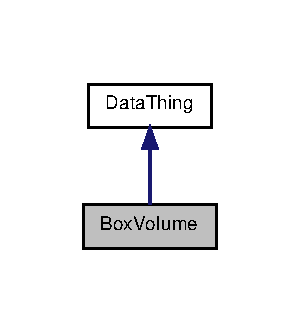
\includegraphics[width=144pt]{class_box_volume__inherit__graph}
\end{center}
\end{figure}


Collaboration diagram for BoxVolume:\nopagebreak
\begin{figure}[H]
\begin{center}
\leavevmode
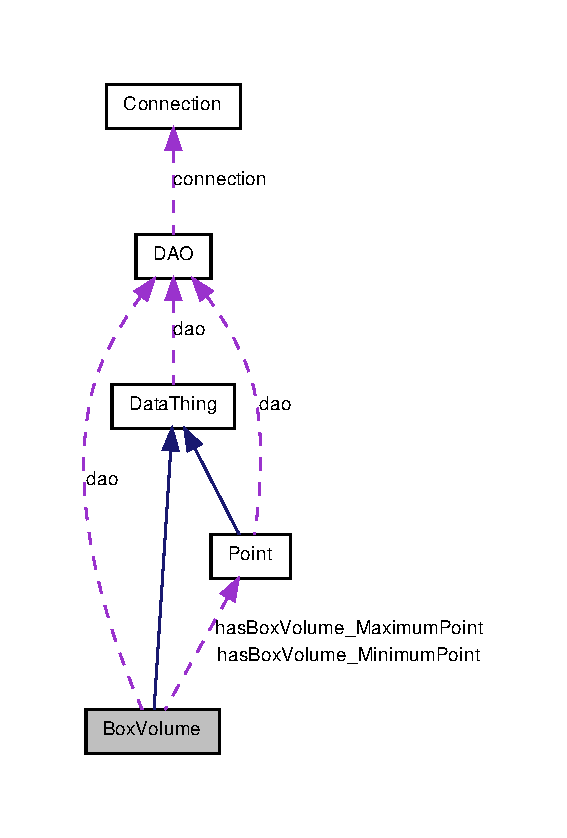
\includegraphics[width=272pt]{class_box_volume__coll__graph}
\end{center}
\end{figure}
\subsection*{Public Member Functions}
\begin{DoxyCompactItemize}
\item 
\hyperlink{class_box_volume_a495b367deb4c129983ed0771b9dd2d2b}{BoxVolume} (std::string name)
\item 
\hyperlink{class_box_volume_a5fdd6ea10bfcc6a1346840201afb3d51}{$\sim$BoxVolume} ()
\item 
void \hyperlink{class_box_volume_ad5470426b7ed060920fb0cd701a0eba7}{get} (int id)
\item 
void \hyperlink{class_box_volume_a332f433a35f192739f3570d4c8941b6a}{get} (std::string name)
\item 
void \hyperlink{class_box_volume_a5c5491a4aa1cb62946278dd3dcb91c4c}{set} (int id, \hyperlink{class_box_volume}{BoxVolume} $\ast$obj)
\item 
void \hyperlink{class_box_volume_a4aa7c183fec52b57fab6d509e5e87e5a}{set} (std::string name)
\item 
std::string \hyperlink{class_box_volume_a786f06a3a9b3c1feff8aa120b449f5de}{getname} ()
\item 
int \hyperlink{class_box_volume_a5774356e256f0574ad127371f5440fa1}{getBoxVolumeID} ()
\item 
\hyperlink{class_d_a_o}{DAO} $\ast$ \hyperlink{class_box_volume_ab39b3c8e7c434e9a963f5c538b3ee84e}{getdao} ()
\item 
void \hyperlink{class_box_volume_ad186a540505ac006ee58952ecaed35f8}{setdao} (\hyperlink{class_d_a_o}{DAO} $\ast$\_\-dao)
\item 
\hyperlink{class_point}{Point} $\ast$ \hyperlink{class_box_volume_ac71541715b68c7e97b404fadcb48e07c}{gethasBoxVolume\_\-MaximumPoint} ()
\item 
void \hyperlink{class_box_volume_ae120badf25eb21e24a200040ace7446f}{sethasBoxVolume\_\-MaximumPoint} (\hyperlink{class_point}{Point} $\ast$\_\-hasBoxVolume\_\-MaximumPoint)
\item 
\hyperlink{class_point}{Point} $\ast$ \hyperlink{class_box_volume_a735604b17ddf91a2562f40e0a03dd74f}{gethasBoxVolume\_\-MinimumPoint} ()
\item 
void \hyperlink{class_box_volume_aa08d6ff0a471dde03302c6672c5d4323}{sethasBoxVolume\_\-MinimumPoint} (\hyperlink{class_point}{Point} $\ast$\_\-hasBoxVolume\_\-MinimumPoint)
\item 
std::vector$<$ \hyperlink{class_kitting_workstation}{KittingWorkstation} $\ast$ $>$ $\ast$ \hyperlink{class_box_volume_a4676f494bb76933d5c9cd8777b2187d4}{gethasWorkstation\_\-OtherObstacles} ()
\item 
void \hyperlink{class_box_volume_a0ae9abf069ea97258cd7bf2ccdddce2b}{sethasWorkstation\_\-OtherObstacles} (std::vector$<$ \hyperlink{class_kitting_workstation}{KittingWorkstation} $\ast$ $>$ \_\-hasWorkstation\_\-OtherObstacles)
\item 
std::vector$<$ \hyperlink{class_robot}{Robot} $\ast$ $>$ $\ast$ \hyperlink{class_box_volume_a3a4e597875fa444521d459fe9bf142c3}{gethasRobot\_\-WorkVolume} ()
\item 
void \hyperlink{class_box_volume_add211d5150c8d2f8420a58030388d68f}{sethasRobot\_\-WorkVolume} (std::vector$<$ \hyperlink{class_robot}{Robot} $\ast$ $>$ \_\-hasRobot\_\-WorkVolume)
\item 
void \hyperlink{class_box_volume_a409bebf982f9e26fc5d4256b418589b2}{copy} (std::map$<$ std::string, std::string $>$ object)
\item 
std::vector$<$ std::string $>$ \hyperlink{class_box_volume_ab463d1b1327dae19a7da471a97b3f242}{Explode} (const std::string \&str, char separator)
\end{DoxyCompactItemize}


\subsection{Constructor \& Destructor Documentation}
\hypertarget{class_box_volume_a495b367deb4c129983ed0771b9dd2d2b}{
\index{BoxVolume@{BoxVolume}!BoxVolume@{BoxVolume}}
\index{BoxVolume@{BoxVolume}!BoxVolume@{BoxVolume}}
\subsubsection[{BoxVolume}]{\setlength{\rightskip}{0pt plus 5cm}BoxVolume::BoxVolume (
\begin{DoxyParamCaption}
\item[{std::string}]{name}
\end{DoxyParamCaption}
)}}
\label{class_box_volume_a495b367deb4c129983ed0771b9dd2d2b}
\hypertarget{class_box_volume_a5fdd6ea10bfcc6a1346840201afb3d51}{
\index{BoxVolume@{BoxVolume}!$\sim$BoxVolume@{$\sim$BoxVolume}}
\index{$\sim$BoxVolume@{$\sim$BoxVolume}!BoxVolume@{BoxVolume}}
\subsubsection[{$\sim$BoxVolume}]{\setlength{\rightskip}{0pt plus 5cm}BoxVolume::$\sim$BoxVolume (
\begin{DoxyParamCaption}
{}
\end{DoxyParamCaption}
)}}
\label{class_box_volume_a5fdd6ea10bfcc6a1346840201afb3d51}


\subsection{Member Function Documentation}
\hypertarget{class_box_volume_a409bebf982f9e26fc5d4256b418589b2}{
\index{BoxVolume@{BoxVolume}!copy@{copy}}
\index{copy@{copy}!BoxVolume@{BoxVolume}}
\subsubsection[{copy}]{\setlength{\rightskip}{0pt plus 5cm}void BoxVolume::copy (
\begin{DoxyParamCaption}
\item[{std::map$<$ std::string, std::string $>$}]{object}
\end{DoxyParamCaption}
)}}
\label{class_box_volume_a409bebf982f9e26fc5d4256b418589b2}


Reimplemented from \hyperlink{class_data_thing_a6d3f72340c760ce2d464fdca61a85633}{DataThing}.



Here is the call graph for this function:\nopagebreak
\begin{figure}[H]
\begin{center}
\leavevmode
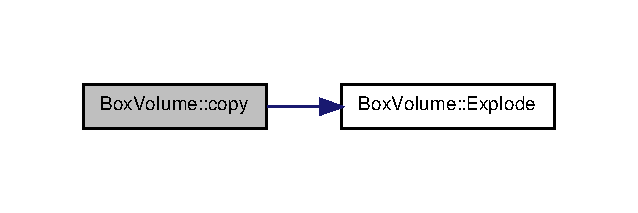
\includegraphics[width=306pt]{class_box_volume_a409bebf982f9e26fc5d4256b418589b2_cgraph}
\end{center}
\end{figure}




Here is the caller graph for this function:\nopagebreak
\begin{figure}[H]
\begin{center}
\leavevmode
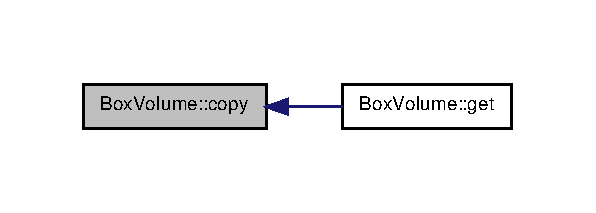
\includegraphics[width=286pt]{class_box_volume_a409bebf982f9e26fc5d4256b418589b2_icgraph}
\end{center}
\end{figure}


\hypertarget{class_box_volume_ab463d1b1327dae19a7da471a97b3f242}{
\index{BoxVolume@{BoxVolume}!Explode@{Explode}}
\index{Explode@{Explode}!BoxVolume@{BoxVolume}}
\subsubsection[{Explode}]{\setlength{\rightskip}{0pt plus 5cm}std::vector$<$ std::string $>$ BoxVolume::Explode (
\begin{DoxyParamCaption}
\item[{const std::string \&}]{str, }
\item[{char}]{separator}
\end{DoxyParamCaption}
)}}
\label{class_box_volume_ab463d1b1327dae19a7da471a97b3f242}


Reimplemented from \hyperlink{class_data_thing_ad0bf28e66a55089ee19dd2a92b71244f}{DataThing}.



Here is the caller graph for this function:\nopagebreak
\begin{figure}[H]
\begin{center}
\leavevmode
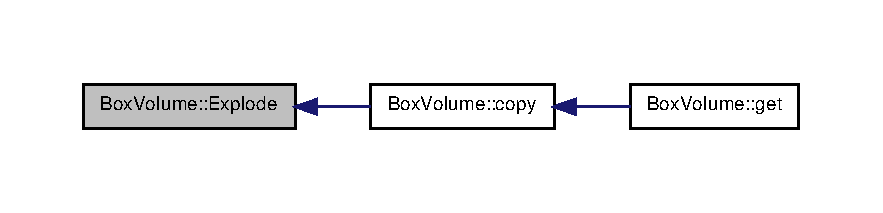
\includegraphics[width=400pt]{class_box_volume_ab463d1b1327dae19a7da471a97b3f242_icgraph}
\end{center}
\end{figure}


\hypertarget{class_box_volume_ad5470426b7ed060920fb0cd701a0eba7}{
\index{BoxVolume@{BoxVolume}!get@{get}}
\index{get@{get}!BoxVolume@{BoxVolume}}
\subsubsection[{get}]{\setlength{\rightskip}{0pt plus 5cm}void BoxVolume::get (
\begin{DoxyParamCaption}
\item[{int}]{id}
\end{DoxyParamCaption}
)}}
\label{class_box_volume_ad5470426b7ed060920fb0cd701a0eba7}


Reimplemented from \hyperlink{class_data_thing_a8d294fdb8263e02e911e429aa79e8ec0}{DataThing}.

\hypertarget{class_box_volume_a332f433a35f192739f3570d4c8941b6a}{
\index{BoxVolume@{BoxVolume}!get@{get}}
\index{get@{get}!BoxVolume@{BoxVolume}}
\subsubsection[{get}]{\setlength{\rightskip}{0pt plus 5cm}void BoxVolume::get (
\begin{DoxyParamCaption}
\item[{std::string}]{name}
\end{DoxyParamCaption}
)}}
\label{class_box_volume_a332f433a35f192739f3570d4c8941b6a}


Reimplemented from \hyperlink{class_data_thing_ac2eac975c5f135baa984906b073920e8}{DataThing}.



Here is the call graph for this function:\nopagebreak
\begin{figure}[H]
\begin{center}
\leavevmode
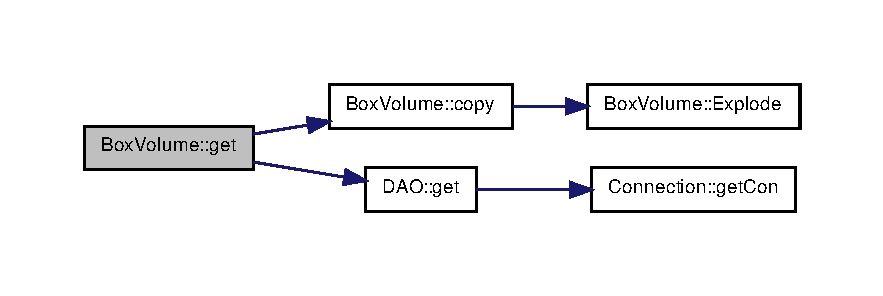
\includegraphics[width=400pt]{class_box_volume_a332f433a35f192739f3570d4c8941b6a_cgraph}
\end{center}
\end{figure}


\hypertarget{class_box_volume_a5774356e256f0574ad127371f5440fa1}{
\index{BoxVolume@{BoxVolume}!getBoxVolumeID@{getBoxVolumeID}}
\index{getBoxVolumeID@{getBoxVolumeID}!BoxVolume@{BoxVolume}}
\subsubsection[{getBoxVolumeID}]{\setlength{\rightskip}{0pt plus 5cm}int BoxVolume::getBoxVolumeID (
\begin{DoxyParamCaption}
{}
\end{DoxyParamCaption}
)}}
\label{class_box_volume_a5774356e256f0574ad127371f5440fa1}
\hypertarget{class_box_volume_ab39b3c8e7c434e9a963f5c538b3ee84e}{
\index{BoxVolume@{BoxVolume}!getdao@{getdao}}
\index{getdao@{getdao}!BoxVolume@{BoxVolume}}
\subsubsection[{getdao}]{\setlength{\rightskip}{0pt plus 5cm}{\bf DAO} $\ast$ BoxVolume::getdao (
\begin{DoxyParamCaption}
{}
\end{DoxyParamCaption}
)}}
\label{class_box_volume_ab39b3c8e7c434e9a963f5c538b3ee84e}


Reimplemented from \hyperlink{class_data_thing_ae405347375d1a67fc132f200e74637d3}{DataThing}.

\hypertarget{class_box_volume_ac71541715b68c7e97b404fadcb48e07c}{
\index{BoxVolume@{BoxVolume}!gethasBoxVolume\_\-MaximumPoint@{gethasBoxVolume\_\-MaximumPoint}}
\index{gethasBoxVolume\_\-MaximumPoint@{gethasBoxVolume\_\-MaximumPoint}!BoxVolume@{BoxVolume}}
\subsubsection[{gethasBoxVolume\_\-MaximumPoint}]{\setlength{\rightskip}{0pt plus 5cm}{\bf Point} $\ast$ BoxVolume::gethasBoxVolume\_\-MaximumPoint (
\begin{DoxyParamCaption}
{}
\end{DoxyParamCaption}
)}}
\label{class_box_volume_ac71541715b68c7e97b404fadcb48e07c}
\hypertarget{class_box_volume_a735604b17ddf91a2562f40e0a03dd74f}{
\index{BoxVolume@{BoxVolume}!gethasBoxVolume\_\-MinimumPoint@{gethasBoxVolume\_\-MinimumPoint}}
\index{gethasBoxVolume\_\-MinimumPoint@{gethasBoxVolume\_\-MinimumPoint}!BoxVolume@{BoxVolume}}
\subsubsection[{gethasBoxVolume\_\-MinimumPoint}]{\setlength{\rightskip}{0pt plus 5cm}{\bf Point} $\ast$ BoxVolume::gethasBoxVolume\_\-MinimumPoint (
\begin{DoxyParamCaption}
{}
\end{DoxyParamCaption}
)}}
\label{class_box_volume_a735604b17ddf91a2562f40e0a03dd74f}
\hypertarget{class_box_volume_a3a4e597875fa444521d459fe9bf142c3}{
\index{BoxVolume@{BoxVolume}!gethasRobot\_\-WorkVolume@{gethasRobot\_\-WorkVolume}}
\index{gethasRobot\_\-WorkVolume@{gethasRobot\_\-WorkVolume}!BoxVolume@{BoxVolume}}
\subsubsection[{gethasRobot\_\-WorkVolume}]{\setlength{\rightskip}{0pt plus 5cm}std::vector$<$ {\bf Robot} $\ast$ $>$ $\ast$ BoxVolume::gethasRobot\_\-WorkVolume (
\begin{DoxyParamCaption}
{}
\end{DoxyParamCaption}
)}}
\label{class_box_volume_a3a4e597875fa444521d459fe9bf142c3}
\hypertarget{class_box_volume_a4676f494bb76933d5c9cd8777b2187d4}{
\index{BoxVolume@{BoxVolume}!gethasWorkstation\_\-OtherObstacles@{gethasWorkstation\_\-OtherObstacles}}
\index{gethasWorkstation\_\-OtherObstacles@{gethasWorkstation\_\-OtherObstacles}!BoxVolume@{BoxVolume}}
\subsubsection[{gethasWorkstation\_\-OtherObstacles}]{\setlength{\rightskip}{0pt plus 5cm}std::vector$<$ {\bf KittingWorkstation} $\ast$ $>$ $\ast$ BoxVolume::gethasWorkstation\_\-OtherObstacles (
\begin{DoxyParamCaption}
{}
\end{DoxyParamCaption}
)}}
\label{class_box_volume_a4676f494bb76933d5c9cd8777b2187d4}
\hypertarget{class_box_volume_a786f06a3a9b3c1feff8aa120b449f5de}{
\index{BoxVolume@{BoxVolume}!getname@{getname}}
\index{getname@{getname}!BoxVolume@{BoxVolume}}
\subsubsection[{getname}]{\setlength{\rightskip}{0pt plus 5cm}std::string BoxVolume::getname (
\begin{DoxyParamCaption}
{}
\end{DoxyParamCaption}
)}}
\label{class_box_volume_a786f06a3a9b3c1feff8aa120b449f5de}


Reimplemented from \hyperlink{class_data_thing_af283145e771ef8a47c853ceed4a9f963}{DataThing}.

\hypertarget{class_box_volume_a4aa7c183fec52b57fab6d509e5e87e5a}{
\index{BoxVolume@{BoxVolume}!set@{set}}
\index{set@{set}!BoxVolume@{BoxVolume}}
\subsubsection[{set}]{\setlength{\rightskip}{0pt plus 5cm}void BoxVolume::set (
\begin{DoxyParamCaption}
\item[{std::string}]{name}
\end{DoxyParamCaption}
)}}
\label{class_box_volume_a4aa7c183fec52b57fab6d509e5e87e5a}


Reimplemented from \hyperlink{class_data_thing_a2e3a079dcb519fa810f2d6412ba90cd3}{DataThing}.



Here is the call graph for this function:\nopagebreak
\begin{figure}[H]
\begin{center}
\leavevmode
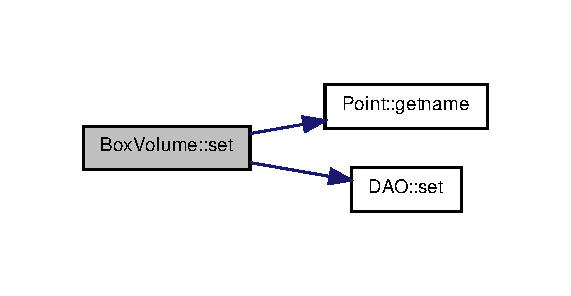
\includegraphics[width=274pt]{class_box_volume_a4aa7c183fec52b57fab6d509e5e87e5a_cgraph}
\end{center}
\end{figure}


\hypertarget{class_box_volume_a5c5491a4aa1cb62946278dd3dcb91c4c}{
\index{BoxVolume@{BoxVolume}!set@{set}}
\index{set@{set}!BoxVolume@{BoxVolume}}
\subsubsection[{set}]{\setlength{\rightskip}{0pt plus 5cm}void BoxVolume::set (
\begin{DoxyParamCaption}
\item[{int}]{id, }
\item[{{\bf BoxVolume} $\ast$}]{obj}
\end{DoxyParamCaption}
)}}
\label{class_box_volume_a5c5491a4aa1cb62946278dd3dcb91c4c}
\hypertarget{class_box_volume_ad186a540505ac006ee58952ecaed35f8}{
\index{BoxVolume@{BoxVolume}!setdao@{setdao}}
\index{setdao@{setdao}!BoxVolume@{BoxVolume}}
\subsubsection[{setdao}]{\setlength{\rightskip}{0pt plus 5cm}void BoxVolume::setdao (
\begin{DoxyParamCaption}
\item[{{\bf DAO} $\ast$}]{\_\-dao}
\end{DoxyParamCaption}
)}}
\label{class_box_volume_ad186a540505ac006ee58952ecaed35f8}


Reimplemented from \hyperlink{class_data_thing_af13c3ba6fa5e679aaa245e22b8d16e13}{DataThing}.

\hypertarget{class_box_volume_ae120badf25eb21e24a200040ace7446f}{
\index{BoxVolume@{BoxVolume}!sethasBoxVolume\_\-MaximumPoint@{sethasBoxVolume\_\-MaximumPoint}}
\index{sethasBoxVolume\_\-MaximumPoint@{sethasBoxVolume\_\-MaximumPoint}!BoxVolume@{BoxVolume}}
\subsubsection[{sethasBoxVolume\_\-MaximumPoint}]{\setlength{\rightskip}{0pt plus 5cm}void BoxVolume::sethasBoxVolume\_\-MaximumPoint (
\begin{DoxyParamCaption}
\item[{{\bf Point} $\ast$}]{\_\-hasBoxVolume\_\-MaximumPoint}
\end{DoxyParamCaption}
)}}
\label{class_box_volume_ae120badf25eb21e24a200040ace7446f}
\hypertarget{class_box_volume_aa08d6ff0a471dde03302c6672c5d4323}{
\index{BoxVolume@{BoxVolume}!sethasBoxVolume\_\-MinimumPoint@{sethasBoxVolume\_\-MinimumPoint}}
\index{sethasBoxVolume\_\-MinimumPoint@{sethasBoxVolume\_\-MinimumPoint}!BoxVolume@{BoxVolume}}
\subsubsection[{sethasBoxVolume\_\-MinimumPoint}]{\setlength{\rightskip}{0pt plus 5cm}void BoxVolume::sethasBoxVolume\_\-MinimumPoint (
\begin{DoxyParamCaption}
\item[{{\bf Point} $\ast$}]{\_\-hasBoxVolume\_\-MinimumPoint}
\end{DoxyParamCaption}
)}}
\label{class_box_volume_aa08d6ff0a471dde03302c6672c5d4323}
\hypertarget{class_box_volume_add211d5150c8d2f8420a58030388d68f}{
\index{BoxVolume@{BoxVolume}!sethasRobot\_\-WorkVolume@{sethasRobot\_\-WorkVolume}}
\index{sethasRobot\_\-WorkVolume@{sethasRobot\_\-WorkVolume}!BoxVolume@{BoxVolume}}
\subsubsection[{sethasRobot\_\-WorkVolume}]{\setlength{\rightskip}{0pt plus 5cm}void BoxVolume::sethasRobot\_\-WorkVolume (
\begin{DoxyParamCaption}
\item[{std::vector$<$ {\bf Robot} $\ast$ $>$}]{\_\-hasRobot\_\-WorkVolume}
\end{DoxyParamCaption}
)}}
\label{class_box_volume_add211d5150c8d2f8420a58030388d68f}
\hypertarget{class_box_volume_a0ae9abf069ea97258cd7bf2ccdddce2b}{
\index{BoxVolume@{BoxVolume}!sethasWorkstation\_\-OtherObstacles@{sethasWorkstation\_\-OtherObstacles}}
\index{sethasWorkstation\_\-OtherObstacles@{sethasWorkstation\_\-OtherObstacles}!BoxVolume@{BoxVolume}}
\subsubsection[{sethasWorkstation\_\-OtherObstacles}]{\setlength{\rightskip}{0pt plus 5cm}void BoxVolume::sethasWorkstation\_\-OtherObstacles (
\begin{DoxyParamCaption}
\item[{std::vector$<$ {\bf KittingWorkstation} $\ast$ $>$}]{\_\-hasWorkstation\_\-OtherObstacles}
\end{DoxyParamCaption}
)}}
\label{class_box_volume_a0ae9abf069ea97258cd7bf2ccdddce2b}


The documentation for this class was generated from the following files:\begin{DoxyCompactItemize}
\item 
/home/zeid/workspace/executor/src/database/\hyperlink{_box_volume_8h}{BoxVolume.h}\item 
/home/zeid/workspace/executor/src/database/\hyperlink{_box_volume_8cpp}{BoxVolume.cpp}\end{DoxyCompactItemize}

\hypertarget{class_boxy_object}{
\section{BoxyObject Class Reference}
\label{class_boxy_object}\index{BoxyObject@{BoxyObject}}
}


{\ttfamily \#include $<$BoxyObject.h$>$}



Inheritance diagram for BoxyObject:\nopagebreak
\begin{figure}[H]
\begin{center}
\leavevmode
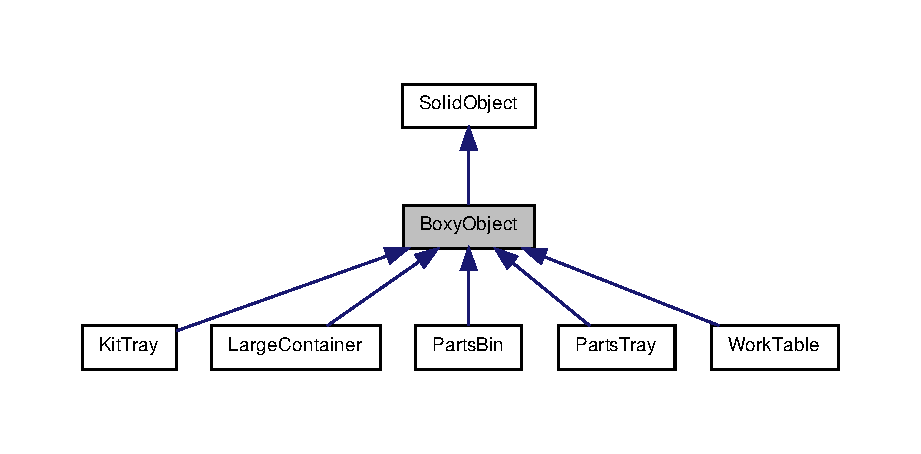
\includegraphics[width=400pt]{class_boxy_object__inherit__graph}
\end{center}
\end{figure}


Collaboration diagram for BoxyObject:\nopagebreak
\begin{figure}[H]
\begin{center}
\leavevmode
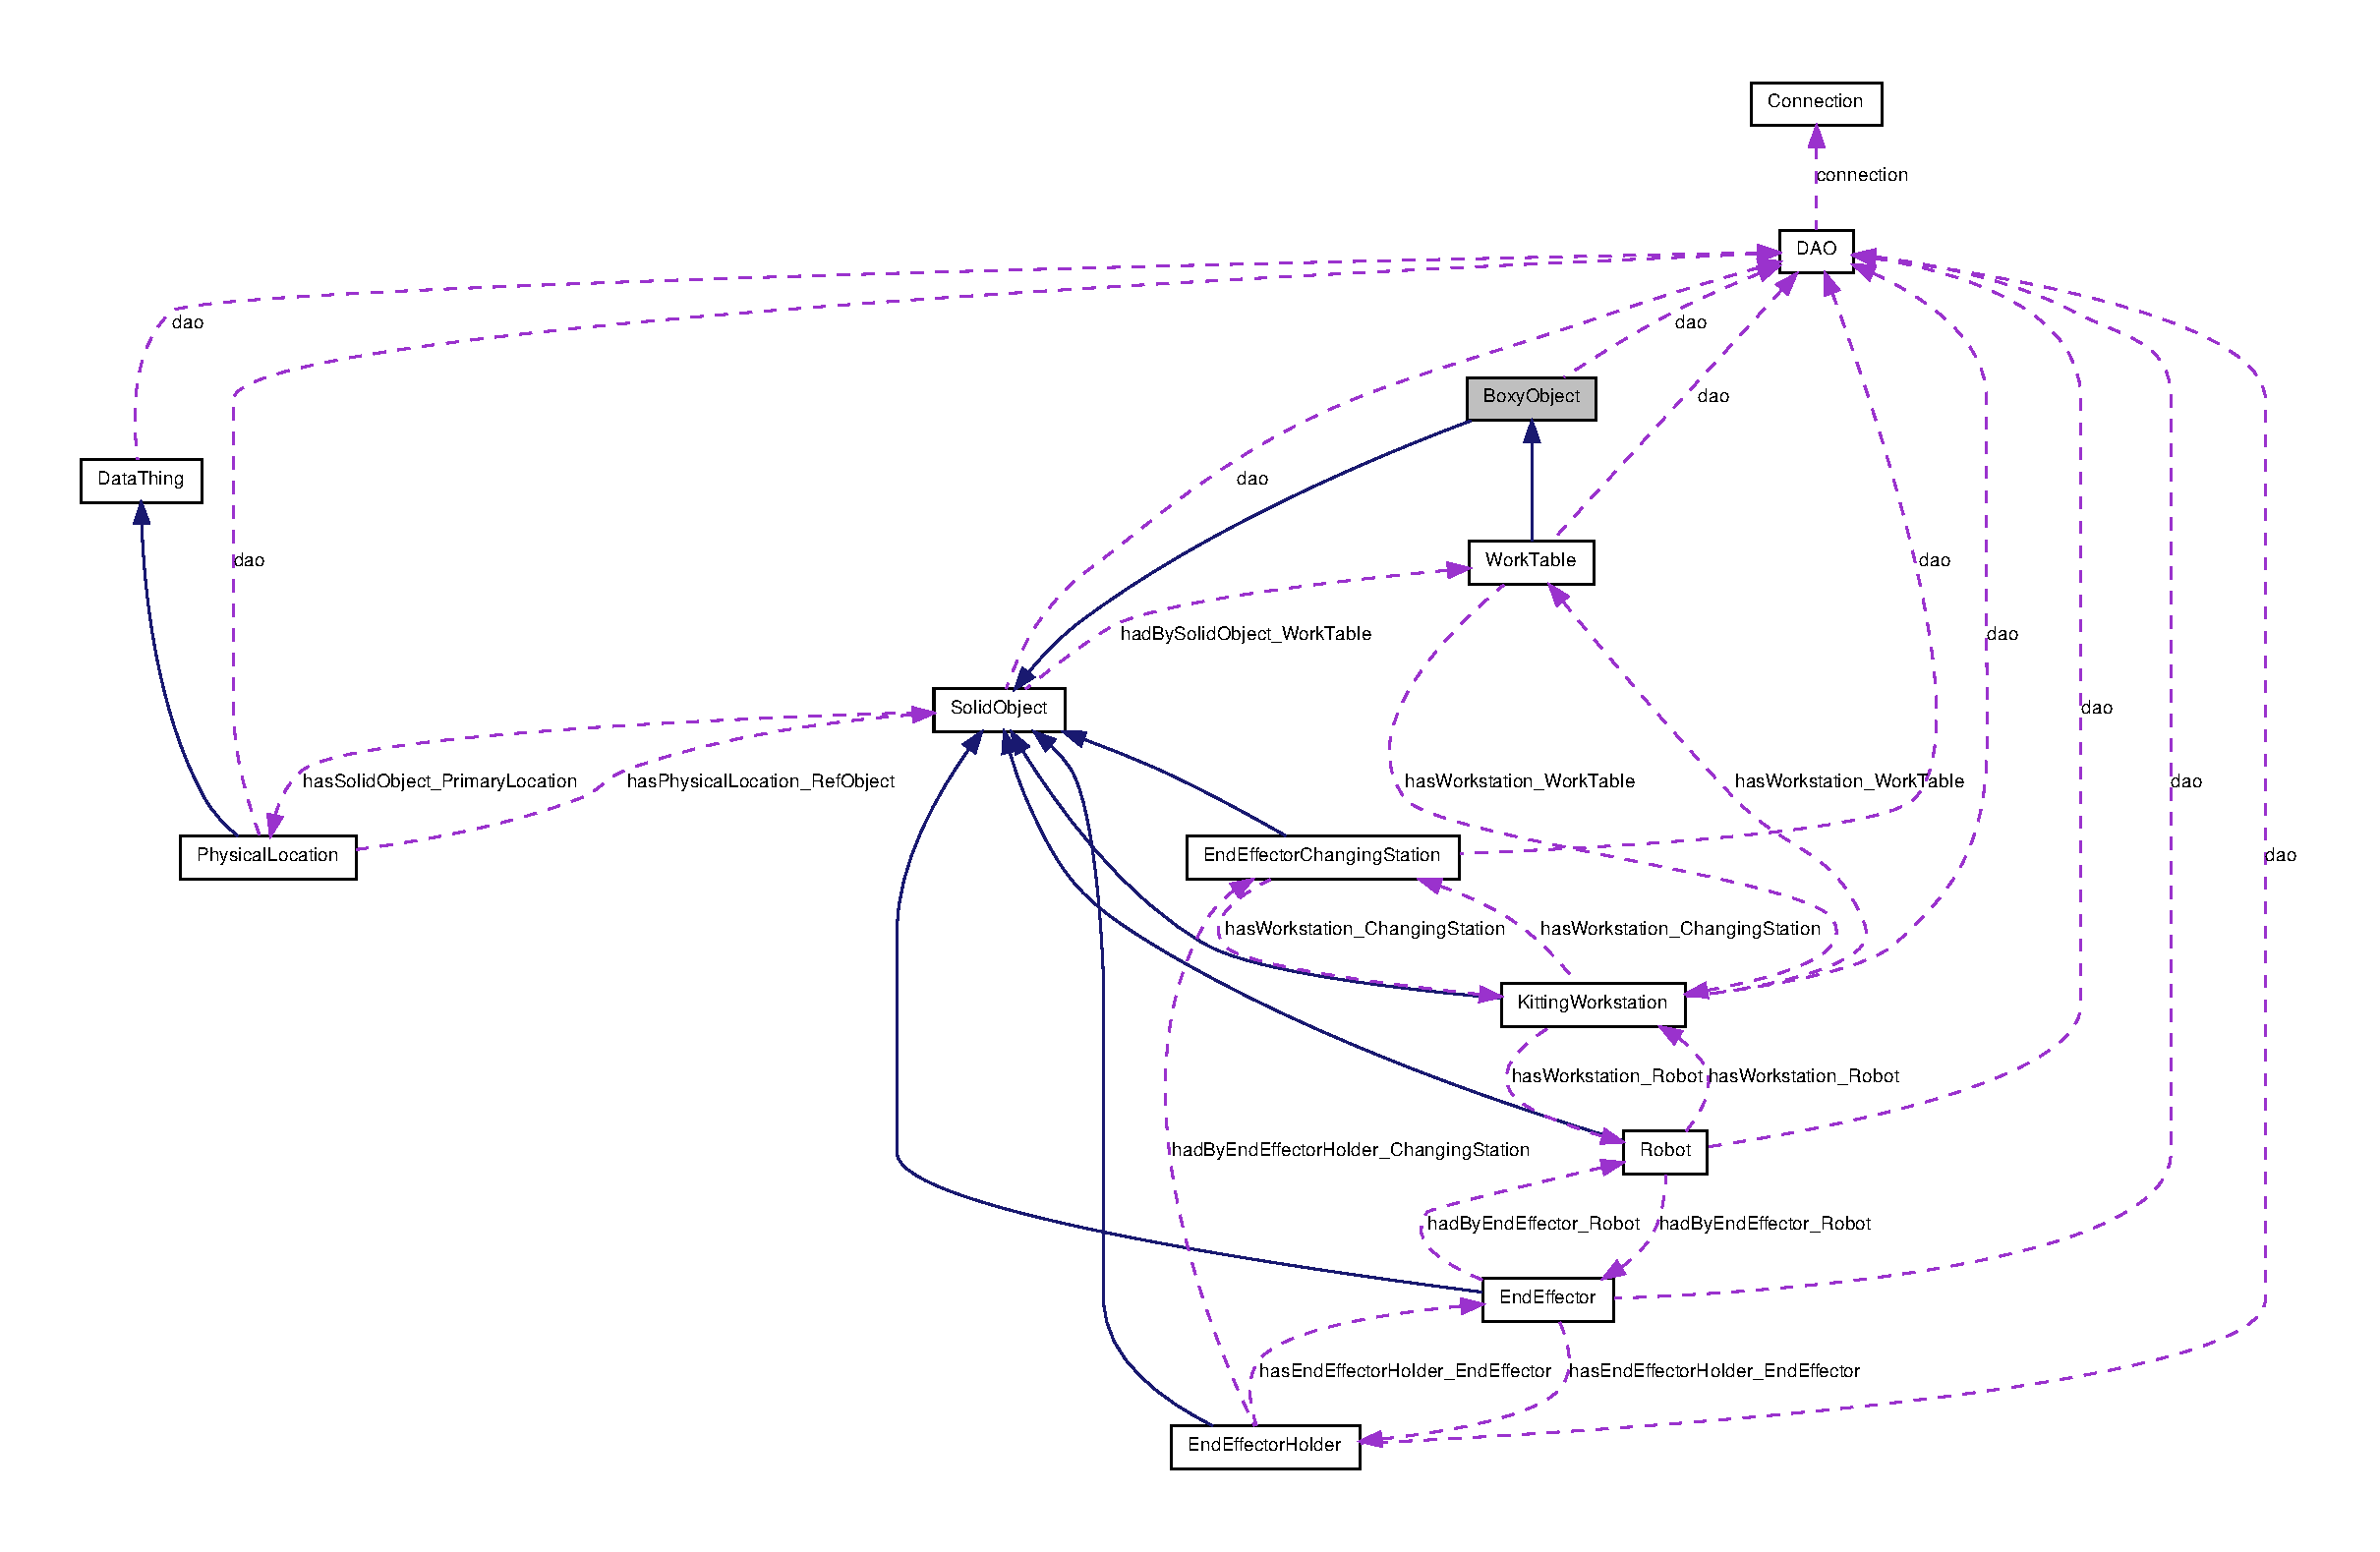
\includegraphics[width=400pt]{class_boxy_object__coll__graph}
\end{center}
\end{figure}
\subsection*{Public Member Functions}
\begin{DoxyCompactItemize}
\item 
\hyperlink{class_boxy_object_ac34b3a3838b64fdcc5d2d02c4a6bcca6}{BoxyObject} (std::string name)
\item 
\hyperlink{class_boxy_object_a93fa80f07bf6491f3a4da109fe2a2dcb}{$\sim$BoxyObject} ()
\item 
void \hyperlink{class_boxy_object_a7fdbe551740154b9be17cca9e17b5cd0}{get} (int id)
\item 
void \hyperlink{class_boxy_object_aaa4e45e5c3f830a1c0e942a8dc56e913}{get} (std::string name)
\item 
void \hyperlink{class_boxy_object_a4d1aa934a51159726e888efed2379b15}{set} (int id, \hyperlink{class_boxy_object}{BoxyObject} $\ast$obj)
\item 
void \hyperlink{class_boxy_object_a7974464a1468ea0513119cf5f843c763}{set} (std::string name)
\item 
double \hyperlink{class_boxy_object_a6aeed193c079ae3b95b3f067b7039720}{gethasBox\_\-Height} ()
\item 
void \hyperlink{class_boxy_object_a4420d3dc9e3707fe6c3079edf8b43d65}{sethasBox\_\-Height} (double \_\-hasBox\_\-Height)
\item 
double \hyperlink{class_boxy_object_a860ad5cd9341bf8d40e0a367163ef15e}{gethasBox\_\-Width} ()
\item 
void \hyperlink{class_boxy_object_aa2fe1afa5d4f23d1e0fa35e9dde920d5}{sethasBox\_\-Width} (double \_\-hasBox\_\-Width)
\item 
double \hyperlink{class_boxy_object_aad90d5fc459acfb266c1aafaa14eae92}{gethasBox\_\-Length} ()
\item 
void \hyperlink{class_boxy_object_a39abf466eb4290fc890cc6f5f4df1166}{sethasBox\_\-Length} (double \_\-hasBox\_\-Length)
\item 
std::string \hyperlink{class_boxy_object_ac088bb2ceeafc1dfa6bd008bd5a6b202}{getname} ()
\item 
int \hyperlink{class_boxy_object_ac344424a0ae9fa132924575e6b01068b}{getBoxyObjectID} ()
\item 
\hyperlink{class_d_a_o}{DAO} $\ast$ \hyperlink{class_boxy_object_ab2cd5b94e2c5256f7d2c568299bbd4e3}{getdao} ()
\item 
void \hyperlink{class_boxy_object_a1031d3686be59ed04b4d8d8bd9fd3681}{setdao} (\hyperlink{class_d_a_o}{DAO} $\ast$\_\-dao)
\item 
void \hyperlink{class_boxy_object_a3ad370f98134160310755471107c1ca0}{copy} (std::map$<$ std::string, std::string $>$ object)
\item 
std::vector$<$ std::string $>$ \hyperlink{class_boxy_object_a1d37849e12f62be2d43d72a6f9a2f3b6}{Explode} (const std::string \&str, char separator)
\end{DoxyCompactItemize}


\subsection{Constructor \& Destructor Documentation}
\hypertarget{class_boxy_object_ac34b3a3838b64fdcc5d2d02c4a6bcca6}{
\index{BoxyObject@{BoxyObject}!BoxyObject@{BoxyObject}}
\index{BoxyObject@{BoxyObject}!BoxyObject@{BoxyObject}}
\subsubsection[{BoxyObject}]{\setlength{\rightskip}{0pt plus 5cm}BoxyObject::BoxyObject (
\begin{DoxyParamCaption}
\item[{std::string}]{name}
\end{DoxyParamCaption}
)}}
\label{class_boxy_object_ac34b3a3838b64fdcc5d2d02c4a6bcca6}
\hypertarget{class_boxy_object_a93fa80f07bf6491f3a4da109fe2a2dcb}{
\index{BoxyObject@{BoxyObject}!$\sim$BoxyObject@{$\sim$BoxyObject}}
\index{$\sim$BoxyObject@{$\sim$BoxyObject}!BoxyObject@{BoxyObject}}
\subsubsection[{$\sim$BoxyObject}]{\setlength{\rightskip}{0pt plus 5cm}BoxyObject::$\sim$BoxyObject (
\begin{DoxyParamCaption}
{}
\end{DoxyParamCaption}
)}}
\label{class_boxy_object_a93fa80f07bf6491f3a4da109fe2a2dcb}


\subsection{Member Function Documentation}
\hypertarget{class_boxy_object_a3ad370f98134160310755471107c1ca0}{
\index{BoxyObject@{BoxyObject}!copy@{copy}}
\index{copy@{copy}!BoxyObject@{BoxyObject}}
\subsubsection[{copy}]{\setlength{\rightskip}{0pt plus 5cm}void BoxyObject::copy (
\begin{DoxyParamCaption}
\item[{std::map$<$ std::string, std::string $>$}]{object}
\end{DoxyParamCaption}
)}}
\label{class_boxy_object_a3ad370f98134160310755471107c1ca0}


Reimplemented from \hyperlink{class_solid_object_ac3c576278aad2366890e96889d7e24cf}{SolidObject}.



Reimplemented in \hyperlink{class_kit_tray_af1043bb5db0b1117de27c6ec4b3a113b}{KitTray}, \hyperlink{class_large_container_a49edb1d47b46abdef3ffd11704d64fd3}{LargeContainer}, \hyperlink{class_parts_bin_afb7e5abe1f22afeb3d23640d2a968c44}{PartsBin}, \hyperlink{class_parts_tray_a04a7bd17fc8b13de088bd359f3e3dbd8}{PartsTray}, and \hyperlink{class_work_table_a1096cf39ac0cfb98f27b8157f2eeacb7}{WorkTable}.



Here is the caller graph for this function:\nopagebreak
\begin{figure}[H]
\begin{center}
\leavevmode
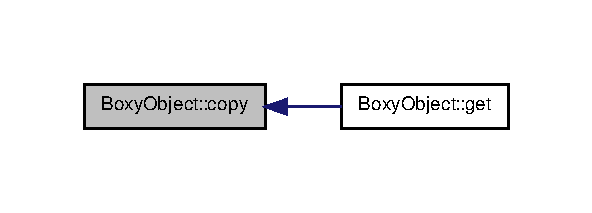
\includegraphics[width=284pt]{class_boxy_object_a3ad370f98134160310755471107c1ca0_icgraph}
\end{center}
\end{figure}


\hypertarget{class_boxy_object_a1d37849e12f62be2d43d72a6f9a2f3b6}{
\index{BoxyObject@{BoxyObject}!Explode@{Explode}}
\index{Explode@{Explode}!BoxyObject@{BoxyObject}}
\subsubsection[{Explode}]{\setlength{\rightskip}{0pt plus 5cm}std::vector$<$ std::string $>$ BoxyObject::Explode (
\begin{DoxyParamCaption}
\item[{const std::string \&}]{str, }
\item[{char}]{separator}
\end{DoxyParamCaption}
)}}
\label{class_boxy_object_a1d37849e12f62be2d43d72a6f9a2f3b6}


Reimplemented from \hyperlink{class_solid_object_a9c68e5f4e7a8bf41ab5d99736063f07c}{SolidObject}.



Reimplemented in \hyperlink{class_kit_tray_a33d1c33261e07ec6429c67e9720ed34f}{KitTray}, \hyperlink{class_large_container_a145b4b00d247f7e2d51a0ed43deec9ce}{LargeContainer}, \hyperlink{class_parts_bin_a2dd5be13c38536dc2d5f9b929fab9191}{PartsBin}, \hyperlink{class_parts_tray_a54af8fcf50c0f2ad0c45328999eaa668}{PartsTray}, and \hyperlink{class_work_table_a5bb5cd3ba5cf2095de6b4aa22db33f7e}{WorkTable}.

\hypertarget{class_boxy_object_aaa4e45e5c3f830a1c0e942a8dc56e913}{
\index{BoxyObject@{BoxyObject}!get@{get}}
\index{get@{get}!BoxyObject@{BoxyObject}}
\subsubsection[{get}]{\setlength{\rightskip}{0pt plus 5cm}void BoxyObject::get (
\begin{DoxyParamCaption}
\item[{std::string}]{name}
\end{DoxyParamCaption}
)}}
\label{class_boxy_object_aaa4e45e5c3f830a1c0e942a8dc56e913}


Reimplemented from \hyperlink{class_solid_object_afb027c9baf0d811d6f376abc10501ac9}{SolidObject}.



Reimplemented in \hyperlink{class_kit_tray_af0877c7a86b0991789a065024aa2d064}{KitTray}, \hyperlink{class_large_container_a980f922e2d6f582e29bca54bf6c66a21}{LargeContainer}, \hyperlink{class_parts_bin_acc390b70050f1074a4ff25b9f4ad9ef1}{PartsBin}, \hyperlink{class_parts_tray_a6e725e36cbe03d114ff4c1bad5acda98}{PartsTray}, and \hyperlink{class_work_table_a72e440916d93fddc774eb1e941564d0f}{WorkTable}.



Here is the call graph for this function:\nopagebreak
\begin{figure}[H]
\begin{center}
\leavevmode
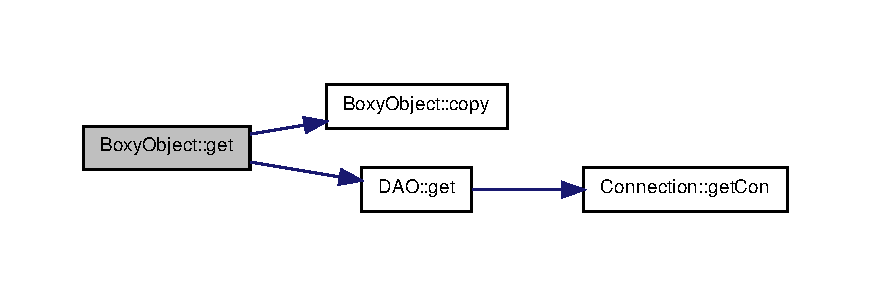
\includegraphics[width=400pt]{class_boxy_object_aaa4e45e5c3f830a1c0e942a8dc56e913_cgraph}
\end{center}
\end{figure}


\hypertarget{class_boxy_object_a7fdbe551740154b9be17cca9e17b5cd0}{
\index{BoxyObject@{BoxyObject}!get@{get}}
\index{get@{get}!BoxyObject@{BoxyObject}}
\subsubsection[{get}]{\setlength{\rightskip}{0pt plus 5cm}void BoxyObject::get (
\begin{DoxyParamCaption}
\item[{int}]{id}
\end{DoxyParamCaption}
)}}
\label{class_boxy_object_a7fdbe551740154b9be17cca9e17b5cd0}


Reimplemented from \hyperlink{class_solid_object_a76502cdc5f302d769508f196a0358d04}{SolidObject}.



Reimplemented in \hyperlink{class_kit_tray_ad153e437ec9e8e1afa9bc5ca139c5798}{KitTray}, \hyperlink{class_large_container_ab3b3f779cf410f05c813e2621ee4dc81}{LargeContainer}, \hyperlink{class_parts_bin_a7893bf99326f560b854aac9760718455}{PartsBin}, \hyperlink{class_parts_tray_a557e7cfd7075b70f8019866363984ac9}{PartsTray}, and \hyperlink{class_work_table_af112dcf025d58e18177337ae701f7af4}{WorkTable}.

\hypertarget{class_boxy_object_ac344424a0ae9fa132924575e6b01068b}{
\index{BoxyObject@{BoxyObject}!getBoxyObjectID@{getBoxyObjectID}}
\index{getBoxyObjectID@{getBoxyObjectID}!BoxyObject@{BoxyObject}}
\subsubsection[{getBoxyObjectID}]{\setlength{\rightskip}{0pt plus 5cm}int BoxyObject::getBoxyObjectID (
\begin{DoxyParamCaption}
{}
\end{DoxyParamCaption}
)}}
\label{class_boxy_object_ac344424a0ae9fa132924575e6b01068b}
\hypertarget{class_boxy_object_ab2cd5b94e2c5256f7d2c568299bbd4e3}{
\index{BoxyObject@{BoxyObject}!getdao@{getdao}}
\index{getdao@{getdao}!BoxyObject@{BoxyObject}}
\subsubsection[{getdao}]{\setlength{\rightskip}{0pt plus 5cm}{\bf DAO} $\ast$ BoxyObject::getdao (
\begin{DoxyParamCaption}
{}
\end{DoxyParamCaption}
)}}
\label{class_boxy_object_ab2cd5b94e2c5256f7d2c568299bbd4e3}


Reimplemented from \hyperlink{class_solid_object_a82697845082b48fb3b2b90606e68259a}{SolidObject}.



Reimplemented in \hyperlink{class_kit_tray_a7506daade964c5eee8a5218a7bb06bc8}{KitTray}, \hyperlink{class_large_container_abbaf38c543fed531c22dcf208e57d16d}{LargeContainer}, \hyperlink{class_parts_bin_a1dc5371ef5fb91fd1333d049568fb585}{PartsBin}, \hyperlink{class_parts_tray_a8e20e7020af9d92969bbf7709773f43f}{PartsTray}, and \hyperlink{class_work_table_a5d9f68112bb3c03985abc6fd036caac6}{WorkTable}.

\hypertarget{class_boxy_object_a6aeed193c079ae3b95b3f067b7039720}{
\index{BoxyObject@{BoxyObject}!gethasBox\_\-Height@{gethasBox\_\-Height}}
\index{gethasBox\_\-Height@{gethasBox\_\-Height}!BoxyObject@{BoxyObject}}
\subsubsection[{gethasBox\_\-Height}]{\setlength{\rightskip}{0pt plus 5cm}double BoxyObject::gethasBox\_\-Height (
\begin{DoxyParamCaption}
{}
\end{DoxyParamCaption}
)}}
\label{class_boxy_object_a6aeed193c079ae3b95b3f067b7039720}
\hypertarget{class_boxy_object_aad90d5fc459acfb266c1aafaa14eae92}{
\index{BoxyObject@{BoxyObject}!gethasBox\_\-Length@{gethasBox\_\-Length}}
\index{gethasBox\_\-Length@{gethasBox\_\-Length}!BoxyObject@{BoxyObject}}
\subsubsection[{gethasBox\_\-Length}]{\setlength{\rightskip}{0pt plus 5cm}double BoxyObject::gethasBox\_\-Length (
\begin{DoxyParamCaption}
{}
\end{DoxyParamCaption}
)}}
\label{class_boxy_object_aad90d5fc459acfb266c1aafaa14eae92}
\hypertarget{class_boxy_object_a860ad5cd9341bf8d40e0a367163ef15e}{
\index{BoxyObject@{BoxyObject}!gethasBox\_\-Width@{gethasBox\_\-Width}}
\index{gethasBox\_\-Width@{gethasBox\_\-Width}!BoxyObject@{BoxyObject}}
\subsubsection[{gethasBox\_\-Width}]{\setlength{\rightskip}{0pt plus 5cm}double BoxyObject::gethasBox\_\-Width (
\begin{DoxyParamCaption}
{}
\end{DoxyParamCaption}
)}}
\label{class_boxy_object_a860ad5cd9341bf8d40e0a367163ef15e}
\hypertarget{class_boxy_object_ac088bb2ceeafc1dfa6bd008bd5a6b202}{
\index{BoxyObject@{BoxyObject}!getname@{getname}}
\index{getname@{getname}!BoxyObject@{BoxyObject}}
\subsubsection[{getname}]{\setlength{\rightskip}{0pt plus 5cm}std::string BoxyObject::getname (
\begin{DoxyParamCaption}
{}
\end{DoxyParamCaption}
)}}
\label{class_boxy_object_ac088bb2ceeafc1dfa6bd008bd5a6b202}


Reimplemented from \hyperlink{class_solid_object_ae7b8a41f898f9463c0e298d3477fd95f}{SolidObject}.



Reimplemented in \hyperlink{class_kit_tray_a16417b0bcebb23afce3405349fe28dfd}{KitTray}, \hyperlink{class_large_container_a6274fe329979a63a5605cf39d9237ec0}{LargeContainer}, \hyperlink{class_parts_bin_a2ff289ec33d41f80ef4d11ffca65abe5}{PartsBin}, \hyperlink{class_parts_tray_a73f4b19e484bb5cbaf170b5060056037}{PartsTray}, and \hyperlink{class_work_table_ad00c3838d6e330f3f939fbbe48183eef}{WorkTable}.

\hypertarget{class_boxy_object_a4d1aa934a51159726e888efed2379b15}{
\index{BoxyObject@{BoxyObject}!set@{set}}
\index{set@{set}!BoxyObject@{BoxyObject}}
\subsubsection[{set}]{\setlength{\rightskip}{0pt plus 5cm}void BoxyObject::set (
\begin{DoxyParamCaption}
\item[{int}]{id, }
\item[{{\bf BoxyObject} $\ast$}]{obj}
\end{DoxyParamCaption}
)}}
\label{class_boxy_object_a4d1aa934a51159726e888efed2379b15}
\hypertarget{class_boxy_object_a7974464a1468ea0513119cf5f843c763}{
\index{BoxyObject@{BoxyObject}!set@{set}}
\index{set@{set}!BoxyObject@{BoxyObject}}
\subsubsection[{set}]{\setlength{\rightskip}{0pt plus 5cm}void BoxyObject::set (
\begin{DoxyParamCaption}
\item[{std::string}]{name}
\end{DoxyParamCaption}
)}}
\label{class_boxy_object_a7974464a1468ea0513119cf5f843c763}


Reimplemented from \hyperlink{class_solid_object_aaa81c29478f33c17cf15ad1409fc06b2}{SolidObject}.



Reimplemented in \hyperlink{class_kit_tray_a4b55709e9f04a99305e6a81875ee638d}{KitTray}, \hyperlink{class_large_container_af8dd74496296980354e2d45490f432ee}{LargeContainer}, \hyperlink{class_parts_bin_a31e3cbdd748787ef307978c1d1de7e06}{PartsBin}, \hyperlink{class_parts_tray_a7496bd4db3ab8833f782b48e5596b576}{PartsTray}, and \hyperlink{class_work_table_a66d9882cfeab54526a9c0d8ec9308e7c}{WorkTable}.



Here is the call graph for this function:\nopagebreak
\begin{figure}[H]
\begin{center}
\leavevmode
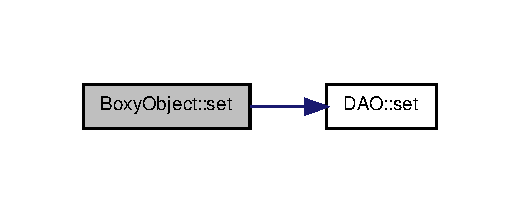
\includegraphics[width=250pt]{class_boxy_object_a7974464a1468ea0513119cf5f843c763_cgraph}
\end{center}
\end{figure}


\hypertarget{class_boxy_object_a1031d3686be59ed04b4d8d8bd9fd3681}{
\index{BoxyObject@{BoxyObject}!setdao@{setdao}}
\index{setdao@{setdao}!BoxyObject@{BoxyObject}}
\subsubsection[{setdao}]{\setlength{\rightskip}{0pt plus 5cm}void BoxyObject::setdao (
\begin{DoxyParamCaption}
\item[{{\bf DAO} $\ast$}]{\_\-dao}
\end{DoxyParamCaption}
)}}
\label{class_boxy_object_a1031d3686be59ed04b4d8d8bd9fd3681}


Reimplemented from \hyperlink{class_solid_object_aebdfc641ee348624ac5027e0a570dcd8}{SolidObject}.



Reimplemented in \hyperlink{class_kit_tray_a85651a1d085dc1702e1a29f332267c9c}{KitTray}, \hyperlink{class_large_container_a5add50911868eaa39feafcf859a81b3a}{LargeContainer}, \hyperlink{class_parts_bin_aee296552e16cfae974d5e6657454c471}{PartsBin}, \hyperlink{class_parts_tray_aed8711bfa469b61029ea4f9db477f60b}{PartsTray}, and \hyperlink{class_work_table_a715bb8e356f05a8fd25483a2dc2fc082}{WorkTable}.

\hypertarget{class_boxy_object_a4420d3dc9e3707fe6c3079edf8b43d65}{
\index{BoxyObject@{BoxyObject}!sethasBox\_\-Height@{sethasBox\_\-Height}}
\index{sethasBox\_\-Height@{sethasBox\_\-Height}!BoxyObject@{BoxyObject}}
\subsubsection[{sethasBox\_\-Height}]{\setlength{\rightskip}{0pt plus 5cm}void BoxyObject::sethasBox\_\-Height (
\begin{DoxyParamCaption}
\item[{double}]{\_\-hasBox\_\-Height}
\end{DoxyParamCaption}
)}}
\label{class_boxy_object_a4420d3dc9e3707fe6c3079edf8b43d65}
\hypertarget{class_boxy_object_a39abf466eb4290fc890cc6f5f4df1166}{
\index{BoxyObject@{BoxyObject}!sethasBox\_\-Length@{sethasBox\_\-Length}}
\index{sethasBox\_\-Length@{sethasBox\_\-Length}!BoxyObject@{BoxyObject}}
\subsubsection[{sethasBox\_\-Length}]{\setlength{\rightskip}{0pt plus 5cm}void BoxyObject::sethasBox\_\-Length (
\begin{DoxyParamCaption}
\item[{double}]{\_\-hasBox\_\-Length}
\end{DoxyParamCaption}
)}}
\label{class_boxy_object_a39abf466eb4290fc890cc6f5f4df1166}
\hypertarget{class_boxy_object_aa2fe1afa5d4f23d1e0fa35e9dde920d5}{
\index{BoxyObject@{BoxyObject}!sethasBox\_\-Width@{sethasBox\_\-Width}}
\index{sethasBox\_\-Width@{sethasBox\_\-Width}!BoxyObject@{BoxyObject}}
\subsubsection[{sethasBox\_\-Width}]{\setlength{\rightskip}{0pt plus 5cm}void BoxyObject::sethasBox\_\-Width (
\begin{DoxyParamCaption}
\item[{double}]{\_\-hasBox\_\-Width}
\end{DoxyParamCaption}
)}}
\label{class_boxy_object_aa2fe1afa5d4f23d1e0fa35e9dde920d5}


The documentation for this class was generated from the following files:\begin{DoxyCompactItemize}
\item 
/home/zeid/workspace/executor/src/database/\hyperlink{_boxy_object_8h}{BoxyObject.h}\item 
/home/zeid/workspace/executor/src/database/\hyperlink{_boxy_object_8cpp}{BoxyObject.cpp}\end{DoxyCompactItemize}

\hypertarget{struct_canonical_hdr}{
\section{CanonicalHdr Struct Reference}
\label{struct_canonical_hdr}\index{CanonicalHdr@{CanonicalHdr}}
}


{\ttfamily \#include $<$canonicalMsg.hh$>$}

\subsection*{Public Attributes}
\begin{DoxyCompactItemize}
\item 
\hyperlink{canonical_msg_8hh_a82f10f8fe974cf1c4a8c7459b963ffeb}{CanonicalType} \hyperlink{struct_canonical_hdr_a4c1a01e866dec61d147928ab40d1f292}{msgType}
\item 
unsigned int \hyperlink{struct_canonical_hdr_a0f1e839eeb5d1734e500b21db24ae808}{msgID}
\item 
double \hyperlink{struct_canonical_hdr_aa661c4ed91f577d0b0986aac7fd0c84e}{time}
\end{DoxyCompactItemize}


\subsection{Member Data Documentation}
\hypertarget{struct_canonical_hdr_a0f1e839eeb5d1734e500b21db24ae808}{
\index{CanonicalHdr@{CanonicalHdr}!msgID@{msgID}}
\index{msgID@{msgID}!CanonicalHdr@{CanonicalHdr}}
\subsubsection[{msgID}]{\setlength{\rightskip}{0pt plus 5cm}unsigned int {\bf CanonicalHdr::msgID}}}
\label{struct_canonical_hdr_a0f1e839eeb5d1734e500b21db24ae808}
\hypertarget{struct_canonical_hdr_a4c1a01e866dec61d147928ab40d1f292}{
\index{CanonicalHdr@{CanonicalHdr}!msgType@{msgType}}
\index{msgType@{msgType}!CanonicalHdr@{CanonicalHdr}}
\subsubsection[{msgType}]{\setlength{\rightskip}{0pt plus 5cm}{\bf CanonicalType} {\bf CanonicalHdr::msgType}}}
\label{struct_canonical_hdr_a4c1a01e866dec61d147928ab40d1f292}
\hypertarget{struct_canonical_hdr_aa661c4ed91f577d0b0986aac7fd0c84e}{
\index{CanonicalHdr@{CanonicalHdr}!time@{time}}
\index{time@{time}!CanonicalHdr@{CanonicalHdr}}
\subsubsection[{time}]{\setlength{\rightskip}{0pt plus 5cm}double {\bf CanonicalHdr::time}}}
\label{struct_canonical_hdr_aa661c4ed91f577d0b0986aac7fd0c84e}


The documentation for this struct was generated from the following file:\begin{DoxyCompactItemize}
\item 
/home/zeid/workspace/executor/src/controller/\hyperlink{canonical_msg_8hh}{canonicalMsg.hh}\end{DoxyCompactItemize}

\hypertarget{class_canonical_msg}{
\section{CanonicalMsg Class Reference}
\label{class_canonical_msg}\index{CanonicalMsg@{CanonicalMsg}}
}


{\ttfamily \#include $<$canonicalMsg.hh$>$}



Inheritance diagram for CanonicalMsg:\nopagebreak
\begin{figure}[H]
\begin{center}
\leavevmode
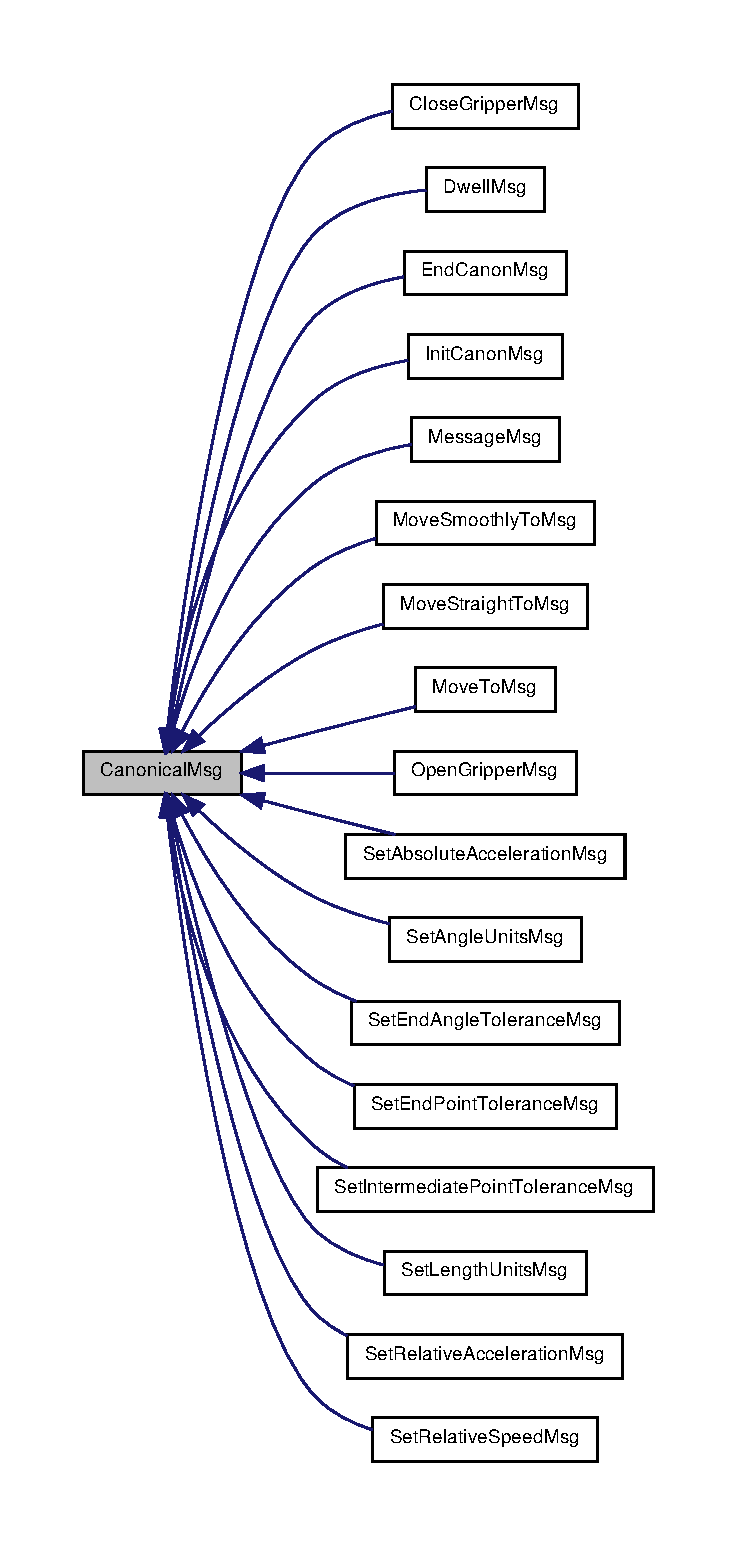
\includegraphics[height=600pt]{class_canonical_msg__inherit__graph}
\end{center}
\end{figure}


Collaboration diagram for CanonicalMsg:\nopagebreak
\begin{figure}[H]
\begin{center}
\leavevmode
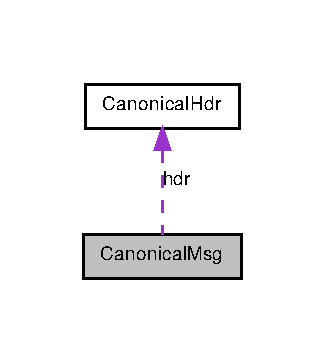
\includegraphics[width=156pt]{class_canonical_msg__coll__graph}
\end{center}
\end{figure}
\subsection*{Public Member Functions}
\begin{DoxyCompactItemize}
\item 
\hyperlink{class_canonical_msg_af352cb8576a7da3b756bf736c5e783da}{CanonicalMsg} (\hyperlink{canonical_msg_8hh_a82f10f8fe974cf1c4a8c7459b963ffeb}{CanonicalType} msgType)
\item 
void \hyperlink{class_canonical_msg_abfade49de8c1337f3f3690aa209f705b}{setHeader} ()
\item 
int \hyperlink{class_canonical_msg_a56011cb08f9e95be9423be7284876f74}{getMsgID} ()
\item 
double \hyperlink{class_canonical_msg_ace23472b599f3cd890b6080b5e0363e5}{getTime} ()
\item 
\hyperlink{canonical_msg_8hh_a82f10f8fe974cf1c4a8c7459b963ffeb}{CanonicalType} \hyperlink{class_canonical_msg_a4b13a61095d109722c40aaf0a66b30c2}{getType} ()
\end{DoxyCompactItemize}
\subsection*{Protected Attributes}
\begin{DoxyCompactItemize}
\item 
\hyperlink{struct_canonical_hdr}{CanonicalHdr} \hyperlink{class_canonical_msg_afce1fd35cf068067b013162e2b624b64}{hdr}
\end{DoxyCompactItemize}
\subsection*{Static Protected Attributes}
\begin{DoxyCompactItemize}
\item 
static int \hyperlink{class_canonical_msg_a2fc5e5c814ce88032683695e88b5f8f1}{nextID} = 1
\end{DoxyCompactItemize}


\subsection{Constructor \& Destructor Documentation}
\hypertarget{class_canonical_msg_af352cb8576a7da3b756bf736c5e783da}{
\index{CanonicalMsg@{CanonicalMsg}!CanonicalMsg@{CanonicalMsg}}
\index{CanonicalMsg@{CanonicalMsg}!CanonicalMsg@{CanonicalMsg}}
\subsubsection[{CanonicalMsg}]{\setlength{\rightskip}{0pt plus 5cm}CanonicalMsg::CanonicalMsg (
\begin{DoxyParamCaption}
\item[{{\bf CanonicalType}}]{msgType}
\end{DoxyParamCaption}
)\hspace{0.3cm}{\ttfamily  \mbox{[}inline\mbox{]}}}}
\label{class_canonical_msg_af352cb8576a7da3b756bf736c5e783da}


\subsection{Member Function Documentation}
\hypertarget{class_canonical_msg_a56011cb08f9e95be9423be7284876f74}{
\index{CanonicalMsg@{CanonicalMsg}!getMsgID@{getMsgID}}
\index{getMsgID@{getMsgID}!CanonicalMsg@{CanonicalMsg}}
\subsubsection[{getMsgID}]{\setlength{\rightskip}{0pt plus 5cm}int CanonicalMsg::getMsgID (
\begin{DoxyParamCaption}
{}
\end{DoxyParamCaption}
)\hspace{0.3cm}{\ttfamily  \mbox{[}inline\mbox{]}}}}
\label{class_canonical_msg_a56011cb08f9e95be9423be7284876f74}


Here is the caller graph for this function:\nopagebreak
\begin{figure}[H]
\begin{center}
\leavevmode
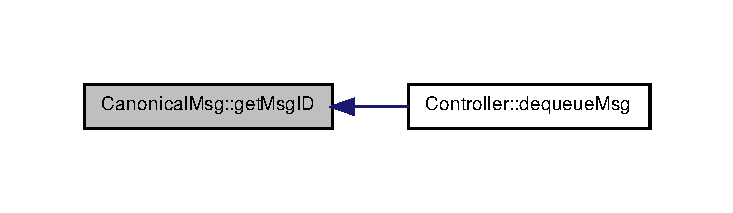
\includegraphics[width=352pt]{class_canonical_msg_a56011cb08f9e95be9423be7284876f74_icgraph}
\end{center}
\end{figure}


\hypertarget{class_canonical_msg_ace23472b599f3cd890b6080b5e0363e5}{
\index{CanonicalMsg@{CanonicalMsg}!getTime@{getTime}}
\index{getTime@{getTime}!CanonicalMsg@{CanonicalMsg}}
\subsubsection[{getTime}]{\setlength{\rightskip}{0pt plus 5cm}double CanonicalMsg::getTime (
\begin{DoxyParamCaption}
{}
\end{DoxyParamCaption}
)\hspace{0.3cm}{\ttfamily  \mbox{[}inline\mbox{]}}}}
\label{class_canonical_msg_ace23472b599f3cd890b6080b5e0363e5}


Here is the caller graph for this function:\nopagebreak
\begin{figure}[H]
\begin{center}
\leavevmode
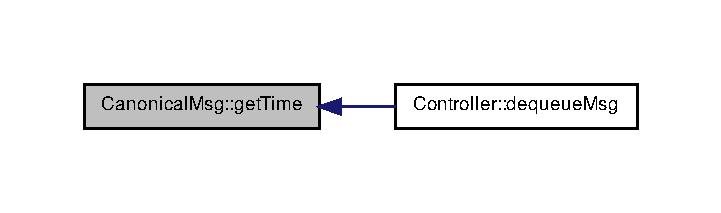
\includegraphics[width=346pt]{class_canonical_msg_ace23472b599f3cd890b6080b5e0363e5_icgraph}
\end{center}
\end{figure}


\hypertarget{class_canonical_msg_a4b13a61095d109722c40aaf0a66b30c2}{
\index{CanonicalMsg@{CanonicalMsg}!getType@{getType}}
\index{getType@{getType}!CanonicalMsg@{CanonicalMsg}}
\subsubsection[{getType}]{\setlength{\rightskip}{0pt plus 5cm}{\bf CanonicalType} CanonicalMsg::getType (
\begin{DoxyParamCaption}
{}
\end{DoxyParamCaption}
)\hspace{0.3cm}{\ttfamily  \mbox{[}inline\mbox{]}}}}
\label{class_canonical_msg_a4b13a61095d109722c40aaf0a66b30c2}


Here is the caller graph for this function:\nopagebreak
\begin{figure}[H]
\begin{center}
\leavevmode
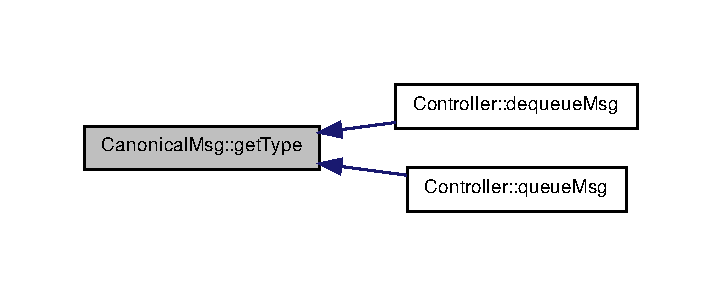
\includegraphics[width=346pt]{class_canonical_msg_a4b13a61095d109722c40aaf0a66b30c2_icgraph}
\end{center}
\end{figure}


\hypertarget{class_canonical_msg_abfade49de8c1337f3f3690aa209f705b}{
\index{CanonicalMsg@{CanonicalMsg}!setHeader@{setHeader}}
\index{setHeader@{setHeader}!CanonicalMsg@{CanonicalMsg}}
\subsubsection[{setHeader}]{\setlength{\rightskip}{0pt plus 5cm}void CanonicalMsg::setHeader (
\begin{DoxyParamCaption}
{}
\end{DoxyParamCaption}
)\hspace{0.3cm}{\ttfamily  \mbox{[}inline\mbox{]}}}}
\label{class_canonical_msg_abfade49de8c1337f3f3690aa209f705b}


Here is the call graph for this function:\nopagebreak
\begin{figure}[H]
\begin{center}
\leavevmode
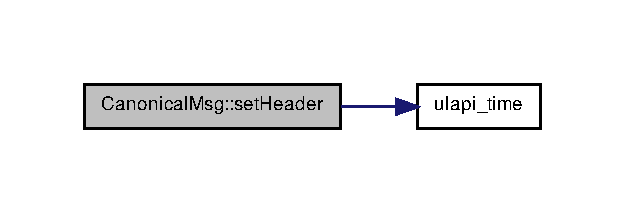
\includegraphics[width=300pt]{class_canonical_msg_abfade49de8c1337f3f3690aa209f705b_cgraph}
\end{center}
\end{figure}




Here is the caller graph for this function:\nopagebreak
\begin{figure}[H]
\begin{center}
\leavevmode
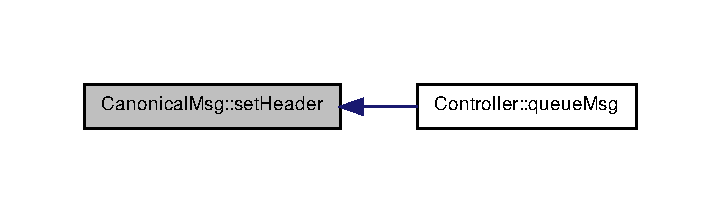
\includegraphics[width=346pt]{class_canonical_msg_abfade49de8c1337f3f3690aa209f705b_icgraph}
\end{center}
\end{figure}




\subsection{Member Data Documentation}
\hypertarget{class_canonical_msg_afce1fd35cf068067b013162e2b624b64}{
\index{CanonicalMsg@{CanonicalMsg}!hdr@{hdr}}
\index{hdr@{hdr}!CanonicalMsg@{CanonicalMsg}}
\subsubsection[{hdr}]{\setlength{\rightskip}{0pt plus 5cm}{\bf CanonicalHdr} {\bf CanonicalMsg::hdr}\hspace{0.3cm}{\ttfamily  \mbox{[}protected\mbox{]}}}}
\label{class_canonical_msg_afce1fd35cf068067b013162e2b624b64}
\hypertarget{class_canonical_msg_a2fc5e5c814ce88032683695e88b5f8f1}{
\index{CanonicalMsg@{CanonicalMsg}!nextID@{nextID}}
\index{nextID@{nextID}!CanonicalMsg@{CanonicalMsg}}
\subsubsection[{nextID}]{\setlength{\rightskip}{0pt plus 5cm}int {\bf CanonicalMsg::nextID} = 1\hspace{0.3cm}{\ttfamily  \mbox{[}static, protected\mbox{]}}}}
\label{class_canonical_msg_a2fc5e5c814ce88032683695e88b5f8f1}


The documentation for this class was generated from the following files:\begin{DoxyCompactItemize}
\item 
/home/zeid/workspace/executor/src/controller/\hyperlink{canonical_msg_8hh}{canonicalMsg.hh}\item 
/home/zeid/workspace/executor/src/controller/\hyperlink{controller_8cpp}{controller.cpp}\end{DoxyCompactItemize}

\hypertarget{class_canonical_robot_command}{
\section{CanonicalRobotCommand Class Reference}
\label{class_canonical_robot_command}\index{CanonicalRobotCommand@{CanonicalRobotCommand}}
}


{\ttfamily \#include $<$CanonicalRobotCommand.h$>$}

\subsection*{Public Member Functions}
\begin{DoxyCompactItemize}
\item 
\hyperlink{class_canonical_robot_command_a26b956d2026a0733c136bfdf57d74477}{CanonicalRobotCommand} ()
\begin{DoxyCompactList}\small\item\em Auto-\/generated constructor stub. \item\end{DoxyCompactList}\item 
virtual \hyperlink{class_canonical_robot_command_a7ab8d0a17a3554878ff5aba8c9170936}{$\sim$CanonicalRobotCommand} ()
\begin{DoxyCompactList}\small\item\em Auto-\/generated destructor stub. \item\end{DoxyCompactList}\item 
void \hyperlink{class_canonical_robot_command_a10f1fb20f4c17d0a37b747356378f29c}{actionInterpreter} (string action, vector$<$ string $>$ paramName, \hyperlink{class_kitting_plan}{KittingPlan} $\ast$kittingplan)
\begin{DoxyCompactList}\small\item\em Reads a line of the plan and interprets it into one or more canonical robot commands. \item\end{DoxyCompactList}\item 
void \hyperlink{class_canonical_robot_command_a8b54b12dc029042eedfa15598f671ac6}{interpretPlan} (\hyperlink{class_kitting_plan}{KittingPlan} $\ast$kittingplan)
\begin{DoxyCompactList}\small\item\em Read the plan stored in \hyperlink{class_kitting_plan_a8293312cf9137906c868994b4ade4587}{KittingPlan::m\_\-actionParamList} and interpret each action. \item\end{DoxyCompactList}\item 
string \hyperlink{class_canonical_robot_command_a618b3d744e3397aa81d2b95e276fefcd}{getActionName} (string myList)
\item 
void \hyperlink{class_canonical_robot_command_abc17012640ae9203f090bcdb828c9c0d}{take\_\-kit\_\-tray} (vector$<$ string $>$ paramList)
\item 
void \hyperlink{class_canonical_robot_command_a5b86751ba4697428c741709d0ac80528}{put\_\-kit\_\-tray} (vector$<$ string $>$ paramList)
\item 
void \hyperlink{class_canonical_robot_command_a33abd5938bb8c1d94bc3616609e418c5}{take\_\-kit} (vector$<$ string $>$ paramList)
\item 
void \hyperlink{class_canonical_robot_command_afa48a098e02e9fa34706b251601ca287}{put\_\-kit} (vector$<$ string $>$ paramList)
\item 
void \hyperlink{class_canonical_robot_command_afb89d61a62c1dea47f5abef6b5ec1b4e}{take\_\-part} (vector$<$ string $>$ paramList)
\item 
void \hyperlink{class_canonical_robot_command_af366c12a510324c0cd9a5d1ee17476a7}{put\_\-part} (vector$<$ string $>$ paramList)
\item 
void \hyperlink{class_canonical_robot_command_a02916ca791c56cae1a4b71c35db8753e}{attach\_\-eff} (vector$<$ string $>$ paramList, \hyperlink{class_kitting_plan}{KittingPlan} $\ast$kittingplan)
\item 
void \hyperlink{class_canonical_robot_command_a6e00f038ab69fb6a6d2f9b3c5882e789}{remove\_\-eff} (vector$<$ string $>$ paramList)
\item 
void \hyperlink{class_canonical_robot_command_a98cf18620e86ce0fce18bc7d30b9a188}{create\_\-kit} (vector$<$ string $>$ paramList)
\end{DoxyCompactItemize}


\subsection{Constructor \& Destructor Documentation}
\hypertarget{class_canonical_robot_command_a26b956d2026a0733c136bfdf57d74477}{
\index{CanonicalRobotCommand@{CanonicalRobotCommand}!CanonicalRobotCommand@{CanonicalRobotCommand}}
\index{CanonicalRobotCommand@{CanonicalRobotCommand}!CanonicalRobotCommand@{CanonicalRobotCommand}}
\subsubsection[{CanonicalRobotCommand}]{\setlength{\rightskip}{0pt plus 5cm}CanonicalRobotCommand::CanonicalRobotCommand (
\begin{DoxyParamCaption}
{}
\end{DoxyParamCaption}
)}}
\label{class_canonical_robot_command_a26b956d2026a0733c136bfdf57d74477}


Auto-\/generated constructor stub. 

\hypertarget{class_canonical_robot_command_a7ab8d0a17a3554878ff5aba8c9170936}{
\index{CanonicalRobotCommand@{CanonicalRobotCommand}!$\sim$CanonicalRobotCommand@{$\sim$CanonicalRobotCommand}}
\index{$\sim$CanonicalRobotCommand@{$\sim$CanonicalRobotCommand}!CanonicalRobotCommand@{CanonicalRobotCommand}}
\subsubsection[{$\sim$CanonicalRobotCommand}]{\setlength{\rightskip}{0pt plus 5cm}CanonicalRobotCommand::$\sim$CanonicalRobotCommand (
\begin{DoxyParamCaption}
{}
\end{DoxyParamCaption}
)\hspace{0.3cm}{\ttfamily  \mbox{[}virtual\mbox{]}}}}
\label{class_canonical_robot_command_a7ab8d0a17a3554878ff5aba8c9170936}


Auto-\/generated destructor stub. 



\subsection{Member Function Documentation}
\hypertarget{class_canonical_robot_command_a10f1fb20f4c17d0a37b747356378f29c}{
\index{CanonicalRobotCommand@{CanonicalRobotCommand}!actionInterpreter@{actionInterpreter}}
\index{actionInterpreter@{actionInterpreter}!CanonicalRobotCommand@{CanonicalRobotCommand}}
\subsubsection[{actionInterpreter}]{\setlength{\rightskip}{0pt plus 5cm}void CanonicalRobotCommand::actionInterpreter (
\begin{DoxyParamCaption}
\item[{string}]{actionName, }
\item[{vector$<$ string $>$}]{paramList, }
\item[{{\bf KittingPlan} $\ast$}]{kittingplan}
\end{DoxyParamCaption}
)}}
\label{class_canonical_robot_command_a10f1fb20f4c17d0a37b747356378f29c}


Reads a line of the plan and interprets it into one or more canonical robot commands. 


\begin{DoxyParams}{Parameters}
{\em action} & Action to be interpreted \\
\hline
\end{DoxyParams}
\begin{DoxyReturn}{Returns}
A list of commands associated to the action {\itshape action\/} 
\end{DoxyReturn}


Here is the call graph for this function:
\nopagebreak
\begin{figure}[H]
\begin{center}
\leavevmode
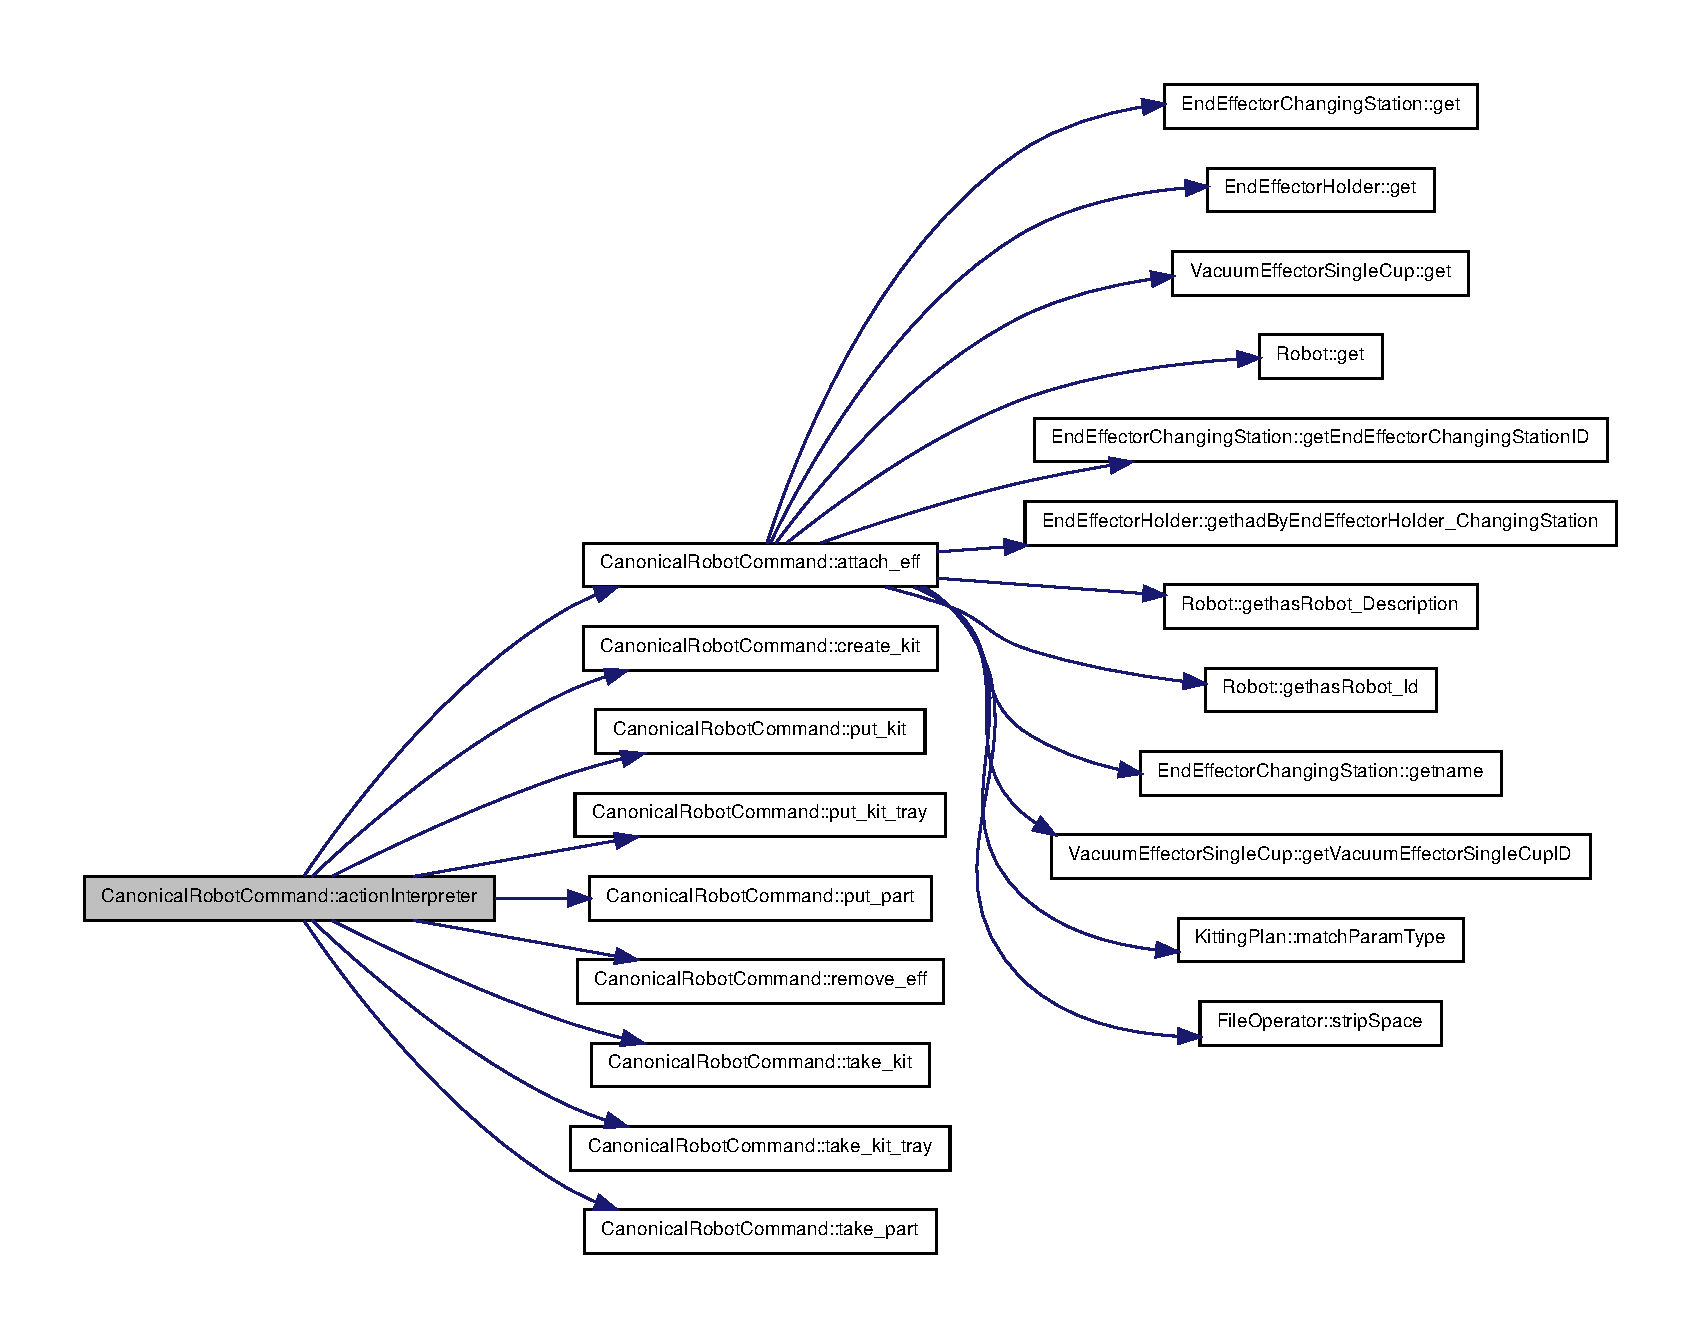
\includegraphics[width=400pt]{class_canonical_robot_command_a10f1fb20f4c17d0a37b747356378f29c_cgraph}
\end{center}
\end{figure}




Here is the caller graph for this function:
\nopagebreak
\begin{figure}[H]
\begin{center}
\leavevmode
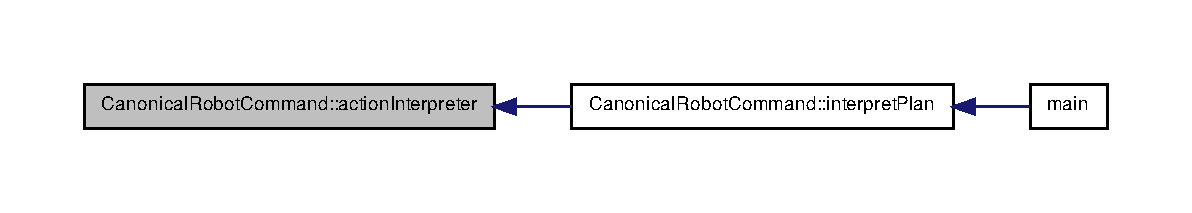
\includegraphics[width=400pt]{class_canonical_robot_command_a10f1fb20f4c17d0a37b747356378f29c_icgraph}
\end{center}
\end{figure}


\hypertarget{class_canonical_robot_command_a02916ca791c56cae1a4b71c35db8753e}{
\index{CanonicalRobotCommand@{CanonicalRobotCommand}!attach\_\-eff@{attach\_\-eff}}
\index{attach\_\-eff@{attach\_\-eff}!CanonicalRobotCommand@{CanonicalRobotCommand}}
\subsubsection[{attach\_\-eff}]{\setlength{\rightskip}{0pt plus 5cm}void CanonicalRobotCommand::attach\_\-eff (
\begin{DoxyParamCaption}
\item[{vector$<$ string $>$}]{paramList, }
\item[{{\bf KittingPlan} $\ast$}]{kittingplan}
\end{DoxyParamCaption}
)}}
\label{class_canonical_robot_command_a02916ca791c56cae1a4b71c35db8753e}


Here is the call graph for this function:
\nopagebreak
\begin{figure}[H]
\begin{center}
\leavevmode
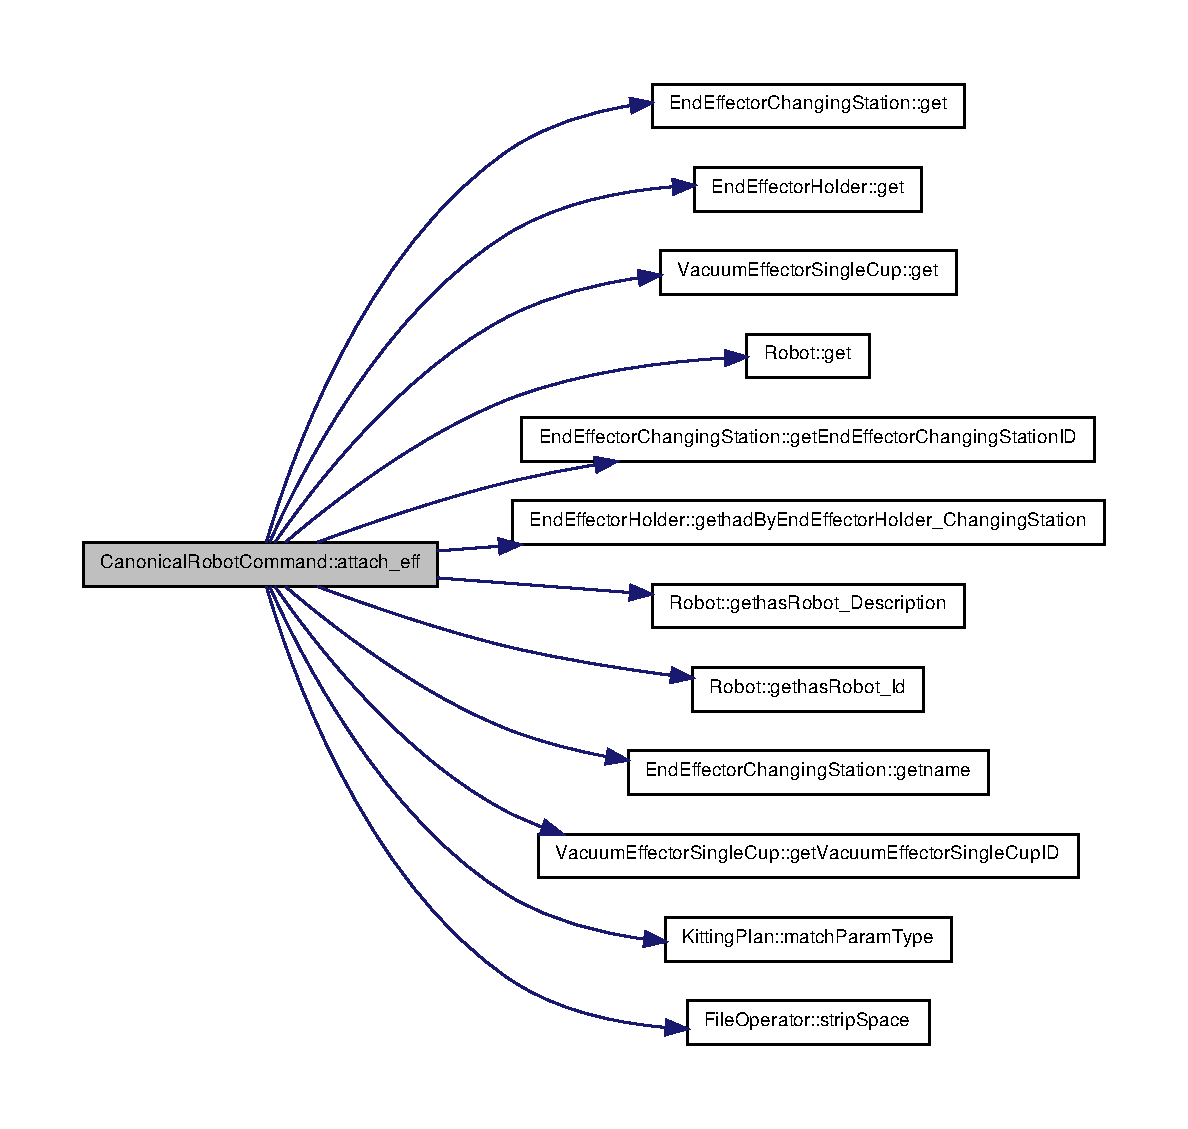
\includegraphics[width=400pt]{class_canonical_robot_command_a02916ca791c56cae1a4b71c35db8753e_cgraph}
\end{center}
\end{figure}




Here is the caller graph for this function:
\nopagebreak
\begin{figure}[H]
\begin{center}
\leavevmode
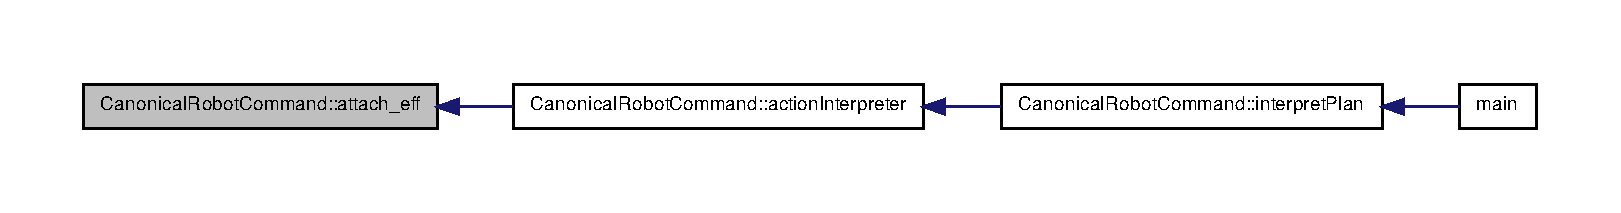
\includegraphics[width=400pt]{class_canonical_robot_command_a02916ca791c56cae1a4b71c35db8753e_icgraph}
\end{center}
\end{figure}


\hypertarget{class_canonical_robot_command_a98cf18620e86ce0fce18bc7d30b9a188}{
\index{CanonicalRobotCommand@{CanonicalRobotCommand}!create\_\-kit@{create\_\-kit}}
\index{create\_\-kit@{create\_\-kit}!CanonicalRobotCommand@{CanonicalRobotCommand}}
\subsubsection[{create\_\-kit}]{\setlength{\rightskip}{0pt plus 5cm}void CanonicalRobotCommand::create\_\-kit (
\begin{DoxyParamCaption}
\item[{vector$<$ string $>$}]{paramList}
\end{DoxyParamCaption}
)}}
\label{class_canonical_robot_command_a98cf18620e86ce0fce18bc7d30b9a188}


Here is the caller graph for this function:
\nopagebreak
\begin{figure}[H]
\begin{center}
\leavevmode
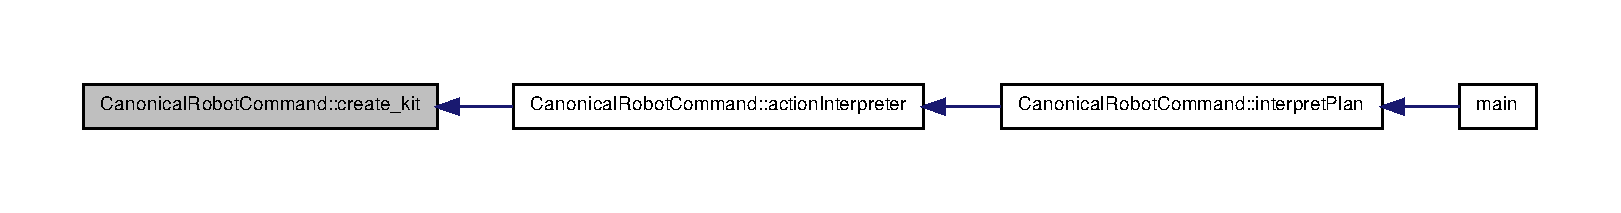
\includegraphics[width=400pt]{class_canonical_robot_command_a98cf18620e86ce0fce18bc7d30b9a188_icgraph}
\end{center}
\end{figure}


\hypertarget{class_canonical_robot_command_a618b3d744e3397aa81d2b95e276fefcd}{
\index{CanonicalRobotCommand@{CanonicalRobotCommand}!getActionName@{getActionName}}
\index{getActionName@{getActionName}!CanonicalRobotCommand@{CanonicalRobotCommand}}
\subsubsection[{getActionName}]{\setlength{\rightskip}{0pt plus 5cm}string CanonicalRobotCommand::getActionName (
\begin{DoxyParamCaption}
\item[{string}]{myList}
\end{DoxyParamCaption}
)}}
\label{class_canonical_robot_command_a618b3d744e3397aa81d2b95e276fefcd}
\hypertarget{class_canonical_robot_command_a8b54b12dc029042eedfa15598f671ac6}{
\index{CanonicalRobotCommand@{CanonicalRobotCommand}!interpretPlan@{interpretPlan}}
\index{interpretPlan@{interpretPlan}!CanonicalRobotCommand@{CanonicalRobotCommand}}
\subsubsection[{interpretPlan}]{\setlength{\rightskip}{0pt plus 5cm}void CanonicalRobotCommand::interpretPlan (
\begin{DoxyParamCaption}
\item[{{\bf KittingPlan} $\ast$}]{kittingplan}
\end{DoxyParamCaption}
)}}
\label{class_canonical_robot_command_a8b54b12dc029042eedfa15598f671ac6}


Read the plan stored in \hyperlink{class_kitting_plan_a8293312cf9137906c868994b4ade4587}{KittingPlan::m\_\-actionParamList} and interpret each action. 


\begin{DoxyParams}{Parameters}
{\em kittingplan} & Instance of \hyperlink{class_kitting_plan}{KittingPlan} \\
\hline
\end{DoxyParams}


Here is the call graph for this function:
\nopagebreak
\begin{figure}[H]
\begin{center}
\leavevmode
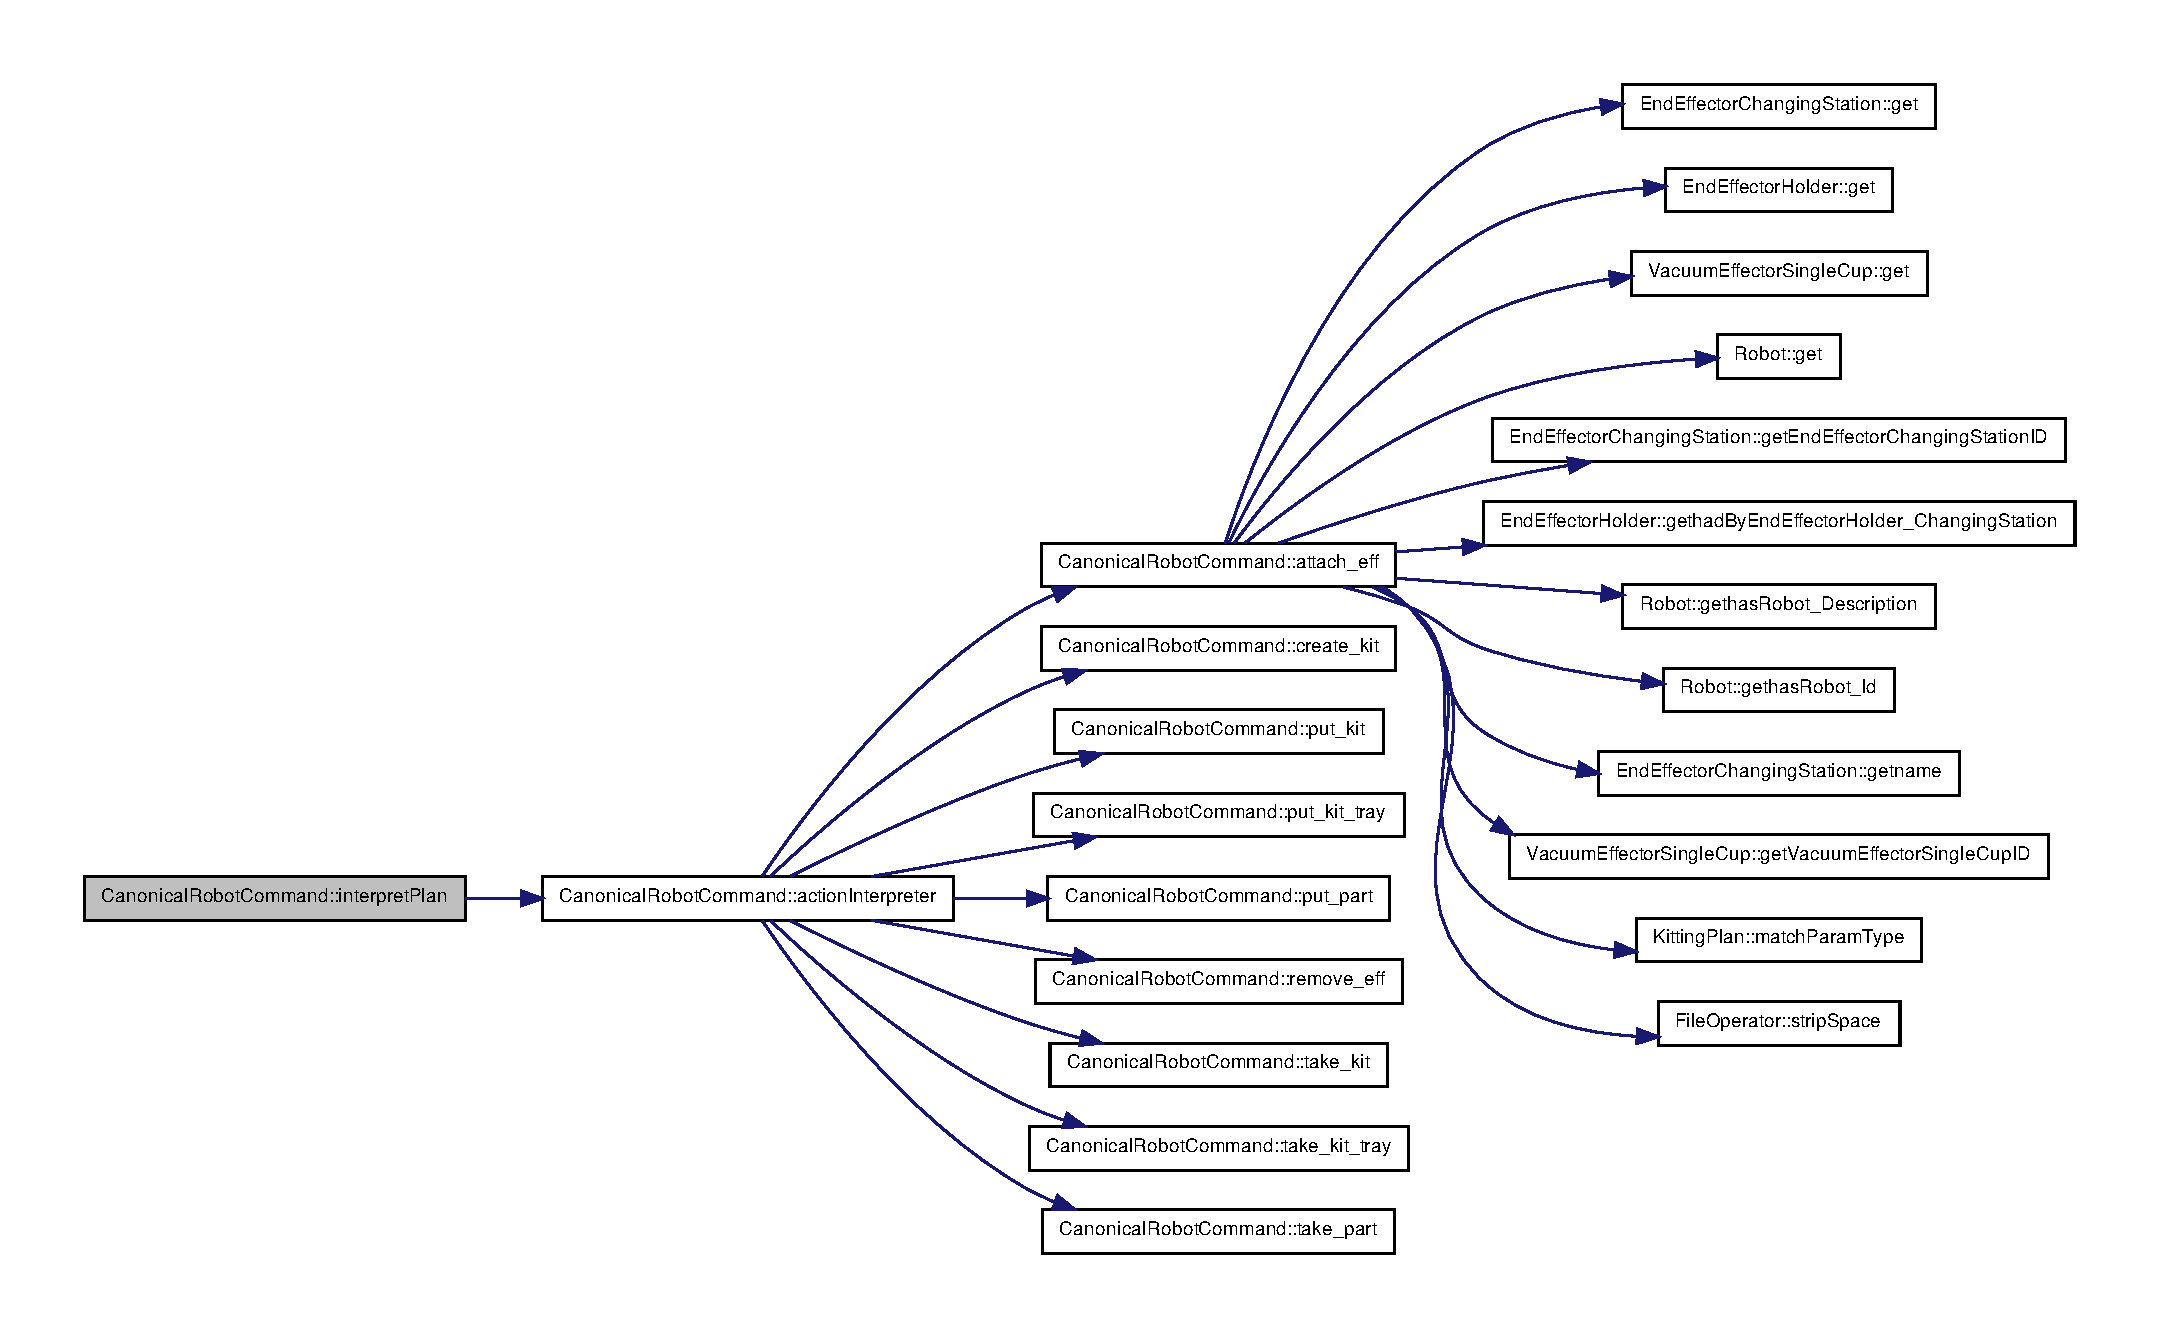
\includegraphics[width=400pt]{class_canonical_robot_command_a8b54b12dc029042eedfa15598f671ac6_cgraph}
\end{center}
\end{figure}




Here is the caller graph for this function:
\nopagebreak
\begin{figure}[H]
\begin{center}
\leavevmode
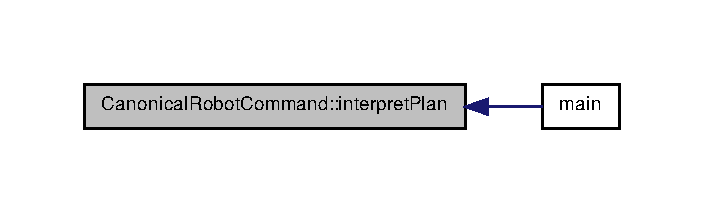
\includegraphics[width=338pt]{class_canonical_robot_command_a8b54b12dc029042eedfa15598f671ac6_icgraph}
\end{center}
\end{figure}


\hypertarget{class_canonical_robot_command_afa48a098e02e9fa34706b251601ca287}{
\index{CanonicalRobotCommand@{CanonicalRobotCommand}!put\_\-kit@{put\_\-kit}}
\index{put\_\-kit@{put\_\-kit}!CanonicalRobotCommand@{CanonicalRobotCommand}}
\subsubsection[{put\_\-kit}]{\setlength{\rightskip}{0pt plus 5cm}void CanonicalRobotCommand::put\_\-kit (
\begin{DoxyParamCaption}
\item[{vector$<$ string $>$}]{paramList}
\end{DoxyParamCaption}
)}}
\label{class_canonical_robot_command_afa48a098e02e9fa34706b251601ca287}


Here is the caller graph for this function:
\nopagebreak
\begin{figure}[H]
\begin{center}
\leavevmode
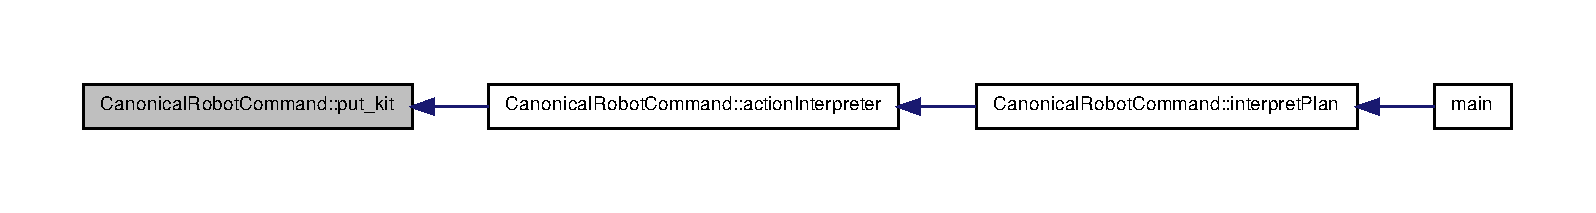
\includegraphics[width=400pt]{class_canonical_robot_command_afa48a098e02e9fa34706b251601ca287_icgraph}
\end{center}
\end{figure}


\hypertarget{class_canonical_robot_command_a5b86751ba4697428c741709d0ac80528}{
\index{CanonicalRobotCommand@{CanonicalRobotCommand}!put\_\-kit\_\-tray@{put\_\-kit\_\-tray}}
\index{put\_\-kit\_\-tray@{put\_\-kit\_\-tray}!CanonicalRobotCommand@{CanonicalRobotCommand}}
\subsubsection[{put\_\-kit\_\-tray}]{\setlength{\rightskip}{0pt plus 5cm}void CanonicalRobotCommand::put\_\-kit\_\-tray (
\begin{DoxyParamCaption}
\item[{vector$<$ string $>$}]{paramList}
\end{DoxyParamCaption}
)}}
\label{class_canonical_robot_command_a5b86751ba4697428c741709d0ac80528}


Here is the caller graph for this function:
\nopagebreak
\begin{figure}[H]
\begin{center}
\leavevmode
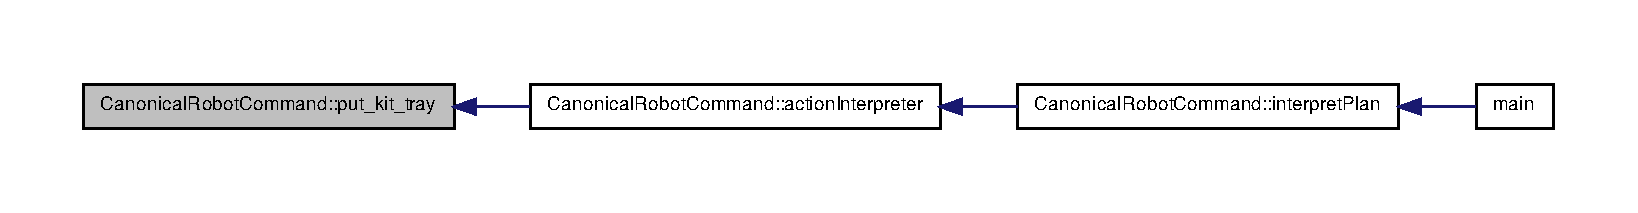
\includegraphics[width=400pt]{class_canonical_robot_command_a5b86751ba4697428c741709d0ac80528_icgraph}
\end{center}
\end{figure}


\hypertarget{class_canonical_robot_command_af366c12a510324c0cd9a5d1ee17476a7}{
\index{CanonicalRobotCommand@{CanonicalRobotCommand}!put\_\-part@{put\_\-part}}
\index{put\_\-part@{put\_\-part}!CanonicalRobotCommand@{CanonicalRobotCommand}}
\subsubsection[{put\_\-part}]{\setlength{\rightskip}{0pt plus 5cm}void CanonicalRobotCommand::put\_\-part (
\begin{DoxyParamCaption}
\item[{vector$<$ string $>$}]{paramList}
\end{DoxyParamCaption}
)}}
\label{class_canonical_robot_command_af366c12a510324c0cd9a5d1ee17476a7}


Here is the caller graph for this function:
\nopagebreak
\begin{figure}[H]
\begin{center}
\leavevmode
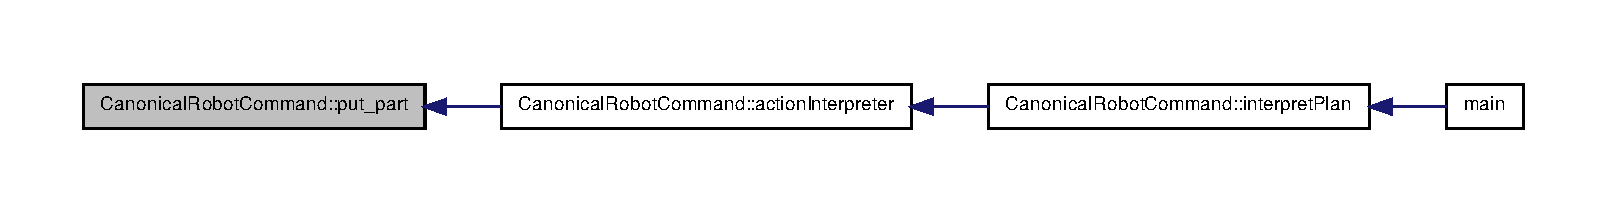
\includegraphics[width=400pt]{class_canonical_robot_command_af366c12a510324c0cd9a5d1ee17476a7_icgraph}
\end{center}
\end{figure}


\hypertarget{class_canonical_robot_command_a6e00f038ab69fb6a6d2f9b3c5882e789}{
\index{CanonicalRobotCommand@{CanonicalRobotCommand}!remove\_\-eff@{remove\_\-eff}}
\index{remove\_\-eff@{remove\_\-eff}!CanonicalRobotCommand@{CanonicalRobotCommand}}
\subsubsection[{remove\_\-eff}]{\setlength{\rightskip}{0pt plus 5cm}void CanonicalRobotCommand::remove\_\-eff (
\begin{DoxyParamCaption}
\item[{vector$<$ string $>$}]{paramList}
\end{DoxyParamCaption}
)}}
\label{class_canonical_robot_command_a6e00f038ab69fb6a6d2f9b3c5882e789}


Here is the caller graph for this function:
\nopagebreak
\begin{figure}[H]
\begin{center}
\leavevmode
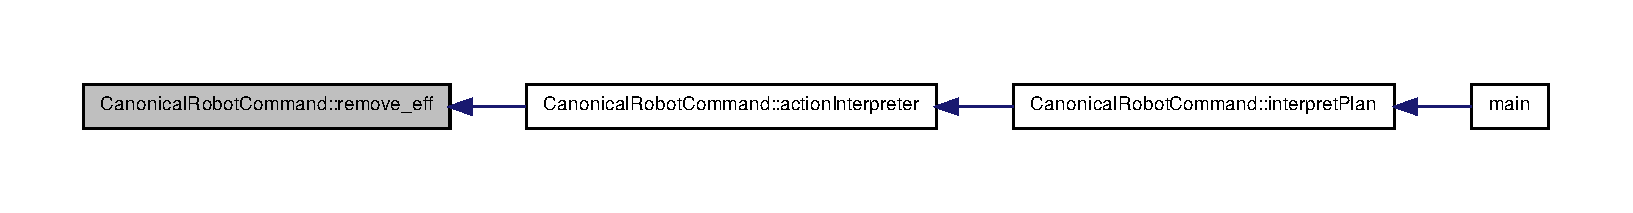
\includegraphics[width=400pt]{class_canonical_robot_command_a6e00f038ab69fb6a6d2f9b3c5882e789_icgraph}
\end{center}
\end{figure}


\hypertarget{class_canonical_robot_command_a33abd5938bb8c1d94bc3616609e418c5}{
\index{CanonicalRobotCommand@{CanonicalRobotCommand}!take\_\-kit@{take\_\-kit}}
\index{take\_\-kit@{take\_\-kit}!CanonicalRobotCommand@{CanonicalRobotCommand}}
\subsubsection[{take\_\-kit}]{\setlength{\rightskip}{0pt plus 5cm}void CanonicalRobotCommand::take\_\-kit (
\begin{DoxyParamCaption}
\item[{vector$<$ string $>$}]{paramList}
\end{DoxyParamCaption}
)}}
\label{class_canonical_robot_command_a33abd5938bb8c1d94bc3616609e418c5}


Here is the caller graph for this function:
\nopagebreak
\begin{figure}[H]
\begin{center}
\leavevmode
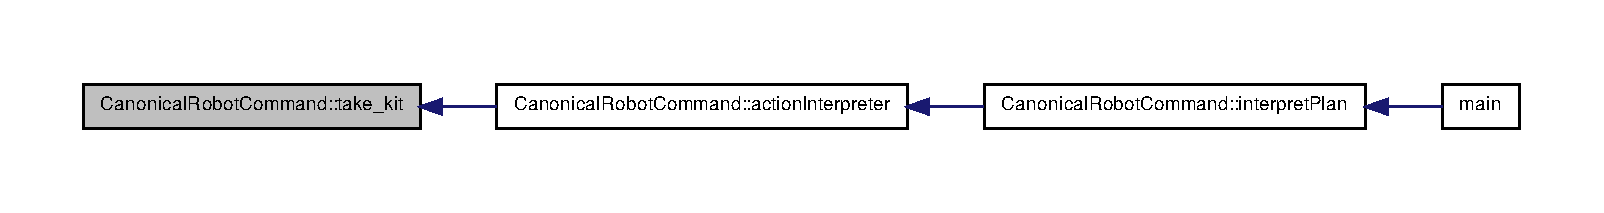
\includegraphics[width=400pt]{class_canonical_robot_command_a33abd5938bb8c1d94bc3616609e418c5_icgraph}
\end{center}
\end{figure}


\hypertarget{class_canonical_robot_command_abc17012640ae9203f090bcdb828c9c0d}{
\index{CanonicalRobotCommand@{CanonicalRobotCommand}!take\_\-kit\_\-tray@{take\_\-kit\_\-tray}}
\index{take\_\-kit\_\-tray@{take\_\-kit\_\-tray}!CanonicalRobotCommand@{CanonicalRobotCommand}}
\subsubsection[{take\_\-kit\_\-tray}]{\setlength{\rightskip}{0pt plus 5cm}void CanonicalRobotCommand::take\_\-kit\_\-tray (
\begin{DoxyParamCaption}
\item[{vector$<$ string $>$}]{paramList}
\end{DoxyParamCaption}
)}}
\label{class_canonical_robot_command_abc17012640ae9203f090bcdb828c9c0d}


Here is the caller graph for this function:
\nopagebreak
\begin{figure}[H]
\begin{center}
\leavevmode
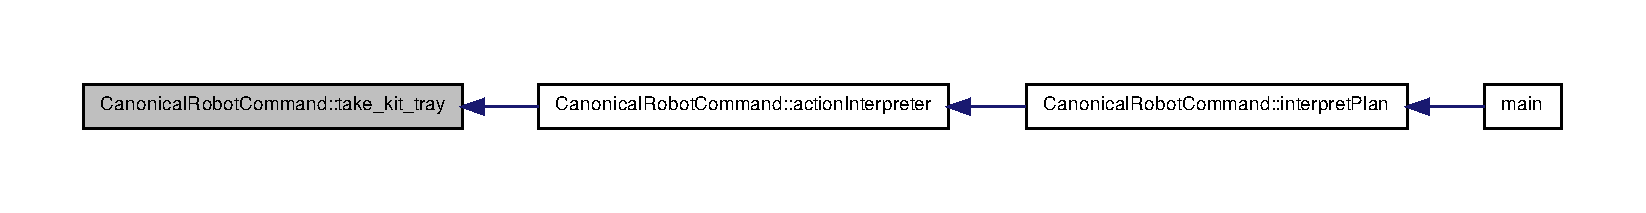
\includegraphics[width=400pt]{class_canonical_robot_command_abc17012640ae9203f090bcdb828c9c0d_icgraph}
\end{center}
\end{figure}


\hypertarget{class_canonical_robot_command_afb89d61a62c1dea47f5abef6b5ec1b4e}{
\index{CanonicalRobotCommand@{CanonicalRobotCommand}!take\_\-part@{take\_\-part}}
\index{take\_\-part@{take\_\-part}!CanonicalRobotCommand@{CanonicalRobotCommand}}
\subsubsection[{take\_\-part}]{\setlength{\rightskip}{0pt plus 5cm}void CanonicalRobotCommand::take\_\-part (
\begin{DoxyParamCaption}
\item[{vector$<$ string $>$}]{paramList}
\end{DoxyParamCaption}
)}}
\label{class_canonical_robot_command_afb89d61a62c1dea47f5abef6b5ec1b4e}


Here is the caller graph for this function:
\nopagebreak
\begin{figure}[H]
\begin{center}
\leavevmode
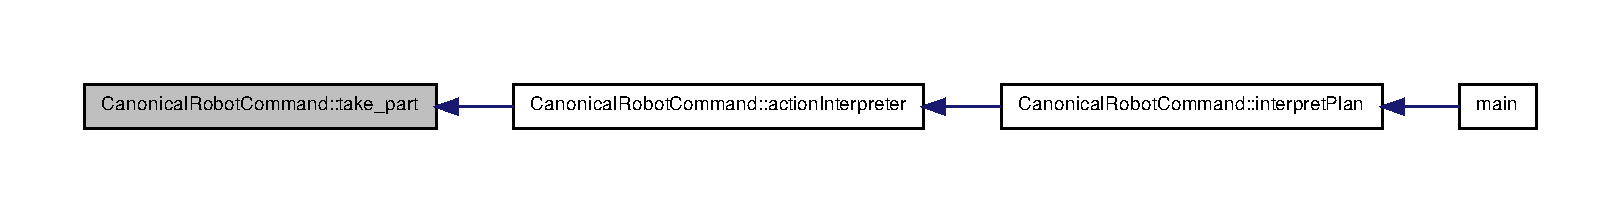
\includegraphics[width=400pt]{class_canonical_robot_command_afb89d61a62c1dea47f5abef6b5ec1b4e_icgraph}
\end{center}
\end{figure}




The documentation for this class was generated from the following files:\begin{DoxyCompactItemize}
\item 
/home/zeid/workspace/executor/src/interpreter/\hyperlink{_canonical_robot_command_8h}{CanonicalRobotCommand.h}\item 
/home/zeid/workspace/executor/src/interpreter/\hyperlink{_canonical_robot_command_8cc}{CanonicalRobotCommand.cc}\end{DoxyCompactItemize}

\hypertarget{class_close_gripper_msg}{
\section{CloseGripperMsg Class Reference}
\label{class_close_gripper_msg}\index{CloseGripperMsg@{CloseGripperMsg}}
}


{\ttfamily \#include $<$canonicalMsg.hh$>$}



Inheritance diagram for CloseGripperMsg:\nopagebreak
\begin{figure}[H]
\begin{center}
\leavevmode
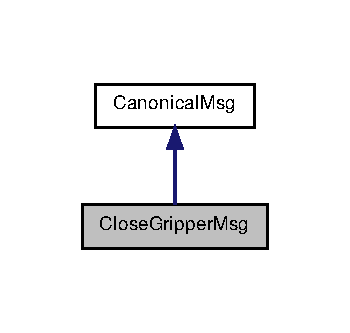
\includegraphics[width=168pt]{class_close_gripper_msg__inherit__graph}
\end{center}
\end{figure}


Collaboration diagram for CloseGripperMsg:\nopagebreak
\begin{figure}[H]
\begin{center}
\leavevmode
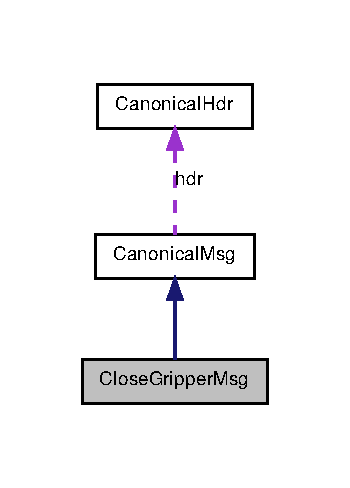
\includegraphics[width=168pt]{class_close_gripper_msg__coll__graph}
\end{center}
\end{figure}
\subsection*{Public Member Functions}
\begin{DoxyCompactItemize}
\item 
\hyperlink{class_close_gripper_msg_a6a9dab1776907abd3a9d5e4d82c8946d}{CloseGripperMsg} ()
\item 
\hyperlink{class_close_gripper_msg_a3509d8bb099aa32b1d2d8072c291a1b5}{$\sim$CloseGripperMsg} ()
\end{DoxyCompactItemize}


\subsection{Constructor \& Destructor Documentation}
\hypertarget{class_close_gripper_msg_a6a9dab1776907abd3a9d5e4d82c8946d}{
\index{CloseGripperMsg@{CloseGripperMsg}!CloseGripperMsg@{CloseGripperMsg}}
\index{CloseGripperMsg@{CloseGripperMsg}!CloseGripperMsg@{CloseGripperMsg}}
\subsubsection[{CloseGripperMsg}]{\setlength{\rightskip}{0pt plus 5cm}CloseGripperMsg::CloseGripperMsg (
\begin{DoxyParamCaption}
{}
\end{DoxyParamCaption}
)\hspace{0.3cm}{\ttfamily  \mbox{[}inline\mbox{]}}}}
\label{class_close_gripper_msg_a6a9dab1776907abd3a9d5e4d82c8946d}
\hypertarget{class_close_gripper_msg_a3509d8bb099aa32b1d2d8072c291a1b5}{
\index{CloseGripperMsg@{CloseGripperMsg}!$\sim$CloseGripperMsg@{$\sim$CloseGripperMsg}}
\index{$\sim$CloseGripperMsg@{$\sim$CloseGripperMsg}!CloseGripperMsg@{CloseGripperMsg}}
\subsubsection[{$\sim$CloseGripperMsg}]{\setlength{\rightskip}{0pt plus 5cm}CloseGripperMsg::$\sim$CloseGripperMsg (
\begin{DoxyParamCaption}
{}
\end{DoxyParamCaption}
)\hspace{0.3cm}{\ttfamily  \mbox{[}inline\mbox{]}}}}
\label{class_close_gripper_msg_a3509d8bb099aa32b1d2d8072c291a1b5}


The documentation for this class was generated from the following file:\begin{DoxyCompactItemize}
\item 
/home/zeid/workspace/executor/src/controller/\hyperlink{canonical_msg_8hh}{canonicalMsg.hh}\end{DoxyCompactItemize}

\hypertarget{class_connection}{
\section{Connection Class Reference}
\label{class_connection}\index{Connection@{Connection}}
}


{\ttfamily \#include $<$Connection.h$>$}

\subsection*{Public Member Functions}
\begin{DoxyCompactItemize}
\item 
\hyperlink{class_connection_a6970de2fa9268fe6f96179f62896ebb1}{Connection} (std::string url, std::string user, std::string pass, std::string name)
\item 
virtual \hyperlink{class_connection_a2e4352edf667bea83001569e9da8a24d}{$\sim$Connection} ()
\item 
sql::Connection $\ast$ \hyperlink{class_connection_a1a452e7d0205cbf773855fe7721a52dd}{getCon} () const 
\item 
sql::mysql::MySQL\_\-Driver $\ast$ \hyperlink{class_connection_aab4ca656dabf965911a04e1df739b2d5}{getDriver} () const 
\item 
void \hyperlink{class_connection_a83036b70adab4586a8daba905b4e3cd6}{setCon} (sql::Connection $\ast$con)
\item 
void \hyperlink{class_connection_af98d381ac53362ffa8661c40d0ab3b13}{setDriver} (sql::mysql::MySQL\_\-Driver $\ast$driver)
\end{DoxyCompactItemize}


\subsection{Constructor \& Destructor Documentation}
\hypertarget{class_connection_a6970de2fa9268fe6f96179f62896ebb1}{
\index{Connection@{Connection}!Connection@{Connection}}
\index{Connection@{Connection}!Connection@{Connection}}
\subsubsection[{Connection}]{\setlength{\rightskip}{0pt plus 5cm}Connection::Connection (
\begin{DoxyParamCaption}
\item[{std::string}]{url, }
\item[{std::string}]{user, }
\item[{std::string}]{pass, }
\item[{std::string}]{name}
\end{DoxyParamCaption}
)}}
\label{class_connection_a6970de2fa9268fe6f96179f62896ebb1}
\hypertarget{class_connection_a2e4352edf667bea83001569e9da8a24d}{
\index{Connection@{Connection}!$\sim$Connection@{$\sim$Connection}}
\index{$\sim$Connection@{$\sim$Connection}!Connection@{Connection}}
\subsubsection[{$\sim$Connection}]{\setlength{\rightskip}{0pt plus 5cm}Connection::$\sim$Connection (
\begin{DoxyParamCaption}
{}
\end{DoxyParamCaption}
)\hspace{0.3cm}{\ttfamily  \mbox{[}virtual\mbox{]}}}}
\label{class_connection_a2e4352edf667bea83001569e9da8a24d}


\subsection{Member Function Documentation}
\hypertarget{class_connection_a1a452e7d0205cbf773855fe7721a52dd}{
\index{Connection@{Connection}!getCon@{getCon}}
\index{getCon@{getCon}!Connection@{Connection}}
\subsubsection[{getCon}]{\setlength{\rightskip}{0pt plus 5cm}sql::Connection $\ast$ Connection::getCon (
\begin{DoxyParamCaption}
{}
\end{DoxyParamCaption}
) const}}
\label{class_connection_a1a452e7d0205cbf773855fe7721a52dd}


Here is the caller graph for this function:\nopagebreak
\begin{figure}[H]
\begin{center}
\leavevmode
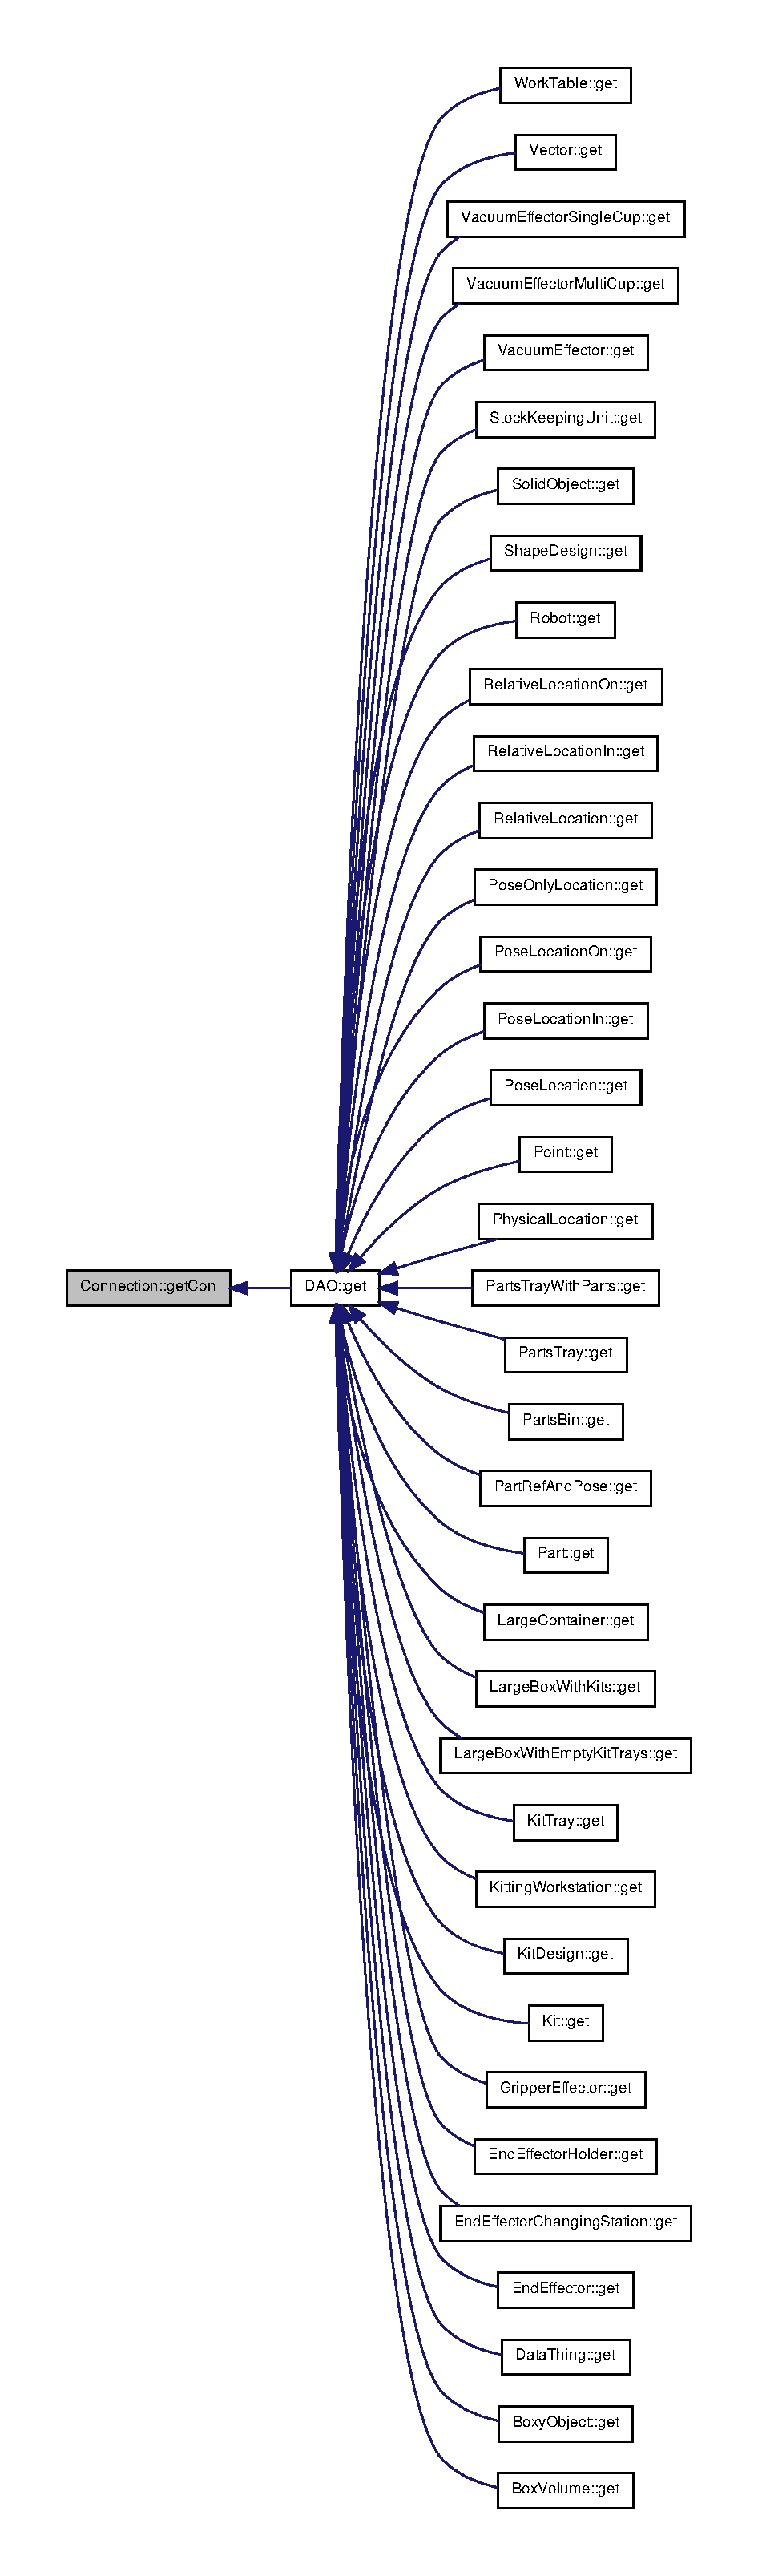
\includegraphics[height=600pt]{class_connection_a1a452e7d0205cbf773855fe7721a52dd_icgraph}
\end{center}
\end{figure}


\hypertarget{class_connection_aab4ca656dabf965911a04e1df739b2d5}{
\index{Connection@{Connection}!getDriver@{getDriver}}
\index{getDriver@{getDriver}!Connection@{Connection}}
\subsubsection[{getDriver}]{\setlength{\rightskip}{0pt plus 5cm}sql::mysql::MySQL\_\-Driver $\ast$ Connection::getDriver (
\begin{DoxyParamCaption}
{}
\end{DoxyParamCaption}
) const}}
\label{class_connection_aab4ca656dabf965911a04e1df739b2d5}
\hypertarget{class_connection_a83036b70adab4586a8daba905b4e3cd6}{
\index{Connection@{Connection}!setCon@{setCon}}
\index{setCon@{setCon}!Connection@{Connection}}
\subsubsection[{setCon}]{\setlength{\rightskip}{0pt plus 5cm}void Connection::setCon (
\begin{DoxyParamCaption}
\item[{sql::Connection $\ast$}]{con}
\end{DoxyParamCaption}
)}}
\label{class_connection_a83036b70adab4586a8daba905b4e3cd6}
\hypertarget{class_connection_af98d381ac53362ffa8661c40d0ab3b13}{
\index{Connection@{Connection}!setDriver@{setDriver}}
\index{setDriver@{setDriver}!Connection@{Connection}}
\subsubsection[{setDriver}]{\setlength{\rightskip}{0pt plus 5cm}void Connection::setDriver (
\begin{DoxyParamCaption}
\item[{sql::mysql::MySQL\_\-Driver $\ast$}]{driver}
\end{DoxyParamCaption}
)}}
\label{class_connection_af98d381ac53362ffa8661c40d0ab3b13}


The documentation for this class was generated from the following files:\begin{DoxyCompactItemize}
\item 
/home/zeid/workspace/executor/src/database/\hyperlink{_connection_8h}{Connection.h}\item 
/home/zeid/workspace/executor/src/database/\hyperlink{_connection_8cpp}{Connection.cpp}\end{DoxyCompactItemize}

\hypertarget{class_controller}{
\section{Controller Class Reference}
\label{class_controller}\index{Controller@{Controller}}
}


{\ttfamily \#include $<$controller.hh$>$}



Inheritance diagram for Controller:\nopagebreak
\begin{figure}[H]
\begin{center}
\leavevmode
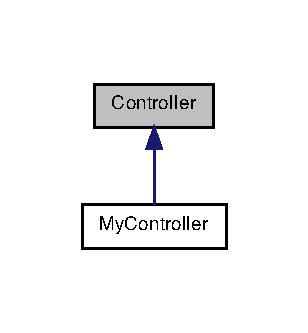
\includegraphics[width=148pt]{class_controller__inherit__graph}
\end{center}
\end{figure}
\subsection*{Public Member Functions}
\begin{DoxyCompactItemize}
\item 
\hyperlink{class_controller_a95c56822d667e94b031451729ce069a9}{Controller} ()
\item 
\hyperlink{class_controller_a0ab87934c4f7a266cfdb86e0f36bc1b5}{$\sim$Controller} ()
\item 
int \hyperlink{class_controller_a45d996d1abb23d8e84edb35d04c5870f}{queueMsg} (\hyperlink{class_canonical_msg}{CanonicalMsg} $\ast$msgIn)
\item 
int \hyperlink{class_controller_a6b15d05b97d71db389603e91f0b344d0}{queueCloseGripper} (\hyperlink{class_close_gripper_msg}{CloseGripperMsg} closeGripperMsg)
\item 
int \hyperlink{class_controller_ad8bf10b2328e182033cd04ac6e0d8c9a}{queueDwell} (\hyperlink{class_dwell_msg}{DwellMsg} dwellMsg)
\item 
int \hyperlink{class_controller_a365bdbaf661a5c4328240f8f8838400d}{dequeueMsg} ()
\item 
virtual int \hyperlink{class_controller_a5ec3a5ed8ac04038cd0a2afe19e9e797}{processCloseGripper} (\hyperlink{class_close_gripper_msg}{CloseGripperMsg} $\ast$closeGripperMsg)=0
\item 
virtual int \hyperlink{class_controller_ae692153a067c9893d00ab3a13392c653}{processDwell} (\hyperlink{class_dwell_msg}{DwellMsg} $\ast$dwellMsg)=0
\item 
virtual int \hyperlink{class_controller_a06f7f8733ae96e812cb17b03faffe893}{processEndCanon} (\hyperlink{class_end_canon_msg}{EndCanonMsg} $\ast$endCanonMsg)=0
\item 
virtual int \hyperlink{class_controller_ad38c7457a8d09653baadff8d70df03b8}{processInitCanon} (\hyperlink{class_init_canon_msg}{InitCanonMsg} $\ast$initCanonMsg)=0
\item 
virtual int \hyperlink{class_controller_a93ff1647ac9341d8852f4017f98a6722}{processMessage} (\hyperlink{class_message_msg}{MessageMsg} $\ast$messageMsg)=0
\item 
virtual int \hyperlink{class_controller_a835d9f06bbdb8d23fa5969a3007c5dbc}{processMoveSmoothlyTo} (\hyperlink{class_move_smoothly_to_msg}{MoveSmoothlyToMsg} $\ast$moveSmoothlyToMsg)=0
\item 
virtual int \hyperlink{class_controller_a95e1b3c824aff33ffa6775b1eca4b4ee}{processMoveStraightTo} (\hyperlink{class_move_straight_to_msg}{MoveStraightToMsg} $\ast$moveStraightToMsg)=0
\item 
virtual int \hyperlink{class_controller_ac5cf7c0b8dd2425a4a1d2a374a4db757}{processMoveTo} (\hyperlink{class_move_to_msg}{MoveToMsg} $\ast$moveToMsg)=0
\item 
virtual int \hyperlink{class_controller_af6c4c75d0d89983475c0dda414b4a4f1}{processOpenGripper} (\hyperlink{class_open_gripper_msg}{OpenGripperMsg} $\ast$openGripperMsg)=0
\item 
virtual int \hyperlink{class_controller_a2bcd07407b259343dbf12a457505946d}{processSetAbsoluteAcceleration} (\hyperlink{class_set_absolute_acceleration_msg}{SetAbsoluteAccelerationMsg} $\ast$setAbsoluteAccelerationMsg)=0
\item 
virtual int \hyperlink{class_controller_a80daac4509d5936f966e5289528e2b7c}{processSetAngleUnits} (\hyperlink{class_set_angle_units_msg}{SetAngleUnitsMsg} $\ast$setAngleUnitsMsg)=0
\item 
virtual int \hyperlink{class_controller_a698966c052faebede44e65a0b2b16493}{processSetEndAngleTolerance} (\hyperlink{class_set_end_angle_tolerance_msg}{SetEndAngleToleranceMsg} $\ast$setEndAngleToleranceMsg)=0
\item 
virtual int \hyperlink{class_controller_a5a8fc3403231a34be7f4a6426c6c1954}{processSetEndPointTolerance} (\hyperlink{class_set_end_point_tolerance_msg}{SetEndPointToleranceMsg} $\ast$setEndPointToleranceMsg)=0
\item 
virtual int \hyperlink{class_controller_a1a3cf77b97ccce4a364f556118ea3eb0}{processSetIntermediatePointTolerance} (\hyperlink{class_set_intermediate_point_tolerance_msg}{SetIntermediatePointToleranceMsg} $\ast$setIntermediatePointToleranceMsg)=0
\item 
virtual int \hyperlink{class_controller_a2158164839e7019556d4785528fc5874}{processSetLengthUnits} (\hyperlink{class_set_length_units_msg}{SetLengthUnitsMsg} $\ast$setLengthUnitsMsg)=0
\item 
virtual int \hyperlink{class_controller_a977a24df59729a6f795ea179af3d05a4}{processSetRelativeAcceleration} (\hyperlink{class_set_relative_acceleration_msg}{SetRelativeAccelerationMsg} $\ast$setRelativeAccelerationMsg)=0
\item 
virtual int \hyperlink{class_controller_a25229410c00d8baf4fa2fde5fa7549c0}{processSetRelativeSpeed} (\hyperlink{class_set_relative_speed_msg}{SetRelativeSpeedMsg} $\ast$setRelativeSpeedMsg)=0
\end{DoxyCompactItemize}


\subsection{Constructor \& Destructor Documentation}
\hypertarget{class_controller_a95c56822d667e94b031451729ce069a9}{
\index{Controller@{Controller}!Controller@{Controller}}
\index{Controller@{Controller}!Controller@{Controller}}
\subsubsection[{Controller}]{\setlength{\rightskip}{0pt plus 5cm}Controller::Controller (
\begin{DoxyParamCaption}
{}
\end{DoxyParamCaption}
)}}
\label{class_controller_a95c56822d667e94b031451729ce069a9}
\hypertarget{class_controller_a0ab87934c4f7a266cfdb86e0f36bc1b5}{
\index{Controller@{Controller}!$\sim$Controller@{$\sim$Controller}}
\index{$\sim$Controller@{$\sim$Controller}!Controller@{Controller}}
\subsubsection[{$\sim$Controller}]{\setlength{\rightskip}{0pt plus 5cm}Controller::$\sim$Controller (
\begin{DoxyParamCaption}
{}
\end{DoxyParamCaption}
)}}
\label{class_controller_a0ab87934c4f7a266cfdb86e0f36bc1b5}


\subsection{Member Function Documentation}
\hypertarget{class_controller_a365bdbaf661a5c4328240f8f8838400d}{
\index{Controller@{Controller}!dequeueMsg@{dequeueMsg}}
\index{dequeueMsg@{dequeueMsg}!Controller@{Controller}}
\subsubsection[{dequeueMsg}]{\setlength{\rightskip}{0pt plus 5cm}int Controller::dequeueMsg (
\begin{DoxyParamCaption}
{}
\end{DoxyParamCaption}
)}}
\label{class_controller_a365bdbaf661a5c4328240f8f8838400d}


Here is the call graph for this function:\nopagebreak
\begin{figure}[H]
\begin{center}
\leavevmode
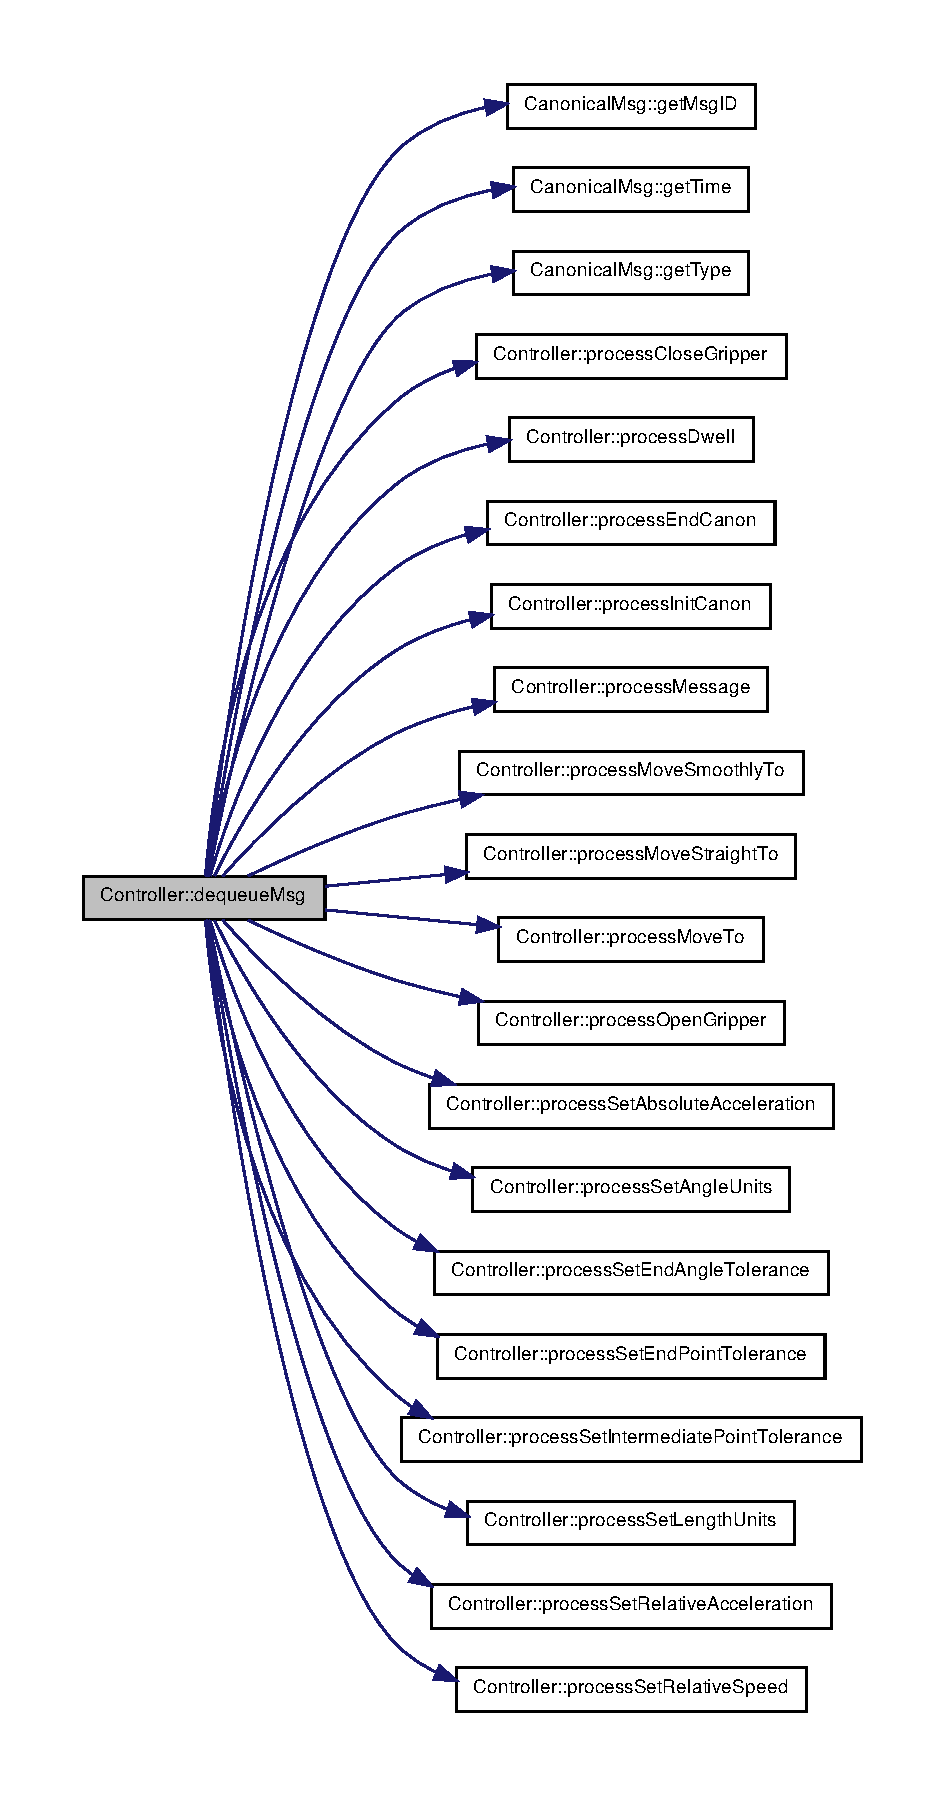
\includegraphics[height=600pt]{class_controller_a365bdbaf661a5c4328240f8f8838400d_cgraph}
\end{center}
\end{figure}


\hypertarget{class_controller_a5ec3a5ed8ac04038cd0a2afe19e9e797}{
\index{Controller@{Controller}!processCloseGripper@{processCloseGripper}}
\index{processCloseGripper@{processCloseGripper}!Controller@{Controller}}
\subsubsection[{processCloseGripper}]{\setlength{\rightskip}{0pt plus 5cm}virtual int Controller::processCloseGripper (
\begin{DoxyParamCaption}
\item[{{\bf CloseGripperMsg} $\ast$}]{closeGripperMsg}
\end{DoxyParamCaption}
)\hspace{0.3cm}{\ttfamily  \mbox{[}pure virtual\mbox{]}}}}
\label{class_controller_a5ec3a5ed8ac04038cd0a2afe19e9e797}


Implemented in \hyperlink{class_my_controller_afcd5a91653e0c6035274e0d2b287d9ff}{MyController}.



Here is the caller graph for this function:\nopagebreak
\begin{figure}[H]
\begin{center}
\leavevmode
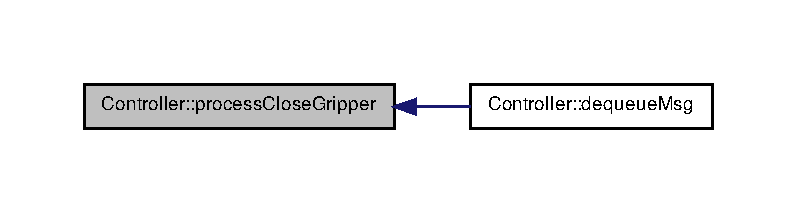
\includegraphics[width=382pt]{class_controller_a5ec3a5ed8ac04038cd0a2afe19e9e797_icgraph}
\end{center}
\end{figure}


\hypertarget{class_controller_ae692153a067c9893d00ab3a13392c653}{
\index{Controller@{Controller}!processDwell@{processDwell}}
\index{processDwell@{processDwell}!Controller@{Controller}}
\subsubsection[{processDwell}]{\setlength{\rightskip}{0pt plus 5cm}virtual int Controller::processDwell (
\begin{DoxyParamCaption}
\item[{{\bf DwellMsg} $\ast$}]{dwellMsg}
\end{DoxyParamCaption}
)\hspace{0.3cm}{\ttfamily  \mbox{[}pure virtual\mbox{]}}}}
\label{class_controller_ae692153a067c9893d00ab3a13392c653}


Implemented in \hyperlink{class_my_controller_a4e5f21b2e983f04cbb239b125b3b117e}{MyController}.



Here is the caller graph for this function:\nopagebreak
\begin{figure}[H]
\begin{center}
\leavevmode
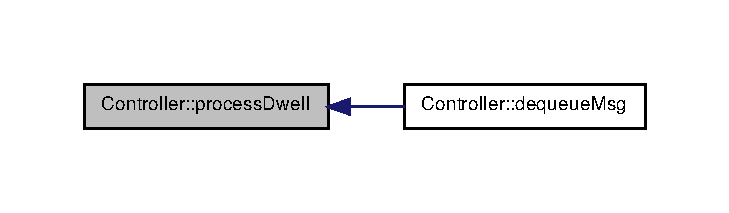
\includegraphics[width=350pt]{class_controller_ae692153a067c9893d00ab3a13392c653_icgraph}
\end{center}
\end{figure}


\hypertarget{class_controller_a06f7f8733ae96e812cb17b03faffe893}{
\index{Controller@{Controller}!processEndCanon@{processEndCanon}}
\index{processEndCanon@{processEndCanon}!Controller@{Controller}}
\subsubsection[{processEndCanon}]{\setlength{\rightskip}{0pt plus 5cm}virtual int Controller::processEndCanon (
\begin{DoxyParamCaption}
\item[{{\bf EndCanonMsg} $\ast$}]{endCanonMsg}
\end{DoxyParamCaption}
)\hspace{0.3cm}{\ttfamily  \mbox{[}pure virtual\mbox{]}}}}
\label{class_controller_a06f7f8733ae96e812cb17b03faffe893}


Implemented in \hyperlink{class_my_controller_a2d89a8878736628f6be3cb228f10e5d0}{MyController}.



Here is the caller graph for this function:\nopagebreak
\begin{figure}[H]
\begin{center}
\leavevmode
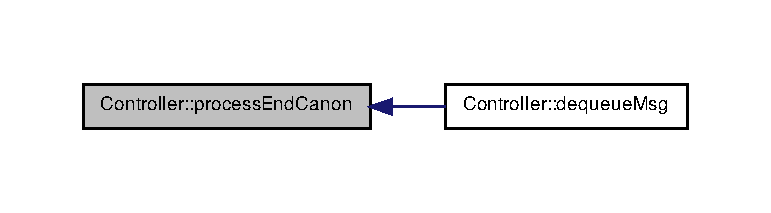
\includegraphics[width=370pt]{class_controller_a06f7f8733ae96e812cb17b03faffe893_icgraph}
\end{center}
\end{figure}


\hypertarget{class_controller_ad38c7457a8d09653baadff8d70df03b8}{
\index{Controller@{Controller}!processInitCanon@{processInitCanon}}
\index{processInitCanon@{processInitCanon}!Controller@{Controller}}
\subsubsection[{processInitCanon}]{\setlength{\rightskip}{0pt plus 5cm}virtual int Controller::processInitCanon (
\begin{DoxyParamCaption}
\item[{{\bf InitCanonMsg} $\ast$}]{initCanonMsg}
\end{DoxyParamCaption}
)\hspace{0.3cm}{\ttfamily  \mbox{[}pure virtual\mbox{]}}}}
\label{class_controller_ad38c7457a8d09653baadff8d70df03b8}


Implemented in \hyperlink{class_my_controller_abc8fd5a12f022e6b9b38351326d9be50}{MyController}.



Here is the caller graph for this function:\nopagebreak
\begin{figure}[H]
\begin{center}
\leavevmode
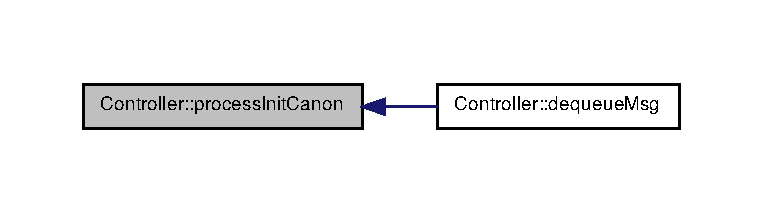
\includegraphics[width=366pt]{class_controller_ad38c7457a8d09653baadff8d70df03b8_icgraph}
\end{center}
\end{figure}


\hypertarget{class_controller_a93ff1647ac9341d8852f4017f98a6722}{
\index{Controller@{Controller}!processMessage@{processMessage}}
\index{processMessage@{processMessage}!Controller@{Controller}}
\subsubsection[{processMessage}]{\setlength{\rightskip}{0pt plus 5cm}virtual int Controller::processMessage (
\begin{DoxyParamCaption}
\item[{{\bf MessageMsg} $\ast$}]{messageMsg}
\end{DoxyParamCaption}
)\hspace{0.3cm}{\ttfamily  \mbox{[}pure virtual\mbox{]}}}}
\label{class_controller_a93ff1647ac9341d8852f4017f98a6722}


Implemented in \hyperlink{class_my_controller_aee5bcc193cb15db025c2023df3ad04d6}{MyController}.



Here is the caller graph for this function:\nopagebreak
\begin{figure}[H]
\begin{center}
\leavevmode
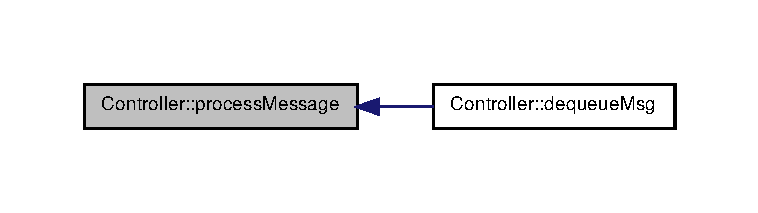
\includegraphics[width=364pt]{class_controller_a93ff1647ac9341d8852f4017f98a6722_icgraph}
\end{center}
\end{figure}


\hypertarget{class_controller_a835d9f06bbdb8d23fa5969a3007c5dbc}{
\index{Controller@{Controller}!processMoveSmoothlyTo@{processMoveSmoothlyTo}}
\index{processMoveSmoothlyTo@{processMoveSmoothlyTo}!Controller@{Controller}}
\subsubsection[{processMoveSmoothlyTo}]{\setlength{\rightskip}{0pt plus 5cm}virtual int Controller::processMoveSmoothlyTo (
\begin{DoxyParamCaption}
\item[{{\bf MoveSmoothlyToMsg} $\ast$}]{moveSmoothlyToMsg}
\end{DoxyParamCaption}
)\hspace{0.3cm}{\ttfamily  \mbox{[}pure virtual\mbox{]}}}}
\label{class_controller_a835d9f06bbdb8d23fa5969a3007c5dbc}


Implemented in \hyperlink{class_my_controller_af772f22c2df0e5cf2a88fb517ce849e5}{MyController}.



Here is the caller graph for this function:\nopagebreak
\begin{figure}[H]
\begin{center}
\leavevmode
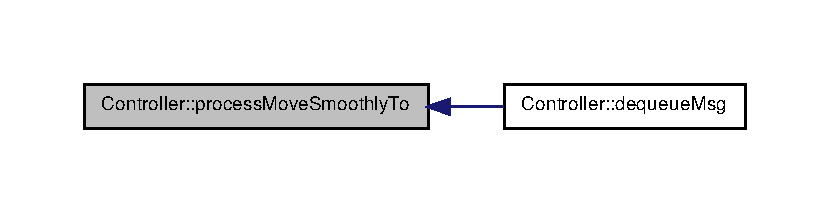
\includegraphics[width=398pt]{class_controller_a835d9f06bbdb8d23fa5969a3007c5dbc_icgraph}
\end{center}
\end{figure}


\hypertarget{class_controller_a95e1b3c824aff33ffa6775b1eca4b4ee}{
\index{Controller@{Controller}!processMoveStraightTo@{processMoveStraightTo}}
\index{processMoveStraightTo@{processMoveStraightTo}!Controller@{Controller}}
\subsubsection[{processMoveStraightTo}]{\setlength{\rightskip}{0pt plus 5cm}virtual int Controller::processMoveStraightTo (
\begin{DoxyParamCaption}
\item[{{\bf MoveStraightToMsg} $\ast$}]{moveStraightToMsg}
\end{DoxyParamCaption}
)\hspace{0.3cm}{\ttfamily  \mbox{[}pure virtual\mbox{]}}}}
\label{class_controller_a95e1b3c824aff33ffa6775b1eca4b4ee}


Implemented in \hyperlink{class_my_controller_a78051383c5b6fa4215af42f243f74a85}{MyController}.



Here is the caller graph for this function:\nopagebreak
\begin{figure}[H]
\begin{center}
\leavevmode
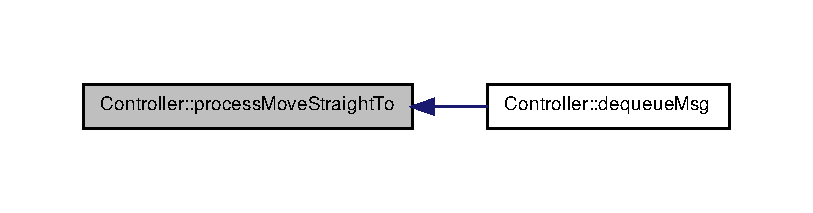
\includegraphics[width=390pt]{class_controller_a95e1b3c824aff33ffa6775b1eca4b4ee_icgraph}
\end{center}
\end{figure}


\hypertarget{class_controller_ac5cf7c0b8dd2425a4a1d2a374a4db757}{
\index{Controller@{Controller}!processMoveTo@{processMoveTo}}
\index{processMoveTo@{processMoveTo}!Controller@{Controller}}
\subsubsection[{processMoveTo}]{\setlength{\rightskip}{0pt plus 5cm}virtual int Controller::processMoveTo (
\begin{DoxyParamCaption}
\item[{{\bf MoveToMsg} $\ast$}]{moveToMsg}
\end{DoxyParamCaption}
)\hspace{0.3cm}{\ttfamily  \mbox{[}pure virtual\mbox{]}}}}
\label{class_controller_ac5cf7c0b8dd2425a4a1d2a374a4db757}


Implemented in \hyperlink{class_my_controller_ac1b346b099111f8be0cc87de1be77257}{MyController}.



Here is the caller graph for this function:\nopagebreak
\begin{figure}[H]
\begin{center}
\leavevmode
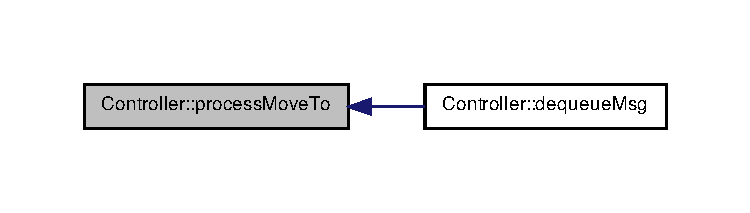
\includegraphics[width=360pt]{class_controller_ac5cf7c0b8dd2425a4a1d2a374a4db757_icgraph}
\end{center}
\end{figure}


\hypertarget{class_controller_af6c4c75d0d89983475c0dda414b4a4f1}{
\index{Controller@{Controller}!processOpenGripper@{processOpenGripper}}
\index{processOpenGripper@{processOpenGripper}!Controller@{Controller}}
\subsubsection[{processOpenGripper}]{\setlength{\rightskip}{0pt plus 5cm}virtual int Controller::processOpenGripper (
\begin{DoxyParamCaption}
\item[{{\bf OpenGripperMsg} $\ast$}]{openGripperMsg}
\end{DoxyParamCaption}
)\hspace{0.3cm}{\ttfamily  \mbox{[}pure virtual\mbox{]}}}}
\label{class_controller_af6c4c75d0d89983475c0dda414b4a4f1}


Implemented in \hyperlink{class_my_controller_a696619700ae953876061cc93dff95973}{MyController}.



Here is the caller graph for this function:\nopagebreak
\begin{figure}[H]
\begin{center}
\leavevmode
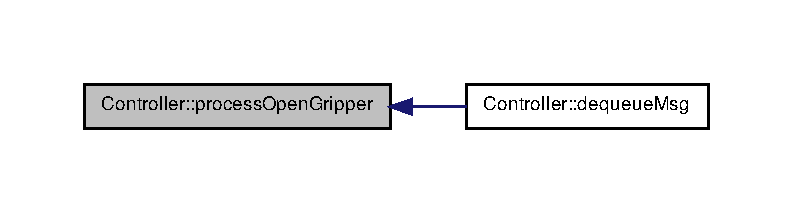
\includegraphics[width=380pt]{class_controller_af6c4c75d0d89983475c0dda414b4a4f1_icgraph}
\end{center}
\end{figure}


\hypertarget{class_controller_a2bcd07407b259343dbf12a457505946d}{
\index{Controller@{Controller}!processSetAbsoluteAcceleration@{processSetAbsoluteAcceleration}}
\index{processSetAbsoluteAcceleration@{processSetAbsoluteAcceleration}!Controller@{Controller}}
\subsubsection[{processSetAbsoluteAcceleration}]{\setlength{\rightskip}{0pt plus 5cm}virtual int Controller::processSetAbsoluteAcceleration (
\begin{DoxyParamCaption}
\item[{{\bf SetAbsoluteAccelerationMsg} $\ast$}]{setAbsoluteAccelerationMsg}
\end{DoxyParamCaption}
)\hspace{0.3cm}{\ttfamily  \mbox{[}pure virtual\mbox{]}}}}
\label{class_controller_a2bcd07407b259343dbf12a457505946d}


Implemented in \hyperlink{class_my_controller_a71f8c98b796a6905e3258e8505ba9e4d}{MyController}.



Here is the caller graph for this function:\nopagebreak
\begin{figure}[H]
\begin{center}
\leavevmode
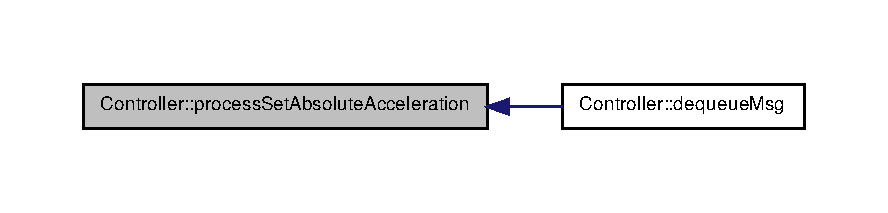
\includegraphics[width=400pt]{class_controller_a2bcd07407b259343dbf12a457505946d_icgraph}
\end{center}
\end{figure}


\hypertarget{class_controller_a80daac4509d5936f966e5289528e2b7c}{
\index{Controller@{Controller}!processSetAngleUnits@{processSetAngleUnits}}
\index{processSetAngleUnits@{processSetAngleUnits}!Controller@{Controller}}
\subsubsection[{processSetAngleUnits}]{\setlength{\rightskip}{0pt plus 5cm}virtual int Controller::processSetAngleUnits (
\begin{DoxyParamCaption}
\item[{{\bf SetAngleUnitsMsg} $\ast$}]{setAngleUnitsMsg}
\end{DoxyParamCaption}
)\hspace{0.3cm}{\ttfamily  \mbox{[}pure virtual\mbox{]}}}}
\label{class_controller_a80daac4509d5936f966e5289528e2b7c}


Implemented in \hyperlink{class_my_controller_a171f022e207b9155be4b1a7a6c824943}{MyController}.



Here is the caller graph for this function:\nopagebreak
\begin{figure}[H]
\begin{center}
\leavevmode
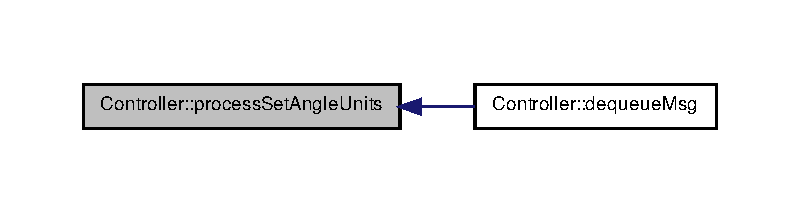
\includegraphics[width=384pt]{class_controller_a80daac4509d5936f966e5289528e2b7c_icgraph}
\end{center}
\end{figure}


\hypertarget{class_controller_a698966c052faebede44e65a0b2b16493}{
\index{Controller@{Controller}!processSetEndAngleTolerance@{processSetEndAngleTolerance}}
\index{processSetEndAngleTolerance@{processSetEndAngleTolerance}!Controller@{Controller}}
\subsubsection[{processSetEndAngleTolerance}]{\setlength{\rightskip}{0pt plus 5cm}virtual int Controller::processSetEndAngleTolerance (
\begin{DoxyParamCaption}
\item[{{\bf SetEndAngleToleranceMsg} $\ast$}]{setEndAngleToleranceMsg}
\end{DoxyParamCaption}
)\hspace{0.3cm}{\ttfamily  \mbox{[}pure virtual\mbox{]}}}}
\label{class_controller_a698966c052faebede44e65a0b2b16493}


Implemented in \hyperlink{class_my_controller_a43555e73c107fa20c9efb1974b6172d0}{MyController}.



Here is the caller graph for this function:\nopagebreak
\begin{figure}[H]
\begin{center}
\leavevmode
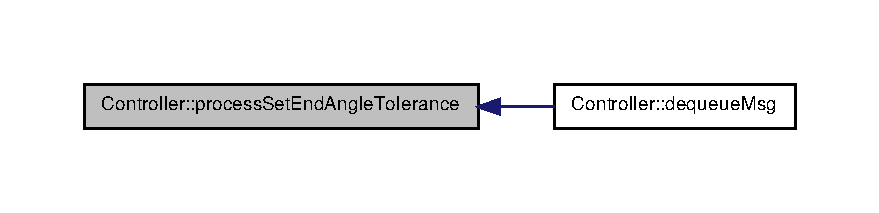
\includegraphics[width=400pt]{class_controller_a698966c052faebede44e65a0b2b16493_icgraph}
\end{center}
\end{figure}


\hypertarget{class_controller_a5a8fc3403231a34be7f4a6426c6c1954}{
\index{Controller@{Controller}!processSetEndPointTolerance@{processSetEndPointTolerance}}
\index{processSetEndPointTolerance@{processSetEndPointTolerance}!Controller@{Controller}}
\subsubsection[{processSetEndPointTolerance}]{\setlength{\rightskip}{0pt plus 5cm}virtual int Controller::processSetEndPointTolerance (
\begin{DoxyParamCaption}
\item[{{\bf SetEndPointToleranceMsg} $\ast$}]{setEndPointToleranceMsg}
\end{DoxyParamCaption}
)\hspace{0.3cm}{\ttfamily  \mbox{[}pure virtual\mbox{]}}}}
\label{class_controller_a5a8fc3403231a34be7f4a6426c6c1954}


Implemented in \hyperlink{class_my_controller_a773f4df4ced863d73b114badf007555d}{MyController}.



Here is the caller graph for this function:\nopagebreak
\begin{figure}[H]
\begin{center}
\leavevmode
\includegraphics[width=400pt]{class_controller_a5a8fc3403231a34be7f4a6426c6c1954_icgraph}
\end{center}
\end{figure}


\hypertarget{class_controller_a1a3cf77b97ccce4a364f556118ea3eb0}{
\index{Controller@{Controller}!processSetIntermediatePointTolerance@{processSetIntermediatePointTolerance}}
\index{processSetIntermediatePointTolerance@{processSetIntermediatePointTolerance}!Controller@{Controller}}
\subsubsection[{processSetIntermediatePointTolerance}]{\setlength{\rightskip}{0pt plus 5cm}virtual int Controller::processSetIntermediatePointTolerance (
\begin{DoxyParamCaption}
\item[{{\bf SetIntermediatePointToleranceMsg} $\ast$}]{setIntermediatePointToleranceMsg}
\end{DoxyParamCaption}
)\hspace{0.3cm}{\ttfamily  \mbox{[}pure virtual\mbox{]}}}}
\label{class_controller_a1a3cf77b97ccce4a364f556118ea3eb0}


Implemented in \hyperlink{class_my_controller_afe4607ed0e9fda884848671c3c3e79f4}{MyController}.



Here is the caller graph for this function:\nopagebreak
\begin{figure}[H]
\begin{center}
\leavevmode
\includegraphics[width=400pt]{class_controller_a1a3cf77b97ccce4a364f556118ea3eb0_icgraph}
\end{center}
\end{figure}


\hypertarget{class_controller_a2158164839e7019556d4785528fc5874}{
\index{Controller@{Controller}!processSetLengthUnits@{processSetLengthUnits}}
\index{processSetLengthUnits@{processSetLengthUnits}!Controller@{Controller}}
\subsubsection[{processSetLengthUnits}]{\setlength{\rightskip}{0pt plus 5cm}virtual int Controller::processSetLengthUnits (
\begin{DoxyParamCaption}
\item[{{\bf SetLengthUnitsMsg} $\ast$}]{setLengthUnitsMsg}
\end{DoxyParamCaption}
)\hspace{0.3cm}{\ttfamily  \mbox{[}pure virtual\mbox{]}}}}
\label{class_controller_a2158164839e7019556d4785528fc5874}


Implemented in \hyperlink{class_my_controller_a336fdb6e3a80e2c3d14e4ac2e7592649}{MyController}.



Here is the caller graph for this function:\nopagebreak
\begin{figure}[H]
\begin{center}
\leavevmode
\includegraphics[width=390pt]{class_controller_a2158164839e7019556d4785528fc5874_icgraph}
\end{center}
\end{figure}


\hypertarget{class_controller_a977a24df59729a6f795ea179af3d05a4}{
\index{Controller@{Controller}!processSetRelativeAcceleration@{processSetRelativeAcceleration}}
\index{processSetRelativeAcceleration@{processSetRelativeAcceleration}!Controller@{Controller}}
\subsubsection[{processSetRelativeAcceleration}]{\setlength{\rightskip}{0pt plus 5cm}virtual int Controller::processSetRelativeAcceleration (
\begin{DoxyParamCaption}
\item[{{\bf SetRelativeAccelerationMsg} $\ast$}]{setRelativeAccelerationMsg}
\end{DoxyParamCaption}
)\hspace{0.3cm}{\ttfamily  \mbox{[}pure virtual\mbox{]}}}}
\label{class_controller_a977a24df59729a6f795ea179af3d05a4}


Implemented in \hyperlink{class_my_controller_a17019de4f9ebc4d07c05d141544e4fba}{MyController}.



Here is the caller graph for this function:\nopagebreak
\begin{figure}[H]
\begin{center}
\leavevmode
\includegraphics[width=400pt]{class_controller_a977a24df59729a6f795ea179af3d05a4_icgraph}
\end{center}
\end{figure}


\hypertarget{class_controller_a25229410c00d8baf4fa2fde5fa7549c0}{
\index{Controller@{Controller}!processSetRelativeSpeed@{processSetRelativeSpeed}}
\index{processSetRelativeSpeed@{processSetRelativeSpeed}!Controller@{Controller}}
\subsubsection[{processSetRelativeSpeed}]{\setlength{\rightskip}{0pt plus 5cm}virtual int Controller::processSetRelativeSpeed (
\begin{DoxyParamCaption}
\item[{{\bf SetRelativeSpeedMsg} $\ast$}]{setRelativeSpeedMsg}
\end{DoxyParamCaption}
)\hspace{0.3cm}{\ttfamily  \mbox{[}pure virtual\mbox{]}}}}
\label{class_controller_a25229410c00d8baf4fa2fde5fa7549c0}


Implemented in \hyperlink{class_my_controller_ac073c56d47842da82036a49777e6fb64}{MyController}.



Here is the caller graph for this function:\nopagebreak
\begin{figure}[H]
\begin{center}
\leavevmode
\includegraphics[width=400pt]{class_controller_a25229410c00d8baf4fa2fde5fa7549c0_icgraph}
\end{center}
\end{figure}


\hypertarget{class_controller_a6b15d05b97d71db389603e91f0b344d0}{
\index{Controller@{Controller}!queueCloseGripper@{queueCloseGripper}}
\index{queueCloseGripper@{queueCloseGripper}!Controller@{Controller}}
\subsubsection[{queueCloseGripper}]{\setlength{\rightskip}{0pt plus 5cm}int Controller::queueCloseGripper (
\begin{DoxyParamCaption}
\item[{{\bf CloseGripperMsg}}]{closeGripperMsg}
\end{DoxyParamCaption}
)}}
\label{class_controller_a6b15d05b97d71db389603e91f0b344d0}
\hypertarget{class_controller_ad8bf10b2328e182033cd04ac6e0d8c9a}{
\index{Controller@{Controller}!queueDwell@{queueDwell}}
\index{queueDwell@{queueDwell}!Controller@{Controller}}
\subsubsection[{queueDwell}]{\setlength{\rightskip}{0pt plus 5cm}int Controller::queueDwell (
\begin{DoxyParamCaption}
\item[{{\bf DwellMsg}}]{dwellMsg}
\end{DoxyParamCaption}
)}}
\label{class_controller_ad8bf10b2328e182033cd04ac6e0d8c9a}
\hypertarget{class_controller_a45d996d1abb23d8e84edb35d04c5870f}{
\index{Controller@{Controller}!queueMsg@{queueMsg}}
\index{queueMsg@{queueMsg}!Controller@{Controller}}
\subsubsection[{queueMsg}]{\setlength{\rightskip}{0pt plus 5cm}int Controller::queueMsg (
\begin{DoxyParamCaption}
\item[{{\bf CanonicalMsg} $\ast$}]{msgIn}
\end{DoxyParamCaption}
)}}
\label{class_controller_a45d996d1abb23d8e84edb35d04c5870f}


Here is the call graph for this function:\nopagebreak
\begin{figure}[H]
\begin{center}
\leavevmode
\includegraphics[width=400pt]{class_controller_a45d996d1abb23d8e84edb35d04c5870f_cgraph}
\end{center}
\end{figure}




The documentation for this class was generated from the following files:\begin{DoxyCompactItemize}
\item 
/home/zeid/workspace/executor/src/controller/\hyperlink{controller_8hh}{controller.hh}\item 
/home/zeid/workspace/executor/src/controller/\hyperlink{controller_8cpp}{controller.cpp}\end{DoxyCompactItemize}

\hypertarget{class_d_a_o}{
\section{DAO Class Reference}
\label{class_d_a_o}\index{DAO@{DAO}}
}


{\ttfamily \#include $<$DAO.h$>$}



Collaboration diagram for DAO:\nopagebreak
\begin{figure}[H]
\begin{center}
\leavevmode
\includegraphics[width=158pt]{class_d_a_o__coll__graph}
\end{center}
\end{figure}
\subsection*{Public Member Functions}
\begin{DoxyCompactItemize}
\item 
\hyperlink{class_d_a_o_a7c20bf55e2155e4975fc0850bf8f7725}{DAO} (std::string name)
\item 
std::vector$<$ std::string $>$ \hyperlink{class_d_a_o_a079867bed71770db87a96e3b49c7ad7d}{getclassName} ()
\item 
void \hyperlink{class_d_a_o_aeec66addadd8b0010150524c3b95cfaf}{setclassName} (std::vector$<$ std::string $>$ \_\-className)
\item 
\hyperlink{class_connection}{Connection} $\ast$ \hyperlink{class_d_a_o_a5155aafd11244581b6e16597f41d0017}{getconnection} ()
\item 
void \hyperlink{class_d_a_o_afd94da4abce1ab2380d927da082bf27d}{setconnection} (\hyperlink{class_connection}{Connection} $\ast$\_\-connection)
\item 
std::map$<$ std::string, std::string $>$ \hyperlink{class_d_a_o_afa5faef8daa6b6216ab26ef8b9897db2}{get} (std::string name)
\item 
void \hyperlink{class_d_a_o_ab47618d63ada8199f67339e57e9319e7}{set} (std::map$<$ std::string, std::string $>$ data)
\end{DoxyCompactItemize}


\subsection{Constructor \& Destructor Documentation}
\hypertarget{class_d_a_o_a7c20bf55e2155e4975fc0850bf8f7725}{
\index{DAO@{DAO}!DAO@{DAO}}
\index{DAO@{DAO}!DAO@{DAO}}
\subsubsection[{DAO}]{\setlength{\rightskip}{0pt plus 5cm}DAO::DAO (
\begin{DoxyParamCaption}
\item[{std::string}]{name}
\end{DoxyParamCaption}
)}}
\label{class_d_a_o_a7c20bf55e2155e4975fc0850bf8f7725}


\subsection{Member Function Documentation}
\hypertarget{class_d_a_o_afa5faef8daa6b6216ab26ef8b9897db2}{
\index{DAO@{DAO}!get@{get}}
\index{get@{get}!DAO@{DAO}}
\subsubsection[{get}]{\setlength{\rightskip}{0pt plus 5cm}std::map$<$ std::string, std::string $>$ DAO::get (
\begin{DoxyParamCaption}
\item[{std::string}]{name}
\end{DoxyParamCaption}
)}}
\label{class_d_a_o_afa5faef8daa6b6216ab26ef8b9897db2}


Here is the call graph for this function:\nopagebreak
\begin{figure}[H]
\begin{center}
\leavevmode
\includegraphics[width=268pt]{class_d_a_o_afa5faef8daa6b6216ab26ef8b9897db2_cgraph}
\end{center}
\end{figure}




Here is the caller graph for this function:\nopagebreak
\begin{figure}[H]
\begin{center}
\leavevmode
\includegraphics[height=600pt]{class_d_a_o_afa5faef8daa6b6216ab26ef8b9897db2_icgraph}
\end{center}
\end{figure}


\hypertarget{class_d_a_o_a079867bed71770db87a96e3b49c7ad7d}{
\index{DAO@{DAO}!getclassName@{getclassName}}
\index{getclassName@{getclassName}!DAO@{DAO}}
\subsubsection[{getclassName}]{\setlength{\rightskip}{0pt plus 5cm}std::vector$<$ std::string $>$ DAO::getclassName (
\begin{DoxyParamCaption}
{}
\end{DoxyParamCaption}
)}}
\label{class_d_a_o_a079867bed71770db87a96e3b49c7ad7d}
\hypertarget{class_d_a_o_a5155aafd11244581b6e16597f41d0017}{
\index{DAO@{DAO}!getconnection@{getconnection}}
\index{getconnection@{getconnection}!DAO@{DAO}}
\subsubsection[{getconnection}]{\setlength{\rightskip}{0pt plus 5cm}{\bf Connection} $\ast$ DAO::getconnection (
\begin{DoxyParamCaption}
{}
\end{DoxyParamCaption}
)}}
\label{class_d_a_o_a5155aafd11244581b6e16597f41d0017}
\hypertarget{class_d_a_o_ab47618d63ada8199f67339e57e9319e7}{
\index{DAO@{DAO}!set@{set}}
\index{set@{set}!DAO@{DAO}}
\subsubsection[{set}]{\setlength{\rightskip}{0pt plus 5cm}void DAO::set (
\begin{DoxyParamCaption}
\item[{std::map$<$ std::string, std::string $>$}]{data}
\end{DoxyParamCaption}
)}}
\label{class_d_a_o_ab47618d63ada8199f67339e57e9319e7}


Here is the caller graph for this function:\nopagebreak
\begin{figure}[H]
\begin{center}
\leavevmode
\includegraphics[height=600pt]{class_d_a_o_ab47618d63ada8199f67339e57e9319e7_icgraph}
\end{center}
\end{figure}


\hypertarget{class_d_a_o_aeec66addadd8b0010150524c3b95cfaf}{
\index{DAO@{DAO}!setclassName@{setclassName}}
\index{setclassName@{setclassName}!DAO@{DAO}}
\subsubsection[{setclassName}]{\setlength{\rightskip}{0pt plus 5cm}void DAO::setclassName (
\begin{DoxyParamCaption}
\item[{std::vector$<$ std::string $>$}]{\_\-className}
\end{DoxyParamCaption}
)}}
\label{class_d_a_o_aeec66addadd8b0010150524c3b95cfaf}
\hypertarget{class_d_a_o_afd94da4abce1ab2380d927da082bf27d}{
\index{DAO@{DAO}!setconnection@{setconnection}}
\index{setconnection@{setconnection}!DAO@{DAO}}
\subsubsection[{setconnection}]{\setlength{\rightskip}{0pt plus 5cm}void DAO::setconnection (
\begin{DoxyParamCaption}
\item[{{\bf Connection} $\ast$}]{\_\-connection}
\end{DoxyParamCaption}
)}}
\label{class_d_a_o_afd94da4abce1ab2380d927da082bf27d}


The documentation for this class was generated from the following files:\begin{DoxyCompactItemize}
\item 
/home/zeid/workspace/executor/src/database/\hyperlink{_d_a_o_8h}{DAO.h}\item 
/home/zeid/workspace/executor/src/database/\hyperlink{_d_a_o_8cpp}{DAO.cpp}\end{DoxyCompactItemize}

\hypertarget{class_data_thing}{
\section{DataThing Class Reference}
\label{class_data_thing}\index{DataThing@{DataThing}}
}


{\ttfamily \#include $<$DataThing.h$>$}



Inheritance diagram for DataThing:\nopagebreak
\begin{figure}[H]
\begin{center}
\leavevmode
\includegraphics[width=400pt]{class_data_thing__inherit__graph}
\end{center}
\end{figure}


Collaboration diagram for DataThing:\nopagebreak
\begin{figure}[H]
\begin{center}
\leavevmode
\includegraphics[width=158pt]{class_data_thing__coll__graph}
\end{center}
\end{figure}
\subsection*{Public Member Functions}
\begin{DoxyCompactItemize}
\item 
\hyperlink{class_data_thing_a0f24c5c1cf6892915fd4e3693dac1527}{DataThing} (std::string name)
\item 
\hyperlink{class_data_thing_aab4d5d9564759368729fc7f0261e7036}{$\sim$DataThing} ()
\item 
void \hyperlink{class_data_thing_a8d294fdb8263e02e911e429aa79e8ec0}{get} (int id)
\item 
void \hyperlink{class_data_thing_ac2eac975c5f135baa984906b073920e8}{get} (std::string name)
\item 
void \hyperlink{class_data_thing_a241184e8e43c0c2e5ced27ebc0858f0f}{set} (int id, \hyperlink{class_data_thing}{DataThing} $\ast$obj)
\item 
void \hyperlink{class_data_thing_a2e3a079dcb519fa810f2d6412ba90cd3}{set} (std::string name)
\item 
std::string \hyperlink{class_data_thing_af283145e771ef8a47c853ceed4a9f963}{getname} ()
\item 
int \hyperlink{class_data_thing_a8b3d94cd97dda258c626e5851fa0cbe0}{getDataThingID} ()
\item 
\hyperlink{class_d_a_o}{DAO} $\ast$ \hyperlink{class_data_thing_ae405347375d1a67fc132f200e74637d3}{getdao} ()
\item 
void \hyperlink{class_data_thing_af13c3ba6fa5e679aaa245e22b8d16e13}{setdao} (\hyperlink{class_d_a_o}{DAO} $\ast$\_\-dao)
\item 
void \hyperlink{class_data_thing_a6d3f72340c760ce2d464fdca61a85633}{copy} (std::map$<$ std::string, std::string $>$ object)
\item 
std::vector$<$ std::string $>$ \hyperlink{class_data_thing_ad0bf28e66a55089ee19dd2a92b71244f}{Explode} (const std::string \&str, char separator)
\end{DoxyCompactItemize}


\subsection{Constructor \& Destructor Documentation}
\hypertarget{class_data_thing_a0f24c5c1cf6892915fd4e3693dac1527}{
\index{DataThing@{DataThing}!DataThing@{DataThing}}
\index{DataThing@{DataThing}!DataThing@{DataThing}}
\subsubsection[{DataThing}]{\setlength{\rightskip}{0pt plus 5cm}DataThing::DataThing (
\begin{DoxyParamCaption}
\item[{std::string}]{name}
\end{DoxyParamCaption}
)}}
\label{class_data_thing_a0f24c5c1cf6892915fd4e3693dac1527}
\hypertarget{class_data_thing_aab4d5d9564759368729fc7f0261e7036}{
\index{DataThing@{DataThing}!$\sim$DataThing@{$\sim$DataThing}}
\index{$\sim$DataThing@{$\sim$DataThing}!DataThing@{DataThing}}
\subsubsection[{$\sim$DataThing}]{\setlength{\rightskip}{0pt plus 5cm}DataThing::$\sim$DataThing (
\begin{DoxyParamCaption}
{}
\end{DoxyParamCaption}
)}}
\label{class_data_thing_aab4d5d9564759368729fc7f0261e7036}


\subsection{Member Function Documentation}
\hypertarget{class_data_thing_a6d3f72340c760ce2d464fdca61a85633}{
\index{DataThing@{DataThing}!copy@{copy}}
\index{copy@{copy}!DataThing@{DataThing}}
\subsubsection[{copy}]{\setlength{\rightskip}{0pt plus 5cm}void DataThing::copy (
\begin{DoxyParamCaption}
\item[{std::map$<$ std::string, std::string $>$}]{object}
\end{DoxyParamCaption}
)}}
\label{class_data_thing_a6d3f72340c760ce2d464fdca61a85633}


Reimplemented in \hyperlink{class_box_volume_a409bebf982f9e26fc5d4256b418589b2}{BoxVolume}, \hyperlink{class_kit_design_ac1e7f0c866efdf798bfaf965a8b551c1}{KitDesign}, \hyperlink{class_part_ref_and_pose_a0c5024f54e66320cb7b508326a192546}{PartRefAndPose}, \hyperlink{class_physical_location_a99642e6f09015649f20b98b111bb7daa}{PhysicalLocation}, \hyperlink{class_point_a46b2c683edf3223af06704fbc5da12b8}{Point}, \hyperlink{class_pose_location_a112b81b15a607f7dbe7102971caaa34f}{PoseLocation}, \hyperlink{class_pose_location_in_a6e22c098d49dd63a910681d7faa1e760}{PoseLocationIn}, \hyperlink{class_pose_location_on_a48014388aa8ab0cf554c5b119ed6cd64}{PoseLocationOn}, \hyperlink{class_pose_only_location_a6c9a967c1e1cb3b7402bbb9a4f9ee215}{PoseOnlyLocation}, \hyperlink{class_relative_location_a6d65314256e2d61ce505454dfd923b61}{RelativeLocation}, \hyperlink{class_relative_location_in_aea9c6c62540f8dbc4d93accd2904524d}{RelativeLocationIn}, \hyperlink{class_relative_location_on_ae028099fa70ceb40c4851e3852f94e81}{RelativeLocationOn}, \hyperlink{class_shape_design_a9da3d7320739c6798719f1bfe56b158d}{ShapeDesign}, \hyperlink{class_stock_keeping_unit_aa74663e5a79b178d3f0243e8e433ebd7}{StockKeepingUnit}, and \hyperlink{class_vector_ac052b5dd3cd960245f52733d724916f6}{Vector}.



Here is the caller graph for this function:\nopagebreak
\begin{figure}[H]
\begin{center}
\leavevmode
\includegraphics[width=278pt]{class_data_thing_a6d3f72340c760ce2d464fdca61a85633_icgraph}
\end{center}
\end{figure}


\hypertarget{class_data_thing_ad0bf28e66a55089ee19dd2a92b71244f}{
\index{DataThing@{DataThing}!Explode@{Explode}}
\index{Explode@{Explode}!DataThing@{DataThing}}
\subsubsection[{Explode}]{\setlength{\rightskip}{0pt plus 5cm}std::vector$<$ std::string $>$ DataThing::Explode (
\begin{DoxyParamCaption}
\item[{const std::string \&}]{str, }
\item[{char}]{separator}
\end{DoxyParamCaption}
)}}
\label{class_data_thing_ad0bf28e66a55089ee19dd2a92b71244f}


Reimplemented in \hyperlink{class_box_volume_ab463d1b1327dae19a7da471a97b3f242}{BoxVolume}, \hyperlink{class_kit_design_a613c5441521365f25d24f058e835f035}{KitDesign}, \hyperlink{class_part_ref_and_pose_a86e17ee7dd3025e5c4c223177a6dd512}{PartRefAndPose}, \hyperlink{class_physical_location_a2ab3b8277f69fe061c819039c2349f38}{PhysicalLocation}, \hyperlink{class_point_a1ddaf9ed9023f8aff7ea10e1c7ef5fe9}{Point}, \hyperlink{class_pose_location_a573ee6b74464a909cfab93cda10b7c9d}{PoseLocation}, \hyperlink{class_pose_location_in_ac6ee532cb7e7ef8be4efdb83f4454dff}{PoseLocationIn}, \hyperlink{class_pose_location_on_ab1be6bd172124568f01f1275e8b3715e}{PoseLocationOn}, \hyperlink{class_pose_only_location_abc85e3e3f6bb4acbec59b8eefd50f8f8}{PoseOnlyLocation}, \hyperlink{class_relative_location_a4993310ecce155ea78de75b56f65ac79}{RelativeLocation}, \hyperlink{class_relative_location_in_abe2fce096ef163a2d6560475eb7850fb}{RelativeLocationIn}, \hyperlink{class_relative_location_on_ae6197ea68b2c7f35cc44edfba8c0d087}{RelativeLocationOn}, \hyperlink{class_shape_design_a490d6ba1e2e22dbe6f88da126ab54a49}{ShapeDesign}, \hyperlink{class_stock_keeping_unit_a402f5d392731853e069bc0526fddd5b9}{StockKeepingUnit}, and \hyperlink{class_vector_a4be54f9589fd877120fbf0c9b799eb44}{Vector}.

\hypertarget{class_data_thing_ac2eac975c5f135baa984906b073920e8}{
\index{DataThing@{DataThing}!get@{get}}
\index{get@{get}!DataThing@{DataThing}}
\subsubsection[{get}]{\setlength{\rightskip}{0pt plus 5cm}void DataThing::get (
\begin{DoxyParamCaption}
\item[{std::string}]{name}
\end{DoxyParamCaption}
)}}
\label{class_data_thing_ac2eac975c5f135baa984906b073920e8}


Reimplemented in \hyperlink{class_box_volume_a332f433a35f192739f3570d4c8941b6a}{BoxVolume}, \hyperlink{class_kit_design_ac546195ec86a56f3581804b77128014a}{KitDesign}, \hyperlink{class_part_ref_and_pose_a420e6c89bc4fcbea3ac24c83c377a67f}{PartRefAndPose}, \hyperlink{class_physical_location_a9bfbbba56c605144b47b4e2655314681}{PhysicalLocation}, \hyperlink{class_point_a2429613b245de5c3eb064b7e33850495}{Point}, \hyperlink{class_pose_location_ac80d95846f773d86e3d6cfc97bed779c}{PoseLocation}, \hyperlink{class_pose_location_in_a91d60b119ddf6254472751d0346cba9c}{PoseLocationIn}, \hyperlink{class_pose_location_on_a492a9e2663a3613a8d408a73bd5e1db2}{PoseLocationOn}, \hyperlink{class_pose_only_location_a6cf43cbfcfa2673e114007d7f0b76f21}{PoseOnlyLocation}, \hyperlink{class_relative_location_a5a3ae66baa899f3b26e906087a880955}{RelativeLocation}, \hyperlink{class_relative_location_in_a9fceea9cfff69f10c2d4f232b6cdf978}{RelativeLocationIn}, \hyperlink{class_relative_location_on_a6d883f6f937538e2f27a24c2ba12f9c0}{RelativeLocationOn}, \hyperlink{class_shape_design_ae2e1f8b4b42df5ca45ac96f4ec62daa8}{ShapeDesign}, \hyperlink{class_stock_keeping_unit_a28cc44a2000d0c834e03456f96543bff}{StockKeepingUnit}, and \hyperlink{class_vector_a7ee6ab6d31fbcdb8bd48dd030e30a1af}{Vector}.



Here is the call graph for this function:\nopagebreak
\begin{figure}[H]
\begin{center}
\leavevmode
\includegraphics[width=400pt]{class_data_thing_ac2eac975c5f135baa984906b073920e8_cgraph}
\end{center}
\end{figure}


\hypertarget{class_data_thing_a8d294fdb8263e02e911e429aa79e8ec0}{
\index{DataThing@{DataThing}!get@{get}}
\index{get@{get}!DataThing@{DataThing}}
\subsubsection[{get}]{\setlength{\rightskip}{0pt plus 5cm}void DataThing::get (
\begin{DoxyParamCaption}
\item[{int}]{id}
\end{DoxyParamCaption}
)}}
\label{class_data_thing_a8d294fdb8263e02e911e429aa79e8ec0}


Reimplemented in \hyperlink{class_box_volume_ad5470426b7ed060920fb0cd701a0eba7}{BoxVolume}, \hyperlink{class_kit_design_a671fab4903d3eee18e7a2bd7973f344f}{KitDesign}, \hyperlink{class_part_ref_and_pose_a1bc285545c59e1debf4a21316782f9fa}{PartRefAndPose}, \hyperlink{class_physical_location_addcfd9162a1ac9b8938e4718789095c6}{PhysicalLocation}, \hyperlink{class_point_a6fea183c8c7514ff6657d1bb43b785cb}{Point}, \hyperlink{class_pose_location_a8b05ffe2202af40a22e7dcd4a7a0bec3}{PoseLocation}, \hyperlink{class_pose_location_in_a717cd5951630120110887cac063facb3}{PoseLocationIn}, \hyperlink{class_pose_location_on_a77df4e49b397b0f4396c27ac95a16734}{PoseLocationOn}, \hyperlink{class_pose_only_location_afbdc6742455d0030005d84eb29875c71}{PoseOnlyLocation}, \hyperlink{class_relative_location_aba3ac6526140bd3e9ea10b2c08362daa}{RelativeLocation}, \hyperlink{class_relative_location_in_ad3c625cef3df3f1900ae07cd35206cd1}{RelativeLocationIn}, \hyperlink{class_relative_location_on_a99ffe13fe5872cca3370f47d8deae887}{RelativeLocationOn}, \hyperlink{class_shape_design_aefc72191093f49bf73fa4a87bdf3f1b4}{ShapeDesign}, \hyperlink{class_stock_keeping_unit_a03f9d33f0a8e6f9315e853967aac158c}{StockKeepingUnit}, and \hyperlink{class_vector_ad325eaf33ebd1ca02ba082f172601a4f}{Vector}.

\hypertarget{class_data_thing_ae405347375d1a67fc132f200e74637d3}{
\index{DataThing@{DataThing}!getdao@{getdao}}
\index{getdao@{getdao}!DataThing@{DataThing}}
\subsubsection[{getdao}]{\setlength{\rightskip}{0pt plus 5cm}{\bf DAO} $\ast$ DataThing::getdao (
\begin{DoxyParamCaption}
{}
\end{DoxyParamCaption}
)}}
\label{class_data_thing_ae405347375d1a67fc132f200e74637d3}


Reimplemented in \hyperlink{class_box_volume_ab39b3c8e7c434e9a963f5c538b3ee84e}{BoxVolume}, \hyperlink{class_kit_design_af11875a1c4f876c2e328f94e38d900ce}{KitDesign}, \hyperlink{class_part_ref_and_pose_a1735464fcf7babfc87ec8d5968c48ca4}{PartRefAndPose}, \hyperlink{class_physical_location_a69e1ec1ea1add99b2de138be01622374}{PhysicalLocation}, \hyperlink{class_point_a388f755bac4026d6d24ceb3d49117707}{Point}, \hyperlink{class_pose_location_a53b620b3918557714158a297bc90b257}{PoseLocation}, \hyperlink{class_pose_location_in_a91db9c4b46c96f2a443fb08a7738faaa}{PoseLocationIn}, \hyperlink{class_pose_location_on_af2f51f0dbb23646d082f5c2237dac3a1}{PoseLocationOn}, \hyperlink{class_pose_only_location_ab701be60dda6cf1be3bb3fd6098c557c}{PoseOnlyLocation}, \hyperlink{class_relative_location_add367c3d25d6016ba594c5a5b1b0ea79}{RelativeLocation}, \hyperlink{class_relative_location_in_ab695d2876ac7cf7f56f4266380ab8cca}{RelativeLocationIn}, \hyperlink{class_relative_location_on_a7d019a99bd77570d272e4b209162382d}{RelativeLocationOn}, \hyperlink{class_shape_design_aff1853621aa7cb5a0fdc0c0061ab543a}{ShapeDesign}, \hyperlink{class_stock_keeping_unit_a118a016c0cb48facfa87eceeeaa75f68}{StockKeepingUnit}, and \hyperlink{class_vector_ab6ce67669fa54699473f2754227a224c}{Vector}.

\hypertarget{class_data_thing_a8b3d94cd97dda258c626e5851fa0cbe0}{
\index{DataThing@{DataThing}!getDataThingID@{getDataThingID}}
\index{getDataThingID@{getDataThingID}!DataThing@{DataThing}}
\subsubsection[{getDataThingID}]{\setlength{\rightskip}{0pt plus 5cm}int DataThing::getDataThingID (
\begin{DoxyParamCaption}
{}
\end{DoxyParamCaption}
)}}
\label{class_data_thing_a8b3d94cd97dda258c626e5851fa0cbe0}
\hypertarget{class_data_thing_af283145e771ef8a47c853ceed4a9f963}{
\index{DataThing@{DataThing}!getname@{getname}}
\index{getname@{getname}!DataThing@{DataThing}}
\subsubsection[{getname}]{\setlength{\rightskip}{0pt plus 5cm}std::string DataThing::getname (
\begin{DoxyParamCaption}
{}
\end{DoxyParamCaption}
)}}
\label{class_data_thing_af283145e771ef8a47c853ceed4a9f963}


Reimplemented in \hyperlink{class_box_volume_a786f06a3a9b3c1feff8aa120b449f5de}{BoxVolume}, \hyperlink{class_kit_design_a83ed6018e368cdbe15355b6a124fc221}{KitDesign}, \hyperlink{class_part_ref_and_pose_a4c0143e30e5398e014869db932d117ac}{PartRefAndPose}, \hyperlink{class_physical_location_a80fa2cb0593f5cb050e02f30d41e2fbe}{PhysicalLocation}, \hyperlink{class_point_afc547192531382caf91fadf15d9b9422}{Point}, \hyperlink{class_pose_location_aaa31295a8214a697e4daa577f687f2f4}{PoseLocation}, \hyperlink{class_pose_location_in_a22fa79ef529f695db02ff986444f976e}{PoseLocationIn}, \hyperlink{class_pose_location_on_ab2ee4698cae78d63ab67919bd2a2f17e}{PoseLocationOn}, \hyperlink{class_pose_only_location_aa0c28cd150879da0d59275678e618569}{PoseOnlyLocation}, \hyperlink{class_relative_location_a6cbb08ce7d4aedfd5d1d0ea768ede450}{RelativeLocation}, \hyperlink{class_relative_location_in_a6a3f7623911d954ee50c3231c93f2b7c}{RelativeLocationIn}, \hyperlink{class_relative_location_on_a8307b4dd51ea5a60d1f737868fd8f4a3}{RelativeLocationOn}, \hyperlink{class_shape_design_a0c1cddad8b051becd70ddc56f312615b}{ShapeDesign}, \hyperlink{class_stock_keeping_unit_aea522e6162d4639ab19ef0069f3336eb}{StockKeepingUnit}, and \hyperlink{class_vector_abf0dfbf85e6c8431b15fe58885ab33fc}{Vector}.

\hypertarget{class_data_thing_a2e3a079dcb519fa810f2d6412ba90cd3}{
\index{DataThing@{DataThing}!set@{set}}
\index{set@{set}!DataThing@{DataThing}}
\subsubsection[{set}]{\setlength{\rightskip}{0pt plus 5cm}void DataThing::set (
\begin{DoxyParamCaption}
\item[{std::string}]{name}
\end{DoxyParamCaption}
)}}
\label{class_data_thing_a2e3a079dcb519fa810f2d6412ba90cd3}


Reimplemented in \hyperlink{class_box_volume_a4aa7c183fec52b57fab6d509e5e87e5a}{BoxVolume}, \hyperlink{class_kit_design_abf2d5f0803a8002ede4a777a6fa53cbf}{KitDesign}, \hyperlink{class_part_ref_and_pose_a722227d5b2ff0c61e4bc8a74e7bd8597}{PartRefAndPose}, \hyperlink{class_physical_location_a7d41ac762e3ea3bb544225ac0a774e2e}{PhysicalLocation}, \hyperlink{class_point_a4a2013c10fb10b5c62c7b4c6fba14dfe}{Point}, \hyperlink{class_pose_location_abf15870fff773935c4ab02f01cd47eac}{PoseLocation}, \hyperlink{class_pose_location_in_a57e44bf1ccaadd0e58277d1d1feebcee}{PoseLocationIn}, \hyperlink{class_pose_location_on_a2c3e33342ab68431d3657cf8a34d9347}{PoseLocationOn}, \hyperlink{class_pose_only_location_aa9b42c8410326f74ca5f11110e6b3d76}{PoseOnlyLocation}, \hyperlink{class_relative_location_a42d75e6b768859f46d5b52c6fd9786e4}{RelativeLocation}, \hyperlink{class_relative_location_in_abe3029770e3c23c2930a880299832bb7}{RelativeLocationIn}, \hyperlink{class_relative_location_on_a3314371d4fcabe2d074d8d96f32ee7e1}{RelativeLocationOn}, \hyperlink{class_shape_design_a29cef64365065520c765ca7df0a8a485}{ShapeDesign}, \hyperlink{class_stock_keeping_unit_ad7241fe76fce2b27704a1c68e9c78edd}{StockKeepingUnit}, and \hyperlink{class_vector_a41a1d931298f149ca5433331da53a765}{Vector}.



Here is the call graph for this function:\nopagebreak
\begin{figure}[H]
\begin{center}
\leavevmode
\includegraphics[width=246pt]{class_data_thing_a2e3a079dcb519fa810f2d6412ba90cd3_cgraph}
\end{center}
\end{figure}


\hypertarget{class_data_thing_a241184e8e43c0c2e5ced27ebc0858f0f}{
\index{DataThing@{DataThing}!set@{set}}
\index{set@{set}!DataThing@{DataThing}}
\subsubsection[{set}]{\setlength{\rightskip}{0pt plus 5cm}void DataThing::set (
\begin{DoxyParamCaption}
\item[{int}]{id, }
\item[{{\bf DataThing} $\ast$}]{obj}
\end{DoxyParamCaption}
)}}
\label{class_data_thing_a241184e8e43c0c2e5ced27ebc0858f0f}
\hypertarget{class_data_thing_af13c3ba6fa5e679aaa245e22b8d16e13}{
\index{DataThing@{DataThing}!setdao@{setdao}}
\index{setdao@{setdao}!DataThing@{DataThing}}
\subsubsection[{setdao}]{\setlength{\rightskip}{0pt plus 5cm}void DataThing::setdao (
\begin{DoxyParamCaption}
\item[{{\bf DAO} $\ast$}]{\_\-dao}
\end{DoxyParamCaption}
)}}
\label{class_data_thing_af13c3ba6fa5e679aaa245e22b8d16e13}


Reimplemented in \hyperlink{class_box_volume_ad186a540505ac006ee58952ecaed35f8}{BoxVolume}, \hyperlink{class_kit_design_aea131638fcfa0e95c9152a60d62e0233}{KitDesign}, \hyperlink{class_part_ref_and_pose_a4089d24393c5b710e86d7841dde07bdd}{PartRefAndPose}, \hyperlink{class_physical_location_a22e72cd2fbf6d9b68192622961e8e4ce}{PhysicalLocation}, \hyperlink{class_point_a505b2c2e820cf9ef9dfdc66738a8c151}{Point}, \hyperlink{class_pose_location_a86c7f6e2a4610954bc530864d6d8ec52}{PoseLocation}, \hyperlink{class_pose_location_in_a0ed7e6d3b25f39f6cd6695f2675c595f}{PoseLocationIn}, \hyperlink{class_pose_location_on_a9948176529b12221d938e1e5b1828149}{PoseLocationOn}, \hyperlink{class_pose_only_location_aa51f136b549fd9ddc9a89246fa94c5bc}{PoseOnlyLocation}, \hyperlink{class_relative_location_a90865b7d18772c0fd40e71b2132f3f06}{RelativeLocation}, \hyperlink{class_relative_location_in_a62d119b3aac2aa9e728878a85971c7ce}{RelativeLocationIn}, \hyperlink{class_relative_location_on_a37515a33b782962408999037a2880654}{RelativeLocationOn}, \hyperlink{class_shape_design_a06b9ee8b31a62eca03a14adaa90626cf}{ShapeDesign}, \hyperlink{class_stock_keeping_unit_abeffab863d6d7bc4cc59d547c82f3815}{StockKeepingUnit}, and \hyperlink{class_vector_a164215fcc47e016d863562eb5ff93524}{Vector}.



The documentation for this class was generated from the following files:\begin{DoxyCompactItemize}
\item 
/home/zeid/workspace/executor/src/database/\hyperlink{_data_thing_8h}{DataThing.h}\item 
/home/zeid/workspace/executor/src/database/\hyperlink{_data_thing_8cpp}{DataThing.cpp}\end{DoxyCompactItemize}

\hypertarget{class_dwell_msg}{
\section{DwellMsg Class Reference}
\label{class_dwell_msg}\index{DwellMsg@{DwellMsg}}
}


{\ttfamily \#include $<$canonicalMsg.hh$>$}



Inheritance diagram for DwellMsg:\nopagebreak
\begin{figure}[H]
\begin{center}
\leavevmode
\includegraphics[width=156pt]{class_dwell_msg__inherit__graph}
\end{center}
\end{figure}


Collaboration diagram for DwellMsg:\nopagebreak
\begin{figure}[H]
\begin{center}
\leavevmode
\includegraphics[width=156pt]{class_dwell_msg__coll__graph}
\end{center}
\end{figure}
\subsection*{Public Member Functions}
\begin{DoxyCompactItemize}
\item 
\hyperlink{class_dwell_msg_a7d71a7c93a9db45bf87678b006fc0fdb}{DwellMsg} ()
\item 
\hyperlink{class_dwell_msg_a76dbe2536d5abf593768e59d3b1bac9b}{DwellMsg} (double timeIn)
\item 
\hyperlink{class_dwell_msg_acce14108a4cf651e4c241ba906bf6bc1}{$\sim$DwellMsg} ()
\end{DoxyCompactItemize}
\subsection*{Public Attributes}
\begin{DoxyCompactItemize}
\item 
double \hyperlink{class_dwell_msg_a33c85532f94bc20af83057d3220a94c5}{time}
\end{DoxyCompactItemize}


\subsection{Constructor \& Destructor Documentation}
\hypertarget{class_dwell_msg_a7d71a7c93a9db45bf87678b006fc0fdb}{
\index{DwellMsg@{DwellMsg}!DwellMsg@{DwellMsg}}
\index{DwellMsg@{DwellMsg}!DwellMsg@{DwellMsg}}
\subsubsection[{DwellMsg}]{\setlength{\rightskip}{0pt plus 5cm}DwellMsg::DwellMsg (
\begin{DoxyParamCaption}
{}
\end{DoxyParamCaption}
)\hspace{0.3cm}{\ttfamily  \mbox{[}inline\mbox{]}}}}
\label{class_dwell_msg_a7d71a7c93a9db45bf87678b006fc0fdb}
\hypertarget{class_dwell_msg_a76dbe2536d5abf593768e59d3b1bac9b}{
\index{DwellMsg@{DwellMsg}!DwellMsg@{DwellMsg}}
\index{DwellMsg@{DwellMsg}!DwellMsg@{DwellMsg}}
\subsubsection[{DwellMsg}]{\setlength{\rightskip}{0pt plus 5cm}DwellMsg::DwellMsg (
\begin{DoxyParamCaption}
\item[{double}]{timeIn}
\end{DoxyParamCaption}
)\hspace{0.3cm}{\ttfamily  \mbox{[}inline\mbox{]}}}}
\label{class_dwell_msg_a76dbe2536d5abf593768e59d3b1bac9b}
\hypertarget{class_dwell_msg_acce14108a4cf651e4c241ba906bf6bc1}{
\index{DwellMsg@{DwellMsg}!$\sim$DwellMsg@{$\sim$DwellMsg}}
\index{$\sim$DwellMsg@{$\sim$DwellMsg}!DwellMsg@{DwellMsg}}
\subsubsection[{$\sim$DwellMsg}]{\setlength{\rightskip}{0pt plus 5cm}DwellMsg::$\sim$DwellMsg (
\begin{DoxyParamCaption}
{}
\end{DoxyParamCaption}
)\hspace{0.3cm}{\ttfamily  \mbox{[}inline\mbox{]}}}}
\label{class_dwell_msg_acce14108a4cf651e4c241ba906bf6bc1}


\subsection{Member Data Documentation}
\hypertarget{class_dwell_msg_a33c85532f94bc20af83057d3220a94c5}{
\index{DwellMsg@{DwellMsg}!time@{time}}
\index{time@{time}!DwellMsg@{DwellMsg}}
\subsubsection[{time}]{\setlength{\rightskip}{0pt plus 5cm}double {\bf DwellMsg::time}}}
\label{class_dwell_msg_a33c85532f94bc20af83057d3220a94c5}


The documentation for this class was generated from the following file:\begin{DoxyCompactItemize}
\item 
/home/zeid/workspace/executor/src/controller/\hyperlink{canonical_msg_8hh}{canonicalMsg.hh}\end{DoxyCompactItemize}

\hypertarget{class_end_canon_msg}{
\section{EndCanonMsg Class Reference}
\label{class_end_canon_msg}\index{EndCanonMsg@{EndCanonMsg}}
}


{\ttfamily \#include $<$canonicalMsg.hh$>$}



Inheritance diagram for EndCanonMsg:\nopagebreak
\begin{figure}[H]
\begin{center}
\leavevmode
\includegraphics[width=158pt]{class_end_canon_msg__inherit__graph}
\end{center}
\end{figure}


Collaboration diagram for EndCanonMsg:\nopagebreak
\begin{figure}[H]
\begin{center}
\leavevmode
\includegraphics[width=158pt]{class_end_canon_msg__coll__graph}
\end{center}
\end{figure}
\subsection*{Public Member Functions}
\begin{DoxyCompactItemize}
\item 
\hyperlink{class_end_canon_msg_a8581204a18959908e6034f7b61c1b0f5}{EndCanonMsg} ()
\item 
\hyperlink{class_end_canon_msg_a7dda78bafe176888f5926ac7562e4eb7}{EndCanonMsg} (int reasonIn)
\item 
\hyperlink{class_end_canon_msg_a7d916d2072591c4d2f24410a69d8746e}{$\sim$EndCanonMsg} ()
\end{DoxyCompactItemize}
\subsection*{Public Attributes}
\begin{DoxyCompactItemize}
\item 
int \hyperlink{class_end_canon_msg_a80f182724d15f5994b0231bd40dee9e7}{reason}
\end{DoxyCompactItemize}


\subsection{Constructor \& Destructor Documentation}
\hypertarget{class_end_canon_msg_a8581204a18959908e6034f7b61c1b0f5}{
\index{EndCanonMsg@{EndCanonMsg}!EndCanonMsg@{EndCanonMsg}}
\index{EndCanonMsg@{EndCanonMsg}!EndCanonMsg@{EndCanonMsg}}
\subsubsection[{EndCanonMsg}]{\setlength{\rightskip}{0pt plus 5cm}EndCanonMsg::EndCanonMsg (
\begin{DoxyParamCaption}
{}
\end{DoxyParamCaption}
)\hspace{0.3cm}{\ttfamily  \mbox{[}inline\mbox{]}}}}
\label{class_end_canon_msg_a8581204a18959908e6034f7b61c1b0f5}
\hypertarget{class_end_canon_msg_a7dda78bafe176888f5926ac7562e4eb7}{
\index{EndCanonMsg@{EndCanonMsg}!EndCanonMsg@{EndCanonMsg}}
\index{EndCanonMsg@{EndCanonMsg}!EndCanonMsg@{EndCanonMsg}}
\subsubsection[{EndCanonMsg}]{\setlength{\rightskip}{0pt plus 5cm}EndCanonMsg::EndCanonMsg (
\begin{DoxyParamCaption}
\item[{int}]{reasonIn}
\end{DoxyParamCaption}
)\hspace{0.3cm}{\ttfamily  \mbox{[}inline\mbox{]}}}}
\label{class_end_canon_msg_a7dda78bafe176888f5926ac7562e4eb7}
\hypertarget{class_end_canon_msg_a7d916d2072591c4d2f24410a69d8746e}{
\index{EndCanonMsg@{EndCanonMsg}!$\sim$EndCanonMsg@{$\sim$EndCanonMsg}}
\index{$\sim$EndCanonMsg@{$\sim$EndCanonMsg}!EndCanonMsg@{EndCanonMsg}}
\subsubsection[{$\sim$EndCanonMsg}]{\setlength{\rightskip}{0pt plus 5cm}EndCanonMsg::$\sim$EndCanonMsg (
\begin{DoxyParamCaption}
{}
\end{DoxyParamCaption}
)\hspace{0.3cm}{\ttfamily  \mbox{[}inline\mbox{]}}}}
\label{class_end_canon_msg_a7d916d2072591c4d2f24410a69d8746e}


\subsection{Member Data Documentation}
\hypertarget{class_end_canon_msg_a80f182724d15f5994b0231bd40dee9e7}{
\index{EndCanonMsg@{EndCanonMsg}!reason@{reason}}
\index{reason@{reason}!EndCanonMsg@{EndCanonMsg}}
\subsubsection[{reason}]{\setlength{\rightskip}{0pt plus 5cm}int {\bf EndCanonMsg::reason}}}
\label{class_end_canon_msg_a80f182724d15f5994b0231bd40dee9e7}


The documentation for this class was generated from the following file:\begin{DoxyCompactItemize}
\item 
/home/zeid/workspace/executor/src/controller/\hyperlink{canonical_msg_8hh}{canonicalMsg.hh}\end{DoxyCompactItemize}

\hypertarget{class_end_effector}{
\section{EndEffector Class Reference}
\label{class_end_effector}\index{EndEffector@{EndEffector}}
}


{\ttfamily \#include $<$EndEffector.h$>$}



Inheritance diagram for EndEffector:\nopagebreak
\begin{figure}[H]
\begin{center}
\leavevmode
\includegraphics[width=347pt]{class_end_effector__inherit__graph}
\end{center}
\end{figure}


Collaboration diagram for EndEffector:\nopagebreak
\begin{figure}[H]
\begin{center}
\leavevmode
\includegraphics[width=400pt]{class_end_effector__coll__graph}
\end{center}
\end{figure}
\subsection*{Public Member Functions}
\begin{DoxyCompactItemize}
\item 
\hyperlink{class_end_effector_a97a5bb4d8630ff0ba0fc172b6dc01f15}{EndEffector} (std::string name)
\item 
\hyperlink{class_end_effector_a0ffb936e23ecc47b7b52088c558be7b9}{$\sim$EndEffector} ()
\item 
void \hyperlink{class_end_effector_a7edd1d305e1316dffda82a9d66a9564b}{get} (int id)
\item 
void \hyperlink{class_end_effector_ad46cf6320eb6ee331316a14b1095e8d8}{get} (std::string name)
\item 
void \hyperlink{class_end_effector_af6f2d56c3724fc82bcd6e8143fee05f2}{set} (int id, \hyperlink{class_end_effector}{EndEffector} $\ast$obj)
\item 
void \hyperlink{class_end_effector_a6361b8a7cb17a441de501387a1006993}{set} (std::string name)
\item 
std::string \hyperlink{class_end_effector_ae60df01deb3d460cec2832cd7617bddf}{gethasEndEffector\_\-Description} ()
\item 
void \hyperlink{class_end_effector_aa68b47f17d8444d0ce30cf573ab5f664}{sethasEndEffector\_\-Description} (std::string \_\-hasEndEffector\_\-Description)
\item 
double \hyperlink{class_end_effector_af494832528732f347cc1211aa7d5d677}{gethasEndEffector\_\-Weight} ()
\item 
void \hyperlink{class_end_effector_a3596de8e005b33c99d6d18e1c2e92d58}{sethasEndEffector\_\-Weight} (double \_\-hasEndEffector\_\-Weight)
\item 
double \hyperlink{class_end_effector_a158d0e1ecf0a0ef4c7f6686cedeee634}{gethasEffector\_\-MaximumLoadWeight} ()
\item 
void \hyperlink{class_end_effector_ac21ccbd72ce8bea4c1e8eed751958c4f}{sethasEffector\_\-MaximumLoadWeight} (double \_\-hasEffector\_\-MaximumLoadWeight)
\item 
std::string \hyperlink{class_end_effector_a154fcb6fee46342d7dc03b69359433d0}{gethasEndEffector\_\-Id} ()
\item 
void \hyperlink{class_end_effector_aa41a5c32cb0c03bd5f138b5e426c3834}{sethasEndEffector\_\-Id} (std::string \_\-hasEndEffector\_\-Id)
\item 
std::string \hyperlink{class_end_effector_a36e103bed34f4354487211af69eaea93}{getname} ()
\item 
int \hyperlink{class_end_effector_a89452bc420683832af0e2d55f10b6435}{getEndEffectorID} ()
\item 
\hyperlink{class_d_a_o}{DAO} $\ast$ \hyperlink{class_end_effector_ab4e27c958cdd62573d064acde55d6304}{getdao} ()
\item 
void \hyperlink{class_end_effector_a68f208f457189aa356951442d5692b08}{setdao} (\hyperlink{class_d_a_o}{DAO} $\ast$\_\-dao)
\item 
\hyperlink{class_robot}{Robot} $\ast$ \hyperlink{class_end_effector_a4eb16ef6e361e33561f4f1791296c831}{gethadByEndEffector\_\-Robot} ()
\item 
void \hyperlink{class_end_effector_a5b47bcb2d71bdd47fc669cab55dd95f1}{sethadByEndEffector\_\-Robot} (\hyperlink{class_robot}{Robot} $\ast$\_\-hadByEndEffector\_\-Robot)
\item 
\hyperlink{class_end_effector_holder}{EndEffectorHolder} $\ast$ \hyperlink{class_end_effector_a5414f06b3c972765027c55f42f7f4fa8}{gethasEndEffectorHolder\_\-EndEffector} ()
\item 
void \hyperlink{class_end_effector_a92135e5590b09cc347f921107dbde707}{sethasEndEffectorHolder\_\-EndEffector} (\hyperlink{class_end_effector_holder}{EndEffectorHolder} $\ast$\_\-hasEndEffectorHolder\_\-EndEffector)
\item 
void \hyperlink{class_end_effector_a60c32047ac0826ef80a10b8477132d7c}{copy} (std::map$<$ std::string, std::string $>$ object)
\item 
std::vector$<$ std::string $>$ \hyperlink{class_end_effector_a29555a56acdff435557ac14e5d3dcd47}{Explode} (const std::string \&str, char separator)
\end{DoxyCompactItemize}


\subsection{Constructor \& Destructor Documentation}
\hypertarget{class_end_effector_a97a5bb4d8630ff0ba0fc172b6dc01f15}{
\index{EndEffector@{EndEffector}!EndEffector@{EndEffector}}
\index{EndEffector@{EndEffector}!EndEffector@{EndEffector}}
\subsubsection[{EndEffector}]{\setlength{\rightskip}{0pt plus 5cm}EndEffector::EndEffector (
\begin{DoxyParamCaption}
\item[{std::string}]{name}
\end{DoxyParamCaption}
)}}
\label{class_end_effector_a97a5bb4d8630ff0ba0fc172b6dc01f15}
\hypertarget{class_end_effector_a0ffb936e23ecc47b7b52088c558be7b9}{
\index{EndEffector@{EndEffector}!$\sim$EndEffector@{$\sim$EndEffector}}
\index{$\sim$EndEffector@{$\sim$EndEffector}!EndEffector@{EndEffector}}
\subsubsection[{$\sim$EndEffector}]{\setlength{\rightskip}{0pt plus 5cm}EndEffector::$\sim$EndEffector (
\begin{DoxyParamCaption}
{}
\end{DoxyParamCaption}
)}}
\label{class_end_effector_a0ffb936e23ecc47b7b52088c558be7b9}


\subsection{Member Function Documentation}
\hypertarget{class_end_effector_a60c32047ac0826ef80a10b8477132d7c}{
\index{EndEffector@{EndEffector}!copy@{copy}}
\index{copy@{copy}!EndEffector@{EndEffector}}
\subsubsection[{copy}]{\setlength{\rightskip}{0pt plus 5cm}void EndEffector::copy (
\begin{DoxyParamCaption}
\item[{std::map$<$ std::string, std::string $>$}]{object}
\end{DoxyParamCaption}
)}}
\label{class_end_effector_a60c32047ac0826ef80a10b8477132d7c}


Reimplemented from \hyperlink{class_solid_object_ac3c576278aad2366890e96889d7e24cf}{SolidObject}.



Reimplemented in \hyperlink{class_gripper_effector_a446ce56a6195c2b0dcccc6a6fcdd1961}{GripperEffector}, \hyperlink{class_vacuum_effector_ac180edaaca8f4bd76cb28f21f0846e3b}{VacuumEffector}, \hyperlink{class_vacuum_effector_multi_cup_a4fc22178c8e73ce173566e34a451843c}{VacuumEffectorMultiCup}, and \hyperlink{class_vacuum_effector_single_cup_a3a4386ea65ec07e7279301c6a26579a3}{VacuumEffectorSingleCup}.



Here is the caller graph for this function:\nopagebreak
\begin{figure}[H]
\begin{center}
\leavevmode
\includegraphics[width=286pt]{class_end_effector_a60c32047ac0826ef80a10b8477132d7c_icgraph}
\end{center}
\end{figure}


\hypertarget{class_end_effector_a29555a56acdff435557ac14e5d3dcd47}{
\index{EndEffector@{EndEffector}!Explode@{Explode}}
\index{Explode@{Explode}!EndEffector@{EndEffector}}
\subsubsection[{Explode}]{\setlength{\rightskip}{0pt plus 5cm}std::vector$<$ std::string $>$ EndEffector::Explode (
\begin{DoxyParamCaption}
\item[{const std::string \&}]{str, }
\item[{char}]{separator}
\end{DoxyParamCaption}
)}}
\label{class_end_effector_a29555a56acdff435557ac14e5d3dcd47}


Reimplemented from \hyperlink{class_solid_object_a9c68e5f4e7a8bf41ab5d99736063f07c}{SolidObject}.



Reimplemented in \hyperlink{class_gripper_effector_a93cffef39860f2c94a09e52531cfabc2}{GripperEffector}, \hyperlink{class_vacuum_effector_adc7ad7b080152922047eba5b51834c05}{VacuumEffector}, \hyperlink{class_vacuum_effector_multi_cup_acb7d89807c0207aaa7399b16667cb1a4}{VacuumEffectorMultiCup}, and \hyperlink{class_vacuum_effector_single_cup_aca38516cf8a90a4ad1bad726f2d82386}{VacuumEffectorSingleCup}.

\hypertarget{class_end_effector_a7edd1d305e1316dffda82a9d66a9564b}{
\index{EndEffector@{EndEffector}!get@{get}}
\index{get@{get}!EndEffector@{EndEffector}}
\subsubsection[{get}]{\setlength{\rightskip}{0pt plus 5cm}void EndEffector::get (
\begin{DoxyParamCaption}
\item[{int}]{id}
\end{DoxyParamCaption}
)}}
\label{class_end_effector_a7edd1d305e1316dffda82a9d66a9564b}


Reimplemented from \hyperlink{class_solid_object_a76502cdc5f302d769508f196a0358d04}{SolidObject}.



Reimplemented in \hyperlink{class_gripper_effector_a0e8f17336a915c587ce5338db0cee9bc}{GripperEffector}, \hyperlink{class_vacuum_effector_ad61efa5e78bbcd8295b09c78488f013e}{VacuumEffector}, \hyperlink{class_vacuum_effector_multi_cup_a9572b300d529c6615a1e954d78d2242b}{VacuumEffectorMultiCup}, and \hyperlink{class_vacuum_effector_single_cup_a9f70755bcbc4befc7ec7d4bf4bed77d2}{VacuumEffectorSingleCup}.

\hypertarget{class_end_effector_ad46cf6320eb6ee331316a14b1095e8d8}{
\index{EndEffector@{EndEffector}!get@{get}}
\index{get@{get}!EndEffector@{EndEffector}}
\subsubsection[{get}]{\setlength{\rightskip}{0pt plus 5cm}void EndEffector::get (
\begin{DoxyParamCaption}
\item[{std::string}]{name}
\end{DoxyParamCaption}
)}}
\label{class_end_effector_ad46cf6320eb6ee331316a14b1095e8d8}


Reimplemented from \hyperlink{class_solid_object_afb027c9baf0d811d6f376abc10501ac9}{SolidObject}.



Reimplemented in \hyperlink{class_gripper_effector_ade0d2f1e5e0a61d1550ffcc305eae11e}{GripperEffector}, \hyperlink{class_vacuum_effector_a7424e643d7c5440e7f988c2321b78c20}{VacuumEffector}, \hyperlink{class_vacuum_effector_multi_cup_a414494076a456ad84adf4784e1c216d7}{VacuumEffectorMultiCup}, and \hyperlink{class_vacuum_effector_single_cup_a5ae1745edb7c88858b86df5d3f74297c}{VacuumEffectorSingleCup}.



Here is the call graph for this function:\nopagebreak
\begin{figure}[H]
\begin{center}
\leavevmode
\includegraphics[width=400pt]{class_end_effector_ad46cf6320eb6ee331316a14b1095e8d8_cgraph}
\end{center}
\end{figure}


\hypertarget{class_end_effector_ab4e27c958cdd62573d064acde55d6304}{
\index{EndEffector@{EndEffector}!getdao@{getdao}}
\index{getdao@{getdao}!EndEffector@{EndEffector}}
\subsubsection[{getdao}]{\setlength{\rightskip}{0pt plus 5cm}{\bf DAO} $\ast$ EndEffector::getdao (
\begin{DoxyParamCaption}
{}
\end{DoxyParamCaption}
)}}
\label{class_end_effector_ab4e27c958cdd62573d064acde55d6304}


Reimplemented from \hyperlink{class_solid_object_a82697845082b48fb3b2b90606e68259a}{SolidObject}.



Reimplemented in \hyperlink{class_gripper_effector_a184c5ca2103576a291ee4bafe0c0d5a3}{GripperEffector}, \hyperlink{class_vacuum_effector_ae877acc2e7d9a57e10991b5b3b9478de}{VacuumEffector}, \hyperlink{class_vacuum_effector_multi_cup_a784d66a07083715cb21841c20bccb1b9}{VacuumEffectorMultiCup}, and \hyperlink{class_vacuum_effector_single_cup_ab0b1538f9de12e37b521ce1161257730}{VacuumEffectorSingleCup}.

\hypertarget{class_end_effector_a89452bc420683832af0e2d55f10b6435}{
\index{EndEffector@{EndEffector}!getEndEffectorID@{getEndEffectorID}}
\index{getEndEffectorID@{getEndEffectorID}!EndEffector@{EndEffector}}
\subsubsection[{getEndEffectorID}]{\setlength{\rightskip}{0pt plus 5cm}int EndEffector::getEndEffectorID (
\begin{DoxyParamCaption}
{}
\end{DoxyParamCaption}
)}}
\label{class_end_effector_a89452bc420683832af0e2d55f10b6435}
\hypertarget{class_end_effector_a4eb16ef6e361e33561f4f1791296c831}{
\index{EndEffector@{EndEffector}!gethadByEndEffector\_\-Robot@{gethadByEndEffector\_\-Robot}}
\index{gethadByEndEffector\_\-Robot@{gethadByEndEffector\_\-Robot}!EndEffector@{EndEffector}}
\subsubsection[{gethadByEndEffector\_\-Robot}]{\setlength{\rightskip}{0pt plus 5cm}{\bf Robot} $\ast$ EndEffector::gethadByEndEffector\_\-Robot (
\begin{DoxyParamCaption}
{}
\end{DoxyParamCaption}
)}}
\label{class_end_effector_a4eb16ef6e361e33561f4f1791296c831}
\hypertarget{class_end_effector_a158d0e1ecf0a0ef4c7f6686cedeee634}{
\index{EndEffector@{EndEffector}!gethasEffector\_\-MaximumLoadWeight@{gethasEffector\_\-MaximumLoadWeight}}
\index{gethasEffector\_\-MaximumLoadWeight@{gethasEffector\_\-MaximumLoadWeight}!EndEffector@{EndEffector}}
\subsubsection[{gethasEffector\_\-MaximumLoadWeight}]{\setlength{\rightskip}{0pt plus 5cm}double EndEffector::gethasEffector\_\-MaximumLoadWeight (
\begin{DoxyParamCaption}
{}
\end{DoxyParamCaption}
)}}
\label{class_end_effector_a158d0e1ecf0a0ef4c7f6686cedeee634}
\hypertarget{class_end_effector_ae60df01deb3d460cec2832cd7617bddf}{
\index{EndEffector@{EndEffector}!gethasEndEffector\_\-Description@{gethasEndEffector\_\-Description}}
\index{gethasEndEffector\_\-Description@{gethasEndEffector\_\-Description}!EndEffector@{EndEffector}}
\subsubsection[{gethasEndEffector\_\-Description}]{\setlength{\rightskip}{0pt plus 5cm}std::string EndEffector::gethasEndEffector\_\-Description (
\begin{DoxyParamCaption}
{}
\end{DoxyParamCaption}
)}}
\label{class_end_effector_ae60df01deb3d460cec2832cd7617bddf}
\hypertarget{class_end_effector_a154fcb6fee46342d7dc03b69359433d0}{
\index{EndEffector@{EndEffector}!gethasEndEffector\_\-Id@{gethasEndEffector\_\-Id}}
\index{gethasEndEffector\_\-Id@{gethasEndEffector\_\-Id}!EndEffector@{EndEffector}}
\subsubsection[{gethasEndEffector\_\-Id}]{\setlength{\rightskip}{0pt plus 5cm}std::string EndEffector::gethasEndEffector\_\-Id (
\begin{DoxyParamCaption}
{}
\end{DoxyParamCaption}
)}}
\label{class_end_effector_a154fcb6fee46342d7dc03b69359433d0}
\hypertarget{class_end_effector_af494832528732f347cc1211aa7d5d677}{
\index{EndEffector@{EndEffector}!gethasEndEffector\_\-Weight@{gethasEndEffector\_\-Weight}}
\index{gethasEndEffector\_\-Weight@{gethasEndEffector\_\-Weight}!EndEffector@{EndEffector}}
\subsubsection[{gethasEndEffector\_\-Weight}]{\setlength{\rightskip}{0pt plus 5cm}double EndEffector::gethasEndEffector\_\-Weight (
\begin{DoxyParamCaption}
{}
\end{DoxyParamCaption}
)}}
\label{class_end_effector_af494832528732f347cc1211aa7d5d677}
\hypertarget{class_end_effector_a5414f06b3c972765027c55f42f7f4fa8}{
\index{EndEffector@{EndEffector}!gethasEndEffectorHolder\_\-EndEffector@{gethasEndEffectorHolder\_\-EndEffector}}
\index{gethasEndEffectorHolder\_\-EndEffector@{gethasEndEffectorHolder\_\-EndEffector}!EndEffector@{EndEffector}}
\subsubsection[{gethasEndEffectorHolder\_\-EndEffector}]{\setlength{\rightskip}{0pt plus 5cm}{\bf EndEffectorHolder} $\ast$ EndEffector::gethasEndEffectorHolder\_\-EndEffector (
\begin{DoxyParamCaption}
{}
\end{DoxyParamCaption}
)}}
\label{class_end_effector_a5414f06b3c972765027c55f42f7f4fa8}
\hypertarget{class_end_effector_a36e103bed34f4354487211af69eaea93}{
\index{EndEffector@{EndEffector}!getname@{getname}}
\index{getname@{getname}!EndEffector@{EndEffector}}
\subsubsection[{getname}]{\setlength{\rightskip}{0pt plus 5cm}std::string EndEffector::getname (
\begin{DoxyParamCaption}
{}
\end{DoxyParamCaption}
)}}
\label{class_end_effector_a36e103bed34f4354487211af69eaea93}


Reimplemented from \hyperlink{class_solid_object_ae7b8a41f898f9463c0e298d3477fd95f}{SolidObject}.



Reimplemented in \hyperlink{class_gripper_effector_af5309596cd435c504c8ffad6d9367a2d}{GripperEffector}, \hyperlink{class_vacuum_effector_a471a9f8cfa7431bda4f60b1c1c81aba2}{VacuumEffector}, \hyperlink{class_vacuum_effector_multi_cup_a3b98a7a4ab4d4a86c8f917e9bbb3c539}{VacuumEffectorMultiCup}, and \hyperlink{class_vacuum_effector_single_cup_ac6a49057ddb41b039d0c0be1365e6e9e}{VacuumEffectorSingleCup}.



Here is the caller graph for this function:\nopagebreak
\begin{figure}[H]
\begin{center}
\leavevmode
\includegraphics[width=328pt]{class_end_effector_a36e103bed34f4354487211af69eaea93_icgraph}
\end{center}
\end{figure}


\hypertarget{class_end_effector_a6361b8a7cb17a441de501387a1006993}{
\index{EndEffector@{EndEffector}!set@{set}}
\index{set@{set}!EndEffector@{EndEffector}}
\subsubsection[{set}]{\setlength{\rightskip}{0pt plus 5cm}void EndEffector::set (
\begin{DoxyParamCaption}
\item[{std::string}]{name}
\end{DoxyParamCaption}
)}}
\label{class_end_effector_a6361b8a7cb17a441de501387a1006993}


Reimplemented from \hyperlink{class_solid_object_aaa81c29478f33c17cf15ad1409fc06b2}{SolidObject}.



Reimplemented in \hyperlink{class_gripper_effector_a03b4942326d5124b1cbad110cd54db24}{GripperEffector}, \hyperlink{class_vacuum_effector_aec767abec4cef2161bcb7e2ab7438bd2}{VacuumEffector}, \hyperlink{class_vacuum_effector_multi_cup_aa7253cced1f92a70310016053a5101f3}{VacuumEffectorMultiCup}, and \hyperlink{class_vacuum_effector_single_cup_a2dcebecbd0005cc0a5fb8ec70bea4220}{VacuumEffectorSingleCup}.



Here is the call graph for this function:\nopagebreak
\begin{figure}[H]
\begin{center}
\leavevmode
\includegraphics[width=328pt]{class_end_effector_a6361b8a7cb17a441de501387a1006993_cgraph}
\end{center}
\end{figure}


\hypertarget{class_end_effector_af6f2d56c3724fc82bcd6e8143fee05f2}{
\index{EndEffector@{EndEffector}!set@{set}}
\index{set@{set}!EndEffector@{EndEffector}}
\subsubsection[{set}]{\setlength{\rightskip}{0pt plus 5cm}void EndEffector::set (
\begin{DoxyParamCaption}
\item[{int}]{id, }
\item[{{\bf EndEffector} $\ast$}]{obj}
\end{DoxyParamCaption}
)}}
\label{class_end_effector_af6f2d56c3724fc82bcd6e8143fee05f2}
\hypertarget{class_end_effector_a68f208f457189aa356951442d5692b08}{
\index{EndEffector@{EndEffector}!setdao@{setdao}}
\index{setdao@{setdao}!EndEffector@{EndEffector}}
\subsubsection[{setdao}]{\setlength{\rightskip}{0pt plus 5cm}void EndEffector::setdao (
\begin{DoxyParamCaption}
\item[{{\bf DAO} $\ast$}]{\_\-dao}
\end{DoxyParamCaption}
)}}
\label{class_end_effector_a68f208f457189aa356951442d5692b08}


Reimplemented from \hyperlink{class_solid_object_aebdfc641ee348624ac5027e0a570dcd8}{SolidObject}.



Reimplemented in \hyperlink{class_gripper_effector_acd4178b0f26deb68f18a2a22674e554f}{GripperEffector}, \hyperlink{class_vacuum_effector_ab6eeb1bb08951668f09b4ba48f75cbfc}{VacuumEffector}, \hyperlink{class_vacuum_effector_multi_cup_a456f13578045a671159a7338b5dd2c46}{VacuumEffectorMultiCup}, and \hyperlink{class_vacuum_effector_single_cup_a009ae56509931d2bd5bb8a00b3b79983}{VacuumEffectorSingleCup}.

\hypertarget{class_end_effector_a5b47bcb2d71bdd47fc669cab55dd95f1}{
\index{EndEffector@{EndEffector}!sethadByEndEffector\_\-Robot@{sethadByEndEffector\_\-Robot}}
\index{sethadByEndEffector\_\-Robot@{sethadByEndEffector\_\-Robot}!EndEffector@{EndEffector}}
\subsubsection[{sethadByEndEffector\_\-Robot}]{\setlength{\rightskip}{0pt plus 5cm}void EndEffector::sethadByEndEffector\_\-Robot (
\begin{DoxyParamCaption}
\item[{{\bf Robot} $\ast$}]{\_\-hadByEndEffector\_\-Robot}
\end{DoxyParamCaption}
)}}
\label{class_end_effector_a5b47bcb2d71bdd47fc669cab55dd95f1}
\hypertarget{class_end_effector_ac21ccbd72ce8bea4c1e8eed751958c4f}{
\index{EndEffector@{EndEffector}!sethasEffector\_\-MaximumLoadWeight@{sethasEffector\_\-MaximumLoadWeight}}
\index{sethasEffector\_\-MaximumLoadWeight@{sethasEffector\_\-MaximumLoadWeight}!EndEffector@{EndEffector}}
\subsubsection[{sethasEffector\_\-MaximumLoadWeight}]{\setlength{\rightskip}{0pt plus 5cm}void EndEffector::sethasEffector\_\-MaximumLoadWeight (
\begin{DoxyParamCaption}
\item[{double}]{\_\-hasEffector\_\-MaximumLoadWeight}
\end{DoxyParamCaption}
)}}
\label{class_end_effector_ac21ccbd72ce8bea4c1e8eed751958c4f}
\hypertarget{class_end_effector_aa68b47f17d8444d0ce30cf573ab5f664}{
\index{EndEffector@{EndEffector}!sethasEndEffector\_\-Description@{sethasEndEffector\_\-Description}}
\index{sethasEndEffector\_\-Description@{sethasEndEffector\_\-Description}!EndEffector@{EndEffector}}
\subsubsection[{sethasEndEffector\_\-Description}]{\setlength{\rightskip}{0pt plus 5cm}void EndEffector::sethasEndEffector\_\-Description (
\begin{DoxyParamCaption}
\item[{std::string}]{\_\-hasEndEffector\_\-Description}
\end{DoxyParamCaption}
)}}
\label{class_end_effector_aa68b47f17d8444d0ce30cf573ab5f664}
\hypertarget{class_end_effector_aa41a5c32cb0c03bd5f138b5e426c3834}{
\index{EndEffector@{EndEffector}!sethasEndEffector\_\-Id@{sethasEndEffector\_\-Id}}
\index{sethasEndEffector\_\-Id@{sethasEndEffector\_\-Id}!EndEffector@{EndEffector}}
\subsubsection[{sethasEndEffector\_\-Id}]{\setlength{\rightskip}{0pt plus 5cm}void EndEffector::sethasEndEffector\_\-Id (
\begin{DoxyParamCaption}
\item[{std::string}]{\_\-hasEndEffector\_\-Id}
\end{DoxyParamCaption}
)}}
\label{class_end_effector_aa41a5c32cb0c03bd5f138b5e426c3834}
\hypertarget{class_end_effector_a3596de8e005b33c99d6d18e1c2e92d58}{
\index{EndEffector@{EndEffector}!sethasEndEffector\_\-Weight@{sethasEndEffector\_\-Weight}}
\index{sethasEndEffector\_\-Weight@{sethasEndEffector\_\-Weight}!EndEffector@{EndEffector}}
\subsubsection[{sethasEndEffector\_\-Weight}]{\setlength{\rightskip}{0pt plus 5cm}void EndEffector::sethasEndEffector\_\-Weight (
\begin{DoxyParamCaption}
\item[{double}]{\_\-hasEndEffector\_\-Weight}
\end{DoxyParamCaption}
)}}
\label{class_end_effector_a3596de8e005b33c99d6d18e1c2e92d58}
\hypertarget{class_end_effector_a92135e5590b09cc347f921107dbde707}{
\index{EndEffector@{EndEffector}!sethasEndEffectorHolder\_\-EndEffector@{sethasEndEffectorHolder\_\-EndEffector}}
\index{sethasEndEffectorHolder\_\-EndEffector@{sethasEndEffectorHolder\_\-EndEffector}!EndEffector@{EndEffector}}
\subsubsection[{sethasEndEffectorHolder\_\-EndEffector}]{\setlength{\rightskip}{0pt plus 5cm}void EndEffector::sethasEndEffectorHolder\_\-EndEffector (
\begin{DoxyParamCaption}
\item[{{\bf EndEffectorHolder} $\ast$}]{\_\-hasEndEffectorHolder\_\-EndEffector}
\end{DoxyParamCaption}
)}}
\label{class_end_effector_a92135e5590b09cc347f921107dbde707}


The documentation for this class was generated from the following files:\begin{DoxyCompactItemize}
\item 
/home/zeid/workspace/executor/src/database/\hyperlink{_end_effector_8h}{EndEffector.h}\item 
/home/zeid/workspace/executor/src/database/\hyperlink{_end_effector_8cpp}{EndEffector.cpp}\end{DoxyCompactItemize}

\hypertarget{class_end_effector_changing_station}{
\section{EndEffectorChangingStation Class Reference}
\label{class_end_effector_changing_station}\index{EndEffectorChangingStation@{EndEffectorChangingStation}}
}


{\ttfamily \#include $<$EndEffectorChangingStation.h$>$}



Inheritance diagram for EndEffectorChangingStation:\nopagebreak
\begin{figure}[H]
\begin{center}
\leavevmode
\includegraphics[width=212pt]{class_end_effector_changing_station__inherit__graph}
\end{center}
\end{figure}


Collaboration diagram for EndEffectorChangingStation:\nopagebreak
\begin{figure}[H]
\begin{center}
\leavevmode
\includegraphics[width=400pt]{class_end_effector_changing_station__coll__graph}
\end{center}
\end{figure}
\subsection*{Public Member Functions}
\begin{DoxyCompactItemize}
\item 
\hyperlink{class_end_effector_changing_station_a4e7cf79b0c4a95c929c087751a6da64b}{EndEffectorChangingStation} (std::string name)
\item 
\hyperlink{class_end_effector_changing_station_aaafbda57e9a6adb66be19ddb392ae1c3}{$\sim$EndEffectorChangingStation} ()
\item 
void \hyperlink{class_end_effector_changing_station_a6e81c29409f7fd3d37d170c949541b8b}{get} (int id)
\item 
void \hyperlink{class_end_effector_changing_station_a74afe5e584a48413753dec5415f33773}{get} (std::string name)
\item 
void \hyperlink{class_end_effector_changing_station_af65ae5766112791822d3e401c5571edc}{set} (int id, \hyperlink{class_end_effector_changing_station}{EndEffectorChangingStation} $\ast$obj)
\item 
void \hyperlink{class_end_effector_changing_station_a98fbf0908d853314f7486ccedcc62f16}{set} (std::string name)
\item 
std::string \hyperlink{class_end_effector_changing_station_a84a3564d9a1ce4edb2920e5656aa8ee5}{getname} ()
\item 
int \hyperlink{class_end_effector_changing_station_aeb2a6f68d6d42e15216db9fc88864da1}{getEndEffectorChangingStationID} ()
\item 
\hyperlink{class_d_a_o}{DAO} $\ast$ \hyperlink{class_end_effector_changing_station_a1c3a82945ca51ae62fdc1b6362e4eaaa}{getdao} ()
\item 
void \hyperlink{class_end_effector_changing_station_a4f7cdd05e0180363752179dd33ce552c}{setdao} (\hyperlink{class_d_a_o}{DAO} $\ast$\_\-dao)
\item 
std::vector$<$ \hyperlink{class_end_effector_holder}{EndEffectorHolder} $\ast$ $>$ $\ast$ \hyperlink{class_end_effector_changing_station_af9ec9dddd389cb38481da7f9a2755000}{gethadByEndEffectorHolder\_\-ChangingStation} ()
\item 
void \hyperlink{class_end_effector_changing_station_ae8ff696c52eb222d24d83ebf45c70a9b}{sethadByEndEffectorHolder\_\-ChangingStation} (std::vector$<$ \hyperlink{class_end_effector_holder}{EndEffectorHolder} $\ast$ $>$ \_\-hadByEndEffectorHolder\_\-ChangingStation)
\item 
\hyperlink{class_kitting_workstation}{KittingWorkstation} $\ast$ \hyperlink{class_end_effector_changing_station_a29e94590aa1f632ef007070865a02278}{gethasWorkstation\_\-ChangingStation} ()
\item 
void \hyperlink{class_end_effector_changing_station_ad897ad7cc89ca50e5054eb0ca4d69354}{sethasWorkstation\_\-ChangingStation} (\hyperlink{class_kitting_workstation}{KittingWorkstation} $\ast$\_\-hasWorkstation\_\-ChangingStation)
\item 
void \hyperlink{class_end_effector_changing_station_aef4439a4f2d445529c5533af38f2dc72}{copy} (std::map$<$ std::string, std::string $>$ object)
\item 
std::vector$<$ std::string $>$ \hyperlink{class_end_effector_changing_station_a3a21afee90accaf72daca7b2d1694698}{Explode} (const std::string \&str, char separator)
\end{DoxyCompactItemize}


\subsection{Constructor \& Destructor Documentation}
\hypertarget{class_end_effector_changing_station_a4e7cf79b0c4a95c929c087751a6da64b}{
\index{EndEffectorChangingStation@{EndEffectorChangingStation}!EndEffectorChangingStation@{EndEffectorChangingStation}}
\index{EndEffectorChangingStation@{EndEffectorChangingStation}!EndEffectorChangingStation@{EndEffectorChangingStation}}
\subsubsection[{EndEffectorChangingStation}]{\setlength{\rightskip}{0pt plus 5cm}EndEffectorChangingStation::EndEffectorChangingStation (
\begin{DoxyParamCaption}
\item[{std::string}]{name}
\end{DoxyParamCaption}
)}}
\label{class_end_effector_changing_station_a4e7cf79b0c4a95c929c087751a6da64b}
\hypertarget{class_end_effector_changing_station_aaafbda57e9a6adb66be19ddb392ae1c3}{
\index{EndEffectorChangingStation@{EndEffectorChangingStation}!$\sim$EndEffectorChangingStation@{$\sim$EndEffectorChangingStation}}
\index{$\sim$EndEffectorChangingStation@{$\sim$EndEffectorChangingStation}!EndEffectorChangingStation@{EndEffectorChangingStation}}
\subsubsection[{$\sim$EndEffectorChangingStation}]{\setlength{\rightskip}{0pt plus 5cm}EndEffectorChangingStation::$\sim$EndEffectorChangingStation (
\begin{DoxyParamCaption}
{}
\end{DoxyParamCaption}
)}}
\label{class_end_effector_changing_station_aaafbda57e9a6adb66be19ddb392ae1c3}


\subsection{Member Function Documentation}
\hypertarget{class_end_effector_changing_station_aef4439a4f2d445529c5533af38f2dc72}{
\index{EndEffectorChangingStation@{EndEffectorChangingStation}!copy@{copy}}
\index{copy@{copy}!EndEffectorChangingStation@{EndEffectorChangingStation}}
\subsubsection[{copy}]{\setlength{\rightskip}{0pt plus 5cm}void EndEffectorChangingStation::copy (
\begin{DoxyParamCaption}
\item[{std::map$<$ std::string, std::string $>$}]{object}
\end{DoxyParamCaption}
)}}
\label{class_end_effector_changing_station_aef4439a4f2d445529c5533af38f2dc72}


Reimplemented from \hyperlink{class_solid_object_ac3c576278aad2366890e96889d7e24cf}{SolidObject}.



Here is the call graph for this function:\nopagebreak
\begin{figure}[H]
\begin{center}
\leavevmode
\includegraphics[width=400pt]{class_end_effector_changing_station_aef4439a4f2d445529c5533af38f2dc72_cgraph}
\end{center}
\end{figure}




Here is the caller graph for this function:\nopagebreak
\begin{figure}[H]
\begin{center}
\leavevmode
\includegraphics[width=400pt]{class_end_effector_changing_station_aef4439a4f2d445529c5533af38f2dc72_icgraph}
\end{center}
\end{figure}


\hypertarget{class_end_effector_changing_station_a3a21afee90accaf72daca7b2d1694698}{
\index{EndEffectorChangingStation@{EndEffectorChangingStation}!Explode@{Explode}}
\index{Explode@{Explode}!EndEffectorChangingStation@{EndEffectorChangingStation}}
\subsubsection[{Explode}]{\setlength{\rightskip}{0pt plus 5cm}std::vector$<$ std::string $>$ EndEffectorChangingStation::Explode (
\begin{DoxyParamCaption}
\item[{const std::string \&}]{str, }
\item[{char}]{separator}
\end{DoxyParamCaption}
)}}
\label{class_end_effector_changing_station_a3a21afee90accaf72daca7b2d1694698}


Reimplemented from \hyperlink{class_solid_object_a9c68e5f4e7a8bf41ab5d99736063f07c}{SolidObject}.



Here is the caller graph for this function:\nopagebreak
\begin{figure}[H]
\begin{center}
\leavevmode
\includegraphics[width=400pt]{class_end_effector_changing_station_a3a21afee90accaf72daca7b2d1694698_icgraph}
\end{center}
\end{figure}


\hypertarget{class_end_effector_changing_station_a74afe5e584a48413753dec5415f33773}{
\index{EndEffectorChangingStation@{EndEffectorChangingStation}!get@{get}}
\index{get@{get}!EndEffectorChangingStation@{EndEffectorChangingStation}}
\subsubsection[{get}]{\setlength{\rightskip}{0pt plus 5cm}void EndEffectorChangingStation::get (
\begin{DoxyParamCaption}
\item[{std::string}]{name}
\end{DoxyParamCaption}
)}}
\label{class_end_effector_changing_station_a74afe5e584a48413753dec5415f33773}


Reimplemented from \hyperlink{class_solid_object_afb027c9baf0d811d6f376abc10501ac9}{SolidObject}.



Here is the call graph for this function:\nopagebreak
\begin{figure}[H]
\begin{center}
\leavevmode
\includegraphics[width=400pt]{class_end_effector_changing_station_a74afe5e584a48413753dec5415f33773_cgraph}
\end{center}
\end{figure}


\hypertarget{class_end_effector_changing_station_a6e81c29409f7fd3d37d170c949541b8b}{
\index{EndEffectorChangingStation@{EndEffectorChangingStation}!get@{get}}
\index{get@{get}!EndEffectorChangingStation@{EndEffectorChangingStation}}
\subsubsection[{get}]{\setlength{\rightskip}{0pt plus 5cm}void EndEffectorChangingStation::get (
\begin{DoxyParamCaption}
\item[{int}]{id}
\end{DoxyParamCaption}
)}}
\label{class_end_effector_changing_station_a6e81c29409f7fd3d37d170c949541b8b}


Reimplemented from \hyperlink{class_solid_object_a76502cdc5f302d769508f196a0358d04}{SolidObject}.



Here is the caller graph for this function:
\nopagebreak
\begin{figure}[H]
\begin{center}
\leavevmode
\includegraphics[width=400pt]{class_end_effector_changing_station_a6e81c29409f7fd3d37d170c949541b8b_icgraph}
\end{center}
\end{figure}


\hypertarget{class_end_effector_changing_station_a1c3a82945ca51ae62fdc1b6362e4eaaa}{
\index{EndEffectorChangingStation@{EndEffectorChangingStation}!getdao@{getdao}}
\index{getdao@{getdao}!EndEffectorChangingStation@{EndEffectorChangingStation}}
\subsubsection[{getdao}]{\setlength{\rightskip}{0pt plus 5cm}{\bf DAO} $\ast$ EndEffectorChangingStation::getdao (
\begin{DoxyParamCaption}
{}
\end{DoxyParamCaption}
)}}
\label{class_end_effector_changing_station_a1c3a82945ca51ae62fdc1b6362e4eaaa}


Reimplemented from \hyperlink{class_solid_object_a82697845082b48fb3b2b90606e68259a}{SolidObject}.

\hypertarget{class_end_effector_changing_station_aeb2a6f68d6d42e15216db9fc88864da1}{
\index{EndEffectorChangingStation@{EndEffectorChangingStation}!getEndEffectorChangingStationID@{getEndEffectorChangingStationID}}
\index{getEndEffectorChangingStationID@{getEndEffectorChangingStationID}!EndEffectorChangingStation@{EndEffectorChangingStation}}
\subsubsection[{getEndEffectorChangingStationID}]{\setlength{\rightskip}{0pt plus 5cm}int EndEffectorChangingStation::getEndEffectorChangingStationID (
\begin{DoxyParamCaption}
{}
\end{DoxyParamCaption}
)}}
\label{class_end_effector_changing_station_aeb2a6f68d6d42e15216db9fc88864da1}


Here is the caller graph for this function:
\nopagebreak
\begin{figure}[H]
\begin{center}
\leavevmode
\includegraphics[width=400pt]{class_end_effector_changing_station_aeb2a6f68d6d42e15216db9fc88864da1_icgraph}
\end{center}
\end{figure}


\hypertarget{class_end_effector_changing_station_af9ec9dddd389cb38481da7f9a2755000}{
\index{EndEffectorChangingStation@{EndEffectorChangingStation}!gethadByEndEffectorHolder\_\-ChangingStation@{gethadByEndEffectorHolder\_\-ChangingStation}}
\index{gethadByEndEffectorHolder\_\-ChangingStation@{gethadByEndEffectorHolder\_\-ChangingStation}!EndEffectorChangingStation@{EndEffectorChangingStation}}
\subsubsection[{gethadByEndEffectorHolder\_\-ChangingStation}]{\setlength{\rightskip}{0pt plus 5cm}std::vector$<$ {\bf EndEffectorHolder} $\ast$ $>$ $\ast$ EndEffectorChangingStation::gethadByEndEffectorHolder\_\-ChangingStation (
\begin{DoxyParamCaption}
{}
\end{DoxyParamCaption}
)}}
\label{class_end_effector_changing_station_af9ec9dddd389cb38481da7f9a2755000}
\hypertarget{class_end_effector_changing_station_a29e94590aa1f632ef007070865a02278}{
\index{EndEffectorChangingStation@{EndEffectorChangingStation}!gethasWorkstation\_\-ChangingStation@{gethasWorkstation\_\-ChangingStation}}
\index{gethasWorkstation\_\-ChangingStation@{gethasWorkstation\_\-ChangingStation}!EndEffectorChangingStation@{EndEffectorChangingStation}}
\subsubsection[{gethasWorkstation\_\-ChangingStation}]{\setlength{\rightskip}{0pt plus 5cm}{\bf KittingWorkstation} $\ast$ EndEffectorChangingStation::gethasWorkstation\_\-ChangingStation (
\begin{DoxyParamCaption}
{}
\end{DoxyParamCaption}
)}}
\label{class_end_effector_changing_station_a29e94590aa1f632ef007070865a02278}
\hypertarget{class_end_effector_changing_station_a84a3564d9a1ce4edb2920e5656aa8ee5}{
\index{EndEffectorChangingStation@{EndEffectorChangingStation}!getname@{getname}}
\index{getname@{getname}!EndEffectorChangingStation@{EndEffectorChangingStation}}
\subsubsection[{getname}]{\setlength{\rightskip}{0pt plus 5cm}std::string EndEffectorChangingStation::getname (
\begin{DoxyParamCaption}
{}
\end{DoxyParamCaption}
)}}
\label{class_end_effector_changing_station_a84a3564d9a1ce4edb2920e5656aa8ee5}


Reimplemented from \hyperlink{class_solid_object_ae7b8a41f898f9463c0e298d3477fd95f}{SolidObject}.



Here is the caller graph for this function:
\nopagebreak
\begin{figure}[H]
\begin{center}
\leavevmode
\includegraphics[width=400pt]{class_end_effector_changing_station_a84a3564d9a1ce4edb2920e5656aa8ee5_icgraph}
\end{center}
\end{figure}


\hypertarget{class_end_effector_changing_station_af65ae5766112791822d3e401c5571edc}{
\index{EndEffectorChangingStation@{EndEffectorChangingStation}!set@{set}}
\index{set@{set}!EndEffectorChangingStation@{EndEffectorChangingStation}}
\subsubsection[{set}]{\setlength{\rightskip}{0pt plus 5cm}void EndEffectorChangingStation::set (
\begin{DoxyParamCaption}
\item[{int}]{id, }
\item[{{\bf EndEffectorChangingStation} $\ast$}]{obj}
\end{DoxyParamCaption}
)}}
\label{class_end_effector_changing_station_af65ae5766112791822d3e401c5571edc}
\hypertarget{class_end_effector_changing_station_a98fbf0908d853314f7486ccedcc62f16}{
\index{EndEffectorChangingStation@{EndEffectorChangingStation}!set@{set}}
\index{set@{set}!EndEffectorChangingStation@{EndEffectorChangingStation}}
\subsubsection[{set}]{\setlength{\rightskip}{0pt plus 5cm}void EndEffectorChangingStation::set (
\begin{DoxyParamCaption}
\item[{std::string}]{name}
\end{DoxyParamCaption}
)}}
\label{class_end_effector_changing_station_a98fbf0908d853314f7486ccedcc62f16}


Reimplemented from \hyperlink{class_solid_object_aaa81c29478f33c17cf15ad1409fc06b2}{SolidObject}.



Here is the call graph for this function:\nopagebreak
\begin{figure}[H]
\begin{center}
\leavevmode
\includegraphics[width=398pt]{class_end_effector_changing_station_a98fbf0908d853314f7486ccedcc62f16_cgraph}
\end{center}
\end{figure}


\hypertarget{class_end_effector_changing_station_a4f7cdd05e0180363752179dd33ce552c}{
\index{EndEffectorChangingStation@{EndEffectorChangingStation}!setdao@{setdao}}
\index{setdao@{setdao}!EndEffectorChangingStation@{EndEffectorChangingStation}}
\subsubsection[{setdao}]{\setlength{\rightskip}{0pt plus 5cm}void EndEffectorChangingStation::setdao (
\begin{DoxyParamCaption}
\item[{{\bf DAO} $\ast$}]{\_\-dao}
\end{DoxyParamCaption}
)}}
\label{class_end_effector_changing_station_a4f7cdd05e0180363752179dd33ce552c}


Reimplemented from \hyperlink{class_solid_object_aebdfc641ee348624ac5027e0a570dcd8}{SolidObject}.

\hypertarget{class_end_effector_changing_station_ae8ff696c52eb222d24d83ebf45c70a9b}{
\index{EndEffectorChangingStation@{EndEffectorChangingStation}!sethadByEndEffectorHolder\_\-ChangingStation@{sethadByEndEffectorHolder\_\-ChangingStation}}
\index{sethadByEndEffectorHolder\_\-ChangingStation@{sethadByEndEffectorHolder\_\-ChangingStation}!EndEffectorChangingStation@{EndEffectorChangingStation}}
\subsubsection[{sethadByEndEffectorHolder\_\-ChangingStation}]{\setlength{\rightskip}{0pt plus 5cm}void EndEffectorChangingStation::sethadByEndEffectorHolder\_\-ChangingStation (
\begin{DoxyParamCaption}
\item[{std::vector$<$ {\bf EndEffectorHolder} $\ast$ $>$}]{\_\-hadByEndEffectorHolder\_\-ChangingStation}
\end{DoxyParamCaption}
)}}
\label{class_end_effector_changing_station_ae8ff696c52eb222d24d83ebf45c70a9b}
\hypertarget{class_end_effector_changing_station_ad897ad7cc89ca50e5054eb0ca4d69354}{
\index{EndEffectorChangingStation@{EndEffectorChangingStation}!sethasWorkstation\_\-ChangingStation@{sethasWorkstation\_\-ChangingStation}}
\index{sethasWorkstation\_\-ChangingStation@{sethasWorkstation\_\-ChangingStation}!EndEffectorChangingStation@{EndEffectorChangingStation}}
\subsubsection[{sethasWorkstation\_\-ChangingStation}]{\setlength{\rightskip}{0pt plus 5cm}void EndEffectorChangingStation::sethasWorkstation\_\-ChangingStation (
\begin{DoxyParamCaption}
\item[{{\bf KittingWorkstation} $\ast$}]{\_\-hasWorkstation\_\-ChangingStation}
\end{DoxyParamCaption}
)}}
\label{class_end_effector_changing_station_ad897ad7cc89ca50e5054eb0ca4d69354}


The documentation for this class was generated from the following files:\begin{DoxyCompactItemize}
\item 
/home/zeid/workspace/executor/src/database/\hyperlink{_end_effector_changing_station_8h}{EndEffectorChangingStation.h}\item 
/home/zeid/workspace/executor/src/database/\hyperlink{_end_effector_changing_station_8cpp}{EndEffectorChangingStation.cpp}\end{DoxyCompactItemize}

\hypertarget{class_end_effector_holder}{
\section{EndEffectorHolder Class Reference}
\label{class_end_effector_holder}\index{EndEffectorHolder@{EndEffectorHolder}}
}


{\ttfamily \#include $<$EndEffectorHolder.h$>$}



Inheritance diagram for EndEffectorHolder:\nopagebreak
\begin{figure}[H]
\begin{center}
\leavevmode
\includegraphics[width=172pt]{class_end_effector_holder__inherit__graph}
\end{center}
\end{figure}


Collaboration diagram for EndEffectorHolder:\nopagebreak
\begin{figure}[H]
\begin{center}
\leavevmode
\includegraphics[width=400pt]{class_end_effector_holder__coll__graph}
\end{center}
\end{figure}
\subsection*{Public Member Functions}
\begin{DoxyCompactItemize}
\item 
\hyperlink{class_end_effector_holder_aabfb947bc9af94b03f8e46eda5b62edb}{EndEffectorHolder} (std::string name)
\item 
\hyperlink{class_end_effector_holder_acb01612d62d5dd488ebe98cb61910eb2}{$\sim$EndEffectorHolder} ()
\item 
void \hyperlink{class_end_effector_holder_ad0dbbd16bec954034fd2abb79fb73d0e}{get} (int id)
\item 
void \hyperlink{class_end_effector_holder_aaf0dbf799f0b9fd3e572d771ab57486a}{get} (std::string name)
\item 
void \hyperlink{class_end_effector_holder_aebd77d31532e7781ecf0a20b8b64fe92}{set} (int id, \hyperlink{class_end_effector_holder}{EndEffectorHolder} $\ast$obj)
\item 
void \hyperlink{class_end_effector_holder_ae9b1cf29924a228c717a80c9c7d52ad1}{set} (std::string name)
\item 
std::string \hyperlink{class_end_effector_holder_aa5d7eefe717071af41c4147be2f97367}{getname} ()
\item 
int \hyperlink{class_end_effector_holder_aaafdd90bb5553c2e57fba9215a762d4e}{getEndEffectorHolderID} ()
\item 
\hyperlink{class_d_a_o}{DAO} $\ast$ \hyperlink{class_end_effector_holder_ae7baa5588703159a0626a88b4960a48b}{getdao} ()
\item 
void \hyperlink{class_end_effector_holder_aa8967878b465440e3a9b3f510e00c522}{setdao} (\hyperlink{class_d_a_o}{DAO} $\ast$\_\-dao)
\item 
\hyperlink{class_end_effector_changing_station}{EndEffectorChangingStation} $\ast$ \hyperlink{class_end_effector_holder_a378b5e9935b69bc6775f8902fda0d15c}{gethadByEndEffectorHolder\_\-ChangingStation} ()
\item 
void \hyperlink{class_end_effector_holder_ab945fdd561bcbf5bd08ed8c3b9575999}{sethadByEndEffectorHolder\_\-ChangingStation} (\hyperlink{class_end_effector_changing_station}{EndEffectorChangingStation} $\ast$\_\-hadByEndEffectorHolder\_\-ChangingStation)
\item 
\hyperlink{class_end_effector}{EndEffector} $\ast$ \hyperlink{class_end_effector_holder_a1c94ed7c7106a087630a1b505a799301}{gethasEndEffectorHolder\_\-EndEffector} ()
\item 
void \hyperlink{class_end_effector_holder_a5af04e3befc3daab003fce9c90b8aa03}{sethasEndEffectorHolder\_\-EndEffector} (\hyperlink{class_end_effector}{EndEffector} $\ast$\_\-hasEndEffectorHolder\_\-EndEffector)
\item 
void \hyperlink{class_end_effector_holder_ac71fd774314e2b9fae1eaec2766f76c3}{copy} (std::map$<$ std::string, std::string $>$ object)
\item 
std::vector$<$ std::string $>$ \hyperlink{class_end_effector_holder_a546629be372fbe9e5f8afd73fc36fd7b}{Explode} (const std::string \&str, char separator)
\end{DoxyCompactItemize}


\subsection{Constructor \& Destructor Documentation}
\hypertarget{class_end_effector_holder_aabfb947bc9af94b03f8e46eda5b62edb}{
\index{EndEffectorHolder@{EndEffectorHolder}!EndEffectorHolder@{EndEffectorHolder}}
\index{EndEffectorHolder@{EndEffectorHolder}!EndEffectorHolder@{EndEffectorHolder}}
\subsubsection[{EndEffectorHolder}]{\setlength{\rightskip}{0pt plus 5cm}EndEffectorHolder::EndEffectorHolder (
\begin{DoxyParamCaption}
\item[{std::string}]{name}
\end{DoxyParamCaption}
)}}
\label{class_end_effector_holder_aabfb947bc9af94b03f8e46eda5b62edb}
\hypertarget{class_end_effector_holder_acb01612d62d5dd488ebe98cb61910eb2}{
\index{EndEffectorHolder@{EndEffectorHolder}!$\sim$EndEffectorHolder@{$\sim$EndEffectorHolder}}
\index{$\sim$EndEffectorHolder@{$\sim$EndEffectorHolder}!EndEffectorHolder@{EndEffectorHolder}}
\subsubsection[{$\sim$EndEffectorHolder}]{\setlength{\rightskip}{0pt plus 5cm}EndEffectorHolder::$\sim$EndEffectorHolder (
\begin{DoxyParamCaption}
{}
\end{DoxyParamCaption}
)}}
\label{class_end_effector_holder_acb01612d62d5dd488ebe98cb61910eb2}


\subsection{Member Function Documentation}
\hypertarget{class_end_effector_holder_ac71fd774314e2b9fae1eaec2766f76c3}{
\index{EndEffectorHolder@{EndEffectorHolder}!copy@{copy}}
\index{copy@{copy}!EndEffectorHolder@{EndEffectorHolder}}
\subsubsection[{copy}]{\setlength{\rightskip}{0pt plus 5cm}void EndEffectorHolder::copy (
\begin{DoxyParamCaption}
\item[{std::map$<$ std::string, std::string $>$}]{object}
\end{DoxyParamCaption}
)}}
\label{class_end_effector_holder_ac71fd774314e2b9fae1eaec2766f76c3}


Reimplemented from \hyperlink{class_solid_object_ac3c576278aad2366890e96889d7e24cf}{SolidObject}.



Here is the caller graph for this function:\nopagebreak
\begin{figure}[H]
\begin{center}
\leavevmode
\includegraphics[width=342pt]{class_end_effector_holder_ac71fd774314e2b9fae1eaec2766f76c3_icgraph}
\end{center}
\end{figure}


\hypertarget{class_end_effector_holder_a546629be372fbe9e5f8afd73fc36fd7b}{
\index{EndEffectorHolder@{EndEffectorHolder}!Explode@{Explode}}
\index{Explode@{Explode}!EndEffectorHolder@{EndEffectorHolder}}
\subsubsection[{Explode}]{\setlength{\rightskip}{0pt plus 5cm}std::vector$<$ std::string $>$ EndEffectorHolder::Explode (
\begin{DoxyParamCaption}
\item[{const std::string \&}]{str, }
\item[{char}]{separator}
\end{DoxyParamCaption}
)}}
\label{class_end_effector_holder_a546629be372fbe9e5f8afd73fc36fd7b}


Reimplemented from \hyperlink{class_solid_object_a9c68e5f4e7a8bf41ab5d99736063f07c}{SolidObject}.

\hypertarget{class_end_effector_holder_aaf0dbf799f0b9fd3e572d771ab57486a}{
\index{EndEffectorHolder@{EndEffectorHolder}!get@{get}}
\index{get@{get}!EndEffectorHolder@{EndEffectorHolder}}
\subsubsection[{get}]{\setlength{\rightskip}{0pt plus 5cm}void EndEffectorHolder::get (
\begin{DoxyParamCaption}
\item[{std::string}]{name}
\end{DoxyParamCaption}
)}}
\label{class_end_effector_holder_aaf0dbf799f0b9fd3e572d771ab57486a}


Reimplemented from \hyperlink{class_solid_object_afb027c9baf0d811d6f376abc10501ac9}{SolidObject}.



Here is the call graph for this function:\nopagebreak
\begin{figure}[H]
\begin{center}
\leavevmode
\includegraphics[width=400pt]{class_end_effector_holder_aaf0dbf799f0b9fd3e572d771ab57486a_cgraph}
\end{center}
\end{figure}


\hypertarget{class_end_effector_holder_ad0dbbd16bec954034fd2abb79fb73d0e}{
\index{EndEffectorHolder@{EndEffectorHolder}!get@{get}}
\index{get@{get}!EndEffectorHolder@{EndEffectorHolder}}
\subsubsection[{get}]{\setlength{\rightskip}{0pt plus 5cm}void EndEffectorHolder::get (
\begin{DoxyParamCaption}
\item[{int}]{id}
\end{DoxyParamCaption}
)}}
\label{class_end_effector_holder_ad0dbbd16bec954034fd2abb79fb73d0e}


Reimplemented from \hyperlink{class_solid_object_a76502cdc5f302d769508f196a0358d04}{SolidObject}.



Here is the caller graph for this function:
\nopagebreak
\begin{figure}[H]
\begin{center}
\leavevmode
\includegraphics[width=400pt]{class_end_effector_holder_ad0dbbd16bec954034fd2abb79fb73d0e_icgraph}
\end{center}
\end{figure}


\hypertarget{class_end_effector_holder_ae7baa5588703159a0626a88b4960a48b}{
\index{EndEffectorHolder@{EndEffectorHolder}!getdao@{getdao}}
\index{getdao@{getdao}!EndEffectorHolder@{EndEffectorHolder}}
\subsubsection[{getdao}]{\setlength{\rightskip}{0pt plus 5cm}{\bf DAO} $\ast$ EndEffectorHolder::getdao (
\begin{DoxyParamCaption}
{}
\end{DoxyParamCaption}
)}}
\label{class_end_effector_holder_ae7baa5588703159a0626a88b4960a48b}


Reimplemented from \hyperlink{class_solid_object_a82697845082b48fb3b2b90606e68259a}{SolidObject}.

\hypertarget{class_end_effector_holder_aaafdd90bb5553c2e57fba9215a762d4e}{
\index{EndEffectorHolder@{EndEffectorHolder}!getEndEffectorHolderID@{getEndEffectorHolderID}}
\index{getEndEffectorHolderID@{getEndEffectorHolderID}!EndEffectorHolder@{EndEffectorHolder}}
\subsubsection[{getEndEffectorHolderID}]{\setlength{\rightskip}{0pt plus 5cm}int EndEffectorHolder::getEndEffectorHolderID (
\begin{DoxyParamCaption}
{}
\end{DoxyParamCaption}
)}}
\label{class_end_effector_holder_aaafdd90bb5553c2e57fba9215a762d4e}
\hypertarget{class_end_effector_holder_a378b5e9935b69bc6775f8902fda0d15c}{
\index{EndEffectorHolder@{EndEffectorHolder}!gethadByEndEffectorHolder\_\-ChangingStation@{gethadByEndEffectorHolder\_\-ChangingStation}}
\index{gethadByEndEffectorHolder\_\-ChangingStation@{gethadByEndEffectorHolder\_\-ChangingStation}!EndEffectorHolder@{EndEffectorHolder}}
\subsubsection[{gethadByEndEffectorHolder\_\-ChangingStation}]{\setlength{\rightskip}{0pt plus 5cm}{\bf EndEffectorChangingStation} $\ast$ EndEffectorHolder::gethadByEndEffectorHolder\_\-ChangingStation (
\begin{DoxyParamCaption}
{}
\end{DoxyParamCaption}
)}}
\label{class_end_effector_holder_a378b5e9935b69bc6775f8902fda0d15c}


Here is the caller graph for this function:
\nopagebreak
\begin{figure}[H]
\begin{center}
\leavevmode
\includegraphics[width=400pt]{class_end_effector_holder_a378b5e9935b69bc6775f8902fda0d15c_icgraph}
\end{center}
\end{figure}


\hypertarget{class_end_effector_holder_a1c94ed7c7106a087630a1b505a799301}{
\index{EndEffectorHolder@{EndEffectorHolder}!gethasEndEffectorHolder\_\-EndEffector@{gethasEndEffectorHolder\_\-EndEffector}}
\index{gethasEndEffectorHolder\_\-EndEffector@{gethasEndEffectorHolder\_\-EndEffector}!EndEffectorHolder@{EndEffectorHolder}}
\subsubsection[{gethasEndEffectorHolder\_\-EndEffector}]{\setlength{\rightskip}{0pt plus 5cm}{\bf EndEffector} $\ast$ EndEffectorHolder::gethasEndEffectorHolder\_\-EndEffector (
\begin{DoxyParamCaption}
{}
\end{DoxyParamCaption}
)}}
\label{class_end_effector_holder_a1c94ed7c7106a087630a1b505a799301}
\hypertarget{class_end_effector_holder_aa5d7eefe717071af41c4147be2f97367}{
\index{EndEffectorHolder@{EndEffectorHolder}!getname@{getname}}
\index{getname@{getname}!EndEffectorHolder@{EndEffectorHolder}}
\subsubsection[{getname}]{\setlength{\rightskip}{0pt plus 5cm}std::string EndEffectorHolder::getname (
\begin{DoxyParamCaption}
{}
\end{DoxyParamCaption}
)}}
\label{class_end_effector_holder_aa5d7eefe717071af41c4147be2f97367}


Reimplemented from \hyperlink{class_solid_object_ae7b8a41f898f9463c0e298d3477fd95f}{SolidObject}.



Here is the caller graph for this function:\nopagebreak
\begin{figure}[H]
\begin{center}
\leavevmode
\includegraphics[width=328pt]{class_end_effector_holder_aa5d7eefe717071af41c4147be2f97367_icgraph}
\end{center}
\end{figure}


\hypertarget{class_end_effector_holder_aebd77d31532e7781ecf0a20b8b64fe92}{
\index{EndEffectorHolder@{EndEffectorHolder}!set@{set}}
\index{set@{set}!EndEffectorHolder@{EndEffectorHolder}}
\subsubsection[{set}]{\setlength{\rightskip}{0pt plus 5cm}void EndEffectorHolder::set (
\begin{DoxyParamCaption}
\item[{int}]{id, }
\item[{{\bf EndEffectorHolder} $\ast$}]{obj}
\end{DoxyParamCaption}
)}}
\label{class_end_effector_holder_aebd77d31532e7781ecf0a20b8b64fe92}
\hypertarget{class_end_effector_holder_ae9b1cf29924a228c717a80c9c7d52ad1}{
\index{EndEffectorHolder@{EndEffectorHolder}!set@{set}}
\index{set@{set}!EndEffectorHolder@{EndEffectorHolder}}
\subsubsection[{set}]{\setlength{\rightskip}{0pt plus 5cm}void EndEffectorHolder::set (
\begin{DoxyParamCaption}
\item[{std::string}]{name}
\end{DoxyParamCaption}
)}}
\label{class_end_effector_holder_ae9b1cf29924a228c717a80c9c7d52ad1}


Reimplemented from \hyperlink{class_solid_object_aaa81c29478f33c17cf15ad1409fc06b2}{SolidObject}.



Here is the call graph for this function:\nopagebreak
\begin{figure}[H]
\begin{center}
\leavevmode
\includegraphics[width=398pt]{class_end_effector_holder_ae9b1cf29924a228c717a80c9c7d52ad1_cgraph}
\end{center}
\end{figure}


\hypertarget{class_end_effector_holder_aa8967878b465440e3a9b3f510e00c522}{
\index{EndEffectorHolder@{EndEffectorHolder}!setdao@{setdao}}
\index{setdao@{setdao}!EndEffectorHolder@{EndEffectorHolder}}
\subsubsection[{setdao}]{\setlength{\rightskip}{0pt plus 5cm}void EndEffectorHolder::setdao (
\begin{DoxyParamCaption}
\item[{{\bf DAO} $\ast$}]{\_\-dao}
\end{DoxyParamCaption}
)}}
\label{class_end_effector_holder_aa8967878b465440e3a9b3f510e00c522}


Reimplemented from \hyperlink{class_solid_object_aebdfc641ee348624ac5027e0a570dcd8}{SolidObject}.

\hypertarget{class_end_effector_holder_ab945fdd561bcbf5bd08ed8c3b9575999}{
\index{EndEffectorHolder@{EndEffectorHolder}!sethadByEndEffectorHolder\_\-ChangingStation@{sethadByEndEffectorHolder\_\-ChangingStation}}
\index{sethadByEndEffectorHolder\_\-ChangingStation@{sethadByEndEffectorHolder\_\-ChangingStation}!EndEffectorHolder@{EndEffectorHolder}}
\subsubsection[{sethadByEndEffectorHolder\_\-ChangingStation}]{\setlength{\rightskip}{0pt plus 5cm}void EndEffectorHolder::sethadByEndEffectorHolder\_\-ChangingStation (
\begin{DoxyParamCaption}
\item[{{\bf EndEffectorChangingStation} $\ast$}]{\_\-hadByEndEffectorHolder\_\-ChangingStation}
\end{DoxyParamCaption}
)}}
\label{class_end_effector_holder_ab945fdd561bcbf5bd08ed8c3b9575999}
\hypertarget{class_end_effector_holder_a5af04e3befc3daab003fce9c90b8aa03}{
\index{EndEffectorHolder@{EndEffectorHolder}!sethasEndEffectorHolder\_\-EndEffector@{sethasEndEffectorHolder\_\-EndEffector}}
\index{sethasEndEffectorHolder\_\-EndEffector@{sethasEndEffectorHolder\_\-EndEffector}!EndEffectorHolder@{EndEffectorHolder}}
\subsubsection[{sethasEndEffectorHolder\_\-EndEffector}]{\setlength{\rightskip}{0pt plus 5cm}void EndEffectorHolder::sethasEndEffectorHolder\_\-EndEffector (
\begin{DoxyParamCaption}
\item[{{\bf EndEffector} $\ast$}]{\_\-hasEndEffectorHolder\_\-EndEffector}
\end{DoxyParamCaption}
)}}
\label{class_end_effector_holder_a5af04e3befc3daab003fce9c90b8aa03}


The documentation for this class was generated from the following files:\begin{DoxyCompactItemize}
\item 
/home/zeid/workspace/executor/src/database/\hyperlink{_end_effector_holder_8h}{EndEffectorHolder.h}\item 
/home/zeid/workspace/executor/src/database/\hyperlink{_end_effector_holder_8cpp}{EndEffectorHolder.cpp}\end{DoxyCompactItemize}

\hypertarget{class_file_operator}{
\section{FileOperator Class Reference}
\label{class_file_operator}\index{FileOperator@{FileOperator}}
}


Class for operations on files.  




{\ttfamily \#include $<$FileOperator.h$>$}

\subsection*{Public Member Functions}
\begin{DoxyCompactItemize}
\item 
\hyperlink{class_file_operator_a90debcb07f4cc2e41cc015fcd86578ac}{FileOperator} ()
\begin{DoxyCompactList}\small\item\em Auto-\/generated constructor stub. \item\end{DoxyCompactList}\item 
virtual \hyperlink{class_file_operator_a3888b5cd6f72e95272f8970a8c63b541}{$\sim$FileOperator} ()
\begin{DoxyCompactList}\small\item\em Auto-\/generated destructor stub. \item\end{DoxyCompactList}\item 
ifstream \hyperlink{class_file_operator_aec684250a862d62ca3a992a3c369cd1d}{openFile} (const char $\ast$filename)
\item 
string \hyperlink{class_file_operator_a27d2367cf2f88076ac77a07753975209}{removeParentheses} (std::string s)
\begin{DoxyCompactList}\small\item\em Remove parentheses in a string. \item\end{DoxyCompactList}\item 
vector$<$ string $>$ \hyperlink{class_file_operator_ad1cb90c06e32a7959c58bb481318ace6}{splitString} (string s)
\begin{DoxyCompactList}\small\item\em Split string {\itshape s\/} and store each element in a vector$<$string$>$ \item\end{DoxyCompactList}\item 
void \hyperlink{class_file_operator_aa1c1f1211cbea8bebb6c0e7b2c7eecc1}{readVector} (vector$<$ string $>$ myVector)
\begin{DoxyCompactList}\small\item\em Read and display elements of a vector. \item\end{DoxyCompactList}\item 
void \hyperlink{class_file_operator_aa7ba22f616102b6c5c8cafb0cc4674a4}{readMapOfVector} (map$<$ string, vector$<$ string $>$ $>$ myMap)
\begin{DoxyCompactList}\small\item\em Read the elements of a map that contains a vector as the second parameter. \item\end{DoxyCompactList}\item 
void \hyperlink{class_file_operator_a3d4d4a2be9ad211ef162d40344004534}{readMap} (map$<$ string, string $>$ myMap)
\begin{DoxyCompactList}\small\item\em Read the elements of a map. \item\end{DoxyCompactList}\item 
void \hyperlink{class_file_operator_ae996ae02d43ee6a8bdccb17ab2554af5}{readVectorOfVector} (vector$<$ vector$<$ string $>$ $>$ myVector)
\begin{DoxyCompactList}\small\item\em Read the elements of a vector that contains a vector of string. \item\end{DoxyCompactList}\item 
void \hyperlink{class_file_operator_a734020c4a1a391ea037d2360bf0d56ca}{removeDuplicates} (vector$<$ string $>$ \&myVector)
\begin{DoxyCompactList}\small\item\em Remove duplicate values in a vector. \item\end{DoxyCompactList}\item 
vector$<$ string $>$ \hyperlink{class_file_operator_acbde2414b81392915439e2a03e6882d3}{copyVector} (vector$<$ string $>$ myVector)
\item 
void \hyperlink{class_file_operator_ab15fea72899b46ef473997f5735c7b7a}{stripSpace} (string \&str)
\end{DoxyCompactItemize}


\subsection{Detailed Description}
Class for operations on files. This class is used to manipulate files (open, substract, concat, etc). \begin{DoxyAuthor}{Author}
\href{http://www.nist.gov/el/isd/ks/kootbally.cfm}{\tt Zeid Kootbally} {\itshape zeid.kootbally@nist.gov\/} 
\end{DoxyAuthor}
\begin{DoxyVersion}{Version}
1.0 
\end{DoxyVersion}
\begin{DoxyDate}{Date}
May 17, 2012 
\end{DoxyDate}


\subsection{Constructor \& Destructor Documentation}
\hypertarget{class_file_operator_a90debcb07f4cc2e41cc015fcd86578ac}{
\index{FileOperator@{FileOperator}!FileOperator@{FileOperator}}
\index{FileOperator@{FileOperator}!FileOperator@{FileOperator}}
\subsubsection[{FileOperator}]{\setlength{\rightskip}{0pt plus 5cm}FileOperator::FileOperator (
\begin{DoxyParamCaption}
{}
\end{DoxyParamCaption}
)}}
\label{class_file_operator_a90debcb07f4cc2e41cc015fcd86578ac}


Auto-\/generated constructor stub. 

\hypertarget{class_file_operator_a3888b5cd6f72e95272f8970a8c63b541}{
\index{FileOperator@{FileOperator}!$\sim$FileOperator@{$\sim$FileOperator}}
\index{$\sim$FileOperator@{$\sim$FileOperator}!FileOperator@{FileOperator}}
\subsubsection[{$\sim$FileOperator}]{\setlength{\rightskip}{0pt plus 5cm}FileOperator::$\sim$FileOperator (
\begin{DoxyParamCaption}
{}
\end{DoxyParamCaption}
)\hspace{0.3cm}{\ttfamily  \mbox{[}virtual\mbox{]}}}}
\label{class_file_operator_a3888b5cd6f72e95272f8970a8c63b541}


Auto-\/generated destructor stub. 



\subsection{Member Function Documentation}
\hypertarget{class_file_operator_acbde2414b81392915439e2a03e6882d3}{
\index{FileOperator@{FileOperator}!copyVector@{copyVector}}
\index{copyVector@{copyVector}!FileOperator@{FileOperator}}
\subsubsection[{copyVector}]{\setlength{\rightskip}{0pt plus 5cm}vector$<$string$>$ FileOperator::copyVector (
\begin{DoxyParamCaption}
\item[{vector$<$ string $>$}]{myVector}
\end{DoxyParamCaption}
)}}
\label{class_file_operator_acbde2414b81392915439e2a03e6882d3}
\hypertarget{class_file_operator_aec684250a862d62ca3a992a3c369cd1d}{
\index{FileOperator@{FileOperator}!openFile@{openFile}}
\index{openFile@{openFile}!FileOperator@{FileOperator}}
\subsubsection[{openFile}]{\setlength{\rightskip}{0pt plus 5cm}ifstream FileOperator::openFile (
\begin{DoxyParamCaption}
\item[{const char $\ast$}]{filename}
\end{DoxyParamCaption}
)}}
\label{class_file_operator_aec684250a862d62ca3a992a3c369cd1d}
\hypertarget{class_file_operator_a3d4d4a2be9ad211ef162d40344004534}{
\index{FileOperator@{FileOperator}!readMap@{readMap}}
\index{readMap@{readMap}!FileOperator@{FileOperator}}
\subsubsection[{readMap}]{\setlength{\rightskip}{0pt plus 5cm}void FileOperator::readMap (
\begin{DoxyParamCaption}
\item[{map$<$ string, string $>$}]{myMap}
\end{DoxyParamCaption}
)}}
\label{class_file_operator_a3d4d4a2be9ad211ef162d40344004534}


Read the elements of a map. 


\begin{DoxyParams}{Parameters}
{\em myMap} & The map to read \\
\hline
\end{DoxyParams}
\hypertarget{class_file_operator_aa7ba22f616102b6c5c8cafb0cc4674a4}{
\index{FileOperator@{FileOperator}!readMapOfVector@{readMapOfVector}}
\index{readMapOfVector@{readMapOfVector}!FileOperator@{FileOperator}}
\subsubsection[{readMapOfVector}]{\setlength{\rightskip}{0pt plus 5cm}void FileOperator::readMapOfVector (
\begin{DoxyParamCaption}
\item[{map$<$ string, vector$<$ string $>$ $>$}]{myMap}
\end{DoxyParamCaption}
)}}
\label{class_file_operator_aa7ba22f616102b6c5c8cafb0cc4674a4}


Read the elements of a map that contains a vector as the second parameter. 


\begin{DoxyParams}{Parameters}
{\em myMap} & The map to read \\
\hline
\end{DoxyParams}
\hypertarget{class_file_operator_aa1c1f1211cbea8bebb6c0e7b2c7eecc1}{
\index{FileOperator@{FileOperator}!readVector@{readVector}}
\index{readVector@{readVector}!FileOperator@{FileOperator}}
\subsubsection[{readVector}]{\setlength{\rightskip}{0pt plus 5cm}void FileOperator::readVector (
\begin{DoxyParamCaption}
\item[{vector$<$ string $>$}]{myVector}
\end{DoxyParamCaption}
)}}
\label{class_file_operator_aa1c1f1211cbea8bebb6c0e7b2c7eecc1}


Read and display elements of a vector. 


\begin{DoxyParams}{Parameters}
{\em myVector} & The vector to read \\
\hline
\end{DoxyParams}
\hypertarget{class_file_operator_ae996ae02d43ee6a8bdccb17ab2554af5}{
\index{FileOperator@{FileOperator}!readVectorOfVector@{readVectorOfVector}}
\index{readVectorOfVector@{readVectorOfVector}!FileOperator@{FileOperator}}
\subsubsection[{readVectorOfVector}]{\setlength{\rightskip}{0pt plus 5cm}void FileOperator::readVectorOfVector (
\begin{DoxyParamCaption}
\item[{vector$<$ vector$<$ string $>$ $>$}]{myVector}
\end{DoxyParamCaption}
)}}
\label{class_file_operator_ae996ae02d43ee6a8bdccb17ab2554af5}


Read the elements of a vector that contains a vector of string. 


\begin{DoxyParams}{Parameters}
{\em myVector} & The vector to read \\
\hline
\end{DoxyParams}
\hypertarget{class_file_operator_a734020c4a1a391ea037d2360bf0d56ca}{
\index{FileOperator@{FileOperator}!removeDuplicates@{removeDuplicates}}
\index{removeDuplicates@{removeDuplicates}!FileOperator@{FileOperator}}
\subsubsection[{removeDuplicates}]{\setlength{\rightskip}{0pt plus 5cm}void FileOperator::removeDuplicates (
\begin{DoxyParamCaption}
\item[{vector$<$ string $>$ \&}]{myVector}
\end{DoxyParamCaption}
)}}
\label{class_file_operator_a734020c4a1a391ea037d2360bf0d56ca}


Remove duplicate values in a vector. 


\begin{DoxyParams}{Parameters}
{\em myVector} & The vector to read \\
\hline
\end{DoxyParams}


Here is the caller graph for this function:
\nopagebreak
\begin{figure}[H]
\begin{center}
\leavevmode
\includegraphics[width=400pt]{class_file_operator_a734020c4a1a391ea037d2360bf0d56ca_icgraph}
\end{center}
\end{figure}


\hypertarget{class_file_operator_a27d2367cf2f88076ac77a07753975209}{
\index{FileOperator@{FileOperator}!removeParentheses@{removeParentheses}}
\index{removeParentheses@{removeParentheses}!FileOperator@{FileOperator}}
\subsubsection[{removeParentheses}]{\setlength{\rightskip}{0pt plus 5cm}string FileOperator::removeParentheses (
\begin{DoxyParamCaption}
\item[{std::string}]{s}
\end{DoxyParamCaption}
)}}
\label{class_file_operator_a27d2367cf2f88076ac77a07753975209}


Remove parentheses in a string. 


\begin{DoxyParams}{Parameters}
{\em s} & String that contains parentheses \\
\hline
\end{DoxyParams}
\begin{DoxyReturn}{Returns}
The string {\itshape s\/} without parentheses
\end{DoxyReturn}
The different steps are: 
\begin{DoxyItemize}
\item Find the position {\itshape pos2\/} of the closing parenthesis \char`\"{})\char`\"{} 
\begin{DoxyItemize}
\item Use {\itshape pos2\/} and remove the closing parenthesis from {\itshape s:\/} use the string::erase function 
\end{DoxyItemize}
\item Find the position {\itshape pos2\/} of the opening parenthesis \char`\"{}(\char`\"{} 
\begin{DoxyItemize}
\item Keep the string that starts after {\itshape pos2:\/} use the string::substr function 
\end{DoxyItemize}
\end{DoxyItemize}

Here is the caller graph for this function:\nopagebreak
\begin{figure}[H]
\begin{center}
\leavevmode
\includegraphics[width=400pt]{class_file_operator_a27d2367cf2f88076ac77a07753975209_icgraph}
\end{center}
\end{figure}


\hypertarget{class_file_operator_ad1cb90c06e32a7959c58bb481318ace6}{
\index{FileOperator@{FileOperator}!splitString@{splitString}}
\index{splitString@{splitString}!FileOperator@{FileOperator}}
\subsubsection[{splitString}]{\setlength{\rightskip}{0pt plus 5cm}vector$<$ string $>$ FileOperator::splitString (
\begin{DoxyParamCaption}
\item[{string}]{s}
\end{DoxyParamCaption}
)}}
\label{class_file_operator_ad1cb90c06e32a7959c58bb481318ace6}


Split string {\itshape s\/} and store each element in a vector$<$string$>$ 


\begin{DoxyParams}{Parameters}
{\em s} & The string that needs to be split \\
\hline
\end{DoxyParams}
\begin{DoxyReturn}{Returns}
vector A vector that contains all elements from the string {\itshape s\/} 
\end{DoxyReturn}
{\bfseries Example}: Read the string \char`\"{}word1 word2 word3\char`\"{} and generates a vector vector$<$word1,word2,word3$>$ 

Here is the caller graph for this function:\nopagebreak
\begin{figure}[H]
\begin{center}
\leavevmode
\includegraphics[width=400pt]{class_file_operator_ad1cb90c06e32a7959c58bb481318ace6_icgraph}
\end{center}
\end{figure}


\hypertarget{class_file_operator_ab15fea72899b46ef473997f5735c7b7a}{
\index{FileOperator@{FileOperator}!stripSpace@{stripSpace}}
\index{stripSpace@{stripSpace}!FileOperator@{FileOperator}}
\subsubsection[{stripSpace}]{\setlength{\rightskip}{0pt plus 5cm}void FileOperator::stripSpace (
\begin{DoxyParamCaption}
\item[{string \&}]{str}
\end{DoxyParamCaption}
)}}
\label{class_file_operator_ab15fea72899b46ef473997f5735c7b7a}


Here is the caller graph for this function:
\nopagebreak
\begin{figure}[H]
\begin{center}
\leavevmode
\includegraphics[width=400pt]{class_file_operator_ab15fea72899b46ef473997f5735c7b7a_icgraph}
\end{center}
\end{figure}




The documentation for this class was generated from the following files:\begin{DoxyCompactItemize}
\item 
/home/zeid/workspace/executor/src/interpreter/\hyperlink{_file_operator_8h}{FileOperator.h}\item 
/home/zeid/workspace/executor/src/interpreter/\hyperlink{_file_operator_8cc}{FileOperator.cc}\end{DoxyCompactItemize}

\hypertarget{class_gripper_effector}{
\section{GripperEffector Class Reference}
\label{class_gripper_effector}\index{GripperEffector@{GripperEffector}}
}


{\ttfamily \#include $<$GripperEffector.h$>$}



Inheritance diagram for GripperEffector:\nopagebreak
\begin{figure}[H]
\begin{center}
\leavevmode
\includegraphics[width=158pt]{class_gripper_effector__inherit__graph}
\end{center}
\end{figure}


Collaboration diagram for GripperEffector:\nopagebreak
\begin{figure}[H]
\begin{center}
\leavevmode
\includegraphics[width=400pt]{class_gripper_effector__coll__graph}
\end{center}
\end{figure}
\subsection*{Public Member Functions}
\begin{DoxyCompactItemize}
\item 
\hyperlink{class_gripper_effector_ae88e52bb911c09a8022bf715507403d8}{GripperEffector} (std::string name)
\item 
\hyperlink{class_gripper_effector_a1a3bdd868b44a204e87721160d94e760}{$\sim$GripperEffector} ()
\item 
void \hyperlink{class_gripper_effector_a0e8f17336a915c587ce5338db0cee9bc}{get} (int id)
\item 
void \hyperlink{class_gripper_effector_ade0d2f1e5e0a61d1550ffcc305eae11e}{get} (std::string name)
\item 
void \hyperlink{class_gripper_effector_a4a09b63049fe00adbf5105140b076987}{set} (int id, \hyperlink{class_gripper_effector}{GripperEffector} $\ast$obj)
\item 
void \hyperlink{class_gripper_effector_a03b4942326d5124b1cbad110cd54db24}{set} (std::string name)
\item 
std::string \hyperlink{class_gripper_effector_af5309596cd435c504c8ffad6d9367a2d}{getname} ()
\item 
int \hyperlink{class_gripper_effector_a51b794adb5bfdf76434316bbf70a45e7}{getGripperEffectorID} ()
\item 
\hyperlink{class_d_a_o}{DAO} $\ast$ \hyperlink{class_gripper_effector_a184c5ca2103576a291ee4bafe0c0d5a3}{getdao} ()
\item 
void \hyperlink{class_gripper_effector_acd4178b0f26deb68f18a2a22674e554f}{setdao} (\hyperlink{class_d_a_o}{DAO} $\ast$\_\-dao)
\item 
void \hyperlink{class_gripper_effector_a446ce56a6195c2b0dcccc6a6fcdd1961}{copy} (std::map$<$ std::string, std::string $>$ object)
\item 
std::vector$<$ std::string $>$ \hyperlink{class_gripper_effector_a93cffef39860f2c94a09e52531cfabc2}{Explode} (const std::string \&str, char separator)
\end{DoxyCompactItemize}


\subsection{Constructor \& Destructor Documentation}
\hypertarget{class_gripper_effector_ae88e52bb911c09a8022bf715507403d8}{
\index{GripperEffector@{GripperEffector}!GripperEffector@{GripperEffector}}
\index{GripperEffector@{GripperEffector}!GripperEffector@{GripperEffector}}
\subsubsection[{GripperEffector}]{\setlength{\rightskip}{0pt plus 5cm}GripperEffector::GripperEffector (
\begin{DoxyParamCaption}
\item[{std::string}]{name}
\end{DoxyParamCaption}
)}}
\label{class_gripper_effector_ae88e52bb911c09a8022bf715507403d8}
\hypertarget{class_gripper_effector_a1a3bdd868b44a204e87721160d94e760}{
\index{GripperEffector@{GripperEffector}!$\sim$GripperEffector@{$\sim$GripperEffector}}
\index{$\sim$GripperEffector@{$\sim$GripperEffector}!GripperEffector@{GripperEffector}}
\subsubsection[{$\sim$GripperEffector}]{\setlength{\rightskip}{0pt plus 5cm}GripperEffector::$\sim$GripperEffector (
\begin{DoxyParamCaption}
{}
\end{DoxyParamCaption}
)}}
\label{class_gripper_effector_a1a3bdd868b44a204e87721160d94e760}


\subsection{Member Function Documentation}
\hypertarget{class_gripper_effector_a446ce56a6195c2b0dcccc6a6fcdd1961}{
\index{GripperEffector@{GripperEffector}!copy@{copy}}
\index{copy@{copy}!GripperEffector@{GripperEffector}}
\subsubsection[{copy}]{\setlength{\rightskip}{0pt plus 5cm}void GripperEffector::copy (
\begin{DoxyParamCaption}
\item[{std::map$<$ std::string, std::string $>$}]{object}
\end{DoxyParamCaption}
)}}
\label{class_gripper_effector_a446ce56a6195c2b0dcccc6a6fcdd1961}


Reimplemented from \hyperlink{class_end_effector_a60c32047ac0826ef80a10b8477132d7c}{EndEffector}.



Here is the caller graph for this function:\nopagebreak
\begin{figure}[H]
\begin{center}
\leavevmode
\includegraphics[width=314pt]{class_gripper_effector_a446ce56a6195c2b0dcccc6a6fcdd1961_icgraph}
\end{center}
\end{figure}


\hypertarget{class_gripper_effector_a93cffef39860f2c94a09e52531cfabc2}{
\index{GripperEffector@{GripperEffector}!Explode@{Explode}}
\index{Explode@{Explode}!GripperEffector@{GripperEffector}}
\subsubsection[{Explode}]{\setlength{\rightskip}{0pt plus 5cm}std::vector$<$ std::string $>$ GripperEffector::Explode (
\begin{DoxyParamCaption}
\item[{const std::string \&}]{str, }
\item[{char}]{separator}
\end{DoxyParamCaption}
)}}
\label{class_gripper_effector_a93cffef39860f2c94a09e52531cfabc2}


Reimplemented from \hyperlink{class_end_effector_a29555a56acdff435557ac14e5d3dcd47}{EndEffector}.

\hypertarget{class_gripper_effector_ade0d2f1e5e0a61d1550ffcc305eae11e}{
\index{GripperEffector@{GripperEffector}!get@{get}}
\index{get@{get}!GripperEffector@{GripperEffector}}
\subsubsection[{get}]{\setlength{\rightskip}{0pt plus 5cm}void GripperEffector::get (
\begin{DoxyParamCaption}
\item[{std::string}]{name}
\end{DoxyParamCaption}
)}}
\label{class_gripper_effector_ade0d2f1e5e0a61d1550ffcc305eae11e}


Reimplemented from \hyperlink{class_end_effector_ad46cf6320eb6ee331316a14b1095e8d8}{EndEffector}.



Here is the call graph for this function:\nopagebreak
\begin{figure}[H]
\begin{center}
\leavevmode
\includegraphics[width=400pt]{class_gripper_effector_ade0d2f1e5e0a61d1550ffcc305eae11e_cgraph}
\end{center}
\end{figure}


\hypertarget{class_gripper_effector_a0e8f17336a915c587ce5338db0cee9bc}{
\index{GripperEffector@{GripperEffector}!get@{get}}
\index{get@{get}!GripperEffector@{GripperEffector}}
\subsubsection[{get}]{\setlength{\rightskip}{0pt plus 5cm}void GripperEffector::get (
\begin{DoxyParamCaption}
\item[{int}]{id}
\end{DoxyParamCaption}
)}}
\label{class_gripper_effector_a0e8f17336a915c587ce5338db0cee9bc}


Reimplemented from \hyperlink{class_end_effector_a7edd1d305e1316dffda82a9d66a9564b}{EndEffector}.

\hypertarget{class_gripper_effector_a184c5ca2103576a291ee4bafe0c0d5a3}{
\index{GripperEffector@{GripperEffector}!getdao@{getdao}}
\index{getdao@{getdao}!GripperEffector@{GripperEffector}}
\subsubsection[{getdao}]{\setlength{\rightskip}{0pt plus 5cm}{\bf DAO} $\ast$ GripperEffector::getdao (
\begin{DoxyParamCaption}
{}
\end{DoxyParamCaption}
)}}
\label{class_gripper_effector_a184c5ca2103576a291ee4bafe0c0d5a3}


Reimplemented from \hyperlink{class_end_effector_ab4e27c958cdd62573d064acde55d6304}{EndEffector}.

\hypertarget{class_gripper_effector_a51b794adb5bfdf76434316bbf70a45e7}{
\index{GripperEffector@{GripperEffector}!getGripperEffectorID@{getGripperEffectorID}}
\index{getGripperEffectorID@{getGripperEffectorID}!GripperEffector@{GripperEffector}}
\subsubsection[{getGripperEffectorID}]{\setlength{\rightskip}{0pt plus 5cm}int GripperEffector::getGripperEffectorID (
\begin{DoxyParamCaption}
{}
\end{DoxyParamCaption}
)}}
\label{class_gripper_effector_a51b794adb5bfdf76434316bbf70a45e7}
\hypertarget{class_gripper_effector_af5309596cd435c504c8ffad6d9367a2d}{
\index{GripperEffector@{GripperEffector}!getname@{getname}}
\index{getname@{getname}!GripperEffector@{GripperEffector}}
\subsubsection[{getname}]{\setlength{\rightskip}{0pt plus 5cm}std::string GripperEffector::getname (
\begin{DoxyParamCaption}
{}
\end{DoxyParamCaption}
)}}
\label{class_gripper_effector_af5309596cd435c504c8ffad6d9367a2d}


Reimplemented from \hyperlink{class_end_effector_a36e103bed34f4354487211af69eaea93}{EndEffector}.

\hypertarget{class_gripper_effector_a03b4942326d5124b1cbad110cd54db24}{
\index{GripperEffector@{GripperEffector}!set@{set}}
\index{set@{set}!GripperEffector@{GripperEffector}}
\subsubsection[{set}]{\setlength{\rightskip}{0pt plus 5cm}void GripperEffector::set (
\begin{DoxyParamCaption}
\item[{std::string}]{name}
\end{DoxyParamCaption}
)}}
\label{class_gripper_effector_a03b4942326d5124b1cbad110cd54db24}


Reimplemented from \hyperlink{class_end_effector_a6361b8a7cb17a441de501387a1006993}{EndEffector}.



Here is the call graph for this function:\nopagebreak
\begin{figure}[H]
\begin{center}
\leavevmode
\includegraphics[width=266pt]{class_gripper_effector_a03b4942326d5124b1cbad110cd54db24_cgraph}
\end{center}
\end{figure}


\hypertarget{class_gripper_effector_a4a09b63049fe00adbf5105140b076987}{
\index{GripperEffector@{GripperEffector}!set@{set}}
\index{set@{set}!GripperEffector@{GripperEffector}}
\subsubsection[{set}]{\setlength{\rightskip}{0pt plus 5cm}void GripperEffector::set (
\begin{DoxyParamCaption}
\item[{int}]{id, }
\item[{{\bf GripperEffector} $\ast$}]{obj}
\end{DoxyParamCaption}
)}}
\label{class_gripper_effector_a4a09b63049fe00adbf5105140b076987}
\hypertarget{class_gripper_effector_acd4178b0f26deb68f18a2a22674e554f}{
\index{GripperEffector@{GripperEffector}!setdao@{setdao}}
\index{setdao@{setdao}!GripperEffector@{GripperEffector}}
\subsubsection[{setdao}]{\setlength{\rightskip}{0pt plus 5cm}void GripperEffector::setdao (
\begin{DoxyParamCaption}
\item[{{\bf DAO} $\ast$}]{\_\-dao}
\end{DoxyParamCaption}
)}}
\label{class_gripper_effector_acd4178b0f26deb68f18a2a22674e554f}


Reimplemented from \hyperlink{class_end_effector_a68f208f457189aa356951442d5692b08}{EndEffector}.



The documentation for this class was generated from the following files:\begin{DoxyCompactItemize}
\item 
/home/zeid/workspace/executor/src/database/\hyperlink{_gripper_effector_8h}{GripperEffector.h}\item 
/home/zeid/workspace/executor/src/database/\hyperlink{_gripper_effector_8cpp}{GripperEffector.cpp}\end{DoxyCompactItemize}

\hypertarget{class_init_canon_msg}{
\section{InitCanonMsg Class Reference}
\label{class_init_canon_msg}\index{InitCanonMsg@{InitCanonMsg}}
}


{\ttfamily \#include $<$canonicalMsg.hh$>$}



Inheritance diagram for InitCanonMsg:\nopagebreak
\begin{figure}[H]
\begin{center}
\leavevmode
\includegraphics[width=156pt]{class_init_canon_msg__inherit__graph}
\end{center}
\end{figure}


Collaboration diagram for InitCanonMsg:\nopagebreak
\begin{figure}[H]
\begin{center}
\leavevmode
\includegraphics[width=156pt]{class_init_canon_msg__coll__graph}
\end{center}
\end{figure}
\subsection*{Public Member Functions}
\begin{DoxyCompactItemize}
\item 
\hyperlink{class_init_canon_msg_ae52bd54498afad4fb2b3a324e3f8e552}{InitCanonMsg} ()
\item 
\hyperlink{class_init_canon_msg_a11b3af1a51b6b3dc07357381fbde67a9}{$\sim$InitCanonMsg} ()
\end{DoxyCompactItemize}


\subsection{Constructor \& Destructor Documentation}
\hypertarget{class_init_canon_msg_ae52bd54498afad4fb2b3a324e3f8e552}{
\index{InitCanonMsg@{InitCanonMsg}!InitCanonMsg@{InitCanonMsg}}
\index{InitCanonMsg@{InitCanonMsg}!InitCanonMsg@{InitCanonMsg}}
\subsubsection[{InitCanonMsg}]{\setlength{\rightskip}{0pt plus 5cm}InitCanonMsg::InitCanonMsg (
\begin{DoxyParamCaption}
{}
\end{DoxyParamCaption}
)\hspace{0.3cm}{\ttfamily  \mbox{[}inline\mbox{]}}}}
\label{class_init_canon_msg_ae52bd54498afad4fb2b3a324e3f8e552}
\hypertarget{class_init_canon_msg_a11b3af1a51b6b3dc07357381fbde67a9}{
\index{InitCanonMsg@{InitCanonMsg}!$\sim$InitCanonMsg@{$\sim$InitCanonMsg}}
\index{$\sim$InitCanonMsg@{$\sim$InitCanonMsg}!InitCanonMsg@{InitCanonMsg}}
\subsubsection[{$\sim$InitCanonMsg}]{\setlength{\rightskip}{0pt plus 5cm}InitCanonMsg::$\sim$InitCanonMsg (
\begin{DoxyParamCaption}
{}
\end{DoxyParamCaption}
)\hspace{0.3cm}{\ttfamily  \mbox{[}inline\mbox{]}}}}
\label{class_init_canon_msg_a11b3af1a51b6b3dc07357381fbde67a9}


The documentation for this class was generated from the following file:\begin{DoxyCompactItemize}
\item 
/home/zeid/workspace/executor/src/controller/\hyperlink{canonical_msg_8hh}{canonicalMsg.hh}\end{DoxyCompactItemize}

\hypertarget{class_kit}{
\section{Kit Class Reference}
\label{class_kit}\index{Kit@{Kit}}
}


{\ttfamily \#include $<$Kit.h$>$}



Inheritance diagram for Kit:\nopagebreak
\begin{figure}[H]
\begin{center}
\leavevmode
\includegraphics[width=144pt]{class_kit__inherit__graph}
\end{center}
\end{figure}


Collaboration diagram for Kit:\nopagebreak
\begin{figure}[H]
\begin{center}
\leavevmode
\includegraphics[width=400pt]{class_kit__coll__graph}
\end{center}
\end{figure}
\subsection*{Public Member Functions}
\begin{DoxyCompactItemize}
\item 
\hyperlink{class_kit_a1a8f0f864ae9b2ce4ff93116220d63a0}{Kit} (std::string name)
\item 
\hyperlink{class_kit_a9cd0bc4ee73f3af65fd763f9e7cc54ec}{$\sim$Kit} ()
\item 
void \hyperlink{class_kit_a1eb42d248a1e535acae0a5f39c01ad98}{get} (int id)
\item 
void \hyperlink{class_kit_a0aac0cbf2762b9592a123a8b7beae7c2}{get} (std::string name)
\item 
void \hyperlink{class_kit_a8e69f7efb0b45640fae0c7a32c0cd8c5}{set} (int id, \hyperlink{class_kit}{Kit} $\ast$obj)
\item 
void \hyperlink{class_kit_a33340ed364478c54149ad10d112791a4}{set} (std::string name)
\item 
std::string \hyperlink{class_kit_afaa9e3276835d2e4740f958ed107f3cc}{gethasKit\_\-DesignRef} ()
\item 
void \hyperlink{class_kit_a1ac23a967c84d44727d0bdc0abc1a77c}{sethasKit\_\-DesignRef} (std::string \_\-hasKit\_\-DesignRef)
\item 
bool \hyperlink{class_kit_a3cbd52540404570d4eb6e1226e542e50}{getisKit\_\-Finished} ()
\item 
void \hyperlink{class_kit_a7f55497fd608ab7de0503aefbca19444}{setisKit\_\-Finished} (bool \_\-isKit\_\-Finished)
\item 
std::string \hyperlink{class_kit_a484f7ee32f1dd698b513078ae9cb3cd9}{getname} ()
\item 
int \hyperlink{class_kit_a7bab458f4a36e90e79b88bdf2409cf23}{getKitID} ()
\item 
\hyperlink{class_d_a_o}{DAO} $\ast$ \hyperlink{class_kit_a256efc500fee99dfa14fb008d5becaa6}{getdao} ()
\item 
void \hyperlink{class_kit_a4414f5779c17cfb2912df2777c210ab5}{setdao} (\hyperlink{class_d_a_o}{DAO} $\ast$\_\-dao)
\item 
\hyperlink{class_large_box_with_kits}{LargeBoxWithKits} $\ast$ \hyperlink{class_kit_ad3996a8c86ae531aa4117f42dc9bd3d2}{gethadByKit\_\-LargeBoxWithKits} ()
\item 
void \hyperlink{class_kit_a3dde8d96ab4ad01589697ed3fdcae0ad}{sethadByKit\_\-LargeBoxWithKits} (\hyperlink{class_large_box_with_kits}{LargeBoxWithKits} $\ast$\_\-hadByKit\_\-LargeBoxWithKits)
\item 
\hyperlink{class_kit_tray}{KitTray} $\ast$ \hyperlink{class_kit_acc45f2823d9d55f7ea00205371542ef4}{gethasKit\_\-Tray} ()
\item 
void \hyperlink{class_kit_a30b392b2cc08f7fee6ac443c56e44a5c}{sethasKit\_\-Tray} (\hyperlink{class_kit_tray}{KitTray} $\ast$\_\-hasKit\_\-Tray)
\item 
std::vector$<$ \hyperlink{class_part}{Part} $\ast$ $>$ $\ast$ \hyperlink{class_kit_a41d303bb68243eee4b3ea6fb07fd85f3}{gethadByPart\_\-Kit} ()
\item 
void \hyperlink{class_kit_a05737044928cac28ad80588e386d2b5c}{sethadByPart\_\-Kit} (std::vector$<$ \hyperlink{class_part}{Part} $\ast$ $>$ \_\-hadByPart\_\-Kit)
\item 
void \hyperlink{class_kit_a89458dd359627ea4089bb69d36db3a9c}{copy} (std::map$<$ std::string, std::string $>$ object)
\item 
std::vector$<$ std::string $>$ \hyperlink{class_kit_aa9176ba9ca47b3454c9f91f4adecbb21}{Explode} (const std::string \&str, char separator)
\end{DoxyCompactItemize}


\subsection{Constructor \& Destructor Documentation}
\hypertarget{class_kit_a1a8f0f864ae9b2ce4ff93116220d63a0}{
\index{Kit@{Kit}!Kit@{Kit}}
\index{Kit@{Kit}!Kit@{Kit}}
\subsubsection[{Kit}]{\setlength{\rightskip}{0pt plus 5cm}Kit::Kit (
\begin{DoxyParamCaption}
\item[{std::string}]{name}
\end{DoxyParamCaption}
)}}
\label{class_kit_a1a8f0f864ae9b2ce4ff93116220d63a0}
\hypertarget{class_kit_a9cd0bc4ee73f3af65fd763f9e7cc54ec}{
\index{Kit@{Kit}!$\sim$Kit@{$\sim$Kit}}
\index{$\sim$Kit@{$\sim$Kit}!Kit@{Kit}}
\subsubsection[{$\sim$Kit}]{\setlength{\rightskip}{0pt plus 5cm}Kit::$\sim$Kit (
\begin{DoxyParamCaption}
{}
\end{DoxyParamCaption}
)}}
\label{class_kit_a9cd0bc4ee73f3af65fd763f9e7cc54ec}


\subsection{Member Function Documentation}
\hypertarget{class_kit_a89458dd359627ea4089bb69d36db3a9c}{
\index{Kit@{Kit}!copy@{copy}}
\index{copy@{copy}!Kit@{Kit}}
\subsubsection[{copy}]{\setlength{\rightskip}{0pt plus 5cm}void Kit::copy (
\begin{DoxyParamCaption}
\item[{std::map$<$ std::string, std::string $>$}]{object}
\end{DoxyParamCaption}
)}}
\label{class_kit_a89458dd359627ea4089bb69d36db3a9c}


Reimplemented from \hyperlink{class_solid_object_ac3c576278aad2366890e96889d7e24cf}{SolidObject}.



Here is the call graph for this function:\nopagebreak
\begin{figure}[H]
\begin{center}
\leavevmode
\includegraphics[width=234pt]{class_kit_a89458dd359627ea4089bb69d36db3a9c_cgraph}
\end{center}
\end{figure}




Here is the caller graph for this function:\nopagebreak
\begin{figure}[H]
\begin{center}
\leavevmode
\includegraphics[width=212pt]{class_kit_a89458dd359627ea4089bb69d36db3a9c_icgraph}
\end{center}
\end{figure}


\hypertarget{class_kit_aa9176ba9ca47b3454c9f91f4adecbb21}{
\index{Kit@{Kit}!Explode@{Explode}}
\index{Explode@{Explode}!Kit@{Kit}}
\subsubsection[{Explode}]{\setlength{\rightskip}{0pt plus 5cm}std::vector$<$ std::string $>$ Kit::Explode (
\begin{DoxyParamCaption}
\item[{const std::string \&}]{str, }
\item[{char}]{separator}
\end{DoxyParamCaption}
)}}
\label{class_kit_aa9176ba9ca47b3454c9f91f4adecbb21}


Reimplemented from \hyperlink{class_solid_object_a9c68e5f4e7a8bf41ab5d99736063f07c}{SolidObject}.



Here is the caller graph for this function:\nopagebreak
\begin{figure}[H]
\begin{center}
\leavevmode
\includegraphics[width=314pt]{class_kit_aa9176ba9ca47b3454c9f91f4adecbb21_icgraph}
\end{center}
\end{figure}


\hypertarget{class_kit_a0aac0cbf2762b9592a123a8b7beae7c2}{
\index{Kit@{Kit}!get@{get}}
\index{get@{get}!Kit@{Kit}}
\subsubsection[{get}]{\setlength{\rightskip}{0pt plus 5cm}void Kit::get (
\begin{DoxyParamCaption}
\item[{std::string}]{name}
\end{DoxyParamCaption}
)}}
\label{class_kit_a0aac0cbf2762b9592a123a8b7beae7c2}


Reimplemented from \hyperlink{class_solid_object_afb027c9baf0d811d6f376abc10501ac9}{SolidObject}.



Here is the call graph for this function:\nopagebreak
\begin{figure}[H]
\begin{center}
\leavevmode
\includegraphics[width=348pt]{class_kit_a0aac0cbf2762b9592a123a8b7beae7c2_cgraph}
\end{center}
\end{figure}


\hypertarget{class_kit_a1eb42d248a1e535acae0a5f39c01ad98}{
\index{Kit@{Kit}!get@{get}}
\index{get@{get}!Kit@{Kit}}
\subsubsection[{get}]{\setlength{\rightskip}{0pt plus 5cm}void Kit::get (
\begin{DoxyParamCaption}
\item[{int}]{id}
\end{DoxyParamCaption}
)}}
\label{class_kit_a1eb42d248a1e535acae0a5f39c01ad98}


Reimplemented from \hyperlink{class_solid_object_a76502cdc5f302d769508f196a0358d04}{SolidObject}.

\hypertarget{class_kit_a256efc500fee99dfa14fb008d5becaa6}{
\index{Kit@{Kit}!getdao@{getdao}}
\index{getdao@{getdao}!Kit@{Kit}}
\subsubsection[{getdao}]{\setlength{\rightskip}{0pt plus 5cm}{\bf DAO} $\ast$ Kit::getdao (
\begin{DoxyParamCaption}
{}
\end{DoxyParamCaption}
)}}
\label{class_kit_a256efc500fee99dfa14fb008d5becaa6}


Reimplemented from \hyperlink{class_solid_object_a82697845082b48fb3b2b90606e68259a}{SolidObject}.

\hypertarget{class_kit_ad3996a8c86ae531aa4117f42dc9bd3d2}{
\index{Kit@{Kit}!gethadByKit\_\-LargeBoxWithKits@{gethadByKit\_\-LargeBoxWithKits}}
\index{gethadByKit\_\-LargeBoxWithKits@{gethadByKit\_\-LargeBoxWithKits}!Kit@{Kit}}
\subsubsection[{gethadByKit\_\-LargeBoxWithKits}]{\setlength{\rightskip}{0pt plus 5cm}{\bf LargeBoxWithKits} $\ast$ Kit::gethadByKit\_\-LargeBoxWithKits (
\begin{DoxyParamCaption}
{}
\end{DoxyParamCaption}
)}}
\label{class_kit_ad3996a8c86ae531aa4117f42dc9bd3d2}
\hypertarget{class_kit_a41d303bb68243eee4b3ea6fb07fd85f3}{
\index{Kit@{Kit}!gethadByPart\_\-Kit@{gethadByPart\_\-Kit}}
\index{gethadByPart\_\-Kit@{gethadByPart\_\-Kit}!Kit@{Kit}}
\subsubsection[{gethadByPart\_\-Kit}]{\setlength{\rightskip}{0pt plus 5cm}std::vector$<$ {\bf Part} $\ast$ $>$ $\ast$ Kit::gethadByPart\_\-Kit (
\begin{DoxyParamCaption}
{}
\end{DoxyParamCaption}
)}}
\label{class_kit_a41d303bb68243eee4b3ea6fb07fd85f3}
\hypertarget{class_kit_afaa9e3276835d2e4740f958ed107f3cc}{
\index{Kit@{Kit}!gethasKit\_\-DesignRef@{gethasKit\_\-DesignRef}}
\index{gethasKit\_\-DesignRef@{gethasKit\_\-DesignRef}!Kit@{Kit}}
\subsubsection[{gethasKit\_\-DesignRef}]{\setlength{\rightskip}{0pt plus 5cm}std::string Kit::gethasKit\_\-DesignRef (
\begin{DoxyParamCaption}
{}
\end{DoxyParamCaption}
)}}
\label{class_kit_afaa9e3276835d2e4740f958ed107f3cc}
\hypertarget{class_kit_acc45f2823d9d55f7ea00205371542ef4}{
\index{Kit@{Kit}!gethasKit\_\-Tray@{gethasKit\_\-Tray}}
\index{gethasKit\_\-Tray@{gethasKit\_\-Tray}!Kit@{Kit}}
\subsubsection[{gethasKit\_\-Tray}]{\setlength{\rightskip}{0pt plus 5cm}{\bf KitTray} $\ast$ Kit::gethasKit\_\-Tray (
\begin{DoxyParamCaption}
{}
\end{DoxyParamCaption}
)}}
\label{class_kit_acc45f2823d9d55f7ea00205371542ef4}
\hypertarget{class_kit_a3cbd52540404570d4eb6e1226e542e50}{
\index{Kit@{Kit}!getisKit\_\-Finished@{getisKit\_\-Finished}}
\index{getisKit\_\-Finished@{getisKit\_\-Finished}!Kit@{Kit}}
\subsubsection[{getisKit\_\-Finished}]{\setlength{\rightskip}{0pt plus 5cm}bool Kit::getisKit\_\-Finished (
\begin{DoxyParamCaption}
{}
\end{DoxyParamCaption}
)}}
\label{class_kit_a3cbd52540404570d4eb6e1226e542e50}
\hypertarget{class_kit_a7bab458f4a36e90e79b88bdf2409cf23}{
\index{Kit@{Kit}!getKitID@{getKitID}}
\index{getKitID@{getKitID}!Kit@{Kit}}
\subsubsection[{getKitID}]{\setlength{\rightskip}{0pt plus 5cm}int Kit::getKitID (
\begin{DoxyParamCaption}
{}
\end{DoxyParamCaption}
)}}
\label{class_kit_a7bab458f4a36e90e79b88bdf2409cf23}
\hypertarget{class_kit_a484f7ee32f1dd698b513078ae9cb3cd9}{
\index{Kit@{Kit}!getname@{getname}}
\index{getname@{getname}!Kit@{Kit}}
\subsubsection[{getname}]{\setlength{\rightskip}{0pt plus 5cm}std::string Kit::getname (
\begin{DoxyParamCaption}
{}
\end{DoxyParamCaption}
)}}
\label{class_kit_a484f7ee32f1dd698b513078ae9cb3cd9}


Reimplemented from \hyperlink{class_solid_object_ae7b8a41f898f9463c0e298d3477fd95f}{SolidObject}.



Here is the caller graph for this function:\nopagebreak
\begin{figure}[H]
\begin{center}
\leavevmode
\includegraphics[width=246pt]{class_kit_a484f7ee32f1dd698b513078ae9cb3cd9_icgraph}
\end{center}
\end{figure}


\hypertarget{class_kit_a33340ed364478c54149ad10d112791a4}{
\index{Kit@{Kit}!set@{set}}
\index{set@{set}!Kit@{Kit}}
\subsubsection[{set}]{\setlength{\rightskip}{0pt plus 5cm}void Kit::set (
\begin{DoxyParamCaption}
\item[{std::string}]{name}
\end{DoxyParamCaption}
)}}
\label{class_kit_a33340ed364478c54149ad10d112791a4}


Reimplemented from \hyperlink{class_solid_object_aaa81c29478f33c17cf15ad1409fc06b2}{SolidObject}.



Here is the call graph for this function:\nopagebreak
\begin{figure}[H]
\begin{center}
\leavevmode
\includegraphics[width=290pt]{class_kit_a33340ed364478c54149ad10d112791a4_cgraph}
\end{center}
\end{figure}


\hypertarget{class_kit_a8e69f7efb0b45640fae0c7a32c0cd8c5}{
\index{Kit@{Kit}!set@{set}}
\index{set@{set}!Kit@{Kit}}
\subsubsection[{set}]{\setlength{\rightskip}{0pt plus 5cm}void Kit::set (
\begin{DoxyParamCaption}
\item[{int}]{id, }
\item[{{\bf Kit} $\ast$}]{obj}
\end{DoxyParamCaption}
)}}
\label{class_kit_a8e69f7efb0b45640fae0c7a32c0cd8c5}
\hypertarget{class_kit_a4414f5779c17cfb2912df2777c210ab5}{
\index{Kit@{Kit}!setdao@{setdao}}
\index{setdao@{setdao}!Kit@{Kit}}
\subsubsection[{setdao}]{\setlength{\rightskip}{0pt plus 5cm}void Kit::setdao (
\begin{DoxyParamCaption}
\item[{{\bf DAO} $\ast$}]{\_\-dao}
\end{DoxyParamCaption}
)}}
\label{class_kit_a4414f5779c17cfb2912df2777c210ab5}


Reimplemented from \hyperlink{class_solid_object_aebdfc641ee348624ac5027e0a570dcd8}{SolidObject}.

\hypertarget{class_kit_a3dde8d96ab4ad01589697ed3fdcae0ad}{
\index{Kit@{Kit}!sethadByKit\_\-LargeBoxWithKits@{sethadByKit\_\-LargeBoxWithKits}}
\index{sethadByKit\_\-LargeBoxWithKits@{sethadByKit\_\-LargeBoxWithKits}!Kit@{Kit}}
\subsubsection[{sethadByKit\_\-LargeBoxWithKits}]{\setlength{\rightskip}{0pt plus 5cm}void Kit::sethadByKit\_\-LargeBoxWithKits (
\begin{DoxyParamCaption}
\item[{{\bf LargeBoxWithKits} $\ast$}]{\_\-hadByKit\_\-LargeBoxWithKits}
\end{DoxyParamCaption}
)}}
\label{class_kit_a3dde8d96ab4ad01589697ed3fdcae0ad}
\hypertarget{class_kit_a05737044928cac28ad80588e386d2b5c}{
\index{Kit@{Kit}!sethadByPart\_\-Kit@{sethadByPart\_\-Kit}}
\index{sethadByPart\_\-Kit@{sethadByPart\_\-Kit}!Kit@{Kit}}
\subsubsection[{sethadByPart\_\-Kit}]{\setlength{\rightskip}{0pt plus 5cm}void Kit::sethadByPart\_\-Kit (
\begin{DoxyParamCaption}
\item[{std::vector$<$ {\bf Part} $\ast$ $>$}]{\_\-hadByPart\_\-Kit}
\end{DoxyParamCaption}
)}}
\label{class_kit_a05737044928cac28ad80588e386d2b5c}
\hypertarget{class_kit_a1ac23a967c84d44727d0bdc0abc1a77c}{
\index{Kit@{Kit}!sethasKit\_\-DesignRef@{sethasKit\_\-DesignRef}}
\index{sethasKit\_\-DesignRef@{sethasKit\_\-DesignRef}!Kit@{Kit}}
\subsubsection[{sethasKit\_\-DesignRef}]{\setlength{\rightskip}{0pt plus 5cm}void Kit::sethasKit\_\-DesignRef (
\begin{DoxyParamCaption}
\item[{std::string}]{\_\-hasKit\_\-DesignRef}
\end{DoxyParamCaption}
)}}
\label{class_kit_a1ac23a967c84d44727d0bdc0abc1a77c}
\hypertarget{class_kit_a30b392b2cc08f7fee6ac443c56e44a5c}{
\index{Kit@{Kit}!sethasKit\_\-Tray@{sethasKit\_\-Tray}}
\index{sethasKit\_\-Tray@{sethasKit\_\-Tray}!Kit@{Kit}}
\subsubsection[{sethasKit\_\-Tray}]{\setlength{\rightskip}{0pt plus 5cm}void Kit::sethasKit\_\-Tray (
\begin{DoxyParamCaption}
\item[{{\bf KitTray} $\ast$}]{\_\-hasKit\_\-Tray}
\end{DoxyParamCaption}
)}}
\label{class_kit_a30b392b2cc08f7fee6ac443c56e44a5c}
\hypertarget{class_kit_a7f55497fd608ab7de0503aefbca19444}{
\index{Kit@{Kit}!setisKit\_\-Finished@{setisKit\_\-Finished}}
\index{setisKit\_\-Finished@{setisKit\_\-Finished}!Kit@{Kit}}
\subsubsection[{setisKit\_\-Finished}]{\setlength{\rightskip}{0pt plus 5cm}void Kit::setisKit\_\-Finished (
\begin{DoxyParamCaption}
\item[{bool}]{\_\-isKit\_\-Finished}
\end{DoxyParamCaption}
)}}
\label{class_kit_a7f55497fd608ab7de0503aefbca19444}


The documentation for this class was generated from the following files:\begin{DoxyCompactItemize}
\item 
/home/zeid/workspace/executor/src/database/\hyperlink{_kit_8h}{Kit.h}\item 
/home/zeid/workspace/executor/src/database/\hyperlink{_kit_8cpp}{Kit.cpp}\end{DoxyCompactItemize}

\hypertarget{class_kit_design}{
\section{KitDesign Class Reference}
\label{class_kit_design}\index{KitDesign@{KitDesign}}
}


{\ttfamily \#include $<$KitDesign.h$>$}



Inheritance diagram for KitDesign:\nopagebreak
\begin{figure}[H]
\begin{center}
\leavevmode
\includegraphics[width=138pt]{class_kit_design__inherit__graph}
\end{center}
\end{figure}


Collaboration diagram for KitDesign:\nopagebreak
\begin{figure}[H]
\begin{center}
\leavevmode
\includegraphics[width=400pt]{class_kit_design__coll__graph}
\end{center}
\end{figure}
\subsection*{Public Member Functions}
\begin{DoxyCompactItemize}
\item 
\hyperlink{class_kit_design_aa28c4870ca5c4626face2038a4d959de}{KitDesign} (std::string name)
\item 
\hyperlink{class_kit_design_a952bc7e3a1d0aef97317ba581ebf2780}{$\sim$KitDesign} ()
\item 
void \hyperlink{class_kit_design_a671fab4903d3eee18e7a2bd7973f344f}{get} (int id)
\item 
void \hyperlink{class_kit_design_ac546195ec86a56f3581804b77128014a}{get} (std::string name)
\item 
void \hyperlink{class_kit_design_a7465dd4125eb6d46f6f4598cc5d033f7}{set} (int id, \hyperlink{class_kit_design}{KitDesign} $\ast$obj)
\item 
void \hyperlink{class_kit_design_abf2d5f0803a8002ede4a777a6fa53cbf}{set} (std::string name)
\item 
std::string \hyperlink{class_kit_design_aa71a8b138623e34f84eadd714d06dfe8}{gethasKitDesign\_\-Id} ()
\item 
void \hyperlink{class_kit_design_a951e87f587842e225aabf46f92403730}{sethasKitDesign\_\-Id} (std::string \_\-hasKitDesign\_\-Id)
\item 
std::string \hyperlink{class_kit_design_ad8f0f7f6ec09c4a843289ac740802710}{gethasKitDesign\_\-KitTraySkuRef} ()
\item 
void \hyperlink{class_kit_design_ab4d97388a048a5dd4bcbf0a91ac98b93}{sethasKitDesign\_\-KitTraySkuRef} (std::string \_\-hasKitDesign\_\-KitTraySkuRef)
\item 
std::string \hyperlink{class_kit_design_a83ed6018e368cdbe15355b6a124fc221}{getname} ()
\item 
int \hyperlink{class_kit_design_a44517e292a6b49c4a680425be8bb3dfa}{getKitDesignID} ()
\item 
\hyperlink{class_d_a_o}{DAO} $\ast$ \hyperlink{class_kit_design_af11875a1c4f876c2e328f94e38d900ce}{getdao} ()
\item 
void \hyperlink{class_kit_design_aea131638fcfa0e95c9152a60d62e0233}{setdao} (\hyperlink{class_d_a_o}{DAO} $\ast$\_\-dao)
\item 
\hyperlink{class_kitting_workstation}{KittingWorkstation} $\ast$ \hyperlink{class_kit_design_af5a07710e0bbd57bd2861370003b8770}{gethadByKitDesign\_\-Workstation} ()
\item 
void \hyperlink{class_kit_design_a56abbad1758d38d2a10060e566685639}{sethadByKitDesign\_\-Workstation} (\hyperlink{class_kitting_workstation}{KittingWorkstation} $\ast$\_\-hadByKitDesign\_\-Workstation)
\item 
std::vector$<$ \hyperlink{class_part_ref_and_pose}{PartRefAndPose} $\ast$ $>$ $\ast$ \hyperlink{class_kit_design_a27679372f3a47b75beeec5ed7eea8c46}{gethadByPartRefAndPose\_\-KitDesign} ()
\item 
void \hyperlink{class_kit_design_a61c15c6d0412f611ea3d2ae321698d4d}{sethadByPartRefAndPose\_\-KitDesign} (std::vector$<$ \hyperlink{class_part_ref_and_pose}{PartRefAndPose} $\ast$ $>$ \_\-hadByPartRefAndPose\_\-KitDesign)
\item 
void \hyperlink{class_kit_design_ac1e7f0c866efdf798bfaf965a8b551c1}{copy} (std::map$<$ std::string, std::string $>$ object)
\item 
std::vector$<$ std::string $>$ \hyperlink{class_kit_design_a613c5441521365f25d24f058e835f035}{Explode} (const std::string \&str, char separator)
\end{DoxyCompactItemize}


\subsection{Constructor \& Destructor Documentation}
\hypertarget{class_kit_design_aa28c4870ca5c4626face2038a4d959de}{
\index{KitDesign@{KitDesign}!KitDesign@{KitDesign}}
\index{KitDesign@{KitDesign}!KitDesign@{KitDesign}}
\subsubsection[{KitDesign}]{\setlength{\rightskip}{0pt plus 5cm}KitDesign::KitDesign (
\begin{DoxyParamCaption}
\item[{std::string}]{name}
\end{DoxyParamCaption}
)}}
\label{class_kit_design_aa28c4870ca5c4626face2038a4d959de}
\hypertarget{class_kit_design_a952bc7e3a1d0aef97317ba581ebf2780}{
\index{KitDesign@{KitDesign}!$\sim$KitDesign@{$\sim$KitDesign}}
\index{$\sim$KitDesign@{$\sim$KitDesign}!KitDesign@{KitDesign}}
\subsubsection[{$\sim$KitDesign}]{\setlength{\rightskip}{0pt plus 5cm}KitDesign::$\sim$KitDesign (
\begin{DoxyParamCaption}
{}
\end{DoxyParamCaption}
)}}
\label{class_kit_design_a952bc7e3a1d0aef97317ba581ebf2780}


\subsection{Member Function Documentation}
\hypertarget{class_kit_design_ac1e7f0c866efdf798bfaf965a8b551c1}{
\index{KitDesign@{KitDesign}!copy@{copy}}
\index{copy@{copy}!KitDesign@{KitDesign}}
\subsubsection[{copy}]{\setlength{\rightskip}{0pt plus 5cm}void KitDesign::copy (
\begin{DoxyParamCaption}
\item[{std::map$<$ std::string, std::string $>$}]{object}
\end{DoxyParamCaption}
)}}
\label{class_kit_design_ac1e7f0c866efdf798bfaf965a8b551c1}


Reimplemented from \hyperlink{class_data_thing_a6d3f72340c760ce2d464fdca61a85633}{DataThing}.



Here is the call graph for this function:\nopagebreak
\begin{figure}[H]
\begin{center}
\leavevmode
\includegraphics[width=292pt]{class_kit_design_ac1e7f0c866efdf798bfaf965a8b551c1_cgraph}
\end{center}
\end{figure}




Here is the caller graph for this function:\nopagebreak
\begin{figure}[H]
\begin{center}
\leavevmode
\includegraphics[width=270pt]{class_kit_design_ac1e7f0c866efdf798bfaf965a8b551c1_icgraph}
\end{center}
\end{figure}


\hypertarget{class_kit_design_a613c5441521365f25d24f058e835f035}{
\index{KitDesign@{KitDesign}!Explode@{Explode}}
\index{Explode@{Explode}!KitDesign@{KitDesign}}
\subsubsection[{Explode}]{\setlength{\rightskip}{0pt plus 5cm}std::vector$<$ std::string $>$ KitDesign::Explode (
\begin{DoxyParamCaption}
\item[{const std::string \&}]{str, }
\item[{char}]{separator}
\end{DoxyParamCaption}
)}}
\label{class_kit_design_a613c5441521365f25d24f058e835f035}


Reimplemented from \hyperlink{class_data_thing_ad0bf28e66a55089ee19dd2a92b71244f}{DataThing}.



Here is the caller graph for this function:\nopagebreak
\begin{figure}[H]
\begin{center}
\leavevmode
\includegraphics[width=400pt]{class_kit_design_a613c5441521365f25d24f058e835f035_icgraph}
\end{center}
\end{figure}


\hypertarget{class_kit_design_a671fab4903d3eee18e7a2bd7973f344f}{
\index{KitDesign@{KitDesign}!get@{get}}
\index{get@{get}!KitDesign@{KitDesign}}
\subsubsection[{get}]{\setlength{\rightskip}{0pt plus 5cm}void KitDesign::get (
\begin{DoxyParamCaption}
\item[{int}]{id}
\end{DoxyParamCaption}
)}}
\label{class_kit_design_a671fab4903d3eee18e7a2bd7973f344f}


Reimplemented from \hyperlink{class_data_thing_a8d294fdb8263e02e911e429aa79e8ec0}{DataThing}.

\hypertarget{class_kit_design_ac546195ec86a56f3581804b77128014a}{
\index{KitDesign@{KitDesign}!get@{get}}
\index{get@{get}!KitDesign@{KitDesign}}
\subsubsection[{get}]{\setlength{\rightskip}{0pt plus 5cm}void KitDesign::get (
\begin{DoxyParamCaption}
\item[{std::string}]{name}
\end{DoxyParamCaption}
)}}
\label{class_kit_design_ac546195ec86a56f3581804b77128014a}


Reimplemented from \hyperlink{class_data_thing_ac2eac975c5f135baa984906b073920e8}{DataThing}.



Here is the call graph for this function:\nopagebreak
\begin{figure}[H]
\begin{center}
\leavevmode
\includegraphics[width=400pt]{class_kit_design_ac546195ec86a56f3581804b77128014a_cgraph}
\end{center}
\end{figure}


\hypertarget{class_kit_design_af11875a1c4f876c2e328f94e38d900ce}{
\index{KitDesign@{KitDesign}!getdao@{getdao}}
\index{getdao@{getdao}!KitDesign@{KitDesign}}
\subsubsection[{getdao}]{\setlength{\rightskip}{0pt plus 5cm}{\bf DAO} $\ast$ KitDesign::getdao (
\begin{DoxyParamCaption}
{}
\end{DoxyParamCaption}
)}}
\label{class_kit_design_af11875a1c4f876c2e328f94e38d900ce}


Reimplemented from \hyperlink{class_data_thing_ae405347375d1a67fc132f200e74637d3}{DataThing}.

\hypertarget{class_kit_design_af5a07710e0bbd57bd2861370003b8770}{
\index{KitDesign@{KitDesign}!gethadByKitDesign\_\-Workstation@{gethadByKitDesign\_\-Workstation}}
\index{gethadByKitDesign\_\-Workstation@{gethadByKitDesign\_\-Workstation}!KitDesign@{KitDesign}}
\subsubsection[{gethadByKitDesign\_\-Workstation}]{\setlength{\rightskip}{0pt plus 5cm}{\bf KittingWorkstation} $\ast$ KitDesign::gethadByKitDesign\_\-Workstation (
\begin{DoxyParamCaption}
{}
\end{DoxyParamCaption}
)}}
\label{class_kit_design_af5a07710e0bbd57bd2861370003b8770}
\hypertarget{class_kit_design_a27679372f3a47b75beeec5ed7eea8c46}{
\index{KitDesign@{KitDesign}!gethadByPartRefAndPose\_\-KitDesign@{gethadByPartRefAndPose\_\-KitDesign}}
\index{gethadByPartRefAndPose\_\-KitDesign@{gethadByPartRefAndPose\_\-KitDesign}!KitDesign@{KitDesign}}
\subsubsection[{gethadByPartRefAndPose\_\-KitDesign}]{\setlength{\rightskip}{0pt plus 5cm}std::vector$<$ {\bf PartRefAndPose} $\ast$ $>$ $\ast$ KitDesign::gethadByPartRefAndPose\_\-KitDesign (
\begin{DoxyParamCaption}
{}
\end{DoxyParamCaption}
)}}
\label{class_kit_design_a27679372f3a47b75beeec5ed7eea8c46}
\hypertarget{class_kit_design_aa71a8b138623e34f84eadd714d06dfe8}{
\index{KitDesign@{KitDesign}!gethasKitDesign\_\-Id@{gethasKitDesign\_\-Id}}
\index{gethasKitDesign\_\-Id@{gethasKitDesign\_\-Id}!KitDesign@{KitDesign}}
\subsubsection[{gethasKitDesign\_\-Id}]{\setlength{\rightskip}{0pt plus 5cm}std::string KitDesign::gethasKitDesign\_\-Id (
\begin{DoxyParamCaption}
{}
\end{DoxyParamCaption}
)}}
\label{class_kit_design_aa71a8b138623e34f84eadd714d06dfe8}
\hypertarget{class_kit_design_ad8f0f7f6ec09c4a843289ac740802710}{
\index{KitDesign@{KitDesign}!gethasKitDesign\_\-KitTraySkuRef@{gethasKitDesign\_\-KitTraySkuRef}}
\index{gethasKitDesign\_\-KitTraySkuRef@{gethasKitDesign\_\-KitTraySkuRef}!KitDesign@{KitDesign}}
\subsubsection[{gethasKitDesign\_\-KitTraySkuRef}]{\setlength{\rightskip}{0pt plus 5cm}std::string KitDesign::gethasKitDesign\_\-KitTraySkuRef (
\begin{DoxyParamCaption}
{}
\end{DoxyParamCaption}
)}}
\label{class_kit_design_ad8f0f7f6ec09c4a843289ac740802710}
\hypertarget{class_kit_design_a44517e292a6b49c4a680425be8bb3dfa}{
\index{KitDesign@{KitDesign}!getKitDesignID@{getKitDesignID}}
\index{getKitDesignID@{getKitDesignID}!KitDesign@{KitDesign}}
\subsubsection[{getKitDesignID}]{\setlength{\rightskip}{0pt plus 5cm}int KitDesign::getKitDesignID (
\begin{DoxyParamCaption}
{}
\end{DoxyParamCaption}
)}}
\label{class_kit_design_a44517e292a6b49c4a680425be8bb3dfa}
\hypertarget{class_kit_design_a83ed6018e368cdbe15355b6a124fc221}{
\index{KitDesign@{KitDesign}!getname@{getname}}
\index{getname@{getname}!KitDesign@{KitDesign}}
\subsubsection[{getname}]{\setlength{\rightskip}{0pt plus 5cm}std::string KitDesign::getname (
\begin{DoxyParamCaption}
{}
\end{DoxyParamCaption}
)}}
\label{class_kit_design_a83ed6018e368cdbe15355b6a124fc221}


Reimplemented from \hyperlink{class_data_thing_af283145e771ef8a47c853ceed4a9f963}{DataThing}.



Here is the caller graph for this function:\nopagebreak
\begin{figure}[H]
\begin{center}
\leavevmode
\includegraphics[width=316pt]{class_kit_design_a83ed6018e368cdbe15355b6a124fc221_icgraph}
\end{center}
\end{figure}


\hypertarget{class_kit_design_abf2d5f0803a8002ede4a777a6fa53cbf}{
\index{KitDesign@{KitDesign}!set@{set}}
\index{set@{set}!KitDesign@{KitDesign}}
\subsubsection[{set}]{\setlength{\rightskip}{0pt plus 5cm}void KitDesign::set (
\begin{DoxyParamCaption}
\item[{std::string}]{name}
\end{DoxyParamCaption}
)}}
\label{class_kit_design_abf2d5f0803a8002ede4a777a6fa53cbf}


Reimplemented from \hyperlink{class_data_thing_a2e3a079dcb519fa810f2d6412ba90cd3}{DataThing}.



Here is the call graph for this function:\nopagebreak
\begin{figure}[H]
\begin{center}
\leavevmode
\includegraphics[width=322pt]{class_kit_design_abf2d5f0803a8002ede4a777a6fa53cbf_cgraph}
\end{center}
\end{figure}


\hypertarget{class_kit_design_a7465dd4125eb6d46f6f4598cc5d033f7}{
\index{KitDesign@{KitDesign}!set@{set}}
\index{set@{set}!KitDesign@{KitDesign}}
\subsubsection[{set}]{\setlength{\rightskip}{0pt plus 5cm}void KitDesign::set (
\begin{DoxyParamCaption}
\item[{int}]{id, }
\item[{{\bf KitDesign} $\ast$}]{obj}
\end{DoxyParamCaption}
)}}
\label{class_kit_design_a7465dd4125eb6d46f6f4598cc5d033f7}
\hypertarget{class_kit_design_aea131638fcfa0e95c9152a60d62e0233}{
\index{KitDesign@{KitDesign}!setdao@{setdao}}
\index{setdao@{setdao}!KitDesign@{KitDesign}}
\subsubsection[{setdao}]{\setlength{\rightskip}{0pt plus 5cm}void KitDesign::setdao (
\begin{DoxyParamCaption}
\item[{{\bf DAO} $\ast$}]{\_\-dao}
\end{DoxyParamCaption}
)}}
\label{class_kit_design_aea131638fcfa0e95c9152a60d62e0233}


Reimplemented from \hyperlink{class_data_thing_af13c3ba6fa5e679aaa245e22b8d16e13}{DataThing}.

\hypertarget{class_kit_design_a56abbad1758d38d2a10060e566685639}{
\index{KitDesign@{KitDesign}!sethadByKitDesign\_\-Workstation@{sethadByKitDesign\_\-Workstation}}
\index{sethadByKitDesign\_\-Workstation@{sethadByKitDesign\_\-Workstation}!KitDesign@{KitDesign}}
\subsubsection[{sethadByKitDesign\_\-Workstation}]{\setlength{\rightskip}{0pt plus 5cm}void KitDesign::sethadByKitDesign\_\-Workstation (
\begin{DoxyParamCaption}
\item[{{\bf KittingWorkstation} $\ast$}]{\_\-hadByKitDesign\_\-Workstation}
\end{DoxyParamCaption}
)}}
\label{class_kit_design_a56abbad1758d38d2a10060e566685639}
\hypertarget{class_kit_design_a61c15c6d0412f611ea3d2ae321698d4d}{
\index{KitDesign@{KitDesign}!sethadByPartRefAndPose\_\-KitDesign@{sethadByPartRefAndPose\_\-KitDesign}}
\index{sethadByPartRefAndPose\_\-KitDesign@{sethadByPartRefAndPose\_\-KitDesign}!KitDesign@{KitDesign}}
\subsubsection[{sethadByPartRefAndPose\_\-KitDesign}]{\setlength{\rightskip}{0pt plus 5cm}void KitDesign::sethadByPartRefAndPose\_\-KitDesign (
\begin{DoxyParamCaption}
\item[{std::vector$<$ {\bf PartRefAndPose} $\ast$ $>$}]{\_\-hadByPartRefAndPose\_\-KitDesign}
\end{DoxyParamCaption}
)}}
\label{class_kit_design_a61c15c6d0412f611ea3d2ae321698d4d}
\hypertarget{class_kit_design_a951e87f587842e225aabf46f92403730}{
\index{KitDesign@{KitDesign}!sethasKitDesign\_\-Id@{sethasKitDesign\_\-Id}}
\index{sethasKitDesign\_\-Id@{sethasKitDesign\_\-Id}!KitDesign@{KitDesign}}
\subsubsection[{sethasKitDesign\_\-Id}]{\setlength{\rightskip}{0pt plus 5cm}void KitDesign::sethasKitDesign\_\-Id (
\begin{DoxyParamCaption}
\item[{std::string}]{\_\-hasKitDesign\_\-Id}
\end{DoxyParamCaption}
)}}
\label{class_kit_design_a951e87f587842e225aabf46f92403730}
\hypertarget{class_kit_design_ab4d97388a048a5dd4bcbf0a91ac98b93}{
\index{KitDesign@{KitDesign}!sethasKitDesign\_\-KitTraySkuRef@{sethasKitDesign\_\-KitTraySkuRef}}
\index{sethasKitDesign\_\-KitTraySkuRef@{sethasKitDesign\_\-KitTraySkuRef}!KitDesign@{KitDesign}}
\subsubsection[{sethasKitDesign\_\-KitTraySkuRef}]{\setlength{\rightskip}{0pt plus 5cm}void KitDesign::sethasKitDesign\_\-KitTraySkuRef (
\begin{DoxyParamCaption}
\item[{std::string}]{\_\-hasKitDesign\_\-KitTraySkuRef}
\end{DoxyParamCaption}
)}}
\label{class_kit_design_ab4d97388a048a5dd4bcbf0a91ac98b93}


The documentation for this class was generated from the following files:\begin{DoxyCompactItemize}
\item 
/home/zeid/workspace/executor/src/database/\hyperlink{_kit_design_8h}{KitDesign.h}\item 
/home/zeid/workspace/executor/src/database/\hyperlink{_kit_design_8cpp}{KitDesign.cpp}\end{DoxyCompactItemize}

\hypertarget{class_kitting_p_d_d_l_problem}{
\section{KittingPDDLProblem Class Reference}
\label{class_kitting_p_d_d_l_problem}\index{KittingPDDLProblem@{KittingPDDLProblem}}
}


Class for the Kitting PDDL Problem.  




{\ttfamily \#include $<$KittingPDDLProblem.h$>$}

\subsection*{Public Member Functions}
\begin{DoxyCompactItemize}
\item 
\hyperlink{class_kitting_p_d_d_l_problem_ade618a96fbb030afb5799aee07f4beee}{KittingPDDLProblem} ()
\begin{DoxyCompactList}\small\item\em Auto-\/generated constructor stub. \item\end{DoxyCompactList}\item 
virtual \hyperlink{class_kitting_p_d_d_l_problem_ae976b542c4d2b810828caffae0725e07}{$\sim$KittingPDDLProblem} ()
\begin{DoxyCompactList}\small\item\em Auto-\/generated destructor stub. \item\end{DoxyCompactList}\item 
void \hyperlink{class_kitting_p_d_d_l_problem_ab3d83970ecca959e48915bd91104769c}{parsePDDLProblem} (const char $\ast$filename, \hyperlink{class_kitting_plan}{KittingPlan} $\ast$kittingplan)
\begin{DoxyCompactList}\small\item\em Match the type of each parameter in \#KittingPlan::m\_\-paramVector by looking into the PDDL Problem File. \item\end{DoxyCompactList}\item 
map$<$ string, int $>$ \hyperlink{class_kitting_p_d_d_l_problem_a2eb5cc63c06fdd8e9dbce89f0d41ea39}{findParam} (string myString, vector$<$ string $>$ myVector)
\begin{DoxyCompactList}\small\item\em Find each string of {\itshape myVector\/} in {\itshape myString\/}. \item\end{DoxyCompactList}\item 
void \hyperlink{class_kitting_p_d_d_l_problem_a1245b5005d07692b023432015ee41bd3}{findParamType} (std::ifstream \&inputfile, map$<$ string, int $>$ myMap, \hyperlink{class_kitting_plan}{KittingPlan} $\ast$kittingplan)
\begin{DoxyCompactList}\small\item\em Find the type of each parameter stored in {\itshape myMap\/}. \item\end{DoxyCompactList}\end{DoxyCompactItemize}


\subsection{Detailed Description}
Class for the Kitting PDDL Problem. This class is used to manipulate the Kitting PDDL Problem File \begin{DoxyAuthor}{Author}
\href{http://www.nist.gov/el/isd/ks/kootbally.cfm}{\tt Zeid Kootbally} {\itshape zeid.kootbally@nist.gov\/} 
\end{DoxyAuthor}
\begin{DoxyVersion}{Version}
1.0 
\end{DoxyVersion}
\begin{DoxyDate}{Date}
May 17, 2012 
\end{DoxyDate}
\begin{DoxyPrecond}{Precondition}
The kitting PDDL Problem file must be in the etc directory. 

Only one object per line in the Problem PDDL \href{file:}{\tt file:} r1 -\/ robot kt1 -\/ kittray 
\end{DoxyPrecond}


\subsection{Constructor \& Destructor Documentation}
\hypertarget{class_kitting_p_d_d_l_problem_ade618a96fbb030afb5799aee07f4beee}{
\index{KittingPDDLProblem@{KittingPDDLProblem}!KittingPDDLProblem@{KittingPDDLProblem}}
\index{KittingPDDLProblem@{KittingPDDLProblem}!KittingPDDLProblem@{KittingPDDLProblem}}
\subsubsection[{KittingPDDLProblem}]{\setlength{\rightskip}{0pt plus 5cm}KittingPDDLProblem::KittingPDDLProblem (
\begin{DoxyParamCaption}
{}
\end{DoxyParamCaption}
)}}
\label{class_kitting_p_d_d_l_problem_ade618a96fbb030afb5799aee07f4beee}


Auto-\/generated constructor stub. 

\hypertarget{class_kitting_p_d_d_l_problem_ae976b542c4d2b810828caffae0725e07}{
\index{KittingPDDLProblem@{KittingPDDLProblem}!$\sim$KittingPDDLProblem@{$\sim$KittingPDDLProblem}}
\index{$\sim$KittingPDDLProblem@{$\sim$KittingPDDLProblem}!KittingPDDLProblem@{KittingPDDLProblem}}
\subsubsection[{$\sim$KittingPDDLProblem}]{\setlength{\rightskip}{0pt plus 5cm}KittingPDDLProblem::$\sim$KittingPDDLProblem (
\begin{DoxyParamCaption}
{}
\end{DoxyParamCaption}
)\hspace{0.3cm}{\ttfamily  \mbox{[}virtual\mbox{]}}}}
\label{class_kitting_p_d_d_l_problem_ae976b542c4d2b810828caffae0725e07}


Auto-\/generated destructor stub. 



\subsection{Member Function Documentation}
\hypertarget{class_kitting_p_d_d_l_problem_a2eb5cc63c06fdd8e9dbce89f0d41ea39}{
\index{KittingPDDLProblem@{KittingPDDLProblem}!findParam@{findParam}}
\index{findParam@{findParam}!KittingPDDLProblem@{KittingPDDLProblem}}
\subsubsection[{findParam}]{\setlength{\rightskip}{0pt plus 5cm}map$<$ string, int $>$ KittingPDDLProblem::findParam (
\begin{DoxyParamCaption}
\item[{string}]{myString, }
\item[{vector$<$ string $>$}]{myVector}
\end{DoxyParamCaption}
)}}
\label{class_kitting_p_d_d_l_problem_a2eb5cc63c06fdd8e9dbce89f0d41ea39}


Find each string of {\itshape myVector\/} in {\itshape myString\/}. 


\begin{DoxyParams}{Parameters}
{\em myString} & String to be searched \\
\hline
{\em myVector} & \hyperlink{class_vector}{Vector} of strings \\
\hline
\end{DoxyParams}
\begin{DoxyReturn}{Returns}
A map that contains each string from {\itshape myVector\/} and the line where it is found
\end{DoxyReturn}
The different steps are: 
\begin{DoxyItemize}
\item For each string  in {\itshape myVector\/} 
\begin{DoxyItemize}
\item Find {\itshape s\/} in {\itshape myString\/} 
\item Return the {\itshape line\/} where {\itshape s\/} was found 
\item Store {\itshape s\/} and the corresponding {\itshape line\/} in a map 
\end{DoxyItemize}
\end{DoxyItemize}

Here is the caller graph for this function:
\nopagebreak
\begin{figure}[H]
\begin{center}
\leavevmode
\includegraphics[width=400pt]{class_kitting_p_d_d_l_problem_a2eb5cc63c06fdd8e9dbce89f0d41ea39_icgraph}
\end{center}
\end{figure}


\hypertarget{class_kitting_p_d_d_l_problem_a1245b5005d07692b023432015ee41bd3}{
\index{KittingPDDLProblem@{KittingPDDLProblem}!findParamType@{findParamType}}
\index{findParamType@{findParamType}!KittingPDDLProblem@{KittingPDDLProblem}}
\subsubsection[{findParamType}]{\setlength{\rightskip}{0pt plus 5cm}void KittingPDDLProblem::findParamType (
\begin{DoxyParamCaption}
\item[{std::ifstream \&}]{inputfile, }
\item[{map$<$ string, int $>$}]{myMap, }
\item[{{\bf KittingPlan} $\ast$}]{kittingplan}
\end{DoxyParamCaption}
)}}
\label{class_kitting_p_d_d_l_problem_a1245b5005d07692b023432015ee41bd3}


Find the type of each parameter stored in {\itshape myMap\/}. 


\begin{DoxyParams}{Parameters}
{\em inputfile} & An ifstream \\
\hline
{\em myMap} & A map that stores a string and the corresponding line. {\itshape myMap\/} is the result from the function \hyperlink{class_kitting_p_d_d_l_problem_a2eb5cc63c06fdd8e9dbce89f0d41ea39}{KittingPDDLProblem::findParam(string,vector$<$string$>$)} \\
\hline
\end{DoxyParams}
\begin{DoxyReturn}{Returns}
A map that contains each string from {\itshape myVector\/} and the line where it is found 
\end{DoxyReturn}
\begin{DoxySeeAlso}{See also}
\hyperlink{class_kitting_p_d_d_l_problem_a2eb5cc63c06fdd8e9dbce89f0d41ea39}{KittingPDDLProblem::findParam(string,vector$<$string$>$)}
\end{DoxySeeAlso}
The different steps are: 
\begin{DoxyItemize}
\item For each {\itshape line\/} in {\itshape inputfile\/} 
\begin{DoxyItemize}
\item For each {\itshape element\/} of {\itshape myMap\/} 
\begin{DoxyItemize}
\item If {\itshape line\/} equals the second {\itshape element\/} (line number) of {\itshape myMap\/} 
\begin{DoxyItemize}
\item Retrieves the last element of {\itshape line\/}, which is the {\itshape type\/} of the parameter 
\item Store the first {\itshape element\/} of {\itshape myMap\/} (parameter) and its {\itshape type\/} in a KittingPDDLProblem::m\_\-ParamType 
\end{DoxyItemize}
\end{DoxyItemize}
\end{DoxyItemize}
\end{DoxyItemize}

Here is the caller graph for this function:
\nopagebreak
\begin{figure}[H]
\begin{center}
\leavevmode
\includegraphics[width=400pt]{class_kitting_p_d_d_l_problem_a1245b5005d07692b023432015ee41bd3_icgraph}
\end{center}
\end{figure}


\hypertarget{class_kitting_p_d_d_l_problem_ab3d83970ecca959e48915bd91104769c}{
\index{KittingPDDLProblem@{KittingPDDLProblem}!parsePDDLProblem@{parsePDDLProblem}}
\index{parsePDDLProblem@{parsePDDLProblem}!KittingPDDLProblem@{KittingPDDLProblem}}
\subsubsection[{parsePDDLProblem}]{\setlength{\rightskip}{0pt plus 5cm}void KittingPDDLProblem::parsePDDLProblem (
\begin{DoxyParamCaption}
\item[{const char $\ast$}]{filename, }
\item[{{\bf KittingPlan} $\ast$}]{kittingplan}
\end{DoxyParamCaption}
)}}
\label{class_kitting_p_d_d_l_problem_ab3d83970ecca959e48915bd91104769c}


Match the type of each parameter in \#KittingPlan::m\_\-paramVector by looking into the PDDL Problem File. 


\begin{DoxyParams}{Parameters}
{\em filename} & Location of the PDDL Problem File (\hyperlink{_config_8h_ad46b4ff0da0e50fb33755379221faf62}{PDDL\_\-PROBLEM})\\
\hline
\end{DoxyParams}
The different steps are: 
\begin{DoxyItemize}
\item Copy the content of KittingPlan::m\_\-paramVector in vector {\itshape vectorTemp\/} 
\item Open the PDDL Problem File 
\item Copy the content of the file in a string {\itshape s\/} 
\item For each element of {\itshape vectorTemp\/} 
\begin{DoxyItemize}
\item Find {\itshape vectorTemp\/}\mbox{[}i\mbox{]} in {\itshape s\/} and the corresponding line {\itshape line\/} 
\item Store {\itshape vectorTemp\/}\mbox{[}i\mbox{]} and {\itshape line\/} in a map$<$string, int$>$ paramLine which looks like: paramLine=map$<$vectorTemp\mbox{[}i\mbox{]},line$>$ 
\end{DoxyItemize}
\item Parse the PDDL Problem File 
\begin{DoxyItemize}
\item For each element {\itshape line\/} in {\itshape paramLine\/} 
\begin{DoxyItemize}
\item When the parser reaches {\itshape line\/}, retrieve the whole line 
\item Get the last element of this line, which is basically the type of the parameter {\itshape vectorTemp\/}\mbox{[}i\mbox{]} 
\item Store each parameter vectorTemp\mbox{[}i\mbox{]} and its type in \hyperlink{class_kitting_plan_a202e80e92752c93ea614b574c4b1fc00}{KittingPlan::m\_\-ParamTypeList} 
\end{DoxyItemize}
\end{DoxyItemize}
\end{DoxyItemize}

Here is the call graph for this function:\nopagebreak
\begin{figure}[H]
\begin{center}
\leavevmode
\includegraphics[width=400pt]{class_kitting_p_d_d_l_problem_ab3d83970ecca959e48915bd91104769c_cgraph}
\end{center}
\end{figure}




Here is the caller graph for this function:\nopagebreak
\begin{figure}[H]
\begin{center}
\leavevmode
\includegraphics[width=342pt]{class_kitting_p_d_d_l_problem_ab3d83970ecca959e48915bd91104769c_icgraph}
\end{center}
\end{figure}




The documentation for this class was generated from the following files:\begin{DoxyCompactItemize}
\item 
/home/zeid/workspace/executor/src/interpreter/\hyperlink{_kitting_p_d_d_l_problem_8h}{KittingPDDLProblem.h}\item 
/home/zeid/workspace/executor/src/interpreter/\hyperlink{_kitting_p_d_d_l_problem_8cc}{KittingPDDLProblem.cc}\end{DoxyCompactItemize}

\hypertarget{class_kitting_plan}{
\section{KittingPlan Class Reference}
\label{class_kitting_plan}\index{KittingPlan@{KittingPlan}}
}


Class for the Kitting Plan.  




{\ttfamily \#include $<$KittingPlan.h$>$}

\subsection*{Public Member Functions}
\begin{DoxyCompactItemize}
\item 
\hyperlink{class_kitting_plan_a3013cec44a59c122717b875bd5450bc7}{KittingPlan} ()
\begin{DoxyCompactList}\small\item\em Auto-\/generated constructor stub. \item\end{DoxyCompactList}\item 
virtual \hyperlink{class_kitting_plan_a73d39332e539a32bfd6d5b590472eead}{$\sim$KittingPlan} ()
\begin{DoxyCompactList}\small\item\em Auto-\/generated destructor stub. \item\end{DoxyCompactList}\item 
void \hyperlink{class_kitting_plan_a031d08c0a78ce49a2be450ef59f42fde}{parsePlanInstance} (const char $\ast$filename)
\begin{DoxyCompactList}\small\item\em Parse the Plan Instance File. \item\end{DoxyCompactList}\item 
void \hyperlink{class_kitting_plan_ac11362f185f0a72e6ccc443674fa1ac0}{parseLinePlanInstance} (string action)
\begin{DoxyCompactList}\small\item\em Parse an action and separate the action name to its parameters The action name and parameters are put in a map $<$name,vector$<$string$>$$>$ \item\end{DoxyCompactList}\item 
void \hyperlink{class_kitting_plan_a76444470a007c13ea215beeb11c3b3ca}{storeParam} ()
\begin{DoxyCompactList}\small\item\em Read \#KittingPlan::m\_\-actionParamList and create a vector containing only distinct parameters. \item\end{DoxyCompactList}\item 
string \hyperlink{class_kitting_plan_a380ec5b3dad877c52e274db17e346cda}{matchParamType} (string param)
\begin{DoxyCompactList}\small\item\em Given a parameter {\itshape param\/}, look for the type of this parameter in \#KittingPlan::m\_\-ParamTypeList. \item\end{DoxyCompactList}\end{DoxyCompactItemize}
\subsection*{Public Attributes}
\begin{DoxyCompactItemize}
\item 
vector$<$ vector$<$ string $>$ $>$ \hyperlink{class_kitting_plan_a8293312cf9137906c868994b4ade4587}{m\_\-actionParamList}
\begin{DoxyCompactList}\small\item\em Contains actions and parameters found in the plan file. \item\end{DoxyCompactList}\item 
vector$<$ string $>$ \hyperlink{class_kitting_plan_aa129b8bcc7d7d9660a0eedc18fcff026}{m\_\-paramList}
\begin{DoxyCompactList}\small\item\em Contains all the parameters found in the plan file. \item\end{DoxyCompactList}\item 
map$<$ string, string $>$ \hyperlink{class_kitting_plan_a202e80e92752c93ea614b574c4b1fc00}{m\_\-ParamTypeList}
\end{DoxyCompactItemize}


\subsection{Detailed Description}
Class for the Kitting Plan. This class is used to manipulate the Kitting Plan File \begin{DoxyAuthor}{Author}
\href{http://www.nist.gov/el/isd/ks/kootbally.cfm}{\tt Zeid Kootbally} {\itshape zeid.kootbally@nist.gov\/} 
\end{DoxyAuthor}
\begin{DoxyVersion}{Version}
1.0 
\end{DoxyVersion}
\begin{DoxyDate}{Date}
May 17, 2012 
\end{DoxyDate}
\begin{DoxyPrecond}{Precondition}
Make sure the kitting Plan Instance file is in etc. 

Make sure the kitting Plan Instance file is not empty. 
\end{DoxyPrecond}


\subsection{Constructor \& Destructor Documentation}
\hypertarget{class_kitting_plan_a3013cec44a59c122717b875bd5450bc7}{
\index{KittingPlan@{KittingPlan}!KittingPlan@{KittingPlan}}
\index{KittingPlan@{KittingPlan}!KittingPlan@{KittingPlan}}
\subsubsection[{KittingPlan}]{\setlength{\rightskip}{0pt plus 5cm}KittingPlan::KittingPlan (
\begin{DoxyParamCaption}
{}
\end{DoxyParamCaption}
)}}
\label{class_kitting_plan_a3013cec44a59c122717b875bd5450bc7}


Auto-\/generated constructor stub. 

\hypertarget{class_kitting_plan_a73d39332e539a32bfd6d5b590472eead}{
\index{KittingPlan@{KittingPlan}!$\sim$KittingPlan@{$\sim$KittingPlan}}
\index{$\sim$KittingPlan@{$\sim$KittingPlan}!KittingPlan@{KittingPlan}}
\subsubsection[{$\sim$KittingPlan}]{\setlength{\rightskip}{0pt plus 5cm}KittingPlan::$\sim$KittingPlan (
\begin{DoxyParamCaption}
{}
\end{DoxyParamCaption}
)\hspace{0.3cm}{\ttfamily  \mbox{[}virtual\mbox{]}}}}
\label{class_kitting_plan_a73d39332e539a32bfd6d5b590472eead}


Auto-\/generated destructor stub. 



\subsection{Member Function Documentation}
\hypertarget{class_kitting_plan_a380ec5b3dad877c52e274db17e346cda}{
\index{KittingPlan@{KittingPlan}!matchParamType@{matchParamType}}
\index{matchParamType@{matchParamType}!KittingPlan@{KittingPlan}}
\subsubsection[{matchParamType}]{\setlength{\rightskip}{0pt plus 5cm}string KittingPlan::matchParamType (
\begin{DoxyParamCaption}
\item[{string}]{param}
\end{DoxyParamCaption}
)}}
\label{class_kitting_plan_a380ec5b3dad877c52e274db17e346cda}


Given a parameter {\itshape param\/}, look for the type of this parameter in \#KittingPlan::m\_\-ParamTypeList. 


\begin{DoxyParams}{Parameters}
{\em param} & The paremeter for which the type is to be found \\
\hline
\end{DoxyParams}
\begin{DoxyReturn}{Returns}
The type of the parameter {\itshape param\/} 
\end{DoxyReturn}


Here is the caller graph for this function:
\nopagebreak
\begin{figure}[H]
\begin{center}
\leavevmode
\includegraphics[width=400pt]{class_kitting_plan_a380ec5b3dad877c52e274db17e346cda_icgraph}
\end{center}
\end{figure}


\hypertarget{class_kitting_plan_ac11362f185f0a72e6ccc443674fa1ac0}{
\index{KittingPlan@{KittingPlan}!parseLinePlanInstance@{parseLinePlanInstance}}
\index{parseLinePlanInstance@{parseLinePlanInstance}!KittingPlan@{KittingPlan}}
\subsubsection[{parseLinePlanInstance}]{\setlength{\rightskip}{0pt plus 5cm}void KittingPlan::parseLinePlanInstance (
\begin{DoxyParamCaption}
\item[{string}]{action}
\end{DoxyParamCaption}
)}}
\label{class_kitting_plan_ac11362f185f0a72e6ccc443674fa1ac0}


Parse an action and separate the action name to its parameters The action name and parameters are put in a map $<$name,vector$<$string$>$$>$ 


\begin{DoxyParams}{Parameters}
{\em action} & Action to be parsed\\
\hline
\end{DoxyParams}
The different steps are: 
\begin{DoxyItemize}
\item Find the position of the closing parenthesis \char`\"{})\char`\"{} 
\item Remove it from {\itshape s\/} (erase) 
\item Find the position of the opening parenthesis \char`\"{}(\char`\"{} 
\item Use its position to keep the rest of the string {\itshape s\/} (substr) 
\end{DoxyItemize}

Example: 
\begin{DoxyItemize}
\item Action to execute: (attach-\/eff robot\_\-1 tray\_\-gripper tray\_\-gripper\_\-holder) 
\item Result: $<$attach-\/eff, $<$robot\_\-1,tray\_\-gripper,tray\_\-gripper\_\-holder$>$$>$ 
\end{DoxyItemize}

Here is the call graph for this function:\nopagebreak
\begin{figure}[H]
\begin{center}
\leavevmode
\includegraphics[width=400pt]{class_kitting_plan_ac11362f185f0a72e6ccc443674fa1ac0_cgraph}
\end{center}
\end{figure}




Here is the caller graph for this function:\nopagebreak
\begin{figure}[H]
\begin{center}
\leavevmode
\includegraphics[width=400pt]{class_kitting_plan_ac11362f185f0a72e6ccc443674fa1ac0_icgraph}
\end{center}
\end{figure}


\hypertarget{class_kitting_plan_a031d08c0a78ce49a2be450ef59f42fde}{
\index{KittingPlan@{KittingPlan}!parsePlanInstance@{parsePlanInstance}}
\index{parsePlanInstance@{parsePlanInstance}!KittingPlan@{KittingPlan}}
\subsubsection[{parsePlanInstance}]{\setlength{\rightskip}{0pt plus 5cm}void KittingPlan::parsePlanInstance (
\begin{DoxyParamCaption}
\item[{const char $\ast$}]{filename}
\end{DoxyParamCaption}
)}}
\label{class_kitting_plan_a031d08c0a78ce49a2be450ef59f42fde}


Parse the Plan Instance File. 


\begin{DoxyParams}{Parameters}
{\em filename} & location of the Plan Instance File\\
\hline
\end{DoxyParams}
The different steps are: 
\begin{DoxyItemize}
\item Open the Plan Instance File 
\item Parse the Plan Instance File 
\item Retrieve each line 
\item Parse each line 
\item Remove the parentheses 
\item Store each line in a list (vector$<$vector$<$string$>$$>$) 
\end{DoxyItemize}

Here is the call graph for this function:\nopagebreak
\begin{figure}[H]
\begin{center}
\leavevmode
\includegraphics[width=400pt]{class_kitting_plan_a031d08c0a78ce49a2be450ef59f42fde_cgraph}
\end{center}
\end{figure}




Here is the caller graph for this function:\nopagebreak
\begin{figure}[H]
\begin{center}
\leavevmode
\includegraphics[width=296pt]{class_kitting_plan_a031d08c0a78ce49a2be450ef59f42fde_icgraph}
\end{center}
\end{figure}


\hypertarget{class_kitting_plan_a76444470a007c13ea215beeb11c3b3ca}{
\index{KittingPlan@{KittingPlan}!storeParam@{storeParam}}
\index{storeParam@{storeParam}!KittingPlan@{KittingPlan}}
\subsubsection[{storeParam}]{\setlength{\rightskip}{0pt plus 5cm}void KittingPlan::storeParam (
\begin{DoxyParamCaption}
{}
\end{DoxyParamCaption}
)}}
\label{class_kitting_plan_a76444470a007c13ea215beeb11c3b3ca}


Read \#KittingPlan::m\_\-actionParamList and create a vector containing only distinct parameters. 

\begin{DoxyReturn}{Returns}
A vector of distinct parameters
\end{DoxyReturn}
The different steps are: 
\begin{DoxyItemize}
\item Read \#KittingPlan::m\_\-actionParamList 
\item Store all parameters in \#KittingPlan::m\_\-paramList 
\item Remove duplicates in \#KittingPlan::m\_\-paramList $<$ 
\end{DoxyItemize}

Here is the call graph for this function:\nopagebreak
\begin{figure}[H]
\begin{center}
\leavevmode
\includegraphics[width=376pt]{class_kitting_plan_a76444470a007c13ea215beeb11c3b3ca_cgraph}
\end{center}
\end{figure}




Here is the caller graph for this function:\nopagebreak
\begin{figure}[H]
\begin{center}
\leavevmode
\includegraphics[width=268pt]{class_kitting_plan_a76444470a007c13ea215beeb11c3b3ca_icgraph}
\end{center}
\end{figure}




\subsection{Member Data Documentation}
\hypertarget{class_kitting_plan_a8293312cf9137906c868994b4ade4587}{
\index{KittingPlan@{KittingPlan}!m\_\-actionParamList@{m\_\-actionParamList}}
\index{m\_\-actionParamList@{m\_\-actionParamList}!KittingPlan@{KittingPlan}}
\subsubsection[{m\_\-actionParamList}]{\setlength{\rightskip}{0pt plus 5cm}vector$<$vector$<$string$>$ $>$ {\bf KittingPlan::m\_\-actionParamList}}}
\label{class_kitting_plan_a8293312cf9137906c868994b4ade4587}


Contains actions and parameters found in the plan file. 

For example: $<$ $<$attach-\/eff robot\_\-1 tray\_\-gripper tray\_\-gripper\_\-holder$>$ $<$create-\/kit kit\_\-1 kit\_\-tray\_\-1 work\_\-table\_\-1$>$$>$ \hypertarget{class_kitting_plan_aa129b8bcc7d7d9660a0eedc18fcff026}{
\index{KittingPlan@{KittingPlan}!m\_\-paramList@{m\_\-paramList}}
\index{m\_\-paramList@{m\_\-paramList}!KittingPlan@{KittingPlan}}
\subsubsection[{m\_\-paramList}]{\setlength{\rightskip}{0pt plus 5cm}vector$<$string$>$ {\bf KittingPlan::m\_\-paramList}}}
\label{class_kitting_plan_aa129b8bcc7d7d9660a0eedc18fcff026}


Contains all the parameters found in the plan file. 

For example (r1, effh1, eff1, effh2, eff2, kt1) \hypertarget{class_kitting_plan_a202e80e92752c93ea614b574c4b1fc00}{
\index{KittingPlan@{KittingPlan}!m\_\-ParamTypeList@{m\_\-ParamTypeList}}
\index{m\_\-ParamTypeList@{m\_\-ParamTypeList}!KittingPlan@{KittingPlan}}
\subsubsection[{m\_\-ParamTypeList}]{\setlength{\rightskip}{0pt plus 5cm}map$<$string,string$>$ {\bf KittingPlan::m\_\-ParamTypeList}}}
\label{class_kitting_plan_a202e80e92752c93ea614b574c4b1fc00}


The documentation for this class was generated from the following files:\begin{DoxyCompactItemize}
\item 
/home/zeid/workspace/executor/src/interpreter/\hyperlink{_kitting_plan_8h}{KittingPlan.h}\item 
/home/zeid/workspace/executor/src/interpreter/\hyperlink{_kitting_plan_8cc}{KittingPlan.cc}\end{DoxyCompactItemize}

\hypertarget{class_kitting_workstation}{
\section{KittingWorkstation Class Reference}
\label{class_kitting_workstation}\index{KittingWorkstation@{KittingWorkstation}}
}


{\ttfamily \#include $<$KittingWorkstation.h$>$}



Inheritance diagram for KittingWorkstation:\nopagebreak
\begin{figure}[H]
\begin{center}
\leavevmode
\includegraphics[width=170pt]{class_kitting_workstation__inherit__graph}
\end{center}
\end{figure}


Collaboration diagram for KittingWorkstation:\nopagebreak
\begin{figure}[H]
\begin{center}
\leavevmode
\includegraphics[width=400pt]{class_kitting_workstation__coll__graph}
\end{center}
\end{figure}
\subsection*{Public Member Functions}
\begin{DoxyCompactItemize}
\item 
\hyperlink{class_kitting_workstation_a5a968e33d3a86c2853c95b025d8176c5}{KittingWorkstation} (std::string name)
\item 
\hyperlink{class_kitting_workstation_a1e14399aa00c025c34a38e39b0788e91}{$\sim$KittingWorkstation} ()
\item 
void \hyperlink{class_kitting_workstation_ad0604b57a69a9216e5b7cf7e6ed36430}{get} (int id)
\item 
void \hyperlink{class_kitting_workstation_a5f5afa0d30bf06607f8146b7ae891ca2}{get} (std::string name)
\item 
void \hyperlink{class_kitting_workstation_a3721594c895240c1281d45c16550af26}{set} (int id, \hyperlink{class_kitting_workstation}{KittingWorkstation} $\ast$obj)
\item 
void \hyperlink{class_kitting_workstation_ad4c1ef528b4000e6fea71dda5e30045a}{set} (std::string name)
\item 
std::string \hyperlink{class_kitting_workstation_a2103f41967858ea898ed5b99e8787f3f}{gethasWorkstation\_\-LengthUnit} ()
\item 
void \hyperlink{class_kitting_workstation_a4b2e062f0d632a30c98b4e0ae9f53989}{sethasWorkstation\_\-LengthUnit} (std::string \_\-hasWorkstation\_\-LengthUnit)
\item 
std::string \hyperlink{class_kitting_workstation_aa197ba46feef37e1441eb845d5ee6b60}{gethasWorkstation\_\-AngleUnit} ()
\item 
void \hyperlink{class_kitting_workstation_a8b71e166c9aed84f61a4373f319d10d4}{sethasWorkstation\_\-AngleUnit} (std::string \_\-hasWorkstation\_\-AngleUnit)
\item 
std::string \hyperlink{class_kitting_workstation_a4dfbd79b09b8a72115776f3e08396cd3}{gethasWorkstation\_\-WeightUnit} ()
\item 
void \hyperlink{class_kitting_workstation_a324d232e15534504757fff54c849df5e}{sethasWorkstation\_\-WeightUnit} (std::string \_\-hasWorkstation\_\-WeightUnit)
\item 
std::string \hyperlink{class_kitting_workstation_a8866f41855e3310f3e1548b9847a6443}{getname} ()
\item 
int \hyperlink{class_kitting_workstation_a1064090607141133d3fcaa26494c48ba}{getKittingWorkstationID} ()
\item 
\hyperlink{class_d_a_o}{DAO} $\ast$ \hyperlink{class_kitting_workstation_a0ec76e70672bb3bf0d36c0472564b276}{getdao} ()
\item 
void \hyperlink{class_kitting_workstation_aecd49f2b3ccb6289bcf873dee93faee3}{setdao} (\hyperlink{class_d_a_o}{DAO} $\ast$\_\-dao)
\item 
std::vector$<$ \hyperlink{class_kit_design}{KitDesign} $\ast$ $>$ $\ast$ \hyperlink{class_kitting_workstation_a34182fbdd47318d2bc1f97fc8b34332d}{gethadByKitDesign\_\-Workstation} ()
\item 
void \hyperlink{class_kitting_workstation_a2c35e66ed0dbd39e796944b1799ea069}{sethadByKitDesign\_\-Workstation} (std::vector$<$ \hyperlink{class_kit_design}{KitDesign} $\ast$ $>$ \_\-hadByKitDesign\_\-Workstation)
\item 
\hyperlink{class_end_effector_changing_station}{EndEffectorChangingStation} $\ast$ \hyperlink{class_kitting_workstation_a46b691ce8ee70c66b203712ad8e771d0}{gethasWorkstation\_\-ChangingStation} ()
\item 
void \hyperlink{class_kitting_workstation_aad6b9e724dc5ee615991406fd7c721cc}{sethasWorkstation\_\-ChangingStation} (\hyperlink{class_end_effector_changing_station}{EndEffectorChangingStation} $\ast$\_\-hasWorkstation\_\-ChangingStation)
\item 
\hyperlink{class_work_table}{WorkTable} $\ast$ \hyperlink{class_kitting_workstation_a5e54bb574ff7ed35b964f2ee1ce41741}{gethasWorkstation\_\-WorkTable} ()
\item 
void \hyperlink{class_kitting_workstation_a91f4cc62b8de442dedee7976cdbaea56}{sethasWorkstation\_\-WorkTable} (\hyperlink{class_work_table}{WorkTable} $\ast$\_\-hasWorkstation\_\-WorkTable)
\item 
std::vector$<$ \hyperlink{class_box_volume}{BoxVolume} $\ast$ $>$ $\ast$ \hyperlink{class_kitting_workstation_ab85dbb10e96fffbdacc87b0e2cfda3d2}{gethasWorkstation\_\-OtherObstacles} ()
\item 
void \hyperlink{class_kitting_workstation_ae6e31aadc7c4472ea38f3d1b450ea92d}{sethasWorkstation\_\-OtherObstacles} (std::vector$<$ \hyperlink{class_box_volume}{BoxVolume} $\ast$ $>$ \_\-hasWorkstation\_\-OtherObstacles)
\item 
std::vector$<$ \hyperlink{class_stock_keeping_unit}{StockKeepingUnit} $\ast$ $>$ $\ast$ \hyperlink{class_kitting_workstation_a7ec266e6f8a0e5572df4046a0d6710b9}{gethadBySku\_\-Workstation} ()
\item 
void \hyperlink{class_kitting_workstation_a9392663b43e453f70747cf7c3d4df2fa}{sethadBySku\_\-Workstation} (std::vector$<$ \hyperlink{class_stock_keeping_unit}{StockKeepingUnit} $\ast$ $>$ \_\-hadBySku\_\-Workstation)
\item 
\hyperlink{class_robot}{Robot} $\ast$ \hyperlink{class_kitting_workstation_a9704f383566beed7c51dbc150869601b}{gethasWorkstation\_\-Robot} ()
\item 
void \hyperlink{class_kitting_workstation_a45e8c272fac599881e18b814e15c2c8d}{sethasWorkstation\_\-Robot} (\hyperlink{class_robot}{Robot} $\ast$\_\-hasWorkstation\_\-Robot)
\item 
void \hyperlink{class_kitting_workstation_a4d435a3c5af3a1447d18b46ed3fdba76}{copy} (std::map$<$ std::string, std::string $>$ object)
\item 
std::vector$<$ std::string $>$ \hyperlink{class_kitting_workstation_aed077a7b70b0c68ad46c00c867237d44}{Explode} (const std::string \&str, char separator)
\end{DoxyCompactItemize}


\subsection{Constructor \& Destructor Documentation}
\hypertarget{class_kitting_workstation_a5a968e33d3a86c2853c95b025d8176c5}{
\index{KittingWorkstation@{KittingWorkstation}!KittingWorkstation@{KittingWorkstation}}
\index{KittingWorkstation@{KittingWorkstation}!KittingWorkstation@{KittingWorkstation}}
\subsubsection[{KittingWorkstation}]{\setlength{\rightskip}{0pt plus 5cm}KittingWorkstation::KittingWorkstation (
\begin{DoxyParamCaption}
\item[{std::string}]{name}
\end{DoxyParamCaption}
)}}
\label{class_kitting_workstation_a5a968e33d3a86c2853c95b025d8176c5}
\hypertarget{class_kitting_workstation_a1e14399aa00c025c34a38e39b0788e91}{
\index{KittingWorkstation@{KittingWorkstation}!$\sim$KittingWorkstation@{$\sim$KittingWorkstation}}
\index{$\sim$KittingWorkstation@{$\sim$KittingWorkstation}!KittingWorkstation@{KittingWorkstation}}
\subsubsection[{$\sim$KittingWorkstation}]{\setlength{\rightskip}{0pt plus 5cm}KittingWorkstation::$\sim$KittingWorkstation (
\begin{DoxyParamCaption}
{}
\end{DoxyParamCaption}
)}}
\label{class_kitting_workstation_a1e14399aa00c025c34a38e39b0788e91}


\subsection{Member Function Documentation}
\hypertarget{class_kitting_workstation_a4d435a3c5af3a1447d18b46ed3fdba76}{
\index{KittingWorkstation@{KittingWorkstation}!copy@{copy}}
\index{copy@{copy}!KittingWorkstation@{KittingWorkstation}}
\subsubsection[{copy}]{\setlength{\rightskip}{0pt plus 5cm}void KittingWorkstation::copy (
\begin{DoxyParamCaption}
\item[{std::map$<$ std::string, std::string $>$}]{object}
\end{DoxyParamCaption}
)}}
\label{class_kitting_workstation_a4d435a3c5af3a1447d18b46ed3fdba76}


Reimplemented from \hyperlink{class_solid_object_ac3c576278aad2366890e96889d7e24cf}{SolidObject}.



Here is the call graph for this function:\nopagebreak
\begin{figure}[H]
\begin{center}
\leavevmode
\includegraphics[width=358pt]{class_kitting_workstation_a4d435a3c5af3a1447d18b46ed3fdba76_cgraph}
\end{center}
\end{figure}




Here is the caller graph for this function:\nopagebreak
\begin{figure}[H]
\begin{center}
\leavevmode
\includegraphics[width=338pt]{class_kitting_workstation_a4d435a3c5af3a1447d18b46ed3fdba76_icgraph}
\end{center}
\end{figure}


\hypertarget{class_kitting_workstation_aed077a7b70b0c68ad46c00c867237d44}{
\index{KittingWorkstation@{KittingWorkstation}!Explode@{Explode}}
\index{Explode@{Explode}!KittingWorkstation@{KittingWorkstation}}
\subsubsection[{Explode}]{\setlength{\rightskip}{0pt plus 5cm}std::vector$<$ std::string $>$ KittingWorkstation::Explode (
\begin{DoxyParamCaption}
\item[{const std::string \&}]{str, }
\item[{char}]{separator}
\end{DoxyParamCaption}
)}}
\label{class_kitting_workstation_aed077a7b70b0c68ad46c00c867237d44}


Reimplemented from \hyperlink{class_solid_object_a9c68e5f4e7a8bf41ab5d99736063f07c}{SolidObject}.



Here is the caller graph for this function:\nopagebreak
\begin{figure}[H]
\begin{center}
\leavevmode
\includegraphics[width=400pt]{class_kitting_workstation_aed077a7b70b0c68ad46c00c867237d44_icgraph}
\end{center}
\end{figure}


\hypertarget{class_kitting_workstation_a5f5afa0d30bf06607f8146b7ae891ca2}{
\index{KittingWorkstation@{KittingWorkstation}!get@{get}}
\index{get@{get}!KittingWorkstation@{KittingWorkstation}}
\subsubsection[{get}]{\setlength{\rightskip}{0pt plus 5cm}void KittingWorkstation::get (
\begin{DoxyParamCaption}
\item[{std::string}]{name}
\end{DoxyParamCaption}
)}}
\label{class_kitting_workstation_a5f5afa0d30bf06607f8146b7ae891ca2}


Reimplemented from \hyperlink{class_solid_object_afb027c9baf0d811d6f376abc10501ac9}{SolidObject}.



Here is the call graph for this function:\nopagebreak
\begin{figure}[H]
\begin{center}
\leavevmode
\includegraphics[width=400pt]{class_kitting_workstation_a5f5afa0d30bf06607f8146b7ae891ca2_cgraph}
\end{center}
\end{figure}


\hypertarget{class_kitting_workstation_ad0604b57a69a9216e5b7cf7e6ed36430}{
\index{KittingWorkstation@{KittingWorkstation}!get@{get}}
\index{get@{get}!KittingWorkstation@{KittingWorkstation}}
\subsubsection[{get}]{\setlength{\rightskip}{0pt plus 5cm}void KittingWorkstation::get (
\begin{DoxyParamCaption}
\item[{int}]{id}
\end{DoxyParamCaption}
)}}
\label{class_kitting_workstation_ad0604b57a69a9216e5b7cf7e6ed36430}


Reimplemented from \hyperlink{class_solid_object_a76502cdc5f302d769508f196a0358d04}{SolidObject}.

\hypertarget{class_kitting_workstation_a0ec76e70672bb3bf0d36c0472564b276}{
\index{KittingWorkstation@{KittingWorkstation}!getdao@{getdao}}
\index{getdao@{getdao}!KittingWorkstation@{KittingWorkstation}}
\subsubsection[{getdao}]{\setlength{\rightskip}{0pt plus 5cm}{\bf DAO} $\ast$ KittingWorkstation::getdao (
\begin{DoxyParamCaption}
{}
\end{DoxyParamCaption}
)}}
\label{class_kitting_workstation_a0ec76e70672bb3bf0d36c0472564b276}


Reimplemented from \hyperlink{class_solid_object_a82697845082b48fb3b2b90606e68259a}{SolidObject}.

\hypertarget{class_kitting_workstation_a34182fbdd47318d2bc1f97fc8b34332d}{
\index{KittingWorkstation@{KittingWorkstation}!gethadByKitDesign\_\-Workstation@{gethadByKitDesign\_\-Workstation}}
\index{gethadByKitDesign\_\-Workstation@{gethadByKitDesign\_\-Workstation}!KittingWorkstation@{KittingWorkstation}}
\subsubsection[{gethadByKitDesign\_\-Workstation}]{\setlength{\rightskip}{0pt plus 5cm}std::vector$<$ {\bf KitDesign} $\ast$ $>$ $\ast$ KittingWorkstation::gethadByKitDesign\_\-Workstation (
\begin{DoxyParamCaption}
{}
\end{DoxyParamCaption}
)}}
\label{class_kitting_workstation_a34182fbdd47318d2bc1f97fc8b34332d}
\hypertarget{class_kitting_workstation_a7ec266e6f8a0e5572df4046a0d6710b9}{
\index{KittingWorkstation@{KittingWorkstation}!gethadBySku\_\-Workstation@{gethadBySku\_\-Workstation}}
\index{gethadBySku\_\-Workstation@{gethadBySku\_\-Workstation}!KittingWorkstation@{KittingWorkstation}}
\subsubsection[{gethadBySku\_\-Workstation}]{\setlength{\rightskip}{0pt plus 5cm}std::vector$<$ {\bf StockKeepingUnit} $\ast$ $>$ $\ast$ KittingWorkstation::gethadBySku\_\-Workstation (
\begin{DoxyParamCaption}
{}
\end{DoxyParamCaption}
)}}
\label{class_kitting_workstation_a7ec266e6f8a0e5572df4046a0d6710b9}
\hypertarget{class_kitting_workstation_aa197ba46feef37e1441eb845d5ee6b60}{
\index{KittingWorkstation@{KittingWorkstation}!gethasWorkstation\_\-AngleUnit@{gethasWorkstation\_\-AngleUnit}}
\index{gethasWorkstation\_\-AngleUnit@{gethasWorkstation\_\-AngleUnit}!KittingWorkstation@{KittingWorkstation}}
\subsubsection[{gethasWorkstation\_\-AngleUnit}]{\setlength{\rightskip}{0pt plus 5cm}std::string KittingWorkstation::gethasWorkstation\_\-AngleUnit (
\begin{DoxyParamCaption}
{}
\end{DoxyParamCaption}
)}}
\label{class_kitting_workstation_aa197ba46feef37e1441eb845d5ee6b60}
\hypertarget{class_kitting_workstation_a46b691ce8ee70c66b203712ad8e771d0}{
\index{KittingWorkstation@{KittingWorkstation}!gethasWorkstation\_\-ChangingStation@{gethasWorkstation\_\-ChangingStation}}
\index{gethasWorkstation\_\-ChangingStation@{gethasWorkstation\_\-ChangingStation}!KittingWorkstation@{KittingWorkstation}}
\subsubsection[{gethasWorkstation\_\-ChangingStation}]{\setlength{\rightskip}{0pt plus 5cm}{\bf EndEffectorChangingStation} $\ast$ KittingWorkstation::gethasWorkstation\_\-ChangingStation (
\begin{DoxyParamCaption}
{}
\end{DoxyParamCaption}
)}}
\label{class_kitting_workstation_a46b691ce8ee70c66b203712ad8e771d0}
\hypertarget{class_kitting_workstation_a2103f41967858ea898ed5b99e8787f3f}{
\index{KittingWorkstation@{KittingWorkstation}!gethasWorkstation\_\-LengthUnit@{gethasWorkstation\_\-LengthUnit}}
\index{gethasWorkstation\_\-LengthUnit@{gethasWorkstation\_\-LengthUnit}!KittingWorkstation@{KittingWorkstation}}
\subsubsection[{gethasWorkstation\_\-LengthUnit}]{\setlength{\rightskip}{0pt plus 5cm}std::string KittingWorkstation::gethasWorkstation\_\-LengthUnit (
\begin{DoxyParamCaption}
{}
\end{DoxyParamCaption}
)}}
\label{class_kitting_workstation_a2103f41967858ea898ed5b99e8787f3f}
\hypertarget{class_kitting_workstation_ab85dbb10e96fffbdacc87b0e2cfda3d2}{
\index{KittingWorkstation@{KittingWorkstation}!gethasWorkstation\_\-OtherObstacles@{gethasWorkstation\_\-OtherObstacles}}
\index{gethasWorkstation\_\-OtherObstacles@{gethasWorkstation\_\-OtherObstacles}!KittingWorkstation@{KittingWorkstation}}
\subsubsection[{gethasWorkstation\_\-OtherObstacles}]{\setlength{\rightskip}{0pt plus 5cm}std::vector$<$ {\bf BoxVolume} $\ast$ $>$ $\ast$ KittingWorkstation::gethasWorkstation\_\-OtherObstacles (
\begin{DoxyParamCaption}
{}
\end{DoxyParamCaption}
)}}
\label{class_kitting_workstation_ab85dbb10e96fffbdacc87b0e2cfda3d2}
\hypertarget{class_kitting_workstation_a9704f383566beed7c51dbc150869601b}{
\index{KittingWorkstation@{KittingWorkstation}!gethasWorkstation\_\-Robot@{gethasWorkstation\_\-Robot}}
\index{gethasWorkstation\_\-Robot@{gethasWorkstation\_\-Robot}!KittingWorkstation@{KittingWorkstation}}
\subsubsection[{gethasWorkstation\_\-Robot}]{\setlength{\rightskip}{0pt plus 5cm}{\bf Robot} $\ast$ KittingWorkstation::gethasWorkstation\_\-Robot (
\begin{DoxyParamCaption}
{}
\end{DoxyParamCaption}
)}}
\label{class_kitting_workstation_a9704f383566beed7c51dbc150869601b}
\hypertarget{class_kitting_workstation_a4dfbd79b09b8a72115776f3e08396cd3}{
\index{KittingWorkstation@{KittingWorkstation}!gethasWorkstation\_\-WeightUnit@{gethasWorkstation\_\-WeightUnit}}
\index{gethasWorkstation\_\-WeightUnit@{gethasWorkstation\_\-WeightUnit}!KittingWorkstation@{KittingWorkstation}}
\subsubsection[{gethasWorkstation\_\-WeightUnit}]{\setlength{\rightskip}{0pt plus 5cm}std::string KittingWorkstation::gethasWorkstation\_\-WeightUnit (
\begin{DoxyParamCaption}
{}
\end{DoxyParamCaption}
)}}
\label{class_kitting_workstation_a4dfbd79b09b8a72115776f3e08396cd3}
\hypertarget{class_kitting_workstation_a5e54bb574ff7ed35b964f2ee1ce41741}{
\index{KittingWorkstation@{KittingWorkstation}!gethasWorkstation\_\-WorkTable@{gethasWorkstation\_\-WorkTable}}
\index{gethasWorkstation\_\-WorkTable@{gethasWorkstation\_\-WorkTable}!KittingWorkstation@{KittingWorkstation}}
\subsubsection[{gethasWorkstation\_\-WorkTable}]{\setlength{\rightskip}{0pt plus 5cm}{\bf WorkTable} $\ast$ KittingWorkstation::gethasWorkstation\_\-WorkTable (
\begin{DoxyParamCaption}
{}
\end{DoxyParamCaption}
)}}
\label{class_kitting_workstation_a5e54bb574ff7ed35b964f2ee1ce41741}
\hypertarget{class_kitting_workstation_a1064090607141133d3fcaa26494c48ba}{
\index{KittingWorkstation@{KittingWorkstation}!getKittingWorkstationID@{getKittingWorkstationID}}
\index{getKittingWorkstationID@{getKittingWorkstationID}!KittingWorkstation@{KittingWorkstation}}
\subsubsection[{getKittingWorkstationID}]{\setlength{\rightskip}{0pt plus 5cm}int KittingWorkstation::getKittingWorkstationID (
\begin{DoxyParamCaption}
{}
\end{DoxyParamCaption}
)}}
\label{class_kitting_workstation_a1064090607141133d3fcaa26494c48ba}
\hypertarget{class_kitting_workstation_a8866f41855e3310f3e1548b9847a6443}{
\index{KittingWorkstation@{KittingWorkstation}!getname@{getname}}
\index{getname@{getname}!KittingWorkstation@{KittingWorkstation}}
\subsubsection[{getname}]{\setlength{\rightskip}{0pt plus 5cm}std::string KittingWorkstation::getname (
\begin{DoxyParamCaption}
{}
\end{DoxyParamCaption}
)}}
\label{class_kitting_workstation_a8866f41855e3310f3e1548b9847a6443}


Reimplemented from \hyperlink{class_solid_object_ae7b8a41f898f9463c0e298d3477fd95f}{SolidObject}.



Here is the caller graph for this function:\nopagebreak
\begin{figure}[H]
\begin{center}
\leavevmode
\includegraphics[width=398pt]{class_kitting_workstation_a8866f41855e3310f3e1548b9847a6443_icgraph}
\end{center}
\end{figure}


\hypertarget{class_kitting_workstation_ad4c1ef528b4000e6fea71dda5e30045a}{
\index{KittingWorkstation@{KittingWorkstation}!set@{set}}
\index{set@{set}!KittingWorkstation@{KittingWorkstation}}
\subsubsection[{set}]{\setlength{\rightskip}{0pt plus 5cm}void KittingWorkstation::set (
\begin{DoxyParamCaption}
\item[{std::string}]{name}
\end{DoxyParamCaption}
)}}
\label{class_kitting_workstation_ad4c1ef528b4000e6fea71dda5e30045a}


Reimplemented from \hyperlink{class_solid_object_aaa81c29478f33c17cf15ad1409fc06b2}{SolidObject}.



Here is the call graph for this function:\nopagebreak
\begin{figure}[H]
\begin{center}
\leavevmode
\includegraphics[width=398pt]{class_kitting_workstation_ad4c1ef528b4000e6fea71dda5e30045a_cgraph}
\end{center}
\end{figure}


\hypertarget{class_kitting_workstation_a3721594c895240c1281d45c16550af26}{
\index{KittingWorkstation@{KittingWorkstation}!set@{set}}
\index{set@{set}!KittingWorkstation@{KittingWorkstation}}
\subsubsection[{set}]{\setlength{\rightskip}{0pt plus 5cm}void KittingWorkstation::set (
\begin{DoxyParamCaption}
\item[{int}]{id, }
\item[{{\bf KittingWorkstation} $\ast$}]{obj}
\end{DoxyParamCaption}
)}}
\label{class_kitting_workstation_a3721594c895240c1281d45c16550af26}
\hypertarget{class_kitting_workstation_aecd49f2b3ccb6289bcf873dee93faee3}{
\index{KittingWorkstation@{KittingWorkstation}!setdao@{setdao}}
\index{setdao@{setdao}!KittingWorkstation@{KittingWorkstation}}
\subsubsection[{setdao}]{\setlength{\rightskip}{0pt plus 5cm}void KittingWorkstation::setdao (
\begin{DoxyParamCaption}
\item[{{\bf DAO} $\ast$}]{\_\-dao}
\end{DoxyParamCaption}
)}}
\label{class_kitting_workstation_aecd49f2b3ccb6289bcf873dee93faee3}


Reimplemented from \hyperlink{class_solid_object_aebdfc641ee348624ac5027e0a570dcd8}{SolidObject}.

\hypertarget{class_kitting_workstation_a2c35e66ed0dbd39e796944b1799ea069}{
\index{KittingWorkstation@{KittingWorkstation}!sethadByKitDesign\_\-Workstation@{sethadByKitDesign\_\-Workstation}}
\index{sethadByKitDesign\_\-Workstation@{sethadByKitDesign\_\-Workstation}!KittingWorkstation@{KittingWorkstation}}
\subsubsection[{sethadByKitDesign\_\-Workstation}]{\setlength{\rightskip}{0pt plus 5cm}void KittingWorkstation::sethadByKitDesign\_\-Workstation (
\begin{DoxyParamCaption}
\item[{std::vector$<$ {\bf KitDesign} $\ast$ $>$}]{\_\-hadByKitDesign\_\-Workstation}
\end{DoxyParamCaption}
)}}
\label{class_kitting_workstation_a2c35e66ed0dbd39e796944b1799ea069}
\hypertarget{class_kitting_workstation_a9392663b43e453f70747cf7c3d4df2fa}{
\index{KittingWorkstation@{KittingWorkstation}!sethadBySku\_\-Workstation@{sethadBySku\_\-Workstation}}
\index{sethadBySku\_\-Workstation@{sethadBySku\_\-Workstation}!KittingWorkstation@{KittingWorkstation}}
\subsubsection[{sethadBySku\_\-Workstation}]{\setlength{\rightskip}{0pt plus 5cm}void KittingWorkstation::sethadBySku\_\-Workstation (
\begin{DoxyParamCaption}
\item[{std::vector$<$ {\bf StockKeepingUnit} $\ast$ $>$}]{\_\-hadBySku\_\-Workstation}
\end{DoxyParamCaption}
)}}
\label{class_kitting_workstation_a9392663b43e453f70747cf7c3d4df2fa}
\hypertarget{class_kitting_workstation_a8b71e166c9aed84f61a4373f319d10d4}{
\index{KittingWorkstation@{KittingWorkstation}!sethasWorkstation\_\-AngleUnit@{sethasWorkstation\_\-AngleUnit}}
\index{sethasWorkstation\_\-AngleUnit@{sethasWorkstation\_\-AngleUnit}!KittingWorkstation@{KittingWorkstation}}
\subsubsection[{sethasWorkstation\_\-AngleUnit}]{\setlength{\rightskip}{0pt plus 5cm}void KittingWorkstation::sethasWorkstation\_\-AngleUnit (
\begin{DoxyParamCaption}
\item[{std::string}]{\_\-hasWorkstation\_\-AngleUnit}
\end{DoxyParamCaption}
)}}
\label{class_kitting_workstation_a8b71e166c9aed84f61a4373f319d10d4}
\hypertarget{class_kitting_workstation_aad6b9e724dc5ee615991406fd7c721cc}{
\index{KittingWorkstation@{KittingWorkstation}!sethasWorkstation\_\-ChangingStation@{sethasWorkstation\_\-ChangingStation}}
\index{sethasWorkstation\_\-ChangingStation@{sethasWorkstation\_\-ChangingStation}!KittingWorkstation@{KittingWorkstation}}
\subsubsection[{sethasWorkstation\_\-ChangingStation}]{\setlength{\rightskip}{0pt plus 5cm}void KittingWorkstation::sethasWorkstation\_\-ChangingStation (
\begin{DoxyParamCaption}
\item[{{\bf EndEffectorChangingStation} $\ast$}]{\_\-hasWorkstation\_\-ChangingStation}
\end{DoxyParamCaption}
)}}
\label{class_kitting_workstation_aad6b9e724dc5ee615991406fd7c721cc}
\hypertarget{class_kitting_workstation_a4b2e062f0d632a30c98b4e0ae9f53989}{
\index{KittingWorkstation@{KittingWorkstation}!sethasWorkstation\_\-LengthUnit@{sethasWorkstation\_\-LengthUnit}}
\index{sethasWorkstation\_\-LengthUnit@{sethasWorkstation\_\-LengthUnit}!KittingWorkstation@{KittingWorkstation}}
\subsubsection[{sethasWorkstation\_\-LengthUnit}]{\setlength{\rightskip}{0pt plus 5cm}void KittingWorkstation::sethasWorkstation\_\-LengthUnit (
\begin{DoxyParamCaption}
\item[{std::string}]{\_\-hasWorkstation\_\-LengthUnit}
\end{DoxyParamCaption}
)}}
\label{class_kitting_workstation_a4b2e062f0d632a30c98b4e0ae9f53989}
\hypertarget{class_kitting_workstation_ae6e31aadc7c4472ea38f3d1b450ea92d}{
\index{KittingWorkstation@{KittingWorkstation}!sethasWorkstation\_\-OtherObstacles@{sethasWorkstation\_\-OtherObstacles}}
\index{sethasWorkstation\_\-OtherObstacles@{sethasWorkstation\_\-OtherObstacles}!KittingWorkstation@{KittingWorkstation}}
\subsubsection[{sethasWorkstation\_\-OtherObstacles}]{\setlength{\rightskip}{0pt plus 5cm}void KittingWorkstation::sethasWorkstation\_\-OtherObstacles (
\begin{DoxyParamCaption}
\item[{std::vector$<$ {\bf BoxVolume} $\ast$ $>$}]{\_\-hasWorkstation\_\-OtherObstacles}
\end{DoxyParamCaption}
)}}
\label{class_kitting_workstation_ae6e31aadc7c4472ea38f3d1b450ea92d}
\hypertarget{class_kitting_workstation_a45e8c272fac599881e18b814e15c2c8d}{
\index{KittingWorkstation@{KittingWorkstation}!sethasWorkstation\_\-Robot@{sethasWorkstation\_\-Robot}}
\index{sethasWorkstation\_\-Robot@{sethasWorkstation\_\-Robot}!KittingWorkstation@{KittingWorkstation}}
\subsubsection[{sethasWorkstation\_\-Robot}]{\setlength{\rightskip}{0pt plus 5cm}void KittingWorkstation::sethasWorkstation\_\-Robot (
\begin{DoxyParamCaption}
\item[{{\bf Robot} $\ast$}]{\_\-hasWorkstation\_\-Robot}
\end{DoxyParamCaption}
)}}
\label{class_kitting_workstation_a45e8c272fac599881e18b814e15c2c8d}
\hypertarget{class_kitting_workstation_a324d232e15534504757fff54c849df5e}{
\index{KittingWorkstation@{KittingWorkstation}!sethasWorkstation\_\-WeightUnit@{sethasWorkstation\_\-WeightUnit}}
\index{sethasWorkstation\_\-WeightUnit@{sethasWorkstation\_\-WeightUnit}!KittingWorkstation@{KittingWorkstation}}
\subsubsection[{sethasWorkstation\_\-WeightUnit}]{\setlength{\rightskip}{0pt plus 5cm}void KittingWorkstation::sethasWorkstation\_\-WeightUnit (
\begin{DoxyParamCaption}
\item[{std::string}]{\_\-hasWorkstation\_\-WeightUnit}
\end{DoxyParamCaption}
)}}
\label{class_kitting_workstation_a324d232e15534504757fff54c849df5e}
\hypertarget{class_kitting_workstation_a91f4cc62b8de442dedee7976cdbaea56}{
\index{KittingWorkstation@{KittingWorkstation}!sethasWorkstation\_\-WorkTable@{sethasWorkstation\_\-WorkTable}}
\index{sethasWorkstation\_\-WorkTable@{sethasWorkstation\_\-WorkTable}!KittingWorkstation@{KittingWorkstation}}
\subsubsection[{sethasWorkstation\_\-WorkTable}]{\setlength{\rightskip}{0pt plus 5cm}void KittingWorkstation::sethasWorkstation\_\-WorkTable (
\begin{DoxyParamCaption}
\item[{{\bf WorkTable} $\ast$}]{\_\-hasWorkstation\_\-WorkTable}
\end{DoxyParamCaption}
)}}
\label{class_kitting_workstation_a91f4cc62b8de442dedee7976cdbaea56}


The documentation for this class was generated from the following files:\begin{DoxyCompactItemize}
\item 
/home/zeid/workspace/executor/src/database/\hyperlink{_kitting_workstation_8h}{KittingWorkstation.h}\item 
/home/zeid/workspace/executor/src/database/\hyperlink{_kitting_workstation_8cpp}{KittingWorkstation.cpp}\end{DoxyCompactItemize}

\hypertarget{class_kit_tray}{
\section{KitTray Class Reference}
\label{class_kit_tray}\index{KitTray@{KitTray}}
}


{\ttfamily \#include $<$KitTray.h$>$}



Inheritance diagram for KitTray:\nopagebreak
\begin{figure}[H]
\begin{center}
\leavevmode
\includegraphics[width=144pt]{class_kit_tray__inherit__graph}
\end{center}
\end{figure}


Collaboration diagram for KitTray:\nopagebreak
\begin{figure}[H]
\begin{center}
\leavevmode
\includegraphics[width=400pt]{class_kit_tray__coll__graph}
\end{center}
\end{figure}
\subsection*{Public Member Functions}
\begin{DoxyCompactItemize}
\item 
\hyperlink{class_kit_tray_a32b249a2133b961b2e6376c8e38b8db7}{KitTray} (std::string name)
\item 
\hyperlink{class_kit_tray_ac6078fde34d13c6bd83c18d862598c40}{$\sim$KitTray} ()
\item 
void \hyperlink{class_kit_tray_ad153e437ec9e8e1afa9bc5ca139c5798}{get} (int id)
\item 
void \hyperlink{class_kit_tray_af0877c7a86b0991789a065024aa2d064}{get} (std::string name)
\item 
void \hyperlink{class_kit_tray_a0107dcb14c3fc01cc9bf9bdd407e1301}{set} (int id, \hyperlink{class_kit_tray}{KitTray} $\ast$obj)
\item 
void \hyperlink{class_kit_tray_a4b55709e9f04a99305e6a81875ee638d}{set} (std::string name)
\item 
std::string \hyperlink{class_kit_tray_ab572a9b09ae7ddc054b901e7cc484b7b}{gethasKitTray\_\-SkuRef} ()
\item 
void \hyperlink{class_kit_tray_a36e7698c74681d39cf5685ed103ec93c}{sethasKitTray\_\-SkuRef} (std::string \_\-hasKitTray\_\-SkuRef)
\item 
std::string \hyperlink{class_kit_tray_a3ee67215b305a5fbadfa645c8b1e6307}{gethasKitTray\_\-SerialNumber} ()
\item 
void \hyperlink{class_kit_tray_a3a6e1e000cc628d07735408b4a87ff1e}{sethasKitTray\_\-SerialNumber} (std::string \_\-hasKitTray\_\-SerialNumber)
\item 
std::string \hyperlink{class_kit_tray_a16417b0bcebb23afce3405349fe28dfd}{getname} ()
\item 
int \hyperlink{class_kit_tray_af498143c918a0d614aa956d56af154f0}{getKitTrayID} ()
\item 
\hyperlink{class_d_a_o}{DAO} $\ast$ \hyperlink{class_kit_tray_a7506daade964c5eee8a5218a7bb06bc8}{getdao} ()
\item 
void \hyperlink{class_kit_tray_a85651a1d085dc1702e1a29f332267c9c}{setdao} (\hyperlink{class_d_a_o}{DAO} $\ast$\_\-dao)
\item 
\hyperlink{class_kit}{Kit} $\ast$ \hyperlink{class_kit_tray_a041a39ea131577e249e474ed30a43a59}{gethasKit\_\-Tray} ()
\item 
void \hyperlink{class_kit_tray_a443460e99a07f8db6816bf7b46709b43}{sethasKit\_\-Tray} (\hyperlink{class_kit}{Kit} $\ast$\_\-hasKit\_\-Tray)
\item 
\hyperlink{class_large_box_with_empty_kit_trays}{LargeBoxWithEmptyKitTrays} $\ast$ \hyperlink{class_kit_tray_afbc846d0ada43920c3da841dab161120}{gethadByKitTray\_\-LargeBoxWithEmptyKitTrays} ()
\item 
void \hyperlink{class_kit_tray_af17e1578042d4c451c568a2bfde559bc}{sethadByKitTray\_\-LargeBoxWithEmptyKitTrays} (\hyperlink{class_large_box_with_empty_kit_trays}{LargeBoxWithEmptyKitTrays} $\ast$\_\-hadByKitTray\_\-LargeBoxWithEmptyKitTrays)
\item 
void \hyperlink{class_kit_tray_af1043bb5db0b1117de27c6ec4b3a113b}{copy} (std::map$<$ std::string, std::string $>$ object)
\item 
std::vector$<$ std::string $>$ \hyperlink{class_kit_tray_a33d1c33261e07ec6429c67e9720ed34f}{Explode} (const std::string \&str, char separator)
\end{DoxyCompactItemize}


\subsection{Constructor \& Destructor Documentation}
\hypertarget{class_kit_tray_a32b249a2133b961b2e6376c8e38b8db7}{
\index{KitTray@{KitTray}!KitTray@{KitTray}}
\index{KitTray@{KitTray}!KitTray@{KitTray}}
\subsubsection[{KitTray}]{\setlength{\rightskip}{0pt plus 5cm}KitTray::KitTray (
\begin{DoxyParamCaption}
\item[{std::string}]{name}
\end{DoxyParamCaption}
)}}
\label{class_kit_tray_a32b249a2133b961b2e6376c8e38b8db7}
\hypertarget{class_kit_tray_ac6078fde34d13c6bd83c18d862598c40}{
\index{KitTray@{KitTray}!$\sim$KitTray@{$\sim$KitTray}}
\index{$\sim$KitTray@{$\sim$KitTray}!KitTray@{KitTray}}
\subsubsection[{$\sim$KitTray}]{\setlength{\rightskip}{0pt plus 5cm}KitTray::$\sim$KitTray (
\begin{DoxyParamCaption}
{}
\end{DoxyParamCaption}
)}}
\label{class_kit_tray_ac6078fde34d13c6bd83c18d862598c40}


\subsection{Member Function Documentation}
\hypertarget{class_kit_tray_af1043bb5db0b1117de27c6ec4b3a113b}{
\index{KitTray@{KitTray}!copy@{copy}}
\index{copy@{copy}!KitTray@{KitTray}}
\subsubsection[{copy}]{\setlength{\rightskip}{0pt plus 5cm}void KitTray::copy (
\begin{DoxyParamCaption}
\item[{std::map$<$ std::string, std::string $>$}]{object}
\end{DoxyParamCaption}
)}}
\label{class_kit_tray_af1043bb5db0b1117de27c6ec4b3a113b}


Reimplemented from \hyperlink{class_boxy_object_a3ad370f98134160310755471107c1ca0}{BoxyObject}.



Here is the caller graph for this function:\nopagebreak
\begin{figure}[H]
\begin{center}
\leavevmode
\includegraphics[width=248pt]{class_kit_tray_af1043bb5db0b1117de27c6ec4b3a113b_icgraph}
\end{center}
\end{figure}


\hypertarget{class_kit_tray_a33d1c33261e07ec6429c67e9720ed34f}{
\index{KitTray@{KitTray}!Explode@{Explode}}
\index{Explode@{Explode}!KitTray@{KitTray}}
\subsubsection[{Explode}]{\setlength{\rightskip}{0pt plus 5cm}std::vector$<$ std::string $>$ KitTray::Explode (
\begin{DoxyParamCaption}
\item[{const std::string \&}]{str, }
\item[{char}]{separator}
\end{DoxyParamCaption}
)}}
\label{class_kit_tray_a33d1c33261e07ec6429c67e9720ed34f}


Reimplemented from \hyperlink{class_boxy_object_a1d37849e12f62be2d43d72a6f9a2f3b6}{BoxyObject}.

\hypertarget{class_kit_tray_ad153e437ec9e8e1afa9bc5ca139c5798}{
\index{KitTray@{KitTray}!get@{get}}
\index{get@{get}!KitTray@{KitTray}}
\subsubsection[{get}]{\setlength{\rightskip}{0pt plus 5cm}void KitTray::get (
\begin{DoxyParamCaption}
\item[{int}]{id}
\end{DoxyParamCaption}
)}}
\label{class_kit_tray_ad153e437ec9e8e1afa9bc5ca139c5798}


Reimplemented from \hyperlink{class_boxy_object_a7fdbe551740154b9be17cca9e17b5cd0}{BoxyObject}.

\hypertarget{class_kit_tray_af0877c7a86b0991789a065024aa2d064}{
\index{KitTray@{KitTray}!get@{get}}
\index{get@{get}!KitTray@{KitTray}}
\subsubsection[{get}]{\setlength{\rightskip}{0pt plus 5cm}void KitTray::get (
\begin{DoxyParamCaption}
\item[{std::string}]{name}
\end{DoxyParamCaption}
)}}
\label{class_kit_tray_af0877c7a86b0991789a065024aa2d064}


Reimplemented from \hyperlink{class_boxy_object_aaa4e45e5c3f830a1c0e942a8dc56e913}{BoxyObject}.



Here is the call graph for this function:\nopagebreak
\begin{figure}[H]
\begin{center}
\leavevmode
\includegraphics[width=382pt]{class_kit_tray_af0877c7a86b0991789a065024aa2d064_cgraph}
\end{center}
\end{figure}


\hypertarget{class_kit_tray_a7506daade964c5eee8a5218a7bb06bc8}{
\index{KitTray@{KitTray}!getdao@{getdao}}
\index{getdao@{getdao}!KitTray@{KitTray}}
\subsubsection[{getdao}]{\setlength{\rightskip}{0pt plus 5cm}{\bf DAO} $\ast$ KitTray::getdao (
\begin{DoxyParamCaption}
{}
\end{DoxyParamCaption}
)}}
\label{class_kit_tray_a7506daade964c5eee8a5218a7bb06bc8}


Reimplemented from \hyperlink{class_boxy_object_ab2cd5b94e2c5256f7d2c568299bbd4e3}{BoxyObject}.

\hypertarget{class_kit_tray_afbc846d0ada43920c3da841dab161120}{
\index{KitTray@{KitTray}!gethadByKitTray\_\-LargeBoxWithEmptyKitTrays@{gethadByKitTray\_\-LargeBoxWithEmptyKitTrays}}
\index{gethadByKitTray\_\-LargeBoxWithEmptyKitTrays@{gethadByKitTray\_\-LargeBoxWithEmptyKitTrays}!KitTray@{KitTray}}
\subsubsection[{gethadByKitTray\_\-LargeBoxWithEmptyKitTrays}]{\setlength{\rightskip}{0pt plus 5cm}{\bf LargeBoxWithEmptyKitTrays} $\ast$ KitTray::gethadByKitTray\_\-LargeBoxWithEmptyKitTrays (
\begin{DoxyParamCaption}
{}
\end{DoxyParamCaption}
)}}
\label{class_kit_tray_afbc846d0ada43920c3da841dab161120}
\hypertarget{class_kit_tray_a041a39ea131577e249e474ed30a43a59}{
\index{KitTray@{KitTray}!gethasKit\_\-Tray@{gethasKit\_\-Tray}}
\index{gethasKit\_\-Tray@{gethasKit\_\-Tray}!KitTray@{KitTray}}
\subsubsection[{gethasKit\_\-Tray}]{\setlength{\rightskip}{0pt plus 5cm}{\bf Kit} $\ast$ KitTray::gethasKit\_\-Tray (
\begin{DoxyParamCaption}
{}
\end{DoxyParamCaption}
)}}
\label{class_kit_tray_a041a39ea131577e249e474ed30a43a59}
\hypertarget{class_kit_tray_a3ee67215b305a5fbadfa645c8b1e6307}{
\index{KitTray@{KitTray}!gethasKitTray\_\-SerialNumber@{gethasKitTray\_\-SerialNumber}}
\index{gethasKitTray\_\-SerialNumber@{gethasKitTray\_\-SerialNumber}!KitTray@{KitTray}}
\subsubsection[{gethasKitTray\_\-SerialNumber}]{\setlength{\rightskip}{0pt plus 5cm}std::string KitTray::gethasKitTray\_\-SerialNumber (
\begin{DoxyParamCaption}
{}
\end{DoxyParamCaption}
)}}
\label{class_kit_tray_a3ee67215b305a5fbadfa645c8b1e6307}
\hypertarget{class_kit_tray_ab572a9b09ae7ddc054b901e7cc484b7b}{
\index{KitTray@{KitTray}!gethasKitTray\_\-SkuRef@{gethasKitTray\_\-SkuRef}}
\index{gethasKitTray\_\-SkuRef@{gethasKitTray\_\-SkuRef}!KitTray@{KitTray}}
\subsubsection[{gethasKitTray\_\-SkuRef}]{\setlength{\rightskip}{0pt plus 5cm}std::string KitTray::gethasKitTray\_\-SkuRef (
\begin{DoxyParamCaption}
{}
\end{DoxyParamCaption}
)}}
\label{class_kit_tray_ab572a9b09ae7ddc054b901e7cc484b7b}
\hypertarget{class_kit_tray_af498143c918a0d614aa956d56af154f0}{
\index{KitTray@{KitTray}!getKitTrayID@{getKitTrayID}}
\index{getKitTrayID@{getKitTrayID}!KitTray@{KitTray}}
\subsubsection[{getKitTrayID}]{\setlength{\rightskip}{0pt plus 5cm}int KitTray::getKitTrayID (
\begin{DoxyParamCaption}
{}
\end{DoxyParamCaption}
)}}
\label{class_kit_tray_af498143c918a0d614aa956d56af154f0}
\hypertarget{class_kit_tray_a16417b0bcebb23afce3405349fe28dfd}{
\index{KitTray@{KitTray}!getname@{getname}}
\index{getname@{getname}!KitTray@{KitTray}}
\subsubsection[{getname}]{\setlength{\rightskip}{0pt plus 5cm}std::string KitTray::getname (
\begin{DoxyParamCaption}
{}
\end{DoxyParamCaption}
)}}
\label{class_kit_tray_a16417b0bcebb23afce3405349fe28dfd}


Reimplemented from \hyperlink{class_boxy_object_ac088bb2ceeafc1dfa6bd008bd5a6b202}{BoxyObject}.



Here is the caller graph for this function:\nopagebreak
\begin{figure}[H]
\begin{center}
\leavevmode
\includegraphics[width=246pt]{class_kit_tray_a16417b0bcebb23afce3405349fe28dfd_icgraph}
\end{center}
\end{figure}


\hypertarget{class_kit_tray_a4b55709e9f04a99305e6a81875ee638d}{
\index{KitTray@{KitTray}!set@{set}}
\index{set@{set}!KitTray@{KitTray}}
\subsubsection[{set}]{\setlength{\rightskip}{0pt plus 5cm}void KitTray::set (
\begin{DoxyParamCaption}
\item[{std::string}]{name}
\end{DoxyParamCaption}
)}}
\label{class_kit_tray_a4b55709e9f04a99305e6a81875ee638d}


Reimplemented from \hyperlink{class_boxy_object_a7974464a1468ea0513119cf5f843c763}{BoxyObject}.



Here is the call graph for this function:\nopagebreak
\begin{figure}[H]
\begin{center}
\leavevmode
\includegraphics[width=352pt]{class_kit_tray_a4b55709e9f04a99305e6a81875ee638d_cgraph}
\end{center}
\end{figure}


\hypertarget{class_kit_tray_a0107dcb14c3fc01cc9bf9bdd407e1301}{
\index{KitTray@{KitTray}!set@{set}}
\index{set@{set}!KitTray@{KitTray}}
\subsubsection[{set}]{\setlength{\rightskip}{0pt plus 5cm}void KitTray::set (
\begin{DoxyParamCaption}
\item[{int}]{id, }
\item[{{\bf KitTray} $\ast$}]{obj}
\end{DoxyParamCaption}
)}}
\label{class_kit_tray_a0107dcb14c3fc01cc9bf9bdd407e1301}
\hypertarget{class_kit_tray_a85651a1d085dc1702e1a29f332267c9c}{
\index{KitTray@{KitTray}!setdao@{setdao}}
\index{setdao@{setdao}!KitTray@{KitTray}}
\subsubsection[{setdao}]{\setlength{\rightskip}{0pt plus 5cm}void KitTray::setdao (
\begin{DoxyParamCaption}
\item[{{\bf DAO} $\ast$}]{\_\-dao}
\end{DoxyParamCaption}
)}}
\label{class_kit_tray_a85651a1d085dc1702e1a29f332267c9c}


Reimplemented from \hyperlink{class_boxy_object_a1031d3686be59ed04b4d8d8bd9fd3681}{BoxyObject}.

\hypertarget{class_kit_tray_af17e1578042d4c451c568a2bfde559bc}{
\index{KitTray@{KitTray}!sethadByKitTray\_\-LargeBoxWithEmptyKitTrays@{sethadByKitTray\_\-LargeBoxWithEmptyKitTrays}}
\index{sethadByKitTray\_\-LargeBoxWithEmptyKitTrays@{sethadByKitTray\_\-LargeBoxWithEmptyKitTrays}!KitTray@{KitTray}}
\subsubsection[{sethadByKitTray\_\-LargeBoxWithEmptyKitTrays}]{\setlength{\rightskip}{0pt plus 5cm}void KitTray::sethadByKitTray\_\-LargeBoxWithEmptyKitTrays (
\begin{DoxyParamCaption}
\item[{{\bf LargeBoxWithEmptyKitTrays} $\ast$}]{\_\-hadByKitTray\_\-LargeBoxWithEmptyKitTrays}
\end{DoxyParamCaption}
)}}
\label{class_kit_tray_af17e1578042d4c451c568a2bfde559bc}
\hypertarget{class_kit_tray_a443460e99a07f8db6816bf7b46709b43}{
\index{KitTray@{KitTray}!sethasKit\_\-Tray@{sethasKit\_\-Tray}}
\index{sethasKit\_\-Tray@{sethasKit\_\-Tray}!KitTray@{KitTray}}
\subsubsection[{sethasKit\_\-Tray}]{\setlength{\rightskip}{0pt plus 5cm}void KitTray::sethasKit\_\-Tray (
\begin{DoxyParamCaption}
\item[{{\bf Kit} $\ast$}]{\_\-hasKit\_\-Tray}
\end{DoxyParamCaption}
)}}
\label{class_kit_tray_a443460e99a07f8db6816bf7b46709b43}
\hypertarget{class_kit_tray_a3a6e1e000cc628d07735408b4a87ff1e}{
\index{KitTray@{KitTray}!sethasKitTray\_\-SerialNumber@{sethasKitTray\_\-SerialNumber}}
\index{sethasKitTray\_\-SerialNumber@{sethasKitTray\_\-SerialNumber}!KitTray@{KitTray}}
\subsubsection[{sethasKitTray\_\-SerialNumber}]{\setlength{\rightskip}{0pt plus 5cm}void KitTray::sethasKitTray\_\-SerialNumber (
\begin{DoxyParamCaption}
\item[{std::string}]{\_\-hasKitTray\_\-SerialNumber}
\end{DoxyParamCaption}
)}}
\label{class_kit_tray_a3a6e1e000cc628d07735408b4a87ff1e}
\hypertarget{class_kit_tray_a36e7698c74681d39cf5685ed103ec93c}{
\index{KitTray@{KitTray}!sethasKitTray\_\-SkuRef@{sethasKitTray\_\-SkuRef}}
\index{sethasKitTray\_\-SkuRef@{sethasKitTray\_\-SkuRef}!KitTray@{KitTray}}
\subsubsection[{sethasKitTray\_\-SkuRef}]{\setlength{\rightskip}{0pt plus 5cm}void KitTray::sethasKitTray\_\-SkuRef (
\begin{DoxyParamCaption}
\item[{std::string}]{\_\-hasKitTray\_\-SkuRef}
\end{DoxyParamCaption}
)}}
\label{class_kit_tray_a36e7698c74681d39cf5685ed103ec93c}


The documentation for this class was generated from the following files:\begin{DoxyCompactItemize}
\item 
/home/zeid/workspace/executor/src/database/\hyperlink{_kit_tray_8h}{KitTray.h}\item 
/home/zeid/workspace/executor/src/database/\hyperlink{_kit_tray_8cpp}{KitTray.cpp}\end{DoxyCompactItemize}

\hypertarget{class_large_box_with_empty_kit_trays}{
\section{LargeBoxWithEmptyKitTrays Class Reference}
\label{class_large_box_with_empty_kit_trays}\index{LargeBoxWithEmptyKitTrays@{LargeBoxWithEmptyKitTrays}}
}


{\ttfamily \#include $<$LargeBoxWithEmptyKitTrays.h$>$}



Inheritance diagram for LargeBoxWithEmptyKitTrays:\nopagebreak
\begin{figure}[H]
\begin{center}
\leavevmode
\includegraphics[width=212pt]{class_large_box_with_empty_kit_trays__inherit__graph}
\end{center}
\end{figure}


Collaboration diagram for LargeBoxWithEmptyKitTrays:\nopagebreak
\begin{figure}[H]
\begin{center}
\leavevmode
\includegraphics[width=400pt]{class_large_box_with_empty_kit_trays__coll__graph}
\end{center}
\end{figure}
\subsection*{Public Member Functions}
\begin{DoxyCompactItemize}
\item 
\hyperlink{class_large_box_with_empty_kit_trays_a20c3e6e0be5d322a82cf8c7031294f3e}{LargeBoxWithEmptyKitTrays} (std::string name)
\item 
\hyperlink{class_large_box_with_empty_kit_trays_a405cb72ab73bf31bb7a2116fa96bb894}{$\sim$LargeBoxWithEmptyKitTrays} ()
\item 
void \hyperlink{class_large_box_with_empty_kit_trays_ae59c36a1845d95c4ca6f7effd4e28d8d}{get} (int id)
\item 
void \hyperlink{class_large_box_with_empty_kit_trays_a453605c27e575c642c58f1650e4331d3}{get} (std::string name)
\item 
void \hyperlink{class_large_box_with_empty_kit_trays_a1eb569820f0e8f2f922406ba871d39a0}{set} (int id, \hyperlink{class_large_box_with_empty_kit_trays}{LargeBoxWithEmptyKitTrays} $\ast$obj)
\item 
void \hyperlink{class_large_box_with_empty_kit_trays_a3b9c904cfbf2790818b647534eb26f67}{set} (std::string name)
\item 
std::string \hyperlink{class_large_box_with_empty_kit_trays_ae18c3b0611313032a1a2e18e90639365}{getname} ()
\item 
int \hyperlink{class_large_box_with_empty_kit_trays_a0f7f6028773d7275925ef61e837802bd}{getLargeBoxWithEmptyKitTraysID} ()
\item 
\hyperlink{class_d_a_o}{DAO} $\ast$ \hyperlink{class_large_box_with_empty_kit_trays_ade04e042b1a6d2f347e89b5853715ec6}{getdao} ()
\item 
void \hyperlink{class_large_box_with_empty_kit_trays_a2b4af49556204510a9fc883165dfc742}{setdao} (\hyperlink{class_d_a_o}{DAO} $\ast$\_\-dao)
\item 
\hyperlink{class_large_container}{LargeContainer} $\ast$ \hyperlink{class_large_box_with_empty_kit_trays_a6c335004bb5a70d2917a7053b031afc2}{gethasLargeBoxWithEmptyKitTrays\_\-LargeContainer} ()
\item 
void \hyperlink{class_large_box_with_empty_kit_trays_a4648740fa1a5409e883f5560aaf5d230}{sethasLargeBoxWithEmptyKitTrays\_\-LargeContainer} (\hyperlink{class_large_container}{LargeContainer} $\ast$\_\-hasLargeBoxWithEmptyKitTrays\_\-LargeContainer)
\item 
std::vector$<$ \hyperlink{class_kit_tray}{KitTray} $\ast$ $>$ $\ast$ \hyperlink{class_large_box_with_empty_kit_trays_a5f5fd60278e10cd7d4a700e2dcaf21b8}{gethadByKitTray\_\-LargeBoxWithEmptyKitTrays} ()
\item 
void \hyperlink{class_large_box_with_empty_kit_trays_af80c26f41134f1284717c55df91cff47}{sethadByKitTray\_\-LargeBoxWithEmptyKitTrays} (std::vector$<$ \hyperlink{class_kit_tray}{KitTray} $\ast$ $>$ \_\-hadByKitTray\_\-LargeBoxWithEmptyKitTrays)
\item 
void \hyperlink{class_large_box_with_empty_kit_trays_ac8a7395a8b46633d46fde2f19cbbad67}{copy} (std::map$<$ std::string, std::string $>$ object)
\item 
std::vector$<$ std::string $>$ \hyperlink{class_large_box_with_empty_kit_trays_a511ba1e47f73bc9dcc86b55aff68d11a}{Explode} (const std::string \&str, char separator)
\end{DoxyCompactItemize}


\subsection{Constructor \& Destructor Documentation}
\hypertarget{class_large_box_with_empty_kit_trays_a20c3e6e0be5d322a82cf8c7031294f3e}{
\index{LargeBoxWithEmptyKitTrays@{LargeBoxWithEmptyKitTrays}!LargeBoxWithEmptyKitTrays@{LargeBoxWithEmptyKitTrays}}
\index{LargeBoxWithEmptyKitTrays@{LargeBoxWithEmptyKitTrays}!LargeBoxWithEmptyKitTrays@{LargeBoxWithEmptyKitTrays}}
\subsubsection[{LargeBoxWithEmptyKitTrays}]{\setlength{\rightskip}{0pt plus 5cm}LargeBoxWithEmptyKitTrays::LargeBoxWithEmptyKitTrays (
\begin{DoxyParamCaption}
\item[{std::string}]{name}
\end{DoxyParamCaption}
)}}
\label{class_large_box_with_empty_kit_trays_a20c3e6e0be5d322a82cf8c7031294f3e}
\hypertarget{class_large_box_with_empty_kit_trays_a405cb72ab73bf31bb7a2116fa96bb894}{
\index{LargeBoxWithEmptyKitTrays@{LargeBoxWithEmptyKitTrays}!$\sim$LargeBoxWithEmptyKitTrays@{$\sim$LargeBoxWithEmptyKitTrays}}
\index{$\sim$LargeBoxWithEmptyKitTrays@{$\sim$LargeBoxWithEmptyKitTrays}!LargeBoxWithEmptyKitTrays@{LargeBoxWithEmptyKitTrays}}
\subsubsection[{$\sim$LargeBoxWithEmptyKitTrays}]{\setlength{\rightskip}{0pt plus 5cm}LargeBoxWithEmptyKitTrays::$\sim$LargeBoxWithEmptyKitTrays (
\begin{DoxyParamCaption}
{}
\end{DoxyParamCaption}
)}}
\label{class_large_box_with_empty_kit_trays_a405cb72ab73bf31bb7a2116fa96bb894}


\subsection{Member Function Documentation}
\hypertarget{class_large_box_with_empty_kit_trays_ac8a7395a8b46633d46fde2f19cbbad67}{
\index{LargeBoxWithEmptyKitTrays@{LargeBoxWithEmptyKitTrays}!copy@{copy}}
\index{copy@{copy}!LargeBoxWithEmptyKitTrays@{LargeBoxWithEmptyKitTrays}}
\subsubsection[{copy}]{\setlength{\rightskip}{0pt plus 5cm}void LargeBoxWithEmptyKitTrays::copy (
\begin{DoxyParamCaption}
\item[{std::map$<$ std::string, std::string $>$}]{object}
\end{DoxyParamCaption}
)}}
\label{class_large_box_with_empty_kit_trays_ac8a7395a8b46633d46fde2f19cbbad67}


Reimplemented from \hyperlink{class_solid_object_ac3c576278aad2366890e96889d7e24cf}{SolidObject}.



Here is the call graph for this function:\nopagebreak
\begin{figure}[H]
\begin{center}
\leavevmode
\includegraphics[width=400pt]{class_large_box_with_empty_kit_trays_ac8a7395a8b46633d46fde2f19cbbad67_cgraph}
\end{center}
\end{figure}




Here is the caller graph for this function:\nopagebreak
\begin{figure}[H]
\begin{center}
\leavevmode
\includegraphics[width=400pt]{class_large_box_with_empty_kit_trays_ac8a7395a8b46633d46fde2f19cbbad67_icgraph}
\end{center}
\end{figure}


\hypertarget{class_large_box_with_empty_kit_trays_a511ba1e47f73bc9dcc86b55aff68d11a}{
\index{LargeBoxWithEmptyKitTrays@{LargeBoxWithEmptyKitTrays}!Explode@{Explode}}
\index{Explode@{Explode}!LargeBoxWithEmptyKitTrays@{LargeBoxWithEmptyKitTrays}}
\subsubsection[{Explode}]{\setlength{\rightskip}{0pt plus 5cm}std::vector$<$ std::string $>$ LargeBoxWithEmptyKitTrays::Explode (
\begin{DoxyParamCaption}
\item[{const std::string \&}]{str, }
\item[{char}]{separator}
\end{DoxyParamCaption}
)}}
\label{class_large_box_with_empty_kit_trays_a511ba1e47f73bc9dcc86b55aff68d11a}


Reimplemented from \hyperlink{class_solid_object_a9c68e5f4e7a8bf41ab5d99736063f07c}{SolidObject}.



Here is the caller graph for this function:\nopagebreak
\begin{figure}[H]
\begin{center}
\leavevmode
\includegraphics[width=400pt]{class_large_box_with_empty_kit_trays_a511ba1e47f73bc9dcc86b55aff68d11a_icgraph}
\end{center}
\end{figure}


\hypertarget{class_large_box_with_empty_kit_trays_a453605c27e575c642c58f1650e4331d3}{
\index{LargeBoxWithEmptyKitTrays@{LargeBoxWithEmptyKitTrays}!get@{get}}
\index{get@{get}!LargeBoxWithEmptyKitTrays@{LargeBoxWithEmptyKitTrays}}
\subsubsection[{get}]{\setlength{\rightskip}{0pt plus 5cm}void LargeBoxWithEmptyKitTrays::get (
\begin{DoxyParamCaption}
\item[{std::string}]{name}
\end{DoxyParamCaption}
)}}
\label{class_large_box_with_empty_kit_trays_a453605c27e575c642c58f1650e4331d3}


Reimplemented from \hyperlink{class_solid_object_afb027c9baf0d811d6f376abc10501ac9}{SolidObject}.



Here is the call graph for this function:\nopagebreak
\begin{figure}[H]
\begin{center}
\leavevmode
\includegraphics[width=400pt]{class_large_box_with_empty_kit_trays_a453605c27e575c642c58f1650e4331d3_cgraph}
\end{center}
\end{figure}


\hypertarget{class_large_box_with_empty_kit_trays_ae59c36a1845d95c4ca6f7effd4e28d8d}{
\index{LargeBoxWithEmptyKitTrays@{LargeBoxWithEmptyKitTrays}!get@{get}}
\index{get@{get}!LargeBoxWithEmptyKitTrays@{LargeBoxWithEmptyKitTrays}}
\subsubsection[{get}]{\setlength{\rightskip}{0pt plus 5cm}void LargeBoxWithEmptyKitTrays::get (
\begin{DoxyParamCaption}
\item[{int}]{id}
\end{DoxyParamCaption}
)}}
\label{class_large_box_with_empty_kit_trays_ae59c36a1845d95c4ca6f7effd4e28d8d}


Reimplemented from \hyperlink{class_solid_object_a76502cdc5f302d769508f196a0358d04}{SolidObject}.

\hypertarget{class_large_box_with_empty_kit_trays_ade04e042b1a6d2f347e89b5853715ec6}{
\index{LargeBoxWithEmptyKitTrays@{LargeBoxWithEmptyKitTrays}!getdao@{getdao}}
\index{getdao@{getdao}!LargeBoxWithEmptyKitTrays@{LargeBoxWithEmptyKitTrays}}
\subsubsection[{getdao}]{\setlength{\rightskip}{0pt plus 5cm}{\bf DAO} $\ast$ LargeBoxWithEmptyKitTrays::getdao (
\begin{DoxyParamCaption}
{}
\end{DoxyParamCaption}
)}}
\label{class_large_box_with_empty_kit_trays_ade04e042b1a6d2f347e89b5853715ec6}


Reimplemented from \hyperlink{class_solid_object_a82697845082b48fb3b2b90606e68259a}{SolidObject}.

\hypertarget{class_large_box_with_empty_kit_trays_a5f5fd60278e10cd7d4a700e2dcaf21b8}{
\index{LargeBoxWithEmptyKitTrays@{LargeBoxWithEmptyKitTrays}!gethadByKitTray\_\-LargeBoxWithEmptyKitTrays@{gethadByKitTray\_\-LargeBoxWithEmptyKitTrays}}
\index{gethadByKitTray\_\-LargeBoxWithEmptyKitTrays@{gethadByKitTray\_\-LargeBoxWithEmptyKitTrays}!LargeBoxWithEmptyKitTrays@{LargeBoxWithEmptyKitTrays}}
\subsubsection[{gethadByKitTray\_\-LargeBoxWithEmptyKitTrays}]{\setlength{\rightskip}{0pt plus 5cm}std::vector$<$ {\bf KitTray} $\ast$ $>$ $\ast$ LargeBoxWithEmptyKitTrays::gethadByKitTray\_\-LargeBoxWithEmptyKitTrays (
\begin{DoxyParamCaption}
{}
\end{DoxyParamCaption}
)}}
\label{class_large_box_with_empty_kit_trays_a5f5fd60278e10cd7d4a700e2dcaf21b8}
\hypertarget{class_large_box_with_empty_kit_trays_a6c335004bb5a70d2917a7053b031afc2}{
\index{LargeBoxWithEmptyKitTrays@{LargeBoxWithEmptyKitTrays}!gethasLargeBoxWithEmptyKitTrays\_\-LargeContainer@{gethasLargeBoxWithEmptyKitTrays\_\-LargeContainer}}
\index{gethasLargeBoxWithEmptyKitTrays\_\-LargeContainer@{gethasLargeBoxWithEmptyKitTrays\_\-LargeContainer}!LargeBoxWithEmptyKitTrays@{LargeBoxWithEmptyKitTrays}}
\subsubsection[{gethasLargeBoxWithEmptyKitTrays\_\-LargeContainer}]{\setlength{\rightskip}{0pt plus 5cm}{\bf LargeContainer} $\ast$ LargeBoxWithEmptyKitTrays::gethasLargeBoxWithEmptyKitTrays\_\-LargeContainer (
\begin{DoxyParamCaption}
{}
\end{DoxyParamCaption}
)}}
\label{class_large_box_with_empty_kit_trays_a6c335004bb5a70d2917a7053b031afc2}
\hypertarget{class_large_box_with_empty_kit_trays_a0f7f6028773d7275925ef61e837802bd}{
\index{LargeBoxWithEmptyKitTrays@{LargeBoxWithEmptyKitTrays}!getLargeBoxWithEmptyKitTraysID@{getLargeBoxWithEmptyKitTraysID}}
\index{getLargeBoxWithEmptyKitTraysID@{getLargeBoxWithEmptyKitTraysID}!LargeBoxWithEmptyKitTrays@{LargeBoxWithEmptyKitTrays}}
\subsubsection[{getLargeBoxWithEmptyKitTraysID}]{\setlength{\rightskip}{0pt plus 5cm}int LargeBoxWithEmptyKitTrays::getLargeBoxWithEmptyKitTraysID (
\begin{DoxyParamCaption}
{}
\end{DoxyParamCaption}
)}}
\label{class_large_box_with_empty_kit_trays_a0f7f6028773d7275925ef61e837802bd}
\hypertarget{class_large_box_with_empty_kit_trays_ae18c3b0611313032a1a2e18e90639365}{
\index{LargeBoxWithEmptyKitTrays@{LargeBoxWithEmptyKitTrays}!getname@{getname}}
\index{getname@{getname}!LargeBoxWithEmptyKitTrays@{LargeBoxWithEmptyKitTrays}}
\subsubsection[{getname}]{\setlength{\rightskip}{0pt plus 5cm}std::string LargeBoxWithEmptyKitTrays::getname (
\begin{DoxyParamCaption}
{}
\end{DoxyParamCaption}
)}}
\label{class_large_box_with_empty_kit_trays_ae18c3b0611313032a1a2e18e90639365}


Reimplemented from \hyperlink{class_solid_object_ae7b8a41f898f9463c0e298d3477fd95f}{SolidObject}.



Here is the caller graph for this function:\nopagebreak
\begin{figure}[H]
\begin{center}
\leavevmode
\includegraphics[width=388pt]{class_large_box_with_empty_kit_trays_ae18c3b0611313032a1a2e18e90639365_icgraph}
\end{center}
\end{figure}


\hypertarget{class_large_box_with_empty_kit_trays_a3b9c904cfbf2790818b647534eb26f67}{
\index{LargeBoxWithEmptyKitTrays@{LargeBoxWithEmptyKitTrays}!set@{set}}
\index{set@{set}!LargeBoxWithEmptyKitTrays@{LargeBoxWithEmptyKitTrays}}
\subsubsection[{set}]{\setlength{\rightskip}{0pt plus 5cm}void LargeBoxWithEmptyKitTrays::set (
\begin{DoxyParamCaption}
\item[{std::string}]{name}
\end{DoxyParamCaption}
)}}
\label{class_large_box_with_empty_kit_trays_a3b9c904cfbf2790818b647534eb26f67}


Reimplemented from \hyperlink{class_solid_object_aaa81c29478f33c17cf15ad1409fc06b2}{SolidObject}.



Here is the call graph for this function:\nopagebreak
\begin{figure}[H]
\begin{center}
\leavevmode
\includegraphics[width=388pt]{class_large_box_with_empty_kit_trays_a3b9c904cfbf2790818b647534eb26f67_cgraph}
\end{center}
\end{figure}


\hypertarget{class_large_box_with_empty_kit_trays_a1eb569820f0e8f2f922406ba871d39a0}{
\index{LargeBoxWithEmptyKitTrays@{LargeBoxWithEmptyKitTrays}!set@{set}}
\index{set@{set}!LargeBoxWithEmptyKitTrays@{LargeBoxWithEmptyKitTrays}}
\subsubsection[{set}]{\setlength{\rightskip}{0pt plus 5cm}void LargeBoxWithEmptyKitTrays::set (
\begin{DoxyParamCaption}
\item[{int}]{id, }
\item[{{\bf LargeBoxWithEmptyKitTrays} $\ast$}]{obj}
\end{DoxyParamCaption}
)}}
\label{class_large_box_with_empty_kit_trays_a1eb569820f0e8f2f922406ba871d39a0}
\hypertarget{class_large_box_with_empty_kit_trays_a2b4af49556204510a9fc883165dfc742}{
\index{LargeBoxWithEmptyKitTrays@{LargeBoxWithEmptyKitTrays}!setdao@{setdao}}
\index{setdao@{setdao}!LargeBoxWithEmptyKitTrays@{LargeBoxWithEmptyKitTrays}}
\subsubsection[{setdao}]{\setlength{\rightskip}{0pt plus 5cm}void LargeBoxWithEmptyKitTrays::setdao (
\begin{DoxyParamCaption}
\item[{{\bf DAO} $\ast$}]{\_\-dao}
\end{DoxyParamCaption}
)}}
\label{class_large_box_with_empty_kit_trays_a2b4af49556204510a9fc883165dfc742}


Reimplemented from \hyperlink{class_solid_object_aebdfc641ee348624ac5027e0a570dcd8}{SolidObject}.

\hypertarget{class_large_box_with_empty_kit_trays_af80c26f41134f1284717c55df91cff47}{
\index{LargeBoxWithEmptyKitTrays@{LargeBoxWithEmptyKitTrays}!sethadByKitTray\_\-LargeBoxWithEmptyKitTrays@{sethadByKitTray\_\-LargeBoxWithEmptyKitTrays}}
\index{sethadByKitTray\_\-LargeBoxWithEmptyKitTrays@{sethadByKitTray\_\-LargeBoxWithEmptyKitTrays}!LargeBoxWithEmptyKitTrays@{LargeBoxWithEmptyKitTrays}}
\subsubsection[{sethadByKitTray\_\-LargeBoxWithEmptyKitTrays}]{\setlength{\rightskip}{0pt plus 5cm}void LargeBoxWithEmptyKitTrays::sethadByKitTray\_\-LargeBoxWithEmptyKitTrays (
\begin{DoxyParamCaption}
\item[{std::vector$<$ {\bf KitTray} $\ast$ $>$}]{\_\-hadByKitTray\_\-LargeBoxWithEmptyKitTrays}
\end{DoxyParamCaption}
)}}
\label{class_large_box_with_empty_kit_trays_af80c26f41134f1284717c55df91cff47}
\hypertarget{class_large_box_with_empty_kit_trays_a4648740fa1a5409e883f5560aaf5d230}{
\index{LargeBoxWithEmptyKitTrays@{LargeBoxWithEmptyKitTrays}!sethasLargeBoxWithEmptyKitTrays\_\-LargeContainer@{sethasLargeBoxWithEmptyKitTrays\_\-LargeContainer}}
\index{sethasLargeBoxWithEmptyKitTrays\_\-LargeContainer@{sethasLargeBoxWithEmptyKitTrays\_\-LargeContainer}!LargeBoxWithEmptyKitTrays@{LargeBoxWithEmptyKitTrays}}
\subsubsection[{sethasLargeBoxWithEmptyKitTrays\_\-LargeContainer}]{\setlength{\rightskip}{0pt plus 5cm}void LargeBoxWithEmptyKitTrays::sethasLargeBoxWithEmptyKitTrays\_\-LargeContainer (
\begin{DoxyParamCaption}
\item[{{\bf LargeContainer} $\ast$}]{\_\-hasLargeBoxWithEmptyKitTrays\_\-LargeContainer}
\end{DoxyParamCaption}
)}}
\label{class_large_box_with_empty_kit_trays_a4648740fa1a5409e883f5560aaf5d230}


The documentation for this class was generated from the following files:\begin{DoxyCompactItemize}
\item 
/home/zeid/workspace/executor/src/database/\hyperlink{_large_box_with_empty_kit_trays_8h}{LargeBoxWithEmptyKitTrays.h}\item 
/home/zeid/workspace/executor/src/database/\hyperlink{_large_box_with_empty_kit_trays_8cpp}{LargeBoxWithEmptyKitTrays.cpp}\end{DoxyCompactItemize}

\hypertarget{class_large_box_with_kits}{
\section{LargeBoxWithKits Class Reference}
\label{class_large_box_with_kits}\index{LargeBoxWithKits@{LargeBoxWithKits}}
}


{\ttfamily \#include $<$LargeBoxWithKits.h$>$}



Inheritance diagram for LargeBoxWithKits:\nopagebreak
\begin{figure}[H]
\begin{center}
\leavevmode
\includegraphics[width=168pt]{class_large_box_with_kits__inherit__graph}
\end{center}
\end{figure}


Collaboration diagram for LargeBoxWithKits:\nopagebreak
\begin{figure}[H]
\begin{center}
\leavevmode
\includegraphics[width=400pt]{class_large_box_with_kits__coll__graph}
\end{center}
\end{figure}
\subsection*{Public Member Functions}
\begin{DoxyCompactItemize}
\item 
\hyperlink{class_large_box_with_kits_a4ebcce15e312ff0c3893e4647836d7a2}{LargeBoxWithKits} (std::string name)
\item 
\hyperlink{class_large_box_with_kits_ac557b257ed666093f1e28483c1e2baf6}{$\sim$LargeBoxWithKits} ()
\item 
void \hyperlink{class_large_box_with_kits_a6c812ecedde42bdd783a8d69ff8ffbf4}{get} (int id)
\item 
void \hyperlink{class_large_box_with_kits_a34913d976cf733ddd6bcce7b2a69f2f0}{get} (std::string name)
\item 
void \hyperlink{class_large_box_with_kits_ab7e7a2ed82830aa06a8099dd5bffca13}{set} (int id, \hyperlink{class_large_box_with_kits}{LargeBoxWithKits} $\ast$obj)
\item 
void \hyperlink{class_large_box_with_kits_a35a63e438e5acea4931ddbfba6654eb6}{set} (std::string name)
\item 
std::string \hyperlink{class_large_box_with_kits_aac50d27af9000e58058720235ffb536a}{gethasLargeBoxWithKits\_\-Capacity} ()
\item 
void \hyperlink{class_large_box_with_kits_a1a7347a290206c78f4b4f749f677b430}{sethasLargeBoxWithKits\_\-Capacity} (std::string \_\-hasLargeBoxWithKits\_\-Capacity)
\item 
std::string \hyperlink{class_large_box_with_kits_a7f511479f066a0f60a84cd20e6e6e063}{gethasLargeBoxWithKits\_\-KitDesignRef} ()
\item 
void \hyperlink{class_large_box_with_kits_a7c8a8bb0c1f09d4913515e93bd286030}{sethasLargeBoxWithKits\_\-KitDesignRef} (std::string \_\-hasLargeBoxWithKits\_\-KitDesignRef)
\item 
std::string \hyperlink{class_large_box_with_kits_a4e2846c64a39596e4ee1f4daf8eb231f}{getname} ()
\item 
int \hyperlink{class_large_box_with_kits_aaaccdd30be274a291b87d5165fef736f}{getLargeBoxWithKitsID} ()
\item 
\hyperlink{class_d_a_o}{DAO} $\ast$ \hyperlink{class_large_box_with_kits_ad9cc36f3fda8c8e85d2ab6684b4e0721}{getdao} ()
\item 
void \hyperlink{class_large_box_with_kits_a574ad43e9071234bec61d48150e7be95}{setdao} (\hyperlink{class_d_a_o}{DAO} $\ast$\_\-dao)
\item 
\hyperlink{class_large_container}{LargeContainer} $\ast$ \hyperlink{class_large_box_with_kits_aacafa97c365df3b8ad83e30e4c7bf51c}{gethasLargeBoxWithKits\_\-LargeContainer} ()
\item 
void \hyperlink{class_large_box_with_kits_ab181110f8801192b7733b2c9546faa36}{sethasLargeBoxWithKits\_\-LargeContainer} (\hyperlink{class_large_container}{LargeContainer} $\ast$\_\-hasLargeBoxWithKits\_\-LargeContainer)
\item 
std::vector$<$ \hyperlink{class_kit}{Kit} $\ast$ $>$ $\ast$ \hyperlink{class_large_box_with_kits_a8261c906fdde16374cf0c25c79491cb5}{gethadByKit\_\-LargeBoxWithKits} ()
\item 
void \hyperlink{class_large_box_with_kits_ad320c8f2bc13fff5ac314c45a8af06b1}{sethadByKit\_\-LargeBoxWithKits} (std::vector$<$ \hyperlink{class_kit}{Kit} $\ast$ $>$ \_\-hadByKit\_\-LargeBoxWithKits)
\item 
void \hyperlink{class_large_box_with_kits_af276265580b61b3faa5c51be9deb8829}{copy} (std::map$<$ std::string, std::string $>$ object)
\item 
std::vector$<$ std::string $>$ \hyperlink{class_large_box_with_kits_a98b570ca07ecca05d08c812351396682}{Explode} (const std::string \&str, char separator)
\end{DoxyCompactItemize}


\subsection{Constructor \& Destructor Documentation}
\hypertarget{class_large_box_with_kits_a4ebcce15e312ff0c3893e4647836d7a2}{
\index{LargeBoxWithKits@{LargeBoxWithKits}!LargeBoxWithKits@{LargeBoxWithKits}}
\index{LargeBoxWithKits@{LargeBoxWithKits}!LargeBoxWithKits@{LargeBoxWithKits}}
\subsubsection[{LargeBoxWithKits}]{\setlength{\rightskip}{0pt plus 5cm}LargeBoxWithKits::LargeBoxWithKits (
\begin{DoxyParamCaption}
\item[{std::string}]{name}
\end{DoxyParamCaption}
)}}
\label{class_large_box_with_kits_a4ebcce15e312ff0c3893e4647836d7a2}
\hypertarget{class_large_box_with_kits_ac557b257ed666093f1e28483c1e2baf6}{
\index{LargeBoxWithKits@{LargeBoxWithKits}!$\sim$LargeBoxWithKits@{$\sim$LargeBoxWithKits}}
\index{$\sim$LargeBoxWithKits@{$\sim$LargeBoxWithKits}!LargeBoxWithKits@{LargeBoxWithKits}}
\subsubsection[{$\sim$LargeBoxWithKits}]{\setlength{\rightskip}{0pt plus 5cm}LargeBoxWithKits::$\sim$LargeBoxWithKits (
\begin{DoxyParamCaption}
{}
\end{DoxyParamCaption}
)}}
\label{class_large_box_with_kits_ac557b257ed666093f1e28483c1e2baf6}


\subsection{Member Function Documentation}
\hypertarget{class_large_box_with_kits_af276265580b61b3faa5c51be9deb8829}{
\index{LargeBoxWithKits@{LargeBoxWithKits}!copy@{copy}}
\index{copy@{copy}!LargeBoxWithKits@{LargeBoxWithKits}}
\subsubsection[{copy}]{\setlength{\rightskip}{0pt plus 5cm}void LargeBoxWithKits::copy (
\begin{DoxyParamCaption}
\item[{std::map$<$ std::string, std::string $>$}]{object}
\end{DoxyParamCaption}
)}}
\label{class_large_box_with_kits_af276265580b61b3faa5c51be9deb8829}


Reimplemented from \hyperlink{class_solid_object_ac3c576278aad2366890e96889d7e24cf}{SolidObject}.



Here is the call graph for this function:\nopagebreak
\begin{figure}[H]
\begin{center}
\leavevmode
\includegraphics[width=358pt]{class_large_box_with_kits_af276265580b61b3faa5c51be9deb8829_cgraph}
\end{center}
\end{figure}




Here is the caller graph for this function:\nopagebreak
\begin{figure}[H]
\begin{center}
\leavevmode
\includegraphics[width=338pt]{class_large_box_with_kits_af276265580b61b3faa5c51be9deb8829_icgraph}
\end{center}
\end{figure}


\hypertarget{class_large_box_with_kits_a98b570ca07ecca05d08c812351396682}{
\index{LargeBoxWithKits@{LargeBoxWithKits}!Explode@{Explode}}
\index{Explode@{Explode}!LargeBoxWithKits@{LargeBoxWithKits}}
\subsubsection[{Explode}]{\setlength{\rightskip}{0pt plus 5cm}std::vector$<$ std::string $>$ LargeBoxWithKits::Explode (
\begin{DoxyParamCaption}
\item[{const std::string \&}]{str, }
\item[{char}]{separator}
\end{DoxyParamCaption}
)}}
\label{class_large_box_with_kits_a98b570ca07ecca05d08c812351396682}


Reimplemented from \hyperlink{class_solid_object_a9c68e5f4e7a8bf41ab5d99736063f07c}{SolidObject}.



Here is the caller graph for this function:\nopagebreak
\begin{figure}[H]
\begin{center}
\leavevmode
\includegraphics[width=400pt]{class_large_box_with_kits_a98b570ca07ecca05d08c812351396682_icgraph}
\end{center}
\end{figure}


\hypertarget{class_large_box_with_kits_a6c812ecedde42bdd783a8d69ff8ffbf4}{
\index{LargeBoxWithKits@{LargeBoxWithKits}!get@{get}}
\index{get@{get}!LargeBoxWithKits@{LargeBoxWithKits}}
\subsubsection[{get}]{\setlength{\rightskip}{0pt plus 5cm}void LargeBoxWithKits::get (
\begin{DoxyParamCaption}
\item[{int}]{id}
\end{DoxyParamCaption}
)}}
\label{class_large_box_with_kits_a6c812ecedde42bdd783a8d69ff8ffbf4}


Reimplemented from \hyperlink{class_solid_object_a76502cdc5f302d769508f196a0358d04}{SolidObject}.

\hypertarget{class_large_box_with_kits_a34913d976cf733ddd6bcce7b2a69f2f0}{
\index{LargeBoxWithKits@{LargeBoxWithKits}!get@{get}}
\index{get@{get}!LargeBoxWithKits@{LargeBoxWithKits}}
\subsubsection[{get}]{\setlength{\rightskip}{0pt plus 5cm}void LargeBoxWithKits::get (
\begin{DoxyParamCaption}
\item[{std::string}]{name}
\end{DoxyParamCaption}
)}}
\label{class_large_box_with_kits_a34913d976cf733ddd6bcce7b2a69f2f0}


Reimplemented from \hyperlink{class_solid_object_afb027c9baf0d811d6f376abc10501ac9}{SolidObject}.



Here is the call graph for this function:\nopagebreak
\begin{figure}[H]
\begin{center}
\leavevmode
\includegraphics[width=400pt]{class_large_box_with_kits_a34913d976cf733ddd6bcce7b2a69f2f0_cgraph}
\end{center}
\end{figure}


\hypertarget{class_large_box_with_kits_ad9cc36f3fda8c8e85d2ab6684b4e0721}{
\index{LargeBoxWithKits@{LargeBoxWithKits}!getdao@{getdao}}
\index{getdao@{getdao}!LargeBoxWithKits@{LargeBoxWithKits}}
\subsubsection[{getdao}]{\setlength{\rightskip}{0pt plus 5cm}{\bf DAO} $\ast$ LargeBoxWithKits::getdao (
\begin{DoxyParamCaption}
{}
\end{DoxyParamCaption}
)}}
\label{class_large_box_with_kits_ad9cc36f3fda8c8e85d2ab6684b4e0721}


Reimplemented from \hyperlink{class_solid_object_a82697845082b48fb3b2b90606e68259a}{SolidObject}.

\hypertarget{class_large_box_with_kits_a8261c906fdde16374cf0c25c79491cb5}{
\index{LargeBoxWithKits@{LargeBoxWithKits}!gethadByKit\_\-LargeBoxWithKits@{gethadByKit\_\-LargeBoxWithKits}}
\index{gethadByKit\_\-LargeBoxWithKits@{gethadByKit\_\-LargeBoxWithKits}!LargeBoxWithKits@{LargeBoxWithKits}}
\subsubsection[{gethadByKit\_\-LargeBoxWithKits}]{\setlength{\rightskip}{0pt plus 5cm}std::vector$<$ {\bf Kit} $\ast$ $>$ $\ast$ LargeBoxWithKits::gethadByKit\_\-LargeBoxWithKits (
\begin{DoxyParamCaption}
{}
\end{DoxyParamCaption}
)}}
\label{class_large_box_with_kits_a8261c906fdde16374cf0c25c79491cb5}
\hypertarget{class_large_box_with_kits_aac50d27af9000e58058720235ffb536a}{
\index{LargeBoxWithKits@{LargeBoxWithKits}!gethasLargeBoxWithKits\_\-Capacity@{gethasLargeBoxWithKits\_\-Capacity}}
\index{gethasLargeBoxWithKits\_\-Capacity@{gethasLargeBoxWithKits\_\-Capacity}!LargeBoxWithKits@{LargeBoxWithKits}}
\subsubsection[{gethasLargeBoxWithKits\_\-Capacity}]{\setlength{\rightskip}{0pt plus 5cm}std::string LargeBoxWithKits::gethasLargeBoxWithKits\_\-Capacity (
\begin{DoxyParamCaption}
{}
\end{DoxyParamCaption}
)}}
\label{class_large_box_with_kits_aac50d27af9000e58058720235ffb536a}
\hypertarget{class_large_box_with_kits_a7f511479f066a0f60a84cd20e6e6e063}{
\index{LargeBoxWithKits@{LargeBoxWithKits}!gethasLargeBoxWithKits\_\-KitDesignRef@{gethasLargeBoxWithKits\_\-KitDesignRef}}
\index{gethasLargeBoxWithKits\_\-KitDesignRef@{gethasLargeBoxWithKits\_\-KitDesignRef}!LargeBoxWithKits@{LargeBoxWithKits}}
\subsubsection[{gethasLargeBoxWithKits\_\-KitDesignRef}]{\setlength{\rightskip}{0pt plus 5cm}std::string LargeBoxWithKits::gethasLargeBoxWithKits\_\-KitDesignRef (
\begin{DoxyParamCaption}
{}
\end{DoxyParamCaption}
)}}
\label{class_large_box_with_kits_a7f511479f066a0f60a84cd20e6e6e063}
\hypertarget{class_large_box_with_kits_aacafa97c365df3b8ad83e30e4c7bf51c}{
\index{LargeBoxWithKits@{LargeBoxWithKits}!gethasLargeBoxWithKits\_\-LargeContainer@{gethasLargeBoxWithKits\_\-LargeContainer}}
\index{gethasLargeBoxWithKits\_\-LargeContainer@{gethasLargeBoxWithKits\_\-LargeContainer}!LargeBoxWithKits@{LargeBoxWithKits}}
\subsubsection[{gethasLargeBoxWithKits\_\-LargeContainer}]{\setlength{\rightskip}{0pt plus 5cm}{\bf LargeContainer} $\ast$ LargeBoxWithKits::gethasLargeBoxWithKits\_\-LargeContainer (
\begin{DoxyParamCaption}
{}
\end{DoxyParamCaption}
)}}
\label{class_large_box_with_kits_aacafa97c365df3b8ad83e30e4c7bf51c}
\hypertarget{class_large_box_with_kits_aaaccdd30be274a291b87d5165fef736f}{
\index{LargeBoxWithKits@{LargeBoxWithKits}!getLargeBoxWithKitsID@{getLargeBoxWithKitsID}}
\index{getLargeBoxWithKitsID@{getLargeBoxWithKitsID}!LargeBoxWithKits@{LargeBoxWithKits}}
\subsubsection[{getLargeBoxWithKitsID}]{\setlength{\rightskip}{0pt plus 5cm}int LargeBoxWithKits::getLargeBoxWithKitsID (
\begin{DoxyParamCaption}
{}
\end{DoxyParamCaption}
)}}
\label{class_large_box_with_kits_aaaccdd30be274a291b87d5165fef736f}
\hypertarget{class_large_box_with_kits_a4e2846c64a39596e4ee1f4daf8eb231f}{
\index{LargeBoxWithKits@{LargeBoxWithKits}!getname@{getname}}
\index{getname@{getname}!LargeBoxWithKits@{LargeBoxWithKits}}
\subsubsection[{getname}]{\setlength{\rightskip}{0pt plus 5cm}std::string LargeBoxWithKits::getname (
\begin{DoxyParamCaption}
{}
\end{DoxyParamCaption}
)}}
\label{class_large_box_with_kits_a4e2846c64a39596e4ee1f4daf8eb231f}


Reimplemented from \hyperlink{class_solid_object_ae7b8a41f898f9463c0e298d3477fd95f}{SolidObject}.



Here is the caller graph for this function:\nopagebreak
\begin{figure}[H]
\begin{center}
\leavevmode
\includegraphics[width=344pt]{class_large_box_with_kits_a4e2846c64a39596e4ee1f4daf8eb231f_icgraph}
\end{center}
\end{figure}


\hypertarget{class_large_box_with_kits_a35a63e438e5acea4931ddbfba6654eb6}{
\index{LargeBoxWithKits@{LargeBoxWithKits}!set@{set}}
\index{set@{set}!LargeBoxWithKits@{LargeBoxWithKits}}
\subsubsection[{set}]{\setlength{\rightskip}{0pt plus 5cm}void LargeBoxWithKits::set (
\begin{DoxyParamCaption}
\item[{std::string}]{name}
\end{DoxyParamCaption}
)}}
\label{class_large_box_with_kits_a35a63e438e5acea4931ddbfba6654eb6}


Reimplemented from \hyperlink{class_solid_object_aaa81c29478f33c17cf15ad1409fc06b2}{SolidObject}.



Here is the call graph for this function:\nopagebreak
\begin{figure}[H]
\begin{center}
\leavevmode
\includegraphics[width=344pt]{class_large_box_with_kits_a35a63e438e5acea4931ddbfba6654eb6_cgraph}
\end{center}
\end{figure}


\hypertarget{class_large_box_with_kits_ab7e7a2ed82830aa06a8099dd5bffca13}{
\index{LargeBoxWithKits@{LargeBoxWithKits}!set@{set}}
\index{set@{set}!LargeBoxWithKits@{LargeBoxWithKits}}
\subsubsection[{set}]{\setlength{\rightskip}{0pt plus 5cm}void LargeBoxWithKits::set (
\begin{DoxyParamCaption}
\item[{int}]{id, }
\item[{{\bf LargeBoxWithKits} $\ast$}]{obj}
\end{DoxyParamCaption}
)}}
\label{class_large_box_with_kits_ab7e7a2ed82830aa06a8099dd5bffca13}
\hypertarget{class_large_box_with_kits_a574ad43e9071234bec61d48150e7be95}{
\index{LargeBoxWithKits@{LargeBoxWithKits}!setdao@{setdao}}
\index{setdao@{setdao}!LargeBoxWithKits@{LargeBoxWithKits}}
\subsubsection[{setdao}]{\setlength{\rightskip}{0pt plus 5cm}void LargeBoxWithKits::setdao (
\begin{DoxyParamCaption}
\item[{{\bf DAO} $\ast$}]{\_\-dao}
\end{DoxyParamCaption}
)}}
\label{class_large_box_with_kits_a574ad43e9071234bec61d48150e7be95}


Reimplemented from \hyperlink{class_solid_object_aebdfc641ee348624ac5027e0a570dcd8}{SolidObject}.

\hypertarget{class_large_box_with_kits_ad320c8f2bc13fff5ac314c45a8af06b1}{
\index{LargeBoxWithKits@{LargeBoxWithKits}!sethadByKit\_\-LargeBoxWithKits@{sethadByKit\_\-LargeBoxWithKits}}
\index{sethadByKit\_\-LargeBoxWithKits@{sethadByKit\_\-LargeBoxWithKits}!LargeBoxWithKits@{LargeBoxWithKits}}
\subsubsection[{sethadByKit\_\-LargeBoxWithKits}]{\setlength{\rightskip}{0pt plus 5cm}void LargeBoxWithKits::sethadByKit\_\-LargeBoxWithKits (
\begin{DoxyParamCaption}
\item[{std::vector$<$ {\bf Kit} $\ast$ $>$}]{\_\-hadByKit\_\-LargeBoxWithKits}
\end{DoxyParamCaption}
)}}
\label{class_large_box_with_kits_ad320c8f2bc13fff5ac314c45a8af06b1}
\hypertarget{class_large_box_with_kits_a1a7347a290206c78f4b4f749f677b430}{
\index{LargeBoxWithKits@{LargeBoxWithKits}!sethasLargeBoxWithKits\_\-Capacity@{sethasLargeBoxWithKits\_\-Capacity}}
\index{sethasLargeBoxWithKits\_\-Capacity@{sethasLargeBoxWithKits\_\-Capacity}!LargeBoxWithKits@{LargeBoxWithKits}}
\subsubsection[{sethasLargeBoxWithKits\_\-Capacity}]{\setlength{\rightskip}{0pt plus 5cm}void LargeBoxWithKits::sethasLargeBoxWithKits\_\-Capacity (
\begin{DoxyParamCaption}
\item[{std::string}]{\_\-hasLargeBoxWithKits\_\-Capacity}
\end{DoxyParamCaption}
)}}
\label{class_large_box_with_kits_a1a7347a290206c78f4b4f749f677b430}
\hypertarget{class_large_box_with_kits_a7c8a8bb0c1f09d4913515e93bd286030}{
\index{LargeBoxWithKits@{LargeBoxWithKits}!sethasLargeBoxWithKits\_\-KitDesignRef@{sethasLargeBoxWithKits\_\-KitDesignRef}}
\index{sethasLargeBoxWithKits\_\-KitDesignRef@{sethasLargeBoxWithKits\_\-KitDesignRef}!LargeBoxWithKits@{LargeBoxWithKits}}
\subsubsection[{sethasLargeBoxWithKits\_\-KitDesignRef}]{\setlength{\rightskip}{0pt plus 5cm}void LargeBoxWithKits::sethasLargeBoxWithKits\_\-KitDesignRef (
\begin{DoxyParamCaption}
\item[{std::string}]{\_\-hasLargeBoxWithKits\_\-KitDesignRef}
\end{DoxyParamCaption}
)}}
\label{class_large_box_with_kits_a7c8a8bb0c1f09d4913515e93bd286030}
\hypertarget{class_large_box_with_kits_ab181110f8801192b7733b2c9546faa36}{
\index{LargeBoxWithKits@{LargeBoxWithKits}!sethasLargeBoxWithKits\_\-LargeContainer@{sethasLargeBoxWithKits\_\-LargeContainer}}
\index{sethasLargeBoxWithKits\_\-LargeContainer@{sethasLargeBoxWithKits\_\-LargeContainer}!LargeBoxWithKits@{LargeBoxWithKits}}
\subsubsection[{sethasLargeBoxWithKits\_\-LargeContainer}]{\setlength{\rightskip}{0pt plus 5cm}void LargeBoxWithKits::sethasLargeBoxWithKits\_\-LargeContainer (
\begin{DoxyParamCaption}
\item[{{\bf LargeContainer} $\ast$}]{\_\-hasLargeBoxWithKits\_\-LargeContainer}
\end{DoxyParamCaption}
)}}
\label{class_large_box_with_kits_ab181110f8801192b7733b2c9546faa36}


The documentation for this class was generated from the following files:\begin{DoxyCompactItemize}
\item 
/home/zeid/workspace/executor/src/database/\hyperlink{_large_box_with_kits_8h}{LargeBoxWithKits.h}\item 
/home/zeid/workspace/executor/src/database/\hyperlink{_large_box_with_kits_8cpp}{LargeBoxWithKits.cpp}\end{DoxyCompactItemize}

\hypertarget{class_large_container}{
\section{LargeContainer Class Reference}
\label{class_large_container}\index{LargeContainer@{LargeContainer}}
}


{\ttfamily \#include $<$LargeContainer.h$>$}



Inheritance diagram for LargeContainer:\nopagebreak
\begin{figure}[H]
\begin{center}
\leavevmode
\includegraphics[width=160pt]{class_large_container__inherit__graph}
\end{center}
\end{figure}


Collaboration diagram for LargeContainer:\nopagebreak
\begin{figure}[H]
\begin{center}
\leavevmode
\includegraphics[width=400pt]{class_large_container__coll__graph}
\end{center}
\end{figure}
\subsection*{Public Member Functions}
\begin{DoxyCompactItemize}
\item 
\hyperlink{class_large_container_aa1f5f968cfbb76680a8aa82584a7d62d}{LargeContainer} (std::string name)
\item 
\hyperlink{class_large_container_aa9a8712c74523b0c1a540ca6d62de357}{$\sim$LargeContainer} ()
\item 
void \hyperlink{class_large_container_ab3b3f779cf410f05c813e2621ee4dc81}{get} (int id)
\item 
void \hyperlink{class_large_container_a980f922e2d6f582e29bca54bf6c66a21}{get} (std::string name)
\item 
void \hyperlink{class_large_container_ae45d7af2528142bb69d74a1ed4f844bc}{set} (int id, \hyperlink{class_large_container}{LargeContainer} $\ast$obj)
\item 
void \hyperlink{class_large_container_af8dd74496296980354e2d45490f432ee}{set} (std::string name)
\item 
std::string \hyperlink{class_large_container_a13cf46910246355f3ee1b2deb9372d94}{gethasLargeContainer\_\-SkuRef} ()
\item 
void \hyperlink{class_large_container_ae7764a6bf3caf0447d21c3f00c26e14c}{sethasLargeContainer\_\-SkuRef} (std::string \_\-hasLargeContainer\_\-SkuRef)
\item 
std::string \hyperlink{class_large_container_a8b83eb36e084744de164f948915dc97f}{gethasLargeContainer\_\-SerialNumber} ()
\item 
void \hyperlink{class_large_container_a527f5a3249b5e39d7f52ae5d989c7d65}{sethasLargeContainer\_\-SerialNumber} (std::string \_\-hasLargeContainer\_\-SerialNumber)
\item 
std::string \hyperlink{class_large_container_a6274fe329979a63a5605cf39d9237ec0}{getname} ()
\item 
int \hyperlink{class_large_container_a5bb82a90023f406184bd30a6592e47b1}{getLargeContainerID} ()
\item 
\hyperlink{class_d_a_o}{DAO} $\ast$ \hyperlink{class_large_container_abbaf38c543fed531c22dcf208e57d16d}{getdao} ()
\item 
void \hyperlink{class_large_container_a5add50911868eaa39feafcf859a81b3a}{setdao} (\hyperlink{class_d_a_o}{DAO} $\ast$\_\-dao)
\item 
\hyperlink{class_large_box_with_kits}{LargeBoxWithKits} $\ast$ \hyperlink{class_large_container_a9e74a7240371b4f60deb2de33a18caef}{gethasLargeBoxWithKits\_\-LargeContainer} ()
\item 
void \hyperlink{class_large_container_a827d94f33613ce4b7f6f6241ab795be2}{sethasLargeBoxWithKits\_\-LargeContainer} (\hyperlink{class_large_box_with_kits}{LargeBoxWithKits} $\ast$\_\-hasLargeBoxWithKits\_\-LargeContainer)
\item 
\hyperlink{class_large_box_with_empty_kit_trays}{LargeBoxWithEmptyKitTrays} $\ast$ \hyperlink{class_large_container_ae3f5a5cd5a487db8fad95671480aa0ff}{gethasLargeBoxWithEmptyKitTrays\_\-LargeContainer} ()
\item 
void \hyperlink{class_large_container_aacf314c388e423cd5a2c84a97a577991}{sethasLargeBoxWithEmptyKitTrays\_\-LargeContainer} (\hyperlink{class_large_box_with_empty_kit_trays}{LargeBoxWithEmptyKitTrays} $\ast$\_\-hasLargeBoxWithEmptyKitTrays\_\-LargeContainer)
\item 
void \hyperlink{class_large_container_a49edb1d47b46abdef3ffd11704d64fd3}{copy} (std::map$<$ std::string, std::string $>$ object)
\item 
std::vector$<$ std::string $>$ \hyperlink{class_large_container_a145b4b00d247f7e2d51a0ed43deec9ce}{Explode} (const std::string \&str, char separator)
\end{DoxyCompactItemize}


\subsection{Constructor \& Destructor Documentation}
\hypertarget{class_large_container_aa1f5f968cfbb76680a8aa82584a7d62d}{
\index{LargeContainer@{LargeContainer}!LargeContainer@{LargeContainer}}
\index{LargeContainer@{LargeContainer}!LargeContainer@{LargeContainer}}
\subsubsection[{LargeContainer}]{\setlength{\rightskip}{0pt plus 5cm}LargeContainer::LargeContainer (
\begin{DoxyParamCaption}
\item[{std::string}]{name}
\end{DoxyParamCaption}
)}}
\label{class_large_container_aa1f5f968cfbb76680a8aa82584a7d62d}
\hypertarget{class_large_container_aa9a8712c74523b0c1a540ca6d62de357}{
\index{LargeContainer@{LargeContainer}!$\sim$LargeContainer@{$\sim$LargeContainer}}
\index{$\sim$LargeContainer@{$\sim$LargeContainer}!LargeContainer@{LargeContainer}}
\subsubsection[{$\sim$LargeContainer}]{\setlength{\rightskip}{0pt plus 5cm}LargeContainer::$\sim$LargeContainer (
\begin{DoxyParamCaption}
{}
\end{DoxyParamCaption}
)}}
\label{class_large_container_aa9a8712c74523b0c1a540ca6d62de357}


\subsection{Member Function Documentation}
\hypertarget{class_large_container_a49edb1d47b46abdef3ffd11704d64fd3}{
\index{LargeContainer@{LargeContainer}!copy@{copy}}
\index{copy@{copy}!LargeContainer@{LargeContainer}}
\subsubsection[{copy}]{\setlength{\rightskip}{0pt plus 5cm}void LargeContainer::copy (
\begin{DoxyParamCaption}
\item[{std::map$<$ std::string, std::string $>$}]{object}
\end{DoxyParamCaption}
)}}
\label{class_large_container_a49edb1d47b46abdef3ffd11704d64fd3}


Reimplemented from \hyperlink{class_boxy_object_a3ad370f98134160310755471107c1ca0}{BoxyObject}.



Here is the caller graph for this function:\nopagebreak
\begin{figure}[H]
\begin{center}
\leavevmode
\includegraphics[width=320pt]{class_large_container_a49edb1d47b46abdef3ffd11704d64fd3_icgraph}
\end{center}
\end{figure}


\hypertarget{class_large_container_a145b4b00d247f7e2d51a0ed43deec9ce}{
\index{LargeContainer@{LargeContainer}!Explode@{Explode}}
\index{Explode@{Explode}!LargeContainer@{LargeContainer}}
\subsubsection[{Explode}]{\setlength{\rightskip}{0pt plus 5cm}std::vector$<$ std::string $>$ LargeContainer::Explode (
\begin{DoxyParamCaption}
\item[{const std::string \&}]{str, }
\item[{char}]{separator}
\end{DoxyParamCaption}
)}}
\label{class_large_container_a145b4b00d247f7e2d51a0ed43deec9ce}


Reimplemented from \hyperlink{class_boxy_object_a1d37849e12f62be2d43d72a6f9a2f3b6}{BoxyObject}.

\hypertarget{class_large_container_ab3b3f779cf410f05c813e2621ee4dc81}{
\index{LargeContainer@{LargeContainer}!get@{get}}
\index{get@{get}!LargeContainer@{LargeContainer}}
\subsubsection[{get}]{\setlength{\rightskip}{0pt plus 5cm}void LargeContainer::get (
\begin{DoxyParamCaption}
\item[{int}]{id}
\end{DoxyParamCaption}
)}}
\label{class_large_container_ab3b3f779cf410f05c813e2621ee4dc81}


Reimplemented from \hyperlink{class_boxy_object_a7fdbe551740154b9be17cca9e17b5cd0}{BoxyObject}.

\hypertarget{class_large_container_a980f922e2d6f582e29bca54bf6c66a21}{
\index{LargeContainer@{LargeContainer}!get@{get}}
\index{get@{get}!LargeContainer@{LargeContainer}}
\subsubsection[{get}]{\setlength{\rightskip}{0pt plus 5cm}void LargeContainer::get (
\begin{DoxyParamCaption}
\item[{std::string}]{name}
\end{DoxyParamCaption}
)}}
\label{class_large_container_a980f922e2d6f582e29bca54bf6c66a21}


Reimplemented from \hyperlink{class_boxy_object_aaa4e45e5c3f830a1c0e942a8dc56e913}{BoxyObject}.



Here is the call graph for this function:\nopagebreak
\begin{figure}[H]
\begin{center}
\leavevmode
\includegraphics[width=400pt]{class_large_container_a980f922e2d6f582e29bca54bf6c66a21_cgraph}
\end{center}
\end{figure}


\hypertarget{class_large_container_abbaf38c543fed531c22dcf208e57d16d}{
\index{LargeContainer@{LargeContainer}!getdao@{getdao}}
\index{getdao@{getdao}!LargeContainer@{LargeContainer}}
\subsubsection[{getdao}]{\setlength{\rightskip}{0pt plus 5cm}{\bf DAO} $\ast$ LargeContainer::getdao (
\begin{DoxyParamCaption}
{}
\end{DoxyParamCaption}
)}}
\label{class_large_container_abbaf38c543fed531c22dcf208e57d16d}


Reimplemented from \hyperlink{class_boxy_object_ab2cd5b94e2c5256f7d2c568299bbd4e3}{BoxyObject}.

\hypertarget{class_large_container_ae3f5a5cd5a487db8fad95671480aa0ff}{
\index{LargeContainer@{LargeContainer}!gethasLargeBoxWithEmptyKitTrays\_\-LargeContainer@{gethasLargeBoxWithEmptyKitTrays\_\-LargeContainer}}
\index{gethasLargeBoxWithEmptyKitTrays\_\-LargeContainer@{gethasLargeBoxWithEmptyKitTrays\_\-LargeContainer}!LargeContainer@{LargeContainer}}
\subsubsection[{gethasLargeBoxWithEmptyKitTrays\_\-LargeContainer}]{\setlength{\rightskip}{0pt plus 5cm}{\bf LargeBoxWithEmptyKitTrays} $\ast$ LargeContainer::gethasLargeBoxWithEmptyKitTrays\_\-LargeContainer (
\begin{DoxyParamCaption}
{}
\end{DoxyParamCaption}
)}}
\label{class_large_container_ae3f5a5cd5a487db8fad95671480aa0ff}
\hypertarget{class_large_container_a9e74a7240371b4f60deb2de33a18caef}{
\index{LargeContainer@{LargeContainer}!gethasLargeBoxWithKits\_\-LargeContainer@{gethasLargeBoxWithKits\_\-LargeContainer}}
\index{gethasLargeBoxWithKits\_\-LargeContainer@{gethasLargeBoxWithKits\_\-LargeContainer}!LargeContainer@{LargeContainer}}
\subsubsection[{gethasLargeBoxWithKits\_\-LargeContainer}]{\setlength{\rightskip}{0pt plus 5cm}{\bf LargeBoxWithKits} $\ast$ LargeContainer::gethasLargeBoxWithKits\_\-LargeContainer (
\begin{DoxyParamCaption}
{}
\end{DoxyParamCaption}
)}}
\label{class_large_container_a9e74a7240371b4f60deb2de33a18caef}
\hypertarget{class_large_container_a8b83eb36e084744de164f948915dc97f}{
\index{LargeContainer@{LargeContainer}!gethasLargeContainer\_\-SerialNumber@{gethasLargeContainer\_\-SerialNumber}}
\index{gethasLargeContainer\_\-SerialNumber@{gethasLargeContainer\_\-SerialNumber}!LargeContainer@{LargeContainer}}
\subsubsection[{gethasLargeContainer\_\-SerialNumber}]{\setlength{\rightskip}{0pt plus 5cm}std::string LargeContainer::gethasLargeContainer\_\-SerialNumber (
\begin{DoxyParamCaption}
{}
\end{DoxyParamCaption}
)}}
\label{class_large_container_a8b83eb36e084744de164f948915dc97f}
\hypertarget{class_large_container_a13cf46910246355f3ee1b2deb9372d94}{
\index{LargeContainer@{LargeContainer}!gethasLargeContainer\_\-SkuRef@{gethasLargeContainer\_\-SkuRef}}
\index{gethasLargeContainer\_\-SkuRef@{gethasLargeContainer\_\-SkuRef}!LargeContainer@{LargeContainer}}
\subsubsection[{gethasLargeContainer\_\-SkuRef}]{\setlength{\rightskip}{0pt plus 5cm}std::string LargeContainer::gethasLargeContainer\_\-SkuRef (
\begin{DoxyParamCaption}
{}
\end{DoxyParamCaption}
)}}
\label{class_large_container_a13cf46910246355f3ee1b2deb9372d94}
\hypertarget{class_large_container_a5bb82a90023f406184bd30a6592e47b1}{
\index{LargeContainer@{LargeContainer}!getLargeContainerID@{getLargeContainerID}}
\index{getLargeContainerID@{getLargeContainerID}!LargeContainer@{LargeContainer}}
\subsubsection[{getLargeContainerID}]{\setlength{\rightskip}{0pt plus 5cm}int LargeContainer::getLargeContainerID (
\begin{DoxyParamCaption}
{}
\end{DoxyParamCaption}
)}}
\label{class_large_container_a5bb82a90023f406184bd30a6592e47b1}
\hypertarget{class_large_container_a6274fe329979a63a5605cf39d9237ec0}{
\index{LargeContainer@{LargeContainer}!getname@{getname}}
\index{getname@{getname}!LargeContainer@{LargeContainer}}
\subsubsection[{getname}]{\setlength{\rightskip}{0pt plus 5cm}std::string LargeContainer::getname (
\begin{DoxyParamCaption}
{}
\end{DoxyParamCaption}
)}}
\label{class_large_container_a6274fe329979a63a5605cf39d9237ec0}


Reimplemented from \hyperlink{class_boxy_object_ac088bb2ceeafc1dfa6bd008bd5a6b202}{BoxyObject}.



Here is the caller graph for this function:\nopagebreak
\begin{figure}[H]
\begin{center}
\leavevmode
\includegraphics[width=388pt]{class_large_container_a6274fe329979a63a5605cf39d9237ec0_icgraph}
\end{center}
\end{figure}


\hypertarget{class_large_container_af8dd74496296980354e2d45490f432ee}{
\index{LargeContainer@{LargeContainer}!set@{set}}
\index{set@{set}!LargeContainer@{LargeContainer}}
\subsubsection[{set}]{\setlength{\rightskip}{0pt plus 5cm}void LargeContainer::set (
\begin{DoxyParamCaption}
\item[{std::string}]{name}
\end{DoxyParamCaption}
)}}
\label{class_large_container_af8dd74496296980354e2d45490f432ee}


Reimplemented from \hyperlink{class_boxy_object_a7974464a1468ea0513119cf5f843c763}{BoxyObject}.



Here is the call graph for this function:\nopagebreak
\begin{figure}[H]
\begin{center}
\leavevmode
\includegraphics[width=388pt]{class_large_container_af8dd74496296980354e2d45490f432ee_cgraph}
\end{center}
\end{figure}


\hypertarget{class_large_container_ae45d7af2528142bb69d74a1ed4f844bc}{
\index{LargeContainer@{LargeContainer}!set@{set}}
\index{set@{set}!LargeContainer@{LargeContainer}}
\subsubsection[{set}]{\setlength{\rightskip}{0pt plus 5cm}void LargeContainer::set (
\begin{DoxyParamCaption}
\item[{int}]{id, }
\item[{{\bf LargeContainer} $\ast$}]{obj}
\end{DoxyParamCaption}
)}}
\label{class_large_container_ae45d7af2528142bb69d74a1ed4f844bc}
\hypertarget{class_large_container_a5add50911868eaa39feafcf859a81b3a}{
\index{LargeContainer@{LargeContainer}!setdao@{setdao}}
\index{setdao@{setdao}!LargeContainer@{LargeContainer}}
\subsubsection[{setdao}]{\setlength{\rightskip}{0pt plus 5cm}void LargeContainer::setdao (
\begin{DoxyParamCaption}
\item[{{\bf DAO} $\ast$}]{\_\-dao}
\end{DoxyParamCaption}
)}}
\label{class_large_container_a5add50911868eaa39feafcf859a81b3a}


Reimplemented from \hyperlink{class_boxy_object_a1031d3686be59ed04b4d8d8bd9fd3681}{BoxyObject}.

\hypertarget{class_large_container_aacf314c388e423cd5a2c84a97a577991}{
\index{LargeContainer@{LargeContainer}!sethasLargeBoxWithEmptyKitTrays\_\-LargeContainer@{sethasLargeBoxWithEmptyKitTrays\_\-LargeContainer}}
\index{sethasLargeBoxWithEmptyKitTrays\_\-LargeContainer@{sethasLargeBoxWithEmptyKitTrays\_\-LargeContainer}!LargeContainer@{LargeContainer}}
\subsubsection[{sethasLargeBoxWithEmptyKitTrays\_\-LargeContainer}]{\setlength{\rightskip}{0pt plus 5cm}void LargeContainer::sethasLargeBoxWithEmptyKitTrays\_\-LargeContainer (
\begin{DoxyParamCaption}
\item[{{\bf LargeBoxWithEmptyKitTrays} $\ast$}]{\_\-hasLargeBoxWithEmptyKitTrays\_\-LargeContainer}
\end{DoxyParamCaption}
)}}
\label{class_large_container_aacf314c388e423cd5a2c84a97a577991}
\hypertarget{class_large_container_a827d94f33613ce4b7f6f6241ab795be2}{
\index{LargeContainer@{LargeContainer}!sethasLargeBoxWithKits\_\-LargeContainer@{sethasLargeBoxWithKits\_\-LargeContainer}}
\index{sethasLargeBoxWithKits\_\-LargeContainer@{sethasLargeBoxWithKits\_\-LargeContainer}!LargeContainer@{LargeContainer}}
\subsubsection[{sethasLargeBoxWithKits\_\-LargeContainer}]{\setlength{\rightskip}{0pt plus 5cm}void LargeContainer::sethasLargeBoxWithKits\_\-LargeContainer (
\begin{DoxyParamCaption}
\item[{{\bf LargeBoxWithKits} $\ast$}]{\_\-hasLargeBoxWithKits\_\-LargeContainer}
\end{DoxyParamCaption}
)}}
\label{class_large_container_a827d94f33613ce4b7f6f6241ab795be2}
\hypertarget{class_large_container_a527f5a3249b5e39d7f52ae5d989c7d65}{
\index{LargeContainer@{LargeContainer}!sethasLargeContainer\_\-SerialNumber@{sethasLargeContainer\_\-SerialNumber}}
\index{sethasLargeContainer\_\-SerialNumber@{sethasLargeContainer\_\-SerialNumber}!LargeContainer@{LargeContainer}}
\subsubsection[{sethasLargeContainer\_\-SerialNumber}]{\setlength{\rightskip}{0pt plus 5cm}void LargeContainer::sethasLargeContainer\_\-SerialNumber (
\begin{DoxyParamCaption}
\item[{std::string}]{\_\-hasLargeContainer\_\-SerialNumber}
\end{DoxyParamCaption}
)}}
\label{class_large_container_a527f5a3249b5e39d7f52ae5d989c7d65}
\hypertarget{class_large_container_ae7764a6bf3caf0447d21c3f00c26e14c}{
\index{LargeContainer@{LargeContainer}!sethasLargeContainer\_\-SkuRef@{sethasLargeContainer\_\-SkuRef}}
\index{sethasLargeContainer\_\-SkuRef@{sethasLargeContainer\_\-SkuRef}!LargeContainer@{LargeContainer}}
\subsubsection[{sethasLargeContainer\_\-SkuRef}]{\setlength{\rightskip}{0pt plus 5cm}void LargeContainer::sethasLargeContainer\_\-SkuRef (
\begin{DoxyParamCaption}
\item[{std::string}]{\_\-hasLargeContainer\_\-SkuRef}
\end{DoxyParamCaption}
)}}
\label{class_large_container_ae7764a6bf3caf0447d21c3f00c26e14c}


The documentation for this class was generated from the following files:\begin{DoxyCompactItemize}
\item 
/home/zeid/workspace/executor/src/database/\hyperlink{_large_container_8h}{LargeContainer.h}\item 
/home/zeid/workspace/executor/src/database/\hyperlink{_large_container_8cpp}{LargeContainer.cpp}\end{DoxyCompactItemize}

\hypertarget{class_message_msg}{
\section{MessageMsg Class Reference}
\label{class_message_msg}\index{MessageMsg@{MessageMsg}}
}


{\ttfamily \#include $<$canonicalMsg.hh$>$}



Inheritance diagram for MessageMsg:\nopagebreak
\begin{figure}[H]
\begin{center}
\leavevmode
\includegraphics[width=156pt]{class_message_msg__inherit__graph}
\end{center}
\end{figure}


Collaboration diagram for MessageMsg:\nopagebreak
\begin{figure}[H]
\begin{center}
\leavevmode
\includegraphics[width=156pt]{class_message_msg__coll__graph}
\end{center}
\end{figure}
\subsection*{Public Member Functions}
\begin{DoxyCompactItemize}
\item 
\hyperlink{class_message_msg_a24edfba00bfab1e7bd21fbf2b9956b18}{MessageMsg} ()
\item 
\hyperlink{class_message_msg_aed580ec829852dce85503126ba911970}{MessageMsg} (std::string messageIn)
\item 
\hyperlink{class_message_msg_ab06bda21c063027ccde8efdc785ee1b0}{$\sim$MessageMsg} ()
\end{DoxyCompactItemize}
\subsection*{Public Attributes}
\begin{DoxyCompactItemize}
\item 
std::string \hyperlink{class_message_msg_a48dfcf9a02b08e06b3d65e05cd898a45}{message}
\end{DoxyCompactItemize}


\subsection{Constructor \& Destructor Documentation}
\hypertarget{class_message_msg_a24edfba00bfab1e7bd21fbf2b9956b18}{
\index{MessageMsg@{MessageMsg}!MessageMsg@{MessageMsg}}
\index{MessageMsg@{MessageMsg}!MessageMsg@{MessageMsg}}
\subsubsection[{MessageMsg}]{\setlength{\rightskip}{0pt plus 5cm}MessageMsg::MessageMsg (
\begin{DoxyParamCaption}
{}
\end{DoxyParamCaption}
)\hspace{0.3cm}{\ttfamily  \mbox{[}inline\mbox{]}}}}
\label{class_message_msg_a24edfba00bfab1e7bd21fbf2b9956b18}
\hypertarget{class_message_msg_aed580ec829852dce85503126ba911970}{
\index{MessageMsg@{MessageMsg}!MessageMsg@{MessageMsg}}
\index{MessageMsg@{MessageMsg}!MessageMsg@{MessageMsg}}
\subsubsection[{MessageMsg}]{\setlength{\rightskip}{0pt plus 5cm}MessageMsg::MessageMsg (
\begin{DoxyParamCaption}
\item[{std::string}]{messageIn}
\end{DoxyParamCaption}
)\hspace{0.3cm}{\ttfamily  \mbox{[}inline\mbox{]}}}}
\label{class_message_msg_aed580ec829852dce85503126ba911970}
\hypertarget{class_message_msg_ab06bda21c063027ccde8efdc785ee1b0}{
\index{MessageMsg@{MessageMsg}!$\sim$MessageMsg@{$\sim$MessageMsg}}
\index{$\sim$MessageMsg@{$\sim$MessageMsg}!MessageMsg@{MessageMsg}}
\subsubsection[{$\sim$MessageMsg}]{\setlength{\rightskip}{0pt plus 5cm}MessageMsg::$\sim$MessageMsg (
\begin{DoxyParamCaption}
{}
\end{DoxyParamCaption}
)\hspace{0.3cm}{\ttfamily  \mbox{[}inline\mbox{]}}}}
\label{class_message_msg_ab06bda21c063027ccde8efdc785ee1b0}


\subsection{Member Data Documentation}
\hypertarget{class_message_msg_a48dfcf9a02b08e06b3d65e05cd898a45}{
\index{MessageMsg@{MessageMsg}!message@{message}}
\index{message@{message}!MessageMsg@{MessageMsg}}
\subsubsection[{message}]{\setlength{\rightskip}{0pt plus 5cm}std::string {\bf MessageMsg::message}}}
\label{class_message_msg_a48dfcf9a02b08e06b3d65e05cd898a45}


The documentation for this class was generated from the following file:\begin{DoxyCompactItemize}
\item 
/home/zeid/workspace/executor/src/controller/\hyperlink{canonical_msg_8hh}{canonicalMsg.hh}\end{DoxyCompactItemize}

\hypertarget{class_move_smoothly_to_msg}{
\section{MoveSmoothlyToMsg Class Reference}
\label{class_move_smoothly_to_msg}\index{MoveSmoothlyToMsg@{MoveSmoothlyToMsg}}
}


{\ttfamily \#include $<$canonicalMsg.hh$>$}



Inheritance diagram for MoveSmoothlyToMsg:\nopagebreak
\begin{figure}[H]
\begin{center}
\leavevmode
\includegraphics[width=184pt]{class_move_smoothly_to_msg__inherit__graph}
\end{center}
\end{figure}


Collaboration diagram for MoveSmoothlyToMsg:\nopagebreak
\begin{figure}[H]
\begin{center}
\leavevmode
\includegraphics[width=184pt]{class_move_smoothly_to_msg__coll__graph}
\end{center}
\end{figure}
\subsection*{Public Member Functions}
\begin{DoxyCompactItemize}
\item 
\hyperlink{class_move_smoothly_to_msg_a696e298ef8f581019bd8652dea3470a0}{MoveSmoothlyToMsg} ()
\item 
\hyperlink{class_move_smoothly_to_msg_aaac8d5cf5eb3a1cc2ef919493eb1a116}{$\sim$MoveSmoothlyToMsg} ()
\end{DoxyCompactItemize}
\subsection*{Public Attributes}
\begin{DoxyCompactItemize}
\item 
int \hyperlink{class_move_smoothly_to_msg_a2baa39219dd327c5e0c8ea3807dd0c7b}{num}
\end{DoxyCompactItemize}


\subsection{Constructor \& Destructor Documentation}
\hypertarget{class_move_smoothly_to_msg_a696e298ef8f581019bd8652dea3470a0}{
\index{MoveSmoothlyToMsg@{MoveSmoothlyToMsg}!MoveSmoothlyToMsg@{MoveSmoothlyToMsg}}
\index{MoveSmoothlyToMsg@{MoveSmoothlyToMsg}!MoveSmoothlyToMsg@{MoveSmoothlyToMsg}}
\subsubsection[{MoveSmoothlyToMsg}]{\setlength{\rightskip}{0pt plus 5cm}MoveSmoothlyToMsg::MoveSmoothlyToMsg (
\begin{DoxyParamCaption}
{}
\end{DoxyParamCaption}
)\hspace{0.3cm}{\ttfamily  \mbox{[}inline\mbox{]}}}}
\label{class_move_smoothly_to_msg_a696e298ef8f581019bd8652dea3470a0}
\hypertarget{class_move_smoothly_to_msg_aaac8d5cf5eb3a1cc2ef919493eb1a116}{
\index{MoveSmoothlyToMsg@{MoveSmoothlyToMsg}!$\sim$MoveSmoothlyToMsg@{$\sim$MoveSmoothlyToMsg}}
\index{$\sim$MoveSmoothlyToMsg@{$\sim$MoveSmoothlyToMsg}!MoveSmoothlyToMsg@{MoveSmoothlyToMsg}}
\subsubsection[{$\sim$MoveSmoothlyToMsg}]{\setlength{\rightskip}{0pt plus 5cm}MoveSmoothlyToMsg::$\sim$MoveSmoothlyToMsg (
\begin{DoxyParamCaption}
{}
\end{DoxyParamCaption}
)\hspace{0.3cm}{\ttfamily  \mbox{[}inline\mbox{]}}}}
\label{class_move_smoothly_to_msg_aaac8d5cf5eb3a1cc2ef919493eb1a116}


\subsection{Member Data Documentation}
\hypertarget{class_move_smoothly_to_msg_a2baa39219dd327c5e0c8ea3807dd0c7b}{
\index{MoveSmoothlyToMsg@{MoveSmoothlyToMsg}!num@{num}}
\index{num@{num}!MoveSmoothlyToMsg@{MoveSmoothlyToMsg}}
\subsubsection[{num}]{\setlength{\rightskip}{0pt plus 5cm}int {\bf MoveSmoothlyToMsg::num}}}
\label{class_move_smoothly_to_msg_a2baa39219dd327c5e0c8ea3807dd0c7b}


The documentation for this class was generated from the following file:\begin{DoxyCompactItemize}
\item 
/home/zeid/workspace/executor/src/controller/\hyperlink{canonical_msg_8hh}{canonicalMsg.hh}\end{DoxyCompactItemize}

\hypertarget{class_move_straight_to_msg}{
\section{MoveStraightToMsg Class Reference}
\label{class_move_straight_to_msg}\index{MoveStraightToMsg@{MoveStraightToMsg}}
}


{\ttfamily \#include $<$canonicalMsg.hh$>$}



Inheritance diagram for MoveStraightToMsg:\nopagebreak
\begin{figure}[H]
\begin{center}
\leavevmode
\includegraphics[width=178pt]{class_move_straight_to_msg__inherit__graph}
\end{center}
\end{figure}


Collaboration diagram for MoveStraightToMsg:\nopagebreak
\begin{figure}[H]
\begin{center}
\leavevmode
\includegraphics[width=178pt]{class_move_straight_to_msg__coll__graph}
\end{center}
\end{figure}
\subsection*{Public Member Functions}
\begin{DoxyCompactItemize}
\item 
\hyperlink{class_move_straight_to_msg_a97d7feccc5fa599efddb51ab48d7daca}{MoveStraightToMsg} ()
\item 
\hyperlink{class_move_straight_to_msg_a91d3bc5ccb0e8b2d5e3a04da99311084}{$\sim$MoveStraightToMsg} ()
\end{DoxyCompactItemize}


\subsection{Constructor \& Destructor Documentation}
\hypertarget{class_move_straight_to_msg_a97d7feccc5fa599efddb51ab48d7daca}{
\index{MoveStraightToMsg@{MoveStraightToMsg}!MoveStraightToMsg@{MoveStraightToMsg}}
\index{MoveStraightToMsg@{MoveStraightToMsg}!MoveStraightToMsg@{MoveStraightToMsg}}
\subsubsection[{MoveStraightToMsg}]{\setlength{\rightskip}{0pt plus 5cm}MoveStraightToMsg::MoveStraightToMsg (
\begin{DoxyParamCaption}
{}
\end{DoxyParamCaption}
)\hspace{0.3cm}{\ttfamily  \mbox{[}inline\mbox{]}}}}
\label{class_move_straight_to_msg_a97d7feccc5fa599efddb51ab48d7daca}
\hypertarget{class_move_straight_to_msg_a91d3bc5ccb0e8b2d5e3a04da99311084}{
\index{MoveStraightToMsg@{MoveStraightToMsg}!$\sim$MoveStraightToMsg@{$\sim$MoveStraightToMsg}}
\index{$\sim$MoveStraightToMsg@{$\sim$MoveStraightToMsg}!MoveStraightToMsg@{MoveStraightToMsg}}
\subsubsection[{$\sim$MoveStraightToMsg}]{\setlength{\rightskip}{0pt plus 5cm}MoveStraightToMsg::$\sim$MoveStraightToMsg (
\begin{DoxyParamCaption}
{}
\end{DoxyParamCaption}
)\hspace{0.3cm}{\ttfamily  \mbox{[}inline\mbox{]}}}}
\label{class_move_straight_to_msg_a91d3bc5ccb0e8b2d5e3a04da99311084}


The documentation for this class was generated from the following file:\begin{DoxyCompactItemize}
\item 
/home/zeid/workspace/executor/src/controller/\hyperlink{canonical_msg_8hh}{canonicalMsg.hh}\end{DoxyCompactItemize}

\hypertarget{class_move_to_msg}{
\section{MoveToMsg Class Reference}
\label{class_move_to_msg}\index{MoveToMsg@{MoveToMsg}}
}


{\ttfamily \#include $<$canonicalMsg.hh$>$}



Inheritance diagram for MoveToMsg:\nopagebreak
\begin{figure}[H]
\begin{center}
\leavevmode
\includegraphics[width=156pt]{class_move_to_msg__inherit__graph}
\end{center}
\end{figure}


Collaboration diagram for MoveToMsg:\nopagebreak
\begin{figure}[H]
\begin{center}
\leavevmode
\includegraphics[width=156pt]{class_move_to_msg__coll__graph}
\end{center}
\end{figure}
\subsection*{Public Member Functions}
\begin{DoxyCompactItemize}
\item 
\hyperlink{class_move_to_msg_ad5b4f8eb4268edcb0a625529f5784e4a}{MoveToMsg} ()
\item 
\hyperlink{class_move_to_msg_a906d8df43cff3edd365e3049047e4732}{$\sim$MoveToMsg} ()
\end{DoxyCompactItemize}


\subsection{Constructor \& Destructor Documentation}
\hypertarget{class_move_to_msg_ad5b4f8eb4268edcb0a625529f5784e4a}{
\index{MoveToMsg@{MoveToMsg}!MoveToMsg@{MoveToMsg}}
\index{MoveToMsg@{MoveToMsg}!MoveToMsg@{MoveToMsg}}
\subsubsection[{MoveToMsg}]{\setlength{\rightskip}{0pt plus 5cm}MoveToMsg::MoveToMsg (
\begin{DoxyParamCaption}
{}
\end{DoxyParamCaption}
)\hspace{0.3cm}{\ttfamily  \mbox{[}inline\mbox{]}}}}
\label{class_move_to_msg_ad5b4f8eb4268edcb0a625529f5784e4a}
\hypertarget{class_move_to_msg_a906d8df43cff3edd365e3049047e4732}{
\index{MoveToMsg@{MoveToMsg}!$\sim$MoveToMsg@{$\sim$MoveToMsg}}
\index{$\sim$MoveToMsg@{$\sim$MoveToMsg}!MoveToMsg@{MoveToMsg}}
\subsubsection[{$\sim$MoveToMsg}]{\setlength{\rightskip}{0pt plus 5cm}MoveToMsg::$\sim$MoveToMsg (
\begin{DoxyParamCaption}
{}
\end{DoxyParamCaption}
)\hspace{0.3cm}{\ttfamily  \mbox{[}inline\mbox{]}}}}
\label{class_move_to_msg_a906d8df43cff3edd365e3049047e4732}


The documentation for this class was generated from the following file:\begin{DoxyCompactItemize}
\item 
/home/zeid/workspace/executor/src/controller/\hyperlink{canonical_msg_8hh}{canonicalMsg.hh}\end{DoxyCompactItemize}

\hypertarget{class_my_controller}{
\section{MyController Class Reference}
\label{class_my_controller}\index{MyController@{MyController}}
}


{\ttfamily \#include $<$myController.hh$>$}



Inheritance diagram for MyController:\nopagebreak
\begin{figure}[H]
\begin{center}
\leavevmode
\includegraphics[width=148pt]{class_my_controller__inherit__graph}
\end{center}
\end{figure}


Collaboration diagram for MyController:\nopagebreak
\begin{figure}[H]
\begin{center}
\leavevmode
\includegraphics[width=148pt]{class_my_controller__coll__graph}
\end{center}
\end{figure}
\subsection*{Public Member Functions}
\begin{DoxyCompactItemize}
\item 
\hyperlink{class_my_controller_a6f2859cd8f87a7c97cf83234a91c854d}{MyController} ()
\item 
\hyperlink{class_my_controller_aa75ca9c8ba2df36c5a37a1e6461edb33}{$\sim$MyController} ()
\item 
int \hyperlink{class_my_controller_afcd5a91653e0c6035274e0d2b287d9ff}{processCloseGripper} (\hyperlink{class_close_gripper_msg}{CloseGripperMsg} $\ast$closeGripperMsg)
\item 
int \hyperlink{class_my_controller_a4e5f21b2e983f04cbb239b125b3b117e}{processDwell} (\hyperlink{class_dwell_msg}{DwellMsg} $\ast$dwellMsg)
\item 
int \hyperlink{class_my_controller_a2d89a8878736628f6be3cb228f10e5d0}{processEndCanon} (\hyperlink{class_end_canon_msg}{EndCanonMsg} $\ast$endCanonMsg)
\item 
int \hyperlink{class_my_controller_abc8fd5a12f022e6b9b38351326d9be50}{processInitCanon} (\hyperlink{class_init_canon_msg}{InitCanonMsg} $\ast$initCanonMsg)
\item 
int \hyperlink{class_my_controller_aee5bcc193cb15db025c2023df3ad04d6}{processMessage} (\hyperlink{class_message_msg}{MessageMsg} $\ast$messageMsg)
\item 
int \hyperlink{class_my_controller_af772f22c2df0e5cf2a88fb517ce849e5}{processMoveSmoothlyTo} (\hyperlink{class_move_smoothly_to_msg}{MoveSmoothlyToMsg} $\ast$moveSmoothlyToMsg)
\item 
int \hyperlink{class_my_controller_a78051383c5b6fa4215af42f243f74a85}{processMoveStraightTo} (\hyperlink{class_move_straight_to_msg}{MoveStraightToMsg} $\ast$moveStraightToMsg)
\item 
int \hyperlink{class_my_controller_ac1b346b099111f8be0cc87de1be77257}{processMoveTo} (\hyperlink{class_move_to_msg}{MoveToMsg} $\ast$moveToMsg)
\item 
int \hyperlink{class_my_controller_a696619700ae953876061cc93dff95973}{processOpenGripper} (\hyperlink{class_open_gripper_msg}{OpenGripperMsg} $\ast$openGripperMsg)
\item 
int \hyperlink{class_my_controller_a71f8c98b796a6905e3258e8505ba9e4d}{processSetAbsoluteAcceleration} (\hyperlink{class_set_absolute_acceleration_msg}{SetAbsoluteAccelerationMsg} $\ast$setAbsoluteAccelerationMsg)
\item 
int \hyperlink{class_my_controller_a171f022e207b9155be4b1a7a6c824943}{processSetAngleUnits} (\hyperlink{class_set_angle_units_msg}{SetAngleUnitsMsg} $\ast$setAngleUnitsMsg)
\item 
int \hyperlink{class_my_controller_a43555e73c107fa20c9efb1974b6172d0}{processSetEndAngleTolerance} (\hyperlink{class_set_end_angle_tolerance_msg}{SetEndAngleToleranceMsg} $\ast$setEndAngleToleranceMsg)
\item 
int \hyperlink{class_my_controller_a773f4df4ced863d73b114badf007555d}{processSetEndPointTolerance} (\hyperlink{class_set_end_point_tolerance_msg}{SetEndPointToleranceMsg} $\ast$setEndPointToleranceMsg)
\item 
int \hyperlink{class_my_controller_afe4607ed0e9fda884848671c3c3e79f4}{processSetIntermediatePointTolerance} (\hyperlink{class_set_intermediate_point_tolerance_msg}{SetIntermediatePointToleranceMsg} $\ast$setIntermediatePointToleranceMsg)
\item 
int \hyperlink{class_my_controller_a336fdb6e3a80e2c3d14e4ac2e7592649}{processSetLengthUnits} (\hyperlink{class_set_length_units_msg}{SetLengthUnitsMsg} $\ast$setLengthUnitsMsg)
\item 
int \hyperlink{class_my_controller_a17019de4f9ebc4d07c05d141544e4fba}{processSetRelativeAcceleration} (\hyperlink{class_set_relative_acceleration_msg}{SetRelativeAccelerationMsg} $\ast$setRelativeAccelerationMsg)
\item 
int \hyperlink{class_my_controller_ac073c56d47842da82036a49777e6fb64}{processSetRelativeSpeed} (\hyperlink{class_set_relative_speed_msg}{SetRelativeSpeedMsg} $\ast$setRelativeSpeedMsg)
\end{DoxyCompactItemize}


\subsection{Constructor \& Destructor Documentation}
\hypertarget{class_my_controller_a6f2859cd8f87a7c97cf83234a91c854d}{
\index{MyController@{MyController}!MyController@{MyController}}
\index{MyController@{MyController}!MyController@{MyController}}
\subsubsection[{MyController}]{\setlength{\rightskip}{0pt plus 5cm}MyController::MyController (
\begin{DoxyParamCaption}
{}
\end{DoxyParamCaption}
)\hspace{0.3cm}{\ttfamily  \mbox{[}inline\mbox{]}}}}
\label{class_my_controller_a6f2859cd8f87a7c97cf83234a91c854d}
\hypertarget{class_my_controller_aa75ca9c8ba2df36c5a37a1e6461edb33}{
\index{MyController@{MyController}!$\sim$MyController@{$\sim$MyController}}
\index{$\sim$MyController@{$\sim$MyController}!MyController@{MyController}}
\subsubsection[{$\sim$MyController}]{\setlength{\rightskip}{0pt plus 5cm}MyController::$\sim$MyController (
\begin{DoxyParamCaption}
{}
\end{DoxyParamCaption}
)\hspace{0.3cm}{\ttfamily  \mbox{[}inline\mbox{]}}}}
\label{class_my_controller_aa75ca9c8ba2df36c5a37a1e6461edb33}


\subsection{Member Function Documentation}
\hypertarget{class_my_controller_afcd5a91653e0c6035274e0d2b287d9ff}{
\index{MyController@{MyController}!processCloseGripper@{processCloseGripper}}
\index{processCloseGripper@{processCloseGripper}!MyController@{MyController}}
\subsubsection[{processCloseGripper}]{\setlength{\rightskip}{0pt plus 5cm}int MyController::processCloseGripper (
\begin{DoxyParamCaption}
\item[{{\bf CloseGripperMsg} $\ast$}]{closeGripperMsg}
\end{DoxyParamCaption}
)\hspace{0.3cm}{\ttfamily  \mbox{[}virtual\mbox{]}}}}
\label{class_my_controller_afcd5a91653e0c6035274e0d2b287d9ff}


Implements \hyperlink{class_controller_a5ec3a5ed8ac04038cd0a2afe19e9e797}{Controller}.

\hypertarget{class_my_controller_a4e5f21b2e983f04cbb239b125b3b117e}{
\index{MyController@{MyController}!processDwell@{processDwell}}
\index{processDwell@{processDwell}!MyController@{MyController}}
\subsubsection[{processDwell}]{\setlength{\rightskip}{0pt plus 5cm}int MyController::processDwell (
\begin{DoxyParamCaption}
\item[{{\bf DwellMsg} $\ast$}]{dwellMsg}
\end{DoxyParamCaption}
)\hspace{0.3cm}{\ttfamily  \mbox{[}virtual\mbox{]}}}}
\label{class_my_controller_a4e5f21b2e983f04cbb239b125b3b117e}


Implements \hyperlink{class_controller_ae692153a067c9893d00ab3a13392c653}{Controller}.

\hypertarget{class_my_controller_a2d89a8878736628f6be3cb228f10e5d0}{
\index{MyController@{MyController}!processEndCanon@{processEndCanon}}
\index{processEndCanon@{processEndCanon}!MyController@{MyController}}
\subsubsection[{processEndCanon}]{\setlength{\rightskip}{0pt plus 5cm}int MyController::processEndCanon (
\begin{DoxyParamCaption}
\item[{{\bf EndCanonMsg} $\ast$}]{endCanonMsg}
\end{DoxyParamCaption}
)\hspace{0.3cm}{\ttfamily  \mbox{[}virtual\mbox{]}}}}
\label{class_my_controller_a2d89a8878736628f6be3cb228f10e5d0}


Implements \hyperlink{class_controller_a06f7f8733ae96e812cb17b03faffe893}{Controller}.

\hypertarget{class_my_controller_abc8fd5a12f022e6b9b38351326d9be50}{
\index{MyController@{MyController}!processInitCanon@{processInitCanon}}
\index{processInitCanon@{processInitCanon}!MyController@{MyController}}
\subsubsection[{processInitCanon}]{\setlength{\rightskip}{0pt plus 5cm}int MyController::processInitCanon (
\begin{DoxyParamCaption}
\item[{{\bf InitCanonMsg} $\ast$}]{initCanonMsg}
\end{DoxyParamCaption}
)\hspace{0.3cm}{\ttfamily  \mbox{[}virtual\mbox{]}}}}
\label{class_my_controller_abc8fd5a12f022e6b9b38351326d9be50}


Implements \hyperlink{class_controller_ad38c7457a8d09653baadff8d70df03b8}{Controller}.

\hypertarget{class_my_controller_aee5bcc193cb15db025c2023df3ad04d6}{
\index{MyController@{MyController}!processMessage@{processMessage}}
\index{processMessage@{processMessage}!MyController@{MyController}}
\subsubsection[{processMessage}]{\setlength{\rightskip}{0pt plus 5cm}int MyController::processMessage (
\begin{DoxyParamCaption}
\item[{{\bf MessageMsg} $\ast$}]{messageMsg}
\end{DoxyParamCaption}
)\hspace{0.3cm}{\ttfamily  \mbox{[}virtual\mbox{]}}}}
\label{class_my_controller_aee5bcc193cb15db025c2023df3ad04d6}


Implements \hyperlink{class_controller_a93ff1647ac9341d8852f4017f98a6722}{Controller}.

\hypertarget{class_my_controller_af772f22c2df0e5cf2a88fb517ce849e5}{
\index{MyController@{MyController}!processMoveSmoothlyTo@{processMoveSmoothlyTo}}
\index{processMoveSmoothlyTo@{processMoveSmoothlyTo}!MyController@{MyController}}
\subsubsection[{processMoveSmoothlyTo}]{\setlength{\rightskip}{0pt plus 5cm}int MyController::processMoveSmoothlyTo (
\begin{DoxyParamCaption}
\item[{{\bf MoveSmoothlyToMsg} $\ast$}]{moveSmoothlyToMsg}
\end{DoxyParamCaption}
)\hspace{0.3cm}{\ttfamily  \mbox{[}virtual\mbox{]}}}}
\label{class_my_controller_af772f22c2df0e5cf2a88fb517ce849e5}


Implements \hyperlink{class_controller_a835d9f06bbdb8d23fa5969a3007c5dbc}{Controller}.

\hypertarget{class_my_controller_a78051383c5b6fa4215af42f243f74a85}{
\index{MyController@{MyController}!processMoveStraightTo@{processMoveStraightTo}}
\index{processMoveStraightTo@{processMoveStraightTo}!MyController@{MyController}}
\subsubsection[{processMoveStraightTo}]{\setlength{\rightskip}{0pt plus 5cm}int MyController::processMoveStraightTo (
\begin{DoxyParamCaption}
\item[{{\bf MoveStraightToMsg} $\ast$}]{moveStraightToMsg}
\end{DoxyParamCaption}
)\hspace{0.3cm}{\ttfamily  \mbox{[}virtual\mbox{]}}}}
\label{class_my_controller_a78051383c5b6fa4215af42f243f74a85}


Implements \hyperlink{class_controller_a95e1b3c824aff33ffa6775b1eca4b4ee}{Controller}.

\hypertarget{class_my_controller_ac1b346b099111f8be0cc87de1be77257}{
\index{MyController@{MyController}!processMoveTo@{processMoveTo}}
\index{processMoveTo@{processMoveTo}!MyController@{MyController}}
\subsubsection[{processMoveTo}]{\setlength{\rightskip}{0pt plus 5cm}int MyController::processMoveTo (
\begin{DoxyParamCaption}
\item[{{\bf MoveToMsg} $\ast$}]{moveToMsg}
\end{DoxyParamCaption}
)\hspace{0.3cm}{\ttfamily  \mbox{[}virtual\mbox{]}}}}
\label{class_my_controller_ac1b346b099111f8be0cc87de1be77257}


Implements \hyperlink{class_controller_ac5cf7c0b8dd2425a4a1d2a374a4db757}{Controller}.

\hypertarget{class_my_controller_a696619700ae953876061cc93dff95973}{
\index{MyController@{MyController}!processOpenGripper@{processOpenGripper}}
\index{processOpenGripper@{processOpenGripper}!MyController@{MyController}}
\subsubsection[{processOpenGripper}]{\setlength{\rightskip}{0pt plus 5cm}int MyController::processOpenGripper (
\begin{DoxyParamCaption}
\item[{{\bf OpenGripperMsg} $\ast$}]{openGripperMsg}
\end{DoxyParamCaption}
)\hspace{0.3cm}{\ttfamily  \mbox{[}virtual\mbox{]}}}}
\label{class_my_controller_a696619700ae953876061cc93dff95973}


Implements \hyperlink{class_controller_af6c4c75d0d89983475c0dda414b4a4f1}{Controller}.

\hypertarget{class_my_controller_a71f8c98b796a6905e3258e8505ba9e4d}{
\index{MyController@{MyController}!processSetAbsoluteAcceleration@{processSetAbsoluteAcceleration}}
\index{processSetAbsoluteAcceleration@{processSetAbsoluteAcceleration}!MyController@{MyController}}
\subsubsection[{processSetAbsoluteAcceleration}]{\setlength{\rightskip}{0pt plus 5cm}int MyController::processSetAbsoluteAcceleration (
\begin{DoxyParamCaption}
\item[{{\bf SetAbsoluteAccelerationMsg} $\ast$}]{setAbsoluteAccelerationMsg}
\end{DoxyParamCaption}
)\hspace{0.3cm}{\ttfamily  \mbox{[}virtual\mbox{]}}}}
\label{class_my_controller_a71f8c98b796a6905e3258e8505ba9e4d}


Implements \hyperlink{class_controller_a2bcd07407b259343dbf12a457505946d}{Controller}.

\hypertarget{class_my_controller_a171f022e207b9155be4b1a7a6c824943}{
\index{MyController@{MyController}!processSetAngleUnits@{processSetAngleUnits}}
\index{processSetAngleUnits@{processSetAngleUnits}!MyController@{MyController}}
\subsubsection[{processSetAngleUnits}]{\setlength{\rightskip}{0pt plus 5cm}int MyController::processSetAngleUnits (
\begin{DoxyParamCaption}
\item[{{\bf SetAngleUnitsMsg} $\ast$}]{setAngleUnitsMsg}
\end{DoxyParamCaption}
)\hspace{0.3cm}{\ttfamily  \mbox{[}virtual\mbox{]}}}}
\label{class_my_controller_a171f022e207b9155be4b1a7a6c824943}


Implements \hyperlink{class_controller_a80daac4509d5936f966e5289528e2b7c}{Controller}.

\hypertarget{class_my_controller_a43555e73c107fa20c9efb1974b6172d0}{
\index{MyController@{MyController}!processSetEndAngleTolerance@{processSetEndAngleTolerance}}
\index{processSetEndAngleTolerance@{processSetEndAngleTolerance}!MyController@{MyController}}
\subsubsection[{processSetEndAngleTolerance}]{\setlength{\rightskip}{0pt plus 5cm}int MyController::processSetEndAngleTolerance (
\begin{DoxyParamCaption}
\item[{{\bf SetEndAngleToleranceMsg} $\ast$}]{setEndAngleToleranceMsg}
\end{DoxyParamCaption}
)\hspace{0.3cm}{\ttfamily  \mbox{[}virtual\mbox{]}}}}
\label{class_my_controller_a43555e73c107fa20c9efb1974b6172d0}


Implements \hyperlink{class_controller_a698966c052faebede44e65a0b2b16493}{Controller}.

\hypertarget{class_my_controller_a773f4df4ced863d73b114badf007555d}{
\index{MyController@{MyController}!processSetEndPointTolerance@{processSetEndPointTolerance}}
\index{processSetEndPointTolerance@{processSetEndPointTolerance}!MyController@{MyController}}
\subsubsection[{processSetEndPointTolerance}]{\setlength{\rightskip}{0pt plus 5cm}int MyController::processSetEndPointTolerance (
\begin{DoxyParamCaption}
\item[{{\bf SetEndPointToleranceMsg} $\ast$}]{setEndPointToleranceMsg}
\end{DoxyParamCaption}
)\hspace{0.3cm}{\ttfamily  \mbox{[}virtual\mbox{]}}}}
\label{class_my_controller_a773f4df4ced863d73b114badf007555d}


Implements \hyperlink{class_controller_a5a8fc3403231a34be7f4a6426c6c1954}{Controller}.

\hypertarget{class_my_controller_afe4607ed0e9fda884848671c3c3e79f4}{
\index{MyController@{MyController}!processSetIntermediatePointTolerance@{processSetIntermediatePointTolerance}}
\index{processSetIntermediatePointTolerance@{processSetIntermediatePointTolerance}!MyController@{MyController}}
\subsubsection[{processSetIntermediatePointTolerance}]{\setlength{\rightskip}{0pt plus 5cm}int MyController::processSetIntermediatePointTolerance (
\begin{DoxyParamCaption}
\item[{{\bf SetIntermediatePointToleranceMsg} $\ast$}]{setIntermediatePointToleranceMsg}
\end{DoxyParamCaption}
)\hspace{0.3cm}{\ttfamily  \mbox{[}virtual\mbox{]}}}}
\label{class_my_controller_afe4607ed0e9fda884848671c3c3e79f4}


Implements \hyperlink{class_controller_a1a3cf77b97ccce4a364f556118ea3eb0}{Controller}.

\hypertarget{class_my_controller_a336fdb6e3a80e2c3d14e4ac2e7592649}{
\index{MyController@{MyController}!processSetLengthUnits@{processSetLengthUnits}}
\index{processSetLengthUnits@{processSetLengthUnits}!MyController@{MyController}}
\subsubsection[{processSetLengthUnits}]{\setlength{\rightskip}{0pt plus 5cm}int MyController::processSetLengthUnits (
\begin{DoxyParamCaption}
\item[{{\bf SetLengthUnitsMsg} $\ast$}]{setLengthUnitsMsg}
\end{DoxyParamCaption}
)\hspace{0.3cm}{\ttfamily  \mbox{[}virtual\mbox{]}}}}
\label{class_my_controller_a336fdb6e3a80e2c3d14e4ac2e7592649}


Implements \hyperlink{class_controller_a2158164839e7019556d4785528fc5874}{Controller}.

\hypertarget{class_my_controller_a17019de4f9ebc4d07c05d141544e4fba}{
\index{MyController@{MyController}!processSetRelativeAcceleration@{processSetRelativeAcceleration}}
\index{processSetRelativeAcceleration@{processSetRelativeAcceleration}!MyController@{MyController}}
\subsubsection[{processSetRelativeAcceleration}]{\setlength{\rightskip}{0pt plus 5cm}int MyController::processSetRelativeAcceleration (
\begin{DoxyParamCaption}
\item[{{\bf SetRelativeAccelerationMsg} $\ast$}]{setRelativeAccelerationMsg}
\end{DoxyParamCaption}
)\hspace{0.3cm}{\ttfamily  \mbox{[}virtual\mbox{]}}}}
\label{class_my_controller_a17019de4f9ebc4d07c05d141544e4fba}


Implements \hyperlink{class_controller_a977a24df59729a6f795ea179af3d05a4}{Controller}.

\hypertarget{class_my_controller_ac073c56d47842da82036a49777e6fb64}{
\index{MyController@{MyController}!processSetRelativeSpeed@{processSetRelativeSpeed}}
\index{processSetRelativeSpeed@{processSetRelativeSpeed}!MyController@{MyController}}
\subsubsection[{processSetRelativeSpeed}]{\setlength{\rightskip}{0pt plus 5cm}int MyController::processSetRelativeSpeed (
\begin{DoxyParamCaption}
\item[{{\bf SetRelativeSpeedMsg} $\ast$}]{setRelativeSpeedMsg}
\end{DoxyParamCaption}
)\hspace{0.3cm}{\ttfamily  \mbox{[}virtual\mbox{]}}}}
\label{class_my_controller_ac073c56d47842da82036a49777e6fb64}


Implements \hyperlink{class_controller_a25229410c00d8baf4fa2fde5fa7549c0}{Controller}.



The documentation for this class was generated from the following files:\begin{DoxyCompactItemize}
\item 
/home/zeid/workspace/executor/src/controller/\hyperlink{my_controller_8hh}{myController.hh}\item 
/home/zeid/workspace/executor/src/controller/\hyperlink{my_controller_8cpp}{myController.cpp}\end{DoxyCompactItemize}

\hypertarget{class_open_gripper_msg}{
\section{OpenGripperMsg Class Reference}
\label{class_open_gripper_msg}\index{OpenGripperMsg@{OpenGripperMsg}}
}


{\ttfamily \#include $<$canonicalMsg.hh$>$}



Inheritance diagram for OpenGripperMsg:\nopagebreak
\begin{figure}[H]
\begin{center}
\leavevmode
\includegraphics[width=166pt]{class_open_gripper_msg__inherit__graph}
\end{center}
\end{figure}


Collaboration diagram for OpenGripperMsg:\nopagebreak
\begin{figure}[H]
\begin{center}
\leavevmode
\includegraphics[width=166pt]{class_open_gripper_msg__coll__graph}
\end{center}
\end{figure}
\subsection*{Public Member Functions}
\begin{DoxyCompactItemize}
\item 
\hyperlink{class_open_gripper_msg_a5297728de08fa46306d0080e6b2da54b}{OpenGripperMsg} ()
\item 
\hyperlink{class_open_gripper_msg_ae0affb606d5c17981f95198e0af4e2e5}{$\sim$OpenGripperMsg} ()
\end{DoxyCompactItemize}


\subsection{Constructor \& Destructor Documentation}
\hypertarget{class_open_gripper_msg_a5297728de08fa46306d0080e6b2da54b}{
\index{OpenGripperMsg@{OpenGripperMsg}!OpenGripperMsg@{OpenGripperMsg}}
\index{OpenGripperMsg@{OpenGripperMsg}!OpenGripperMsg@{OpenGripperMsg}}
\subsubsection[{OpenGripperMsg}]{\setlength{\rightskip}{0pt plus 5cm}OpenGripperMsg::OpenGripperMsg (
\begin{DoxyParamCaption}
{}
\end{DoxyParamCaption}
)\hspace{0.3cm}{\ttfamily  \mbox{[}inline\mbox{]}}}}
\label{class_open_gripper_msg_a5297728de08fa46306d0080e6b2da54b}
\hypertarget{class_open_gripper_msg_ae0affb606d5c17981f95198e0af4e2e5}{
\index{OpenGripperMsg@{OpenGripperMsg}!$\sim$OpenGripperMsg@{$\sim$OpenGripperMsg}}
\index{$\sim$OpenGripperMsg@{$\sim$OpenGripperMsg}!OpenGripperMsg@{OpenGripperMsg}}
\subsubsection[{$\sim$OpenGripperMsg}]{\setlength{\rightskip}{0pt plus 5cm}OpenGripperMsg::$\sim$OpenGripperMsg (
\begin{DoxyParamCaption}
{}
\end{DoxyParamCaption}
)\hspace{0.3cm}{\ttfamily  \mbox{[}inline\mbox{]}}}}
\label{class_open_gripper_msg_ae0affb606d5c17981f95198e0af4e2e5}


The documentation for this class was generated from the following file:\begin{DoxyCompactItemize}
\item 
/home/zeid/workspace/executor/src/controller/\hyperlink{canonical_msg_8hh}{canonicalMsg.hh}\end{DoxyCompactItemize}

\hypertarget{class_part}{
\section{Part Class Reference}
\label{class_part}\index{Part@{Part}}
}


{\ttfamily \#include $<$Part.h$>$}



Inheritance diagram for Part:\nopagebreak
\begin{figure}[H]
\begin{center}
\leavevmode
\includegraphics[width=144pt]{class_part__inherit__graph}
\end{center}
\end{figure}


Collaboration diagram for Part:\nopagebreak
\begin{figure}[H]
\begin{center}
\leavevmode
\includegraphics[width=400pt]{class_part__coll__graph}
\end{center}
\end{figure}
\subsection*{Public Member Functions}
\begin{DoxyCompactItemize}
\item 
\hyperlink{class_part_aa41c326a64bb7fd6045ce9adb890f852}{Part} (std::string name)
\item 
\hyperlink{class_part_a1710faabd37355a2a4380b904ea37642}{$\sim$Part} ()
\item 
void \hyperlink{class_part_a71f8de3516d77afcbe33e0da374e1417}{get} (int id)
\item 
void \hyperlink{class_part_ab6dcd5abea7f0c70934fd70051054d7b}{get} (std::string name)
\item 
void \hyperlink{class_part_aa5aeaf78e3c11514af18e34eff77695f}{set} (int id, \hyperlink{class_part}{Part} $\ast$obj)
\item 
void \hyperlink{class_part_a4385ed9824f4ddcd64de6039357a0907}{set} (std::string name)
\item 
std::string \hyperlink{class_part_a1b1bac9be08923a838079b10248dbb5c}{gethasPart\_\-SkuRef} ()
\item 
void \hyperlink{class_part_ac2e874f2acbf6f7b5967b5ea6f251874}{sethasPart\_\-SkuRef} (std::string \_\-hasPart\_\-SkuRef)
\item 
std::string \hyperlink{class_part_a749826bbec15759938396e2ec1b2d53e}{gethasPart\_\-SerialNumber} ()
\item 
void \hyperlink{class_part_a04d79749bfcc2e1355315b0e9c5f7e95}{sethasPart\_\-SerialNumber} (std::string \_\-hasPart\_\-SerialNumber)
\item 
std::string \hyperlink{class_part_a298214c2287a508e2731964c9d902e1c}{getname} ()
\item 
int \hyperlink{class_part_a50fc70e2500a5636b83e65dd0d7aa55d}{getPartID} ()
\item 
\hyperlink{class_d_a_o}{DAO} $\ast$ \hyperlink{class_part_adcfa77d17d472eeed5aa6c32da15f48f}{getdao} ()
\item 
void \hyperlink{class_part_afb29f6cb972e3c442dfc551a334ab729}{setdao} (\hyperlink{class_d_a_o}{DAO} $\ast$\_\-dao)
\item 
\hyperlink{class_kit}{Kit} $\ast$ \hyperlink{class_part_a2469c88346d793604e68f24c1816681d}{gethadByPart\_\-Kit} ()
\item 
void \hyperlink{class_part_af86e9960fc00418e96215aa4f774f772}{sethadByPart\_\-Kit} (\hyperlink{class_kit}{Kit} $\ast$\_\-hadByPart\_\-Kit)
\item 
\hyperlink{class_parts_tray_with_parts}{PartsTrayWithParts} $\ast$ \hyperlink{class_part_a4c4e370580da088b0e6eab1fcaebcb2f}{gethadByPart\_\-PartsTrayWithParts} ()
\item 
void \hyperlink{class_part_a1ed8f6d96cf9490d0541b2fd8258e2f6}{sethadByPart\_\-PartsTrayWithParts} (\hyperlink{class_parts_tray_with_parts}{PartsTrayWithParts} $\ast$\_\-hadByPart\_\-PartsTrayWithParts)
\item 
void \hyperlink{class_part_a7289c3b66fff324e5abc8521b2d2a952}{copy} (std::map$<$ std::string, std::string $>$ object)
\item 
std::vector$<$ std::string $>$ \hyperlink{class_part_abdc384e071afe0a3cdc0679dc8bf14bc}{Explode} (const std::string \&str, char separator)
\end{DoxyCompactItemize}


\subsection{Constructor \& Destructor Documentation}
\hypertarget{class_part_aa41c326a64bb7fd6045ce9adb890f852}{
\index{Part@{Part}!Part@{Part}}
\index{Part@{Part}!Part@{Part}}
\subsubsection[{Part}]{\setlength{\rightskip}{0pt plus 5cm}Part::Part (
\begin{DoxyParamCaption}
\item[{std::string}]{name}
\end{DoxyParamCaption}
)}}
\label{class_part_aa41c326a64bb7fd6045ce9adb890f852}
\hypertarget{class_part_a1710faabd37355a2a4380b904ea37642}{
\index{Part@{Part}!$\sim$Part@{$\sim$Part}}
\index{$\sim$Part@{$\sim$Part}!Part@{Part}}
\subsubsection[{$\sim$Part}]{\setlength{\rightskip}{0pt plus 5cm}Part::$\sim$Part (
\begin{DoxyParamCaption}
{}
\end{DoxyParamCaption}
)}}
\label{class_part_a1710faabd37355a2a4380b904ea37642}


\subsection{Member Function Documentation}
\hypertarget{class_part_a7289c3b66fff324e5abc8521b2d2a952}{
\index{Part@{Part}!copy@{copy}}
\index{copy@{copy}!Part@{Part}}
\subsubsection[{copy}]{\setlength{\rightskip}{0pt plus 5cm}void Part::copy (
\begin{DoxyParamCaption}
\item[{std::map$<$ std::string, std::string $>$}]{object}
\end{DoxyParamCaption}
)}}
\label{class_part_a7289c3b66fff324e5abc8521b2d2a952}


Reimplemented from \hyperlink{class_solid_object_ac3c576278aad2366890e96889d7e24cf}{SolidObject}.



Here is the caller graph for this function:\nopagebreak
\begin{figure}[H]
\begin{center}
\leavevmode
\includegraphics[width=224pt]{class_part_a7289c3b66fff324e5abc8521b2d2a952_icgraph}
\end{center}
\end{figure}


\hypertarget{class_part_abdc384e071afe0a3cdc0679dc8bf14bc}{
\index{Part@{Part}!Explode@{Explode}}
\index{Explode@{Explode}!Part@{Part}}
\subsubsection[{Explode}]{\setlength{\rightskip}{0pt plus 5cm}std::vector$<$ std::string $>$ Part::Explode (
\begin{DoxyParamCaption}
\item[{const std::string \&}]{str, }
\item[{char}]{separator}
\end{DoxyParamCaption}
)}}
\label{class_part_abdc384e071afe0a3cdc0679dc8bf14bc}


Reimplemented from \hyperlink{class_solid_object_a9c68e5f4e7a8bf41ab5d99736063f07c}{SolidObject}.

\hypertarget{class_part_a71f8de3516d77afcbe33e0da374e1417}{
\index{Part@{Part}!get@{get}}
\index{get@{get}!Part@{Part}}
\subsubsection[{get}]{\setlength{\rightskip}{0pt plus 5cm}void Part::get (
\begin{DoxyParamCaption}
\item[{int}]{id}
\end{DoxyParamCaption}
)}}
\label{class_part_a71f8de3516d77afcbe33e0da374e1417}


Reimplemented from \hyperlink{class_solid_object_a76502cdc5f302d769508f196a0358d04}{SolidObject}.

\hypertarget{class_part_ab6dcd5abea7f0c70934fd70051054d7b}{
\index{Part@{Part}!get@{get}}
\index{get@{get}!Part@{Part}}
\subsubsection[{get}]{\setlength{\rightskip}{0pt plus 5cm}void Part::get (
\begin{DoxyParamCaption}
\item[{std::string}]{name}
\end{DoxyParamCaption}
)}}
\label{class_part_ab6dcd5abea7f0c70934fd70051054d7b}


Reimplemented from \hyperlink{class_solid_object_afb027c9baf0d811d6f376abc10501ac9}{SolidObject}.



Here is the call graph for this function:\nopagebreak
\begin{figure}[H]
\begin{center}
\leavevmode
\includegraphics[width=358pt]{class_part_ab6dcd5abea7f0c70934fd70051054d7b_cgraph}
\end{center}
\end{figure}


\hypertarget{class_part_adcfa77d17d472eeed5aa6c32da15f48f}{
\index{Part@{Part}!getdao@{getdao}}
\index{getdao@{getdao}!Part@{Part}}
\subsubsection[{getdao}]{\setlength{\rightskip}{0pt plus 5cm}{\bf DAO} $\ast$ Part::getdao (
\begin{DoxyParamCaption}
{}
\end{DoxyParamCaption}
)}}
\label{class_part_adcfa77d17d472eeed5aa6c32da15f48f}


Reimplemented from \hyperlink{class_solid_object_a82697845082b48fb3b2b90606e68259a}{SolidObject}.

\hypertarget{class_part_a2469c88346d793604e68f24c1816681d}{
\index{Part@{Part}!gethadByPart\_\-Kit@{gethadByPart\_\-Kit}}
\index{gethadByPart\_\-Kit@{gethadByPart\_\-Kit}!Part@{Part}}
\subsubsection[{gethadByPart\_\-Kit}]{\setlength{\rightskip}{0pt plus 5cm}{\bf Kit} $\ast$ Part::gethadByPart\_\-Kit (
\begin{DoxyParamCaption}
{}
\end{DoxyParamCaption}
)}}
\label{class_part_a2469c88346d793604e68f24c1816681d}
\hypertarget{class_part_a4c4e370580da088b0e6eab1fcaebcb2f}{
\index{Part@{Part}!gethadByPart\_\-PartsTrayWithParts@{gethadByPart\_\-PartsTrayWithParts}}
\index{gethadByPart\_\-PartsTrayWithParts@{gethadByPart\_\-PartsTrayWithParts}!Part@{Part}}
\subsubsection[{gethadByPart\_\-PartsTrayWithParts}]{\setlength{\rightskip}{0pt plus 5cm}{\bf PartsTrayWithParts} $\ast$ Part::gethadByPart\_\-PartsTrayWithParts (
\begin{DoxyParamCaption}
{}
\end{DoxyParamCaption}
)}}
\label{class_part_a4c4e370580da088b0e6eab1fcaebcb2f}
\hypertarget{class_part_a749826bbec15759938396e2ec1b2d53e}{
\index{Part@{Part}!gethasPart\_\-SerialNumber@{gethasPart\_\-SerialNumber}}
\index{gethasPart\_\-SerialNumber@{gethasPart\_\-SerialNumber}!Part@{Part}}
\subsubsection[{gethasPart\_\-SerialNumber}]{\setlength{\rightskip}{0pt plus 5cm}std::string Part::gethasPart\_\-SerialNumber (
\begin{DoxyParamCaption}
{}
\end{DoxyParamCaption}
)}}
\label{class_part_a749826bbec15759938396e2ec1b2d53e}
\hypertarget{class_part_a1b1bac9be08923a838079b10248dbb5c}{
\index{Part@{Part}!gethasPart\_\-SkuRef@{gethasPart\_\-SkuRef}}
\index{gethasPart\_\-SkuRef@{gethasPart\_\-SkuRef}!Part@{Part}}
\subsubsection[{gethasPart\_\-SkuRef}]{\setlength{\rightskip}{0pt plus 5cm}std::string Part::gethasPart\_\-SkuRef (
\begin{DoxyParamCaption}
{}
\end{DoxyParamCaption}
)}}
\label{class_part_a1b1bac9be08923a838079b10248dbb5c}
\hypertarget{class_part_a298214c2287a508e2731964c9d902e1c}{
\index{Part@{Part}!getname@{getname}}
\index{getname@{getname}!Part@{Part}}
\subsubsection[{getname}]{\setlength{\rightskip}{0pt plus 5cm}std::string Part::getname (
\begin{DoxyParamCaption}
{}
\end{DoxyParamCaption}
)}}
\label{class_part_a298214c2287a508e2731964c9d902e1c}


Reimplemented from \hyperlink{class_solid_object_ae7b8a41f898f9463c0e298d3477fd95f}{SolidObject}.

\hypertarget{class_part_a50fc70e2500a5636b83e65dd0d7aa55d}{
\index{Part@{Part}!getPartID@{getPartID}}
\index{getPartID@{getPartID}!Part@{Part}}
\subsubsection[{getPartID}]{\setlength{\rightskip}{0pt plus 5cm}int Part::getPartID (
\begin{DoxyParamCaption}
{}
\end{DoxyParamCaption}
)}}
\label{class_part_a50fc70e2500a5636b83e65dd0d7aa55d}
\hypertarget{class_part_a4385ed9824f4ddcd64de6039357a0907}{
\index{Part@{Part}!set@{set}}
\index{set@{set}!Part@{Part}}
\subsubsection[{set}]{\setlength{\rightskip}{0pt plus 5cm}void Part::set (
\begin{DoxyParamCaption}
\item[{std::string}]{name}
\end{DoxyParamCaption}
)}}
\label{class_part_a4385ed9824f4ddcd64de6039357a0907}


Reimplemented from \hyperlink{class_solid_object_aaa81c29478f33c17cf15ad1409fc06b2}{SolidObject}.



Here is the call graph for this function:\nopagebreak
\begin{figure}[H]
\begin{center}
\leavevmode
\includegraphics[width=302pt]{class_part_a4385ed9824f4ddcd64de6039357a0907_cgraph}
\end{center}
\end{figure}


\hypertarget{class_part_aa5aeaf78e3c11514af18e34eff77695f}{
\index{Part@{Part}!set@{set}}
\index{set@{set}!Part@{Part}}
\subsubsection[{set}]{\setlength{\rightskip}{0pt plus 5cm}void Part::set (
\begin{DoxyParamCaption}
\item[{int}]{id, }
\item[{{\bf Part} $\ast$}]{obj}
\end{DoxyParamCaption}
)}}
\label{class_part_aa5aeaf78e3c11514af18e34eff77695f}
\hypertarget{class_part_afb29f6cb972e3c442dfc551a334ab729}{
\index{Part@{Part}!setdao@{setdao}}
\index{setdao@{setdao}!Part@{Part}}
\subsubsection[{setdao}]{\setlength{\rightskip}{0pt plus 5cm}void Part::setdao (
\begin{DoxyParamCaption}
\item[{{\bf DAO} $\ast$}]{\_\-dao}
\end{DoxyParamCaption}
)}}
\label{class_part_afb29f6cb972e3c442dfc551a334ab729}


Reimplemented from \hyperlink{class_solid_object_aebdfc641ee348624ac5027e0a570dcd8}{SolidObject}.

\hypertarget{class_part_af86e9960fc00418e96215aa4f774f772}{
\index{Part@{Part}!sethadByPart\_\-Kit@{sethadByPart\_\-Kit}}
\index{sethadByPart\_\-Kit@{sethadByPart\_\-Kit}!Part@{Part}}
\subsubsection[{sethadByPart\_\-Kit}]{\setlength{\rightskip}{0pt plus 5cm}void Part::sethadByPart\_\-Kit (
\begin{DoxyParamCaption}
\item[{{\bf Kit} $\ast$}]{\_\-hadByPart\_\-Kit}
\end{DoxyParamCaption}
)}}
\label{class_part_af86e9960fc00418e96215aa4f774f772}
\hypertarget{class_part_a1ed8f6d96cf9490d0541b2fd8258e2f6}{
\index{Part@{Part}!sethadByPart\_\-PartsTrayWithParts@{sethadByPart\_\-PartsTrayWithParts}}
\index{sethadByPart\_\-PartsTrayWithParts@{sethadByPart\_\-PartsTrayWithParts}!Part@{Part}}
\subsubsection[{sethadByPart\_\-PartsTrayWithParts}]{\setlength{\rightskip}{0pt plus 5cm}void Part::sethadByPart\_\-PartsTrayWithParts (
\begin{DoxyParamCaption}
\item[{{\bf PartsTrayWithParts} $\ast$}]{\_\-hadByPart\_\-PartsTrayWithParts}
\end{DoxyParamCaption}
)}}
\label{class_part_a1ed8f6d96cf9490d0541b2fd8258e2f6}
\hypertarget{class_part_a04d79749bfcc2e1355315b0e9c5f7e95}{
\index{Part@{Part}!sethasPart\_\-SerialNumber@{sethasPart\_\-SerialNumber}}
\index{sethasPart\_\-SerialNumber@{sethasPart\_\-SerialNumber}!Part@{Part}}
\subsubsection[{sethasPart\_\-SerialNumber}]{\setlength{\rightskip}{0pt plus 5cm}void Part::sethasPart\_\-SerialNumber (
\begin{DoxyParamCaption}
\item[{std::string}]{\_\-hasPart\_\-SerialNumber}
\end{DoxyParamCaption}
)}}
\label{class_part_a04d79749bfcc2e1355315b0e9c5f7e95}
\hypertarget{class_part_ac2e874f2acbf6f7b5967b5ea6f251874}{
\index{Part@{Part}!sethasPart\_\-SkuRef@{sethasPart\_\-SkuRef}}
\index{sethasPart\_\-SkuRef@{sethasPart\_\-SkuRef}!Part@{Part}}
\subsubsection[{sethasPart\_\-SkuRef}]{\setlength{\rightskip}{0pt plus 5cm}void Part::sethasPart\_\-SkuRef (
\begin{DoxyParamCaption}
\item[{std::string}]{\_\-hasPart\_\-SkuRef}
\end{DoxyParamCaption}
)}}
\label{class_part_ac2e874f2acbf6f7b5967b5ea6f251874}


The documentation for this class was generated from the following files:\begin{DoxyCompactItemize}
\item 
/home/zeid/workspace/executor/src/database/\hyperlink{_part_8h}{Part.h}\item 
/home/zeid/workspace/executor/src/database/\hyperlink{_part_8cpp}{Part.cpp}\end{DoxyCompactItemize}

\hypertarget{class_part_ref_and_pose}{
\section{PartRefAndPose Class Reference}
\label{class_part_ref_and_pose}\index{PartRefAndPose@{PartRefAndPose}}
}


{\ttfamily \#include $<$PartRefAndPose.h$>$}



Inheritance diagram for PartRefAndPose:\nopagebreak
\begin{figure}[H]
\begin{center}
\leavevmode
\includegraphics[width=164pt]{class_part_ref_and_pose__inherit__graph}
\end{center}
\end{figure}


Collaboration diagram for PartRefAndPose:\nopagebreak
\begin{figure}[H]
\begin{center}
\leavevmode
\includegraphics[width=400pt]{class_part_ref_and_pose__coll__graph}
\end{center}
\end{figure}
\subsection*{Public Member Functions}
\begin{DoxyCompactItemize}
\item 
\hyperlink{class_part_ref_and_pose_a1a05e2508dc48971ad91bac1ea5190eb}{PartRefAndPose} (std::string name)
\item 
\hyperlink{class_part_ref_and_pose_a7f01b7c41a9b07ea7c95617178bbacb0}{$\sim$PartRefAndPose} ()
\item 
void \hyperlink{class_part_ref_and_pose_a1bc285545c59e1debf4a21316782f9fa}{get} (int id)
\item 
void \hyperlink{class_part_ref_and_pose_a420e6c89bc4fcbea3ac24c83c377a67f}{get} (std::string name)
\item 
void \hyperlink{class_part_ref_and_pose_afabadb7ad505f5acef2ba29dcd3e6cfe}{set} (int id, \hyperlink{class_part_ref_and_pose}{PartRefAndPose} $\ast$obj)
\item 
void \hyperlink{class_part_ref_and_pose_a722227d5b2ff0c61e4bc8a74e7bd8597}{set} (std::string name)
\item 
std::string \hyperlink{class_part_ref_and_pose_a550d2d1ba6cbf3a7b9ca5b3433d08873}{gethasPartRefAndPose\_\-Ref} ()
\item 
void \hyperlink{class_part_ref_and_pose_a4d5fbc528851fb93949d9b2af5d5e62f}{sethasPartRefAndPose\_\-Ref} (std::string \_\-hasPartRefAndPose\_\-Ref)
\item 
std::string \hyperlink{class_part_ref_and_pose_a4c0143e30e5398e014869db932d117ac}{getname} ()
\item 
int \hyperlink{class_part_ref_and_pose_af67d0cb3457564e0bc6d730339e2aa56}{getPartRefAndPoseID} ()
\item 
\hyperlink{class_d_a_o}{DAO} $\ast$ \hyperlink{class_part_ref_and_pose_a1735464fcf7babfc87ec8d5968c48ca4}{getdao} ()
\item 
void \hyperlink{class_part_ref_and_pose_a4089d24393c5b710e86d7841dde07bdd}{setdao} (\hyperlink{class_d_a_o}{DAO} $\ast$\_\-dao)
\item 
\hyperlink{class_vector}{Vector} $\ast$ \hyperlink{class_part_ref_and_pose_a64672c6e4476b648f2b8fec4e0c03d87}{gethasPartRefAndPose\_\-ZAxis} ()
\item 
void \hyperlink{class_part_ref_and_pose_ae27c07a6851e4f276d2c97c5e75ef0f0}{sethasPartRefAndPose\_\-ZAxis} (\hyperlink{class_vector}{Vector} $\ast$\_\-hasPartRefAndPose\_\-ZAxis)
\item 
\hyperlink{class_kit_design}{KitDesign} $\ast$ \hyperlink{class_part_ref_and_pose_ae6766d7594a8845f525ed0ac4f7c5dd6}{gethadByPartRefAndPose\_\-KitDesign} ()
\item 
void \hyperlink{class_part_ref_and_pose_a6f8e361754da90341dd124737fc15549}{sethadByPartRefAndPose\_\-KitDesign} (\hyperlink{class_kit_design}{KitDesign} $\ast$\_\-hadByPartRefAndPose\_\-KitDesign)
\item 
\hyperlink{class_point}{Point} $\ast$ \hyperlink{class_part_ref_and_pose_a9b53b53c06c35dc4e2aaa8c56bb9381a}{gethasPartRefAndPose\_\-Point} ()
\item 
void \hyperlink{class_part_ref_and_pose_af8191bff28deb6ffa6546588bc795e00}{sethasPartRefAndPose\_\-Point} (\hyperlink{class_point}{Point} $\ast$\_\-hasPartRefAndPose\_\-Point)
\item 
\hyperlink{class_vector}{Vector} $\ast$ \hyperlink{class_part_ref_and_pose_ae021fc8cda2cd2133780a0ad8788018a}{gethasPartRefAndPose\_\-XAxis} ()
\item 
void \hyperlink{class_part_ref_and_pose_a01212ebe047d654e38a3ffbddf013d7d}{sethasPartRefAndPose\_\-XAxis} (\hyperlink{class_vector}{Vector} $\ast$\_\-hasPartRefAndPose\_\-XAxis)
\item 
void \hyperlink{class_part_ref_and_pose_a0c5024f54e66320cb7b508326a192546}{copy} (std::map$<$ std::string, std::string $>$ object)
\item 
std::vector$<$ std::string $>$ \hyperlink{class_part_ref_and_pose_a86e17ee7dd3025e5c4c223177a6dd512}{Explode} (const std::string \&str, char separator)
\end{DoxyCompactItemize}


\subsection{Constructor \& Destructor Documentation}
\hypertarget{class_part_ref_and_pose_a1a05e2508dc48971ad91bac1ea5190eb}{
\index{PartRefAndPose@{PartRefAndPose}!PartRefAndPose@{PartRefAndPose}}
\index{PartRefAndPose@{PartRefAndPose}!PartRefAndPose@{PartRefAndPose}}
\subsubsection[{PartRefAndPose}]{\setlength{\rightskip}{0pt plus 5cm}PartRefAndPose::PartRefAndPose (
\begin{DoxyParamCaption}
\item[{std::string}]{name}
\end{DoxyParamCaption}
)}}
\label{class_part_ref_and_pose_a1a05e2508dc48971ad91bac1ea5190eb}
\hypertarget{class_part_ref_and_pose_a7f01b7c41a9b07ea7c95617178bbacb0}{
\index{PartRefAndPose@{PartRefAndPose}!$\sim$PartRefAndPose@{$\sim$PartRefAndPose}}
\index{$\sim$PartRefAndPose@{$\sim$PartRefAndPose}!PartRefAndPose@{PartRefAndPose}}
\subsubsection[{$\sim$PartRefAndPose}]{\setlength{\rightskip}{0pt plus 5cm}PartRefAndPose::$\sim$PartRefAndPose (
\begin{DoxyParamCaption}
{}
\end{DoxyParamCaption}
)}}
\label{class_part_ref_and_pose_a7f01b7c41a9b07ea7c95617178bbacb0}


\subsection{Member Function Documentation}
\hypertarget{class_part_ref_and_pose_a0c5024f54e66320cb7b508326a192546}{
\index{PartRefAndPose@{PartRefAndPose}!copy@{copy}}
\index{copy@{copy}!PartRefAndPose@{PartRefAndPose}}
\subsubsection[{copy}]{\setlength{\rightskip}{0pt plus 5cm}void PartRefAndPose::copy (
\begin{DoxyParamCaption}
\item[{std::map$<$ std::string, std::string $>$}]{object}
\end{DoxyParamCaption}
)}}
\label{class_part_ref_and_pose_a0c5024f54e66320cb7b508326a192546}


Reimplemented from \hyperlink{class_data_thing_a6d3f72340c760ce2d464fdca61a85633}{DataThing}.



Here is the caller graph for this function:\nopagebreak
\begin{figure}[H]
\begin{center}
\leavevmode
\includegraphics[width=328pt]{class_part_ref_and_pose_a0c5024f54e66320cb7b508326a192546_icgraph}
\end{center}
\end{figure}


\hypertarget{class_part_ref_and_pose_a86e17ee7dd3025e5c4c223177a6dd512}{
\index{PartRefAndPose@{PartRefAndPose}!Explode@{Explode}}
\index{Explode@{Explode}!PartRefAndPose@{PartRefAndPose}}
\subsubsection[{Explode}]{\setlength{\rightskip}{0pt plus 5cm}std::vector$<$ std::string $>$ PartRefAndPose::Explode (
\begin{DoxyParamCaption}
\item[{const std::string \&}]{str, }
\item[{char}]{separator}
\end{DoxyParamCaption}
)}}
\label{class_part_ref_and_pose_a86e17ee7dd3025e5c4c223177a6dd512}


Reimplemented from \hyperlink{class_data_thing_ad0bf28e66a55089ee19dd2a92b71244f}{DataThing}.

\hypertarget{class_part_ref_and_pose_a420e6c89bc4fcbea3ac24c83c377a67f}{
\index{PartRefAndPose@{PartRefAndPose}!get@{get}}
\index{get@{get}!PartRefAndPose@{PartRefAndPose}}
\subsubsection[{get}]{\setlength{\rightskip}{0pt plus 5cm}void PartRefAndPose::get (
\begin{DoxyParamCaption}
\item[{std::string}]{name}
\end{DoxyParamCaption}
)}}
\label{class_part_ref_and_pose_a420e6c89bc4fcbea3ac24c83c377a67f}


Reimplemented from \hyperlink{class_data_thing_ac2eac975c5f135baa984906b073920e8}{DataThing}.



Here is the call graph for this function:\nopagebreak
\begin{figure}[H]
\begin{center}
\leavevmode
\includegraphics[width=400pt]{class_part_ref_and_pose_a420e6c89bc4fcbea3ac24c83c377a67f_cgraph}
\end{center}
\end{figure}


\hypertarget{class_part_ref_and_pose_a1bc285545c59e1debf4a21316782f9fa}{
\index{PartRefAndPose@{PartRefAndPose}!get@{get}}
\index{get@{get}!PartRefAndPose@{PartRefAndPose}}
\subsubsection[{get}]{\setlength{\rightskip}{0pt plus 5cm}void PartRefAndPose::get (
\begin{DoxyParamCaption}
\item[{int}]{id}
\end{DoxyParamCaption}
)}}
\label{class_part_ref_and_pose_a1bc285545c59e1debf4a21316782f9fa}


Reimplemented from \hyperlink{class_data_thing_a8d294fdb8263e02e911e429aa79e8ec0}{DataThing}.

\hypertarget{class_part_ref_and_pose_a1735464fcf7babfc87ec8d5968c48ca4}{
\index{PartRefAndPose@{PartRefAndPose}!getdao@{getdao}}
\index{getdao@{getdao}!PartRefAndPose@{PartRefAndPose}}
\subsubsection[{getdao}]{\setlength{\rightskip}{0pt plus 5cm}{\bf DAO} $\ast$ PartRefAndPose::getdao (
\begin{DoxyParamCaption}
{}
\end{DoxyParamCaption}
)}}
\label{class_part_ref_and_pose_a1735464fcf7babfc87ec8d5968c48ca4}


Reimplemented from \hyperlink{class_data_thing_ae405347375d1a67fc132f200e74637d3}{DataThing}.

\hypertarget{class_part_ref_and_pose_ae6766d7594a8845f525ed0ac4f7c5dd6}{
\index{PartRefAndPose@{PartRefAndPose}!gethadByPartRefAndPose\_\-KitDesign@{gethadByPartRefAndPose\_\-KitDesign}}
\index{gethadByPartRefAndPose\_\-KitDesign@{gethadByPartRefAndPose\_\-KitDesign}!PartRefAndPose@{PartRefAndPose}}
\subsubsection[{gethadByPartRefAndPose\_\-KitDesign}]{\setlength{\rightskip}{0pt plus 5cm}{\bf KitDesign} $\ast$ PartRefAndPose::gethadByPartRefAndPose\_\-KitDesign (
\begin{DoxyParamCaption}
{}
\end{DoxyParamCaption}
)}}
\label{class_part_ref_and_pose_ae6766d7594a8845f525ed0ac4f7c5dd6}
\hypertarget{class_part_ref_and_pose_a9b53b53c06c35dc4e2aaa8c56bb9381a}{
\index{PartRefAndPose@{PartRefAndPose}!gethasPartRefAndPose\_\-Point@{gethasPartRefAndPose\_\-Point}}
\index{gethasPartRefAndPose\_\-Point@{gethasPartRefAndPose\_\-Point}!PartRefAndPose@{PartRefAndPose}}
\subsubsection[{gethasPartRefAndPose\_\-Point}]{\setlength{\rightskip}{0pt plus 5cm}{\bf Point} $\ast$ PartRefAndPose::gethasPartRefAndPose\_\-Point (
\begin{DoxyParamCaption}
{}
\end{DoxyParamCaption}
)}}
\label{class_part_ref_and_pose_a9b53b53c06c35dc4e2aaa8c56bb9381a}
\hypertarget{class_part_ref_and_pose_a550d2d1ba6cbf3a7b9ca5b3433d08873}{
\index{PartRefAndPose@{PartRefAndPose}!gethasPartRefAndPose\_\-Ref@{gethasPartRefAndPose\_\-Ref}}
\index{gethasPartRefAndPose\_\-Ref@{gethasPartRefAndPose\_\-Ref}!PartRefAndPose@{PartRefAndPose}}
\subsubsection[{gethasPartRefAndPose\_\-Ref}]{\setlength{\rightskip}{0pt plus 5cm}std::string PartRefAndPose::gethasPartRefAndPose\_\-Ref (
\begin{DoxyParamCaption}
{}
\end{DoxyParamCaption}
)}}
\label{class_part_ref_and_pose_a550d2d1ba6cbf3a7b9ca5b3433d08873}
\hypertarget{class_part_ref_and_pose_ae021fc8cda2cd2133780a0ad8788018a}{
\index{PartRefAndPose@{PartRefAndPose}!gethasPartRefAndPose\_\-XAxis@{gethasPartRefAndPose\_\-XAxis}}
\index{gethasPartRefAndPose\_\-XAxis@{gethasPartRefAndPose\_\-XAxis}!PartRefAndPose@{PartRefAndPose}}
\subsubsection[{gethasPartRefAndPose\_\-XAxis}]{\setlength{\rightskip}{0pt plus 5cm}{\bf Vector} $\ast$ PartRefAndPose::gethasPartRefAndPose\_\-XAxis (
\begin{DoxyParamCaption}
{}
\end{DoxyParamCaption}
)}}
\label{class_part_ref_and_pose_ae021fc8cda2cd2133780a0ad8788018a}
\hypertarget{class_part_ref_and_pose_a64672c6e4476b648f2b8fec4e0c03d87}{
\index{PartRefAndPose@{PartRefAndPose}!gethasPartRefAndPose\_\-ZAxis@{gethasPartRefAndPose\_\-ZAxis}}
\index{gethasPartRefAndPose\_\-ZAxis@{gethasPartRefAndPose\_\-ZAxis}!PartRefAndPose@{PartRefAndPose}}
\subsubsection[{gethasPartRefAndPose\_\-ZAxis}]{\setlength{\rightskip}{0pt plus 5cm}{\bf Vector} $\ast$ PartRefAndPose::gethasPartRefAndPose\_\-ZAxis (
\begin{DoxyParamCaption}
{}
\end{DoxyParamCaption}
)}}
\label{class_part_ref_and_pose_a64672c6e4476b648f2b8fec4e0c03d87}
\hypertarget{class_part_ref_and_pose_a4c0143e30e5398e014869db932d117ac}{
\index{PartRefAndPose@{PartRefAndPose}!getname@{getname}}
\index{getname@{getname}!PartRefAndPose@{PartRefAndPose}}
\subsubsection[{getname}]{\setlength{\rightskip}{0pt plus 5cm}std::string PartRefAndPose::getname (
\begin{DoxyParamCaption}
{}
\end{DoxyParamCaption}
)}}
\label{class_part_ref_and_pose_a4c0143e30e5398e014869db932d117ac}


Reimplemented from \hyperlink{class_data_thing_af283145e771ef8a47c853ceed4a9f963}{DataThing}.

\hypertarget{class_part_ref_and_pose_af67d0cb3457564e0bc6d730339e2aa56}{
\index{PartRefAndPose@{PartRefAndPose}!getPartRefAndPoseID@{getPartRefAndPoseID}}
\index{getPartRefAndPoseID@{getPartRefAndPoseID}!PartRefAndPose@{PartRefAndPose}}
\subsubsection[{getPartRefAndPoseID}]{\setlength{\rightskip}{0pt plus 5cm}int PartRefAndPose::getPartRefAndPoseID (
\begin{DoxyParamCaption}
{}
\end{DoxyParamCaption}
)}}
\label{class_part_ref_and_pose_af67d0cb3457564e0bc6d730339e2aa56}
\hypertarget{class_part_ref_and_pose_a722227d5b2ff0c61e4bc8a74e7bd8597}{
\index{PartRefAndPose@{PartRefAndPose}!set@{set}}
\index{set@{set}!PartRefAndPose@{PartRefAndPose}}
\subsubsection[{set}]{\setlength{\rightskip}{0pt plus 5cm}void PartRefAndPose::set (
\begin{DoxyParamCaption}
\item[{std::string}]{name}
\end{DoxyParamCaption}
)}}
\label{class_part_ref_and_pose_a722227d5b2ff0c61e4bc8a74e7bd8597}


Reimplemented from \hyperlink{class_data_thing_a2e3a079dcb519fa810f2d6412ba90cd3}{DataThing}.



Here is the call graph for this function:\nopagebreak
\begin{figure}[H]
\begin{center}
\leavevmode
\includegraphics[width=316pt]{class_part_ref_and_pose_a722227d5b2ff0c61e4bc8a74e7bd8597_cgraph}
\end{center}
\end{figure}


\hypertarget{class_part_ref_and_pose_afabadb7ad505f5acef2ba29dcd3e6cfe}{
\index{PartRefAndPose@{PartRefAndPose}!set@{set}}
\index{set@{set}!PartRefAndPose@{PartRefAndPose}}
\subsubsection[{set}]{\setlength{\rightskip}{0pt plus 5cm}void PartRefAndPose::set (
\begin{DoxyParamCaption}
\item[{int}]{id, }
\item[{{\bf PartRefAndPose} $\ast$}]{obj}
\end{DoxyParamCaption}
)}}
\label{class_part_ref_and_pose_afabadb7ad505f5acef2ba29dcd3e6cfe}
\hypertarget{class_part_ref_and_pose_a4089d24393c5b710e86d7841dde07bdd}{
\index{PartRefAndPose@{PartRefAndPose}!setdao@{setdao}}
\index{setdao@{setdao}!PartRefAndPose@{PartRefAndPose}}
\subsubsection[{setdao}]{\setlength{\rightskip}{0pt plus 5cm}void PartRefAndPose::setdao (
\begin{DoxyParamCaption}
\item[{{\bf DAO} $\ast$}]{\_\-dao}
\end{DoxyParamCaption}
)}}
\label{class_part_ref_and_pose_a4089d24393c5b710e86d7841dde07bdd}


Reimplemented from \hyperlink{class_data_thing_af13c3ba6fa5e679aaa245e22b8d16e13}{DataThing}.

\hypertarget{class_part_ref_and_pose_a6f8e361754da90341dd124737fc15549}{
\index{PartRefAndPose@{PartRefAndPose}!sethadByPartRefAndPose\_\-KitDesign@{sethadByPartRefAndPose\_\-KitDesign}}
\index{sethadByPartRefAndPose\_\-KitDesign@{sethadByPartRefAndPose\_\-KitDesign}!PartRefAndPose@{PartRefAndPose}}
\subsubsection[{sethadByPartRefAndPose\_\-KitDesign}]{\setlength{\rightskip}{0pt plus 5cm}void PartRefAndPose::sethadByPartRefAndPose\_\-KitDesign (
\begin{DoxyParamCaption}
\item[{{\bf KitDesign} $\ast$}]{\_\-hadByPartRefAndPose\_\-KitDesign}
\end{DoxyParamCaption}
)}}
\label{class_part_ref_and_pose_a6f8e361754da90341dd124737fc15549}
\hypertarget{class_part_ref_and_pose_af8191bff28deb6ffa6546588bc795e00}{
\index{PartRefAndPose@{PartRefAndPose}!sethasPartRefAndPose\_\-Point@{sethasPartRefAndPose\_\-Point}}
\index{sethasPartRefAndPose\_\-Point@{sethasPartRefAndPose\_\-Point}!PartRefAndPose@{PartRefAndPose}}
\subsubsection[{sethasPartRefAndPose\_\-Point}]{\setlength{\rightskip}{0pt plus 5cm}void PartRefAndPose::sethasPartRefAndPose\_\-Point (
\begin{DoxyParamCaption}
\item[{{\bf Point} $\ast$}]{\_\-hasPartRefAndPose\_\-Point}
\end{DoxyParamCaption}
)}}
\label{class_part_ref_and_pose_af8191bff28deb6ffa6546588bc795e00}
\hypertarget{class_part_ref_and_pose_a4d5fbc528851fb93949d9b2af5d5e62f}{
\index{PartRefAndPose@{PartRefAndPose}!sethasPartRefAndPose\_\-Ref@{sethasPartRefAndPose\_\-Ref}}
\index{sethasPartRefAndPose\_\-Ref@{sethasPartRefAndPose\_\-Ref}!PartRefAndPose@{PartRefAndPose}}
\subsubsection[{sethasPartRefAndPose\_\-Ref}]{\setlength{\rightskip}{0pt plus 5cm}void PartRefAndPose::sethasPartRefAndPose\_\-Ref (
\begin{DoxyParamCaption}
\item[{std::string}]{\_\-hasPartRefAndPose\_\-Ref}
\end{DoxyParamCaption}
)}}
\label{class_part_ref_and_pose_a4d5fbc528851fb93949d9b2af5d5e62f}
\hypertarget{class_part_ref_and_pose_a01212ebe047d654e38a3ffbddf013d7d}{
\index{PartRefAndPose@{PartRefAndPose}!sethasPartRefAndPose\_\-XAxis@{sethasPartRefAndPose\_\-XAxis}}
\index{sethasPartRefAndPose\_\-XAxis@{sethasPartRefAndPose\_\-XAxis}!PartRefAndPose@{PartRefAndPose}}
\subsubsection[{sethasPartRefAndPose\_\-XAxis}]{\setlength{\rightskip}{0pt plus 5cm}void PartRefAndPose::sethasPartRefAndPose\_\-XAxis (
\begin{DoxyParamCaption}
\item[{{\bf Vector} $\ast$}]{\_\-hasPartRefAndPose\_\-XAxis}
\end{DoxyParamCaption}
)}}
\label{class_part_ref_and_pose_a01212ebe047d654e38a3ffbddf013d7d}
\hypertarget{class_part_ref_and_pose_ae27c07a6851e4f276d2c97c5e75ef0f0}{
\index{PartRefAndPose@{PartRefAndPose}!sethasPartRefAndPose\_\-ZAxis@{sethasPartRefAndPose\_\-ZAxis}}
\index{sethasPartRefAndPose\_\-ZAxis@{sethasPartRefAndPose\_\-ZAxis}!PartRefAndPose@{PartRefAndPose}}
\subsubsection[{sethasPartRefAndPose\_\-ZAxis}]{\setlength{\rightskip}{0pt plus 5cm}void PartRefAndPose::sethasPartRefAndPose\_\-ZAxis (
\begin{DoxyParamCaption}
\item[{{\bf Vector} $\ast$}]{\_\-hasPartRefAndPose\_\-ZAxis}
\end{DoxyParamCaption}
)}}
\label{class_part_ref_and_pose_ae27c07a6851e4f276d2c97c5e75ef0f0}


The documentation for this class was generated from the following files:\begin{DoxyCompactItemize}
\item 
/home/zeid/workspace/executor/src/database/\hyperlink{_part_ref_and_pose_8h}{PartRefAndPose.h}\item 
/home/zeid/workspace/executor/src/database/\hyperlink{_part_ref_and_pose_8cpp}{PartRefAndPose.cpp}\end{DoxyCompactItemize}

\hypertarget{class_parts_bin}{
\section{PartsBin Class Reference}
\label{class_parts_bin}\index{PartsBin@{PartsBin}}
}


{\ttfamily \#include $<$PartsBin.h$>$}



Inheritance diagram for PartsBin:\nopagebreak
\begin{figure}[H]
\begin{center}
\leavevmode
\includegraphics[width=144pt]{class_parts_bin__inherit__graph}
\end{center}
\end{figure}


Collaboration diagram for PartsBin:\nopagebreak
\begin{figure}[H]
\begin{center}
\leavevmode
\includegraphics[width=400pt]{class_parts_bin__coll__graph}
\end{center}
\end{figure}
\subsection*{Public Member Functions}
\begin{DoxyCompactItemize}
\item 
\hyperlink{class_parts_bin_a1e47f9c9904bbc2ededbe7850d0b35fc}{PartsBin} (std::string name)
\item 
\hyperlink{class_parts_bin_aabb860b827001c8d81b90e9b2a721808}{$\sim$PartsBin} ()
\item 
void \hyperlink{class_parts_bin_a7893bf99326f560b854aac9760718455}{get} (int id)
\item 
void \hyperlink{class_parts_bin_acc390b70050f1074a4ff25b9f4ad9ef1}{get} (std::string name)
\item 
void \hyperlink{class_parts_bin_ab3e45015cbe587fef09235e76bd7ae92}{set} (int id, \hyperlink{class_parts_bin}{PartsBin} $\ast$obj)
\item 
void \hyperlink{class_parts_bin_a31e3cbdd748787ef307978c1d1de7e06}{set} (std::string name)
\item 
std::string \hyperlink{class_parts_bin_a6688f60887e6fda8f1fc26ef2a443b21}{gethasBin\_\-PartQuantity} ()
\item 
void \hyperlink{class_parts_bin_ac5e15c635e88dc923717b1a4988619fa}{sethasBin\_\-PartQuantity} (std::string \_\-hasBin\_\-PartQuantity)
\item 
std::string \hyperlink{class_parts_bin_a41c307b0c339e65f52a826d8522f81dc}{gethasBin\_\-PartSkuRef} ()
\item 
void \hyperlink{class_parts_bin_a18109aabd707c2f2ea612bf54a608f84}{sethasBin\_\-PartSkuRef} (std::string \_\-hasBin\_\-PartSkuRef)
\item 
std::string \hyperlink{class_parts_bin_a2ff289ec33d41f80ef4d11ffca65abe5}{getname} ()
\item 
int \hyperlink{class_parts_bin_adba17e629af50c50fb00a977c2bbbad1}{getPartsBinID} ()
\item 
\hyperlink{class_d_a_o}{DAO} $\ast$ \hyperlink{class_parts_bin_a1dc5371ef5fb91fd1333d049568fb585}{getdao} ()
\item 
void \hyperlink{class_parts_bin_aee296552e16cfae974d5e6657454c471}{setdao} (\hyperlink{class_d_a_o}{DAO} $\ast$\_\-dao)
\item 
void \hyperlink{class_parts_bin_afb7e5abe1f22afeb3d23640d2a968c44}{copy} (std::map$<$ std::string, std::string $>$ object)
\item 
std::vector$<$ std::string $>$ \hyperlink{class_parts_bin_a2dd5be13c38536dc2d5f9b929fab9191}{Explode} (const std::string \&str, char separator)
\end{DoxyCompactItemize}


\subsection{Constructor \& Destructor Documentation}
\hypertarget{class_parts_bin_a1e47f9c9904bbc2ededbe7850d0b35fc}{
\index{PartsBin@{PartsBin}!PartsBin@{PartsBin}}
\index{PartsBin@{PartsBin}!PartsBin@{PartsBin}}
\subsubsection[{PartsBin}]{\setlength{\rightskip}{0pt plus 5cm}PartsBin::PartsBin (
\begin{DoxyParamCaption}
\item[{std::string}]{name}
\end{DoxyParamCaption}
)}}
\label{class_parts_bin_a1e47f9c9904bbc2ededbe7850d0b35fc}
\hypertarget{class_parts_bin_aabb860b827001c8d81b90e9b2a721808}{
\index{PartsBin@{PartsBin}!$\sim$PartsBin@{$\sim$PartsBin}}
\index{$\sim$PartsBin@{$\sim$PartsBin}!PartsBin@{PartsBin}}
\subsubsection[{$\sim$PartsBin}]{\setlength{\rightskip}{0pt plus 5cm}PartsBin::$\sim$PartsBin (
\begin{DoxyParamCaption}
{}
\end{DoxyParamCaption}
)}}
\label{class_parts_bin_aabb860b827001c8d81b90e9b2a721808}


\subsection{Member Function Documentation}
\hypertarget{class_parts_bin_afb7e5abe1f22afeb3d23640d2a968c44}{
\index{PartsBin@{PartsBin}!copy@{copy}}
\index{copy@{copy}!PartsBin@{PartsBin}}
\subsubsection[{copy}]{\setlength{\rightskip}{0pt plus 5cm}void PartsBin::copy (
\begin{DoxyParamCaption}
\item[{std::map$<$ std::string, std::string $>$}]{object}
\end{DoxyParamCaption}
)}}
\label{class_parts_bin_afb7e5abe1f22afeb3d23640d2a968c44}


Reimplemented from \hyperlink{class_boxy_object_a3ad370f98134160310755471107c1ca0}{BoxyObject}.



Here is the caller graph for this function:\nopagebreak
\begin{figure}[H]
\begin{center}
\leavevmode
\includegraphics[width=260pt]{class_parts_bin_afb7e5abe1f22afeb3d23640d2a968c44_icgraph}
\end{center}
\end{figure}


\hypertarget{class_parts_bin_a2dd5be13c38536dc2d5f9b929fab9191}{
\index{PartsBin@{PartsBin}!Explode@{Explode}}
\index{Explode@{Explode}!PartsBin@{PartsBin}}
\subsubsection[{Explode}]{\setlength{\rightskip}{0pt plus 5cm}std::vector$<$ std::string $>$ PartsBin::Explode (
\begin{DoxyParamCaption}
\item[{const std::string \&}]{str, }
\item[{char}]{separator}
\end{DoxyParamCaption}
)}}
\label{class_parts_bin_a2dd5be13c38536dc2d5f9b929fab9191}


Reimplemented from \hyperlink{class_boxy_object_a1d37849e12f62be2d43d72a6f9a2f3b6}{BoxyObject}.

\hypertarget{class_parts_bin_acc390b70050f1074a4ff25b9f4ad9ef1}{
\index{PartsBin@{PartsBin}!get@{get}}
\index{get@{get}!PartsBin@{PartsBin}}
\subsubsection[{get}]{\setlength{\rightskip}{0pt plus 5cm}void PartsBin::get (
\begin{DoxyParamCaption}
\item[{std::string}]{name}
\end{DoxyParamCaption}
)}}
\label{class_parts_bin_acc390b70050f1074a4ff25b9f4ad9ef1}


Reimplemented from \hyperlink{class_boxy_object_aaa4e45e5c3f830a1c0e942a8dc56e913}{BoxyObject}.



Here is the call graph for this function:\nopagebreak
\begin{figure}[H]
\begin{center}
\leavevmode
\includegraphics[width=394pt]{class_parts_bin_acc390b70050f1074a4ff25b9f4ad9ef1_cgraph}
\end{center}
\end{figure}


\hypertarget{class_parts_bin_a7893bf99326f560b854aac9760718455}{
\index{PartsBin@{PartsBin}!get@{get}}
\index{get@{get}!PartsBin@{PartsBin}}
\subsubsection[{get}]{\setlength{\rightskip}{0pt plus 5cm}void PartsBin::get (
\begin{DoxyParamCaption}
\item[{int}]{id}
\end{DoxyParamCaption}
)}}
\label{class_parts_bin_a7893bf99326f560b854aac9760718455}


Reimplemented from \hyperlink{class_boxy_object_a7fdbe551740154b9be17cca9e17b5cd0}{BoxyObject}.

\hypertarget{class_parts_bin_a1dc5371ef5fb91fd1333d049568fb585}{
\index{PartsBin@{PartsBin}!getdao@{getdao}}
\index{getdao@{getdao}!PartsBin@{PartsBin}}
\subsubsection[{getdao}]{\setlength{\rightskip}{0pt plus 5cm}{\bf DAO} $\ast$ PartsBin::getdao (
\begin{DoxyParamCaption}
{}
\end{DoxyParamCaption}
)}}
\label{class_parts_bin_a1dc5371ef5fb91fd1333d049568fb585}


Reimplemented from \hyperlink{class_boxy_object_ab2cd5b94e2c5256f7d2c568299bbd4e3}{BoxyObject}.

\hypertarget{class_parts_bin_a6688f60887e6fda8f1fc26ef2a443b21}{
\index{PartsBin@{PartsBin}!gethasBin\_\-PartQuantity@{gethasBin\_\-PartQuantity}}
\index{gethasBin\_\-PartQuantity@{gethasBin\_\-PartQuantity}!PartsBin@{PartsBin}}
\subsubsection[{gethasBin\_\-PartQuantity}]{\setlength{\rightskip}{0pt plus 5cm}std::string PartsBin::gethasBin\_\-PartQuantity (
\begin{DoxyParamCaption}
{}
\end{DoxyParamCaption}
)}}
\label{class_parts_bin_a6688f60887e6fda8f1fc26ef2a443b21}
\hypertarget{class_parts_bin_a41c307b0c339e65f52a826d8522f81dc}{
\index{PartsBin@{PartsBin}!gethasBin\_\-PartSkuRef@{gethasBin\_\-PartSkuRef}}
\index{gethasBin\_\-PartSkuRef@{gethasBin\_\-PartSkuRef}!PartsBin@{PartsBin}}
\subsubsection[{gethasBin\_\-PartSkuRef}]{\setlength{\rightskip}{0pt plus 5cm}std::string PartsBin::gethasBin\_\-PartSkuRef (
\begin{DoxyParamCaption}
{}
\end{DoxyParamCaption}
)}}
\label{class_parts_bin_a41c307b0c339e65f52a826d8522f81dc}
\hypertarget{class_parts_bin_a2ff289ec33d41f80ef4d11ffca65abe5}{
\index{PartsBin@{PartsBin}!getname@{getname}}
\index{getname@{getname}!PartsBin@{PartsBin}}
\subsubsection[{getname}]{\setlength{\rightskip}{0pt plus 5cm}std::string PartsBin::getname (
\begin{DoxyParamCaption}
{}
\end{DoxyParamCaption}
)}}
\label{class_parts_bin_a2ff289ec33d41f80ef4d11ffca65abe5}


Reimplemented from \hyperlink{class_boxy_object_ac088bb2ceeafc1dfa6bd008bd5a6b202}{BoxyObject}.

\hypertarget{class_parts_bin_adba17e629af50c50fb00a977c2bbbad1}{
\index{PartsBin@{PartsBin}!getPartsBinID@{getPartsBinID}}
\index{getPartsBinID@{getPartsBinID}!PartsBin@{PartsBin}}
\subsubsection[{getPartsBinID}]{\setlength{\rightskip}{0pt plus 5cm}int PartsBin::getPartsBinID (
\begin{DoxyParamCaption}
{}
\end{DoxyParamCaption}
)}}
\label{class_parts_bin_adba17e629af50c50fb00a977c2bbbad1}
\hypertarget{class_parts_bin_a31e3cbdd748787ef307978c1d1de7e06}{
\index{PartsBin@{PartsBin}!set@{set}}
\index{set@{set}!PartsBin@{PartsBin}}
\subsubsection[{set}]{\setlength{\rightskip}{0pt plus 5cm}void PartsBin::set (
\begin{DoxyParamCaption}
\item[{std::string}]{name}
\end{DoxyParamCaption}
)}}
\label{class_parts_bin_a31e3cbdd748787ef307978c1d1de7e06}


Reimplemented from \hyperlink{class_boxy_object_a7974464a1468ea0513119cf5f843c763}{BoxyObject}.



Here is the call graph for this function:\nopagebreak
\begin{figure}[H]
\begin{center}
\leavevmode
\includegraphics[width=238pt]{class_parts_bin_a31e3cbdd748787ef307978c1d1de7e06_cgraph}
\end{center}
\end{figure}


\hypertarget{class_parts_bin_ab3e45015cbe587fef09235e76bd7ae92}{
\index{PartsBin@{PartsBin}!set@{set}}
\index{set@{set}!PartsBin@{PartsBin}}
\subsubsection[{set}]{\setlength{\rightskip}{0pt plus 5cm}void PartsBin::set (
\begin{DoxyParamCaption}
\item[{int}]{id, }
\item[{{\bf PartsBin} $\ast$}]{obj}
\end{DoxyParamCaption}
)}}
\label{class_parts_bin_ab3e45015cbe587fef09235e76bd7ae92}
\hypertarget{class_parts_bin_aee296552e16cfae974d5e6657454c471}{
\index{PartsBin@{PartsBin}!setdao@{setdao}}
\index{setdao@{setdao}!PartsBin@{PartsBin}}
\subsubsection[{setdao}]{\setlength{\rightskip}{0pt plus 5cm}void PartsBin::setdao (
\begin{DoxyParamCaption}
\item[{{\bf DAO} $\ast$}]{\_\-dao}
\end{DoxyParamCaption}
)}}
\label{class_parts_bin_aee296552e16cfae974d5e6657454c471}


Reimplemented from \hyperlink{class_boxy_object_a1031d3686be59ed04b4d8d8bd9fd3681}{BoxyObject}.

\hypertarget{class_parts_bin_ac5e15c635e88dc923717b1a4988619fa}{
\index{PartsBin@{PartsBin}!sethasBin\_\-PartQuantity@{sethasBin\_\-PartQuantity}}
\index{sethasBin\_\-PartQuantity@{sethasBin\_\-PartQuantity}!PartsBin@{PartsBin}}
\subsubsection[{sethasBin\_\-PartQuantity}]{\setlength{\rightskip}{0pt plus 5cm}void PartsBin::sethasBin\_\-PartQuantity (
\begin{DoxyParamCaption}
\item[{std::string}]{\_\-hasBin\_\-PartQuantity}
\end{DoxyParamCaption}
)}}
\label{class_parts_bin_ac5e15c635e88dc923717b1a4988619fa}
\hypertarget{class_parts_bin_a18109aabd707c2f2ea612bf54a608f84}{
\index{PartsBin@{PartsBin}!sethasBin\_\-PartSkuRef@{sethasBin\_\-PartSkuRef}}
\index{sethasBin\_\-PartSkuRef@{sethasBin\_\-PartSkuRef}!PartsBin@{PartsBin}}
\subsubsection[{sethasBin\_\-PartSkuRef}]{\setlength{\rightskip}{0pt plus 5cm}void PartsBin::sethasBin\_\-PartSkuRef (
\begin{DoxyParamCaption}
\item[{std::string}]{\_\-hasBin\_\-PartSkuRef}
\end{DoxyParamCaption}
)}}
\label{class_parts_bin_a18109aabd707c2f2ea612bf54a608f84}


The documentation for this class was generated from the following files:\begin{DoxyCompactItemize}
\item 
/home/zeid/workspace/executor/src/database/\hyperlink{_parts_bin_8h}{PartsBin.h}\item 
/home/zeid/workspace/executor/src/database/\hyperlink{_parts_bin_8cpp}{PartsBin.cpp}\end{DoxyCompactItemize}

\hypertarget{class_parts_tray}{
\section{PartsTray Class Reference}
\label{class_parts_tray}\index{PartsTray@{PartsTray}}
}


{\ttfamily \#include $<$PartsTray.h$>$}



Inheritance diagram for PartsTray:\nopagebreak
\begin{figure}[H]
\begin{center}
\leavevmode
\includegraphics[width=144pt]{class_parts_tray__inherit__graph}
\end{center}
\end{figure}


Collaboration diagram for PartsTray:\nopagebreak
\begin{figure}[H]
\begin{center}
\leavevmode
\includegraphics[width=400pt]{class_parts_tray__coll__graph}
\end{center}
\end{figure}
\subsection*{Public Member Functions}
\begin{DoxyCompactItemize}
\item 
\hyperlink{class_parts_tray_a87cd78c732f56c2e31c7e5d846070df2}{PartsTray} (std::string name)
\item 
\hyperlink{class_parts_tray_ae3f422590eeb12861cd3fa9ec6c20185}{$\sim$PartsTray} ()
\item 
void \hyperlink{class_parts_tray_a557e7cfd7075b70f8019866363984ac9}{get} (int id)
\item 
void \hyperlink{class_parts_tray_a6e725e36cbe03d114ff4c1bad5acda98}{get} (std::string name)
\item 
void \hyperlink{class_parts_tray_ab138d728514cbfcd250e20638f885d4b}{set} (int id, \hyperlink{class_parts_tray}{PartsTray} $\ast$obj)
\item 
void \hyperlink{class_parts_tray_a7496bd4db3ab8833f782b48e5596b576}{set} (std::string name)
\item 
std::string \hyperlink{class_parts_tray_a45e7fd7d80f73ddebaf83414cc4730ba}{gethasPartsTray\_\-SkuRef} ()
\item 
void \hyperlink{class_parts_tray_a7e41572983ea4493948e3ae044b66204}{sethasPartsTray\_\-SkuRef} (std::string \_\-hasPartsTray\_\-SkuRef)
\item 
std::string \hyperlink{class_parts_tray_a48c11f7a534d476e10217c9e5e03243e}{gethasPartsTray\_\-SerialNumber} ()
\item 
void \hyperlink{class_parts_tray_a9190363373248d4773820fd410cdda34}{sethasPartsTray\_\-SerialNumber} (std::string \_\-hasPartsTray\_\-SerialNumber)
\item 
std::string \hyperlink{class_parts_tray_a73f4b19e484bb5cbaf170b5060056037}{getname} ()
\item 
int \hyperlink{class_parts_tray_a57bba96b2231a5070302d927f727284d}{getPartsTrayID} ()
\item 
\hyperlink{class_d_a_o}{DAO} $\ast$ \hyperlink{class_parts_tray_a8e20e7020af9d92969bbf7709773f43f}{getdao} ()
\item 
void \hyperlink{class_parts_tray_aed8711bfa469b61029ea4f9db477f60b}{setdao} (\hyperlink{class_d_a_o}{DAO} $\ast$\_\-dao)
\item 
\hyperlink{class_parts_tray_with_parts}{PartsTrayWithParts} $\ast$ \hyperlink{class_parts_tray_ac3f7a50d8362987af0a22ed7368a520a}{gethasPartsTrayWithParts\_\-Tray} ()
\item 
void \hyperlink{class_parts_tray_af06755e9b74aa8cf0da8866d7b6ccaef}{sethasPartsTrayWithParts\_\-Tray} (\hyperlink{class_parts_tray_with_parts}{PartsTrayWithParts} $\ast$\_\-hasPartsTrayWithParts\_\-Tray)
\item 
void \hyperlink{class_parts_tray_a04a7bd17fc8b13de088bd359f3e3dbd8}{copy} (std::map$<$ std::string, std::string $>$ object)
\item 
std::vector$<$ std::string $>$ \hyperlink{class_parts_tray_a54af8fcf50c0f2ad0c45328999eaa668}{Explode} (const std::string \&str, char separator)
\end{DoxyCompactItemize}


\subsection{Constructor \& Destructor Documentation}
\hypertarget{class_parts_tray_a87cd78c732f56c2e31c7e5d846070df2}{
\index{PartsTray@{PartsTray}!PartsTray@{PartsTray}}
\index{PartsTray@{PartsTray}!PartsTray@{PartsTray}}
\subsubsection[{PartsTray}]{\setlength{\rightskip}{0pt plus 5cm}PartsTray::PartsTray (
\begin{DoxyParamCaption}
\item[{std::string}]{name}
\end{DoxyParamCaption}
)}}
\label{class_parts_tray_a87cd78c732f56c2e31c7e5d846070df2}
\hypertarget{class_parts_tray_ae3f422590eeb12861cd3fa9ec6c20185}{
\index{PartsTray@{PartsTray}!$\sim$PartsTray@{$\sim$PartsTray}}
\index{$\sim$PartsTray@{$\sim$PartsTray}!PartsTray@{PartsTray}}
\subsubsection[{$\sim$PartsTray}]{\setlength{\rightskip}{0pt plus 5cm}PartsTray::$\sim$PartsTray (
\begin{DoxyParamCaption}
{}
\end{DoxyParamCaption}
)}}
\label{class_parts_tray_ae3f422590eeb12861cd3fa9ec6c20185}


\subsection{Member Function Documentation}
\hypertarget{class_parts_tray_a04a7bd17fc8b13de088bd359f3e3dbd8}{
\index{PartsTray@{PartsTray}!copy@{copy}}
\index{copy@{copy}!PartsTray@{PartsTray}}
\subsubsection[{copy}]{\setlength{\rightskip}{0pt plus 5cm}void PartsTray::copy (
\begin{DoxyParamCaption}
\item[{std::map$<$ std::string, std::string $>$}]{object}
\end{DoxyParamCaption}
)}}
\label{class_parts_tray_a04a7bd17fc8b13de088bd359f3e3dbd8}


Reimplemented from \hyperlink{class_boxy_object_a3ad370f98134160310755471107c1ca0}{BoxyObject}.



Here is the caller graph for this function:\nopagebreak
\begin{figure}[H]
\begin{center}
\leavevmode
\includegraphics[width=270pt]{class_parts_tray_a04a7bd17fc8b13de088bd359f3e3dbd8_icgraph}
\end{center}
\end{figure}


\hypertarget{class_parts_tray_a54af8fcf50c0f2ad0c45328999eaa668}{
\index{PartsTray@{PartsTray}!Explode@{Explode}}
\index{Explode@{Explode}!PartsTray@{PartsTray}}
\subsubsection[{Explode}]{\setlength{\rightskip}{0pt plus 5cm}std::vector$<$ std::string $>$ PartsTray::Explode (
\begin{DoxyParamCaption}
\item[{const std::string \&}]{str, }
\item[{char}]{separator}
\end{DoxyParamCaption}
)}}
\label{class_parts_tray_a54af8fcf50c0f2ad0c45328999eaa668}


Reimplemented from \hyperlink{class_boxy_object_a1d37849e12f62be2d43d72a6f9a2f3b6}{BoxyObject}.

\hypertarget{class_parts_tray_a6e725e36cbe03d114ff4c1bad5acda98}{
\index{PartsTray@{PartsTray}!get@{get}}
\index{get@{get}!PartsTray@{PartsTray}}
\subsubsection[{get}]{\setlength{\rightskip}{0pt plus 5cm}void PartsTray::get (
\begin{DoxyParamCaption}
\item[{std::string}]{name}
\end{DoxyParamCaption}
)}}
\label{class_parts_tray_a6e725e36cbe03d114ff4c1bad5acda98}


Reimplemented from \hyperlink{class_boxy_object_aaa4e45e5c3f830a1c0e942a8dc56e913}{BoxyObject}.



Here is the call graph for this function:\nopagebreak
\begin{figure}[H]
\begin{center}
\leavevmode
\includegraphics[width=400pt]{class_parts_tray_a6e725e36cbe03d114ff4c1bad5acda98_cgraph}
\end{center}
\end{figure}


\hypertarget{class_parts_tray_a557e7cfd7075b70f8019866363984ac9}{
\index{PartsTray@{PartsTray}!get@{get}}
\index{get@{get}!PartsTray@{PartsTray}}
\subsubsection[{get}]{\setlength{\rightskip}{0pt plus 5cm}void PartsTray::get (
\begin{DoxyParamCaption}
\item[{int}]{id}
\end{DoxyParamCaption}
)}}
\label{class_parts_tray_a557e7cfd7075b70f8019866363984ac9}


Reimplemented from \hyperlink{class_boxy_object_a7fdbe551740154b9be17cca9e17b5cd0}{BoxyObject}.

\hypertarget{class_parts_tray_a8e20e7020af9d92969bbf7709773f43f}{
\index{PartsTray@{PartsTray}!getdao@{getdao}}
\index{getdao@{getdao}!PartsTray@{PartsTray}}
\subsubsection[{getdao}]{\setlength{\rightskip}{0pt plus 5cm}{\bf DAO} $\ast$ PartsTray::getdao (
\begin{DoxyParamCaption}
{}
\end{DoxyParamCaption}
)}}
\label{class_parts_tray_a8e20e7020af9d92969bbf7709773f43f}


Reimplemented from \hyperlink{class_boxy_object_ab2cd5b94e2c5256f7d2c568299bbd4e3}{BoxyObject}.

\hypertarget{class_parts_tray_a48c11f7a534d476e10217c9e5e03243e}{
\index{PartsTray@{PartsTray}!gethasPartsTray\_\-SerialNumber@{gethasPartsTray\_\-SerialNumber}}
\index{gethasPartsTray\_\-SerialNumber@{gethasPartsTray\_\-SerialNumber}!PartsTray@{PartsTray}}
\subsubsection[{gethasPartsTray\_\-SerialNumber}]{\setlength{\rightskip}{0pt plus 5cm}std::string PartsTray::gethasPartsTray\_\-SerialNumber (
\begin{DoxyParamCaption}
{}
\end{DoxyParamCaption}
)}}
\label{class_parts_tray_a48c11f7a534d476e10217c9e5e03243e}
\hypertarget{class_parts_tray_a45e7fd7d80f73ddebaf83414cc4730ba}{
\index{PartsTray@{PartsTray}!gethasPartsTray\_\-SkuRef@{gethasPartsTray\_\-SkuRef}}
\index{gethasPartsTray\_\-SkuRef@{gethasPartsTray\_\-SkuRef}!PartsTray@{PartsTray}}
\subsubsection[{gethasPartsTray\_\-SkuRef}]{\setlength{\rightskip}{0pt plus 5cm}std::string PartsTray::gethasPartsTray\_\-SkuRef (
\begin{DoxyParamCaption}
{}
\end{DoxyParamCaption}
)}}
\label{class_parts_tray_a45e7fd7d80f73ddebaf83414cc4730ba}
\hypertarget{class_parts_tray_ac3f7a50d8362987af0a22ed7368a520a}{
\index{PartsTray@{PartsTray}!gethasPartsTrayWithParts\_\-Tray@{gethasPartsTrayWithParts\_\-Tray}}
\index{gethasPartsTrayWithParts\_\-Tray@{gethasPartsTrayWithParts\_\-Tray}!PartsTray@{PartsTray}}
\subsubsection[{gethasPartsTrayWithParts\_\-Tray}]{\setlength{\rightskip}{0pt plus 5cm}{\bf PartsTrayWithParts} $\ast$ PartsTray::gethasPartsTrayWithParts\_\-Tray (
\begin{DoxyParamCaption}
{}
\end{DoxyParamCaption}
)}}
\label{class_parts_tray_ac3f7a50d8362987af0a22ed7368a520a}
\hypertarget{class_parts_tray_a73f4b19e484bb5cbaf170b5060056037}{
\index{PartsTray@{PartsTray}!getname@{getname}}
\index{getname@{getname}!PartsTray@{PartsTray}}
\subsubsection[{getname}]{\setlength{\rightskip}{0pt plus 5cm}std::string PartsTray::getname (
\begin{DoxyParamCaption}
{}
\end{DoxyParamCaption}
)}}
\label{class_parts_tray_a73f4b19e484bb5cbaf170b5060056037}


Reimplemented from \hyperlink{class_boxy_object_ac088bb2ceeafc1dfa6bd008bd5a6b202}{BoxyObject}.



Here is the caller graph for this function:\nopagebreak
\begin{figure}[H]
\begin{center}
\leavevmode
\includegraphics[width=324pt]{class_parts_tray_a73f4b19e484bb5cbaf170b5060056037_icgraph}
\end{center}
\end{figure}


\hypertarget{class_parts_tray_a57bba96b2231a5070302d927f727284d}{
\index{PartsTray@{PartsTray}!getPartsTrayID@{getPartsTrayID}}
\index{getPartsTrayID@{getPartsTrayID}!PartsTray@{PartsTray}}
\subsubsection[{getPartsTrayID}]{\setlength{\rightskip}{0pt plus 5cm}int PartsTray::getPartsTrayID (
\begin{DoxyParamCaption}
{}
\end{DoxyParamCaption}
)}}
\label{class_parts_tray_a57bba96b2231a5070302d927f727284d}
\hypertarget{class_parts_tray_ab138d728514cbfcd250e20638f885d4b}{
\index{PartsTray@{PartsTray}!set@{set}}
\index{set@{set}!PartsTray@{PartsTray}}
\subsubsection[{set}]{\setlength{\rightskip}{0pt plus 5cm}void PartsTray::set (
\begin{DoxyParamCaption}
\item[{int}]{id, }
\item[{{\bf PartsTray} $\ast$}]{obj}
\end{DoxyParamCaption}
)}}
\label{class_parts_tray_ab138d728514cbfcd250e20638f885d4b}
\hypertarget{class_parts_tray_a7496bd4db3ab8833f782b48e5596b576}{
\index{PartsTray@{PartsTray}!set@{set}}
\index{set@{set}!PartsTray@{PartsTray}}
\subsubsection[{set}]{\setlength{\rightskip}{0pt plus 5cm}void PartsTray::set (
\begin{DoxyParamCaption}
\item[{std::string}]{name}
\end{DoxyParamCaption}
)}}
\label{class_parts_tray_a7496bd4db3ab8833f782b48e5596b576}


Reimplemented from \hyperlink{class_boxy_object_a7974464a1468ea0513119cf5f843c763}{BoxyObject}.



Here is the call graph for this function:\nopagebreak
\begin{figure}[H]
\begin{center}
\leavevmode
\includegraphics[width=324pt]{class_parts_tray_a7496bd4db3ab8833f782b48e5596b576_cgraph}
\end{center}
\end{figure}


\hypertarget{class_parts_tray_aed8711bfa469b61029ea4f9db477f60b}{
\index{PartsTray@{PartsTray}!setdao@{setdao}}
\index{setdao@{setdao}!PartsTray@{PartsTray}}
\subsubsection[{setdao}]{\setlength{\rightskip}{0pt plus 5cm}void PartsTray::setdao (
\begin{DoxyParamCaption}
\item[{{\bf DAO} $\ast$}]{\_\-dao}
\end{DoxyParamCaption}
)}}
\label{class_parts_tray_aed8711bfa469b61029ea4f9db477f60b}


Reimplemented from \hyperlink{class_boxy_object_a1031d3686be59ed04b4d8d8bd9fd3681}{BoxyObject}.

\hypertarget{class_parts_tray_a9190363373248d4773820fd410cdda34}{
\index{PartsTray@{PartsTray}!sethasPartsTray\_\-SerialNumber@{sethasPartsTray\_\-SerialNumber}}
\index{sethasPartsTray\_\-SerialNumber@{sethasPartsTray\_\-SerialNumber}!PartsTray@{PartsTray}}
\subsubsection[{sethasPartsTray\_\-SerialNumber}]{\setlength{\rightskip}{0pt plus 5cm}void PartsTray::sethasPartsTray\_\-SerialNumber (
\begin{DoxyParamCaption}
\item[{std::string}]{\_\-hasPartsTray\_\-SerialNumber}
\end{DoxyParamCaption}
)}}
\label{class_parts_tray_a9190363373248d4773820fd410cdda34}
\hypertarget{class_parts_tray_a7e41572983ea4493948e3ae044b66204}{
\index{PartsTray@{PartsTray}!sethasPartsTray\_\-SkuRef@{sethasPartsTray\_\-SkuRef}}
\index{sethasPartsTray\_\-SkuRef@{sethasPartsTray\_\-SkuRef}!PartsTray@{PartsTray}}
\subsubsection[{sethasPartsTray\_\-SkuRef}]{\setlength{\rightskip}{0pt plus 5cm}void PartsTray::sethasPartsTray\_\-SkuRef (
\begin{DoxyParamCaption}
\item[{std::string}]{\_\-hasPartsTray\_\-SkuRef}
\end{DoxyParamCaption}
)}}
\label{class_parts_tray_a7e41572983ea4493948e3ae044b66204}
\hypertarget{class_parts_tray_af06755e9b74aa8cf0da8866d7b6ccaef}{
\index{PartsTray@{PartsTray}!sethasPartsTrayWithParts\_\-Tray@{sethasPartsTrayWithParts\_\-Tray}}
\index{sethasPartsTrayWithParts\_\-Tray@{sethasPartsTrayWithParts\_\-Tray}!PartsTray@{PartsTray}}
\subsubsection[{sethasPartsTrayWithParts\_\-Tray}]{\setlength{\rightskip}{0pt plus 5cm}void PartsTray::sethasPartsTrayWithParts\_\-Tray (
\begin{DoxyParamCaption}
\item[{{\bf PartsTrayWithParts} $\ast$}]{\_\-hasPartsTrayWithParts\_\-Tray}
\end{DoxyParamCaption}
)}}
\label{class_parts_tray_af06755e9b74aa8cf0da8866d7b6ccaef}


The documentation for this class was generated from the following files:\begin{DoxyCompactItemize}
\item 
/home/zeid/workspace/executor/src/database/\hyperlink{_parts_tray_8h}{PartsTray.h}\item 
/home/zeid/workspace/executor/src/database/\hyperlink{_parts_tray_8cpp}{PartsTray.cpp}\end{DoxyCompactItemize}

\hypertarget{class_parts_tray_with_parts}{
\section{PartsTrayWithParts Class Reference}
\label{class_parts_tray_with_parts}\index{PartsTrayWithParts@{PartsTrayWithParts}}
}


{\ttfamily \#include $<$PartsTrayWithParts.h$>$}



Inheritance diagram for PartsTrayWithParts:\nopagebreak
\begin{figure}[H]
\begin{center}
\leavevmode
\includegraphics[width=174pt]{class_parts_tray_with_parts__inherit__graph}
\end{center}
\end{figure}


Collaboration diagram for PartsTrayWithParts:\nopagebreak
\begin{figure}[H]
\begin{center}
\leavevmode
\includegraphics[width=400pt]{class_parts_tray_with_parts__coll__graph}
\end{center}
\end{figure}
\subsection*{Public Member Functions}
\begin{DoxyCompactItemize}
\item 
\hyperlink{class_parts_tray_with_parts_a517bdba63b32e9466dc6de69bdae9b6b}{PartsTrayWithParts} (std::string name)
\item 
\hyperlink{class_parts_tray_with_parts_af9c6ce493fe860616d8a472b50c7b6e1}{$\sim$PartsTrayWithParts} ()
\item 
void \hyperlink{class_parts_tray_with_parts_ae28bbb62da89a3e47b8e0345fa33d2c3}{get} (int id)
\item 
void \hyperlink{class_parts_tray_with_parts_a6fe375e6b1f71fd27becc9ad1cfd5983}{get} (std::string name)
\item 
void \hyperlink{class_parts_tray_with_parts_adfaa5299a1c8de8189d12d51ca51cadd}{set} (int id, \hyperlink{class_parts_tray_with_parts}{PartsTrayWithParts} $\ast$obj)
\item 
void \hyperlink{class_parts_tray_with_parts_aadf7957f064798c9abeafbe32cdf0c22}{set} (std::string name)
\item 
std::string \hyperlink{class_parts_tray_with_parts_a3c0d0799ad4428108a37133f658c76d7}{getname} ()
\item 
int \hyperlink{class_parts_tray_with_parts_abe63b4664f98862b43a6ee4aa0eca157}{getPartsTrayWithPartsID} ()
\item 
\hyperlink{class_d_a_o}{DAO} $\ast$ \hyperlink{class_parts_tray_with_parts_a2e53d3713b075b26dad886102956d10d}{getdao} ()
\item 
void \hyperlink{class_parts_tray_with_parts_a3cff21f3e6e916c2d7c5a136734b3ef1}{setdao} (\hyperlink{class_d_a_o}{DAO} $\ast$\_\-dao)
\item 
\hyperlink{class_parts_tray}{PartsTray} $\ast$ \hyperlink{class_parts_tray_with_parts_a36d7aaf0cb3550bc895462a5b56ce5b0}{gethasPartsTrayWithParts\_\-Tray} ()
\item 
void \hyperlink{class_parts_tray_with_parts_aacaebeac568ddd3f6e6df151e5237e9c}{sethasPartsTrayWithParts\_\-Tray} (\hyperlink{class_parts_tray}{PartsTray} $\ast$\_\-hasPartsTrayWithParts\_\-Tray)
\item 
std::vector$<$ \hyperlink{class_part}{Part} $\ast$ $>$ $\ast$ \hyperlink{class_parts_tray_with_parts_a6002d936f69dee3105827cac73bdd66e}{gethadByPart\_\-PartsTrayWithParts} ()
\item 
void \hyperlink{class_parts_tray_with_parts_a4c7bdb3b8fdca36fb26fb5970e696068}{sethadByPart\_\-PartsTrayWithParts} (std::vector$<$ \hyperlink{class_part}{Part} $\ast$ $>$ \_\-hadByPart\_\-PartsTrayWithParts)
\item 
void \hyperlink{class_parts_tray_with_parts_ac79b4dc47be8add4b40639cff36823ff}{copy} (std::map$<$ std::string, std::string $>$ object)
\item 
std::vector$<$ std::string $>$ \hyperlink{class_parts_tray_with_parts_a2f029e4d41a8a26e95bed0a3f51e6f2f}{Explode} (const std::string \&str, char separator)
\end{DoxyCompactItemize}


\subsection{Constructor \& Destructor Documentation}
\hypertarget{class_parts_tray_with_parts_a517bdba63b32e9466dc6de69bdae9b6b}{
\index{PartsTrayWithParts@{PartsTrayWithParts}!PartsTrayWithParts@{PartsTrayWithParts}}
\index{PartsTrayWithParts@{PartsTrayWithParts}!PartsTrayWithParts@{PartsTrayWithParts}}
\subsubsection[{PartsTrayWithParts}]{\setlength{\rightskip}{0pt plus 5cm}PartsTrayWithParts::PartsTrayWithParts (
\begin{DoxyParamCaption}
\item[{std::string}]{name}
\end{DoxyParamCaption}
)}}
\label{class_parts_tray_with_parts_a517bdba63b32e9466dc6de69bdae9b6b}
\hypertarget{class_parts_tray_with_parts_af9c6ce493fe860616d8a472b50c7b6e1}{
\index{PartsTrayWithParts@{PartsTrayWithParts}!$\sim$PartsTrayWithParts@{$\sim$PartsTrayWithParts}}
\index{$\sim$PartsTrayWithParts@{$\sim$PartsTrayWithParts}!PartsTrayWithParts@{PartsTrayWithParts}}
\subsubsection[{$\sim$PartsTrayWithParts}]{\setlength{\rightskip}{0pt plus 5cm}PartsTrayWithParts::$\sim$PartsTrayWithParts (
\begin{DoxyParamCaption}
{}
\end{DoxyParamCaption}
)}}
\label{class_parts_tray_with_parts_af9c6ce493fe860616d8a472b50c7b6e1}


\subsection{Member Function Documentation}
\hypertarget{class_parts_tray_with_parts_ac79b4dc47be8add4b40639cff36823ff}{
\index{PartsTrayWithParts@{PartsTrayWithParts}!copy@{copy}}
\index{copy@{copy}!PartsTrayWithParts@{PartsTrayWithParts}}
\subsubsection[{copy}]{\setlength{\rightskip}{0pt plus 5cm}void PartsTrayWithParts::copy (
\begin{DoxyParamCaption}
\item[{std::map$<$ std::string, std::string $>$}]{object}
\end{DoxyParamCaption}
)}}
\label{class_parts_tray_with_parts_ac79b4dc47be8add4b40639cff36823ff}


Reimplemented from \hyperlink{class_solid_object_ac3c576278aad2366890e96889d7e24cf}{SolidObject}.



Here is the call graph for this function:\nopagebreak
\begin{figure}[H]
\begin{center}
\leavevmode
\includegraphics[width=370pt]{class_parts_tray_with_parts_ac79b4dc47be8add4b40639cff36823ff_cgraph}
\end{center}
\end{figure}




Here is the caller graph for this function:\nopagebreak
\begin{figure}[H]
\begin{center}
\leavevmode
\includegraphics[width=348pt]{class_parts_tray_with_parts_ac79b4dc47be8add4b40639cff36823ff_icgraph}
\end{center}
\end{figure}


\hypertarget{class_parts_tray_with_parts_a2f029e4d41a8a26e95bed0a3f51e6f2f}{
\index{PartsTrayWithParts@{PartsTrayWithParts}!Explode@{Explode}}
\index{Explode@{Explode}!PartsTrayWithParts@{PartsTrayWithParts}}
\subsubsection[{Explode}]{\setlength{\rightskip}{0pt plus 5cm}std::vector$<$ std::string $>$ PartsTrayWithParts::Explode (
\begin{DoxyParamCaption}
\item[{const std::string \&}]{str, }
\item[{char}]{separator}
\end{DoxyParamCaption}
)}}
\label{class_parts_tray_with_parts_a2f029e4d41a8a26e95bed0a3f51e6f2f}


Reimplemented from \hyperlink{class_solid_object_a9c68e5f4e7a8bf41ab5d99736063f07c}{SolidObject}.



Here is the caller graph for this function:\nopagebreak
\begin{figure}[H]
\begin{center}
\leavevmode
\includegraphics[width=400pt]{class_parts_tray_with_parts_a2f029e4d41a8a26e95bed0a3f51e6f2f_icgraph}
\end{center}
\end{figure}


\hypertarget{class_parts_tray_with_parts_a6fe375e6b1f71fd27becc9ad1cfd5983}{
\index{PartsTrayWithParts@{PartsTrayWithParts}!get@{get}}
\index{get@{get}!PartsTrayWithParts@{PartsTrayWithParts}}
\subsubsection[{get}]{\setlength{\rightskip}{0pt plus 5cm}void PartsTrayWithParts::get (
\begin{DoxyParamCaption}
\item[{std::string}]{name}
\end{DoxyParamCaption}
)}}
\label{class_parts_tray_with_parts_a6fe375e6b1f71fd27becc9ad1cfd5983}


Reimplemented from \hyperlink{class_solid_object_afb027c9baf0d811d6f376abc10501ac9}{SolidObject}.



Here is the call graph for this function:\nopagebreak
\begin{figure}[H]
\begin{center}
\leavevmode
\includegraphics[width=400pt]{class_parts_tray_with_parts_a6fe375e6b1f71fd27becc9ad1cfd5983_cgraph}
\end{center}
\end{figure}


\hypertarget{class_parts_tray_with_parts_ae28bbb62da89a3e47b8e0345fa33d2c3}{
\index{PartsTrayWithParts@{PartsTrayWithParts}!get@{get}}
\index{get@{get}!PartsTrayWithParts@{PartsTrayWithParts}}
\subsubsection[{get}]{\setlength{\rightskip}{0pt plus 5cm}void PartsTrayWithParts::get (
\begin{DoxyParamCaption}
\item[{int}]{id}
\end{DoxyParamCaption}
)}}
\label{class_parts_tray_with_parts_ae28bbb62da89a3e47b8e0345fa33d2c3}


Reimplemented from \hyperlink{class_solid_object_a76502cdc5f302d769508f196a0358d04}{SolidObject}.

\hypertarget{class_parts_tray_with_parts_a2e53d3713b075b26dad886102956d10d}{
\index{PartsTrayWithParts@{PartsTrayWithParts}!getdao@{getdao}}
\index{getdao@{getdao}!PartsTrayWithParts@{PartsTrayWithParts}}
\subsubsection[{getdao}]{\setlength{\rightskip}{0pt plus 5cm}{\bf DAO} $\ast$ PartsTrayWithParts::getdao (
\begin{DoxyParamCaption}
{}
\end{DoxyParamCaption}
)}}
\label{class_parts_tray_with_parts_a2e53d3713b075b26dad886102956d10d}


Reimplemented from \hyperlink{class_solid_object_a82697845082b48fb3b2b90606e68259a}{SolidObject}.

\hypertarget{class_parts_tray_with_parts_a6002d936f69dee3105827cac73bdd66e}{
\index{PartsTrayWithParts@{PartsTrayWithParts}!gethadByPart\_\-PartsTrayWithParts@{gethadByPart\_\-PartsTrayWithParts}}
\index{gethadByPart\_\-PartsTrayWithParts@{gethadByPart\_\-PartsTrayWithParts}!PartsTrayWithParts@{PartsTrayWithParts}}
\subsubsection[{gethadByPart\_\-PartsTrayWithParts}]{\setlength{\rightskip}{0pt plus 5cm}std::vector$<$ {\bf Part} $\ast$ $>$ $\ast$ PartsTrayWithParts::gethadByPart\_\-PartsTrayWithParts (
\begin{DoxyParamCaption}
{}
\end{DoxyParamCaption}
)}}
\label{class_parts_tray_with_parts_a6002d936f69dee3105827cac73bdd66e}
\hypertarget{class_parts_tray_with_parts_a36d7aaf0cb3550bc895462a5b56ce5b0}{
\index{PartsTrayWithParts@{PartsTrayWithParts}!gethasPartsTrayWithParts\_\-Tray@{gethasPartsTrayWithParts\_\-Tray}}
\index{gethasPartsTrayWithParts\_\-Tray@{gethasPartsTrayWithParts\_\-Tray}!PartsTrayWithParts@{PartsTrayWithParts}}
\subsubsection[{gethasPartsTrayWithParts\_\-Tray}]{\setlength{\rightskip}{0pt plus 5cm}{\bf PartsTray} $\ast$ PartsTrayWithParts::gethasPartsTrayWithParts\_\-Tray (
\begin{DoxyParamCaption}
{}
\end{DoxyParamCaption}
)}}
\label{class_parts_tray_with_parts_a36d7aaf0cb3550bc895462a5b56ce5b0}
\hypertarget{class_parts_tray_with_parts_a3c0d0799ad4428108a37133f658c76d7}{
\index{PartsTrayWithParts@{PartsTrayWithParts}!getname@{getname}}
\index{getname@{getname}!PartsTrayWithParts@{PartsTrayWithParts}}
\subsubsection[{getname}]{\setlength{\rightskip}{0pt plus 5cm}std::string PartsTrayWithParts::getname (
\begin{DoxyParamCaption}
{}
\end{DoxyParamCaption}
)}}
\label{class_parts_tray_with_parts_a3c0d0799ad4428108a37133f658c76d7}


Reimplemented from \hyperlink{class_solid_object_ae7b8a41f898f9463c0e298d3477fd95f}{SolidObject}.



Here is the caller graph for this function:\nopagebreak
\begin{figure}[H]
\begin{center}
\leavevmode
\includegraphics[width=324pt]{class_parts_tray_with_parts_a3c0d0799ad4428108a37133f658c76d7_icgraph}
\end{center}
\end{figure}


\hypertarget{class_parts_tray_with_parts_abe63b4664f98862b43a6ee4aa0eca157}{
\index{PartsTrayWithParts@{PartsTrayWithParts}!getPartsTrayWithPartsID@{getPartsTrayWithPartsID}}
\index{getPartsTrayWithPartsID@{getPartsTrayWithPartsID}!PartsTrayWithParts@{PartsTrayWithParts}}
\subsubsection[{getPartsTrayWithPartsID}]{\setlength{\rightskip}{0pt plus 5cm}int PartsTrayWithParts::getPartsTrayWithPartsID (
\begin{DoxyParamCaption}
{}
\end{DoxyParamCaption}
)}}
\label{class_parts_tray_with_parts_abe63b4664f98862b43a6ee4aa0eca157}
\hypertarget{class_parts_tray_with_parts_aadf7957f064798c9abeafbe32cdf0c22}{
\index{PartsTrayWithParts@{PartsTrayWithParts}!set@{set}}
\index{set@{set}!PartsTrayWithParts@{PartsTrayWithParts}}
\subsubsection[{set}]{\setlength{\rightskip}{0pt plus 5cm}void PartsTrayWithParts::set (
\begin{DoxyParamCaption}
\item[{std::string}]{name}
\end{DoxyParamCaption}
)}}
\label{class_parts_tray_with_parts_aadf7957f064798c9abeafbe32cdf0c22}


Reimplemented from \hyperlink{class_solid_object_aaa81c29478f33c17cf15ad1409fc06b2}{SolidObject}.



Here is the call graph for this function:\nopagebreak
\begin{figure}[H]
\begin{center}
\leavevmode
\includegraphics[width=324pt]{class_parts_tray_with_parts_aadf7957f064798c9abeafbe32cdf0c22_cgraph}
\end{center}
\end{figure}


\hypertarget{class_parts_tray_with_parts_adfaa5299a1c8de8189d12d51ca51cadd}{
\index{PartsTrayWithParts@{PartsTrayWithParts}!set@{set}}
\index{set@{set}!PartsTrayWithParts@{PartsTrayWithParts}}
\subsubsection[{set}]{\setlength{\rightskip}{0pt plus 5cm}void PartsTrayWithParts::set (
\begin{DoxyParamCaption}
\item[{int}]{id, }
\item[{{\bf PartsTrayWithParts} $\ast$}]{obj}
\end{DoxyParamCaption}
)}}
\label{class_parts_tray_with_parts_adfaa5299a1c8de8189d12d51ca51cadd}
\hypertarget{class_parts_tray_with_parts_a3cff21f3e6e916c2d7c5a136734b3ef1}{
\index{PartsTrayWithParts@{PartsTrayWithParts}!setdao@{setdao}}
\index{setdao@{setdao}!PartsTrayWithParts@{PartsTrayWithParts}}
\subsubsection[{setdao}]{\setlength{\rightskip}{0pt plus 5cm}void PartsTrayWithParts::setdao (
\begin{DoxyParamCaption}
\item[{{\bf DAO} $\ast$}]{\_\-dao}
\end{DoxyParamCaption}
)}}
\label{class_parts_tray_with_parts_a3cff21f3e6e916c2d7c5a136734b3ef1}


Reimplemented from \hyperlink{class_solid_object_aebdfc641ee348624ac5027e0a570dcd8}{SolidObject}.

\hypertarget{class_parts_tray_with_parts_a4c7bdb3b8fdca36fb26fb5970e696068}{
\index{PartsTrayWithParts@{PartsTrayWithParts}!sethadByPart\_\-PartsTrayWithParts@{sethadByPart\_\-PartsTrayWithParts}}
\index{sethadByPart\_\-PartsTrayWithParts@{sethadByPart\_\-PartsTrayWithParts}!PartsTrayWithParts@{PartsTrayWithParts}}
\subsubsection[{sethadByPart\_\-PartsTrayWithParts}]{\setlength{\rightskip}{0pt plus 5cm}void PartsTrayWithParts::sethadByPart\_\-PartsTrayWithParts (
\begin{DoxyParamCaption}
\item[{std::vector$<$ {\bf Part} $\ast$ $>$}]{\_\-hadByPart\_\-PartsTrayWithParts}
\end{DoxyParamCaption}
)}}
\label{class_parts_tray_with_parts_a4c7bdb3b8fdca36fb26fb5970e696068}
\hypertarget{class_parts_tray_with_parts_aacaebeac568ddd3f6e6df151e5237e9c}{
\index{PartsTrayWithParts@{PartsTrayWithParts}!sethasPartsTrayWithParts\_\-Tray@{sethasPartsTrayWithParts\_\-Tray}}
\index{sethasPartsTrayWithParts\_\-Tray@{sethasPartsTrayWithParts\_\-Tray}!PartsTrayWithParts@{PartsTrayWithParts}}
\subsubsection[{sethasPartsTrayWithParts\_\-Tray}]{\setlength{\rightskip}{0pt plus 5cm}void PartsTrayWithParts::sethasPartsTrayWithParts\_\-Tray (
\begin{DoxyParamCaption}
\item[{{\bf PartsTray} $\ast$}]{\_\-hasPartsTrayWithParts\_\-Tray}
\end{DoxyParamCaption}
)}}
\label{class_parts_tray_with_parts_aacaebeac568ddd3f6e6df151e5237e9c}


The documentation for this class was generated from the following files:\begin{DoxyCompactItemize}
\item 
/home/zeid/workspace/executor/src/database/\hyperlink{_parts_tray_with_parts_8h}{PartsTrayWithParts.h}\item 
/home/zeid/workspace/executor/src/database/\hyperlink{_parts_tray_with_parts_8cpp}{PartsTrayWithParts.cpp}\end{DoxyCompactItemize}

\hypertarget{class_physical_location}{
\section{PhysicalLocation Class Reference}
\label{class_physical_location}\index{PhysicalLocation@{PhysicalLocation}}
}


{\ttfamily \#include $<$PhysicalLocation.h$>$}



Inheritance diagram for PhysicalLocation:\nopagebreak
\begin{figure}[H]
\begin{center}
\leavevmode
\includegraphics[width=400pt]{class_physical_location__inherit__graph}
\end{center}
\end{figure}


Collaboration diagram for PhysicalLocation:\nopagebreak
\begin{figure}[H]
\begin{center}
\leavevmode
\includegraphics[width=400pt]{class_physical_location__coll__graph}
\end{center}
\end{figure}
\subsection*{Public Member Functions}
\begin{DoxyCompactItemize}
\item 
\hyperlink{class_physical_location_a760538a40999c01afd62316b5f0bac07}{PhysicalLocation} (std::string name)
\item 
\hyperlink{class_physical_location_a12cb8d645584b3b7a904b18af5335950}{$\sim$PhysicalLocation} ()
\item 
void \hyperlink{class_physical_location_addcfd9162a1ac9b8938e4718789095c6}{get} (int id)
\item 
void \hyperlink{class_physical_location_a9bfbbba56c605144b47b4e2655314681}{get} (std::string name)
\item 
void \hyperlink{class_physical_location_aaf2cdd609a052572dc86c02280071e0f}{set} (int id, \hyperlink{class_physical_location}{PhysicalLocation} $\ast$obj)
\item 
void \hyperlink{class_physical_location_a7d41ac762e3ea3bb544225ac0a774e2e}{set} (std::string name)
\item 
std::string \hyperlink{class_physical_location_a80fa2cb0593f5cb050e02f30d41e2fbe}{getname} ()
\item 
int \hyperlink{class_physical_location_a38e5755b8c2f289f9155f1daf0c400d2}{getPhysicalLocationID} ()
\item 
\hyperlink{class_d_a_o}{DAO} $\ast$ \hyperlink{class_physical_location_a69e1ec1ea1add99b2de138be01622374}{getdao} ()
\item 
void \hyperlink{class_physical_location_a22e72cd2fbf6d9b68192622961e8e4ce}{setdao} (\hyperlink{class_d_a_o}{DAO} $\ast$\_\-dao)
\item 
\hyperlink{class_solid_object}{SolidObject} $\ast$ \hyperlink{class_physical_location_a483c00149d7c907d35c9f39191ff14e6}{gethasPhysicalLocation\_\-RefObject} ()
\item 
void \hyperlink{class_physical_location_a2af8c39c6e813bb8efc7cc6baf9c9ed2}{sethasPhysicalLocation\_\-RefObject} (\hyperlink{class_solid_object}{SolidObject} $\ast$\_\-hasPhysicalLocation\_\-RefObject)
\item 
std::vector$<$ \hyperlink{class_solid_object}{SolidObject} $\ast$ $>$ $\ast$ \hyperlink{class_physical_location_ac5509fce6bb0f93c4cbdb6f2c400663d}{gethasSolidObject\_\-SecondaryLocation} ()
\item 
void \hyperlink{class_physical_location_a96849bb1527fe7135c75949db7885c5c}{sethasSolidObject\_\-SecondaryLocation} (std::vector$<$ \hyperlink{class_solid_object}{SolidObject} $\ast$ $>$ \_\-hasSolidObject\_\-SecondaryLocation)
\item 
std::vector$<$ \hyperlink{class_solid_object}{SolidObject} $\ast$ $>$ $\ast$ \hyperlink{class_physical_location_acabee5cd5c7fef0f15fc408c10434932}{gethasSolidObject\_\-PrimaryLocation} ()
\item 
void \hyperlink{class_physical_location_ab475357f8d4aa8705eff85e433fa8c3d}{sethasSolidObject\_\-PrimaryLocation} (std::vector$<$ \hyperlink{class_solid_object}{SolidObject} $\ast$ $>$ \_\-hasSolidObject\_\-PrimaryLocation)
\item 
void \hyperlink{class_physical_location_a99642e6f09015649f20b98b111bb7daa}{copy} (std::map$<$ std::string, std::string $>$ object)
\item 
std::vector$<$ std::string $>$ \hyperlink{class_physical_location_a2ab3b8277f69fe061c819039c2349f38}{Explode} (const std::string \&str, char separator)
\end{DoxyCompactItemize}


\subsection{Constructor \& Destructor Documentation}
\hypertarget{class_physical_location_a760538a40999c01afd62316b5f0bac07}{
\index{PhysicalLocation@{PhysicalLocation}!PhysicalLocation@{PhysicalLocation}}
\index{PhysicalLocation@{PhysicalLocation}!PhysicalLocation@{PhysicalLocation}}
\subsubsection[{PhysicalLocation}]{\setlength{\rightskip}{0pt plus 5cm}PhysicalLocation::PhysicalLocation (
\begin{DoxyParamCaption}
\item[{std::string}]{name}
\end{DoxyParamCaption}
)}}
\label{class_physical_location_a760538a40999c01afd62316b5f0bac07}
\hypertarget{class_physical_location_a12cb8d645584b3b7a904b18af5335950}{
\index{PhysicalLocation@{PhysicalLocation}!$\sim$PhysicalLocation@{$\sim$PhysicalLocation}}
\index{$\sim$PhysicalLocation@{$\sim$PhysicalLocation}!PhysicalLocation@{PhysicalLocation}}
\subsubsection[{$\sim$PhysicalLocation}]{\setlength{\rightskip}{0pt plus 5cm}PhysicalLocation::$\sim$PhysicalLocation (
\begin{DoxyParamCaption}
{}
\end{DoxyParamCaption}
)}}
\label{class_physical_location_a12cb8d645584b3b7a904b18af5335950}


\subsection{Member Function Documentation}
\hypertarget{class_physical_location_a99642e6f09015649f20b98b111bb7daa}{
\index{PhysicalLocation@{PhysicalLocation}!copy@{copy}}
\index{copy@{copy}!PhysicalLocation@{PhysicalLocation}}
\subsubsection[{copy}]{\setlength{\rightskip}{0pt plus 5cm}void PhysicalLocation::copy (
\begin{DoxyParamCaption}
\item[{std::map$<$ std::string, std::string $>$}]{object}
\end{DoxyParamCaption}
)}}
\label{class_physical_location_a99642e6f09015649f20b98b111bb7daa}


Reimplemented from \hyperlink{class_data_thing_a6d3f72340c760ce2d464fdca61a85633}{DataThing}.



Reimplemented in \hyperlink{class_pose_location_a112b81b15a607f7dbe7102971caaa34f}{PoseLocation}, \hyperlink{class_pose_location_in_a6e22c098d49dd63a910681d7faa1e760}{PoseLocationIn}, \hyperlink{class_pose_location_on_a48014388aa8ab0cf554c5b119ed6cd64}{PoseLocationOn}, \hyperlink{class_pose_only_location_a6c9a967c1e1cb3b7402bbb9a4f9ee215}{PoseOnlyLocation}, \hyperlink{class_relative_location_a6d65314256e2d61ce505454dfd923b61}{RelativeLocation}, \hyperlink{class_relative_location_in_aea9c6c62540f8dbc4d93accd2904524d}{RelativeLocationIn}, and \hyperlink{class_relative_location_on_ae028099fa70ceb40c4851e3852f94e81}{RelativeLocationOn}.



Here is the call graph for this function:\nopagebreak
\begin{figure}[H]
\begin{center}
\leavevmode
\includegraphics[width=352pt]{class_physical_location_a99642e6f09015649f20b98b111bb7daa_cgraph}
\end{center}
\end{figure}




Here is the caller graph for this function:\nopagebreak
\begin{figure}[H]
\begin{center}
\leavevmode
\includegraphics[width=330pt]{class_physical_location_a99642e6f09015649f20b98b111bb7daa_icgraph}
\end{center}
\end{figure}


\hypertarget{class_physical_location_a2ab3b8277f69fe061c819039c2349f38}{
\index{PhysicalLocation@{PhysicalLocation}!Explode@{Explode}}
\index{Explode@{Explode}!PhysicalLocation@{PhysicalLocation}}
\subsubsection[{Explode}]{\setlength{\rightskip}{0pt plus 5cm}std::vector$<$ std::string $>$ PhysicalLocation::Explode (
\begin{DoxyParamCaption}
\item[{const std::string \&}]{str, }
\item[{char}]{separator}
\end{DoxyParamCaption}
)}}
\label{class_physical_location_a2ab3b8277f69fe061c819039c2349f38}


Reimplemented from \hyperlink{class_data_thing_ad0bf28e66a55089ee19dd2a92b71244f}{DataThing}.



Reimplemented in \hyperlink{class_pose_location_a573ee6b74464a909cfab93cda10b7c9d}{PoseLocation}, \hyperlink{class_pose_location_in_ac6ee532cb7e7ef8be4efdb83f4454dff}{PoseLocationIn}, \hyperlink{class_pose_location_on_ab1be6bd172124568f01f1275e8b3715e}{PoseLocationOn}, \hyperlink{class_pose_only_location_abc85e3e3f6bb4acbec59b8eefd50f8f8}{PoseOnlyLocation}, \hyperlink{class_relative_location_a4993310ecce155ea78de75b56f65ac79}{RelativeLocation}, \hyperlink{class_relative_location_in_abe2fce096ef163a2d6560475eb7850fb}{RelativeLocationIn}, and \hyperlink{class_relative_location_on_ae6197ea68b2c7f35cc44edfba8c0d087}{RelativeLocationOn}.



Here is the caller graph for this function:\nopagebreak
\begin{figure}[H]
\begin{center}
\leavevmode
\includegraphics[width=400pt]{class_physical_location_a2ab3b8277f69fe061c819039c2349f38_icgraph}
\end{center}
\end{figure}


\hypertarget{class_physical_location_a9bfbbba56c605144b47b4e2655314681}{
\index{PhysicalLocation@{PhysicalLocation}!get@{get}}
\index{get@{get}!PhysicalLocation@{PhysicalLocation}}
\subsubsection[{get}]{\setlength{\rightskip}{0pt plus 5cm}void PhysicalLocation::get (
\begin{DoxyParamCaption}
\item[{std::string}]{name}
\end{DoxyParamCaption}
)}}
\label{class_physical_location_a9bfbbba56c605144b47b4e2655314681}


Reimplemented from \hyperlink{class_data_thing_ac2eac975c5f135baa984906b073920e8}{DataThing}.



Reimplemented in \hyperlink{class_pose_location_ac80d95846f773d86e3d6cfc97bed779c}{PoseLocation}, \hyperlink{class_pose_location_in_a91d60b119ddf6254472751d0346cba9c}{PoseLocationIn}, \hyperlink{class_pose_location_on_a492a9e2663a3613a8d408a73bd5e1db2}{PoseLocationOn}, \hyperlink{class_pose_only_location_a6cf43cbfcfa2673e114007d7f0b76f21}{PoseOnlyLocation}, \hyperlink{class_relative_location_a5a3ae66baa899f3b26e906087a880955}{RelativeLocation}, \hyperlink{class_relative_location_in_a9fceea9cfff69f10c2d4f232b6cdf978}{RelativeLocationIn}, and \hyperlink{class_relative_location_on_a6d883f6f937538e2f27a24c2ba12f9c0}{RelativeLocationOn}.



Here is the call graph for this function:\nopagebreak
\begin{figure}[H]
\begin{center}
\leavevmode
\includegraphics[width=400pt]{class_physical_location_a9bfbbba56c605144b47b4e2655314681_cgraph}
\end{center}
\end{figure}


\hypertarget{class_physical_location_addcfd9162a1ac9b8938e4718789095c6}{
\index{PhysicalLocation@{PhysicalLocation}!get@{get}}
\index{get@{get}!PhysicalLocation@{PhysicalLocation}}
\subsubsection[{get}]{\setlength{\rightskip}{0pt plus 5cm}void PhysicalLocation::get (
\begin{DoxyParamCaption}
\item[{int}]{id}
\end{DoxyParamCaption}
)}}
\label{class_physical_location_addcfd9162a1ac9b8938e4718789095c6}


Reimplemented from \hyperlink{class_data_thing_a8d294fdb8263e02e911e429aa79e8ec0}{DataThing}.



Reimplemented in \hyperlink{class_pose_location_a8b05ffe2202af40a22e7dcd4a7a0bec3}{PoseLocation}, \hyperlink{class_pose_location_in_a717cd5951630120110887cac063facb3}{PoseLocationIn}, \hyperlink{class_pose_location_on_a77df4e49b397b0f4396c27ac95a16734}{PoseLocationOn}, \hyperlink{class_pose_only_location_afbdc6742455d0030005d84eb29875c71}{PoseOnlyLocation}, \hyperlink{class_relative_location_aba3ac6526140bd3e9ea10b2c08362daa}{RelativeLocation}, \hyperlink{class_relative_location_in_ad3c625cef3df3f1900ae07cd35206cd1}{RelativeLocationIn}, and \hyperlink{class_relative_location_on_a99ffe13fe5872cca3370f47d8deae887}{RelativeLocationOn}.

\hypertarget{class_physical_location_a69e1ec1ea1add99b2de138be01622374}{
\index{PhysicalLocation@{PhysicalLocation}!getdao@{getdao}}
\index{getdao@{getdao}!PhysicalLocation@{PhysicalLocation}}
\subsubsection[{getdao}]{\setlength{\rightskip}{0pt plus 5cm}{\bf DAO} $\ast$ PhysicalLocation::getdao (
\begin{DoxyParamCaption}
{}
\end{DoxyParamCaption}
)}}
\label{class_physical_location_a69e1ec1ea1add99b2de138be01622374}


Reimplemented from \hyperlink{class_data_thing_ae405347375d1a67fc132f200e74637d3}{DataThing}.



Reimplemented in \hyperlink{class_pose_location_a53b620b3918557714158a297bc90b257}{PoseLocation}, \hyperlink{class_pose_location_in_a91db9c4b46c96f2a443fb08a7738faaa}{PoseLocationIn}, \hyperlink{class_pose_location_on_af2f51f0dbb23646d082f5c2237dac3a1}{PoseLocationOn}, \hyperlink{class_pose_only_location_ab701be60dda6cf1be3bb3fd6098c557c}{PoseOnlyLocation}, \hyperlink{class_relative_location_add367c3d25d6016ba594c5a5b1b0ea79}{RelativeLocation}, \hyperlink{class_relative_location_in_ab695d2876ac7cf7f56f4266380ab8cca}{RelativeLocationIn}, and \hyperlink{class_relative_location_on_a7d019a99bd77570d272e4b209162382d}{RelativeLocationOn}.

\hypertarget{class_physical_location_a483c00149d7c907d35c9f39191ff14e6}{
\index{PhysicalLocation@{PhysicalLocation}!gethasPhysicalLocation\_\-RefObject@{gethasPhysicalLocation\_\-RefObject}}
\index{gethasPhysicalLocation\_\-RefObject@{gethasPhysicalLocation\_\-RefObject}!PhysicalLocation@{PhysicalLocation}}
\subsubsection[{gethasPhysicalLocation\_\-RefObject}]{\setlength{\rightskip}{0pt plus 5cm}{\bf SolidObject} $\ast$ PhysicalLocation::gethasPhysicalLocation\_\-RefObject (
\begin{DoxyParamCaption}
{}
\end{DoxyParamCaption}
)}}
\label{class_physical_location_a483c00149d7c907d35c9f39191ff14e6}
\hypertarget{class_physical_location_acabee5cd5c7fef0f15fc408c10434932}{
\index{PhysicalLocation@{PhysicalLocation}!gethasSolidObject\_\-PrimaryLocation@{gethasSolidObject\_\-PrimaryLocation}}
\index{gethasSolidObject\_\-PrimaryLocation@{gethasSolidObject\_\-PrimaryLocation}!PhysicalLocation@{PhysicalLocation}}
\subsubsection[{gethasSolidObject\_\-PrimaryLocation}]{\setlength{\rightskip}{0pt plus 5cm}std::vector$<$ {\bf SolidObject} $\ast$ $>$ $\ast$ PhysicalLocation::gethasSolidObject\_\-PrimaryLocation (
\begin{DoxyParamCaption}
{}
\end{DoxyParamCaption}
)}}
\label{class_physical_location_acabee5cd5c7fef0f15fc408c10434932}
\hypertarget{class_physical_location_ac5509fce6bb0f93c4cbdb6f2c400663d}{
\index{PhysicalLocation@{PhysicalLocation}!gethasSolidObject\_\-SecondaryLocation@{gethasSolidObject\_\-SecondaryLocation}}
\index{gethasSolidObject\_\-SecondaryLocation@{gethasSolidObject\_\-SecondaryLocation}!PhysicalLocation@{PhysicalLocation}}
\subsubsection[{gethasSolidObject\_\-SecondaryLocation}]{\setlength{\rightskip}{0pt plus 5cm}std::vector$<$ {\bf SolidObject} $\ast$ $>$ $\ast$ PhysicalLocation::gethasSolidObject\_\-SecondaryLocation (
\begin{DoxyParamCaption}
{}
\end{DoxyParamCaption}
)}}
\label{class_physical_location_ac5509fce6bb0f93c4cbdb6f2c400663d}
\hypertarget{class_physical_location_a80fa2cb0593f5cb050e02f30d41e2fbe}{
\index{PhysicalLocation@{PhysicalLocation}!getname@{getname}}
\index{getname@{getname}!PhysicalLocation@{PhysicalLocation}}
\subsubsection[{getname}]{\setlength{\rightskip}{0pt plus 5cm}std::string PhysicalLocation::getname (
\begin{DoxyParamCaption}
{}
\end{DoxyParamCaption}
)}}
\label{class_physical_location_a80fa2cb0593f5cb050e02f30d41e2fbe}


Reimplemented from \hyperlink{class_data_thing_af283145e771ef8a47c853ceed4a9f963}{DataThing}.



Reimplemented in \hyperlink{class_pose_location_aaa31295a8214a697e4daa577f687f2f4}{PoseLocation}, \hyperlink{class_pose_location_in_a22fa79ef529f695db02ff986444f976e}{PoseLocationIn}, \hyperlink{class_pose_location_on_ab2ee4698cae78d63ab67919bd2a2f17e}{PoseLocationOn}, \hyperlink{class_pose_only_location_aa0c28cd150879da0d59275678e618569}{PoseOnlyLocation}, \hyperlink{class_relative_location_a6cbb08ce7d4aedfd5d1d0ea768ede450}{RelativeLocation}, \hyperlink{class_relative_location_in_a6a3f7623911d954ee50c3231c93f2b7c}{RelativeLocationIn}, and \hyperlink{class_relative_location_on_a8307b4dd51ea5a60d1f737868fd8f4a3}{RelativeLocationOn}.



Here is the caller graph for this function:\nopagebreak
\begin{figure}[H]
\begin{center}
\leavevmode
\includegraphics[width=324pt]{class_physical_location_a80fa2cb0593f5cb050e02f30d41e2fbe_icgraph}
\end{center}
\end{figure}


\hypertarget{class_physical_location_a38e5755b8c2f289f9155f1daf0c400d2}{
\index{PhysicalLocation@{PhysicalLocation}!getPhysicalLocationID@{getPhysicalLocationID}}
\index{getPhysicalLocationID@{getPhysicalLocationID}!PhysicalLocation@{PhysicalLocation}}
\subsubsection[{getPhysicalLocationID}]{\setlength{\rightskip}{0pt plus 5cm}int PhysicalLocation::getPhysicalLocationID (
\begin{DoxyParamCaption}
{}
\end{DoxyParamCaption}
)}}
\label{class_physical_location_a38e5755b8c2f289f9155f1daf0c400d2}
\hypertarget{class_physical_location_a7d41ac762e3ea3bb544225ac0a774e2e}{
\index{PhysicalLocation@{PhysicalLocation}!set@{set}}
\index{set@{set}!PhysicalLocation@{PhysicalLocation}}
\subsubsection[{set}]{\setlength{\rightskip}{0pt plus 5cm}void PhysicalLocation::set (
\begin{DoxyParamCaption}
\item[{std::string}]{name}
\end{DoxyParamCaption}
)}}
\label{class_physical_location_a7d41ac762e3ea3bb544225ac0a774e2e}


Reimplemented from \hyperlink{class_data_thing_a2e3a079dcb519fa810f2d6412ba90cd3}{DataThing}.



Reimplemented in \hyperlink{class_pose_location_abf15870fff773935c4ab02f01cd47eac}{PoseLocation}, \hyperlink{class_pose_location_in_a57e44bf1ccaadd0e58277d1d1feebcee}{PoseLocationIn}, \hyperlink{class_pose_location_on_a2c3e33342ab68431d3657cf8a34d9347}{PoseLocationOn}, \hyperlink{class_pose_only_location_aa9b42c8410326f74ca5f11110e6b3d76}{PoseOnlyLocation}, \hyperlink{class_relative_location_a42d75e6b768859f46d5b52c6fd9786e4}{RelativeLocation}, \hyperlink{class_relative_location_in_abe3029770e3c23c2930a880299832bb7}{RelativeLocationIn}, and \hyperlink{class_relative_location_on_a3314371d4fcabe2d074d8d96f32ee7e1}{RelativeLocationOn}.



Here is the call graph for this function:\nopagebreak
\begin{figure}[H]
\begin{center}
\leavevmode
\includegraphics[width=324pt]{class_physical_location_a7d41ac762e3ea3bb544225ac0a774e2e_cgraph}
\end{center}
\end{figure}


\hypertarget{class_physical_location_aaf2cdd609a052572dc86c02280071e0f}{
\index{PhysicalLocation@{PhysicalLocation}!set@{set}}
\index{set@{set}!PhysicalLocation@{PhysicalLocation}}
\subsubsection[{set}]{\setlength{\rightskip}{0pt plus 5cm}void PhysicalLocation::set (
\begin{DoxyParamCaption}
\item[{int}]{id, }
\item[{{\bf PhysicalLocation} $\ast$}]{obj}
\end{DoxyParamCaption}
)}}
\label{class_physical_location_aaf2cdd609a052572dc86c02280071e0f}
\hypertarget{class_physical_location_a22e72cd2fbf6d9b68192622961e8e4ce}{
\index{PhysicalLocation@{PhysicalLocation}!setdao@{setdao}}
\index{setdao@{setdao}!PhysicalLocation@{PhysicalLocation}}
\subsubsection[{setdao}]{\setlength{\rightskip}{0pt plus 5cm}void PhysicalLocation::setdao (
\begin{DoxyParamCaption}
\item[{{\bf DAO} $\ast$}]{\_\-dao}
\end{DoxyParamCaption}
)}}
\label{class_physical_location_a22e72cd2fbf6d9b68192622961e8e4ce}


Reimplemented from \hyperlink{class_data_thing_af13c3ba6fa5e679aaa245e22b8d16e13}{DataThing}.



Reimplemented in \hyperlink{class_pose_location_a86c7f6e2a4610954bc530864d6d8ec52}{PoseLocation}, \hyperlink{class_pose_location_in_a0ed7e6d3b25f39f6cd6695f2675c595f}{PoseLocationIn}, \hyperlink{class_pose_location_on_a9948176529b12221d938e1e5b1828149}{PoseLocationOn}, \hyperlink{class_pose_only_location_aa51f136b549fd9ddc9a89246fa94c5bc}{PoseOnlyLocation}, \hyperlink{class_relative_location_a90865b7d18772c0fd40e71b2132f3f06}{RelativeLocation}, \hyperlink{class_relative_location_in_a62d119b3aac2aa9e728878a85971c7ce}{RelativeLocationIn}, and \hyperlink{class_relative_location_on_a37515a33b782962408999037a2880654}{RelativeLocationOn}.

\hypertarget{class_physical_location_a2af8c39c6e813bb8efc7cc6baf9c9ed2}{
\index{PhysicalLocation@{PhysicalLocation}!sethasPhysicalLocation\_\-RefObject@{sethasPhysicalLocation\_\-RefObject}}
\index{sethasPhysicalLocation\_\-RefObject@{sethasPhysicalLocation\_\-RefObject}!PhysicalLocation@{PhysicalLocation}}
\subsubsection[{sethasPhysicalLocation\_\-RefObject}]{\setlength{\rightskip}{0pt plus 5cm}void PhysicalLocation::sethasPhysicalLocation\_\-RefObject (
\begin{DoxyParamCaption}
\item[{{\bf SolidObject} $\ast$}]{\_\-hasPhysicalLocation\_\-RefObject}
\end{DoxyParamCaption}
)}}
\label{class_physical_location_a2af8c39c6e813bb8efc7cc6baf9c9ed2}
\hypertarget{class_physical_location_ab475357f8d4aa8705eff85e433fa8c3d}{
\index{PhysicalLocation@{PhysicalLocation}!sethasSolidObject\_\-PrimaryLocation@{sethasSolidObject\_\-PrimaryLocation}}
\index{sethasSolidObject\_\-PrimaryLocation@{sethasSolidObject\_\-PrimaryLocation}!PhysicalLocation@{PhysicalLocation}}
\subsubsection[{sethasSolidObject\_\-PrimaryLocation}]{\setlength{\rightskip}{0pt plus 5cm}void PhysicalLocation::sethasSolidObject\_\-PrimaryLocation (
\begin{DoxyParamCaption}
\item[{std::vector$<$ {\bf SolidObject} $\ast$ $>$}]{\_\-hasSolidObject\_\-PrimaryLocation}
\end{DoxyParamCaption}
)}}
\label{class_physical_location_ab475357f8d4aa8705eff85e433fa8c3d}
\hypertarget{class_physical_location_a96849bb1527fe7135c75949db7885c5c}{
\index{PhysicalLocation@{PhysicalLocation}!sethasSolidObject\_\-SecondaryLocation@{sethasSolidObject\_\-SecondaryLocation}}
\index{sethasSolidObject\_\-SecondaryLocation@{sethasSolidObject\_\-SecondaryLocation}!PhysicalLocation@{PhysicalLocation}}
\subsubsection[{sethasSolidObject\_\-SecondaryLocation}]{\setlength{\rightskip}{0pt plus 5cm}void PhysicalLocation::sethasSolidObject\_\-SecondaryLocation (
\begin{DoxyParamCaption}
\item[{std::vector$<$ {\bf SolidObject} $\ast$ $>$}]{\_\-hasSolidObject\_\-SecondaryLocation}
\end{DoxyParamCaption}
)}}
\label{class_physical_location_a96849bb1527fe7135c75949db7885c5c}


The documentation for this class was generated from the following files:\begin{DoxyCompactItemize}
\item 
/home/zeid/workspace/executor/src/database/\hyperlink{_physical_location_8h}{PhysicalLocation.h}\item 
/home/zeid/workspace/executor/src/database/\hyperlink{_physical_location_8cpp}{PhysicalLocation.cpp}\end{DoxyCompactItemize}

\hypertarget{class_point}{
\section{Point Class Reference}
\label{class_point}\index{Point@{Point}}
}


{\ttfamily \#include $<$Point.h$>$}



Inheritance diagram for Point:\nopagebreak
\begin{figure}[H]
\begin{center}
\leavevmode
\includegraphics[width=138pt]{class_point__inherit__graph}
\end{center}
\end{figure}


Collaboration diagram for Point:\nopagebreak
\begin{figure}[H]
\begin{center}
\leavevmode
\includegraphics[width=188pt]{class_point__coll__graph}
\end{center}
\end{figure}
\subsection*{Public Member Functions}
\begin{DoxyCompactItemize}
\item 
\hyperlink{class_point_a63882979decdb98b43ff15b251d34e2b}{Point} (std::string name)
\item 
\hyperlink{class_point_a395fa04b4ec126b66fc053f829a30cc1}{$\sim$Point} ()
\item 
void \hyperlink{class_point_a6fea183c8c7514ff6657d1bb43b785cb}{get} (int id)
\item 
void \hyperlink{class_point_a2429613b245de5c3eb064b7e33850495}{get} (std::string name)
\item 
void \hyperlink{class_point_aded7566a3e7d79333e306fb4f20773c0}{set} (int id, \hyperlink{class_point}{Point} $\ast$obj)
\item 
void \hyperlink{class_point_a4a2013c10fb10b5c62c7b4c6fba14dfe}{set} (std::string name)
\item 
double \hyperlink{class_point_a382dc05520c2c07ad4348c0cd393d67c}{gethasPoint\_\-X} ()
\item 
void \hyperlink{class_point_a3f84ca6d3a5066ff77294a9b0edb65fb}{sethasPoint\_\-X} (double \_\-hasPoint\_\-X)
\item 
double \hyperlink{class_point_a729a84340d573bc1b04d6b70b59390a3}{gethasPoint\_\-Y} ()
\item 
void \hyperlink{class_point_a999c28ad63206d93d7619ae5bb895fef}{sethasPoint\_\-Y} (double \_\-hasPoint\_\-Y)
\item 
double \hyperlink{class_point_affdfded17dc9786a8bc8e196b86940b2}{gethasPoint\_\-Z} ()
\item 
void \hyperlink{class_point_aaa5adbbe9fe7dda6d3ef1a312c6e5f57}{sethasPoint\_\-Z} (double \_\-hasPoint\_\-Z)
\item 
std::string \hyperlink{class_point_afc547192531382caf91fadf15d9b9422}{getname} ()
\item 
int \hyperlink{class_point_a5cc51865e0a475e948906da603bc1957}{getPointID} ()
\item 
\hyperlink{class_d_a_o}{DAO} $\ast$ \hyperlink{class_point_a388f755bac4026d6d24ceb3d49117707}{getdao} ()
\item 
void \hyperlink{class_point_a505b2c2e820cf9ef9dfdc66738a8c151}{setdao} (\hyperlink{class_d_a_o}{DAO} $\ast$\_\-dao)
\item 
std::vector$<$ \hyperlink{class_part_ref_and_pose}{PartRefAndPose} $\ast$ $>$ $\ast$ \hyperlink{class_point_a144e4bd73ed78d4c60f46476df2945f0}{gethasPartRefAndPose\_\-Point} ()
\item 
void \hyperlink{class_point_aeea2f9fec03d12f85474fe6da42e50ac}{sethasPartRefAndPose\_\-Point} (std::vector$<$ \hyperlink{class_part_ref_and_pose}{PartRefAndPose} $\ast$ $>$ \_\-hasPartRefAndPose\_\-Point)
\item 
std::vector$<$ \hyperlink{class_box_volume}{BoxVolume} $\ast$ $>$ $\ast$ \hyperlink{class_point_a358c1e5af29fc985c71a59ad3500f2a4}{gethasBoxVolume\_\-MaximumPoint} ()
\item 
void \hyperlink{class_point_a7dbca942721008b5dfd096478696f2ad}{sethasBoxVolume\_\-MaximumPoint} (std::vector$<$ \hyperlink{class_box_volume}{BoxVolume} $\ast$ $>$ \_\-hasBoxVolume\_\-MaximumPoint)
\item 
std::vector$<$ \hyperlink{class_box_volume}{BoxVolume} $\ast$ $>$ $\ast$ \hyperlink{class_point_abe378e8940664a5da86946b0432792de}{gethasBoxVolume\_\-MinimumPoint} ()
\item 
void \hyperlink{class_point_ad52f3244c1900a3ac43b4b955f0ebf89}{sethasBoxVolume\_\-MinimumPoint} (std::vector$<$ \hyperlink{class_box_volume}{BoxVolume} $\ast$ $>$ \_\-hasBoxVolume\_\-MinimumPoint)
\item 
std::vector$<$ \hyperlink{class_pose_location}{PoseLocation} $\ast$ $>$ $\ast$ \hyperlink{class_point_a0e0b8b01f78d0a09061aa92b93b8d2ef}{gethasPoseLocation\_\-Point} ()
\item 
void \hyperlink{class_point_a7070569319a6bd6569faf518cb9b117b}{sethasPoseLocation\_\-Point} (std::vector$<$ \hyperlink{class_pose_location}{PoseLocation} $\ast$ $>$ \_\-hasPoseLocation\_\-Point)
\item 
void \hyperlink{class_point_a46b2c683edf3223af06704fbc5da12b8}{copy} (std::map$<$ std::string, std::string $>$ object)
\item 
std::vector$<$ std::string $>$ \hyperlink{class_point_a1ddaf9ed9023f8aff7ea10e1c7ef5fe9}{Explode} (const std::string \&str, char separator)
\end{DoxyCompactItemize}


\subsection{Constructor \& Destructor Documentation}
\hypertarget{class_point_a63882979decdb98b43ff15b251d34e2b}{
\index{Point@{Point}!Point@{Point}}
\index{Point@{Point}!Point@{Point}}
\subsubsection[{Point}]{\setlength{\rightskip}{0pt plus 5cm}Point::Point (
\begin{DoxyParamCaption}
\item[{std::string}]{name}
\end{DoxyParamCaption}
)}}
\label{class_point_a63882979decdb98b43ff15b251d34e2b}
\hypertarget{class_point_a395fa04b4ec126b66fc053f829a30cc1}{
\index{Point@{Point}!$\sim$Point@{$\sim$Point}}
\index{$\sim$Point@{$\sim$Point}!Point@{Point}}
\subsubsection[{$\sim$Point}]{\setlength{\rightskip}{0pt plus 5cm}Point::$\sim$Point (
\begin{DoxyParamCaption}
{}
\end{DoxyParamCaption}
)}}
\label{class_point_a395fa04b4ec126b66fc053f829a30cc1}


\subsection{Member Function Documentation}
\hypertarget{class_point_a46b2c683edf3223af06704fbc5da12b8}{
\index{Point@{Point}!copy@{copy}}
\index{copy@{copy}!Point@{Point}}
\subsubsection[{copy}]{\setlength{\rightskip}{0pt plus 5cm}void Point::copy (
\begin{DoxyParamCaption}
\item[{std::map$<$ std::string, std::string $>$}]{object}
\end{DoxyParamCaption}
)}}
\label{class_point_a46b2c683edf3223af06704fbc5da12b8}


Reimplemented from \hyperlink{class_data_thing_a6d3f72340c760ce2d464fdca61a85633}{DataThing}.



Here is the call graph for this function:\nopagebreak
\begin{figure}[H]
\begin{center}
\leavevmode
\includegraphics[width=254pt]{class_point_a46b2c683edf3223af06704fbc5da12b8_cgraph}
\end{center}
\end{figure}




Here is the caller graph for this function:\nopagebreak
\begin{figure}[H]
\begin{center}
\leavevmode
\includegraphics[width=234pt]{class_point_a46b2c683edf3223af06704fbc5da12b8_icgraph}
\end{center}
\end{figure}


\hypertarget{class_point_a1ddaf9ed9023f8aff7ea10e1c7ef5fe9}{
\index{Point@{Point}!Explode@{Explode}}
\index{Explode@{Explode}!Point@{Point}}
\subsubsection[{Explode}]{\setlength{\rightskip}{0pt plus 5cm}std::vector$<$ std::string $>$ Point::Explode (
\begin{DoxyParamCaption}
\item[{const std::string \&}]{str, }
\item[{char}]{separator}
\end{DoxyParamCaption}
)}}
\label{class_point_a1ddaf9ed9023f8aff7ea10e1c7ef5fe9}


Reimplemented from \hyperlink{class_data_thing_ad0bf28e66a55089ee19dd2a92b71244f}{DataThing}.



Here is the caller graph for this function:\nopagebreak
\begin{figure}[H]
\begin{center}
\leavevmode
\includegraphics[width=346pt]{class_point_a1ddaf9ed9023f8aff7ea10e1c7ef5fe9_icgraph}
\end{center}
\end{figure}


\hypertarget{class_point_a6fea183c8c7514ff6657d1bb43b785cb}{
\index{Point@{Point}!get@{get}}
\index{get@{get}!Point@{Point}}
\subsubsection[{get}]{\setlength{\rightskip}{0pt plus 5cm}void Point::get (
\begin{DoxyParamCaption}
\item[{int}]{id}
\end{DoxyParamCaption}
)}}
\label{class_point_a6fea183c8c7514ff6657d1bb43b785cb}


Reimplemented from \hyperlink{class_data_thing_a8d294fdb8263e02e911e429aa79e8ec0}{DataThing}.

\hypertarget{class_point_a2429613b245de5c3eb064b7e33850495}{
\index{Point@{Point}!get@{get}}
\index{get@{get}!Point@{Point}}
\subsubsection[{get}]{\setlength{\rightskip}{0pt plus 5cm}void Point::get (
\begin{DoxyParamCaption}
\item[{std::string}]{name}
\end{DoxyParamCaption}
)}}
\label{class_point_a2429613b245de5c3eb064b7e33850495}


Reimplemented from \hyperlink{class_data_thing_ac2eac975c5f135baa984906b073920e8}{DataThing}.



Here is the call graph for this function:\nopagebreak
\begin{figure}[H]
\begin{center}
\leavevmode
\includegraphics[width=368pt]{class_point_a2429613b245de5c3eb064b7e33850495_cgraph}
\end{center}
\end{figure}


\hypertarget{class_point_a388f755bac4026d6d24ceb3d49117707}{
\index{Point@{Point}!getdao@{getdao}}
\index{getdao@{getdao}!Point@{Point}}
\subsubsection[{getdao}]{\setlength{\rightskip}{0pt plus 5cm}{\bf DAO} $\ast$ Point::getdao (
\begin{DoxyParamCaption}
{}
\end{DoxyParamCaption}
)}}
\label{class_point_a388f755bac4026d6d24ceb3d49117707}


Reimplemented from \hyperlink{class_data_thing_ae405347375d1a67fc132f200e74637d3}{DataThing}.

\hypertarget{class_point_a358c1e5af29fc985c71a59ad3500f2a4}{
\index{Point@{Point}!gethasBoxVolume\_\-MaximumPoint@{gethasBoxVolume\_\-MaximumPoint}}
\index{gethasBoxVolume\_\-MaximumPoint@{gethasBoxVolume\_\-MaximumPoint}!Point@{Point}}
\subsubsection[{gethasBoxVolume\_\-MaximumPoint}]{\setlength{\rightskip}{0pt plus 5cm}std::vector$<$ {\bf BoxVolume} $\ast$ $>$ $\ast$ Point::gethasBoxVolume\_\-MaximumPoint (
\begin{DoxyParamCaption}
{}
\end{DoxyParamCaption}
)}}
\label{class_point_a358c1e5af29fc985c71a59ad3500f2a4}
\hypertarget{class_point_abe378e8940664a5da86946b0432792de}{
\index{Point@{Point}!gethasBoxVolume\_\-MinimumPoint@{gethasBoxVolume\_\-MinimumPoint}}
\index{gethasBoxVolume\_\-MinimumPoint@{gethasBoxVolume\_\-MinimumPoint}!Point@{Point}}
\subsubsection[{gethasBoxVolume\_\-MinimumPoint}]{\setlength{\rightskip}{0pt plus 5cm}std::vector$<$ {\bf BoxVolume} $\ast$ $>$ $\ast$ Point::gethasBoxVolume\_\-MinimumPoint (
\begin{DoxyParamCaption}
{}
\end{DoxyParamCaption}
)}}
\label{class_point_abe378e8940664a5da86946b0432792de}
\hypertarget{class_point_a144e4bd73ed78d4c60f46476df2945f0}{
\index{Point@{Point}!gethasPartRefAndPose\_\-Point@{gethasPartRefAndPose\_\-Point}}
\index{gethasPartRefAndPose\_\-Point@{gethasPartRefAndPose\_\-Point}!Point@{Point}}
\subsubsection[{gethasPartRefAndPose\_\-Point}]{\setlength{\rightskip}{0pt plus 5cm}std::vector$<$ {\bf PartRefAndPose} $\ast$ $>$ $\ast$ Point::gethasPartRefAndPose\_\-Point (
\begin{DoxyParamCaption}
{}
\end{DoxyParamCaption}
)}}
\label{class_point_a144e4bd73ed78d4c60f46476df2945f0}
\hypertarget{class_point_a382dc05520c2c07ad4348c0cd393d67c}{
\index{Point@{Point}!gethasPoint\_\-X@{gethasPoint\_\-X}}
\index{gethasPoint\_\-X@{gethasPoint\_\-X}!Point@{Point}}
\subsubsection[{gethasPoint\_\-X}]{\setlength{\rightskip}{0pt plus 5cm}double Point::gethasPoint\_\-X (
\begin{DoxyParamCaption}
{}
\end{DoxyParamCaption}
)}}
\label{class_point_a382dc05520c2c07ad4348c0cd393d67c}
\hypertarget{class_point_a729a84340d573bc1b04d6b70b59390a3}{
\index{Point@{Point}!gethasPoint\_\-Y@{gethasPoint\_\-Y}}
\index{gethasPoint\_\-Y@{gethasPoint\_\-Y}!Point@{Point}}
\subsubsection[{gethasPoint\_\-Y}]{\setlength{\rightskip}{0pt plus 5cm}double Point::gethasPoint\_\-Y (
\begin{DoxyParamCaption}
{}
\end{DoxyParamCaption}
)}}
\label{class_point_a729a84340d573bc1b04d6b70b59390a3}
\hypertarget{class_point_affdfded17dc9786a8bc8e196b86940b2}{
\index{Point@{Point}!gethasPoint\_\-Z@{gethasPoint\_\-Z}}
\index{gethasPoint\_\-Z@{gethasPoint\_\-Z}!Point@{Point}}
\subsubsection[{gethasPoint\_\-Z}]{\setlength{\rightskip}{0pt plus 5cm}double Point::gethasPoint\_\-Z (
\begin{DoxyParamCaption}
{}
\end{DoxyParamCaption}
)}}
\label{class_point_affdfded17dc9786a8bc8e196b86940b2}
\hypertarget{class_point_a0e0b8b01f78d0a09061aa92b93b8d2ef}{
\index{Point@{Point}!gethasPoseLocation\_\-Point@{gethasPoseLocation\_\-Point}}
\index{gethasPoseLocation\_\-Point@{gethasPoseLocation\_\-Point}!Point@{Point}}
\subsubsection[{gethasPoseLocation\_\-Point}]{\setlength{\rightskip}{0pt plus 5cm}std::vector$<$ {\bf PoseLocation} $\ast$ $>$ $\ast$ Point::gethasPoseLocation\_\-Point (
\begin{DoxyParamCaption}
{}
\end{DoxyParamCaption}
)}}
\label{class_point_a0e0b8b01f78d0a09061aa92b93b8d2ef}
\hypertarget{class_point_afc547192531382caf91fadf15d9b9422}{
\index{Point@{Point}!getname@{getname}}
\index{getname@{getname}!Point@{Point}}
\subsubsection[{getname}]{\setlength{\rightskip}{0pt plus 5cm}std::string Point::getname (
\begin{DoxyParamCaption}
{}
\end{DoxyParamCaption}
)}}
\label{class_point_afc547192531382caf91fadf15d9b9422}


Reimplemented from \hyperlink{class_data_thing_af283145e771ef8a47c853ceed4a9f963}{DataThing}.



Here is the caller graph for this function:\nopagebreak
\begin{figure}[H]
\begin{center}
\leavevmode
\includegraphics[width=296pt]{class_point_afc547192531382caf91fadf15d9b9422_icgraph}
\end{center}
\end{figure}


\hypertarget{class_point_a5cc51865e0a475e948906da603bc1957}{
\index{Point@{Point}!getPointID@{getPointID}}
\index{getPointID@{getPointID}!Point@{Point}}
\subsubsection[{getPointID}]{\setlength{\rightskip}{0pt plus 5cm}int Point::getPointID (
\begin{DoxyParamCaption}
{}
\end{DoxyParamCaption}
)}}
\label{class_point_a5cc51865e0a475e948906da603bc1957}
\hypertarget{class_point_a4a2013c10fb10b5c62c7b4c6fba14dfe}{
\index{Point@{Point}!set@{set}}
\index{set@{set}!Point@{Point}}
\subsubsection[{set}]{\setlength{\rightskip}{0pt plus 5cm}void Point::set (
\begin{DoxyParamCaption}
\item[{std::string}]{name}
\end{DoxyParamCaption}
)}}
\label{class_point_a4a2013c10fb10b5c62c7b4c6fba14dfe}


Reimplemented from \hyperlink{class_data_thing_a2e3a079dcb519fa810f2d6412ba90cd3}{DataThing}.



Here is the call graph for this function:\nopagebreak
\begin{figure}[H]
\begin{center}
\leavevmode
\includegraphics[width=224pt]{class_point_a4a2013c10fb10b5c62c7b4c6fba14dfe_cgraph}
\end{center}
\end{figure}


\hypertarget{class_point_aded7566a3e7d79333e306fb4f20773c0}{
\index{Point@{Point}!set@{set}}
\index{set@{set}!Point@{Point}}
\subsubsection[{set}]{\setlength{\rightskip}{0pt plus 5cm}void Point::set (
\begin{DoxyParamCaption}
\item[{int}]{id, }
\item[{{\bf Point} $\ast$}]{obj}
\end{DoxyParamCaption}
)}}
\label{class_point_aded7566a3e7d79333e306fb4f20773c0}
\hypertarget{class_point_a505b2c2e820cf9ef9dfdc66738a8c151}{
\index{Point@{Point}!setdao@{setdao}}
\index{setdao@{setdao}!Point@{Point}}
\subsubsection[{setdao}]{\setlength{\rightskip}{0pt plus 5cm}void Point::setdao (
\begin{DoxyParamCaption}
\item[{{\bf DAO} $\ast$}]{\_\-dao}
\end{DoxyParamCaption}
)}}
\label{class_point_a505b2c2e820cf9ef9dfdc66738a8c151}


Reimplemented from \hyperlink{class_data_thing_af13c3ba6fa5e679aaa245e22b8d16e13}{DataThing}.

\hypertarget{class_point_a7dbca942721008b5dfd096478696f2ad}{
\index{Point@{Point}!sethasBoxVolume\_\-MaximumPoint@{sethasBoxVolume\_\-MaximumPoint}}
\index{sethasBoxVolume\_\-MaximumPoint@{sethasBoxVolume\_\-MaximumPoint}!Point@{Point}}
\subsubsection[{sethasBoxVolume\_\-MaximumPoint}]{\setlength{\rightskip}{0pt plus 5cm}void Point::sethasBoxVolume\_\-MaximumPoint (
\begin{DoxyParamCaption}
\item[{std::vector$<$ {\bf BoxVolume} $\ast$ $>$}]{\_\-hasBoxVolume\_\-MaximumPoint}
\end{DoxyParamCaption}
)}}
\label{class_point_a7dbca942721008b5dfd096478696f2ad}
\hypertarget{class_point_ad52f3244c1900a3ac43b4b955f0ebf89}{
\index{Point@{Point}!sethasBoxVolume\_\-MinimumPoint@{sethasBoxVolume\_\-MinimumPoint}}
\index{sethasBoxVolume\_\-MinimumPoint@{sethasBoxVolume\_\-MinimumPoint}!Point@{Point}}
\subsubsection[{sethasBoxVolume\_\-MinimumPoint}]{\setlength{\rightskip}{0pt plus 5cm}void Point::sethasBoxVolume\_\-MinimumPoint (
\begin{DoxyParamCaption}
\item[{std::vector$<$ {\bf BoxVolume} $\ast$ $>$}]{\_\-hasBoxVolume\_\-MinimumPoint}
\end{DoxyParamCaption}
)}}
\label{class_point_ad52f3244c1900a3ac43b4b955f0ebf89}
\hypertarget{class_point_aeea2f9fec03d12f85474fe6da42e50ac}{
\index{Point@{Point}!sethasPartRefAndPose\_\-Point@{sethasPartRefAndPose\_\-Point}}
\index{sethasPartRefAndPose\_\-Point@{sethasPartRefAndPose\_\-Point}!Point@{Point}}
\subsubsection[{sethasPartRefAndPose\_\-Point}]{\setlength{\rightskip}{0pt plus 5cm}void Point::sethasPartRefAndPose\_\-Point (
\begin{DoxyParamCaption}
\item[{std::vector$<$ {\bf PartRefAndPose} $\ast$ $>$}]{\_\-hasPartRefAndPose\_\-Point}
\end{DoxyParamCaption}
)}}
\label{class_point_aeea2f9fec03d12f85474fe6da42e50ac}
\hypertarget{class_point_a3f84ca6d3a5066ff77294a9b0edb65fb}{
\index{Point@{Point}!sethasPoint\_\-X@{sethasPoint\_\-X}}
\index{sethasPoint\_\-X@{sethasPoint\_\-X}!Point@{Point}}
\subsubsection[{sethasPoint\_\-X}]{\setlength{\rightskip}{0pt plus 5cm}void Point::sethasPoint\_\-X (
\begin{DoxyParamCaption}
\item[{double}]{\_\-hasPoint\_\-X}
\end{DoxyParamCaption}
)}}
\label{class_point_a3f84ca6d3a5066ff77294a9b0edb65fb}
\hypertarget{class_point_a999c28ad63206d93d7619ae5bb895fef}{
\index{Point@{Point}!sethasPoint\_\-Y@{sethasPoint\_\-Y}}
\index{sethasPoint\_\-Y@{sethasPoint\_\-Y}!Point@{Point}}
\subsubsection[{sethasPoint\_\-Y}]{\setlength{\rightskip}{0pt plus 5cm}void Point::sethasPoint\_\-Y (
\begin{DoxyParamCaption}
\item[{double}]{\_\-hasPoint\_\-Y}
\end{DoxyParamCaption}
)}}
\label{class_point_a999c28ad63206d93d7619ae5bb895fef}
\hypertarget{class_point_aaa5adbbe9fe7dda6d3ef1a312c6e5f57}{
\index{Point@{Point}!sethasPoint\_\-Z@{sethasPoint\_\-Z}}
\index{sethasPoint\_\-Z@{sethasPoint\_\-Z}!Point@{Point}}
\subsubsection[{sethasPoint\_\-Z}]{\setlength{\rightskip}{0pt plus 5cm}void Point::sethasPoint\_\-Z (
\begin{DoxyParamCaption}
\item[{double}]{\_\-hasPoint\_\-Z}
\end{DoxyParamCaption}
)}}
\label{class_point_aaa5adbbe9fe7dda6d3ef1a312c6e5f57}
\hypertarget{class_point_a7070569319a6bd6569faf518cb9b117b}{
\index{Point@{Point}!sethasPoseLocation\_\-Point@{sethasPoseLocation\_\-Point}}
\index{sethasPoseLocation\_\-Point@{sethasPoseLocation\_\-Point}!Point@{Point}}
\subsubsection[{sethasPoseLocation\_\-Point}]{\setlength{\rightskip}{0pt plus 5cm}void Point::sethasPoseLocation\_\-Point (
\begin{DoxyParamCaption}
\item[{std::vector$<$ {\bf PoseLocation} $\ast$ $>$}]{\_\-hasPoseLocation\_\-Point}
\end{DoxyParamCaption}
)}}
\label{class_point_a7070569319a6bd6569faf518cb9b117b}


The documentation for this class was generated from the following files:\begin{DoxyCompactItemize}
\item 
/home/zeid/workspace/executor/src/database/\hyperlink{_point_8h}{Point.h}\item 
/home/zeid/workspace/executor/src/database/\hyperlink{_point_8cpp}{Point.cpp}\end{DoxyCompactItemize}

\hypertarget{class_pose_location}{
\section{PoseLocation Class Reference}
\label{class_pose_location}\index{PoseLocation@{PoseLocation}}
}


{\ttfamily \#include $<$PoseLocation.h$>$}



Inheritance diagram for PoseLocation:\nopagebreak
\begin{figure}[H]
\begin{center}
\leavevmode
\includegraphics[width=372pt]{class_pose_location__inherit__graph}
\end{center}
\end{figure}


Collaboration diagram for PoseLocation:\nopagebreak
\begin{figure}[H]
\begin{center}
\leavevmode
\includegraphics[width=400pt]{class_pose_location__coll__graph}
\end{center}
\end{figure}
\subsection*{Public Member Functions}
\begin{DoxyCompactItemize}
\item 
\hyperlink{class_pose_location_a24c90cf3f66dc10cc415fa833ce9501c}{PoseLocation} (std::string name)
\item 
\hyperlink{class_pose_location_a992dedaf11796dc00b0703dd04f6eacd}{$\sim$PoseLocation} ()
\item 
void \hyperlink{class_pose_location_a8b05ffe2202af40a22e7dcd4a7a0bec3}{get} (int id)
\item 
void \hyperlink{class_pose_location_ac80d95846f773d86e3d6cfc97bed779c}{get} (std::string name)
\item 
void \hyperlink{class_pose_location_a6a7bc564a0976e606691c973127cbb43}{set} (int id, \hyperlink{class_pose_location}{PoseLocation} $\ast$obj)
\item 
void \hyperlink{class_pose_location_abf15870fff773935c4ab02f01cd47eac}{set} (std::string name)
\item 
std::string \hyperlink{class_pose_location_aaa31295a8214a697e4daa577f687f2f4}{getname} ()
\item 
int \hyperlink{class_pose_location_a72535774ad78bbd575911394e1b417a0}{getPoseLocationID} ()
\item 
\hyperlink{class_d_a_o}{DAO} $\ast$ \hyperlink{class_pose_location_a53b620b3918557714158a297bc90b257}{getdao} ()
\item 
void \hyperlink{class_pose_location_a86c7f6e2a4610954bc530864d6d8ec52}{setdao} (\hyperlink{class_d_a_o}{DAO} $\ast$\_\-dao)
\item 
\hyperlink{class_point}{Point} $\ast$ \hyperlink{class_pose_location_af57be83c9fcbb9c47958235c30e940ab}{gethasPoseLocation\_\-Point} ()
\item 
void \hyperlink{class_pose_location_aec1f49d2e6ad45782ff8c92c4843b34e}{sethasPoseLocation\_\-Point} (\hyperlink{class_point}{Point} $\ast$\_\-hasPoseLocation\_\-Point)
\item 
\hyperlink{class_vector}{Vector} $\ast$ \hyperlink{class_pose_location_a9c11d9cac1eb4acf192dcdc517064f19}{gethasPoseLocation\_\-ZAxis} ()
\item 
void \hyperlink{class_pose_location_a18cb9a7bc0d87675e7b6c30d34c8f1d4}{sethasPoseLocation\_\-ZAxis} (\hyperlink{class_vector}{Vector} $\ast$\_\-hasPoseLocation\_\-ZAxis)
\item 
\hyperlink{class_vector}{Vector} $\ast$ \hyperlink{class_pose_location_a3d68a179ee90ec57e2185fb536926a30}{gethasPoseLocation\_\-XAxis} ()
\item 
void \hyperlink{class_pose_location_a562f71d24963cffd79769762e9a7f37d}{sethasPoseLocation\_\-XAxis} (\hyperlink{class_vector}{Vector} $\ast$\_\-hasPoseLocation\_\-XAxis)
\item 
void \hyperlink{class_pose_location_a112b81b15a607f7dbe7102971caaa34f}{copy} (std::map$<$ std::string, std::string $>$ object)
\item 
std::vector$<$ std::string $>$ \hyperlink{class_pose_location_a573ee6b74464a909cfab93cda10b7c9d}{Explode} (const std::string \&str, char separator)
\end{DoxyCompactItemize}


\subsection{Constructor \& Destructor Documentation}
\hypertarget{class_pose_location_a24c90cf3f66dc10cc415fa833ce9501c}{
\index{PoseLocation@{PoseLocation}!PoseLocation@{PoseLocation}}
\index{PoseLocation@{PoseLocation}!PoseLocation@{PoseLocation}}
\subsubsection[{PoseLocation}]{\setlength{\rightskip}{0pt plus 5cm}PoseLocation::PoseLocation (
\begin{DoxyParamCaption}
\item[{std::string}]{name}
\end{DoxyParamCaption}
)}}
\label{class_pose_location_a24c90cf3f66dc10cc415fa833ce9501c}
\hypertarget{class_pose_location_a992dedaf11796dc00b0703dd04f6eacd}{
\index{PoseLocation@{PoseLocation}!$\sim$PoseLocation@{$\sim$PoseLocation}}
\index{$\sim$PoseLocation@{$\sim$PoseLocation}!PoseLocation@{PoseLocation}}
\subsubsection[{$\sim$PoseLocation}]{\setlength{\rightskip}{0pt plus 5cm}PoseLocation::$\sim$PoseLocation (
\begin{DoxyParamCaption}
{}
\end{DoxyParamCaption}
)}}
\label{class_pose_location_a992dedaf11796dc00b0703dd04f6eacd}


\subsection{Member Function Documentation}
\hypertarget{class_pose_location_a112b81b15a607f7dbe7102971caaa34f}{
\index{PoseLocation@{PoseLocation}!copy@{copy}}
\index{copy@{copy}!PoseLocation@{PoseLocation}}
\subsubsection[{copy}]{\setlength{\rightskip}{0pt plus 5cm}void PoseLocation::copy (
\begin{DoxyParamCaption}
\item[{std::map$<$ std::string, std::string $>$}]{object}
\end{DoxyParamCaption}
)}}
\label{class_pose_location_a112b81b15a607f7dbe7102971caaa34f}


Reimplemented from \hyperlink{class_physical_location_a99642e6f09015649f20b98b111bb7daa}{PhysicalLocation}.



Reimplemented in \hyperlink{class_pose_location_in_a6e22c098d49dd63a910681d7faa1e760}{PoseLocationIn}, \hyperlink{class_pose_location_on_a48014388aa8ab0cf554c5b119ed6cd64}{PoseLocationOn}, and \hyperlink{class_pose_only_location_a6c9a967c1e1cb3b7402bbb9a4f9ee215}{PoseOnlyLocation}.



Here is the caller graph for this function:\nopagebreak
\begin{figure}[H]
\begin{center}
\leavevmode
\includegraphics[width=304pt]{class_pose_location_a112b81b15a607f7dbe7102971caaa34f_icgraph}
\end{center}
\end{figure}


\hypertarget{class_pose_location_a573ee6b74464a909cfab93cda10b7c9d}{
\index{PoseLocation@{PoseLocation}!Explode@{Explode}}
\index{Explode@{Explode}!PoseLocation@{PoseLocation}}
\subsubsection[{Explode}]{\setlength{\rightskip}{0pt plus 5cm}std::vector$<$ std::string $>$ PoseLocation::Explode (
\begin{DoxyParamCaption}
\item[{const std::string \&}]{str, }
\item[{char}]{separator}
\end{DoxyParamCaption}
)}}
\label{class_pose_location_a573ee6b74464a909cfab93cda10b7c9d}


Reimplemented from \hyperlink{class_physical_location_a2ab3b8277f69fe061c819039c2349f38}{PhysicalLocation}.



Reimplemented in \hyperlink{class_pose_location_in_ac6ee532cb7e7ef8be4efdb83f4454dff}{PoseLocationIn}, \hyperlink{class_pose_location_on_ab1be6bd172124568f01f1275e8b3715e}{PoseLocationOn}, and \hyperlink{class_pose_only_location_abc85e3e3f6bb4acbec59b8eefd50f8f8}{PoseOnlyLocation}.

\hypertarget{class_pose_location_ac80d95846f773d86e3d6cfc97bed779c}{
\index{PoseLocation@{PoseLocation}!get@{get}}
\index{get@{get}!PoseLocation@{PoseLocation}}
\subsubsection[{get}]{\setlength{\rightskip}{0pt plus 5cm}void PoseLocation::get (
\begin{DoxyParamCaption}
\item[{std::string}]{name}
\end{DoxyParamCaption}
)}}
\label{class_pose_location_ac80d95846f773d86e3d6cfc97bed779c}


Reimplemented from \hyperlink{class_physical_location_a9bfbbba56c605144b47b4e2655314681}{PhysicalLocation}.



Reimplemented in \hyperlink{class_pose_location_in_a91d60b119ddf6254472751d0346cba9c}{PoseLocationIn}, \hyperlink{class_pose_location_on_a492a9e2663a3613a8d408a73bd5e1db2}{PoseLocationOn}, and \hyperlink{class_pose_only_location_a6cf43cbfcfa2673e114007d7f0b76f21}{PoseOnlyLocation}.



Here is the call graph for this function:\nopagebreak
\begin{figure}[H]
\begin{center}
\leavevmode
\includegraphics[width=400pt]{class_pose_location_ac80d95846f773d86e3d6cfc97bed779c_cgraph}
\end{center}
\end{figure}


\hypertarget{class_pose_location_a8b05ffe2202af40a22e7dcd4a7a0bec3}{
\index{PoseLocation@{PoseLocation}!get@{get}}
\index{get@{get}!PoseLocation@{PoseLocation}}
\subsubsection[{get}]{\setlength{\rightskip}{0pt plus 5cm}void PoseLocation::get (
\begin{DoxyParamCaption}
\item[{int}]{id}
\end{DoxyParamCaption}
)}}
\label{class_pose_location_a8b05ffe2202af40a22e7dcd4a7a0bec3}


Reimplemented from \hyperlink{class_physical_location_addcfd9162a1ac9b8938e4718789095c6}{PhysicalLocation}.



Reimplemented in \hyperlink{class_pose_location_in_a717cd5951630120110887cac063facb3}{PoseLocationIn}, \hyperlink{class_pose_location_on_a77df4e49b397b0f4396c27ac95a16734}{PoseLocationOn}, and \hyperlink{class_pose_only_location_afbdc6742455d0030005d84eb29875c71}{PoseOnlyLocation}.

\hypertarget{class_pose_location_a53b620b3918557714158a297bc90b257}{
\index{PoseLocation@{PoseLocation}!getdao@{getdao}}
\index{getdao@{getdao}!PoseLocation@{PoseLocation}}
\subsubsection[{getdao}]{\setlength{\rightskip}{0pt plus 5cm}{\bf DAO} $\ast$ PoseLocation::getdao (
\begin{DoxyParamCaption}
{}
\end{DoxyParamCaption}
)}}
\label{class_pose_location_a53b620b3918557714158a297bc90b257}


Reimplemented from \hyperlink{class_physical_location_a69e1ec1ea1add99b2de138be01622374}{PhysicalLocation}.



Reimplemented in \hyperlink{class_pose_location_in_a91db9c4b46c96f2a443fb08a7738faaa}{PoseLocationIn}, \hyperlink{class_pose_location_on_af2f51f0dbb23646d082f5c2237dac3a1}{PoseLocationOn}, and \hyperlink{class_pose_only_location_ab701be60dda6cf1be3bb3fd6098c557c}{PoseOnlyLocation}.

\hypertarget{class_pose_location_af57be83c9fcbb9c47958235c30e940ab}{
\index{PoseLocation@{PoseLocation}!gethasPoseLocation\_\-Point@{gethasPoseLocation\_\-Point}}
\index{gethasPoseLocation\_\-Point@{gethasPoseLocation\_\-Point}!PoseLocation@{PoseLocation}}
\subsubsection[{gethasPoseLocation\_\-Point}]{\setlength{\rightskip}{0pt plus 5cm}{\bf Point} $\ast$ PoseLocation::gethasPoseLocation\_\-Point (
\begin{DoxyParamCaption}
{}
\end{DoxyParamCaption}
)}}
\label{class_pose_location_af57be83c9fcbb9c47958235c30e940ab}
\hypertarget{class_pose_location_a3d68a179ee90ec57e2185fb536926a30}{
\index{PoseLocation@{PoseLocation}!gethasPoseLocation\_\-XAxis@{gethasPoseLocation\_\-XAxis}}
\index{gethasPoseLocation\_\-XAxis@{gethasPoseLocation\_\-XAxis}!PoseLocation@{PoseLocation}}
\subsubsection[{gethasPoseLocation\_\-XAxis}]{\setlength{\rightskip}{0pt plus 5cm}{\bf Vector} $\ast$ PoseLocation::gethasPoseLocation\_\-XAxis (
\begin{DoxyParamCaption}
{}
\end{DoxyParamCaption}
)}}
\label{class_pose_location_a3d68a179ee90ec57e2185fb536926a30}
\hypertarget{class_pose_location_a9c11d9cac1eb4acf192dcdc517064f19}{
\index{PoseLocation@{PoseLocation}!gethasPoseLocation\_\-ZAxis@{gethasPoseLocation\_\-ZAxis}}
\index{gethasPoseLocation\_\-ZAxis@{gethasPoseLocation\_\-ZAxis}!PoseLocation@{PoseLocation}}
\subsubsection[{gethasPoseLocation\_\-ZAxis}]{\setlength{\rightskip}{0pt plus 5cm}{\bf Vector} $\ast$ PoseLocation::gethasPoseLocation\_\-ZAxis (
\begin{DoxyParamCaption}
{}
\end{DoxyParamCaption}
)}}
\label{class_pose_location_a9c11d9cac1eb4acf192dcdc517064f19}
\hypertarget{class_pose_location_aaa31295a8214a697e4daa577f687f2f4}{
\index{PoseLocation@{PoseLocation}!getname@{getname}}
\index{getname@{getname}!PoseLocation@{PoseLocation}}
\subsubsection[{getname}]{\setlength{\rightskip}{0pt plus 5cm}std::string PoseLocation::getname (
\begin{DoxyParamCaption}
{}
\end{DoxyParamCaption}
)}}
\label{class_pose_location_aaa31295a8214a697e4daa577f687f2f4}


Reimplemented from \hyperlink{class_physical_location_a80fa2cb0593f5cb050e02f30d41e2fbe}{PhysicalLocation}.



Reimplemented in \hyperlink{class_pose_location_in_a22fa79ef529f695db02ff986444f976e}{PoseLocationIn}, \hyperlink{class_pose_location_on_ab2ee4698cae78d63ab67919bd2a2f17e}{PoseLocationOn}, and \hyperlink{class_pose_only_location_aa0c28cd150879da0d59275678e618569}{PoseOnlyLocation}.

\hypertarget{class_pose_location_a72535774ad78bbd575911394e1b417a0}{
\index{PoseLocation@{PoseLocation}!getPoseLocationID@{getPoseLocationID}}
\index{getPoseLocationID@{getPoseLocationID}!PoseLocation@{PoseLocation}}
\subsubsection[{getPoseLocationID}]{\setlength{\rightskip}{0pt plus 5cm}int PoseLocation::getPoseLocationID (
\begin{DoxyParamCaption}
{}
\end{DoxyParamCaption}
)}}
\label{class_pose_location_a72535774ad78bbd575911394e1b417a0}
\hypertarget{class_pose_location_abf15870fff773935c4ab02f01cd47eac}{
\index{PoseLocation@{PoseLocation}!set@{set}}
\index{set@{set}!PoseLocation@{PoseLocation}}
\subsubsection[{set}]{\setlength{\rightskip}{0pt plus 5cm}void PoseLocation::set (
\begin{DoxyParamCaption}
\item[{std::string}]{name}
\end{DoxyParamCaption}
)}}
\label{class_pose_location_abf15870fff773935c4ab02f01cd47eac}


Reimplemented from \hyperlink{class_physical_location_a7d41ac762e3ea3bb544225ac0a774e2e}{PhysicalLocation}.



Reimplemented in \hyperlink{class_pose_location_in_a57e44bf1ccaadd0e58277d1d1feebcee}{PoseLocationIn}, \hyperlink{class_pose_location_on_a2c3e33342ab68431d3657cf8a34d9347}{PoseLocationOn}, and \hyperlink{class_pose_only_location_aa9b42c8410326f74ca5f11110e6b3d76}{PoseOnlyLocation}.



Here is the call graph for this function:\nopagebreak
\begin{figure}[H]
\begin{center}
\leavevmode
\includegraphics[width=290pt]{class_pose_location_abf15870fff773935c4ab02f01cd47eac_cgraph}
\end{center}
\end{figure}


\hypertarget{class_pose_location_a6a7bc564a0976e606691c973127cbb43}{
\index{PoseLocation@{PoseLocation}!set@{set}}
\index{set@{set}!PoseLocation@{PoseLocation}}
\subsubsection[{set}]{\setlength{\rightskip}{0pt plus 5cm}void PoseLocation::set (
\begin{DoxyParamCaption}
\item[{int}]{id, }
\item[{{\bf PoseLocation} $\ast$}]{obj}
\end{DoxyParamCaption}
)}}
\label{class_pose_location_a6a7bc564a0976e606691c973127cbb43}
\hypertarget{class_pose_location_a86c7f6e2a4610954bc530864d6d8ec52}{
\index{PoseLocation@{PoseLocation}!setdao@{setdao}}
\index{setdao@{setdao}!PoseLocation@{PoseLocation}}
\subsubsection[{setdao}]{\setlength{\rightskip}{0pt plus 5cm}void PoseLocation::setdao (
\begin{DoxyParamCaption}
\item[{{\bf DAO} $\ast$}]{\_\-dao}
\end{DoxyParamCaption}
)}}
\label{class_pose_location_a86c7f6e2a4610954bc530864d6d8ec52}


Reimplemented from \hyperlink{class_physical_location_a22e72cd2fbf6d9b68192622961e8e4ce}{PhysicalLocation}.



Reimplemented in \hyperlink{class_pose_location_in_a0ed7e6d3b25f39f6cd6695f2675c595f}{PoseLocationIn}, \hyperlink{class_pose_location_on_a9948176529b12221d938e1e5b1828149}{PoseLocationOn}, and \hyperlink{class_pose_only_location_aa51f136b549fd9ddc9a89246fa94c5bc}{PoseOnlyLocation}.

\hypertarget{class_pose_location_aec1f49d2e6ad45782ff8c92c4843b34e}{
\index{PoseLocation@{PoseLocation}!sethasPoseLocation\_\-Point@{sethasPoseLocation\_\-Point}}
\index{sethasPoseLocation\_\-Point@{sethasPoseLocation\_\-Point}!PoseLocation@{PoseLocation}}
\subsubsection[{sethasPoseLocation\_\-Point}]{\setlength{\rightskip}{0pt plus 5cm}void PoseLocation::sethasPoseLocation\_\-Point (
\begin{DoxyParamCaption}
\item[{{\bf Point} $\ast$}]{\_\-hasPoseLocation\_\-Point}
\end{DoxyParamCaption}
)}}
\label{class_pose_location_aec1f49d2e6ad45782ff8c92c4843b34e}
\hypertarget{class_pose_location_a562f71d24963cffd79769762e9a7f37d}{
\index{PoseLocation@{PoseLocation}!sethasPoseLocation\_\-XAxis@{sethasPoseLocation\_\-XAxis}}
\index{sethasPoseLocation\_\-XAxis@{sethasPoseLocation\_\-XAxis}!PoseLocation@{PoseLocation}}
\subsubsection[{sethasPoseLocation\_\-XAxis}]{\setlength{\rightskip}{0pt plus 5cm}void PoseLocation::sethasPoseLocation\_\-XAxis (
\begin{DoxyParamCaption}
\item[{{\bf Vector} $\ast$}]{\_\-hasPoseLocation\_\-XAxis}
\end{DoxyParamCaption}
)}}
\label{class_pose_location_a562f71d24963cffd79769762e9a7f37d}
\hypertarget{class_pose_location_a18cb9a7bc0d87675e7b6c30d34c8f1d4}{
\index{PoseLocation@{PoseLocation}!sethasPoseLocation\_\-ZAxis@{sethasPoseLocation\_\-ZAxis}}
\index{sethasPoseLocation\_\-ZAxis@{sethasPoseLocation\_\-ZAxis}!PoseLocation@{PoseLocation}}
\subsubsection[{sethasPoseLocation\_\-ZAxis}]{\setlength{\rightskip}{0pt plus 5cm}void PoseLocation::sethasPoseLocation\_\-ZAxis (
\begin{DoxyParamCaption}
\item[{{\bf Vector} $\ast$}]{\_\-hasPoseLocation\_\-ZAxis}
\end{DoxyParamCaption}
)}}
\label{class_pose_location_a18cb9a7bc0d87675e7b6c30d34c8f1d4}


The documentation for this class was generated from the following files:\begin{DoxyCompactItemize}
\item 
/home/zeid/workspace/executor/src/database/\hyperlink{_pose_location_8h}{PoseLocation.h}\item 
/home/zeid/workspace/executor/src/database/\hyperlink{_pose_location_8cpp}{PoseLocation.cpp}\end{DoxyCompactItemize}

\hypertarget{class_pose_location_in}{
\section{PoseLocationIn Class Reference}
\label{class_pose_location_in}\index{PoseLocationIn@{PoseLocationIn}}
}


{\ttfamily \#include $<$PoseLocationIn.h$>$}



Inheritance diagram for PoseLocationIn:\nopagebreak
\begin{figure}[H]
\begin{center}
\leavevmode
\includegraphics[width=166pt]{class_pose_location_in__inherit__graph}
\end{center}
\end{figure}


Collaboration diagram for PoseLocationIn:\nopagebreak
\begin{figure}[H]
\begin{center}
\leavevmode
\includegraphics[width=400pt]{class_pose_location_in__coll__graph}
\end{center}
\end{figure}
\subsection*{Public Member Functions}
\begin{DoxyCompactItemize}
\item 
\hyperlink{class_pose_location_in_a1e8dd523e9958f6e3fcdfad8e3c08b50}{PoseLocationIn} (std::string name)
\item 
\hyperlink{class_pose_location_in_a264f03a785e081738435ad6e18af4a1e}{$\sim$PoseLocationIn} ()
\item 
void \hyperlink{class_pose_location_in_a717cd5951630120110887cac063facb3}{get} (int id)
\item 
void \hyperlink{class_pose_location_in_a91d60b119ddf6254472751d0346cba9c}{get} (std::string name)
\item 
void \hyperlink{class_pose_location_in_af9a8ba790c015c10caca45f85bf5302a}{set} (int id, \hyperlink{class_pose_location_in}{PoseLocationIn} $\ast$obj)
\item 
void \hyperlink{class_pose_location_in_a57e44bf1ccaadd0e58277d1d1feebcee}{set} (std::string name)
\item 
std::string \hyperlink{class_pose_location_in_a22fa79ef529f695db02ff986444f976e}{getname} ()
\item 
int \hyperlink{class_pose_location_in_addca95d067dfd8f9217fc55c4aa89165}{getPoseLocationInID} ()
\item 
\hyperlink{class_d_a_o}{DAO} $\ast$ \hyperlink{class_pose_location_in_a91db9c4b46c96f2a443fb08a7738faaa}{getdao} ()
\item 
void \hyperlink{class_pose_location_in_a0ed7e6d3b25f39f6cd6695f2675c595f}{setdao} (\hyperlink{class_d_a_o}{DAO} $\ast$\_\-dao)
\item 
void \hyperlink{class_pose_location_in_a6e22c098d49dd63a910681d7faa1e760}{copy} (std::map$<$ std::string, std::string $>$ object)
\item 
std::vector$<$ std::string $>$ \hyperlink{class_pose_location_in_ac6ee532cb7e7ef8be4efdb83f4454dff}{Explode} (const std::string \&str, char separator)
\end{DoxyCompactItemize}


\subsection{Constructor \& Destructor Documentation}
\hypertarget{class_pose_location_in_a1e8dd523e9958f6e3fcdfad8e3c08b50}{
\index{PoseLocationIn@{PoseLocationIn}!PoseLocationIn@{PoseLocationIn}}
\index{PoseLocationIn@{PoseLocationIn}!PoseLocationIn@{PoseLocationIn}}
\subsubsection[{PoseLocationIn}]{\setlength{\rightskip}{0pt plus 5cm}PoseLocationIn::PoseLocationIn (
\begin{DoxyParamCaption}
\item[{std::string}]{name}
\end{DoxyParamCaption}
)}}
\label{class_pose_location_in_a1e8dd523e9958f6e3fcdfad8e3c08b50}
\hypertarget{class_pose_location_in_a264f03a785e081738435ad6e18af4a1e}{
\index{PoseLocationIn@{PoseLocationIn}!$\sim$PoseLocationIn@{$\sim$PoseLocationIn}}
\index{$\sim$PoseLocationIn@{$\sim$PoseLocationIn}!PoseLocationIn@{PoseLocationIn}}
\subsubsection[{$\sim$PoseLocationIn}]{\setlength{\rightskip}{0pt plus 5cm}PoseLocationIn::$\sim$PoseLocationIn (
\begin{DoxyParamCaption}
{}
\end{DoxyParamCaption}
)}}
\label{class_pose_location_in_a264f03a785e081738435ad6e18af4a1e}


\subsection{Member Function Documentation}
\hypertarget{class_pose_location_in_a6e22c098d49dd63a910681d7faa1e760}{
\index{PoseLocationIn@{PoseLocationIn}!copy@{copy}}
\index{copy@{copy}!PoseLocationIn@{PoseLocationIn}}
\subsubsection[{copy}]{\setlength{\rightskip}{0pt plus 5cm}void PoseLocationIn::copy (
\begin{DoxyParamCaption}
\item[{std::map$<$ std::string, std::string $>$}]{object}
\end{DoxyParamCaption}
)}}
\label{class_pose_location_in_a6e22c098d49dd63a910681d7faa1e760}


Reimplemented from \hyperlink{class_pose_location_a112b81b15a607f7dbe7102971caaa34f}{PoseLocation}.



Here is the caller graph for this function:\nopagebreak
\begin{figure}[H]
\begin{center}
\leavevmode
\includegraphics[width=318pt]{class_pose_location_in_a6e22c098d49dd63a910681d7faa1e760_icgraph}
\end{center}
\end{figure}


\hypertarget{class_pose_location_in_ac6ee532cb7e7ef8be4efdb83f4454dff}{
\index{PoseLocationIn@{PoseLocationIn}!Explode@{Explode}}
\index{Explode@{Explode}!PoseLocationIn@{PoseLocationIn}}
\subsubsection[{Explode}]{\setlength{\rightskip}{0pt plus 5cm}std::vector$<$ std::string $>$ PoseLocationIn::Explode (
\begin{DoxyParamCaption}
\item[{const std::string \&}]{str, }
\item[{char}]{separator}
\end{DoxyParamCaption}
)}}
\label{class_pose_location_in_ac6ee532cb7e7ef8be4efdb83f4454dff}


Reimplemented from \hyperlink{class_pose_location_a573ee6b74464a909cfab93cda10b7c9d}{PoseLocation}.

\hypertarget{class_pose_location_in_a91d60b119ddf6254472751d0346cba9c}{
\index{PoseLocationIn@{PoseLocationIn}!get@{get}}
\index{get@{get}!PoseLocationIn@{PoseLocationIn}}
\subsubsection[{get}]{\setlength{\rightskip}{0pt plus 5cm}void PoseLocationIn::get (
\begin{DoxyParamCaption}
\item[{std::string}]{name}
\end{DoxyParamCaption}
)}}
\label{class_pose_location_in_a91d60b119ddf6254472751d0346cba9c}


Reimplemented from \hyperlink{class_pose_location_ac80d95846f773d86e3d6cfc97bed779c}{PoseLocation}.



Here is the call graph for this function:\nopagebreak
\begin{figure}[H]
\begin{center}
\leavevmode
\includegraphics[width=400pt]{class_pose_location_in_a91d60b119ddf6254472751d0346cba9c_cgraph}
\end{center}
\end{figure}


\hypertarget{class_pose_location_in_a717cd5951630120110887cac063facb3}{
\index{PoseLocationIn@{PoseLocationIn}!get@{get}}
\index{get@{get}!PoseLocationIn@{PoseLocationIn}}
\subsubsection[{get}]{\setlength{\rightskip}{0pt plus 5cm}void PoseLocationIn::get (
\begin{DoxyParamCaption}
\item[{int}]{id}
\end{DoxyParamCaption}
)}}
\label{class_pose_location_in_a717cd5951630120110887cac063facb3}


Reimplemented from \hyperlink{class_pose_location_a8b05ffe2202af40a22e7dcd4a7a0bec3}{PoseLocation}.

\hypertarget{class_pose_location_in_a91db9c4b46c96f2a443fb08a7738faaa}{
\index{PoseLocationIn@{PoseLocationIn}!getdao@{getdao}}
\index{getdao@{getdao}!PoseLocationIn@{PoseLocationIn}}
\subsubsection[{getdao}]{\setlength{\rightskip}{0pt plus 5cm}{\bf DAO} $\ast$ PoseLocationIn::getdao (
\begin{DoxyParamCaption}
{}
\end{DoxyParamCaption}
)}}
\label{class_pose_location_in_a91db9c4b46c96f2a443fb08a7738faaa}


Reimplemented from \hyperlink{class_pose_location_a53b620b3918557714158a297bc90b257}{PoseLocation}.

\hypertarget{class_pose_location_in_a22fa79ef529f695db02ff986444f976e}{
\index{PoseLocationIn@{PoseLocationIn}!getname@{getname}}
\index{getname@{getname}!PoseLocationIn@{PoseLocationIn}}
\subsubsection[{getname}]{\setlength{\rightskip}{0pt plus 5cm}std::string PoseLocationIn::getname (
\begin{DoxyParamCaption}
{}
\end{DoxyParamCaption}
)}}
\label{class_pose_location_in_a22fa79ef529f695db02ff986444f976e}


Reimplemented from \hyperlink{class_pose_location_aaa31295a8214a697e4daa577f687f2f4}{PoseLocation}.

\hypertarget{class_pose_location_in_addca95d067dfd8f9217fc55c4aa89165}{
\index{PoseLocationIn@{PoseLocationIn}!getPoseLocationInID@{getPoseLocationInID}}
\index{getPoseLocationInID@{getPoseLocationInID}!PoseLocationIn@{PoseLocationIn}}
\subsubsection[{getPoseLocationInID}]{\setlength{\rightskip}{0pt plus 5cm}int PoseLocationIn::getPoseLocationInID (
\begin{DoxyParamCaption}
{}
\end{DoxyParamCaption}
)}}
\label{class_pose_location_in_addca95d067dfd8f9217fc55c4aa89165}
\hypertarget{class_pose_location_in_af9a8ba790c015c10caca45f85bf5302a}{
\index{PoseLocationIn@{PoseLocationIn}!set@{set}}
\index{set@{set}!PoseLocationIn@{PoseLocationIn}}
\subsubsection[{set}]{\setlength{\rightskip}{0pt plus 5cm}void PoseLocationIn::set (
\begin{DoxyParamCaption}
\item[{int}]{id, }
\item[{{\bf PoseLocationIn} $\ast$}]{obj}
\end{DoxyParamCaption}
)}}
\label{class_pose_location_in_af9a8ba790c015c10caca45f85bf5302a}
\hypertarget{class_pose_location_in_a57e44bf1ccaadd0e58277d1d1feebcee}{
\index{PoseLocationIn@{PoseLocationIn}!set@{set}}
\index{set@{set}!PoseLocationIn@{PoseLocationIn}}
\subsubsection[{set}]{\setlength{\rightskip}{0pt plus 5cm}void PoseLocationIn::set (
\begin{DoxyParamCaption}
\item[{std::string}]{name}
\end{DoxyParamCaption}
)}}
\label{class_pose_location_in_a57e44bf1ccaadd0e58277d1d1feebcee}


Reimplemented from \hyperlink{class_pose_location_abf15870fff773935c4ab02f01cd47eac}{PoseLocation}.



Here is the call graph for this function:\nopagebreak
\begin{figure}[H]
\begin{center}
\leavevmode
\includegraphics[width=268pt]{class_pose_location_in_a57e44bf1ccaadd0e58277d1d1feebcee_cgraph}
\end{center}
\end{figure}


\hypertarget{class_pose_location_in_a0ed7e6d3b25f39f6cd6695f2675c595f}{
\index{PoseLocationIn@{PoseLocationIn}!setdao@{setdao}}
\index{setdao@{setdao}!PoseLocationIn@{PoseLocationIn}}
\subsubsection[{setdao}]{\setlength{\rightskip}{0pt plus 5cm}void PoseLocationIn::setdao (
\begin{DoxyParamCaption}
\item[{{\bf DAO} $\ast$}]{\_\-dao}
\end{DoxyParamCaption}
)}}
\label{class_pose_location_in_a0ed7e6d3b25f39f6cd6695f2675c595f}


Reimplemented from \hyperlink{class_pose_location_a86c7f6e2a4610954bc530864d6d8ec52}{PoseLocation}.



The documentation for this class was generated from the following files:\begin{DoxyCompactItemize}
\item 
/home/zeid/workspace/executor/src/database/\hyperlink{_pose_location_in_8h}{PoseLocationIn.h}\item 
/home/zeid/workspace/executor/src/database/\hyperlink{_pose_location_in_8cpp}{PoseLocationIn.cpp}\end{DoxyCompactItemize}

\hypertarget{class_pose_location_on}{
\section{PoseLocationOn Class Reference}
\label{class_pose_location_on}\index{PoseLocationOn@{PoseLocationOn}}
}


{\ttfamily \#include $<$PoseLocationOn.h$>$}



Inheritance diagram for PoseLocationOn:\nopagebreak
\begin{figure}[H]
\begin{center}
\leavevmode
\includegraphics[width=166pt]{class_pose_location_on__inherit__graph}
\end{center}
\end{figure}


Collaboration diagram for PoseLocationOn:\nopagebreak
\begin{figure}[H]
\begin{center}
\leavevmode
\includegraphics[width=400pt]{class_pose_location_on__coll__graph}
\end{center}
\end{figure}
\subsection*{Public Member Functions}
\begin{DoxyCompactItemize}
\item 
\hyperlink{class_pose_location_on_a8904bd0b8c589a9253c70d7b8fd5c37d}{PoseLocationOn} (std::string name)
\item 
\hyperlink{class_pose_location_on_a49374a6c16adbd34de703286b924b5c3}{$\sim$PoseLocationOn} ()
\item 
void \hyperlink{class_pose_location_on_a77df4e49b397b0f4396c27ac95a16734}{get} (int id)
\item 
void \hyperlink{class_pose_location_on_a492a9e2663a3613a8d408a73bd5e1db2}{get} (std::string name)
\item 
void \hyperlink{class_pose_location_on_ace3e449c5d8cd8e254cd66d6d4d50fa3}{set} (int id, \hyperlink{class_pose_location_on}{PoseLocationOn} $\ast$obj)
\item 
void \hyperlink{class_pose_location_on_a2c3e33342ab68431d3657cf8a34d9347}{set} (std::string name)
\item 
std::string \hyperlink{class_pose_location_on_ab2ee4698cae78d63ab67919bd2a2f17e}{getname} ()
\item 
int \hyperlink{class_pose_location_on_a9de5c6d7fc48f8316101ed9d3c2fde02}{getPoseLocationOnID} ()
\item 
\hyperlink{class_d_a_o}{DAO} $\ast$ \hyperlink{class_pose_location_on_af2f51f0dbb23646d082f5c2237dac3a1}{getdao} ()
\item 
void \hyperlink{class_pose_location_on_a9948176529b12221d938e1e5b1828149}{setdao} (\hyperlink{class_d_a_o}{DAO} $\ast$\_\-dao)
\item 
void \hyperlink{class_pose_location_on_a48014388aa8ab0cf554c5b119ed6cd64}{copy} (std::map$<$ std::string, std::string $>$ object)
\item 
std::vector$<$ std::string $>$ \hyperlink{class_pose_location_on_ab1be6bd172124568f01f1275e8b3715e}{Explode} (const std::string \&str, char separator)
\end{DoxyCompactItemize}


\subsection{Constructor \& Destructor Documentation}
\hypertarget{class_pose_location_on_a8904bd0b8c589a9253c70d7b8fd5c37d}{
\index{PoseLocationOn@{PoseLocationOn}!PoseLocationOn@{PoseLocationOn}}
\index{PoseLocationOn@{PoseLocationOn}!PoseLocationOn@{PoseLocationOn}}
\subsubsection[{PoseLocationOn}]{\setlength{\rightskip}{0pt plus 5cm}PoseLocationOn::PoseLocationOn (
\begin{DoxyParamCaption}
\item[{std::string}]{name}
\end{DoxyParamCaption}
)}}
\label{class_pose_location_on_a8904bd0b8c589a9253c70d7b8fd5c37d}
\hypertarget{class_pose_location_on_a49374a6c16adbd34de703286b924b5c3}{
\index{PoseLocationOn@{PoseLocationOn}!$\sim$PoseLocationOn@{$\sim$PoseLocationOn}}
\index{$\sim$PoseLocationOn@{$\sim$PoseLocationOn}!PoseLocationOn@{PoseLocationOn}}
\subsubsection[{$\sim$PoseLocationOn}]{\setlength{\rightskip}{0pt plus 5cm}PoseLocationOn::$\sim$PoseLocationOn (
\begin{DoxyParamCaption}
{}
\end{DoxyParamCaption}
)}}
\label{class_pose_location_on_a49374a6c16adbd34de703286b924b5c3}


\subsection{Member Function Documentation}
\hypertarget{class_pose_location_on_a48014388aa8ab0cf554c5b119ed6cd64}{
\index{PoseLocationOn@{PoseLocationOn}!copy@{copy}}
\index{copy@{copy}!PoseLocationOn@{PoseLocationOn}}
\subsubsection[{copy}]{\setlength{\rightskip}{0pt plus 5cm}void PoseLocationOn::copy (
\begin{DoxyParamCaption}
\item[{std::map$<$ std::string, std::string $>$}]{object}
\end{DoxyParamCaption}
)}}
\label{class_pose_location_on_a48014388aa8ab0cf554c5b119ed6cd64}


Reimplemented from \hyperlink{class_pose_location_a112b81b15a607f7dbe7102971caaa34f}{PoseLocation}.



Here is the caller graph for this function:\nopagebreak
\begin{figure}[H]
\begin{center}
\leavevmode
\includegraphics[width=328pt]{class_pose_location_on_a48014388aa8ab0cf554c5b119ed6cd64_icgraph}
\end{center}
\end{figure}


\hypertarget{class_pose_location_on_ab1be6bd172124568f01f1275e8b3715e}{
\index{PoseLocationOn@{PoseLocationOn}!Explode@{Explode}}
\index{Explode@{Explode}!PoseLocationOn@{PoseLocationOn}}
\subsubsection[{Explode}]{\setlength{\rightskip}{0pt plus 5cm}std::vector$<$ std::string $>$ PoseLocationOn::Explode (
\begin{DoxyParamCaption}
\item[{const std::string \&}]{str, }
\item[{char}]{separator}
\end{DoxyParamCaption}
)}}
\label{class_pose_location_on_ab1be6bd172124568f01f1275e8b3715e}


Reimplemented from \hyperlink{class_pose_location_a573ee6b74464a909cfab93cda10b7c9d}{PoseLocation}.

\hypertarget{class_pose_location_on_a492a9e2663a3613a8d408a73bd5e1db2}{
\index{PoseLocationOn@{PoseLocationOn}!get@{get}}
\index{get@{get}!PoseLocationOn@{PoseLocationOn}}
\subsubsection[{get}]{\setlength{\rightskip}{0pt plus 5cm}void PoseLocationOn::get (
\begin{DoxyParamCaption}
\item[{std::string}]{name}
\end{DoxyParamCaption}
)}}
\label{class_pose_location_on_a492a9e2663a3613a8d408a73bd5e1db2}


Reimplemented from \hyperlink{class_pose_location_ac80d95846f773d86e3d6cfc97bed779c}{PoseLocation}.



Here is the call graph for this function:\nopagebreak
\begin{figure}[H]
\begin{center}
\leavevmode
\includegraphics[width=400pt]{class_pose_location_on_a492a9e2663a3613a8d408a73bd5e1db2_cgraph}
\end{center}
\end{figure}


\hypertarget{class_pose_location_on_a77df4e49b397b0f4396c27ac95a16734}{
\index{PoseLocationOn@{PoseLocationOn}!get@{get}}
\index{get@{get}!PoseLocationOn@{PoseLocationOn}}
\subsubsection[{get}]{\setlength{\rightskip}{0pt plus 5cm}void PoseLocationOn::get (
\begin{DoxyParamCaption}
\item[{int}]{id}
\end{DoxyParamCaption}
)}}
\label{class_pose_location_on_a77df4e49b397b0f4396c27ac95a16734}


Reimplemented from \hyperlink{class_pose_location_a8b05ffe2202af40a22e7dcd4a7a0bec3}{PoseLocation}.

\hypertarget{class_pose_location_on_af2f51f0dbb23646d082f5c2237dac3a1}{
\index{PoseLocationOn@{PoseLocationOn}!getdao@{getdao}}
\index{getdao@{getdao}!PoseLocationOn@{PoseLocationOn}}
\subsubsection[{getdao}]{\setlength{\rightskip}{0pt plus 5cm}{\bf DAO} $\ast$ PoseLocationOn::getdao (
\begin{DoxyParamCaption}
{}
\end{DoxyParamCaption}
)}}
\label{class_pose_location_on_af2f51f0dbb23646d082f5c2237dac3a1}


Reimplemented from \hyperlink{class_pose_location_a53b620b3918557714158a297bc90b257}{PoseLocation}.

\hypertarget{class_pose_location_on_ab2ee4698cae78d63ab67919bd2a2f17e}{
\index{PoseLocationOn@{PoseLocationOn}!getname@{getname}}
\index{getname@{getname}!PoseLocationOn@{PoseLocationOn}}
\subsubsection[{getname}]{\setlength{\rightskip}{0pt plus 5cm}std::string PoseLocationOn::getname (
\begin{DoxyParamCaption}
{}
\end{DoxyParamCaption}
)}}
\label{class_pose_location_on_ab2ee4698cae78d63ab67919bd2a2f17e}


Reimplemented from \hyperlink{class_pose_location_aaa31295a8214a697e4daa577f687f2f4}{PoseLocation}.

\hypertarget{class_pose_location_on_a9de5c6d7fc48f8316101ed9d3c2fde02}{
\index{PoseLocationOn@{PoseLocationOn}!getPoseLocationOnID@{getPoseLocationOnID}}
\index{getPoseLocationOnID@{getPoseLocationOnID}!PoseLocationOn@{PoseLocationOn}}
\subsubsection[{getPoseLocationOnID}]{\setlength{\rightskip}{0pt plus 5cm}int PoseLocationOn::getPoseLocationOnID (
\begin{DoxyParamCaption}
{}
\end{DoxyParamCaption}
)}}
\label{class_pose_location_on_a9de5c6d7fc48f8316101ed9d3c2fde02}
\hypertarget{class_pose_location_on_ace3e449c5d8cd8e254cd66d6d4d50fa3}{
\index{PoseLocationOn@{PoseLocationOn}!set@{set}}
\index{set@{set}!PoseLocationOn@{PoseLocationOn}}
\subsubsection[{set}]{\setlength{\rightskip}{0pt plus 5cm}void PoseLocationOn::set (
\begin{DoxyParamCaption}
\item[{int}]{id, }
\item[{{\bf PoseLocationOn} $\ast$}]{obj}
\end{DoxyParamCaption}
)}}
\label{class_pose_location_on_ace3e449c5d8cd8e254cd66d6d4d50fa3}
\hypertarget{class_pose_location_on_a2c3e33342ab68431d3657cf8a34d9347}{
\index{PoseLocationOn@{PoseLocationOn}!set@{set}}
\index{set@{set}!PoseLocationOn@{PoseLocationOn}}
\subsubsection[{set}]{\setlength{\rightskip}{0pt plus 5cm}void PoseLocationOn::set (
\begin{DoxyParamCaption}
\item[{std::string}]{name}
\end{DoxyParamCaption}
)}}
\label{class_pose_location_on_a2c3e33342ab68431d3657cf8a34d9347}


Reimplemented from \hyperlink{class_pose_location_abf15870fff773935c4ab02f01cd47eac}{PoseLocation}.



Here is the call graph for this function:\nopagebreak
\begin{figure}[H]
\begin{center}
\leavevmode
\includegraphics[width=272pt]{class_pose_location_on_a2c3e33342ab68431d3657cf8a34d9347_cgraph}
\end{center}
\end{figure}


\hypertarget{class_pose_location_on_a9948176529b12221d938e1e5b1828149}{
\index{PoseLocationOn@{PoseLocationOn}!setdao@{setdao}}
\index{setdao@{setdao}!PoseLocationOn@{PoseLocationOn}}
\subsubsection[{setdao}]{\setlength{\rightskip}{0pt plus 5cm}void PoseLocationOn::setdao (
\begin{DoxyParamCaption}
\item[{{\bf DAO} $\ast$}]{\_\-dao}
\end{DoxyParamCaption}
)}}
\label{class_pose_location_on_a9948176529b12221d938e1e5b1828149}


Reimplemented from \hyperlink{class_pose_location_a86c7f6e2a4610954bc530864d6d8ec52}{PoseLocation}.



The documentation for this class was generated from the following files:\begin{DoxyCompactItemize}
\item 
/home/zeid/workspace/executor/src/database/\hyperlink{_pose_location_on_8h}{PoseLocationOn.h}\item 
/home/zeid/workspace/executor/src/database/\hyperlink{_pose_location_on_8cpp}{PoseLocationOn.cpp}\end{DoxyCompactItemize}

\hypertarget{class_pose_only_location}{
\section{PoseOnlyLocation Class Reference}
\label{class_pose_only_location}\index{PoseOnlyLocation@{PoseOnlyLocation}}
}


{\ttfamily \#include $<$PoseOnlyLocation.h$>$}



Inheritance diagram for PoseOnlyLocation:\nopagebreak
\begin{figure}[H]
\begin{center}
\leavevmode
\includegraphics[width=172pt]{class_pose_only_location__inherit__graph}
\end{center}
\end{figure}


Collaboration diagram for PoseOnlyLocation:\nopagebreak
\begin{figure}[H]
\begin{center}
\leavevmode
\includegraphics[width=400pt]{class_pose_only_location__coll__graph}
\end{center}
\end{figure}
\subsection*{Public Member Functions}
\begin{DoxyCompactItemize}
\item 
\hyperlink{class_pose_only_location_a8f3ae3cc646d5e28e3d91038615c41ef}{PoseOnlyLocation} (std::string name)
\item 
\hyperlink{class_pose_only_location_afaacdd4bc8f1daf3bd04bf42542f4c4d}{$\sim$PoseOnlyLocation} ()
\item 
void \hyperlink{class_pose_only_location_afbdc6742455d0030005d84eb29875c71}{get} (int id)
\item 
void \hyperlink{class_pose_only_location_a6cf43cbfcfa2673e114007d7f0b76f21}{get} (std::string name)
\item 
void \hyperlink{class_pose_only_location_a95bd88213f16e5187afbca432249bb40}{set} (int id, \hyperlink{class_pose_only_location}{PoseOnlyLocation} $\ast$obj)
\item 
void \hyperlink{class_pose_only_location_aa9b42c8410326f74ca5f11110e6b3d76}{set} (std::string name)
\item 
std::string \hyperlink{class_pose_only_location_aa0c28cd150879da0d59275678e618569}{getname} ()
\item 
int \hyperlink{class_pose_only_location_a8d634d6652ec620b51002a0578f6c820}{getPoseOnlyLocationID} ()
\item 
\hyperlink{class_d_a_o}{DAO} $\ast$ \hyperlink{class_pose_only_location_ab701be60dda6cf1be3bb3fd6098c557c}{getdao} ()
\item 
void \hyperlink{class_pose_only_location_aa51f136b549fd9ddc9a89246fa94c5bc}{setdao} (\hyperlink{class_d_a_o}{DAO} $\ast$\_\-dao)
\item 
void \hyperlink{class_pose_only_location_a6c9a967c1e1cb3b7402bbb9a4f9ee215}{copy} (std::map$<$ std::string, std::string $>$ object)
\item 
std::vector$<$ std::string $>$ \hyperlink{class_pose_only_location_abc85e3e3f6bb4acbec59b8eefd50f8f8}{Explode} (const std::string \&str, char separator)
\end{DoxyCompactItemize}


\subsection{Constructor \& Destructor Documentation}
\hypertarget{class_pose_only_location_a8f3ae3cc646d5e28e3d91038615c41ef}{
\index{PoseOnlyLocation@{PoseOnlyLocation}!PoseOnlyLocation@{PoseOnlyLocation}}
\index{PoseOnlyLocation@{PoseOnlyLocation}!PoseOnlyLocation@{PoseOnlyLocation}}
\subsubsection[{PoseOnlyLocation}]{\setlength{\rightskip}{0pt plus 5cm}PoseOnlyLocation::PoseOnlyLocation (
\begin{DoxyParamCaption}
\item[{std::string}]{name}
\end{DoxyParamCaption}
)}}
\label{class_pose_only_location_a8f3ae3cc646d5e28e3d91038615c41ef}
\hypertarget{class_pose_only_location_afaacdd4bc8f1daf3bd04bf42542f4c4d}{
\index{PoseOnlyLocation@{PoseOnlyLocation}!$\sim$PoseOnlyLocation@{$\sim$PoseOnlyLocation}}
\index{$\sim$PoseOnlyLocation@{$\sim$PoseOnlyLocation}!PoseOnlyLocation@{PoseOnlyLocation}}
\subsubsection[{$\sim$PoseOnlyLocation}]{\setlength{\rightskip}{0pt plus 5cm}PoseOnlyLocation::$\sim$PoseOnlyLocation (
\begin{DoxyParamCaption}
{}
\end{DoxyParamCaption}
)}}
\label{class_pose_only_location_afaacdd4bc8f1daf3bd04bf42542f4c4d}


\subsection{Member Function Documentation}
\hypertarget{class_pose_only_location_a6c9a967c1e1cb3b7402bbb9a4f9ee215}{
\index{PoseOnlyLocation@{PoseOnlyLocation}!copy@{copy}}
\index{copy@{copy}!PoseOnlyLocation@{PoseOnlyLocation}}
\subsubsection[{copy}]{\setlength{\rightskip}{0pt plus 5cm}void PoseOnlyLocation::copy (
\begin{DoxyParamCaption}
\item[{std::map$<$ std::string, std::string $>$}]{object}
\end{DoxyParamCaption}
)}}
\label{class_pose_only_location_a6c9a967c1e1cb3b7402bbb9a4f9ee215}


Reimplemented from \hyperlink{class_pose_location_a112b81b15a607f7dbe7102971caaa34f}{PoseLocation}.



Here is the caller graph for this function:\nopagebreak
\begin{figure}[H]
\begin{center}
\leavevmode
\includegraphics[width=342pt]{class_pose_only_location_a6c9a967c1e1cb3b7402bbb9a4f9ee215_icgraph}
\end{center}
\end{figure}


\hypertarget{class_pose_only_location_abc85e3e3f6bb4acbec59b8eefd50f8f8}{
\index{PoseOnlyLocation@{PoseOnlyLocation}!Explode@{Explode}}
\index{Explode@{Explode}!PoseOnlyLocation@{PoseOnlyLocation}}
\subsubsection[{Explode}]{\setlength{\rightskip}{0pt plus 5cm}std::vector$<$ std::string $>$ PoseOnlyLocation::Explode (
\begin{DoxyParamCaption}
\item[{const std::string \&}]{str, }
\item[{char}]{separator}
\end{DoxyParamCaption}
)}}
\label{class_pose_only_location_abc85e3e3f6bb4acbec59b8eefd50f8f8}


Reimplemented from \hyperlink{class_pose_location_a573ee6b74464a909cfab93cda10b7c9d}{PoseLocation}.

\hypertarget{class_pose_only_location_a6cf43cbfcfa2673e114007d7f0b76f21}{
\index{PoseOnlyLocation@{PoseOnlyLocation}!get@{get}}
\index{get@{get}!PoseOnlyLocation@{PoseOnlyLocation}}
\subsubsection[{get}]{\setlength{\rightskip}{0pt plus 5cm}void PoseOnlyLocation::get (
\begin{DoxyParamCaption}
\item[{std::string}]{name}
\end{DoxyParamCaption}
)}}
\label{class_pose_only_location_a6cf43cbfcfa2673e114007d7f0b76f21}


Reimplemented from \hyperlink{class_pose_location_ac80d95846f773d86e3d6cfc97bed779c}{PoseLocation}.



Here is the call graph for this function:\nopagebreak
\begin{figure}[H]
\begin{center}
\leavevmode
\includegraphics[width=400pt]{class_pose_only_location_a6cf43cbfcfa2673e114007d7f0b76f21_cgraph}
\end{center}
\end{figure}


\hypertarget{class_pose_only_location_afbdc6742455d0030005d84eb29875c71}{
\index{PoseOnlyLocation@{PoseOnlyLocation}!get@{get}}
\index{get@{get}!PoseOnlyLocation@{PoseOnlyLocation}}
\subsubsection[{get}]{\setlength{\rightskip}{0pt plus 5cm}void PoseOnlyLocation::get (
\begin{DoxyParamCaption}
\item[{int}]{id}
\end{DoxyParamCaption}
)}}
\label{class_pose_only_location_afbdc6742455d0030005d84eb29875c71}


Reimplemented from \hyperlink{class_pose_location_a8b05ffe2202af40a22e7dcd4a7a0bec3}{PoseLocation}.

\hypertarget{class_pose_only_location_ab701be60dda6cf1be3bb3fd6098c557c}{
\index{PoseOnlyLocation@{PoseOnlyLocation}!getdao@{getdao}}
\index{getdao@{getdao}!PoseOnlyLocation@{PoseOnlyLocation}}
\subsubsection[{getdao}]{\setlength{\rightskip}{0pt plus 5cm}{\bf DAO} $\ast$ PoseOnlyLocation::getdao (
\begin{DoxyParamCaption}
{}
\end{DoxyParamCaption}
)}}
\label{class_pose_only_location_ab701be60dda6cf1be3bb3fd6098c557c}


Reimplemented from \hyperlink{class_pose_location_a53b620b3918557714158a297bc90b257}{PoseLocation}.

\hypertarget{class_pose_only_location_aa0c28cd150879da0d59275678e618569}{
\index{PoseOnlyLocation@{PoseOnlyLocation}!getname@{getname}}
\index{getname@{getname}!PoseOnlyLocation@{PoseOnlyLocation}}
\subsubsection[{getname}]{\setlength{\rightskip}{0pt plus 5cm}std::string PoseOnlyLocation::getname (
\begin{DoxyParamCaption}
{}
\end{DoxyParamCaption}
)}}
\label{class_pose_only_location_aa0c28cd150879da0d59275678e618569}


Reimplemented from \hyperlink{class_pose_location_aaa31295a8214a697e4daa577f687f2f4}{PoseLocation}.

\hypertarget{class_pose_only_location_a8d634d6652ec620b51002a0578f6c820}{
\index{PoseOnlyLocation@{PoseOnlyLocation}!getPoseOnlyLocationID@{getPoseOnlyLocationID}}
\index{getPoseOnlyLocationID@{getPoseOnlyLocationID}!PoseOnlyLocation@{PoseOnlyLocation}}
\subsubsection[{getPoseOnlyLocationID}]{\setlength{\rightskip}{0pt plus 5cm}int PoseOnlyLocation::getPoseOnlyLocationID (
\begin{DoxyParamCaption}
{}
\end{DoxyParamCaption}
)}}
\label{class_pose_only_location_a8d634d6652ec620b51002a0578f6c820}
\hypertarget{class_pose_only_location_a95bd88213f16e5187afbca432249bb40}{
\index{PoseOnlyLocation@{PoseOnlyLocation}!set@{set}}
\index{set@{set}!PoseOnlyLocation@{PoseOnlyLocation}}
\subsubsection[{set}]{\setlength{\rightskip}{0pt plus 5cm}void PoseOnlyLocation::set (
\begin{DoxyParamCaption}
\item[{int}]{id, }
\item[{{\bf PoseOnlyLocation} $\ast$}]{obj}
\end{DoxyParamCaption}
)}}
\label{class_pose_only_location_a95bd88213f16e5187afbca432249bb40}
\hypertarget{class_pose_only_location_aa9b42c8410326f74ca5f11110e6b3d76}{
\index{PoseOnlyLocation@{PoseOnlyLocation}!set@{set}}
\index{set@{set}!PoseOnlyLocation@{PoseOnlyLocation}}
\subsubsection[{set}]{\setlength{\rightskip}{0pt plus 5cm}void PoseOnlyLocation::set (
\begin{DoxyParamCaption}
\item[{std::string}]{name}
\end{DoxyParamCaption}
)}}
\label{class_pose_only_location_aa9b42c8410326f74ca5f11110e6b3d76}


Reimplemented from \hyperlink{class_pose_location_abf15870fff773935c4ab02f01cd47eac}{PoseLocation}.



Here is the call graph for this function:\nopagebreak
\begin{figure}[H]
\begin{center}
\leavevmode
\includegraphics[width=278pt]{class_pose_only_location_aa9b42c8410326f74ca5f11110e6b3d76_cgraph}
\end{center}
\end{figure}


\hypertarget{class_pose_only_location_aa51f136b549fd9ddc9a89246fa94c5bc}{
\index{PoseOnlyLocation@{PoseOnlyLocation}!setdao@{setdao}}
\index{setdao@{setdao}!PoseOnlyLocation@{PoseOnlyLocation}}
\subsubsection[{setdao}]{\setlength{\rightskip}{0pt plus 5cm}void PoseOnlyLocation::setdao (
\begin{DoxyParamCaption}
\item[{{\bf DAO} $\ast$}]{\_\-dao}
\end{DoxyParamCaption}
)}}
\label{class_pose_only_location_aa51f136b549fd9ddc9a89246fa94c5bc}


Reimplemented from \hyperlink{class_pose_location_a86c7f6e2a4610954bc530864d6d8ec52}{PoseLocation}.



The documentation for this class was generated from the following files:\begin{DoxyCompactItemize}
\item 
/home/zeid/workspace/executor/src/database/\hyperlink{_pose_only_location_8h}{PoseOnlyLocation.h}\item 
/home/zeid/workspace/executor/src/database/\hyperlink{_pose_only_location_8cpp}{PoseOnlyLocation.cpp}\end{DoxyCompactItemize}

\hypertarget{class_relative_location}{
\section{RelativeLocation Class Reference}
\label{class_relative_location}\index{RelativeLocation@{RelativeLocation}}
}


{\ttfamily \#include $<$RelativeLocation.h$>$}



Inheritance diagram for RelativeLocation:\nopagebreak
\begin{figure}[H]
\begin{center}
\leavevmode
\includegraphics[width=288pt]{class_relative_location__inherit__graph}
\end{center}
\end{figure}


Collaboration diagram for RelativeLocation:\nopagebreak
\begin{figure}[H]
\begin{center}
\leavevmode
\includegraphics[width=400pt]{class_relative_location__coll__graph}
\end{center}
\end{figure}
\subsection*{Public Member Functions}
\begin{DoxyCompactItemize}
\item 
\hyperlink{class_relative_location_a5774daa8dd553d7dfcedbd88d2082dc4}{RelativeLocation} (std::string name)
\item 
\hyperlink{class_relative_location_aafffdb9516e24a8e9d12ef464adb1493}{$\sim$RelativeLocation} ()
\item 
void \hyperlink{class_relative_location_aba3ac6526140bd3e9ea10b2c08362daa}{get} (int id)
\item 
void \hyperlink{class_relative_location_a5a3ae66baa899f3b26e906087a880955}{get} (std::string name)
\item 
void \hyperlink{class_relative_location_a2af5fa73daeeb203ecddf34f8b78d5c9}{set} (int id, \hyperlink{class_relative_location}{RelativeLocation} $\ast$obj)
\item 
void \hyperlink{class_relative_location_a42d75e6b768859f46d5b52c6fd9786e4}{set} (std::string name)
\item 
std::string \hyperlink{class_relative_location_a355537992ee0f5c76824bf98bef306db}{gethasRelativeLocation\_\-Description} ()
\item 
void \hyperlink{class_relative_location_ac3509946f3badacb69f9f6cce759f8f7}{sethasRelativeLocation\_\-Description} (std::string \_\-hasRelativeLocation\_\-Description)
\item 
std::string \hyperlink{class_relative_location_a6cbb08ce7d4aedfd5d1d0ea768ede450}{getname} ()
\item 
int \hyperlink{class_relative_location_af1fb2ff976f8c85a7d6b4d0ab38c40c5}{getRelativeLocationID} ()
\item 
\hyperlink{class_d_a_o}{DAO} $\ast$ \hyperlink{class_relative_location_add367c3d25d6016ba594c5a5b1b0ea79}{getdao} ()
\item 
void \hyperlink{class_relative_location_a90865b7d18772c0fd40e71b2132f3f06}{setdao} (\hyperlink{class_d_a_o}{DAO} $\ast$\_\-dao)
\item 
void \hyperlink{class_relative_location_a6d65314256e2d61ce505454dfd923b61}{copy} (std::map$<$ std::string, std::string $>$ object)
\item 
std::vector$<$ std::string $>$ \hyperlink{class_relative_location_a4993310ecce155ea78de75b56f65ac79}{Explode} (const std::string \&str, char separator)
\end{DoxyCompactItemize}


\subsection{Constructor \& Destructor Documentation}
\hypertarget{class_relative_location_a5774daa8dd553d7dfcedbd88d2082dc4}{
\index{RelativeLocation@{RelativeLocation}!RelativeLocation@{RelativeLocation}}
\index{RelativeLocation@{RelativeLocation}!RelativeLocation@{RelativeLocation}}
\subsubsection[{RelativeLocation}]{\setlength{\rightskip}{0pt plus 5cm}RelativeLocation::RelativeLocation (
\begin{DoxyParamCaption}
\item[{std::string}]{name}
\end{DoxyParamCaption}
)}}
\label{class_relative_location_a5774daa8dd553d7dfcedbd88d2082dc4}
\hypertarget{class_relative_location_aafffdb9516e24a8e9d12ef464adb1493}{
\index{RelativeLocation@{RelativeLocation}!$\sim$RelativeLocation@{$\sim$RelativeLocation}}
\index{$\sim$RelativeLocation@{$\sim$RelativeLocation}!RelativeLocation@{RelativeLocation}}
\subsubsection[{$\sim$RelativeLocation}]{\setlength{\rightskip}{0pt plus 5cm}RelativeLocation::$\sim$RelativeLocation (
\begin{DoxyParamCaption}
{}
\end{DoxyParamCaption}
)}}
\label{class_relative_location_aafffdb9516e24a8e9d12ef464adb1493}


\subsection{Member Function Documentation}
\hypertarget{class_relative_location_a6d65314256e2d61ce505454dfd923b61}{
\index{RelativeLocation@{RelativeLocation}!copy@{copy}}
\index{copy@{copy}!RelativeLocation@{RelativeLocation}}
\subsubsection[{copy}]{\setlength{\rightskip}{0pt plus 5cm}void RelativeLocation::copy (
\begin{DoxyParamCaption}
\item[{std::map$<$ std::string, std::string $>$}]{object}
\end{DoxyParamCaption}
)}}
\label{class_relative_location_a6d65314256e2d61ce505454dfd923b61}


Reimplemented from \hyperlink{class_physical_location_a99642e6f09015649f20b98b111bb7daa}{PhysicalLocation}.



Reimplemented in \hyperlink{class_relative_location_in_aea9c6c62540f8dbc4d93accd2904524d}{RelativeLocationIn}, and \hyperlink{class_relative_location_on_ae028099fa70ceb40c4851e3852f94e81}{RelativeLocationOn}.



Here is the caller graph for this function:\nopagebreak
\begin{figure}[H]
\begin{center}
\leavevmode
\includegraphics[width=330pt]{class_relative_location_a6d65314256e2d61ce505454dfd923b61_icgraph}
\end{center}
\end{figure}


\hypertarget{class_relative_location_a4993310ecce155ea78de75b56f65ac79}{
\index{RelativeLocation@{RelativeLocation}!Explode@{Explode}}
\index{Explode@{Explode}!RelativeLocation@{RelativeLocation}}
\subsubsection[{Explode}]{\setlength{\rightskip}{0pt plus 5cm}std::vector$<$ std::string $>$ RelativeLocation::Explode (
\begin{DoxyParamCaption}
\item[{const std::string \&}]{str, }
\item[{char}]{separator}
\end{DoxyParamCaption}
)}}
\label{class_relative_location_a4993310ecce155ea78de75b56f65ac79}


Reimplemented from \hyperlink{class_physical_location_a2ab3b8277f69fe061c819039c2349f38}{PhysicalLocation}.



Reimplemented in \hyperlink{class_relative_location_in_abe2fce096ef163a2d6560475eb7850fb}{RelativeLocationIn}, and \hyperlink{class_relative_location_on_ae6197ea68b2c7f35cc44edfba8c0d087}{RelativeLocationOn}.

\hypertarget{class_relative_location_aba3ac6526140bd3e9ea10b2c08362daa}{
\index{RelativeLocation@{RelativeLocation}!get@{get}}
\index{get@{get}!RelativeLocation@{RelativeLocation}}
\subsubsection[{get}]{\setlength{\rightskip}{0pt plus 5cm}void RelativeLocation::get (
\begin{DoxyParamCaption}
\item[{int}]{id}
\end{DoxyParamCaption}
)}}
\label{class_relative_location_aba3ac6526140bd3e9ea10b2c08362daa}


Reimplemented from \hyperlink{class_physical_location_addcfd9162a1ac9b8938e4718789095c6}{PhysicalLocation}.



Reimplemented in \hyperlink{class_relative_location_in_ad3c625cef3df3f1900ae07cd35206cd1}{RelativeLocationIn}, and \hyperlink{class_relative_location_on_a99ffe13fe5872cca3370f47d8deae887}{RelativeLocationOn}.

\hypertarget{class_relative_location_a5a3ae66baa899f3b26e906087a880955}{
\index{RelativeLocation@{RelativeLocation}!get@{get}}
\index{get@{get}!RelativeLocation@{RelativeLocation}}
\subsubsection[{get}]{\setlength{\rightskip}{0pt plus 5cm}void RelativeLocation::get (
\begin{DoxyParamCaption}
\item[{std::string}]{name}
\end{DoxyParamCaption}
)}}
\label{class_relative_location_a5a3ae66baa899f3b26e906087a880955}


Reimplemented from \hyperlink{class_physical_location_a9bfbbba56c605144b47b4e2655314681}{PhysicalLocation}.



Reimplemented in \hyperlink{class_relative_location_in_a9fceea9cfff69f10c2d4f232b6cdf978}{RelativeLocationIn}, and \hyperlink{class_relative_location_on_a6d883f6f937538e2f27a24c2ba12f9c0}{RelativeLocationOn}.



Here is the call graph for this function:\nopagebreak
\begin{figure}[H]
\begin{center}
\leavevmode
\includegraphics[width=400pt]{class_relative_location_a5a3ae66baa899f3b26e906087a880955_cgraph}
\end{center}
\end{figure}


\hypertarget{class_relative_location_add367c3d25d6016ba594c5a5b1b0ea79}{
\index{RelativeLocation@{RelativeLocation}!getdao@{getdao}}
\index{getdao@{getdao}!RelativeLocation@{RelativeLocation}}
\subsubsection[{getdao}]{\setlength{\rightskip}{0pt plus 5cm}{\bf DAO} $\ast$ RelativeLocation::getdao (
\begin{DoxyParamCaption}
{}
\end{DoxyParamCaption}
)}}
\label{class_relative_location_add367c3d25d6016ba594c5a5b1b0ea79}


Reimplemented from \hyperlink{class_physical_location_a69e1ec1ea1add99b2de138be01622374}{PhysicalLocation}.



Reimplemented in \hyperlink{class_relative_location_in_ab695d2876ac7cf7f56f4266380ab8cca}{RelativeLocationIn}, and \hyperlink{class_relative_location_on_a7d019a99bd77570d272e4b209162382d}{RelativeLocationOn}.

\hypertarget{class_relative_location_a355537992ee0f5c76824bf98bef306db}{
\index{RelativeLocation@{RelativeLocation}!gethasRelativeLocation\_\-Description@{gethasRelativeLocation\_\-Description}}
\index{gethasRelativeLocation\_\-Description@{gethasRelativeLocation\_\-Description}!RelativeLocation@{RelativeLocation}}
\subsubsection[{gethasRelativeLocation\_\-Description}]{\setlength{\rightskip}{0pt plus 5cm}std::string RelativeLocation::gethasRelativeLocation\_\-Description (
\begin{DoxyParamCaption}
{}
\end{DoxyParamCaption}
)}}
\label{class_relative_location_a355537992ee0f5c76824bf98bef306db}
\hypertarget{class_relative_location_a6cbb08ce7d4aedfd5d1d0ea768ede450}{
\index{RelativeLocation@{RelativeLocation}!getname@{getname}}
\index{getname@{getname}!RelativeLocation@{RelativeLocation}}
\subsubsection[{getname}]{\setlength{\rightskip}{0pt plus 5cm}std::string RelativeLocation::getname (
\begin{DoxyParamCaption}
{}
\end{DoxyParamCaption}
)}}
\label{class_relative_location_a6cbb08ce7d4aedfd5d1d0ea768ede450}


Reimplemented from \hyperlink{class_physical_location_a80fa2cb0593f5cb050e02f30d41e2fbe}{PhysicalLocation}.



Reimplemented in \hyperlink{class_relative_location_in_a6a3f7623911d954ee50c3231c93f2b7c}{RelativeLocationIn}, and \hyperlink{class_relative_location_on_a8307b4dd51ea5a60d1f737868fd8f4a3}{RelativeLocationOn}.

\hypertarget{class_relative_location_af1fb2ff976f8c85a7d6b4d0ab38c40c5}{
\index{RelativeLocation@{RelativeLocation}!getRelativeLocationID@{getRelativeLocationID}}
\index{getRelativeLocationID@{getRelativeLocationID}!RelativeLocation@{RelativeLocation}}
\subsubsection[{getRelativeLocationID}]{\setlength{\rightskip}{0pt plus 5cm}int RelativeLocation::getRelativeLocationID (
\begin{DoxyParamCaption}
{}
\end{DoxyParamCaption}
)}}
\label{class_relative_location_af1fb2ff976f8c85a7d6b4d0ab38c40c5}
\hypertarget{class_relative_location_a42d75e6b768859f46d5b52c6fd9786e4}{
\index{RelativeLocation@{RelativeLocation}!set@{set}}
\index{set@{set}!RelativeLocation@{RelativeLocation}}
\subsubsection[{set}]{\setlength{\rightskip}{0pt plus 5cm}void RelativeLocation::set (
\begin{DoxyParamCaption}
\item[{std::string}]{name}
\end{DoxyParamCaption}
)}}
\label{class_relative_location_a42d75e6b768859f46d5b52c6fd9786e4}


Reimplemented from \hyperlink{class_physical_location_a7d41ac762e3ea3bb544225ac0a774e2e}{PhysicalLocation}.



Reimplemented in \hyperlink{class_relative_location_in_abe3029770e3c23c2930a880299832bb7}{RelativeLocationIn}, and \hyperlink{class_relative_location_on_a3314371d4fcabe2d074d8d96f32ee7e1}{RelativeLocationOn}.



Here is the call graph for this function:\nopagebreak
\begin{figure}[H]
\begin{center}
\leavevmode
\includegraphics[width=272pt]{class_relative_location_a42d75e6b768859f46d5b52c6fd9786e4_cgraph}
\end{center}
\end{figure}


\hypertarget{class_relative_location_a2af5fa73daeeb203ecddf34f8b78d5c9}{
\index{RelativeLocation@{RelativeLocation}!set@{set}}
\index{set@{set}!RelativeLocation@{RelativeLocation}}
\subsubsection[{set}]{\setlength{\rightskip}{0pt plus 5cm}void RelativeLocation::set (
\begin{DoxyParamCaption}
\item[{int}]{id, }
\item[{{\bf RelativeLocation} $\ast$}]{obj}
\end{DoxyParamCaption}
)}}
\label{class_relative_location_a2af5fa73daeeb203ecddf34f8b78d5c9}
\hypertarget{class_relative_location_a90865b7d18772c0fd40e71b2132f3f06}{
\index{RelativeLocation@{RelativeLocation}!setdao@{setdao}}
\index{setdao@{setdao}!RelativeLocation@{RelativeLocation}}
\subsubsection[{setdao}]{\setlength{\rightskip}{0pt plus 5cm}void RelativeLocation::setdao (
\begin{DoxyParamCaption}
\item[{{\bf DAO} $\ast$}]{\_\-dao}
\end{DoxyParamCaption}
)}}
\label{class_relative_location_a90865b7d18772c0fd40e71b2132f3f06}


Reimplemented from \hyperlink{class_physical_location_a22e72cd2fbf6d9b68192622961e8e4ce}{PhysicalLocation}.



Reimplemented in \hyperlink{class_relative_location_in_a62d119b3aac2aa9e728878a85971c7ce}{RelativeLocationIn}, and \hyperlink{class_relative_location_on_a37515a33b782962408999037a2880654}{RelativeLocationOn}.

\hypertarget{class_relative_location_ac3509946f3badacb69f9f6cce759f8f7}{
\index{RelativeLocation@{RelativeLocation}!sethasRelativeLocation\_\-Description@{sethasRelativeLocation\_\-Description}}
\index{sethasRelativeLocation\_\-Description@{sethasRelativeLocation\_\-Description}!RelativeLocation@{RelativeLocation}}
\subsubsection[{sethasRelativeLocation\_\-Description}]{\setlength{\rightskip}{0pt plus 5cm}void RelativeLocation::sethasRelativeLocation\_\-Description (
\begin{DoxyParamCaption}
\item[{std::string}]{\_\-hasRelativeLocation\_\-Description}
\end{DoxyParamCaption}
)}}
\label{class_relative_location_ac3509946f3badacb69f9f6cce759f8f7}


The documentation for this class was generated from the following files:\begin{DoxyCompactItemize}
\item 
/home/zeid/workspace/executor/src/database/\hyperlink{_relative_location_8h}{RelativeLocation.h}\item 
/home/zeid/workspace/executor/src/database/\hyperlink{_relative_location_8cpp}{RelativeLocation.cpp}\end{DoxyCompactItemize}

\hypertarget{class_relative_location_in}{
\section{RelativeLocationIn Class Reference}
\label{class_relative_location_in}\index{RelativeLocationIn@{RelativeLocationIn}}
}


{\ttfamily \#include $<$RelativeLocationIn.h$>$}



Inheritance diagram for RelativeLocationIn:\nopagebreak
\begin{figure}[H]
\begin{center}
\leavevmode
\includegraphics[width=172pt]{class_relative_location_in__inherit__graph}
\end{center}
\end{figure}


Collaboration diagram for RelativeLocationIn:\nopagebreak
\begin{figure}[H]
\begin{center}
\leavevmode
\includegraphics[width=400pt]{class_relative_location_in__coll__graph}
\end{center}
\end{figure}
\subsection*{Public Member Functions}
\begin{DoxyCompactItemize}
\item 
\hyperlink{class_relative_location_in_ac635fc76f5c0bb7927dfcc136f91c62b}{RelativeLocationIn} (std::string name)
\item 
\hyperlink{class_relative_location_in_a05d436d72b03110fb5df9a7a7c89c65e}{$\sim$RelativeLocationIn} ()
\item 
void \hyperlink{class_relative_location_in_ad3c625cef3df3f1900ae07cd35206cd1}{get} (int id)
\item 
void \hyperlink{class_relative_location_in_a9fceea9cfff69f10c2d4f232b6cdf978}{get} (std::string name)
\item 
void \hyperlink{class_relative_location_in_aca076ad267e81fba9c64123f3ce5c1cc}{set} (int id, \hyperlink{class_relative_location_in}{RelativeLocationIn} $\ast$obj)
\item 
void \hyperlink{class_relative_location_in_abe3029770e3c23c2930a880299832bb7}{set} (std::string name)
\item 
std::string \hyperlink{class_relative_location_in_a6a3f7623911d954ee50c3231c93f2b7c}{getname} ()
\item 
int \hyperlink{class_relative_location_in_af5973ea437e6d1e9cb9ebcfd7af21ac0}{getRelativeLocationInID} ()
\item 
\hyperlink{class_d_a_o}{DAO} $\ast$ \hyperlink{class_relative_location_in_ab695d2876ac7cf7f56f4266380ab8cca}{getdao} ()
\item 
void \hyperlink{class_relative_location_in_a62d119b3aac2aa9e728878a85971c7ce}{setdao} (\hyperlink{class_d_a_o}{DAO} $\ast$\_\-dao)
\item 
void \hyperlink{class_relative_location_in_aea9c6c62540f8dbc4d93accd2904524d}{copy} (std::map$<$ std::string, std::string $>$ object)
\item 
std::vector$<$ std::string $>$ \hyperlink{class_relative_location_in_abe2fce096ef163a2d6560475eb7850fb}{Explode} (const std::string \&str, char separator)
\end{DoxyCompactItemize}


\subsection{Constructor \& Destructor Documentation}
\hypertarget{class_relative_location_in_ac635fc76f5c0bb7927dfcc136f91c62b}{
\index{RelativeLocationIn@{RelativeLocationIn}!RelativeLocationIn@{RelativeLocationIn}}
\index{RelativeLocationIn@{RelativeLocationIn}!RelativeLocationIn@{RelativeLocationIn}}
\subsubsection[{RelativeLocationIn}]{\setlength{\rightskip}{0pt plus 5cm}RelativeLocationIn::RelativeLocationIn (
\begin{DoxyParamCaption}
\item[{std::string}]{name}
\end{DoxyParamCaption}
)}}
\label{class_relative_location_in_ac635fc76f5c0bb7927dfcc136f91c62b}
\hypertarget{class_relative_location_in_a05d436d72b03110fb5df9a7a7c89c65e}{
\index{RelativeLocationIn@{RelativeLocationIn}!$\sim$RelativeLocationIn@{$\sim$RelativeLocationIn}}
\index{$\sim$RelativeLocationIn@{$\sim$RelativeLocationIn}!RelativeLocationIn@{RelativeLocationIn}}
\subsubsection[{$\sim$RelativeLocationIn}]{\setlength{\rightskip}{0pt plus 5cm}RelativeLocationIn::$\sim$RelativeLocationIn (
\begin{DoxyParamCaption}
{}
\end{DoxyParamCaption}
)}}
\label{class_relative_location_in_a05d436d72b03110fb5df9a7a7c89c65e}


\subsection{Member Function Documentation}
\hypertarget{class_relative_location_in_aea9c6c62540f8dbc4d93accd2904524d}{
\index{RelativeLocationIn@{RelativeLocationIn}!copy@{copy}}
\index{copy@{copy}!RelativeLocationIn@{RelativeLocationIn}}
\subsubsection[{copy}]{\setlength{\rightskip}{0pt plus 5cm}void RelativeLocationIn::copy (
\begin{DoxyParamCaption}
\item[{std::map$<$ std::string, std::string $>$}]{object}
\end{DoxyParamCaption}
)}}
\label{class_relative_location_in_aea9c6c62540f8dbc4d93accd2904524d}


Reimplemented from \hyperlink{class_relative_location_a6d65314256e2d61ce505454dfd923b61}{RelativeLocation}.



Here is the caller graph for this function:\nopagebreak
\begin{figure}[H]
\begin{center}
\leavevmode
\includegraphics[width=344pt]{class_relative_location_in_aea9c6c62540f8dbc4d93accd2904524d_icgraph}
\end{center}
\end{figure}


\hypertarget{class_relative_location_in_abe2fce096ef163a2d6560475eb7850fb}{
\index{RelativeLocationIn@{RelativeLocationIn}!Explode@{Explode}}
\index{Explode@{Explode}!RelativeLocationIn@{RelativeLocationIn}}
\subsubsection[{Explode}]{\setlength{\rightskip}{0pt plus 5cm}std::vector$<$ std::string $>$ RelativeLocationIn::Explode (
\begin{DoxyParamCaption}
\item[{const std::string \&}]{str, }
\item[{char}]{separator}
\end{DoxyParamCaption}
)}}
\label{class_relative_location_in_abe2fce096ef163a2d6560475eb7850fb}


Reimplemented from \hyperlink{class_relative_location_a4993310ecce155ea78de75b56f65ac79}{RelativeLocation}.

\hypertarget{class_relative_location_in_a9fceea9cfff69f10c2d4f232b6cdf978}{
\index{RelativeLocationIn@{RelativeLocationIn}!get@{get}}
\index{get@{get}!RelativeLocationIn@{RelativeLocationIn}}
\subsubsection[{get}]{\setlength{\rightskip}{0pt plus 5cm}void RelativeLocationIn::get (
\begin{DoxyParamCaption}
\item[{std::string}]{name}
\end{DoxyParamCaption}
)}}
\label{class_relative_location_in_a9fceea9cfff69f10c2d4f232b6cdf978}


Reimplemented from \hyperlink{class_relative_location_a5a3ae66baa899f3b26e906087a880955}{RelativeLocation}.



Here is the call graph for this function:\nopagebreak
\begin{figure}[H]
\begin{center}
\leavevmode
\includegraphics[width=400pt]{class_relative_location_in_a9fceea9cfff69f10c2d4f232b6cdf978_cgraph}
\end{center}
\end{figure}


\hypertarget{class_relative_location_in_ad3c625cef3df3f1900ae07cd35206cd1}{
\index{RelativeLocationIn@{RelativeLocationIn}!get@{get}}
\index{get@{get}!RelativeLocationIn@{RelativeLocationIn}}
\subsubsection[{get}]{\setlength{\rightskip}{0pt plus 5cm}void RelativeLocationIn::get (
\begin{DoxyParamCaption}
\item[{int}]{id}
\end{DoxyParamCaption}
)}}
\label{class_relative_location_in_ad3c625cef3df3f1900ae07cd35206cd1}


Reimplemented from \hyperlink{class_relative_location_aba3ac6526140bd3e9ea10b2c08362daa}{RelativeLocation}.

\hypertarget{class_relative_location_in_ab695d2876ac7cf7f56f4266380ab8cca}{
\index{RelativeLocationIn@{RelativeLocationIn}!getdao@{getdao}}
\index{getdao@{getdao}!RelativeLocationIn@{RelativeLocationIn}}
\subsubsection[{getdao}]{\setlength{\rightskip}{0pt plus 5cm}{\bf DAO} $\ast$ RelativeLocationIn::getdao (
\begin{DoxyParamCaption}
{}
\end{DoxyParamCaption}
)}}
\label{class_relative_location_in_ab695d2876ac7cf7f56f4266380ab8cca}


Reimplemented from \hyperlink{class_relative_location_add367c3d25d6016ba594c5a5b1b0ea79}{RelativeLocation}.

\hypertarget{class_relative_location_in_a6a3f7623911d954ee50c3231c93f2b7c}{
\index{RelativeLocationIn@{RelativeLocationIn}!getname@{getname}}
\index{getname@{getname}!RelativeLocationIn@{RelativeLocationIn}}
\subsubsection[{getname}]{\setlength{\rightskip}{0pt plus 5cm}std::string RelativeLocationIn::getname (
\begin{DoxyParamCaption}
{}
\end{DoxyParamCaption}
)}}
\label{class_relative_location_in_a6a3f7623911d954ee50c3231c93f2b7c}


Reimplemented from \hyperlink{class_relative_location_a6cbb08ce7d4aedfd5d1d0ea768ede450}{RelativeLocation}.

\hypertarget{class_relative_location_in_af5973ea437e6d1e9cb9ebcfd7af21ac0}{
\index{RelativeLocationIn@{RelativeLocationIn}!getRelativeLocationInID@{getRelativeLocationInID}}
\index{getRelativeLocationInID@{getRelativeLocationInID}!RelativeLocationIn@{RelativeLocationIn}}
\subsubsection[{getRelativeLocationInID}]{\setlength{\rightskip}{0pt plus 5cm}int RelativeLocationIn::getRelativeLocationInID (
\begin{DoxyParamCaption}
{}
\end{DoxyParamCaption}
)}}
\label{class_relative_location_in_af5973ea437e6d1e9cb9ebcfd7af21ac0}
\hypertarget{class_relative_location_in_aca076ad267e81fba9c64123f3ce5c1cc}{
\index{RelativeLocationIn@{RelativeLocationIn}!set@{set}}
\index{set@{set}!RelativeLocationIn@{RelativeLocationIn}}
\subsubsection[{set}]{\setlength{\rightskip}{0pt plus 5cm}void RelativeLocationIn::set (
\begin{DoxyParamCaption}
\item[{int}]{id, }
\item[{{\bf RelativeLocationIn} $\ast$}]{obj}
\end{DoxyParamCaption}
)}}
\label{class_relative_location_in_aca076ad267e81fba9c64123f3ce5c1cc}
\hypertarget{class_relative_location_in_abe3029770e3c23c2930a880299832bb7}{
\index{RelativeLocationIn@{RelativeLocationIn}!set@{set}}
\index{set@{set}!RelativeLocationIn@{RelativeLocationIn}}
\subsubsection[{set}]{\setlength{\rightskip}{0pt plus 5cm}void RelativeLocationIn::set (
\begin{DoxyParamCaption}
\item[{std::string}]{name}
\end{DoxyParamCaption}
)}}
\label{class_relative_location_in_abe3029770e3c23c2930a880299832bb7}


Reimplemented from \hyperlink{class_relative_location_a42d75e6b768859f46d5b52c6fd9786e4}{RelativeLocation}.



Here is the call graph for this function:\nopagebreak
\begin{figure}[H]
\begin{center}
\leavevmode
\includegraphics[width=280pt]{class_relative_location_in_abe3029770e3c23c2930a880299832bb7_cgraph}
\end{center}
\end{figure}


\hypertarget{class_relative_location_in_a62d119b3aac2aa9e728878a85971c7ce}{
\index{RelativeLocationIn@{RelativeLocationIn}!setdao@{setdao}}
\index{setdao@{setdao}!RelativeLocationIn@{RelativeLocationIn}}
\subsubsection[{setdao}]{\setlength{\rightskip}{0pt plus 5cm}void RelativeLocationIn::setdao (
\begin{DoxyParamCaption}
\item[{{\bf DAO} $\ast$}]{\_\-dao}
\end{DoxyParamCaption}
)}}
\label{class_relative_location_in_a62d119b3aac2aa9e728878a85971c7ce}


Reimplemented from \hyperlink{class_relative_location_a90865b7d18772c0fd40e71b2132f3f06}{RelativeLocation}.



The documentation for this class was generated from the following files:\begin{DoxyCompactItemize}
\item 
/home/zeid/workspace/executor/src/database/\hyperlink{_relative_location_in_8h}{RelativeLocationIn.h}\item 
/home/zeid/workspace/executor/src/database/\hyperlink{_relative_location_in_8cpp}{RelativeLocationIn.cpp}\end{DoxyCompactItemize}

\hypertarget{class_relative_location_on}{
\section{RelativeLocationOn Class Reference}
\label{class_relative_location_on}\index{RelativeLocationOn@{RelativeLocationOn}}
}


{\ttfamily \#include $<$RelativeLocationOn.h$>$}



Inheritance diagram for RelativeLocationOn:\nopagebreak
\begin{figure}[H]
\begin{center}
\leavevmode
\includegraphics[width=178pt]{class_relative_location_on__inherit__graph}
\end{center}
\end{figure}


Collaboration diagram for RelativeLocationOn:\nopagebreak
\begin{figure}[H]
\begin{center}
\leavevmode
\includegraphics[width=400pt]{class_relative_location_on__coll__graph}
\end{center}
\end{figure}
\subsection*{Public Member Functions}
\begin{DoxyCompactItemize}
\item 
\hyperlink{class_relative_location_on_ad0d81dba1c790be070628c8f51cefe23}{RelativeLocationOn} (std::string name)
\item 
\hyperlink{class_relative_location_on_a676802b4610f00a8b356f24b5193442a}{$\sim$RelativeLocationOn} ()
\item 
void \hyperlink{class_relative_location_on_a99ffe13fe5872cca3370f47d8deae887}{get} (int id)
\item 
void \hyperlink{class_relative_location_on_a6d883f6f937538e2f27a24c2ba12f9c0}{get} (std::string name)
\item 
void \hyperlink{class_relative_location_on_a983c40181c272ed4445b7cc273e1ad0b}{set} (int id, \hyperlink{class_relative_location_on}{RelativeLocationOn} $\ast$obj)
\item 
void \hyperlink{class_relative_location_on_a3314371d4fcabe2d074d8d96f32ee7e1}{set} (std::string name)
\item 
std::string \hyperlink{class_relative_location_on_a8307b4dd51ea5a60d1f737868fd8f4a3}{getname} ()
\item 
int \hyperlink{class_relative_location_on_a9824cc8666e103a4c36b3c7d7b42ef3c}{getRelativeLocationOnID} ()
\item 
\hyperlink{class_d_a_o}{DAO} $\ast$ \hyperlink{class_relative_location_on_a7d019a99bd77570d272e4b209162382d}{getdao} ()
\item 
void \hyperlink{class_relative_location_on_a37515a33b782962408999037a2880654}{setdao} (\hyperlink{class_d_a_o}{DAO} $\ast$\_\-dao)
\item 
void \hyperlink{class_relative_location_on_ae028099fa70ceb40c4851e3852f94e81}{copy} (std::map$<$ std::string, std::string $>$ object)
\item 
std::vector$<$ std::string $>$ \hyperlink{class_relative_location_on_ae6197ea68b2c7f35cc44edfba8c0d087}{Explode} (const std::string \&str, char separator)
\end{DoxyCompactItemize}


\subsection{Constructor \& Destructor Documentation}
\hypertarget{class_relative_location_on_ad0d81dba1c790be070628c8f51cefe23}{
\index{RelativeLocationOn@{RelativeLocationOn}!RelativeLocationOn@{RelativeLocationOn}}
\index{RelativeLocationOn@{RelativeLocationOn}!RelativeLocationOn@{RelativeLocationOn}}
\subsubsection[{RelativeLocationOn}]{\setlength{\rightskip}{0pt plus 5cm}RelativeLocationOn::RelativeLocationOn (
\begin{DoxyParamCaption}
\item[{std::string}]{name}
\end{DoxyParamCaption}
)}}
\label{class_relative_location_on_ad0d81dba1c790be070628c8f51cefe23}
\hypertarget{class_relative_location_on_a676802b4610f00a8b356f24b5193442a}{
\index{RelativeLocationOn@{RelativeLocationOn}!$\sim$RelativeLocationOn@{$\sim$RelativeLocationOn}}
\index{$\sim$RelativeLocationOn@{$\sim$RelativeLocationOn}!RelativeLocationOn@{RelativeLocationOn}}
\subsubsection[{$\sim$RelativeLocationOn}]{\setlength{\rightskip}{0pt plus 5cm}RelativeLocationOn::$\sim$RelativeLocationOn (
\begin{DoxyParamCaption}
{}
\end{DoxyParamCaption}
)}}
\label{class_relative_location_on_a676802b4610f00a8b356f24b5193442a}


\subsection{Member Function Documentation}
\hypertarget{class_relative_location_on_ae028099fa70ceb40c4851e3852f94e81}{
\index{RelativeLocationOn@{RelativeLocationOn}!copy@{copy}}
\index{copy@{copy}!RelativeLocationOn@{RelativeLocationOn}}
\subsubsection[{copy}]{\setlength{\rightskip}{0pt plus 5cm}void RelativeLocationOn::copy (
\begin{DoxyParamCaption}
\item[{std::map$<$ std::string, std::string $>$}]{object}
\end{DoxyParamCaption}
)}}
\label{class_relative_location_on_ae028099fa70ceb40c4851e3852f94e81}


Reimplemented from \hyperlink{class_relative_location_a6d65314256e2d61ce505454dfd923b61}{RelativeLocation}.



Here is the caller graph for this function:\nopagebreak
\begin{figure}[H]
\begin{center}
\leavevmode
\includegraphics[width=354pt]{class_relative_location_on_ae028099fa70ceb40c4851e3852f94e81_icgraph}
\end{center}
\end{figure}


\hypertarget{class_relative_location_on_ae6197ea68b2c7f35cc44edfba8c0d087}{
\index{RelativeLocationOn@{RelativeLocationOn}!Explode@{Explode}}
\index{Explode@{Explode}!RelativeLocationOn@{RelativeLocationOn}}
\subsubsection[{Explode}]{\setlength{\rightskip}{0pt plus 5cm}std::vector$<$ std::string $>$ RelativeLocationOn::Explode (
\begin{DoxyParamCaption}
\item[{const std::string \&}]{str, }
\item[{char}]{separator}
\end{DoxyParamCaption}
)}}
\label{class_relative_location_on_ae6197ea68b2c7f35cc44edfba8c0d087}


Reimplemented from \hyperlink{class_relative_location_a4993310ecce155ea78de75b56f65ac79}{RelativeLocation}.

\hypertarget{class_relative_location_on_a6d883f6f937538e2f27a24c2ba12f9c0}{
\index{RelativeLocationOn@{RelativeLocationOn}!get@{get}}
\index{get@{get}!RelativeLocationOn@{RelativeLocationOn}}
\subsubsection[{get}]{\setlength{\rightskip}{0pt plus 5cm}void RelativeLocationOn::get (
\begin{DoxyParamCaption}
\item[{std::string}]{name}
\end{DoxyParamCaption}
)}}
\label{class_relative_location_on_a6d883f6f937538e2f27a24c2ba12f9c0}


Reimplemented from \hyperlink{class_relative_location_a5a3ae66baa899f3b26e906087a880955}{RelativeLocation}.



Here is the call graph for this function:\nopagebreak
\begin{figure}[H]
\begin{center}
\leavevmode
\includegraphics[width=400pt]{class_relative_location_on_a6d883f6f937538e2f27a24c2ba12f9c0_cgraph}
\end{center}
\end{figure}


\hypertarget{class_relative_location_on_a99ffe13fe5872cca3370f47d8deae887}{
\index{RelativeLocationOn@{RelativeLocationOn}!get@{get}}
\index{get@{get}!RelativeLocationOn@{RelativeLocationOn}}
\subsubsection[{get}]{\setlength{\rightskip}{0pt plus 5cm}void RelativeLocationOn::get (
\begin{DoxyParamCaption}
\item[{int}]{id}
\end{DoxyParamCaption}
)}}
\label{class_relative_location_on_a99ffe13fe5872cca3370f47d8deae887}


Reimplemented from \hyperlink{class_relative_location_aba3ac6526140bd3e9ea10b2c08362daa}{RelativeLocation}.

\hypertarget{class_relative_location_on_a7d019a99bd77570d272e4b209162382d}{
\index{RelativeLocationOn@{RelativeLocationOn}!getdao@{getdao}}
\index{getdao@{getdao}!RelativeLocationOn@{RelativeLocationOn}}
\subsubsection[{getdao}]{\setlength{\rightskip}{0pt plus 5cm}{\bf DAO} $\ast$ RelativeLocationOn::getdao (
\begin{DoxyParamCaption}
{}
\end{DoxyParamCaption}
)}}
\label{class_relative_location_on_a7d019a99bd77570d272e4b209162382d}


Reimplemented from \hyperlink{class_relative_location_add367c3d25d6016ba594c5a5b1b0ea79}{RelativeLocation}.

\hypertarget{class_relative_location_on_a8307b4dd51ea5a60d1f737868fd8f4a3}{
\index{RelativeLocationOn@{RelativeLocationOn}!getname@{getname}}
\index{getname@{getname}!RelativeLocationOn@{RelativeLocationOn}}
\subsubsection[{getname}]{\setlength{\rightskip}{0pt plus 5cm}std::string RelativeLocationOn::getname (
\begin{DoxyParamCaption}
{}
\end{DoxyParamCaption}
)}}
\label{class_relative_location_on_a8307b4dd51ea5a60d1f737868fd8f4a3}


Reimplemented from \hyperlink{class_relative_location_a6cbb08ce7d4aedfd5d1d0ea768ede450}{RelativeLocation}.

\hypertarget{class_relative_location_on_a9824cc8666e103a4c36b3c7d7b42ef3c}{
\index{RelativeLocationOn@{RelativeLocationOn}!getRelativeLocationOnID@{getRelativeLocationOnID}}
\index{getRelativeLocationOnID@{getRelativeLocationOnID}!RelativeLocationOn@{RelativeLocationOn}}
\subsubsection[{getRelativeLocationOnID}]{\setlength{\rightskip}{0pt plus 5cm}int RelativeLocationOn::getRelativeLocationOnID (
\begin{DoxyParamCaption}
{}
\end{DoxyParamCaption}
)}}
\label{class_relative_location_on_a9824cc8666e103a4c36b3c7d7b42ef3c}
\hypertarget{class_relative_location_on_a983c40181c272ed4445b7cc273e1ad0b}{
\index{RelativeLocationOn@{RelativeLocationOn}!set@{set}}
\index{set@{set}!RelativeLocationOn@{RelativeLocationOn}}
\subsubsection[{set}]{\setlength{\rightskip}{0pt plus 5cm}void RelativeLocationOn::set (
\begin{DoxyParamCaption}
\item[{int}]{id, }
\item[{{\bf RelativeLocationOn} $\ast$}]{obj}
\end{DoxyParamCaption}
)}}
\label{class_relative_location_on_a983c40181c272ed4445b7cc273e1ad0b}
\hypertarget{class_relative_location_on_a3314371d4fcabe2d074d8d96f32ee7e1}{
\index{RelativeLocationOn@{RelativeLocationOn}!set@{set}}
\index{set@{set}!RelativeLocationOn@{RelativeLocationOn}}
\subsubsection[{set}]{\setlength{\rightskip}{0pt plus 5cm}void RelativeLocationOn::set (
\begin{DoxyParamCaption}
\item[{std::string}]{name}
\end{DoxyParamCaption}
)}}
\label{class_relative_location_on_a3314371d4fcabe2d074d8d96f32ee7e1}


Reimplemented from \hyperlink{class_relative_location_a42d75e6b768859f46d5b52c6fd9786e4}{RelativeLocation}.



Here is the call graph for this function:\nopagebreak
\begin{figure}[H]
\begin{center}
\leavevmode
\includegraphics[width=284pt]{class_relative_location_on_a3314371d4fcabe2d074d8d96f32ee7e1_cgraph}
\end{center}
\end{figure}


\hypertarget{class_relative_location_on_a37515a33b782962408999037a2880654}{
\index{RelativeLocationOn@{RelativeLocationOn}!setdao@{setdao}}
\index{setdao@{setdao}!RelativeLocationOn@{RelativeLocationOn}}
\subsubsection[{setdao}]{\setlength{\rightskip}{0pt plus 5cm}void RelativeLocationOn::setdao (
\begin{DoxyParamCaption}
\item[{{\bf DAO} $\ast$}]{\_\-dao}
\end{DoxyParamCaption}
)}}
\label{class_relative_location_on_a37515a33b782962408999037a2880654}


Reimplemented from \hyperlink{class_relative_location_a90865b7d18772c0fd40e71b2132f3f06}{RelativeLocation}.



The documentation for this class was generated from the following files:\begin{DoxyCompactItemize}
\item 
/home/zeid/workspace/executor/src/database/\hyperlink{_relative_location_on_8h}{RelativeLocationOn.h}\item 
/home/zeid/workspace/executor/src/database/\hyperlink{_relative_location_on_8cpp}{RelativeLocationOn.cpp}\end{DoxyCompactItemize}

\hypertarget{class_robot}{
\section{Robot Class Reference}
\label{class_robot}\index{Robot@{Robot}}
}


{\ttfamily \#include $<$Robot.h$>$}



Inheritance diagram for Robot:\nopagebreak
\begin{figure}[H]
\begin{center}
\leavevmode
\includegraphics[width=144pt]{class_robot__inherit__graph}
\end{center}
\end{figure}


Collaboration diagram for Robot:\nopagebreak
\begin{figure}[H]
\begin{center}
\leavevmode
\includegraphics[width=400pt]{class_robot__coll__graph}
\end{center}
\end{figure}
\subsection*{Public Member Functions}
\begin{DoxyCompactItemize}
\item 
\hyperlink{class_robot_a76bf162c87054d8f1b3c6e1656caf46b}{Robot} (std::string name)
\item 
\hyperlink{class_robot_a924320124b09c2f2ac1621aa210d5f38}{$\sim$Robot} ()
\item 
void \hyperlink{class_robot_a75eff0f204a90f564d474b357a02d723}{get} (int id)
\item 
void \hyperlink{class_robot_a79bf7a499a3860c351abf981b8e19fbf}{get} (std::string name)
\item 
void \hyperlink{class_robot_a33cea343a42a928248d9fd6a9ea14190}{set} (int id, \hyperlink{class_robot}{Robot} $\ast$obj)
\item 
void \hyperlink{class_robot_a9ca310b2961355e152a5503961538ed5}{set} (std::string name)
\item 
std::string \hyperlink{class_robot_ac75e41520ffc4a4e87320ed40031eda1}{gethasRobot\_\-Description} ()
\item 
void \hyperlink{class_robot_af717a24cf6a287927a0ae443c41cc0ef}{sethasRobot\_\-Description} (std::string \_\-hasRobot\_\-Description)
\item 
std::string \hyperlink{class_robot_a90300f528b69a6aea61a4172831317c0}{gethasRobot\_\-Id} ()
\item 
void \hyperlink{class_robot_a179136af9c62b96b5015d74e09c1830e}{sethasRobot\_\-Id} (std::string \_\-hasRobot\_\-Id)
\item 
double \hyperlink{class_robot_a741aa9eb355882ad44f03b7d32818e24}{gethasRobot\_\-MaximumLoadWeight} ()
\item 
void \hyperlink{class_robot_ac919aa098f4421feb4a70912863a2a94}{sethasRobot\_\-MaximumLoadWeight} (double \_\-hasRobot\_\-MaximumLoadWeight)
\item 
std::string \hyperlink{class_robot_ac68a539590d0fe227c07da18077e4085}{getname} ()
\item 
int \hyperlink{class_robot_aec8db41d0995aca0c76095ad0e01f400}{getRobotID} ()
\item 
\hyperlink{class_d_a_o}{DAO} $\ast$ \hyperlink{class_robot_aeffa0adbec7c1c9ff0a628a69cb799fc}{getdao} ()
\item 
void \hyperlink{class_robot_a76c8a66cbeb73f9fa9c0960105c2f355}{setdao} (\hyperlink{class_d_a_o}{DAO} $\ast$\_\-dao)
\item 
\hyperlink{class_end_effector}{EndEffector} $\ast$ \hyperlink{class_robot_aac5f4754ff63146130a593de46462318}{gethadByEndEffector\_\-Robot} ()
\item 
void \hyperlink{class_robot_a046b84e019ffb85b6b48d51794b7b9f7}{sethadByEndEffector\_\-Robot} (\hyperlink{class_end_effector}{EndEffector} $\ast$\_\-hadByEndEffector\_\-Robot)
\item 
std::vector$<$ \hyperlink{class_box_volume}{BoxVolume} $\ast$ $>$ $\ast$ \hyperlink{class_robot_a24167a0ae365e90d7d3dec3f7dee163f}{gethasRobot\_\-WorkVolume} ()
\item 
void \hyperlink{class_robot_ad70e72d5deb10a7ec8fdf625c582f0e4}{sethasRobot\_\-WorkVolume} (std::vector$<$ \hyperlink{class_box_volume}{BoxVolume} $\ast$ $>$ \_\-hasRobot\_\-WorkVolume)
\item 
\hyperlink{class_kitting_workstation}{KittingWorkstation} $\ast$ \hyperlink{class_robot_ad18799356caea9c6b73843183a5b3654}{gethasWorkstation\_\-Robot} ()
\item 
void \hyperlink{class_robot_a2cf161ac52f8272132f50d5207843ed1}{sethasWorkstation\_\-Robot} (\hyperlink{class_kitting_workstation}{KittingWorkstation} $\ast$\_\-hasWorkstation\_\-Robot)
\item 
void \hyperlink{class_robot_a18293b5f0d4b14e8bfc361e9b45183cf}{copy} (std::map$<$ std::string, std::string $>$ object)
\item 
std::vector$<$ std::string $>$ \hyperlink{class_robot_a4cbeeec3580bb350a08aac1457a6a03c}{Explode} (const std::string \&str, char separator)
\end{DoxyCompactItemize}


\subsection{Constructor \& Destructor Documentation}
\hypertarget{class_robot_a76bf162c87054d8f1b3c6e1656caf46b}{
\index{Robot@{Robot}!Robot@{Robot}}
\index{Robot@{Robot}!Robot@{Robot}}
\subsubsection[{Robot}]{\setlength{\rightskip}{0pt plus 5cm}Robot::Robot (
\begin{DoxyParamCaption}
\item[{std::string}]{name}
\end{DoxyParamCaption}
)}}
\label{class_robot_a76bf162c87054d8f1b3c6e1656caf46b}
\hypertarget{class_robot_a924320124b09c2f2ac1621aa210d5f38}{
\index{Robot@{Robot}!$\sim$Robot@{$\sim$Robot}}
\index{$\sim$Robot@{$\sim$Robot}!Robot@{Robot}}
\subsubsection[{$\sim$Robot}]{\setlength{\rightskip}{0pt plus 5cm}Robot::$\sim$Robot (
\begin{DoxyParamCaption}
{}
\end{DoxyParamCaption}
)}}
\label{class_robot_a924320124b09c2f2ac1621aa210d5f38}


\subsection{Member Function Documentation}
\hypertarget{class_robot_a18293b5f0d4b14e8bfc361e9b45183cf}{
\index{Robot@{Robot}!copy@{copy}}
\index{copy@{copy}!Robot@{Robot}}
\subsubsection[{copy}]{\setlength{\rightskip}{0pt plus 5cm}void Robot::copy (
\begin{DoxyParamCaption}
\item[{std::map$<$ std::string, std::string $>$}]{object}
\end{DoxyParamCaption}
)}}
\label{class_robot_a18293b5f0d4b14e8bfc361e9b45183cf}


Reimplemented from \hyperlink{class_solid_object_ac3c576278aad2366890e96889d7e24cf}{SolidObject}.



Here is the call graph for this function:\nopagebreak
\begin{figure}[H]
\begin{center}
\leavevmode
\includegraphics[width=262pt]{class_robot_a18293b5f0d4b14e8bfc361e9b45183cf_cgraph}
\end{center}
\end{figure}




Here is the caller graph for this function:\nopagebreak
\begin{figure}[H]
\begin{center}
\leavevmode
\includegraphics[width=242pt]{class_robot_a18293b5f0d4b14e8bfc361e9b45183cf_icgraph}
\end{center}
\end{figure}


\hypertarget{class_robot_a4cbeeec3580bb350a08aac1457a6a03c}{
\index{Robot@{Robot}!Explode@{Explode}}
\index{Explode@{Explode}!Robot@{Robot}}
\subsubsection[{Explode}]{\setlength{\rightskip}{0pt plus 5cm}std::vector$<$ std::string $>$ Robot::Explode (
\begin{DoxyParamCaption}
\item[{const std::string \&}]{str, }
\item[{char}]{separator}
\end{DoxyParamCaption}
)}}
\label{class_robot_a4cbeeec3580bb350a08aac1457a6a03c}


Reimplemented from \hyperlink{class_solid_object_a9c68e5f4e7a8bf41ab5d99736063f07c}{SolidObject}.



Here is the caller graph for this function:\nopagebreak
\begin{figure}[H]
\begin{center}
\leavevmode
\includegraphics[width=358pt]{class_robot_a4cbeeec3580bb350a08aac1457a6a03c_icgraph}
\end{center}
\end{figure}


\hypertarget{class_robot_a75eff0f204a90f564d474b357a02d723}{
\index{Robot@{Robot}!get@{get}}
\index{get@{get}!Robot@{Robot}}
\subsubsection[{get}]{\setlength{\rightskip}{0pt plus 5cm}void Robot::get (
\begin{DoxyParamCaption}
\item[{int}]{id}
\end{DoxyParamCaption}
)}}
\label{class_robot_a75eff0f204a90f564d474b357a02d723}


Reimplemented from \hyperlink{class_solid_object_a76502cdc5f302d769508f196a0358d04}{SolidObject}.



Here is the caller graph for this function:
\nopagebreak
\begin{figure}[H]
\begin{center}
\leavevmode
\includegraphics[width=400pt]{class_robot_a75eff0f204a90f564d474b357a02d723_icgraph}
\end{center}
\end{figure}


\hypertarget{class_robot_a79bf7a499a3860c351abf981b8e19fbf}{
\index{Robot@{Robot}!get@{get}}
\index{get@{get}!Robot@{Robot}}
\subsubsection[{get}]{\setlength{\rightskip}{0pt plus 5cm}void Robot::get (
\begin{DoxyParamCaption}
\item[{std::string}]{name}
\end{DoxyParamCaption}
)}}
\label{class_robot_a79bf7a499a3860c351abf981b8e19fbf}


Reimplemented from \hyperlink{class_solid_object_afb027c9baf0d811d6f376abc10501ac9}{SolidObject}.



Here is the call graph for this function:\nopagebreak
\begin{figure}[H]
\begin{center}
\leavevmode
\includegraphics[width=376pt]{class_robot_a79bf7a499a3860c351abf981b8e19fbf_cgraph}
\end{center}
\end{figure}


\hypertarget{class_robot_aeffa0adbec7c1c9ff0a628a69cb799fc}{
\index{Robot@{Robot}!getdao@{getdao}}
\index{getdao@{getdao}!Robot@{Robot}}
\subsubsection[{getdao}]{\setlength{\rightskip}{0pt plus 5cm}{\bf DAO} $\ast$ Robot::getdao (
\begin{DoxyParamCaption}
{}
\end{DoxyParamCaption}
)}}
\label{class_robot_aeffa0adbec7c1c9ff0a628a69cb799fc}


Reimplemented from \hyperlink{class_solid_object_a82697845082b48fb3b2b90606e68259a}{SolidObject}.

\hypertarget{class_robot_aac5f4754ff63146130a593de46462318}{
\index{Robot@{Robot}!gethadByEndEffector\_\-Robot@{gethadByEndEffector\_\-Robot}}
\index{gethadByEndEffector\_\-Robot@{gethadByEndEffector\_\-Robot}!Robot@{Robot}}
\subsubsection[{gethadByEndEffector\_\-Robot}]{\setlength{\rightskip}{0pt plus 5cm}{\bf EndEffector} $\ast$ Robot::gethadByEndEffector\_\-Robot (
\begin{DoxyParamCaption}
{}
\end{DoxyParamCaption}
)}}
\label{class_robot_aac5f4754ff63146130a593de46462318}
\hypertarget{class_robot_ac75e41520ffc4a4e87320ed40031eda1}{
\index{Robot@{Robot}!gethasRobot\_\-Description@{gethasRobot\_\-Description}}
\index{gethasRobot\_\-Description@{gethasRobot\_\-Description}!Robot@{Robot}}
\subsubsection[{gethasRobot\_\-Description}]{\setlength{\rightskip}{0pt plus 5cm}std::string Robot::gethasRobot\_\-Description (
\begin{DoxyParamCaption}
{}
\end{DoxyParamCaption}
)}}
\label{class_robot_ac75e41520ffc4a4e87320ed40031eda1}


Here is the caller graph for this function:
\nopagebreak
\begin{figure}[H]
\begin{center}
\leavevmode
\includegraphics[width=400pt]{class_robot_ac75e41520ffc4a4e87320ed40031eda1_icgraph}
\end{center}
\end{figure}


\hypertarget{class_robot_a90300f528b69a6aea61a4172831317c0}{
\index{Robot@{Robot}!gethasRobot\_\-Id@{gethasRobot\_\-Id}}
\index{gethasRobot\_\-Id@{gethasRobot\_\-Id}!Robot@{Robot}}
\subsubsection[{gethasRobot\_\-Id}]{\setlength{\rightskip}{0pt plus 5cm}std::string Robot::gethasRobot\_\-Id (
\begin{DoxyParamCaption}
{}
\end{DoxyParamCaption}
)}}
\label{class_robot_a90300f528b69a6aea61a4172831317c0}


Here is the caller graph for this function:
\nopagebreak
\begin{figure}[H]
\begin{center}
\leavevmode
\includegraphics[width=400pt]{class_robot_a90300f528b69a6aea61a4172831317c0_icgraph}
\end{center}
\end{figure}


\hypertarget{class_robot_a741aa9eb355882ad44f03b7d32818e24}{
\index{Robot@{Robot}!gethasRobot\_\-MaximumLoadWeight@{gethasRobot\_\-MaximumLoadWeight}}
\index{gethasRobot\_\-MaximumLoadWeight@{gethasRobot\_\-MaximumLoadWeight}!Robot@{Robot}}
\subsubsection[{gethasRobot\_\-MaximumLoadWeight}]{\setlength{\rightskip}{0pt plus 5cm}double Robot::gethasRobot\_\-MaximumLoadWeight (
\begin{DoxyParamCaption}
{}
\end{DoxyParamCaption}
)}}
\label{class_robot_a741aa9eb355882ad44f03b7d32818e24}
\hypertarget{class_robot_a24167a0ae365e90d7d3dec3f7dee163f}{
\index{Robot@{Robot}!gethasRobot\_\-WorkVolume@{gethasRobot\_\-WorkVolume}}
\index{gethasRobot\_\-WorkVolume@{gethasRobot\_\-WorkVolume}!Robot@{Robot}}
\subsubsection[{gethasRobot\_\-WorkVolume}]{\setlength{\rightskip}{0pt plus 5cm}std::vector$<$ {\bf BoxVolume} $\ast$ $>$ $\ast$ Robot::gethasRobot\_\-WorkVolume (
\begin{DoxyParamCaption}
{}
\end{DoxyParamCaption}
)}}
\label{class_robot_a24167a0ae365e90d7d3dec3f7dee163f}
\hypertarget{class_robot_ad18799356caea9c6b73843183a5b3654}{
\index{Robot@{Robot}!gethasWorkstation\_\-Robot@{gethasWorkstation\_\-Robot}}
\index{gethasWorkstation\_\-Robot@{gethasWorkstation\_\-Robot}!Robot@{Robot}}
\subsubsection[{gethasWorkstation\_\-Robot}]{\setlength{\rightskip}{0pt plus 5cm}{\bf KittingWorkstation} $\ast$ Robot::gethasWorkstation\_\-Robot (
\begin{DoxyParamCaption}
{}
\end{DoxyParamCaption}
)}}
\label{class_robot_ad18799356caea9c6b73843183a5b3654}
\hypertarget{class_robot_ac68a539590d0fe227c07da18077e4085}{
\index{Robot@{Robot}!getname@{getname}}
\index{getname@{getname}!Robot@{Robot}}
\subsubsection[{getname}]{\setlength{\rightskip}{0pt plus 5cm}std::string Robot::getname (
\begin{DoxyParamCaption}
{}
\end{DoxyParamCaption}
)}}
\label{class_robot_ac68a539590d0fe227c07da18077e4085}


Reimplemented from \hyperlink{class_solid_object_ae7b8a41f898f9463c0e298d3477fd95f}{SolidObject}.



Here is the caller graph for this function:\nopagebreak
\begin{figure}[H]
\begin{center}
\leavevmode
\includegraphics[width=306pt]{class_robot_ac68a539590d0fe227c07da18077e4085_icgraph}
\end{center}
\end{figure}


\hypertarget{class_robot_aec8db41d0995aca0c76095ad0e01f400}{
\index{Robot@{Robot}!getRobotID@{getRobotID}}
\index{getRobotID@{getRobotID}!Robot@{Robot}}
\subsubsection[{getRobotID}]{\setlength{\rightskip}{0pt plus 5cm}int Robot::getRobotID (
\begin{DoxyParamCaption}
{}
\end{DoxyParamCaption}
)}}
\label{class_robot_aec8db41d0995aca0c76095ad0e01f400}
\hypertarget{class_robot_a33cea343a42a928248d9fd6a9ea14190}{
\index{Robot@{Robot}!set@{set}}
\index{set@{set}!Robot@{Robot}}
\subsubsection[{set}]{\setlength{\rightskip}{0pt plus 5cm}void Robot::set (
\begin{DoxyParamCaption}
\item[{int}]{id, }
\item[{{\bf Robot} $\ast$}]{obj}
\end{DoxyParamCaption}
)}}
\label{class_robot_a33cea343a42a928248d9fd6a9ea14190}
\hypertarget{class_robot_a9ca310b2961355e152a5503961538ed5}{
\index{Robot@{Robot}!set@{set}}
\index{set@{set}!Robot@{Robot}}
\subsubsection[{set}]{\setlength{\rightskip}{0pt plus 5cm}void Robot::set (
\begin{DoxyParamCaption}
\item[{std::string}]{name}
\end{DoxyParamCaption}
)}}
\label{class_robot_a9ca310b2961355e152a5503961538ed5}


Reimplemented from \hyperlink{class_solid_object_aaa81c29478f33c17cf15ad1409fc06b2}{SolidObject}.



Here is the call graph for this function:\nopagebreak
\begin{figure}[H]
\begin{center}
\leavevmode
\includegraphics[width=306pt]{class_robot_a9ca310b2961355e152a5503961538ed5_cgraph}
\end{center}
\end{figure}


\hypertarget{class_robot_a76c8a66cbeb73f9fa9c0960105c2f355}{
\index{Robot@{Robot}!setdao@{setdao}}
\index{setdao@{setdao}!Robot@{Robot}}
\subsubsection[{setdao}]{\setlength{\rightskip}{0pt plus 5cm}void Robot::setdao (
\begin{DoxyParamCaption}
\item[{{\bf DAO} $\ast$}]{\_\-dao}
\end{DoxyParamCaption}
)}}
\label{class_robot_a76c8a66cbeb73f9fa9c0960105c2f355}


Reimplemented from \hyperlink{class_solid_object_aebdfc641ee348624ac5027e0a570dcd8}{SolidObject}.

\hypertarget{class_robot_a046b84e019ffb85b6b48d51794b7b9f7}{
\index{Robot@{Robot}!sethadByEndEffector\_\-Robot@{sethadByEndEffector\_\-Robot}}
\index{sethadByEndEffector\_\-Robot@{sethadByEndEffector\_\-Robot}!Robot@{Robot}}
\subsubsection[{sethadByEndEffector\_\-Robot}]{\setlength{\rightskip}{0pt plus 5cm}void Robot::sethadByEndEffector\_\-Robot (
\begin{DoxyParamCaption}
\item[{{\bf EndEffector} $\ast$}]{\_\-hadByEndEffector\_\-Robot}
\end{DoxyParamCaption}
)}}
\label{class_robot_a046b84e019ffb85b6b48d51794b7b9f7}
\hypertarget{class_robot_af717a24cf6a287927a0ae443c41cc0ef}{
\index{Robot@{Robot}!sethasRobot\_\-Description@{sethasRobot\_\-Description}}
\index{sethasRobot\_\-Description@{sethasRobot\_\-Description}!Robot@{Robot}}
\subsubsection[{sethasRobot\_\-Description}]{\setlength{\rightskip}{0pt plus 5cm}void Robot::sethasRobot\_\-Description (
\begin{DoxyParamCaption}
\item[{std::string}]{\_\-hasRobot\_\-Description}
\end{DoxyParamCaption}
)}}
\label{class_robot_af717a24cf6a287927a0ae443c41cc0ef}
\hypertarget{class_robot_a179136af9c62b96b5015d74e09c1830e}{
\index{Robot@{Robot}!sethasRobot\_\-Id@{sethasRobot\_\-Id}}
\index{sethasRobot\_\-Id@{sethasRobot\_\-Id}!Robot@{Robot}}
\subsubsection[{sethasRobot\_\-Id}]{\setlength{\rightskip}{0pt plus 5cm}void Robot::sethasRobot\_\-Id (
\begin{DoxyParamCaption}
\item[{std::string}]{\_\-hasRobot\_\-Id}
\end{DoxyParamCaption}
)}}
\label{class_robot_a179136af9c62b96b5015d74e09c1830e}
\hypertarget{class_robot_ac919aa098f4421feb4a70912863a2a94}{
\index{Robot@{Robot}!sethasRobot\_\-MaximumLoadWeight@{sethasRobot\_\-MaximumLoadWeight}}
\index{sethasRobot\_\-MaximumLoadWeight@{sethasRobot\_\-MaximumLoadWeight}!Robot@{Robot}}
\subsubsection[{sethasRobot\_\-MaximumLoadWeight}]{\setlength{\rightskip}{0pt plus 5cm}void Robot::sethasRobot\_\-MaximumLoadWeight (
\begin{DoxyParamCaption}
\item[{double}]{\_\-hasRobot\_\-MaximumLoadWeight}
\end{DoxyParamCaption}
)}}
\label{class_robot_ac919aa098f4421feb4a70912863a2a94}
\hypertarget{class_robot_ad70e72d5deb10a7ec8fdf625c582f0e4}{
\index{Robot@{Robot}!sethasRobot\_\-WorkVolume@{sethasRobot\_\-WorkVolume}}
\index{sethasRobot\_\-WorkVolume@{sethasRobot\_\-WorkVolume}!Robot@{Robot}}
\subsubsection[{sethasRobot\_\-WorkVolume}]{\setlength{\rightskip}{0pt plus 5cm}void Robot::sethasRobot\_\-WorkVolume (
\begin{DoxyParamCaption}
\item[{std::vector$<$ {\bf BoxVolume} $\ast$ $>$}]{\_\-hasRobot\_\-WorkVolume}
\end{DoxyParamCaption}
)}}
\label{class_robot_ad70e72d5deb10a7ec8fdf625c582f0e4}
\hypertarget{class_robot_a2cf161ac52f8272132f50d5207843ed1}{
\index{Robot@{Robot}!sethasWorkstation\_\-Robot@{sethasWorkstation\_\-Robot}}
\index{sethasWorkstation\_\-Robot@{sethasWorkstation\_\-Robot}!Robot@{Robot}}
\subsubsection[{sethasWorkstation\_\-Robot}]{\setlength{\rightskip}{0pt plus 5cm}void Robot::sethasWorkstation\_\-Robot (
\begin{DoxyParamCaption}
\item[{{\bf KittingWorkstation} $\ast$}]{\_\-hasWorkstation\_\-Robot}
\end{DoxyParamCaption}
)}}
\label{class_robot_a2cf161ac52f8272132f50d5207843ed1}


The documentation for this class was generated from the following files:\begin{DoxyCompactItemize}
\item 
/home/zeid/workspace/executor/src/database/\hyperlink{_robot_8h}{Robot.h}\item 
/home/zeid/workspace/executor/src/database/\hyperlink{_robot_8cpp}{Robot.cpp}\end{DoxyCompactItemize}

\hypertarget{class_set_absolute_acceleration_msg}{
\section{SetAbsoluteAccelerationMsg Class Reference}
\label{class_set_absolute_acceleration_msg}\index{SetAbsoluteAccelerationMsg@{SetAbsoluteAccelerationMsg}}
}


{\ttfamily \#include $<$canonicalMsg.hh$>$}



Inheritance diagram for SetAbsoluteAccelerationMsg:\nopagebreak
\begin{figure}[H]
\begin{center}
\leavevmode
\includegraphics[width=214pt]{class_set_absolute_acceleration_msg__inherit__graph}
\end{center}
\end{figure}


Collaboration diagram for SetAbsoluteAccelerationMsg:\nopagebreak
\begin{figure}[H]
\begin{center}
\leavevmode
\includegraphics[width=214pt]{class_set_absolute_acceleration_msg__coll__graph}
\end{center}
\end{figure}
\subsection*{Public Member Functions}
\begin{DoxyCompactItemize}
\item 
\hyperlink{class_set_absolute_acceleration_msg_adb27788704e46535480f4f1783820597}{SetAbsoluteAccelerationMsg} ()
\item 
\hyperlink{class_set_absolute_acceleration_msg_afeee376835089a6b999c5f81399365b5}{SetAbsoluteAccelerationMsg} (double accelerationIn)
\item 
\hyperlink{class_set_absolute_acceleration_msg_ae19228d8cdccccb04bdc37c9d955513e}{$\sim$SetAbsoluteAccelerationMsg} ()
\end{DoxyCompactItemize}
\subsection*{Public Attributes}
\begin{DoxyCompactItemize}
\item 
double \hyperlink{class_set_absolute_acceleration_msg_aae003f32dbcb00ab03c61b896c1b2c16}{acceleration}
\end{DoxyCompactItemize}


\subsection{Constructor \& Destructor Documentation}
\hypertarget{class_set_absolute_acceleration_msg_adb27788704e46535480f4f1783820597}{
\index{SetAbsoluteAccelerationMsg@{SetAbsoluteAccelerationMsg}!SetAbsoluteAccelerationMsg@{SetAbsoluteAccelerationMsg}}
\index{SetAbsoluteAccelerationMsg@{SetAbsoluteAccelerationMsg}!SetAbsoluteAccelerationMsg@{SetAbsoluteAccelerationMsg}}
\subsubsection[{SetAbsoluteAccelerationMsg}]{\setlength{\rightskip}{0pt plus 5cm}SetAbsoluteAccelerationMsg::SetAbsoluteAccelerationMsg (
\begin{DoxyParamCaption}
{}
\end{DoxyParamCaption}
)\hspace{0.3cm}{\ttfamily  \mbox{[}inline\mbox{]}}}}
\label{class_set_absolute_acceleration_msg_adb27788704e46535480f4f1783820597}
\hypertarget{class_set_absolute_acceleration_msg_afeee376835089a6b999c5f81399365b5}{
\index{SetAbsoluteAccelerationMsg@{SetAbsoluteAccelerationMsg}!SetAbsoluteAccelerationMsg@{SetAbsoluteAccelerationMsg}}
\index{SetAbsoluteAccelerationMsg@{SetAbsoluteAccelerationMsg}!SetAbsoluteAccelerationMsg@{SetAbsoluteAccelerationMsg}}
\subsubsection[{SetAbsoluteAccelerationMsg}]{\setlength{\rightskip}{0pt plus 5cm}SetAbsoluteAccelerationMsg::SetAbsoluteAccelerationMsg (
\begin{DoxyParamCaption}
\item[{double}]{accelerationIn}
\end{DoxyParamCaption}
)\hspace{0.3cm}{\ttfamily  \mbox{[}inline\mbox{]}}}}
\label{class_set_absolute_acceleration_msg_afeee376835089a6b999c5f81399365b5}
\hypertarget{class_set_absolute_acceleration_msg_ae19228d8cdccccb04bdc37c9d955513e}{
\index{SetAbsoluteAccelerationMsg@{SetAbsoluteAccelerationMsg}!$\sim$SetAbsoluteAccelerationMsg@{$\sim$SetAbsoluteAccelerationMsg}}
\index{$\sim$SetAbsoluteAccelerationMsg@{$\sim$SetAbsoluteAccelerationMsg}!SetAbsoluteAccelerationMsg@{SetAbsoluteAccelerationMsg}}
\subsubsection[{$\sim$SetAbsoluteAccelerationMsg}]{\setlength{\rightskip}{0pt plus 5cm}SetAbsoluteAccelerationMsg::$\sim$SetAbsoluteAccelerationMsg (
\begin{DoxyParamCaption}
{}
\end{DoxyParamCaption}
)\hspace{0.3cm}{\ttfamily  \mbox{[}inline\mbox{]}}}}
\label{class_set_absolute_acceleration_msg_ae19228d8cdccccb04bdc37c9d955513e}


\subsection{Member Data Documentation}
\hypertarget{class_set_absolute_acceleration_msg_aae003f32dbcb00ab03c61b896c1b2c16}{
\index{SetAbsoluteAccelerationMsg@{SetAbsoluteAccelerationMsg}!acceleration@{acceleration}}
\index{acceleration@{acceleration}!SetAbsoluteAccelerationMsg@{SetAbsoluteAccelerationMsg}}
\subsubsection[{acceleration}]{\setlength{\rightskip}{0pt plus 5cm}double {\bf SetAbsoluteAccelerationMsg::acceleration}}}
\label{class_set_absolute_acceleration_msg_aae003f32dbcb00ab03c61b896c1b2c16}


The documentation for this class was generated from the following file:\begin{DoxyCompactItemize}
\item 
/home/zeid/workspace/executor/src/controller/\hyperlink{canonical_msg_8hh}{canonicalMsg.hh}\end{DoxyCompactItemize}

\hypertarget{class_set_angle_units_msg}{
\section{SetAngleUnitsMsg Class Reference}
\label{class_set_angle_units_msg}\index{SetAngleUnitsMsg@{SetAngleUnitsMsg}}
}


{\ttfamily \#include $<$canonicalMsg.hh$>$}



Inheritance diagram for SetAngleUnitsMsg:\nopagebreak
\begin{figure}[H]
\begin{center}
\leavevmode
\includegraphics[width=172pt]{class_set_angle_units_msg__inherit__graph}
\end{center}
\end{figure}


Collaboration diagram for SetAngleUnitsMsg:\nopagebreak
\begin{figure}[H]
\begin{center}
\leavevmode
\includegraphics[width=172pt]{class_set_angle_units_msg__coll__graph}
\end{center}
\end{figure}
\subsection*{Public Member Functions}
\begin{DoxyCompactItemize}
\item 
\hyperlink{class_set_angle_units_msg_a40b4185e6171ce65d7b2b69c83dfb672}{SetAngleUnitsMsg} ()
\item 
\hyperlink{class_set_angle_units_msg_a38d060ce5830db02012d4ab8ce0b9ad6}{SetAngleUnitsMsg} (std::string unitNameIn)
\item 
\hyperlink{class_set_angle_units_msg_ab2e23f4775fa4e8c14dbf0fa4a017ee0}{$\sim$SetAngleUnitsMsg} ()
\end{DoxyCompactItemize}
\subsection*{Public Attributes}
\begin{DoxyCompactItemize}
\item 
std::string \hyperlink{class_set_angle_units_msg_a41b1dd23ecac9fbbf37d5abcd9cd8490}{unitName}
\end{DoxyCompactItemize}


\subsection{Constructor \& Destructor Documentation}
\hypertarget{class_set_angle_units_msg_a40b4185e6171ce65d7b2b69c83dfb672}{
\index{SetAngleUnitsMsg@{SetAngleUnitsMsg}!SetAngleUnitsMsg@{SetAngleUnitsMsg}}
\index{SetAngleUnitsMsg@{SetAngleUnitsMsg}!SetAngleUnitsMsg@{SetAngleUnitsMsg}}
\subsubsection[{SetAngleUnitsMsg}]{\setlength{\rightskip}{0pt plus 5cm}SetAngleUnitsMsg::SetAngleUnitsMsg (
\begin{DoxyParamCaption}
{}
\end{DoxyParamCaption}
)\hspace{0.3cm}{\ttfamily  \mbox{[}inline\mbox{]}}}}
\label{class_set_angle_units_msg_a40b4185e6171ce65d7b2b69c83dfb672}
\hypertarget{class_set_angle_units_msg_a38d060ce5830db02012d4ab8ce0b9ad6}{
\index{SetAngleUnitsMsg@{SetAngleUnitsMsg}!SetAngleUnitsMsg@{SetAngleUnitsMsg}}
\index{SetAngleUnitsMsg@{SetAngleUnitsMsg}!SetAngleUnitsMsg@{SetAngleUnitsMsg}}
\subsubsection[{SetAngleUnitsMsg}]{\setlength{\rightskip}{0pt plus 5cm}SetAngleUnitsMsg::SetAngleUnitsMsg (
\begin{DoxyParamCaption}
\item[{std::string}]{unitNameIn}
\end{DoxyParamCaption}
)\hspace{0.3cm}{\ttfamily  \mbox{[}inline\mbox{]}}}}
\label{class_set_angle_units_msg_a38d060ce5830db02012d4ab8ce0b9ad6}
\hypertarget{class_set_angle_units_msg_ab2e23f4775fa4e8c14dbf0fa4a017ee0}{
\index{SetAngleUnitsMsg@{SetAngleUnitsMsg}!$\sim$SetAngleUnitsMsg@{$\sim$SetAngleUnitsMsg}}
\index{$\sim$SetAngleUnitsMsg@{$\sim$SetAngleUnitsMsg}!SetAngleUnitsMsg@{SetAngleUnitsMsg}}
\subsubsection[{$\sim$SetAngleUnitsMsg}]{\setlength{\rightskip}{0pt plus 5cm}SetAngleUnitsMsg::$\sim$SetAngleUnitsMsg (
\begin{DoxyParamCaption}
{}
\end{DoxyParamCaption}
)\hspace{0.3cm}{\ttfamily  \mbox{[}inline\mbox{]}}}}
\label{class_set_angle_units_msg_ab2e23f4775fa4e8c14dbf0fa4a017ee0}


\subsection{Member Data Documentation}
\hypertarget{class_set_angle_units_msg_a41b1dd23ecac9fbbf37d5abcd9cd8490}{
\index{SetAngleUnitsMsg@{SetAngleUnitsMsg}!unitName@{unitName}}
\index{unitName@{unitName}!SetAngleUnitsMsg@{SetAngleUnitsMsg}}
\subsubsection[{unitName}]{\setlength{\rightskip}{0pt plus 5cm}std::string {\bf SetAngleUnitsMsg::unitName}}}
\label{class_set_angle_units_msg_a41b1dd23ecac9fbbf37d5abcd9cd8490}


The documentation for this class was generated from the following file:\begin{DoxyCompactItemize}
\item 
/home/zeid/workspace/executor/src/controller/\hyperlink{canonical_msg_8hh}{canonicalMsg.hh}\end{DoxyCompactItemize}

\hypertarget{class_set_end_angle_tolerance_msg}{
\section{SetEndAngleToleranceMsg Class Reference}
\label{class_set_end_angle_tolerance_msg}\index{SetEndAngleToleranceMsg@{SetEndAngleToleranceMsg}}
}


{\ttfamily \#include $<$canonicalMsg.hh$>$}



Inheritance diagram for SetEndAngleToleranceMsg:\nopagebreak
\begin{figure}[H]
\begin{center}
\leavevmode
\includegraphics[width=208pt]{class_set_end_angle_tolerance_msg__inherit__graph}
\end{center}
\end{figure}


Collaboration diagram for SetEndAngleToleranceMsg:\nopagebreak
\begin{figure}[H]
\begin{center}
\leavevmode
\includegraphics[width=208pt]{class_set_end_angle_tolerance_msg__coll__graph}
\end{center}
\end{figure}
\subsection*{Public Member Functions}
\begin{DoxyCompactItemize}
\item 
\hyperlink{class_set_end_angle_tolerance_msg_aa226a910ab436be74a320fdc570a50af}{SetEndAngleToleranceMsg} ()
\item 
\hyperlink{class_set_end_angle_tolerance_msg_ad331fe70d7993ad90307cc16614c9fd7}{SetEndAngleToleranceMsg} (double toleranceIn)
\item 
\hyperlink{class_set_end_angle_tolerance_msg_a30e127c7e49de6f9b09c5fed9d30d7bb}{$\sim$SetEndAngleToleranceMsg} ()
\end{DoxyCompactItemize}
\subsection*{Public Attributes}
\begin{DoxyCompactItemize}
\item 
double \hyperlink{class_set_end_angle_tolerance_msg_a70635df975e1602240840236546fa9aa}{tolerance}
\end{DoxyCompactItemize}


\subsection{Constructor \& Destructor Documentation}
\hypertarget{class_set_end_angle_tolerance_msg_aa226a910ab436be74a320fdc570a50af}{
\index{SetEndAngleToleranceMsg@{SetEndAngleToleranceMsg}!SetEndAngleToleranceMsg@{SetEndAngleToleranceMsg}}
\index{SetEndAngleToleranceMsg@{SetEndAngleToleranceMsg}!SetEndAngleToleranceMsg@{SetEndAngleToleranceMsg}}
\subsubsection[{SetEndAngleToleranceMsg}]{\setlength{\rightskip}{0pt plus 5cm}SetEndAngleToleranceMsg::SetEndAngleToleranceMsg (
\begin{DoxyParamCaption}
{}
\end{DoxyParamCaption}
)\hspace{0.3cm}{\ttfamily  \mbox{[}inline\mbox{]}}}}
\label{class_set_end_angle_tolerance_msg_aa226a910ab436be74a320fdc570a50af}
\hypertarget{class_set_end_angle_tolerance_msg_ad331fe70d7993ad90307cc16614c9fd7}{
\index{SetEndAngleToleranceMsg@{SetEndAngleToleranceMsg}!SetEndAngleToleranceMsg@{SetEndAngleToleranceMsg}}
\index{SetEndAngleToleranceMsg@{SetEndAngleToleranceMsg}!SetEndAngleToleranceMsg@{SetEndAngleToleranceMsg}}
\subsubsection[{SetEndAngleToleranceMsg}]{\setlength{\rightskip}{0pt plus 5cm}SetEndAngleToleranceMsg::SetEndAngleToleranceMsg (
\begin{DoxyParamCaption}
\item[{double}]{toleranceIn}
\end{DoxyParamCaption}
)\hspace{0.3cm}{\ttfamily  \mbox{[}inline\mbox{]}}}}
\label{class_set_end_angle_tolerance_msg_ad331fe70d7993ad90307cc16614c9fd7}
\hypertarget{class_set_end_angle_tolerance_msg_a30e127c7e49de6f9b09c5fed9d30d7bb}{
\index{SetEndAngleToleranceMsg@{SetEndAngleToleranceMsg}!$\sim$SetEndAngleToleranceMsg@{$\sim$SetEndAngleToleranceMsg}}
\index{$\sim$SetEndAngleToleranceMsg@{$\sim$SetEndAngleToleranceMsg}!SetEndAngleToleranceMsg@{SetEndAngleToleranceMsg}}
\subsubsection[{$\sim$SetEndAngleToleranceMsg}]{\setlength{\rightskip}{0pt plus 5cm}SetEndAngleToleranceMsg::$\sim$SetEndAngleToleranceMsg (
\begin{DoxyParamCaption}
{}
\end{DoxyParamCaption}
)\hspace{0.3cm}{\ttfamily  \mbox{[}inline\mbox{]}}}}
\label{class_set_end_angle_tolerance_msg_a30e127c7e49de6f9b09c5fed9d30d7bb}


\subsection{Member Data Documentation}
\hypertarget{class_set_end_angle_tolerance_msg_a70635df975e1602240840236546fa9aa}{
\index{SetEndAngleToleranceMsg@{SetEndAngleToleranceMsg}!tolerance@{tolerance}}
\index{tolerance@{tolerance}!SetEndAngleToleranceMsg@{SetEndAngleToleranceMsg}}
\subsubsection[{tolerance}]{\setlength{\rightskip}{0pt plus 5cm}double {\bf SetEndAngleToleranceMsg::tolerance}}}
\label{class_set_end_angle_tolerance_msg_a70635df975e1602240840236546fa9aa}


The documentation for this class was generated from the following file:\begin{DoxyCompactItemize}
\item 
/home/zeid/workspace/executor/src/controller/\hyperlink{canonical_msg_8hh}{canonicalMsg.hh}\end{DoxyCompactItemize}

\hypertarget{class_set_end_point_tolerance_msg}{
\section{SetEndPointToleranceMsg Class Reference}
\label{class_set_end_point_tolerance_msg}\index{SetEndPointToleranceMsg@{SetEndPointToleranceMsg}}
}


{\ttfamily \#include $<$canonicalMsg.hh$>$}



Inheritance diagram for SetEndPointToleranceMsg:\nopagebreak
\begin{figure}[H]
\begin{center}
\leavevmode
\includegraphics[width=206pt]{class_set_end_point_tolerance_msg__inherit__graph}
\end{center}
\end{figure}


Collaboration diagram for SetEndPointToleranceMsg:\nopagebreak
\begin{figure}[H]
\begin{center}
\leavevmode
\includegraphics[width=206pt]{class_set_end_point_tolerance_msg__coll__graph}
\end{center}
\end{figure}
\subsection*{Public Member Functions}
\begin{DoxyCompactItemize}
\item 
\hyperlink{class_set_end_point_tolerance_msg_aac99231f6e3cceb539c95d46c646c505}{SetEndPointToleranceMsg} ()
\item 
\hyperlink{class_set_end_point_tolerance_msg_adf3eab5a1f2eaf278ec71fdc99a18f2d}{SetEndPointToleranceMsg} (double toleranceIn)
\item 
\hyperlink{class_set_end_point_tolerance_msg_a144d9657d981ea59a037759e2dd9bc64}{$\sim$SetEndPointToleranceMsg} ()
\end{DoxyCompactItemize}
\subsection*{Public Attributes}
\begin{DoxyCompactItemize}
\item 
double \hyperlink{class_set_end_point_tolerance_msg_ae9f1ed5d2407afeea31a428eba055db8}{tolerance}
\end{DoxyCompactItemize}


\subsection{Constructor \& Destructor Documentation}
\hypertarget{class_set_end_point_tolerance_msg_aac99231f6e3cceb539c95d46c646c505}{
\index{SetEndPointToleranceMsg@{SetEndPointToleranceMsg}!SetEndPointToleranceMsg@{SetEndPointToleranceMsg}}
\index{SetEndPointToleranceMsg@{SetEndPointToleranceMsg}!SetEndPointToleranceMsg@{SetEndPointToleranceMsg}}
\subsubsection[{SetEndPointToleranceMsg}]{\setlength{\rightskip}{0pt plus 5cm}SetEndPointToleranceMsg::SetEndPointToleranceMsg (
\begin{DoxyParamCaption}
{}
\end{DoxyParamCaption}
)\hspace{0.3cm}{\ttfamily  \mbox{[}inline\mbox{]}}}}
\label{class_set_end_point_tolerance_msg_aac99231f6e3cceb539c95d46c646c505}
\hypertarget{class_set_end_point_tolerance_msg_adf3eab5a1f2eaf278ec71fdc99a18f2d}{
\index{SetEndPointToleranceMsg@{SetEndPointToleranceMsg}!SetEndPointToleranceMsg@{SetEndPointToleranceMsg}}
\index{SetEndPointToleranceMsg@{SetEndPointToleranceMsg}!SetEndPointToleranceMsg@{SetEndPointToleranceMsg}}
\subsubsection[{SetEndPointToleranceMsg}]{\setlength{\rightskip}{0pt plus 5cm}SetEndPointToleranceMsg::SetEndPointToleranceMsg (
\begin{DoxyParamCaption}
\item[{double}]{toleranceIn}
\end{DoxyParamCaption}
)\hspace{0.3cm}{\ttfamily  \mbox{[}inline\mbox{]}}}}
\label{class_set_end_point_tolerance_msg_adf3eab5a1f2eaf278ec71fdc99a18f2d}
\hypertarget{class_set_end_point_tolerance_msg_a144d9657d981ea59a037759e2dd9bc64}{
\index{SetEndPointToleranceMsg@{SetEndPointToleranceMsg}!$\sim$SetEndPointToleranceMsg@{$\sim$SetEndPointToleranceMsg}}
\index{$\sim$SetEndPointToleranceMsg@{$\sim$SetEndPointToleranceMsg}!SetEndPointToleranceMsg@{SetEndPointToleranceMsg}}
\subsubsection[{$\sim$SetEndPointToleranceMsg}]{\setlength{\rightskip}{0pt plus 5cm}SetEndPointToleranceMsg::$\sim$SetEndPointToleranceMsg (
\begin{DoxyParamCaption}
{}
\end{DoxyParamCaption}
)\hspace{0.3cm}{\ttfamily  \mbox{[}inline\mbox{]}}}}
\label{class_set_end_point_tolerance_msg_a144d9657d981ea59a037759e2dd9bc64}


\subsection{Member Data Documentation}
\hypertarget{class_set_end_point_tolerance_msg_ae9f1ed5d2407afeea31a428eba055db8}{
\index{SetEndPointToleranceMsg@{SetEndPointToleranceMsg}!tolerance@{tolerance}}
\index{tolerance@{tolerance}!SetEndPointToleranceMsg@{SetEndPointToleranceMsg}}
\subsubsection[{tolerance}]{\setlength{\rightskip}{0pt plus 5cm}double {\bf SetEndPointToleranceMsg::tolerance}}}
\label{class_set_end_point_tolerance_msg_ae9f1ed5d2407afeea31a428eba055db8}


The documentation for this class was generated from the following file:\begin{DoxyCompactItemize}
\item 
/home/zeid/workspace/executor/src/controller/\hyperlink{canonical_msg_8hh}{canonicalMsg.hh}\end{DoxyCompactItemize}

\hypertarget{class_set_intermediate_point_tolerance_msg}{
\section{SetIntermediatePointToleranceMsg Class Reference}
\label{class_set_intermediate_point_tolerance_msg}\index{SetIntermediatePointToleranceMsg@{SetIntermediatePointToleranceMsg}}
}


{\ttfamily \#include $<$canonicalMsg.hh$>$}



Inheritance diagram for SetIntermediatePointToleranceMsg:\nopagebreak
\begin{figure}[H]
\begin{center}
\leavevmode
\includegraphics[width=240pt]{class_set_intermediate_point_tolerance_msg__inherit__graph}
\end{center}
\end{figure}


Collaboration diagram for SetIntermediatePointToleranceMsg:\nopagebreak
\begin{figure}[H]
\begin{center}
\leavevmode
\includegraphics[width=240pt]{class_set_intermediate_point_tolerance_msg__coll__graph}
\end{center}
\end{figure}
\subsection*{Public Member Functions}
\begin{DoxyCompactItemize}
\item 
\hyperlink{class_set_intermediate_point_tolerance_msg_acd6039198305dcbbe4ff12a8e53f4fa5}{SetIntermediatePointToleranceMsg} ()
\item 
\hyperlink{class_set_intermediate_point_tolerance_msg_a533f72d020c95c18cd118349f2f1f5da}{SetIntermediatePointToleranceMsg} (double toleranceIn)
\item 
\hyperlink{class_set_intermediate_point_tolerance_msg_a90564396302e031dcae0d5d0ed6dfd08}{$\sim$SetIntermediatePointToleranceMsg} ()
\end{DoxyCompactItemize}
\subsection*{Public Attributes}
\begin{DoxyCompactItemize}
\item 
double \hyperlink{class_set_intermediate_point_tolerance_msg_a27dcb08ae7b05b2cb73f1334b4748c20}{tolerance}
\end{DoxyCompactItemize}


\subsection{Constructor \& Destructor Documentation}
\hypertarget{class_set_intermediate_point_tolerance_msg_acd6039198305dcbbe4ff12a8e53f4fa5}{
\index{SetIntermediatePointToleranceMsg@{SetIntermediatePointToleranceMsg}!SetIntermediatePointToleranceMsg@{SetIntermediatePointToleranceMsg}}
\index{SetIntermediatePointToleranceMsg@{SetIntermediatePointToleranceMsg}!SetIntermediatePointToleranceMsg@{SetIntermediatePointToleranceMsg}}
\subsubsection[{SetIntermediatePointToleranceMsg}]{\setlength{\rightskip}{0pt plus 5cm}SetIntermediatePointToleranceMsg::SetIntermediatePointToleranceMsg (
\begin{DoxyParamCaption}
{}
\end{DoxyParamCaption}
)\hspace{0.3cm}{\ttfamily  \mbox{[}inline\mbox{]}}}}
\label{class_set_intermediate_point_tolerance_msg_acd6039198305dcbbe4ff12a8e53f4fa5}
\hypertarget{class_set_intermediate_point_tolerance_msg_a533f72d020c95c18cd118349f2f1f5da}{
\index{SetIntermediatePointToleranceMsg@{SetIntermediatePointToleranceMsg}!SetIntermediatePointToleranceMsg@{SetIntermediatePointToleranceMsg}}
\index{SetIntermediatePointToleranceMsg@{SetIntermediatePointToleranceMsg}!SetIntermediatePointToleranceMsg@{SetIntermediatePointToleranceMsg}}
\subsubsection[{SetIntermediatePointToleranceMsg}]{\setlength{\rightskip}{0pt plus 5cm}SetIntermediatePointToleranceMsg::SetIntermediatePointToleranceMsg (
\begin{DoxyParamCaption}
\item[{double}]{toleranceIn}
\end{DoxyParamCaption}
)\hspace{0.3cm}{\ttfamily  \mbox{[}inline\mbox{]}}}}
\label{class_set_intermediate_point_tolerance_msg_a533f72d020c95c18cd118349f2f1f5da}
\hypertarget{class_set_intermediate_point_tolerance_msg_a90564396302e031dcae0d5d0ed6dfd08}{
\index{SetIntermediatePointToleranceMsg@{SetIntermediatePointToleranceMsg}!$\sim$SetIntermediatePointToleranceMsg@{$\sim$SetIntermediatePointToleranceMsg}}
\index{$\sim$SetIntermediatePointToleranceMsg@{$\sim$SetIntermediatePointToleranceMsg}!SetIntermediatePointToleranceMsg@{SetIntermediatePointToleranceMsg}}
\subsubsection[{$\sim$SetIntermediatePointToleranceMsg}]{\setlength{\rightskip}{0pt plus 5cm}SetIntermediatePointToleranceMsg::$\sim$SetIntermediatePointToleranceMsg (
\begin{DoxyParamCaption}
{}
\end{DoxyParamCaption}
)\hspace{0.3cm}{\ttfamily  \mbox{[}inline\mbox{]}}}}
\label{class_set_intermediate_point_tolerance_msg_a90564396302e031dcae0d5d0ed6dfd08}


\subsection{Member Data Documentation}
\hypertarget{class_set_intermediate_point_tolerance_msg_a27dcb08ae7b05b2cb73f1334b4748c20}{
\index{SetIntermediatePointToleranceMsg@{SetIntermediatePointToleranceMsg}!tolerance@{tolerance}}
\index{tolerance@{tolerance}!SetIntermediatePointToleranceMsg@{SetIntermediatePointToleranceMsg}}
\subsubsection[{tolerance}]{\setlength{\rightskip}{0pt plus 5cm}double {\bf SetIntermediatePointToleranceMsg::tolerance}}}
\label{class_set_intermediate_point_tolerance_msg_a27dcb08ae7b05b2cb73f1334b4748c20}


The documentation for this class was generated from the following file:\begin{DoxyCompactItemize}
\item 
/home/zeid/workspace/executor/src/controller/\hyperlink{canonical_msg_8hh}{canonicalMsg.hh}\end{DoxyCompactItemize}

\hypertarget{class_set_length_units_msg}{
\section{SetLengthUnitsMsg Class Reference}
\label{class_set_length_units_msg}\index{SetLengthUnitsMsg@{SetLengthUnitsMsg}}
}


{\ttfamily \#include $<$canonicalMsg.hh$>$}



Inheritance diagram for SetLengthUnitsMsg:\nopagebreak
\begin{figure}[H]
\begin{center}
\leavevmode
\includegraphics[width=176pt]{class_set_length_units_msg__inherit__graph}
\end{center}
\end{figure}


Collaboration diagram for SetLengthUnitsMsg:\nopagebreak
\begin{figure}[H]
\begin{center}
\leavevmode
\includegraphics[width=176pt]{class_set_length_units_msg__coll__graph}
\end{center}
\end{figure}
\subsection*{Public Member Functions}
\begin{DoxyCompactItemize}
\item 
\hyperlink{class_set_length_units_msg_a8b55bc59aaa42567628f1f1264abc94c}{SetLengthUnitsMsg} ()
\item 
\hyperlink{class_set_length_units_msg_acec37e34a297a3b11adb4df5fc000ee8}{SetLengthUnitsMsg} (std::string unitNameIn)
\item 
\hyperlink{class_set_length_units_msg_a247028e4113677e488db916091e0dc1c}{$\sim$SetLengthUnitsMsg} ()
\end{DoxyCompactItemize}
\subsection*{Public Attributes}
\begin{DoxyCompactItemize}
\item 
std::string \hyperlink{class_set_length_units_msg_a7fa8c81ab5a179b1612f4996708cda50}{unitName}
\end{DoxyCompactItemize}


\subsection{Constructor \& Destructor Documentation}
\hypertarget{class_set_length_units_msg_a8b55bc59aaa42567628f1f1264abc94c}{
\index{SetLengthUnitsMsg@{SetLengthUnitsMsg}!SetLengthUnitsMsg@{SetLengthUnitsMsg}}
\index{SetLengthUnitsMsg@{SetLengthUnitsMsg}!SetLengthUnitsMsg@{SetLengthUnitsMsg}}
\subsubsection[{SetLengthUnitsMsg}]{\setlength{\rightskip}{0pt plus 5cm}SetLengthUnitsMsg::SetLengthUnitsMsg (
\begin{DoxyParamCaption}
{}
\end{DoxyParamCaption}
)\hspace{0.3cm}{\ttfamily  \mbox{[}inline\mbox{]}}}}
\label{class_set_length_units_msg_a8b55bc59aaa42567628f1f1264abc94c}
\hypertarget{class_set_length_units_msg_acec37e34a297a3b11adb4df5fc000ee8}{
\index{SetLengthUnitsMsg@{SetLengthUnitsMsg}!SetLengthUnitsMsg@{SetLengthUnitsMsg}}
\index{SetLengthUnitsMsg@{SetLengthUnitsMsg}!SetLengthUnitsMsg@{SetLengthUnitsMsg}}
\subsubsection[{SetLengthUnitsMsg}]{\setlength{\rightskip}{0pt plus 5cm}SetLengthUnitsMsg::SetLengthUnitsMsg (
\begin{DoxyParamCaption}
\item[{std::string}]{unitNameIn}
\end{DoxyParamCaption}
)\hspace{0.3cm}{\ttfamily  \mbox{[}inline\mbox{]}}}}
\label{class_set_length_units_msg_acec37e34a297a3b11adb4df5fc000ee8}
\hypertarget{class_set_length_units_msg_a247028e4113677e488db916091e0dc1c}{
\index{SetLengthUnitsMsg@{SetLengthUnitsMsg}!$\sim$SetLengthUnitsMsg@{$\sim$SetLengthUnitsMsg}}
\index{$\sim$SetLengthUnitsMsg@{$\sim$SetLengthUnitsMsg}!SetLengthUnitsMsg@{SetLengthUnitsMsg}}
\subsubsection[{$\sim$SetLengthUnitsMsg}]{\setlength{\rightskip}{0pt plus 5cm}SetLengthUnitsMsg::$\sim$SetLengthUnitsMsg (
\begin{DoxyParamCaption}
{}
\end{DoxyParamCaption}
)\hspace{0.3cm}{\ttfamily  \mbox{[}inline\mbox{]}}}}
\label{class_set_length_units_msg_a247028e4113677e488db916091e0dc1c}


\subsection{Member Data Documentation}
\hypertarget{class_set_length_units_msg_a7fa8c81ab5a179b1612f4996708cda50}{
\index{SetLengthUnitsMsg@{SetLengthUnitsMsg}!unitName@{unitName}}
\index{unitName@{unitName}!SetLengthUnitsMsg@{SetLengthUnitsMsg}}
\subsubsection[{unitName}]{\setlength{\rightskip}{0pt plus 5cm}std::string {\bf SetLengthUnitsMsg::unitName}}}
\label{class_set_length_units_msg_a7fa8c81ab5a179b1612f4996708cda50}


The documentation for this class was generated from the following file:\begin{DoxyCompactItemize}
\item 
/home/zeid/workspace/executor/src/controller/\hyperlink{canonical_msg_8hh}{canonicalMsg.hh}\end{DoxyCompactItemize}

\hypertarget{class_set_relative_acceleration_msg}{
\section{SetRelativeAccelerationMsg Class Reference}
\label{class_set_relative_acceleration_msg}\index{SetRelativeAccelerationMsg@{SetRelativeAccelerationMsg}}
}


{\ttfamily \#include $<$canonicalMsg.hh$>$}



Inheritance diagram for SetRelativeAccelerationMsg:\nopagebreak
\begin{figure}[H]
\begin{center}
\leavevmode
\includegraphics[width=212pt]{class_set_relative_acceleration_msg__inherit__graph}
\end{center}
\end{figure}


Collaboration diagram for SetRelativeAccelerationMsg:\nopagebreak
\begin{figure}[H]
\begin{center}
\leavevmode
\includegraphics[width=212pt]{class_set_relative_acceleration_msg__coll__graph}
\end{center}
\end{figure}
\subsection*{Public Member Functions}
\begin{DoxyCompactItemize}
\item 
\hyperlink{class_set_relative_acceleration_msg_a72e7159bb7d796efe10efd334a762dfd}{SetRelativeAccelerationMsg} ()
\item 
\hyperlink{class_set_relative_acceleration_msg_adb9e5be2cd4c5ceacb205f42c95e52ec}{SetRelativeAccelerationMsg} (double percentIn)
\item 
\hyperlink{class_set_relative_acceleration_msg_ae1f2d7c31645bc5fc6c1ff29ccc0a32d}{$\sim$SetRelativeAccelerationMsg} ()
\end{DoxyCompactItemize}
\subsection*{Public Attributes}
\begin{DoxyCompactItemize}
\item 
double \hyperlink{class_set_relative_acceleration_msg_aef5826b5691c594b8180746f3983cabb}{percent}
\end{DoxyCompactItemize}


\subsection{Constructor \& Destructor Documentation}
\hypertarget{class_set_relative_acceleration_msg_a72e7159bb7d796efe10efd334a762dfd}{
\index{SetRelativeAccelerationMsg@{SetRelativeAccelerationMsg}!SetRelativeAccelerationMsg@{SetRelativeAccelerationMsg}}
\index{SetRelativeAccelerationMsg@{SetRelativeAccelerationMsg}!SetRelativeAccelerationMsg@{SetRelativeAccelerationMsg}}
\subsubsection[{SetRelativeAccelerationMsg}]{\setlength{\rightskip}{0pt plus 5cm}SetRelativeAccelerationMsg::SetRelativeAccelerationMsg (
\begin{DoxyParamCaption}
{}
\end{DoxyParamCaption}
)\hspace{0.3cm}{\ttfamily  \mbox{[}inline\mbox{]}}}}
\label{class_set_relative_acceleration_msg_a72e7159bb7d796efe10efd334a762dfd}
\hypertarget{class_set_relative_acceleration_msg_adb9e5be2cd4c5ceacb205f42c95e52ec}{
\index{SetRelativeAccelerationMsg@{SetRelativeAccelerationMsg}!SetRelativeAccelerationMsg@{SetRelativeAccelerationMsg}}
\index{SetRelativeAccelerationMsg@{SetRelativeAccelerationMsg}!SetRelativeAccelerationMsg@{SetRelativeAccelerationMsg}}
\subsubsection[{SetRelativeAccelerationMsg}]{\setlength{\rightskip}{0pt plus 5cm}SetRelativeAccelerationMsg::SetRelativeAccelerationMsg (
\begin{DoxyParamCaption}
\item[{double}]{percentIn}
\end{DoxyParamCaption}
)\hspace{0.3cm}{\ttfamily  \mbox{[}inline\mbox{]}}}}
\label{class_set_relative_acceleration_msg_adb9e5be2cd4c5ceacb205f42c95e52ec}
\hypertarget{class_set_relative_acceleration_msg_ae1f2d7c31645bc5fc6c1ff29ccc0a32d}{
\index{SetRelativeAccelerationMsg@{SetRelativeAccelerationMsg}!$\sim$SetRelativeAccelerationMsg@{$\sim$SetRelativeAccelerationMsg}}
\index{$\sim$SetRelativeAccelerationMsg@{$\sim$SetRelativeAccelerationMsg}!SetRelativeAccelerationMsg@{SetRelativeAccelerationMsg}}
\subsubsection[{$\sim$SetRelativeAccelerationMsg}]{\setlength{\rightskip}{0pt plus 5cm}SetRelativeAccelerationMsg::$\sim$SetRelativeAccelerationMsg (
\begin{DoxyParamCaption}
{}
\end{DoxyParamCaption}
)\hspace{0.3cm}{\ttfamily  \mbox{[}inline\mbox{]}}}}
\label{class_set_relative_acceleration_msg_ae1f2d7c31645bc5fc6c1ff29ccc0a32d}


\subsection{Member Data Documentation}
\hypertarget{class_set_relative_acceleration_msg_aef5826b5691c594b8180746f3983cabb}{
\index{SetRelativeAccelerationMsg@{SetRelativeAccelerationMsg}!percent@{percent}}
\index{percent@{percent}!SetRelativeAccelerationMsg@{SetRelativeAccelerationMsg}}
\subsubsection[{percent}]{\setlength{\rightskip}{0pt plus 5cm}double {\bf SetRelativeAccelerationMsg::percent}}}
\label{class_set_relative_acceleration_msg_aef5826b5691c594b8180746f3983cabb}


The documentation for this class was generated from the following file:\begin{DoxyCompactItemize}
\item 
/home/zeid/workspace/executor/src/controller/\hyperlink{canonical_msg_8hh}{canonicalMsg.hh}\end{DoxyCompactItemize}

\hypertarget{class_set_relative_speed_msg}{
\section{SetRelativeSpeedMsg Class Reference}
\label{class_set_relative_speed_msg}\index{SetRelativeSpeedMsg@{SetRelativeSpeedMsg}}
}


{\ttfamily \#include $<$canonicalMsg.hh$>$}



Inheritance diagram for SetRelativeSpeedMsg:\nopagebreak
\begin{figure}[H]
\begin{center}
\leavevmode
\includegraphics[width=188pt]{class_set_relative_speed_msg__inherit__graph}
\end{center}
\end{figure}


Collaboration diagram for SetRelativeSpeedMsg:\nopagebreak
\begin{figure}[H]
\begin{center}
\leavevmode
\includegraphics[width=188pt]{class_set_relative_speed_msg__coll__graph}
\end{center}
\end{figure}
\subsection*{Public Member Functions}
\begin{DoxyCompactItemize}
\item 
\hyperlink{class_set_relative_speed_msg_a376660a86b56733712fb2e9342e71fc0}{SetRelativeSpeedMsg} ()
\item 
\hyperlink{class_set_relative_speed_msg_a91b11e98a48b8259fda4bdb0e1ce4d98}{SetRelativeSpeedMsg} (double percentIn)
\item 
\hyperlink{class_set_relative_speed_msg_a19b0217344cf7aee8b07f414815ebf32}{$\sim$SetRelativeSpeedMsg} ()
\end{DoxyCompactItemize}
\subsection*{Public Attributes}
\begin{DoxyCompactItemize}
\item 
double \hyperlink{class_set_relative_speed_msg_a2c6f3f77173fc32b66528f4d761f7283}{percent}
\end{DoxyCompactItemize}


\subsection{Constructor \& Destructor Documentation}
\hypertarget{class_set_relative_speed_msg_a376660a86b56733712fb2e9342e71fc0}{
\index{SetRelativeSpeedMsg@{SetRelativeSpeedMsg}!SetRelativeSpeedMsg@{SetRelativeSpeedMsg}}
\index{SetRelativeSpeedMsg@{SetRelativeSpeedMsg}!SetRelativeSpeedMsg@{SetRelativeSpeedMsg}}
\subsubsection[{SetRelativeSpeedMsg}]{\setlength{\rightskip}{0pt plus 5cm}SetRelativeSpeedMsg::SetRelativeSpeedMsg (
\begin{DoxyParamCaption}
{}
\end{DoxyParamCaption}
)\hspace{0.3cm}{\ttfamily  \mbox{[}inline\mbox{]}}}}
\label{class_set_relative_speed_msg_a376660a86b56733712fb2e9342e71fc0}
\hypertarget{class_set_relative_speed_msg_a91b11e98a48b8259fda4bdb0e1ce4d98}{
\index{SetRelativeSpeedMsg@{SetRelativeSpeedMsg}!SetRelativeSpeedMsg@{SetRelativeSpeedMsg}}
\index{SetRelativeSpeedMsg@{SetRelativeSpeedMsg}!SetRelativeSpeedMsg@{SetRelativeSpeedMsg}}
\subsubsection[{SetRelativeSpeedMsg}]{\setlength{\rightskip}{0pt plus 5cm}SetRelativeSpeedMsg::SetRelativeSpeedMsg (
\begin{DoxyParamCaption}
\item[{double}]{percentIn}
\end{DoxyParamCaption}
)\hspace{0.3cm}{\ttfamily  \mbox{[}inline\mbox{]}}}}
\label{class_set_relative_speed_msg_a91b11e98a48b8259fda4bdb0e1ce4d98}
\hypertarget{class_set_relative_speed_msg_a19b0217344cf7aee8b07f414815ebf32}{
\index{SetRelativeSpeedMsg@{SetRelativeSpeedMsg}!$\sim$SetRelativeSpeedMsg@{$\sim$SetRelativeSpeedMsg}}
\index{$\sim$SetRelativeSpeedMsg@{$\sim$SetRelativeSpeedMsg}!SetRelativeSpeedMsg@{SetRelativeSpeedMsg}}
\subsubsection[{$\sim$SetRelativeSpeedMsg}]{\setlength{\rightskip}{0pt plus 5cm}SetRelativeSpeedMsg::$\sim$SetRelativeSpeedMsg (
\begin{DoxyParamCaption}
{}
\end{DoxyParamCaption}
)\hspace{0.3cm}{\ttfamily  \mbox{[}inline\mbox{]}}}}
\label{class_set_relative_speed_msg_a19b0217344cf7aee8b07f414815ebf32}


\subsection{Member Data Documentation}
\hypertarget{class_set_relative_speed_msg_a2c6f3f77173fc32b66528f4d761f7283}{
\index{SetRelativeSpeedMsg@{SetRelativeSpeedMsg}!percent@{percent}}
\index{percent@{percent}!SetRelativeSpeedMsg@{SetRelativeSpeedMsg}}
\subsubsection[{percent}]{\setlength{\rightskip}{0pt plus 5cm}double {\bf SetRelativeSpeedMsg::percent}}}
\label{class_set_relative_speed_msg_a2c6f3f77173fc32b66528f4d761f7283}


The documentation for this class was generated from the following file:\begin{DoxyCompactItemize}
\item 
/home/zeid/workspace/executor/src/controller/\hyperlink{canonical_msg_8hh}{canonicalMsg.hh}\end{DoxyCompactItemize}

\hypertarget{class_shape_design}{
\section{ShapeDesign Class Reference}
\label{class_shape_design}\index{ShapeDesign@{ShapeDesign}}
}


{\ttfamily \#include $<$ShapeDesign.h$>$}



Inheritance diagram for ShapeDesign:\nopagebreak
\begin{figure}[H]
\begin{center}
\leavevmode
\includegraphics[width=152pt]{class_shape_design__inherit__graph}
\end{center}
\end{figure}


Collaboration diagram for ShapeDesign:\nopagebreak
\begin{figure}[H]
\begin{center}
\leavevmode
\includegraphics[width=188pt]{class_shape_design__coll__graph}
\end{center}
\end{figure}
\subsection*{Public Member Functions}
\begin{DoxyCompactItemize}
\item 
\hyperlink{class_shape_design_aedc21618d3ec8664249174df469e8637}{ShapeDesign} (std::string name)
\item 
\hyperlink{class_shape_design_afa9b46c2708f8c39abd1f6b92740eab4}{$\sim$ShapeDesign} ()
\item 
void \hyperlink{class_shape_design_aefc72191093f49bf73fa4a87bdf3f1b4}{get} (int id)
\item 
void \hyperlink{class_shape_design_ae2e1f8b4b42df5ca45ac96f4ec62daa8}{get} (std::string name)
\item 
void \hyperlink{class_shape_design_a2c1cd4acfb18029ea6e6b3d01ecc48ad}{set} (int id, \hyperlink{class_shape_design}{ShapeDesign} $\ast$obj)
\item 
void \hyperlink{class_shape_design_a29cef64365065520c765ca7df0a8a485}{set} (std::string name)
\item 
std::string \hyperlink{class_shape_design_a2478c14354b03c334037f23275e1e93c}{gethasShapeDesign\_\-Description} ()
\item 
void \hyperlink{class_shape_design_ad42801a33d3a7a41d1c5568fc5a12038}{sethasShapeDesign\_\-Description} (std::string \_\-hasShapeDesign\_\-Description)
\item 
std::string \hyperlink{class_shape_design_a0c1cddad8b051becd70ddc56f312615b}{getname} ()
\item 
int \hyperlink{class_shape_design_a7ff362d1a39df7ec6be88640369eac96}{getShapeDesignID} ()
\item 
\hyperlink{class_d_a_o}{DAO} $\ast$ \hyperlink{class_shape_design_aff1853621aa7cb5a0fdc0c0061ab543a}{getdao} ()
\item 
void \hyperlink{class_shape_design_a06b9ee8b31a62eca03a14adaa90626cf}{setdao} (\hyperlink{class_d_a_o}{DAO} $\ast$\_\-dao)
\item 
std::vector$<$ \hyperlink{class_stock_keeping_unit}{StockKeepingUnit} $\ast$ $>$ $\ast$ \hyperlink{class_shape_design_a1b6a11d922f4347a56a6ca9a6514a3ef}{gethasSku\_\-Shape} ()
\item 
void \hyperlink{class_shape_design_ad8408b4a713b02679241beadbf0723cf}{sethasSku\_\-Shape} (std::vector$<$ \hyperlink{class_stock_keeping_unit}{StockKeepingUnit} $\ast$ $>$ \_\-hasSku\_\-Shape)
\item 
void \hyperlink{class_shape_design_a9da3d7320739c6798719f1bfe56b158d}{copy} (std::map$<$ std::string, std::string $>$ object)
\item 
std::vector$<$ std::string $>$ \hyperlink{class_shape_design_a490d6ba1e2e22dbe6f88da126ab54a49}{Explode} (const std::string \&str, char separator)
\end{DoxyCompactItemize}


\subsection{Constructor \& Destructor Documentation}
\hypertarget{class_shape_design_aedc21618d3ec8664249174df469e8637}{
\index{ShapeDesign@{ShapeDesign}!ShapeDesign@{ShapeDesign}}
\index{ShapeDesign@{ShapeDesign}!ShapeDesign@{ShapeDesign}}
\subsubsection[{ShapeDesign}]{\setlength{\rightskip}{0pt plus 5cm}ShapeDesign::ShapeDesign (
\begin{DoxyParamCaption}
\item[{std::string}]{name}
\end{DoxyParamCaption}
)}}
\label{class_shape_design_aedc21618d3ec8664249174df469e8637}
\hypertarget{class_shape_design_afa9b46c2708f8c39abd1f6b92740eab4}{
\index{ShapeDesign@{ShapeDesign}!$\sim$ShapeDesign@{$\sim$ShapeDesign}}
\index{$\sim$ShapeDesign@{$\sim$ShapeDesign}!ShapeDesign@{ShapeDesign}}
\subsubsection[{$\sim$ShapeDesign}]{\setlength{\rightskip}{0pt plus 5cm}ShapeDesign::$\sim$ShapeDesign (
\begin{DoxyParamCaption}
{}
\end{DoxyParamCaption}
)}}
\label{class_shape_design_afa9b46c2708f8c39abd1f6b92740eab4}


\subsection{Member Function Documentation}
\hypertarget{class_shape_design_a9da3d7320739c6798719f1bfe56b158d}{
\index{ShapeDesign@{ShapeDesign}!copy@{copy}}
\index{copy@{copy}!ShapeDesign@{ShapeDesign}}
\subsubsection[{copy}]{\setlength{\rightskip}{0pt plus 5cm}void ShapeDesign::copy (
\begin{DoxyParamCaption}
\item[{std::map$<$ std::string, std::string $>$}]{object}
\end{DoxyParamCaption}
)}}
\label{class_shape_design_a9da3d7320739c6798719f1bfe56b158d}


Reimplemented from \hyperlink{class_data_thing_a6d3f72340c760ce2d464fdca61a85633}{DataThing}.



Here is the call graph for this function:\nopagebreak
\begin{figure}[H]
\begin{center}
\leavevmode
\includegraphics[width=326pt]{class_shape_design_a9da3d7320739c6798719f1bfe56b158d_cgraph}
\end{center}
\end{figure}




Here is the caller graph for this function:\nopagebreak
\begin{figure}[H]
\begin{center}
\leavevmode
\includegraphics[width=304pt]{class_shape_design_a9da3d7320739c6798719f1bfe56b158d_icgraph}
\end{center}
\end{figure}


\hypertarget{class_shape_design_a490d6ba1e2e22dbe6f88da126ab54a49}{
\index{ShapeDesign@{ShapeDesign}!Explode@{Explode}}
\index{Explode@{Explode}!ShapeDesign@{ShapeDesign}}
\subsubsection[{Explode}]{\setlength{\rightskip}{0pt plus 5cm}std::vector$<$ std::string $>$ ShapeDesign::Explode (
\begin{DoxyParamCaption}
\item[{const std::string \&}]{str, }
\item[{char}]{separator}
\end{DoxyParamCaption}
)}}
\label{class_shape_design_a490d6ba1e2e22dbe6f88da126ab54a49}


Reimplemented from \hyperlink{class_data_thing_ad0bf28e66a55089ee19dd2a92b71244f}{DataThing}.



Here is the caller graph for this function:\nopagebreak
\begin{figure}[H]
\begin{center}
\leavevmode
\includegraphics[width=400pt]{class_shape_design_a490d6ba1e2e22dbe6f88da126ab54a49_icgraph}
\end{center}
\end{figure}


\hypertarget{class_shape_design_ae2e1f8b4b42df5ca45ac96f4ec62daa8}{
\index{ShapeDesign@{ShapeDesign}!get@{get}}
\index{get@{get}!ShapeDesign@{ShapeDesign}}
\subsubsection[{get}]{\setlength{\rightskip}{0pt plus 5cm}void ShapeDesign::get (
\begin{DoxyParamCaption}
\item[{std::string}]{name}
\end{DoxyParamCaption}
)}}
\label{class_shape_design_ae2e1f8b4b42df5ca45ac96f4ec62daa8}


Reimplemented from \hyperlink{class_data_thing_ac2eac975c5f135baa984906b073920e8}{DataThing}.



Here is the call graph for this function:\nopagebreak
\begin{figure}[H]
\begin{center}
\leavevmode
\includegraphics[width=400pt]{class_shape_design_ae2e1f8b4b42df5ca45ac96f4ec62daa8_cgraph}
\end{center}
\end{figure}


\hypertarget{class_shape_design_aefc72191093f49bf73fa4a87bdf3f1b4}{
\index{ShapeDesign@{ShapeDesign}!get@{get}}
\index{get@{get}!ShapeDesign@{ShapeDesign}}
\subsubsection[{get}]{\setlength{\rightskip}{0pt plus 5cm}void ShapeDesign::get (
\begin{DoxyParamCaption}
\item[{int}]{id}
\end{DoxyParamCaption}
)}}
\label{class_shape_design_aefc72191093f49bf73fa4a87bdf3f1b4}


Reimplemented from \hyperlink{class_data_thing_a8d294fdb8263e02e911e429aa79e8ec0}{DataThing}.

\hypertarget{class_shape_design_aff1853621aa7cb5a0fdc0c0061ab543a}{
\index{ShapeDesign@{ShapeDesign}!getdao@{getdao}}
\index{getdao@{getdao}!ShapeDesign@{ShapeDesign}}
\subsubsection[{getdao}]{\setlength{\rightskip}{0pt plus 5cm}{\bf DAO} $\ast$ ShapeDesign::getdao (
\begin{DoxyParamCaption}
{}
\end{DoxyParamCaption}
)}}
\label{class_shape_design_aff1853621aa7cb5a0fdc0c0061ab543a}


Reimplemented from \hyperlink{class_data_thing_ae405347375d1a67fc132f200e74637d3}{DataThing}.

\hypertarget{class_shape_design_a2478c14354b03c334037f23275e1e93c}{
\index{ShapeDesign@{ShapeDesign}!gethasShapeDesign\_\-Description@{gethasShapeDesign\_\-Description}}
\index{gethasShapeDesign\_\-Description@{gethasShapeDesign\_\-Description}!ShapeDesign@{ShapeDesign}}
\subsubsection[{gethasShapeDesign\_\-Description}]{\setlength{\rightskip}{0pt plus 5cm}std::string ShapeDesign::gethasShapeDesign\_\-Description (
\begin{DoxyParamCaption}
{}
\end{DoxyParamCaption}
)}}
\label{class_shape_design_a2478c14354b03c334037f23275e1e93c}
\hypertarget{class_shape_design_a1b6a11d922f4347a56a6ca9a6514a3ef}{
\index{ShapeDesign@{ShapeDesign}!gethasSku\_\-Shape@{gethasSku\_\-Shape}}
\index{gethasSku\_\-Shape@{gethasSku\_\-Shape}!ShapeDesign@{ShapeDesign}}
\subsubsection[{gethasSku\_\-Shape}]{\setlength{\rightskip}{0pt plus 5cm}std::vector$<$ {\bf StockKeepingUnit} $\ast$ $>$ $\ast$ ShapeDesign::gethasSku\_\-Shape (
\begin{DoxyParamCaption}
{}
\end{DoxyParamCaption}
)}}
\label{class_shape_design_a1b6a11d922f4347a56a6ca9a6514a3ef}
\hypertarget{class_shape_design_a0c1cddad8b051becd70ddc56f312615b}{
\index{ShapeDesign@{ShapeDesign}!getname@{getname}}
\index{getname@{getname}!ShapeDesign@{ShapeDesign}}
\subsubsection[{getname}]{\setlength{\rightskip}{0pt plus 5cm}std::string ShapeDesign::getname (
\begin{DoxyParamCaption}
{}
\end{DoxyParamCaption}
)}}
\label{class_shape_design_a0c1cddad8b051becd70ddc56f312615b}


Reimplemented from \hyperlink{class_data_thing_af283145e771ef8a47c853ceed4a9f963}{DataThing}.



Here is the caller graph for this function:\nopagebreak
\begin{figure}[H]
\begin{center}
\leavevmode
\includegraphics[width=338pt]{class_shape_design_a0c1cddad8b051becd70ddc56f312615b_icgraph}
\end{center}
\end{figure}


\hypertarget{class_shape_design_a7ff362d1a39df7ec6be88640369eac96}{
\index{ShapeDesign@{ShapeDesign}!getShapeDesignID@{getShapeDesignID}}
\index{getShapeDesignID@{getShapeDesignID}!ShapeDesign@{ShapeDesign}}
\subsubsection[{getShapeDesignID}]{\setlength{\rightskip}{0pt plus 5cm}int ShapeDesign::getShapeDesignID (
\begin{DoxyParamCaption}
{}
\end{DoxyParamCaption}
)}}
\label{class_shape_design_a7ff362d1a39df7ec6be88640369eac96}
\hypertarget{class_shape_design_a29cef64365065520c765ca7df0a8a485}{
\index{ShapeDesign@{ShapeDesign}!set@{set}}
\index{set@{set}!ShapeDesign@{ShapeDesign}}
\subsubsection[{set}]{\setlength{\rightskip}{0pt plus 5cm}void ShapeDesign::set (
\begin{DoxyParamCaption}
\item[{std::string}]{name}
\end{DoxyParamCaption}
)}}
\label{class_shape_design_a29cef64365065520c765ca7df0a8a485}


Reimplemented from \hyperlink{class_data_thing_a2e3a079dcb519fa810f2d6412ba90cd3}{DataThing}.



Here is the call graph for this function:\nopagebreak
\begin{figure}[H]
\begin{center}
\leavevmode
\includegraphics[width=260pt]{class_shape_design_a29cef64365065520c765ca7df0a8a485_cgraph}
\end{center}
\end{figure}


\hypertarget{class_shape_design_a2c1cd4acfb18029ea6e6b3d01ecc48ad}{
\index{ShapeDesign@{ShapeDesign}!set@{set}}
\index{set@{set}!ShapeDesign@{ShapeDesign}}
\subsubsection[{set}]{\setlength{\rightskip}{0pt plus 5cm}void ShapeDesign::set (
\begin{DoxyParamCaption}
\item[{int}]{id, }
\item[{{\bf ShapeDesign} $\ast$}]{obj}
\end{DoxyParamCaption}
)}}
\label{class_shape_design_a2c1cd4acfb18029ea6e6b3d01ecc48ad}
\hypertarget{class_shape_design_a06b9ee8b31a62eca03a14adaa90626cf}{
\index{ShapeDesign@{ShapeDesign}!setdao@{setdao}}
\index{setdao@{setdao}!ShapeDesign@{ShapeDesign}}
\subsubsection[{setdao}]{\setlength{\rightskip}{0pt plus 5cm}void ShapeDesign::setdao (
\begin{DoxyParamCaption}
\item[{{\bf DAO} $\ast$}]{\_\-dao}
\end{DoxyParamCaption}
)}}
\label{class_shape_design_a06b9ee8b31a62eca03a14adaa90626cf}


Reimplemented from \hyperlink{class_data_thing_af13c3ba6fa5e679aaa245e22b8d16e13}{DataThing}.

\hypertarget{class_shape_design_ad42801a33d3a7a41d1c5568fc5a12038}{
\index{ShapeDesign@{ShapeDesign}!sethasShapeDesign\_\-Description@{sethasShapeDesign\_\-Description}}
\index{sethasShapeDesign\_\-Description@{sethasShapeDesign\_\-Description}!ShapeDesign@{ShapeDesign}}
\subsubsection[{sethasShapeDesign\_\-Description}]{\setlength{\rightskip}{0pt plus 5cm}void ShapeDesign::sethasShapeDesign\_\-Description (
\begin{DoxyParamCaption}
\item[{std::string}]{\_\-hasShapeDesign\_\-Description}
\end{DoxyParamCaption}
)}}
\label{class_shape_design_ad42801a33d3a7a41d1c5568fc5a12038}
\hypertarget{class_shape_design_ad8408b4a713b02679241beadbf0723cf}{
\index{ShapeDesign@{ShapeDesign}!sethasSku\_\-Shape@{sethasSku\_\-Shape}}
\index{sethasSku\_\-Shape@{sethasSku\_\-Shape}!ShapeDesign@{ShapeDesign}}
\subsubsection[{sethasSku\_\-Shape}]{\setlength{\rightskip}{0pt plus 5cm}void ShapeDesign::sethasSku\_\-Shape (
\begin{DoxyParamCaption}
\item[{std::vector$<$ {\bf StockKeepingUnit} $\ast$ $>$}]{\_\-hasSku\_\-Shape}
\end{DoxyParamCaption}
)}}
\label{class_shape_design_ad8408b4a713b02679241beadbf0723cf}


The documentation for this class was generated from the following files:\begin{DoxyCompactItemize}
\item 
/home/zeid/workspace/executor/src/database/\hyperlink{_shape_design_8h}{ShapeDesign.h}\item 
/home/zeid/workspace/executor/src/database/\hyperlink{_shape_design_8cpp}{ShapeDesign.cpp}\end{DoxyCompactItemize}

\hypertarget{class_solid_object}{
\section{SolidObject Class Reference}
\label{class_solid_object}\index{SolidObject@{SolidObject}}
}


{\ttfamily \#include $<$SolidObject.h$>$}



Inheritance diagram for SolidObject:\nopagebreak
\begin{figure}[H]
\begin{center}
\leavevmode
\includegraphics[width=400pt]{class_solid_object__inherit__graph}
\end{center}
\end{figure}


Collaboration diagram for SolidObject:\nopagebreak
\begin{figure}[H]
\begin{center}
\leavevmode
\includegraphics[width=400pt]{class_solid_object__coll__graph}
\end{center}
\end{figure}
\subsection*{Public Member Functions}
\begin{DoxyCompactItemize}
\item 
\hyperlink{class_solid_object_a8d752aace544c358d941c01b5786d2ee}{SolidObject} (std::string name)
\item 
\hyperlink{class_solid_object_a78b7c6dec129da027e767eb5d6303f6e}{$\sim$SolidObject} ()
\item 
void \hyperlink{class_solid_object_a76502cdc5f302d769508f196a0358d04}{get} (int id)
\item 
void \hyperlink{class_solid_object_afb027c9baf0d811d6f376abc10501ac9}{get} (std::string name)
\item 
void \hyperlink{class_solid_object_a02a27880f080df5e547ab316572173b9}{set} (int id, \hyperlink{class_solid_object}{SolidObject} $\ast$obj)
\item 
void \hyperlink{class_solid_object_aaa81c29478f33c17cf15ad1409fc06b2}{set} (std::string name)
\item 
std::string \hyperlink{class_solid_object_ae7b8a41f898f9463c0e298d3477fd95f}{getname} ()
\item 
int \hyperlink{class_solid_object_aa25bf35a0820f919489ce284cbdad480}{getSolidObjectID} ()
\item 
\hyperlink{class_d_a_o}{DAO} $\ast$ \hyperlink{class_solid_object_a82697845082b48fb3b2b90606e68259a}{getdao} ()
\item 
void \hyperlink{class_solid_object_aebdfc641ee348624ac5027e0a570dcd8}{setdao} (\hyperlink{class_d_a_o}{DAO} $\ast$\_\-dao)
\item 
std::vector$<$ \hyperlink{class_physical_location}{PhysicalLocation} $\ast$ $>$ $\ast$ \hyperlink{class_solid_object_a6cff7d32505f5b3ce164c47aec0b56b6}{gethasSolidObject\_\-SecondaryLocation} ()
\item 
void \hyperlink{class_solid_object_a59290450f18c6c6528617ac3381ca768}{sethasSolidObject\_\-SecondaryLocation} (std::vector$<$ \hyperlink{class_physical_location}{PhysicalLocation} $\ast$ $>$ \_\-hasSolidObject\_\-SecondaryLocation)
\item 
\hyperlink{class_physical_location}{PhysicalLocation} $\ast$ \hyperlink{class_solid_object_abc1f285475f676c37292225bcee32bf5}{gethasSolidObject\_\-PrimaryLocation} ()
\item 
void \hyperlink{class_solid_object_a6877b394cdd5065f6ef07355135be952}{sethasSolidObject\_\-PrimaryLocation} (\hyperlink{class_physical_location}{PhysicalLocation} $\ast$\_\-hasSolidObject\_\-PrimaryLocation)
\item 
\hyperlink{class_work_table}{WorkTable} $\ast$ \hyperlink{class_solid_object_aac7fde611a0e537b84e04003d4ba5d0e}{gethadBySolidObject\_\-WorkTable} ()
\item 
void \hyperlink{class_solid_object_ad76b1ced98d4138cfb07435a47f5f1c5}{sethadBySolidObject\_\-WorkTable} (\hyperlink{class_work_table}{WorkTable} $\ast$\_\-hadBySolidObject\_\-WorkTable)
\item 
std::vector$<$ \hyperlink{class_physical_location}{PhysicalLocation} $\ast$ $>$ $\ast$ \hyperlink{class_solid_object_a5d621c2e991aba785ba39f466fce2bf0}{gethasPhysicalLocation\_\-RefObject} ()
\item 
void \hyperlink{class_solid_object_aeec9da27eae74862d8ec58349f27ff8d}{sethasPhysicalLocation\_\-RefObject} (std::vector$<$ \hyperlink{class_physical_location}{PhysicalLocation} $\ast$ $>$ \_\-hasPhysicalLocation\_\-RefObject)
\item 
void \hyperlink{class_solid_object_ac3c576278aad2366890e96889d7e24cf}{copy} (std::map$<$ std::string, std::string $>$ object)
\item 
std::vector$<$ std::string $>$ \hyperlink{class_solid_object_a9c68e5f4e7a8bf41ab5d99736063f07c}{Explode} (const std::string \&str, char separator)
\end{DoxyCompactItemize}


\subsection{Constructor \& Destructor Documentation}
\hypertarget{class_solid_object_a8d752aace544c358d941c01b5786d2ee}{
\index{SolidObject@{SolidObject}!SolidObject@{SolidObject}}
\index{SolidObject@{SolidObject}!SolidObject@{SolidObject}}
\subsubsection[{SolidObject}]{\setlength{\rightskip}{0pt plus 5cm}SolidObject::SolidObject (
\begin{DoxyParamCaption}
\item[{std::string}]{name}
\end{DoxyParamCaption}
)}}
\label{class_solid_object_a8d752aace544c358d941c01b5786d2ee}


Here is the caller graph for this function:\nopagebreak
\begin{figure}[H]
\begin{center}
\leavevmode
\includegraphics[width=400pt]{class_solid_object_a8d752aace544c358d941c01b5786d2ee_icgraph}
\end{center}
\end{figure}


\hypertarget{class_solid_object_a78b7c6dec129da027e767eb5d6303f6e}{
\index{SolidObject@{SolidObject}!$\sim$SolidObject@{$\sim$SolidObject}}
\index{$\sim$SolidObject@{$\sim$SolidObject}!SolidObject@{SolidObject}}
\subsubsection[{$\sim$SolidObject}]{\setlength{\rightskip}{0pt plus 5cm}SolidObject::$\sim$SolidObject (
\begin{DoxyParamCaption}
{}
\end{DoxyParamCaption}
)}}
\label{class_solid_object_a78b7c6dec129da027e767eb5d6303f6e}


\subsection{Member Function Documentation}
\hypertarget{class_solid_object_ac3c576278aad2366890e96889d7e24cf}{
\index{SolidObject@{SolidObject}!copy@{copy}}
\index{copy@{copy}!SolidObject@{SolidObject}}
\subsubsection[{copy}]{\setlength{\rightskip}{0pt plus 5cm}void SolidObject::copy (
\begin{DoxyParamCaption}
\item[{std::map$<$ std::string, std::string $>$}]{object}
\end{DoxyParamCaption}
)}}
\label{class_solid_object_ac3c576278aad2366890e96889d7e24cf}


Reimplemented in \hyperlink{class_boxy_object_a3ad370f98134160310755471107c1ca0}{BoxyObject}, \hyperlink{class_end_effector_a60c32047ac0826ef80a10b8477132d7c}{EndEffector}, \hyperlink{class_end_effector_changing_station_aef4439a4f2d445529c5533af38f2dc72}{EndEffectorChangingStation}, \hyperlink{class_end_effector_holder_ac71fd774314e2b9fae1eaec2766f76c3}{EndEffectorHolder}, \hyperlink{class_gripper_effector_a446ce56a6195c2b0dcccc6a6fcdd1961}{GripperEffector}, \hyperlink{class_kit_a89458dd359627ea4089bb69d36db3a9c}{Kit}, \hyperlink{class_kitting_workstation_a4d435a3c5af3a1447d18b46ed3fdba76}{KittingWorkstation}, \hyperlink{class_kit_tray_af1043bb5db0b1117de27c6ec4b3a113b}{KitTray}, \hyperlink{class_large_box_with_empty_kit_trays_ac8a7395a8b46633d46fde2f19cbbad67}{LargeBoxWithEmptyKitTrays}, \hyperlink{class_large_box_with_kits_af276265580b61b3faa5c51be9deb8829}{LargeBoxWithKits}, \hyperlink{class_large_container_a49edb1d47b46abdef3ffd11704d64fd3}{LargeContainer}, \hyperlink{class_part_a7289c3b66fff324e5abc8521b2d2a952}{Part}, \hyperlink{class_parts_bin_afb7e5abe1f22afeb3d23640d2a968c44}{PartsBin}, \hyperlink{class_parts_tray_a04a7bd17fc8b13de088bd359f3e3dbd8}{PartsTray}, \hyperlink{class_parts_tray_with_parts_ac79b4dc47be8add4b40639cff36823ff}{PartsTrayWithParts}, \hyperlink{class_robot_a18293b5f0d4b14e8bfc361e9b45183cf}{Robot}, \hyperlink{class_vacuum_effector_ac180edaaca8f4bd76cb28f21f0846e3b}{VacuumEffector}, \hyperlink{class_vacuum_effector_multi_cup_a4fc22178c8e73ce173566e34a451843c}{VacuumEffectorMultiCup}, \hyperlink{class_vacuum_effector_single_cup_a3a4386ea65ec07e7279301c6a26579a3}{VacuumEffectorSingleCup}, and \hyperlink{class_work_table_a1096cf39ac0cfb98f27b8157f2eeacb7}{WorkTable}.



Here is the call graph for this function:\nopagebreak
\begin{figure}[H]
\begin{center}
\leavevmode
\includegraphics[width=306pt]{class_solid_object_ac3c576278aad2366890e96889d7e24cf_cgraph}
\end{center}
\end{figure}




Here is the caller graph for this function:\nopagebreak
\begin{figure}[H]
\begin{center}
\leavevmode
\includegraphics[width=286pt]{class_solid_object_ac3c576278aad2366890e96889d7e24cf_icgraph}
\end{center}
\end{figure}


\hypertarget{class_solid_object_a9c68e5f4e7a8bf41ab5d99736063f07c}{
\index{SolidObject@{SolidObject}!Explode@{Explode}}
\index{Explode@{Explode}!SolidObject@{SolidObject}}
\subsubsection[{Explode}]{\setlength{\rightskip}{0pt plus 5cm}std::vector$<$ std::string $>$ SolidObject::Explode (
\begin{DoxyParamCaption}
\item[{const std::string \&}]{str, }
\item[{char}]{separator}
\end{DoxyParamCaption}
)}}
\label{class_solid_object_a9c68e5f4e7a8bf41ab5d99736063f07c}


Reimplemented in \hyperlink{class_boxy_object_a1d37849e12f62be2d43d72a6f9a2f3b6}{BoxyObject}, \hyperlink{class_end_effector_a29555a56acdff435557ac14e5d3dcd47}{EndEffector}, \hyperlink{class_end_effector_changing_station_a3a21afee90accaf72daca7b2d1694698}{EndEffectorChangingStation}, \hyperlink{class_end_effector_holder_a546629be372fbe9e5f8afd73fc36fd7b}{EndEffectorHolder}, \hyperlink{class_gripper_effector_a93cffef39860f2c94a09e52531cfabc2}{GripperEffector}, \hyperlink{class_kit_aa9176ba9ca47b3454c9f91f4adecbb21}{Kit}, \hyperlink{class_kitting_workstation_aed077a7b70b0c68ad46c00c867237d44}{KittingWorkstation}, \hyperlink{class_kit_tray_a33d1c33261e07ec6429c67e9720ed34f}{KitTray}, \hyperlink{class_large_box_with_empty_kit_trays_a511ba1e47f73bc9dcc86b55aff68d11a}{LargeBoxWithEmptyKitTrays}, \hyperlink{class_large_box_with_kits_a98b570ca07ecca05d08c812351396682}{LargeBoxWithKits}, \hyperlink{class_large_container_a145b4b00d247f7e2d51a0ed43deec9ce}{LargeContainer}, \hyperlink{class_part_abdc384e071afe0a3cdc0679dc8bf14bc}{Part}, \hyperlink{class_parts_bin_a2dd5be13c38536dc2d5f9b929fab9191}{PartsBin}, \hyperlink{class_parts_tray_a54af8fcf50c0f2ad0c45328999eaa668}{PartsTray}, \hyperlink{class_parts_tray_with_parts_a2f029e4d41a8a26e95bed0a3f51e6f2f}{PartsTrayWithParts}, \hyperlink{class_robot_a4cbeeec3580bb350a08aac1457a6a03c}{Robot}, \hyperlink{class_vacuum_effector_adc7ad7b080152922047eba5b51834c05}{VacuumEffector}, \hyperlink{class_vacuum_effector_multi_cup_acb7d89807c0207aaa7399b16667cb1a4}{VacuumEffectorMultiCup}, \hyperlink{class_vacuum_effector_single_cup_aca38516cf8a90a4ad1bad726f2d82386}{VacuumEffectorSingleCup}, and \hyperlink{class_work_table_a5bb5cd3ba5cf2095de6b4aa22db33f7e}{WorkTable}.



Here is the caller graph for this function:\nopagebreak
\begin{figure}[H]
\begin{center}
\leavevmode
\includegraphics[width=400pt]{class_solid_object_a9c68e5f4e7a8bf41ab5d99736063f07c_icgraph}
\end{center}
\end{figure}


\hypertarget{class_solid_object_a76502cdc5f302d769508f196a0358d04}{
\index{SolidObject@{SolidObject}!get@{get}}
\index{get@{get}!SolidObject@{SolidObject}}
\subsubsection[{get}]{\setlength{\rightskip}{0pt plus 5cm}void SolidObject::get (
\begin{DoxyParamCaption}
\item[{int}]{id}
\end{DoxyParamCaption}
)}}
\label{class_solid_object_a76502cdc5f302d769508f196a0358d04}


Reimplemented in \hyperlink{class_boxy_object_a7fdbe551740154b9be17cca9e17b5cd0}{BoxyObject}, \hyperlink{class_end_effector_a7edd1d305e1316dffda82a9d66a9564b}{EndEffector}, \hyperlink{class_end_effector_changing_station_a6e81c29409f7fd3d37d170c949541b8b}{EndEffectorChangingStation}, \hyperlink{class_end_effector_holder_ad0dbbd16bec954034fd2abb79fb73d0e}{EndEffectorHolder}, \hyperlink{class_gripper_effector_a0e8f17336a915c587ce5338db0cee9bc}{GripperEffector}, \hyperlink{class_kit_a1eb42d248a1e535acae0a5f39c01ad98}{Kit}, \hyperlink{class_kitting_workstation_ad0604b57a69a9216e5b7cf7e6ed36430}{KittingWorkstation}, \hyperlink{class_kit_tray_ad153e437ec9e8e1afa9bc5ca139c5798}{KitTray}, \hyperlink{class_large_box_with_empty_kit_trays_ae59c36a1845d95c4ca6f7effd4e28d8d}{LargeBoxWithEmptyKitTrays}, \hyperlink{class_large_box_with_kits_a6c812ecedde42bdd783a8d69ff8ffbf4}{LargeBoxWithKits}, \hyperlink{class_large_container_ab3b3f779cf410f05c813e2621ee4dc81}{LargeContainer}, \hyperlink{class_part_a71f8de3516d77afcbe33e0da374e1417}{Part}, \hyperlink{class_parts_bin_a7893bf99326f560b854aac9760718455}{PartsBin}, \hyperlink{class_parts_tray_a557e7cfd7075b70f8019866363984ac9}{PartsTray}, \hyperlink{class_parts_tray_with_parts_ae28bbb62da89a3e47b8e0345fa33d2c3}{PartsTrayWithParts}, \hyperlink{class_robot_a75eff0f204a90f564d474b357a02d723}{Robot}, \hyperlink{class_vacuum_effector_ad61efa5e78bbcd8295b09c78488f013e}{VacuumEffector}, \hyperlink{class_vacuum_effector_multi_cup_a9572b300d529c6615a1e954d78d2242b}{VacuumEffectorMultiCup}, \hyperlink{class_vacuum_effector_single_cup_a9f70755bcbc4befc7ec7d4bf4bed77d2}{VacuumEffectorSingleCup}, and \hyperlink{class_work_table_af112dcf025d58e18177337ae701f7af4}{WorkTable}.

\hypertarget{class_solid_object_afb027c9baf0d811d6f376abc10501ac9}{
\index{SolidObject@{SolidObject}!get@{get}}
\index{get@{get}!SolidObject@{SolidObject}}
\subsubsection[{get}]{\setlength{\rightskip}{0pt plus 5cm}void SolidObject::get (
\begin{DoxyParamCaption}
\item[{std::string}]{name}
\end{DoxyParamCaption}
)}}
\label{class_solid_object_afb027c9baf0d811d6f376abc10501ac9}


Reimplemented in \hyperlink{class_boxy_object_aaa4e45e5c3f830a1c0e942a8dc56e913}{BoxyObject}, \hyperlink{class_end_effector_ad46cf6320eb6ee331316a14b1095e8d8}{EndEffector}, \hyperlink{class_end_effector_changing_station_a74afe5e584a48413753dec5415f33773}{EndEffectorChangingStation}, \hyperlink{class_end_effector_holder_aaf0dbf799f0b9fd3e572d771ab57486a}{EndEffectorHolder}, \hyperlink{class_gripper_effector_ade0d2f1e5e0a61d1550ffcc305eae11e}{GripperEffector}, \hyperlink{class_kit_a0aac0cbf2762b9592a123a8b7beae7c2}{Kit}, \hyperlink{class_kitting_workstation_a5f5afa0d30bf06607f8146b7ae891ca2}{KittingWorkstation}, \hyperlink{class_kit_tray_af0877c7a86b0991789a065024aa2d064}{KitTray}, \hyperlink{class_large_box_with_empty_kit_trays_a453605c27e575c642c58f1650e4331d3}{LargeBoxWithEmptyKitTrays}, \hyperlink{class_large_box_with_kits_a34913d976cf733ddd6bcce7b2a69f2f0}{LargeBoxWithKits}, \hyperlink{class_large_container_a980f922e2d6f582e29bca54bf6c66a21}{LargeContainer}, \hyperlink{class_part_ab6dcd5abea7f0c70934fd70051054d7b}{Part}, \hyperlink{class_parts_bin_acc390b70050f1074a4ff25b9f4ad9ef1}{PartsBin}, \hyperlink{class_parts_tray_a6e725e36cbe03d114ff4c1bad5acda98}{PartsTray}, \hyperlink{class_parts_tray_with_parts_a6fe375e6b1f71fd27becc9ad1cfd5983}{PartsTrayWithParts}, \hyperlink{class_robot_a79bf7a499a3860c351abf981b8e19fbf}{Robot}, \hyperlink{class_vacuum_effector_a7424e643d7c5440e7f988c2321b78c20}{VacuumEffector}, \hyperlink{class_vacuum_effector_multi_cup_a414494076a456ad84adf4784e1c216d7}{VacuumEffectorMultiCup}, \hyperlink{class_vacuum_effector_single_cup_a5ae1745edb7c88858b86df5d3f74297c}{VacuumEffectorSingleCup}, and \hyperlink{class_work_table_a72e440916d93fddc774eb1e941564d0f}{WorkTable}.



Here is the call graph for this function:\nopagebreak
\begin{figure}[H]
\begin{center}
\leavevmode
\includegraphics[width=400pt]{class_solid_object_afb027c9baf0d811d6f376abc10501ac9_cgraph}
\end{center}
\end{figure}


\hypertarget{class_solid_object_a82697845082b48fb3b2b90606e68259a}{
\index{SolidObject@{SolidObject}!getdao@{getdao}}
\index{getdao@{getdao}!SolidObject@{SolidObject}}
\subsubsection[{getdao}]{\setlength{\rightskip}{0pt plus 5cm}{\bf DAO} $\ast$ SolidObject::getdao (
\begin{DoxyParamCaption}
{}
\end{DoxyParamCaption}
)}}
\label{class_solid_object_a82697845082b48fb3b2b90606e68259a}


Reimplemented in \hyperlink{class_boxy_object_ab2cd5b94e2c5256f7d2c568299bbd4e3}{BoxyObject}, \hyperlink{class_end_effector_ab4e27c958cdd62573d064acde55d6304}{EndEffector}, \hyperlink{class_end_effector_changing_station_a1c3a82945ca51ae62fdc1b6362e4eaaa}{EndEffectorChangingStation}, \hyperlink{class_end_effector_holder_ae7baa5588703159a0626a88b4960a48b}{EndEffectorHolder}, \hyperlink{class_gripper_effector_a184c5ca2103576a291ee4bafe0c0d5a3}{GripperEffector}, \hyperlink{class_kit_a256efc500fee99dfa14fb008d5becaa6}{Kit}, \hyperlink{class_kitting_workstation_a0ec76e70672bb3bf0d36c0472564b276}{KittingWorkstation}, \hyperlink{class_kit_tray_a7506daade964c5eee8a5218a7bb06bc8}{KitTray}, \hyperlink{class_large_box_with_empty_kit_trays_ade04e042b1a6d2f347e89b5853715ec6}{LargeBoxWithEmptyKitTrays}, \hyperlink{class_large_box_with_kits_ad9cc36f3fda8c8e85d2ab6684b4e0721}{LargeBoxWithKits}, \hyperlink{class_large_container_abbaf38c543fed531c22dcf208e57d16d}{LargeContainer}, \hyperlink{class_part_adcfa77d17d472eeed5aa6c32da15f48f}{Part}, \hyperlink{class_parts_bin_a1dc5371ef5fb91fd1333d049568fb585}{PartsBin}, \hyperlink{class_parts_tray_a8e20e7020af9d92969bbf7709773f43f}{PartsTray}, \hyperlink{class_parts_tray_with_parts_a2e53d3713b075b26dad886102956d10d}{PartsTrayWithParts}, \hyperlink{class_robot_aeffa0adbec7c1c9ff0a628a69cb799fc}{Robot}, \hyperlink{class_vacuum_effector_ae877acc2e7d9a57e10991b5b3b9478de}{VacuumEffector}, \hyperlink{class_vacuum_effector_multi_cup_a784d66a07083715cb21841c20bccb1b9}{VacuumEffectorMultiCup}, \hyperlink{class_vacuum_effector_single_cup_ab0b1538f9de12e37b521ce1161257730}{VacuumEffectorSingleCup}, and \hyperlink{class_work_table_a5d9f68112bb3c03985abc6fd036caac6}{WorkTable}.

\hypertarget{class_solid_object_aac7fde611a0e537b84e04003d4ba5d0e}{
\index{SolidObject@{SolidObject}!gethadBySolidObject\_\-WorkTable@{gethadBySolidObject\_\-WorkTable}}
\index{gethadBySolidObject\_\-WorkTable@{gethadBySolidObject\_\-WorkTable}!SolidObject@{SolidObject}}
\subsubsection[{gethadBySolidObject\_\-WorkTable}]{\setlength{\rightskip}{0pt plus 5cm}{\bf WorkTable} $\ast$ SolidObject::gethadBySolidObject\_\-WorkTable (
\begin{DoxyParamCaption}
{}
\end{DoxyParamCaption}
)}}
\label{class_solid_object_aac7fde611a0e537b84e04003d4ba5d0e}


Reimplemented in \hyperlink{class_work_table_a4d990d5d21fb275f11d55b0c03e753e2}{WorkTable}.

\hypertarget{class_solid_object_a5d621c2e991aba785ba39f466fce2bf0}{
\index{SolidObject@{SolidObject}!gethasPhysicalLocation\_\-RefObject@{gethasPhysicalLocation\_\-RefObject}}
\index{gethasPhysicalLocation\_\-RefObject@{gethasPhysicalLocation\_\-RefObject}!SolidObject@{SolidObject}}
\subsubsection[{gethasPhysicalLocation\_\-RefObject}]{\setlength{\rightskip}{0pt plus 5cm}std::vector$<$ {\bf PhysicalLocation} $\ast$ $>$ $\ast$ SolidObject::gethasPhysicalLocation\_\-RefObject (
\begin{DoxyParamCaption}
{}
\end{DoxyParamCaption}
)}}
\label{class_solid_object_a5d621c2e991aba785ba39f466fce2bf0}
\hypertarget{class_solid_object_abc1f285475f676c37292225bcee32bf5}{
\index{SolidObject@{SolidObject}!gethasSolidObject\_\-PrimaryLocation@{gethasSolidObject\_\-PrimaryLocation}}
\index{gethasSolidObject\_\-PrimaryLocation@{gethasSolidObject\_\-PrimaryLocation}!SolidObject@{SolidObject}}
\subsubsection[{gethasSolidObject\_\-PrimaryLocation}]{\setlength{\rightskip}{0pt plus 5cm}{\bf PhysicalLocation} $\ast$ SolidObject::gethasSolidObject\_\-PrimaryLocation (
\begin{DoxyParamCaption}
{}
\end{DoxyParamCaption}
)}}
\label{class_solid_object_abc1f285475f676c37292225bcee32bf5}
\hypertarget{class_solid_object_a6cff7d32505f5b3ce164c47aec0b56b6}{
\index{SolidObject@{SolidObject}!gethasSolidObject\_\-SecondaryLocation@{gethasSolidObject\_\-SecondaryLocation}}
\index{gethasSolidObject\_\-SecondaryLocation@{gethasSolidObject\_\-SecondaryLocation}!SolidObject@{SolidObject}}
\subsubsection[{gethasSolidObject\_\-SecondaryLocation}]{\setlength{\rightskip}{0pt plus 5cm}std::vector$<$ {\bf PhysicalLocation} $\ast$ $>$ $\ast$ SolidObject::gethasSolidObject\_\-SecondaryLocation (
\begin{DoxyParamCaption}
{}
\end{DoxyParamCaption}
)}}
\label{class_solid_object_a6cff7d32505f5b3ce164c47aec0b56b6}
\hypertarget{class_solid_object_ae7b8a41f898f9463c0e298d3477fd95f}{
\index{SolidObject@{SolidObject}!getname@{getname}}
\index{getname@{getname}!SolidObject@{SolidObject}}
\subsubsection[{getname}]{\setlength{\rightskip}{0pt plus 5cm}std::string SolidObject::getname (
\begin{DoxyParamCaption}
{}
\end{DoxyParamCaption}
)}}
\label{class_solid_object_ae7b8a41f898f9463c0e298d3477fd95f}


Reimplemented in \hyperlink{class_boxy_object_ac088bb2ceeafc1dfa6bd008bd5a6b202}{BoxyObject}, \hyperlink{class_end_effector_a36e103bed34f4354487211af69eaea93}{EndEffector}, \hyperlink{class_end_effector_changing_station_a84a3564d9a1ce4edb2920e5656aa8ee5}{EndEffectorChangingStation}, \hyperlink{class_end_effector_holder_aa5d7eefe717071af41c4147be2f97367}{EndEffectorHolder}, \hyperlink{class_gripper_effector_af5309596cd435c504c8ffad6d9367a2d}{GripperEffector}, \hyperlink{class_kit_a484f7ee32f1dd698b513078ae9cb3cd9}{Kit}, \hyperlink{class_kitting_workstation_a8866f41855e3310f3e1548b9847a6443}{KittingWorkstation}, \hyperlink{class_kit_tray_a16417b0bcebb23afce3405349fe28dfd}{KitTray}, \hyperlink{class_large_box_with_empty_kit_trays_ae18c3b0611313032a1a2e18e90639365}{LargeBoxWithEmptyKitTrays}, \hyperlink{class_large_box_with_kits_a4e2846c64a39596e4ee1f4daf8eb231f}{LargeBoxWithKits}, \hyperlink{class_large_container_a6274fe329979a63a5605cf39d9237ec0}{LargeContainer}, \hyperlink{class_part_a298214c2287a508e2731964c9d902e1c}{Part}, \hyperlink{class_parts_bin_a2ff289ec33d41f80ef4d11ffca65abe5}{PartsBin}, \hyperlink{class_parts_tray_a73f4b19e484bb5cbaf170b5060056037}{PartsTray}, \hyperlink{class_parts_tray_with_parts_a3c0d0799ad4428108a37133f658c76d7}{PartsTrayWithParts}, \hyperlink{class_robot_ac68a539590d0fe227c07da18077e4085}{Robot}, \hyperlink{class_vacuum_effector_a471a9f8cfa7431bda4f60b1c1c81aba2}{VacuumEffector}, \hyperlink{class_vacuum_effector_multi_cup_a3b98a7a4ab4d4a86c8f917e9bbb3c539}{VacuumEffectorMultiCup}, \hyperlink{class_vacuum_effector_single_cup_ac6a49057ddb41b039d0c0be1365e6e9e}{VacuumEffectorSingleCup}, and \hyperlink{class_work_table_ad00c3838d6e330f3f939fbbe48183eef}{WorkTable}.



Here is the caller graph for this function:\nopagebreak
\begin{figure}[H]
\begin{center}
\leavevmode
\includegraphics[width=324pt]{class_solid_object_ae7b8a41f898f9463c0e298d3477fd95f_icgraph}
\end{center}
\end{figure}


\hypertarget{class_solid_object_aa25bf35a0820f919489ce284cbdad480}{
\index{SolidObject@{SolidObject}!getSolidObjectID@{getSolidObjectID}}
\index{getSolidObjectID@{getSolidObjectID}!SolidObject@{SolidObject}}
\subsubsection[{getSolidObjectID}]{\setlength{\rightskip}{0pt plus 5cm}int SolidObject::getSolidObjectID (
\begin{DoxyParamCaption}
{}
\end{DoxyParamCaption}
)}}
\label{class_solid_object_aa25bf35a0820f919489ce284cbdad480}
\hypertarget{class_solid_object_aaa81c29478f33c17cf15ad1409fc06b2}{
\index{SolidObject@{SolidObject}!set@{set}}
\index{set@{set}!SolidObject@{SolidObject}}
\subsubsection[{set}]{\setlength{\rightskip}{0pt plus 5cm}void SolidObject::set (
\begin{DoxyParamCaption}
\item[{std::string}]{name}
\end{DoxyParamCaption}
)}}
\label{class_solid_object_aaa81c29478f33c17cf15ad1409fc06b2}


Reimplemented in \hyperlink{class_boxy_object_a7974464a1468ea0513119cf5f843c763}{BoxyObject}, \hyperlink{class_end_effector_a6361b8a7cb17a441de501387a1006993}{EndEffector}, \hyperlink{class_end_effector_changing_station_a98fbf0908d853314f7486ccedcc62f16}{EndEffectorChangingStation}, \hyperlink{class_end_effector_holder_ae9b1cf29924a228c717a80c9c7d52ad1}{EndEffectorHolder}, \hyperlink{class_gripper_effector_a03b4942326d5124b1cbad110cd54db24}{GripperEffector}, \hyperlink{class_kit_a33340ed364478c54149ad10d112791a4}{Kit}, \hyperlink{class_kitting_workstation_ad4c1ef528b4000e6fea71dda5e30045a}{KittingWorkstation}, \hyperlink{class_kit_tray_a4b55709e9f04a99305e6a81875ee638d}{KitTray}, \hyperlink{class_large_box_with_empty_kit_trays_a3b9c904cfbf2790818b647534eb26f67}{LargeBoxWithEmptyKitTrays}, \hyperlink{class_large_box_with_kits_a35a63e438e5acea4931ddbfba6654eb6}{LargeBoxWithKits}, \hyperlink{class_large_container_af8dd74496296980354e2d45490f432ee}{LargeContainer}, \hyperlink{class_part_a4385ed9824f4ddcd64de6039357a0907}{Part}, \hyperlink{class_parts_bin_a31e3cbdd748787ef307978c1d1de7e06}{PartsBin}, \hyperlink{class_parts_tray_a7496bd4db3ab8833f782b48e5596b576}{PartsTray}, \hyperlink{class_parts_tray_with_parts_aadf7957f064798c9abeafbe32cdf0c22}{PartsTrayWithParts}, \hyperlink{class_robot_a9ca310b2961355e152a5503961538ed5}{Robot}, \hyperlink{class_vacuum_effector_aec767abec4cef2161bcb7e2ab7438bd2}{VacuumEffector}, \hyperlink{class_vacuum_effector_multi_cup_aa7253cced1f92a70310016053a5101f3}{VacuumEffectorMultiCup}, \hyperlink{class_vacuum_effector_single_cup_a2dcebecbd0005cc0a5fb8ec70bea4220}{VacuumEffectorSingleCup}, and \hyperlink{class_work_table_a66d9882cfeab54526a9c0d8ec9308e7c}{WorkTable}.



Here is the call graph for this function:\nopagebreak
\begin{figure}[H]
\begin{center}
\leavevmode
\includegraphics[width=324pt]{class_solid_object_aaa81c29478f33c17cf15ad1409fc06b2_cgraph}
\end{center}
\end{figure}


\hypertarget{class_solid_object_a02a27880f080df5e547ab316572173b9}{
\index{SolidObject@{SolidObject}!set@{set}}
\index{set@{set}!SolidObject@{SolidObject}}
\subsubsection[{set}]{\setlength{\rightskip}{0pt plus 5cm}void SolidObject::set (
\begin{DoxyParamCaption}
\item[{int}]{id, }
\item[{{\bf SolidObject} $\ast$}]{obj}
\end{DoxyParamCaption}
)}}
\label{class_solid_object_a02a27880f080df5e547ab316572173b9}
\hypertarget{class_solid_object_aebdfc641ee348624ac5027e0a570dcd8}{
\index{SolidObject@{SolidObject}!setdao@{setdao}}
\index{setdao@{setdao}!SolidObject@{SolidObject}}
\subsubsection[{setdao}]{\setlength{\rightskip}{0pt plus 5cm}void SolidObject::setdao (
\begin{DoxyParamCaption}
\item[{{\bf DAO} $\ast$}]{\_\-dao}
\end{DoxyParamCaption}
)}}
\label{class_solid_object_aebdfc641ee348624ac5027e0a570dcd8}


Reimplemented in \hyperlink{class_boxy_object_a1031d3686be59ed04b4d8d8bd9fd3681}{BoxyObject}, \hyperlink{class_end_effector_a68f208f457189aa356951442d5692b08}{EndEffector}, \hyperlink{class_end_effector_changing_station_a4f7cdd05e0180363752179dd33ce552c}{EndEffectorChangingStation}, \hyperlink{class_end_effector_holder_aa8967878b465440e3a9b3f510e00c522}{EndEffectorHolder}, \hyperlink{class_gripper_effector_acd4178b0f26deb68f18a2a22674e554f}{GripperEffector}, \hyperlink{class_kit_a4414f5779c17cfb2912df2777c210ab5}{Kit}, \hyperlink{class_kitting_workstation_aecd49f2b3ccb6289bcf873dee93faee3}{KittingWorkstation}, \hyperlink{class_kit_tray_a85651a1d085dc1702e1a29f332267c9c}{KitTray}, \hyperlink{class_large_box_with_empty_kit_trays_a2b4af49556204510a9fc883165dfc742}{LargeBoxWithEmptyKitTrays}, \hyperlink{class_large_box_with_kits_a574ad43e9071234bec61d48150e7be95}{LargeBoxWithKits}, \hyperlink{class_large_container_a5add50911868eaa39feafcf859a81b3a}{LargeContainer}, \hyperlink{class_part_afb29f6cb972e3c442dfc551a334ab729}{Part}, \hyperlink{class_parts_bin_aee296552e16cfae974d5e6657454c471}{PartsBin}, \hyperlink{class_parts_tray_aed8711bfa469b61029ea4f9db477f60b}{PartsTray}, \hyperlink{class_parts_tray_with_parts_a3cff21f3e6e916c2d7c5a136734b3ef1}{PartsTrayWithParts}, \hyperlink{class_robot_a76c8a66cbeb73f9fa9c0960105c2f355}{Robot}, \hyperlink{class_vacuum_effector_ab6eeb1bb08951668f09b4ba48f75cbfc}{VacuumEffector}, \hyperlink{class_vacuum_effector_multi_cup_a456f13578045a671159a7338b5dd2c46}{VacuumEffectorMultiCup}, \hyperlink{class_vacuum_effector_single_cup_a009ae56509931d2bd5bb8a00b3b79983}{VacuumEffectorSingleCup}, and \hyperlink{class_work_table_a715bb8e356f05a8fd25483a2dc2fc082}{WorkTable}.

\hypertarget{class_solid_object_ad76b1ced98d4138cfb07435a47f5f1c5}{
\index{SolidObject@{SolidObject}!sethadBySolidObject\_\-WorkTable@{sethadBySolidObject\_\-WorkTable}}
\index{sethadBySolidObject\_\-WorkTable@{sethadBySolidObject\_\-WorkTable}!SolidObject@{SolidObject}}
\subsubsection[{sethadBySolidObject\_\-WorkTable}]{\setlength{\rightskip}{0pt plus 5cm}void SolidObject::sethadBySolidObject\_\-WorkTable (
\begin{DoxyParamCaption}
\item[{{\bf WorkTable} $\ast$}]{\_\-hadBySolidObject\_\-WorkTable}
\end{DoxyParamCaption}
)}}
\label{class_solid_object_ad76b1ced98d4138cfb07435a47f5f1c5}
\hypertarget{class_solid_object_aeec9da27eae74862d8ec58349f27ff8d}{
\index{SolidObject@{SolidObject}!sethasPhysicalLocation\_\-RefObject@{sethasPhysicalLocation\_\-RefObject}}
\index{sethasPhysicalLocation\_\-RefObject@{sethasPhysicalLocation\_\-RefObject}!SolidObject@{SolidObject}}
\subsubsection[{sethasPhysicalLocation\_\-RefObject}]{\setlength{\rightskip}{0pt plus 5cm}void SolidObject::sethasPhysicalLocation\_\-RefObject (
\begin{DoxyParamCaption}
\item[{std::vector$<$ {\bf PhysicalLocation} $\ast$ $>$}]{\_\-hasPhysicalLocation\_\-RefObject}
\end{DoxyParamCaption}
)}}
\label{class_solid_object_aeec9da27eae74862d8ec58349f27ff8d}
\hypertarget{class_solid_object_a6877b394cdd5065f6ef07355135be952}{
\index{SolidObject@{SolidObject}!sethasSolidObject\_\-PrimaryLocation@{sethasSolidObject\_\-PrimaryLocation}}
\index{sethasSolidObject\_\-PrimaryLocation@{sethasSolidObject\_\-PrimaryLocation}!SolidObject@{SolidObject}}
\subsubsection[{sethasSolidObject\_\-PrimaryLocation}]{\setlength{\rightskip}{0pt plus 5cm}void SolidObject::sethasSolidObject\_\-PrimaryLocation (
\begin{DoxyParamCaption}
\item[{{\bf PhysicalLocation} $\ast$}]{\_\-hasSolidObject\_\-PrimaryLocation}
\end{DoxyParamCaption}
)}}
\label{class_solid_object_a6877b394cdd5065f6ef07355135be952}
\hypertarget{class_solid_object_a59290450f18c6c6528617ac3381ca768}{
\index{SolidObject@{SolidObject}!sethasSolidObject\_\-SecondaryLocation@{sethasSolidObject\_\-SecondaryLocation}}
\index{sethasSolidObject\_\-SecondaryLocation@{sethasSolidObject\_\-SecondaryLocation}!SolidObject@{SolidObject}}
\subsubsection[{sethasSolidObject\_\-SecondaryLocation}]{\setlength{\rightskip}{0pt plus 5cm}void SolidObject::sethasSolidObject\_\-SecondaryLocation (
\begin{DoxyParamCaption}
\item[{std::vector$<$ {\bf PhysicalLocation} $\ast$ $>$}]{\_\-hasSolidObject\_\-SecondaryLocation}
\end{DoxyParamCaption}
)}}
\label{class_solid_object_a59290450f18c6c6528617ac3381ca768}


The documentation for this class was generated from the following files:\begin{DoxyCompactItemize}
\item 
/home/zeid/workspace/executor/src/database/\hyperlink{_solid_object_8h}{SolidObject.h}\item 
/home/zeid/workspace/executor/src/database/\hyperlink{_solid_object_8cpp}{SolidObject.cpp}\end{DoxyCompactItemize}

\hypertarget{class_stock_keeping_unit}{
\section{StockKeepingUnit Class Reference}
\label{class_stock_keeping_unit}\index{StockKeepingUnit@{StockKeepingUnit}}
}


{\ttfamily \#include $<$StockKeepingUnit.h$>$}



Inheritance diagram for StockKeepingUnit:\nopagebreak
\begin{figure}[H]
\begin{center}
\leavevmode
\includegraphics[width=170pt]{class_stock_keeping_unit__inherit__graph}
\end{center}
\end{figure}


Collaboration diagram for StockKeepingUnit:\nopagebreak
\begin{figure}[H]
\begin{center}
\leavevmode
\includegraphics[width=400pt]{class_stock_keeping_unit__coll__graph}
\end{center}
\end{figure}
\subsection*{Public Member Functions}
\begin{DoxyCompactItemize}
\item 
\hyperlink{class_stock_keeping_unit_a907487cb82a68138ff5260c2fd1b63dc}{StockKeepingUnit} (std::string name)
\item 
\hyperlink{class_stock_keeping_unit_a496bd82db3f7e0e477148172ba00580c}{$\sim$StockKeepingUnit} ()
\item 
void \hyperlink{class_stock_keeping_unit_a03f9d33f0a8e6f9315e853967aac158c}{get} (int id)
\item 
void \hyperlink{class_stock_keeping_unit_a28cc44a2000d0c834e03456f96543bff}{get} (std::string name)
\item 
void \hyperlink{class_stock_keeping_unit_a8d38d296b3b8a624a214c957a5930a0e}{set} (int id, \hyperlink{class_stock_keeping_unit}{StockKeepingUnit} $\ast$obj)
\item 
void \hyperlink{class_stock_keeping_unit_ad7241fe76fce2b27704a1c68e9c78edd}{set} (std::string name)
\item 
std::vector$<$ std::string $>$ $\ast$ \hyperlink{class_stock_keeping_unit_a9128675277cbe649e5d9afe21f945a4e}{gethasSku\_\-EndEffectorRefs} ()
\item 
void \hyperlink{class_stock_keeping_unit_afad64493ee0c81ef4995a843227be032}{sethasSku\_\-EndEffectorRefs} (std::vector$<$ std::string $>$ \_\-hasSku\_\-EndEffectorRefs)
\item 
std::string \hyperlink{class_stock_keeping_unit_a14a20f5eb16bc11eb12bc46086c86970}{gethasSku\_\-Description} ()
\item 
void \hyperlink{class_stock_keeping_unit_a3a20d91ca26c4e0103f50702ee6cbb88}{sethasSku\_\-Description} (std::string \_\-hasSku\_\-Description)
\item 
std::string \hyperlink{class_stock_keeping_unit_ad7450fa202a53a551543700fd0a48ce9}{gethasSku\_\-Id} ()
\item 
void \hyperlink{class_stock_keeping_unit_abef3ae341a8b0b585e2b31d8c8874a35}{sethasSku\_\-Id} (std::string \_\-hasSku\_\-Id)
\item 
double \hyperlink{class_stock_keeping_unit_a83d0d18c39b64bb438ae53ee32b2d12a}{gethasSku\_\-Weight} ()
\item 
void \hyperlink{class_stock_keeping_unit_a3f97fbe8db175e041c35f30b918c073c}{sethasSku\_\-Weight} (double \_\-hasSku\_\-Weight)
\item 
std::string \hyperlink{class_stock_keeping_unit_aea522e6162d4639ab19ef0069f3336eb}{getname} ()
\item 
int \hyperlink{class_stock_keeping_unit_a8831730ada22b6a549834970c5907f92}{getStockKeepingUnitID} ()
\item 
\hyperlink{class_d_a_o}{DAO} $\ast$ \hyperlink{class_stock_keeping_unit_a118a016c0cb48facfa87eceeeaa75f68}{getdao} ()
\item 
void \hyperlink{class_stock_keeping_unit_abeffab863d6d7bc4cc59d547c82f3815}{setdao} (\hyperlink{class_d_a_o}{DAO} $\ast$\_\-dao)
\item 
\hyperlink{class_kitting_workstation}{KittingWorkstation} $\ast$ \hyperlink{class_stock_keeping_unit_a0b4ed9d0c129f532591cc9a2d9d00053}{gethadBySku\_\-Workstation} ()
\item 
void \hyperlink{class_stock_keeping_unit_afa7d069731e27fa60f71e09fa138b227}{sethadBySku\_\-Workstation} (\hyperlink{class_kitting_workstation}{KittingWorkstation} $\ast$\_\-hadBySku\_\-Workstation)
\item 
\hyperlink{class_shape_design}{ShapeDesign} $\ast$ \hyperlink{class_stock_keeping_unit_a69376e98f6de190dc65af0c2dfcceaaf}{gethasSku\_\-Shape} ()
\item 
void \hyperlink{class_stock_keeping_unit_a896acd502def57e981ba9e9973d19cd2}{sethasSku\_\-Shape} (\hyperlink{class_shape_design}{ShapeDesign} $\ast$\_\-hasSku\_\-Shape)
\item 
void \hyperlink{class_stock_keeping_unit_aa74663e5a79b178d3f0243e8e433ebd7}{copy} (std::map$<$ std::string, std::string $>$ object)
\item 
std::vector$<$ std::string $>$ \hyperlink{class_stock_keeping_unit_a402f5d392731853e069bc0526fddd5b9}{Explode} (const std::string \&str, char separator)
\end{DoxyCompactItemize}


\subsection{Constructor \& Destructor Documentation}
\hypertarget{class_stock_keeping_unit_a907487cb82a68138ff5260c2fd1b63dc}{
\index{StockKeepingUnit@{StockKeepingUnit}!StockKeepingUnit@{StockKeepingUnit}}
\index{StockKeepingUnit@{StockKeepingUnit}!StockKeepingUnit@{StockKeepingUnit}}
\subsubsection[{StockKeepingUnit}]{\setlength{\rightskip}{0pt plus 5cm}StockKeepingUnit::StockKeepingUnit (
\begin{DoxyParamCaption}
\item[{std::string}]{name}
\end{DoxyParamCaption}
)}}
\label{class_stock_keeping_unit_a907487cb82a68138ff5260c2fd1b63dc}
\hypertarget{class_stock_keeping_unit_a496bd82db3f7e0e477148172ba00580c}{
\index{StockKeepingUnit@{StockKeepingUnit}!$\sim$StockKeepingUnit@{$\sim$StockKeepingUnit}}
\index{$\sim$StockKeepingUnit@{$\sim$StockKeepingUnit}!StockKeepingUnit@{StockKeepingUnit}}
\subsubsection[{$\sim$StockKeepingUnit}]{\setlength{\rightskip}{0pt plus 5cm}StockKeepingUnit::$\sim$StockKeepingUnit (
\begin{DoxyParamCaption}
{}
\end{DoxyParamCaption}
)}}
\label{class_stock_keeping_unit_a496bd82db3f7e0e477148172ba00580c}


\subsection{Member Function Documentation}
\hypertarget{class_stock_keeping_unit_aa74663e5a79b178d3f0243e8e433ebd7}{
\index{StockKeepingUnit@{StockKeepingUnit}!copy@{copy}}
\index{copy@{copy}!StockKeepingUnit@{StockKeepingUnit}}
\subsubsection[{copy}]{\setlength{\rightskip}{0pt plus 5cm}void StockKeepingUnit::copy (
\begin{DoxyParamCaption}
\item[{std::map$<$ std::string, std::string $>$}]{object}
\end{DoxyParamCaption}
)}}
\label{class_stock_keeping_unit_aa74663e5a79b178d3f0243e8e433ebd7}


Reimplemented from \hyperlink{class_data_thing_a6d3f72340c760ce2d464fdca61a85633}{DataThing}.



Here is the call graph for this function:\nopagebreak
\begin{figure}[H]
\begin{center}
\leavevmode
\includegraphics[width=358pt]{class_stock_keeping_unit_aa74663e5a79b178d3f0243e8e433ebd7_cgraph}
\end{center}
\end{figure}




Here is the caller graph for this function:\nopagebreak
\begin{figure}[H]
\begin{center}
\leavevmode
\includegraphics[width=338pt]{class_stock_keeping_unit_aa74663e5a79b178d3f0243e8e433ebd7_icgraph}
\end{center}
\end{figure}


\hypertarget{class_stock_keeping_unit_a402f5d392731853e069bc0526fddd5b9}{
\index{StockKeepingUnit@{StockKeepingUnit}!Explode@{Explode}}
\index{Explode@{Explode}!StockKeepingUnit@{StockKeepingUnit}}
\subsubsection[{Explode}]{\setlength{\rightskip}{0pt plus 5cm}std::vector$<$ std::string $>$ StockKeepingUnit::Explode (
\begin{DoxyParamCaption}
\item[{const std::string \&}]{str, }
\item[{char}]{separator}
\end{DoxyParamCaption}
)}}
\label{class_stock_keeping_unit_a402f5d392731853e069bc0526fddd5b9}


Reimplemented from \hyperlink{class_data_thing_ad0bf28e66a55089ee19dd2a92b71244f}{DataThing}.



Here is the caller graph for this function:\nopagebreak
\begin{figure}[H]
\begin{center}
\leavevmode
\includegraphics[width=400pt]{class_stock_keeping_unit_a402f5d392731853e069bc0526fddd5b9_icgraph}
\end{center}
\end{figure}


\hypertarget{class_stock_keeping_unit_a03f9d33f0a8e6f9315e853967aac158c}{
\index{StockKeepingUnit@{StockKeepingUnit}!get@{get}}
\index{get@{get}!StockKeepingUnit@{StockKeepingUnit}}
\subsubsection[{get}]{\setlength{\rightskip}{0pt plus 5cm}void StockKeepingUnit::get (
\begin{DoxyParamCaption}
\item[{int}]{id}
\end{DoxyParamCaption}
)}}
\label{class_stock_keeping_unit_a03f9d33f0a8e6f9315e853967aac158c}


Reimplemented from \hyperlink{class_data_thing_a8d294fdb8263e02e911e429aa79e8ec0}{DataThing}.

\hypertarget{class_stock_keeping_unit_a28cc44a2000d0c834e03456f96543bff}{
\index{StockKeepingUnit@{StockKeepingUnit}!get@{get}}
\index{get@{get}!StockKeepingUnit@{StockKeepingUnit}}
\subsubsection[{get}]{\setlength{\rightskip}{0pt plus 5cm}void StockKeepingUnit::get (
\begin{DoxyParamCaption}
\item[{std::string}]{name}
\end{DoxyParamCaption}
)}}
\label{class_stock_keeping_unit_a28cc44a2000d0c834e03456f96543bff}


Reimplemented from \hyperlink{class_data_thing_ac2eac975c5f135baa984906b073920e8}{DataThing}.



Here is the call graph for this function:\nopagebreak
\begin{figure}[H]
\begin{center}
\leavevmode
\includegraphics[width=400pt]{class_stock_keeping_unit_a28cc44a2000d0c834e03456f96543bff_cgraph}
\end{center}
\end{figure}


\hypertarget{class_stock_keeping_unit_a118a016c0cb48facfa87eceeeaa75f68}{
\index{StockKeepingUnit@{StockKeepingUnit}!getdao@{getdao}}
\index{getdao@{getdao}!StockKeepingUnit@{StockKeepingUnit}}
\subsubsection[{getdao}]{\setlength{\rightskip}{0pt plus 5cm}{\bf DAO} $\ast$ StockKeepingUnit::getdao (
\begin{DoxyParamCaption}
{}
\end{DoxyParamCaption}
)}}
\label{class_stock_keeping_unit_a118a016c0cb48facfa87eceeeaa75f68}


Reimplemented from \hyperlink{class_data_thing_ae405347375d1a67fc132f200e74637d3}{DataThing}.

\hypertarget{class_stock_keeping_unit_a0b4ed9d0c129f532591cc9a2d9d00053}{
\index{StockKeepingUnit@{StockKeepingUnit}!gethadBySku\_\-Workstation@{gethadBySku\_\-Workstation}}
\index{gethadBySku\_\-Workstation@{gethadBySku\_\-Workstation}!StockKeepingUnit@{StockKeepingUnit}}
\subsubsection[{gethadBySku\_\-Workstation}]{\setlength{\rightskip}{0pt plus 5cm}{\bf KittingWorkstation} $\ast$ StockKeepingUnit::gethadBySku\_\-Workstation (
\begin{DoxyParamCaption}
{}
\end{DoxyParamCaption}
)}}
\label{class_stock_keeping_unit_a0b4ed9d0c129f532591cc9a2d9d00053}
\hypertarget{class_stock_keeping_unit_a14a20f5eb16bc11eb12bc46086c86970}{
\index{StockKeepingUnit@{StockKeepingUnit}!gethasSku\_\-Description@{gethasSku\_\-Description}}
\index{gethasSku\_\-Description@{gethasSku\_\-Description}!StockKeepingUnit@{StockKeepingUnit}}
\subsubsection[{gethasSku\_\-Description}]{\setlength{\rightskip}{0pt plus 5cm}std::string StockKeepingUnit::gethasSku\_\-Description (
\begin{DoxyParamCaption}
{}
\end{DoxyParamCaption}
)}}
\label{class_stock_keeping_unit_a14a20f5eb16bc11eb12bc46086c86970}
\hypertarget{class_stock_keeping_unit_a9128675277cbe649e5d9afe21f945a4e}{
\index{StockKeepingUnit@{StockKeepingUnit}!gethasSku\_\-EndEffectorRefs@{gethasSku\_\-EndEffectorRefs}}
\index{gethasSku\_\-EndEffectorRefs@{gethasSku\_\-EndEffectorRefs}!StockKeepingUnit@{StockKeepingUnit}}
\subsubsection[{gethasSku\_\-EndEffectorRefs}]{\setlength{\rightskip}{0pt plus 5cm}std::vector$<$ std::string $>$ $\ast$ StockKeepingUnit::gethasSku\_\-EndEffectorRefs (
\begin{DoxyParamCaption}
{}
\end{DoxyParamCaption}
)}}
\label{class_stock_keeping_unit_a9128675277cbe649e5d9afe21f945a4e}
\hypertarget{class_stock_keeping_unit_ad7450fa202a53a551543700fd0a48ce9}{
\index{StockKeepingUnit@{StockKeepingUnit}!gethasSku\_\-Id@{gethasSku\_\-Id}}
\index{gethasSku\_\-Id@{gethasSku\_\-Id}!StockKeepingUnit@{StockKeepingUnit}}
\subsubsection[{gethasSku\_\-Id}]{\setlength{\rightskip}{0pt plus 5cm}std::string StockKeepingUnit::gethasSku\_\-Id (
\begin{DoxyParamCaption}
{}
\end{DoxyParamCaption}
)}}
\label{class_stock_keeping_unit_ad7450fa202a53a551543700fd0a48ce9}
\hypertarget{class_stock_keeping_unit_a69376e98f6de190dc65af0c2dfcceaaf}{
\index{StockKeepingUnit@{StockKeepingUnit}!gethasSku\_\-Shape@{gethasSku\_\-Shape}}
\index{gethasSku\_\-Shape@{gethasSku\_\-Shape}!StockKeepingUnit@{StockKeepingUnit}}
\subsubsection[{gethasSku\_\-Shape}]{\setlength{\rightskip}{0pt plus 5cm}{\bf ShapeDesign} $\ast$ StockKeepingUnit::gethasSku\_\-Shape (
\begin{DoxyParamCaption}
{}
\end{DoxyParamCaption}
)}}
\label{class_stock_keeping_unit_a69376e98f6de190dc65af0c2dfcceaaf}
\hypertarget{class_stock_keeping_unit_a83d0d18c39b64bb438ae53ee32b2d12a}{
\index{StockKeepingUnit@{StockKeepingUnit}!gethasSku\_\-Weight@{gethasSku\_\-Weight}}
\index{gethasSku\_\-Weight@{gethasSku\_\-Weight}!StockKeepingUnit@{StockKeepingUnit}}
\subsubsection[{gethasSku\_\-Weight}]{\setlength{\rightskip}{0pt plus 5cm}double StockKeepingUnit::gethasSku\_\-Weight (
\begin{DoxyParamCaption}
{}
\end{DoxyParamCaption}
)}}
\label{class_stock_keeping_unit_a83d0d18c39b64bb438ae53ee32b2d12a}
\hypertarget{class_stock_keeping_unit_aea522e6162d4639ab19ef0069f3336eb}{
\index{StockKeepingUnit@{StockKeepingUnit}!getname@{getname}}
\index{getname@{getname}!StockKeepingUnit@{StockKeepingUnit}}
\subsubsection[{getname}]{\setlength{\rightskip}{0pt plus 5cm}std::string StockKeepingUnit::getname (
\begin{DoxyParamCaption}
{}
\end{DoxyParamCaption}
)}}
\label{class_stock_keeping_unit_aea522e6162d4639ab19ef0069f3336eb}


Reimplemented from \hyperlink{class_data_thing_af283145e771ef8a47c853ceed4a9f963}{DataThing}.

\hypertarget{class_stock_keeping_unit_a8831730ada22b6a549834970c5907f92}{
\index{StockKeepingUnit@{StockKeepingUnit}!getStockKeepingUnitID@{getStockKeepingUnitID}}
\index{getStockKeepingUnitID@{getStockKeepingUnitID}!StockKeepingUnit@{StockKeepingUnit}}
\subsubsection[{getStockKeepingUnitID}]{\setlength{\rightskip}{0pt plus 5cm}int StockKeepingUnit::getStockKeepingUnitID (
\begin{DoxyParamCaption}
{}
\end{DoxyParamCaption}
)}}
\label{class_stock_keeping_unit_a8831730ada22b6a549834970c5907f92}
\hypertarget{class_stock_keeping_unit_ad7241fe76fce2b27704a1c68e9c78edd}{
\index{StockKeepingUnit@{StockKeepingUnit}!set@{set}}
\index{set@{set}!StockKeepingUnit@{StockKeepingUnit}}
\subsubsection[{set}]{\setlength{\rightskip}{0pt plus 5cm}void StockKeepingUnit::set (
\begin{DoxyParamCaption}
\item[{std::string}]{name}
\end{DoxyParamCaption}
)}}
\label{class_stock_keeping_unit_ad7241fe76fce2b27704a1c68e9c78edd}


Reimplemented from \hyperlink{class_data_thing_a2e3a079dcb519fa810f2d6412ba90cd3}{DataThing}.



Here is the call graph for this function:\nopagebreak
\begin{figure}[H]
\begin{center}
\leavevmode
\includegraphics[width=356pt]{class_stock_keeping_unit_ad7241fe76fce2b27704a1c68e9c78edd_cgraph}
\end{center}
\end{figure}


\hypertarget{class_stock_keeping_unit_a8d38d296b3b8a624a214c957a5930a0e}{
\index{StockKeepingUnit@{StockKeepingUnit}!set@{set}}
\index{set@{set}!StockKeepingUnit@{StockKeepingUnit}}
\subsubsection[{set}]{\setlength{\rightskip}{0pt plus 5cm}void StockKeepingUnit::set (
\begin{DoxyParamCaption}
\item[{int}]{id, }
\item[{{\bf StockKeepingUnit} $\ast$}]{obj}
\end{DoxyParamCaption}
)}}
\label{class_stock_keeping_unit_a8d38d296b3b8a624a214c957a5930a0e}
\hypertarget{class_stock_keeping_unit_abeffab863d6d7bc4cc59d547c82f3815}{
\index{StockKeepingUnit@{StockKeepingUnit}!setdao@{setdao}}
\index{setdao@{setdao}!StockKeepingUnit@{StockKeepingUnit}}
\subsubsection[{setdao}]{\setlength{\rightskip}{0pt plus 5cm}void StockKeepingUnit::setdao (
\begin{DoxyParamCaption}
\item[{{\bf DAO} $\ast$}]{\_\-dao}
\end{DoxyParamCaption}
)}}
\label{class_stock_keeping_unit_abeffab863d6d7bc4cc59d547c82f3815}


Reimplemented from \hyperlink{class_data_thing_af13c3ba6fa5e679aaa245e22b8d16e13}{DataThing}.

\hypertarget{class_stock_keeping_unit_afa7d069731e27fa60f71e09fa138b227}{
\index{StockKeepingUnit@{StockKeepingUnit}!sethadBySku\_\-Workstation@{sethadBySku\_\-Workstation}}
\index{sethadBySku\_\-Workstation@{sethadBySku\_\-Workstation}!StockKeepingUnit@{StockKeepingUnit}}
\subsubsection[{sethadBySku\_\-Workstation}]{\setlength{\rightskip}{0pt plus 5cm}void StockKeepingUnit::sethadBySku\_\-Workstation (
\begin{DoxyParamCaption}
\item[{{\bf KittingWorkstation} $\ast$}]{\_\-hadBySku\_\-Workstation}
\end{DoxyParamCaption}
)}}
\label{class_stock_keeping_unit_afa7d069731e27fa60f71e09fa138b227}
\hypertarget{class_stock_keeping_unit_a3a20d91ca26c4e0103f50702ee6cbb88}{
\index{StockKeepingUnit@{StockKeepingUnit}!sethasSku\_\-Description@{sethasSku\_\-Description}}
\index{sethasSku\_\-Description@{sethasSku\_\-Description}!StockKeepingUnit@{StockKeepingUnit}}
\subsubsection[{sethasSku\_\-Description}]{\setlength{\rightskip}{0pt plus 5cm}void StockKeepingUnit::sethasSku\_\-Description (
\begin{DoxyParamCaption}
\item[{std::string}]{\_\-hasSku\_\-Description}
\end{DoxyParamCaption}
)}}
\label{class_stock_keeping_unit_a3a20d91ca26c4e0103f50702ee6cbb88}
\hypertarget{class_stock_keeping_unit_afad64493ee0c81ef4995a843227be032}{
\index{StockKeepingUnit@{StockKeepingUnit}!sethasSku\_\-EndEffectorRefs@{sethasSku\_\-EndEffectorRefs}}
\index{sethasSku\_\-EndEffectorRefs@{sethasSku\_\-EndEffectorRefs}!StockKeepingUnit@{StockKeepingUnit}}
\subsubsection[{sethasSku\_\-EndEffectorRefs}]{\setlength{\rightskip}{0pt plus 5cm}void StockKeepingUnit::sethasSku\_\-EndEffectorRefs (
\begin{DoxyParamCaption}
\item[{std::vector$<$ std::string $>$}]{\_\-hasSku\_\-EndEffectorRefs}
\end{DoxyParamCaption}
)}}
\label{class_stock_keeping_unit_afad64493ee0c81ef4995a843227be032}
\hypertarget{class_stock_keeping_unit_abef3ae341a8b0b585e2b31d8c8874a35}{
\index{StockKeepingUnit@{StockKeepingUnit}!sethasSku\_\-Id@{sethasSku\_\-Id}}
\index{sethasSku\_\-Id@{sethasSku\_\-Id}!StockKeepingUnit@{StockKeepingUnit}}
\subsubsection[{sethasSku\_\-Id}]{\setlength{\rightskip}{0pt plus 5cm}void StockKeepingUnit::sethasSku\_\-Id (
\begin{DoxyParamCaption}
\item[{std::string}]{\_\-hasSku\_\-Id}
\end{DoxyParamCaption}
)}}
\label{class_stock_keeping_unit_abef3ae341a8b0b585e2b31d8c8874a35}
\hypertarget{class_stock_keeping_unit_a896acd502def57e981ba9e9973d19cd2}{
\index{StockKeepingUnit@{StockKeepingUnit}!sethasSku\_\-Shape@{sethasSku\_\-Shape}}
\index{sethasSku\_\-Shape@{sethasSku\_\-Shape}!StockKeepingUnit@{StockKeepingUnit}}
\subsubsection[{sethasSku\_\-Shape}]{\setlength{\rightskip}{0pt plus 5cm}void StockKeepingUnit::sethasSku\_\-Shape (
\begin{DoxyParamCaption}
\item[{{\bf ShapeDesign} $\ast$}]{\_\-hasSku\_\-Shape}
\end{DoxyParamCaption}
)}}
\label{class_stock_keeping_unit_a896acd502def57e981ba9e9973d19cd2}
\hypertarget{class_stock_keeping_unit_a3f97fbe8db175e041c35f30b918c073c}{
\index{StockKeepingUnit@{StockKeepingUnit}!sethasSku\_\-Weight@{sethasSku\_\-Weight}}
\index{sethasSku\_\-Weight@{sethasSku\_\-Weight}!StockKeepingUnit@{StockKeepingUnit}}
\subsubsection[{sethasSku\_\-Weight}]{\setlength{\rightskip}{0pt plus 5cm}void StockKeepingUnit::sethasSku\_\-Weight (
\begin{DoxyParamCaption}
\item[{double}]{\_\-hasSku\_\-Weight}
\end{DoxyParamCaption}
)}}
\label{class_stock_keeping_unit_a3f97fbe8db175e041c35f30b918c073c}


The documentation for this class was generated from the following files:\begin{DoxyCompactItemize}
\item 
/home/zeid/workspace/executor/src/database/\hyperlink{_stock_keeping_unit_8h}{StockKeepingUnit.h}\item 
/home/zeid/workspace/executor/src/database/\hyperlink{_stock_keeping_unit_8cpp}{StockKeepingUnit.cpp}\end{DoxyCompactItemize}

\hypertarget{structunix__shm__struct}{
\section{unix\_\-shm\_\-struct Struct Reference}
\label{structunix__shm__struct}\index{unix\_\-shm\_\-struct@{unix\_\-shm\_\-struct}}
}
\subsection*{Public Attributes}
\begin{DoxyCompactItemize}
\item 
\hyperlink{ulapi_8hh_a382105adb3a098d4ff9dc973b2295555}{ulapi\_\-id} \hyperlink{structunix__shm__struct_aa1f214c8e4add2c4c7a3c31123193150}{key}
\item 
\hyperlink{ulapi_8hh_a110e6b8de916c218a17feafb79167f79}{ulapi\_\-integer} \hyperlink{structunix__shm__struct_a0e33a04868b3c80ee1897c521f27a7b4}{size}
\item 
\hyperlink{ulapi_8hh_a382105adb3a098d4ff9dc973b2295555}{ulapi\_\-id} \hyperlink{structunix__shm__struct_a9cb6e66b6831674cdbb5bf4b2de0354b}{id}
\item 
void $\ast$ \hyperlink{structunix__shm__struct_a9b980afdce9971ca6d97ea23e73beaf9}{addr}
\end{DoxyCompactItemize}


\subsection{Member Data Documentation}
\hypertarget{structunix__shm__struct_a9b980afdce9971ca6d97ea23e73beaf9}{
\index{unix\_\-shm\_\-struct@{unix\_\-shm\_\-struct}!addr@{addr}}
\index{addr@{addr}!unix_shm_struct@{unix\_\-shm\_\-struct}}
\subsubsection[{addr}]{\setlength{\rightskip}{0pt plus 5cm}void$\ast$ {\bf unix\_\-shm\_\-struct::addr}}}
\label{structunix__shm__struct_a9b980afdce9971ca6d97ea23e73beaf9}
\hypertarget{structunix__shm__struct_a9cb6e66b6831674cdbb5bf4b2de0354b}{
\index{unix\_\-shm\_\-struct@{unix\_\-shm\_\-struct}!id@{id}}
\index{id@{id}!unix_shm_struct@{unix\_\-shm\_\-struct}}
\subsubsection[{id}]{\setlength{\rightskip}{0pt plus 5cm}{\bf ulapi\_\-id} {\bf unix\_\-shm\_\-struct::id}}}
\label{structunix__shm__struct_a9cb6e66b6831674cdbb5bf4b2de0354b}
\hypertarget{structunix__shm__struct_aa1f214c8e4add2c4c7a3c31123193150}{
\index{unix\_\-shm\_\-struct@{unix\_\-shm\_\-struct}!key@{key}}
\index{key@{key}!unix_shm_struct@{unix\_\-shm\_\-struct}}
\subsubsection[{key}]{\setlength{\rightskip}{0pt plus 5cm}{\bf ulapi\_\-id} {\bf unix\_\-shm\_\-struct::key}}}
\label{structunix__shm__struct_aa1f214c8e4add2c4c7a3c31123193150}
\hypertarget{structunix__shm__struct_a0e33a04868b3c80ee1897c521f27a7b4}{
\index{unix\_\-shm\_\-struct@{unix\_\-shm\_\-struct}!size@{size}}
\index{size@{size}!unix_shm_struct@{unix\_\-shm\_\-struct}}
\subsubsection[{size}]{\setlength{\rightskip}{0pt plus 5cm}{\bf ulapi\_\-integer} {\bf unix\_\-shm\_\-struct::size}}}
\label{structunix__shm__struct_a0e33a04868b3c80ee1897c521f27a7b4}


The documentation for this struct was generated from the following file:\begin{DoxyCompactItemize}
\item 
/home/zeid/workspace/executor/src/controller/\hyperlink{ulapi_8cpp}{ulapi.cpp}\end{DoxyCompactItemize}

\hypertarget{class_vacuum_effector}{
\section{VacuumEffector Class Reference}
\label{class_vacuum_effector}\index{VacuumEffector@{VacuumEffector}}
}


{\ttfamily \#include $<$VacuumEffector.h$>$}



Inheritance diagram for VacuumEffector:\nopagebreak
\begin{figure}[H]
\begin{center}
\leavevmode
\includegraphics[width=340pt]{class_vacuum_effector__inherit__graph}
\end{center}
\end{figure}


Collaboration diagram for VacuumEffector:\nopagebreak
\begin{figure}[H]
\begin{center}
\leavevmode
\includegraphics[width=400pt]{class_vacuum_effector__coll__graph}
\end{center}
\end{figure}
\subsection*{Public Member Functions}
\begin{DoxyCompactItemize}
\item 
\hyperlink{class_vacuum_effector_a624ed5711e9dc11a4bcdc0f6c6fd3879}{VacuumEffector} (std::string name)
\item 
\hyperlink{class_vacuum_effector_a26dc7aee2d9b3a9a7c19b5e06ac8d8f4}{$\sim$VacuumEffector} ()
\item 
void \hyperlink{class_vacuum_effector_ad61efa5e78bbcd8295b09c78488f013e}{get} (int id)
\item 
void \hyperlink{class_vacuum_effector_a7424e643d7c5440e7f988c2321b78c20}{get} (std::string name)
\item 
void \hyperlink{class_vacuum_effector_ae3c710ab5c7f24ef14b766205f3e43d8}{set} (int id, \hyperlink{class_vacuum_effector}{VacuumEffector} $\ast$obj)
\item 
void \hyperlink{class_vacuum_effector_aec767abec4cef2161bcb7e2ab7438bd2}{set} (std::string name)
\item 
double \hyperlink{class_vacuum_effector_a4c903eca9f47bb484b5059db9a9afebb}{gethasVacuumEffector\_\-CupDiameter} ()
\item 
void \hyperlink{class_vacuum_effector_a745ed7e7d447512fab5153513511d8cd}{sethasVacuumEffector\_\-CupDiameter} (double \_\-hasVacuumEffector\_\-CupDiameter)
\item 
double \hyperlink{class_vacuum_effector_ae4473fa9339b87b255972ebdba18b32e}{gethasVacuumEffector\_\-Length} ()
\item 
void \hyperlink{class_vacuum_effector_a27449af1c800a9719aecc32a17abb9a7}{sethasVacuumEffector\_\-Length} (double \_\-hasVacuumEffector\_\-Length)
\item 
std::string \hyperlink{class_vacuum_effector_a471a9f8cfa7431bda4f60b1c1c81aba2}{getname} ()
\item 
int \hyperlink{class_vacuum_effector_ae15296196f98577af7859b53792b97e0}{getVacuumEffectorID} ()
\item 
\hyperlink{class_d_a_o}{DAO} $\ast$ \hyperlink{class_vacuum_effector_ae877acc2e7d9a57e10991b5b3b9478de}{getdao} ()
\item 
void \hyperlink{class_vacuum_effector_ab6eeb1bb08951668f09b4ba48f75cbfc}{setdao} (\hyperlink{class_d_a_o}{DAO} $\ast$\_\-dao)
\item 
void \hyperlink{class_vacuum_effector_ac180edaaca8f4bd76cb28f21f0846e3b}{copy} (std::map$<$ std::string, std::string $>$ object)
\item 
std::vector$<$ std::string $>$ \hyperlink{class_vacuum_effector_adc7ad7b080152922047eba5b51834c05}{Explode} (const std::string \&str, char separator)
\end{DoxyCompactItemize}


\subsection{Constructor \& Destructor Documentation}
\hypertarget{class_vacuum_effector_a624ed5711e9dc11a4bcdc0f6c6fd3879}{
\index{VacuumEffector@{VacuumEffector}!VacuumEffector@{VacuumEffector}}
\index{VacuumEffector@{VacuumEffector}!VacuumEffector@{VacuumEffector}}
\subsubsection[{VacuumEffector}]{\setlength{\rightskip}{0pt plus 5cm}VacuumEffector::VacuumEffector (
\begin{DoxyParamCaption}
\item[{std::string}]{name}
\end{DoxyParamCaption}
)}}
\label{class_vacuum_effector_a624ed5711e9dc11a4bcdc0f6c6fd3879}
\hypertarget{class_vacuum_effector_a26dc7aee2d9b3a9a7c19b5e06ac8d8f4}{
\index{VacuumEffector@{VacuumEffector}!$\sim$VacuumEffector@{$\sim$VacuumEffector}}
\index{$\sim$VacuumEffector@{$\sim$VacuumEffector}!VacuumEffector@{VacuumEffector}}
\subsubsection[{$\sim$VacuumEffector}]{\setlength{\rightskip}{0pt plus 5cm}VacuumEffector::$\sim$VacuumEffector (
\begin{DoxyParamCaption}
{}
\end{DoxyParamCaption}
)}}
\label{class_vacuum_effector_a26dc7aee2d9b3a9a7c19b5e06ac8d8f4}


\subsection{Member Function Documentation}
\hypertarget{class_vacuum_effector_ac180edaaca8f4bd76cb28f21f0846e3b}{
\index{VacuumEffector@{VacuumEffector}!copy@{copy}}
\index{copy@{copy}!VacuumEffector@{VacuumEffector}}
\subsubsection[{copy}]{\setlength{\rightskip}{0pt plus 5cm}void VacuumEffector::copy (
\begin{DoxyParamCaption}
\item[{std::map$<$ std::string, std::string $>$}]{object}
\end{DoxyParamCaption}
)}}
\label{class_vacuum_effector_ac180edaaca8f4bd76cb28f21f0846e3b}


Reimplemented from \hyperlink{class_end_effector_a60c32047ac0826ef80a10b8477132d7c}{EndEffector}.



Reimplemented in \hyperlink{class_vacuum_effector_multi_cup_a4fc22178c8e73ce173566e34a451843c}{VacuumEffectorMultiCup}, and \hyperlink{class_vacuum_effector_single_cup_a3a4386ea65ec07e7279301c6a26579a3}{VacuumEffectorSingleCup}.



Here is the caller graph for this function:\nopagebreak
\begin{figure}[H]
\begin{center}
\leavevmode
\includegraphics[width=320pt]{class_vacuum_effector_ac180edaaca8f4bd76cb28f21f0846e3b_icgraph}
\end{center}
\end{figure}


\hypertarget{class_vacuum_effector_adc7ad7b080152922047eba5b51834c05}{
\index{VacuumEffector@{VacuumEffector}!Explode@{Explode}}
\index{Explode@{Explode}!VacuumEffector@{VacuumEffector}}
\subsubsection[{Explode}]{\setlength{\rightskip}{0pt plus 5cm}std::vector$<$ std::string $>$ VacuumEffector::Explode (
\begin{DoxyParamCaption}
\item[{const std::string \&}]{str, }
\item[{char}]{separator}
\end{DoxyParamCaption}
)}}
\label{class_vacuum_effector_adc7ad7b080152922047eba5b51834c05}


Reimplemented from \hyperlink{class_end_effector_a29555a56acdff435557ac14e5d3dcd47}{EndEffector}.



Reimplemented in \hyperlink{class_vacuum_effector_multi_cup_acb7d89807c0207aaa7399b16667cb1a4}{VacuumEffectorMultiCup}, and \hyperlink{class_vacuum_effector_single_cup_aca38516cf8a90a4ad1bad726f2d82386}{VacuumEffectorSingleCup}.

\hypertarget{class_vacuum_effector_a7424e643d7c5440e7f988c2321b78c20}{
\index{VacuumEffector@{VacuumEffector}!get@{get}}
\index{get@{get}!VacuumEffector@{VacuumEffector}}
\subsubsection[{get}]{\setlength{\rightskip}{0pt plus 5cm}void VacuumEffector::get (
\begin{DoxyParamCaption}
\item[{std::string}]{name}
\end{DoxyParamCaption}
)}}
\label{class_vacuum_effector_a7424e643d7c5440e7f988c2321b78c20}


Reimplemented from \hyperlink{class_end_effector_ad46cf6320eb6ee331316a14b1095e8d8}{EndEffector}.



Reimplemented in \hyperlink{class_vacuum_effector_multi_cup_a414494076a456ad84adf4784e1c216d7}{VacuumEffectorMultiCup}, and \hyperlink{class_vacuum_effector_single_cup_a5ae1745edb7c88858b86df5d3f74297c}{VacuumEffectorSingleCup}.



Here is the call graph for this function:\nopagebreak
\begin{figure}[H]
\begin{center}
\leavevmode
\includegraphics[width=400pt]{class_vacuum_effector_a7424e643d7c5440e7f988c2321b78c20_cgraph}
\end{center}
\end{figure}


\hypertarget{class_vacuum_effector_ad61efa5e78bbcd8295b09c78488f013e}{
\index{VacuumEffector@{VacuumEffector}!get@{get}}
\index{get@{get}!VacuumEffector@{VacuumEffector}}
\subsubsection[{get}]{\setlength{\rightskip}{0pt plus 5cm}void VacuumEffector::get (
\begin{DoxyParamCaption}
\item[{int}]{id}
\end{DoxyParamCaption}
)}}
\label{class_vacuum_effector_ad61efa5e78bbcd8295b09c78488f013e}


Reimplemented from \hyperlink{class_end_effector_a7edd1d305e1316dffda82a9d66a9564b}{EndEffector}.



Reimplemented in \hyperlink{class_vacuum_effector_multi_cup_a9572b300d529c6615a1e954d78d2242b}{VacuumEffectorMultiCup}, and \hyperlink{class_vacuum_effector_single_cup_a9f70755bcbc4befc7ec7d4bf4bed77d2}{VacuumEffectorSingleCup}.

\hypertarget{class_vacuum_effector_ae877acc2e7d9a57e10991b5b3b9478de}{
\index{VacuumEffector@{VacuumEffector}!getdao@{getdao}}
\index{getdao@{getdao}!VacuumEffector@{VacuumEffector}}
\subsubsection[{getdao}]{\setlength{\rightskip}{0pt plus 5cm}{\bf DAO} $\ast$ VacuumEffector::getdao (
\begin{DoxyParamCaption}
{}
\end{DoxyParamCaption}
)}}
\label{class_vacuum_effector_ae877acc2e7d9a57e10991b5b3b9478de}


Reimplemented from \hyperlink{class_end_effector_ab4e27c958cdd62573d064acde55d6304}{EndEffector}.



Reimplemented in \hyperlink{class_vacuum_effector_multi_cup_a784d66a07083715cb21841c20bccb1b9}{VacuumEffectorMultiCup}, and \hyperlink{class_vacuum_effector_single_cup_ab0b1538f9de12e37b521ce1161257730}{VacuumEffectorSingleCup}.

\hypertarget{class_vacuum_effector_a4c903eca9f47bb484b5059db9a9afebb}{
\index{VacuumEffector@{VacuumEffector}!gethasVacuumEffector\_\-CupDiameter@{gethasVacuumEffector\_\-CupDiameter}}
\index{gethasVacuumEffector\_\-CupDiameter@{gethasVacuumEffector\_\-CupDiameter}!VacuumEffector@{VacuumEffector}}
\subsubsection[{gethasVacuumEffector\_\-CupDiameter}]{\setlength{\rightskip}{0pt plus 5cm}double VacuumEffector::gethasVacuumEffector\_\-CupDiameter (
\begin{DoxyParamCaption}
{}
\end{DoxyParamCaption}
)}}
\label{class_vacuum_effector_a4c903eca9f47bb484b5059db9a9afebb}
\hypertarget{class_vacuum_effector_ae4473fa9339b87b255972ebdba18b32e}{
\index{VacuumEffector@{VacuumEffector}!gethasVacuumEffector\_\-Length@{gethasVacuumEffector\_\-Length}}
\index{gethasVacuumEffector\_\-Length@{gethasVacuumEffector\_\-Length}!VacuumEffector@{VacuumEffector}}
\subsubsection[{gethasVacuumEffector\_\-Length}]{\setlength{\rightskip}{0pt plus 5cm}double VacuumEffector::gethasVacuumEffector\_\-Length (
\begin{DoxyParamCaption}
{}
\end{DoxyParamCaption}
)}}
\label{class_vacuum_effector_ae4473fa9339b87b255972ebdba18b32e}
\hypertarget{class_vacuum_effector_a471a9f8cfa7431bda4f60b1c1c81aba2}{
\index{VacuumEffector@{VacuumEffector}!getname@{getname}}
\index{getname@{getname}!VacuumEffector@{VacuumEffector}}
\subsubsection[{getname}]{\setlength{\rightskip}{0pt plus 5cm}std::string VacuumEffector::getname (
\begin{DoxyParamCaption}
{}
\end{DoxyParamCaption}
)}}
\label{class_vacuum_effector_a471a9f8cfa7431bda4f60b1c1c81aba2}


Reimplemented from \hyperlink{class_end_effector_a36e103bed34f4354487211af69eaea93}{EndEffector}.



Reimplemented in \hyperlink{class_vacuum_effector_multi_cup_a3b98a7a4ab4d4a86c8f917e9bbb3c539}{VacuumEffectorMultiCup}, and \hyperlink{class_vacuum_effector_single_cup_ac6a49057ddb41b039d0c0be1365e6e9e}{VacuumEffectorSingleCup}.

\hypertarget{class_vacuum_effector_ae15296196f98577af7859b53792b97e0}{
\index{VacuumEffector@{VacuumEffector}!getVacuumEffectorID@{getVacuumEffectorID}}
\index{getVacuumEffectorID@{getVacuumEffectorID}!VacuumEffector@{VacuumEffector}}
\subsubsection[{getVacuumEffectorID}]{\setlength{\rightskip}{0pt plus 5cm}int VacuumEffector::getVacuumEffectorID (
\begin{DoxyParamCaption}
{}
\end{DoxyParamCaption}
)}}
\label{class_vacuum_effector_ae15296196f98577af7859b53792b97e0}
\hypertarget{class_vacuum_effector_aec767abec4cef2161bcb7e2ab7438bd2}{
\index{VacuumEffector@{VacuumEffector}!set@{set}}
\index{set@{set}!VacuumEffector@{VacuumEffector}}
\subsubsection[{set}]{\setlength{\rightskip}{0pt plus 5cm}void VacuumEffector::set (
\begin{DoxyParamCaption}
\item[{std::string}]{name}
\end{DoxyParamCaption}
)}}
\label{class_vacuum_effector_aec767abec4cef2161bcb7e2ab7438bd2}


Reimplemented from \hyperlink{class_end_effector_a6361b8a7cb17a441de501387a1006993}{EndEffector}.



Reimplemented in \hyperlink{class_vacuum_effector_multi_cup_aa7253cced1f92a70310016053a5101f3}{VacuumEffectorMultiCup}, and \hyperlink{class_vacuum_effector_single_cup_a2dcebecbd0005cc0a5fb8ec70bea4220}{VacuumEffectorSingleCup}.



Here is the call graph for this function:\nopagebreak
\begin{figure}[H]
\begin{center}
\leavevmode
\includegraphics[width=268pt]{class_vacuum_effector_aec767abec4cef2161bcb7e2ab7438bd2_cgraph}
\end{center}
\end{figure}


\hypertarget{class_vacuum_effector_ae3c710ab5c7f24ef14b766205f3e43d8}{
\index{VacuumEffector@{VacuumEffector}!set@{set}}
\index{set@{set}!VacuumEffector@{VacuumEffector}}
\subsubsection[{set}]{\setlength{\rightskip}{0pt plus 5cm}void VacuumEffector::set (
\begin{DoxyParamCaption}
\item[{int}]{id, }
\item[{{\bf VacuumEffector} $\ast$}]{obj}
\end{DoxyParamCaption}
)}}
\label{class_vacuum_effector_ae3c710ab5c7f24ef14b766205f3e43d8}
\hypertarget{class_vacuum_effector_ab6eeb1bb08951668f09b4ba48f75cbfc}{
\index{VacuumEffector@{VacuumEffector}!setdao@{setdao}}
\index{setdao@{setdao}!VacuumEffector@{VacuumEffector}}
\subsubsection[{setdao}]{\setlength{\rightskip}{0pt plus 5cm}void VacuumEffector::setdao (
\begin{DoxyParamCaption}
\item[{{\bf DAO} $\ast$}]{\_\-dao}
\end{DoxyParamCaption}
)}}
\label{class_vacuum_effector_ab6eeb1bb08951668f09b4ba48f75cbfc}


Reimplemented from \hyperlink{class_end_effector_a68f208f457189aa356951442d5692b08}{EndEffector}.



Reimplemented in \hyperlink{class_vacuum_effector_multi_cup_a456f13578045a671159a7338b5dd2c46}{VacuumEffectorMultiCup}, and \hyperlink{class_vacuum_effector_single_cup_a009ae56509931d2bd5bb8a00b3b79983}{VacuumEffectorSingleCup}.

\hypertarget{class_vacuum_effector_a745ed7e7d447512fab5153513511d8cd}{
\index{VacuumEffector@{VacuumEffector}!sethasVacuumEffector\_\-CupDiameter@{sethasVacuumEffector\_\-CupDiameter}}
\index{sethasVacuumEffector\_\-CupDiameter@{sethasVacuumEffector\_\-CupDiameter}!VacuumEffector@{VacuumEffector}}
\subsubsection[{sethasVacuumEffector\_\-CupDiameter}]{\setlength{\rightskip}{0pt plus 5cm}void VacuumEffector::sethasVacuumEffector\_\-CupDiameter (
\begin{DoxyParamCaption}
\item[{double}]{\_\-hasVacuumEffector\_\-CupDiameter}
\end{DoxyParamCaption}
)}}
\label{class_vacuum_effector_a745ed7e7d447512fab5153513511d8cd}
\hypertarget{class_vacuum_effector_a27449af1c800a9719aecc32a17abb9a7}{
\index{VacuumEffector@{VacuumEffector}!sethasVacuumEffector\_\-Length@{sethasVacuumEffector\_\-Length}}
\index{sethasVacuumEffector\_\-Length@{sethasVacuumEffector\_\-Length}!VacuumEffector@{VacuumEffector}}
\subsubsection[{sethasVacuumEffector\_\-Length}]{\setlength{\rightskip}{0pt plus 5cm}void VacuumEffector::sethasVacuumEffector\_\-Length (
\begin{DoxyParamCaption}
\item[{double}]{\_\-hasVacuumEffector\_\-Length}
\end{DoxyParamCaption}
)}}
\label{class_vacuum_effector_a27449af1c800a9719aecc32a17abb9a7}


The documentation for this class was generated from the following files:\begin{DoxyCompactItemize}
\item 
/home/zeid/workspace/executor/src/database/\hyperlink{_vacuum_effector_8h}{VacuumEffector.h}\item 
/home/zeid/workspace/executor/src/database/\hyperlink{_vacuum_effector_8cpp}{VacuumEffector.cpp}\end{DoxyCompactItemize}

\hypertarget{class_vacuum_effector_multi_cup}{
\section{VacuumEffectorMultiCup Class Reference}
\label{class_vacuum_effector_multi_cup}\index{VacuumEffectorMultiCup@{VacuumEffectorMultiCup}}
}


{\ttfamily \#include $<$VacuumEffectorMultiCup.h$>$}



Inheritance diagram for VacuumEffectorMultiCup:\nopagebreak
\begin{figure}[H]
\begin{center}
\leavevmode
\includegraphics[width=198pt]{class_vacuum_effector_multi_cup__inherit__graph}
\end{center}
\end{figure}


Collaboration diagram for VacuumEffectorMultiCup:\nopagebreak
\begin{figure}[H]
\begin{center}
\leavevmode
\includegraphics[width=400pt]{class_vacuum_effector_multi_cup__coll__graph}
\end{center}
\end{figure}
\subsection*{Public Member Functions}
\begin{DoxyCompactItemize}
\item 
\hyperlink{class_vacuum_effector_multi_cup_abeb10391ad90954c37049ed102cc7f10}{VacuumEffectorMultiCup} (std::string name)
\item 
\hyperlink{class_vacuum_effector_multi_cup_ac94d79ed87539a35bba494de6a6f7fd1}{$\sim$VacuumEffectorMultiCup} ()
\item 
void \hyperlink{class_vacuum_effector_multi_cup_a9572b300d529c6615a1e954d78d2242b}{get} (int id)
\item 
void \hyperlink{class_vacuum_effector_multi_cup_a414494076a456ad84adf4784e1c216d7}{get} (std::string name)
\item 
void \hyperlink{class_vacuum_effector_multi_cup_ac16abc64ee07b3ce7280ea0bb9e01be4}{set} (int id, \hyperlink{class_vacuum_effector_multi_cup}{VacuumEffectorMultiCup} $\ast$obj)
\item 
void \hyperlink{class_vacuum_effector_multi_cup_aa7253cced1f92a70310016053a5101f3}{set} (std::string name)
\item 
std::string \hyperlink{class_vacuum_effector_multi_cup_ad75725125a5a4885a4435ca5f446cd3d}{gethasMultiCup\_\-ArrayNumber} ()
\item 
void \hyperlink{class_vacuum_effector_multi_cup_a9b79d6b9666fcf06cf30bbf19ffb1404}{sethasMultiCup\_\-ArrayNumber} (std::string \_\-hasMultiCup\_\-ArrayNumber)
\item 
double \hyperlink{class_vacuum_effector_multi_cup_a739a88fa46c3244da8ff7181116819d6}{gethasMultiCup\_\-ArrayRadius} ()
\item 
void \hyperlink{class_vacuum_effector_multi_cup_acfa00d963ca2f276d8358811aac1fd42}{sethasMultiCup\_\-ArrayRadius} (double \_\-hasMultiCup\_\-ArrayRadius)
\item 
std::string \hyperlink{class_vacuum_effector_multi_cup_a3b98a7a4ab4d4a86c8f917e9bbb3c539}{getname} ()
\item 
int \hyperlink{class_vacuum_effector_multi_cup_a93a94b7dc82bcf456b8a15f743cd48f5}{getVacuumEffectorMultiCupID} ()
\item 
\hyperlink{class_d_a_o}{DAO} $\ast$ \hyperlink{class_vacuum_effector_multi_cup_a784d66a07083715cb21841c20bccb1b9}{getdao} ()
\item 
void \hyperlink{class_vacuum_effector_multi_cup_a456f13578045a671159a7338b5dd2c46}{setdao} (\hyperlink{class_d_a_o}{DAO} $\ast$\_\-dao)
\item 
void \hyperlink{class_vacuum_effector_multi_cup_a4fc22178c8e73ce173566e34a451843c}{copy} (std::map$<$ std::string, std::string $>$ object)
\item 
std::vector$<$ std::string $>$ \hyperlink{class_vacuum_effector_multi_cup_acb7d89807c0207aaa7399b16667cb1a4}{Explode} (const std::string \&str, char separator)
\end{DoxyCompactItemize}


\subsection{Constructor \& Destructor Documentation}
\hypertarget{class_vacuum_effector_multi_cup_abeb10391ad90954c37049ed102cc7f10}{
\index{VacuumEffectorMultiCup@{VacuumEffectorMultiCup}!VacuumEffectorMultiCup@{VacuumEffectorMultiCup}}
\index{VacuumEffectorMultiCup@{VacuumEffectorMultiCup}!VacuumEffectorMultiCup@{VacuumEffectorMultiCup}}
\subsubsection[{VacuumEffectorMultiCup}]{\setlength{\rightskip}{0pt plus 5cm}VacuumEffectorMultiCup::VacuumEffectorMultiCup (
\begin{DoxyParamCaption}
\item[{std::string}]{name}
\end{DoxyParamCaption}
)}}
\label{class_vacuum_effector_multi_cup_abeb10391ad90954c37049ed102cc7f10}
\hypertarget{class_vacuum_effector_multi_cup_ac94d79ed87539a35bba494de6a6f7fd1}{
\index{VacuumEffectorMultiCup@{VacuumEffectorMultiCup}!$\sim$VacuumEffectorMultiCup@{$\sim$VacuumEffectorMultiCup}}
\index{$\sim$VacuumEffectorMultiCup@{$\sim$VacuumEffectorMultiCup}!VacuumEffectorMultiCup@{VacuumEffectorMultiCup}}
\subsubsection[{$\sim$VacuumEffectorMultiCup}]{\setlength{\rightskip}{0pt plus 5cm}VacuumEffectorMultiCup::$\sim$VacuumEffectorMultiCup (
\begin{DoxyParamCaption}
{}
\end{DoxyParamCaption}
)}}
\label{class_vacuum_effector_multi_cup_ac94d79ed87539a35bba494de6a6f7fd1}


\subsection{Member Function Documentation}
\hypertarget{class_vacuum_effector_multi_cup_a4fc22178c8e73ce173566e34a451843c}{
\index{VacuumEffectorMultiCup@{VacuumEffectorMultiCup}!copy@{copy}}
\index{copy@{copy}!VacuumEffectorMultiCup@{VacuumEffectorMultiCup}}
\subsubsection[{copy}]{\setlength{\rightskip}{0pt plus 5cm}void VacuumEffectorMultiCup::copy (
\begin{DoxyParamCaption}
\item[{std::map$<$ std::string, std::string $>$}]{object}
\end{DoxyParamCaption}
)}}
\label{class_vacuum_effector_multi_cup_a4fc22178c8e73ce173566e34a451843c}


Reimplemented from \hyperlink{class_vacuum_effector_ac180edaaca8f4bd76cb28f21f0846e3b}{VacuumEffector}.



Here is the caller graph for this function:\nopagebreak
\begin{figure}[H]
\begin{center}
\leavevmode
\includegraphics[width=394pt]{class_vacuum_effector_multi_cup_a4fc22178c8e73ce173566e34a451843c_icgraph}
\end{center}
\end{figure}


\hypertarget{class_vacuum_effector_multi_cup_acb7d89807c0207aaa7399b16667cb1a4}{
\index{VacuumEffectorMultiCup@{VacuumEffectorMultiCup}!Explode@{Explode}}
\index{Explode@{Explode}!VacuumEffectorMultiCup@{VacuumEffectorMultiCup}}
\subsubsection[{Explode}]{\setlength{\rightskip}{0pt plus 5cm}std::vector$<$ std::string $>$ VacuumEffectorMultiCup::Explode (
\begin{DoxyParamCaption}
\item[{const std::string \&}]{str, }
\item[{char}]{separator}
\end{DoxyParamCaption}
)}}
\label{class_vacuum_effector_multi_cup_acb7d89807c0207aaa7399b16667cb1a4}


Reimplemented from \hyperlink{class_vacuum_effector_adc7ad7b080152922047eba5b51834c05}{VacuumEffector}.

\hypertarget{class_vacuum_effector_multi_cup_a414494076a456ad84adf4784e1c216d7}{
\index{VacuumEffectorMultiCup@{VacuumEffectorMultiCup}!get@{get}}
\index{get@{get}!VacuumEffectorMultiCup@{VacuumEffectorMultiCup}}
\subsubsection[{get}]{\setlength{\rightskip}{0pt plus 5cm}void VacuumEffectorMultiCup::get (
\begin{DoxyParamCaption}
\item[{std::string}]{name}
\end{DoxyParamCaption}
)}}
\label{class_vacuum_effector_multi_cup_a414494076a456ad84adf4784e1c216d7}


Reimplemented from \hyperlink{class_vacuum_effector_a7424e643d7c5440e7f988c2321b78c20}{VacuumEffector}.



Here is the call graph for this function:\nopagebreak
\begin{figure}[H]
\begin{center}
\leavevmode
\includegraphics[width=400pt]{class_vacuum_effector_multi_cup_a414494076a456ad84adf4784e1c216d7_cgraph}
\end{center}
\end{figure}


\hypertarget{class_vacuum_effector_multi_cup_a9572b300d529c6615a1e954d78d2242b}{
\index{VacuumEffectorMultiCup@{VacuumEffectorMultiCup}!get@{get}}
\index{get@{get}!VacuumEffectorMultiCup@{VacuumEffectorMultiCup}}
\subsubsection[{get}]{\setlength{\rightskip}{0pt plus 5cm}void VacuumEffectorMultiCup::get (
\begin{DoxyParamCaption}
\item[{int}]{id}
\end{DoxyParamCaption}
)}}
\label{class_vacuum_effector_multi_cup_a9572b300d529c6615a1e954d78d2242b}


Reimplemented from \hyperlink{class_vacuum_effector_ad61efa5e78bbcd8295b09c78488f013e}{VacuumEffector}.

\hypertarget{class_vacuum_effector_multi_cup_a784d66a07083715cb21841c20bccb1b9}{
\index{VacuumEffectorMultiCup@{VacuumEffectorMultiCup}!getdao@{getdao}}
\index{getdao@{getdao}!VacuumEffectorMultiCup@{VacuumEffectorMultiCup}}
\subsubsection[{getdao}]{\setlength{\rightskip}{0pt plus 5cm}{\bf DAO} $\ast$ VacuumEffectorMultiCup::getdao (
\begin{DoxyParamCaption}
{}
\end{DoxyParamCaption}
)}}
\label{class_vacuum_effector_multi_cup_a784d66a07083715cb21841c20bccb1b9}


Reimplemented from \hyperlink{class_vacuum_effector_ae877acc2e7d9a57e10991b5b3b9478de}{VacuumEffector}.

\hypertarget{class_vacuum_effector_multi_cup_ad75725125a5a4885a4435ca5f446cd3d}{
\index{VacuumEffectorMultiCup@{VacuumEffectorMultiCup}!gethasMultiCup\_\-ArrayNumber@{gethasMultiCup\_\-ArrayNumber}}
\index{gethasMultiCup\_\-ArrayNumber@{gethasMultiCup\_\-ArrayNumber}!VacuumEffectorMultiCup@{VacuumEffectorMultiCup}}
\subsubsection[{gethasMultiCup\_\-ArrayNumber}]{\setlength{\rightskip}{0pt plus 5cm}std::string VacuumEffectorMultiCup::gethasMultiCup\_\-ArrayNumber (
\begin{DoxyParamCaption}
{}
\end{DoxyParamCaption}
)}}
\label{class_vacuum_effector_multi_cup_ad75725125a5a4885a4435ca5f446cd3d}
\hypertarget{class_vacuum_effector_multi_cup_a739a88fa46c3244da8ff7181116819d6}{
\index{VacuumEffectorMultiCup@{VacuumEffectorMultiCup}!gethasMultiCup\_\-ArrayRadius@{gethasMultiCup\_\-ArrayRadius}}
\index{gethasMultiCup\_\-ArrayRadius@{gethasMultiCup\_\-ArrayRadius}!VacuumEffectorMultiCup@{VacuumEffectorMultiCup}}
\subsubsection[{gethasMultiCup\_\-ArrayRadius}]{\setlength{\rightskip}{0pt plus 5cm}double VacuumEffectorMultiCup::gethasMultiCup\_\-ArrayRadius (
\begin{DoxyParamCaption}
{}
\end{DoxyParamCaption}
)}}
\label{class_vacuum_effector_multi_cup_a739a88fa46c3244da8ff7181116819d6}
\hypertarget{class_vacuum_effector_multi_cup_a3b98a7a4ab4d4a86c8f917e9bbb3c539}{
\index{VacuumEffectorMultiCup@{VacuumEffectorMultiCup}!getname@{getname}}
\index{getname@{getname}!VacuumEffectorMultiCup@{VacuumEffectorMultiCup}}
\subsubsection[{getname}]{\setlength{\rightskip}{0pt plus 5cm}std::string VacuumEffectorMultiCup::getname (
\begin{DoxyParamCaption}
{}
\end{DoxyParamCaption}
)}}
\label{class_vacuum_effector_multi_cup_a3b98a7a4ab4d4a86c8f917e9bbb3c539}


Reimplemented from \hyperlink{class_vacuum_effector_a471a9f8cfa7431bda4f60b1c1c81aba2}{VacuumEffector}.

\hypertarget{class_vacuum_effector_multi_cup_a93a94b7dc82bcf456b8a15f743cd48f5}{
\index{VacuumEffectorMultiCup@{VacuumEffectorMultiCup}!getVacuumEffectorMultiCupID@{getVacuumEffectorMultiCupID}}
\index{getVacuumEffectorMultiCupID@{getVacuumEffectorMultiCupID}!VacuumEffectorMultiCup@{VacuumEffectorMultiCup}}
\subsubsection[{getVacuumEffectorMultiCupID}]{\setlength{\rightskip}{0pt plus 5cm}int VacuumEffectorMultiCup::getVacuumEffectorMultiCupID (
\begin{DoxyParamCaption}
{}
\end{DoxyParamCaption}
)}}
\label{class_vacuum_effector_multi_cup_a93a94b7dc82bcf456b8a15f743cd48f5}
\hypertarget{class_vacuum_effector_multi_cup_aa7253cced1f92a70310016053a5101f3}{
\index{VacuumEffectorMultiCup@{VacuumEffectorMultiCup}!set@{set}}
\index{set@{set}!VacuumEffectorMultiCup@{VacuumEffectorMultiCup}}
\subsubsection[{set}]{\setlength{\rightskip}{0pt plus 5cm}void VacuumEffectorMultiCup::set (
\begin{DoxyParamCaption}
\item[{std::string}]{name}
\end{DoxyParamCaption}
)}}
\label{class_vacuum_effector_multi_cup_aa7253cced1f92a70310016053a5101f3}


Reimplemented from \hyperlink{class_vacuum_effector_aec767abec4cef2161bcb7e2ab7438bd2}{VacuumEffector}.



Here is the call graph for this function:\nopagebreak
\begin{figure}[H]
\begin{center}
\leavevmode
\includegraphics[width=304pt]{class_vacuum_effector_multi_cup_aa7253cced1f92a70310016053a5101f3_cgraph}
\end{center}
\end{figure}


\hypertarget{class_vacuum_effector_multi_cup_ac16abc64ee07b3ce7280ea0bb9e01be4}{
\index{VacuumEffectorMultiCup@{VacuumEffectorMultiCup}!set@{set}}
\index{set@{set}!VacuumEffectorMultiCup@{VacuumEffectorMultiCup}}
\subsubsection[{set}]{\setlength{\rightskip}{0pt plus 5cm}void VacuumEffectorMultiCup::set (
\begin{DoxyParamCaption}
\item[{int}]{id, }
\item[{{\bf VacuumEffectorMultiCup} $\ast$}]{obj}
\end{DoxyParamCaption}
)}}
\label{class_vacuum_effector_multi_cup_ac16abc64ee07b3ce7280ea0bb9e01be4}
\hypertarget{class_vacuum_effector_multi_cup_a456f13578045a671159a7338b5dd2c46}{
\index{VacuumEffectorMultiCup@{VacuumEffectorMultiCup}!setdao@{setdao}}
\index{setdao@{setdao}!VacuumEffectorMultiCup@{VacuumEffectorMultiCup}}
\subsubsection[{setdao}]{\setlength{\rightskip}{0pt plus 5cm}void VacuumEffectorMultiCup::setdao (
\begin{DoxyParamCaption}
\item[{{\bf DAO} $\ast$}]{\_\-dao}
\end{DoxyParamCaption}
)}}
\label{class_vacuum_effector_multi_cup_a456f13578045a671159a7338b5dd2c46}


Reimplemented from \hyperlink{class_vacuum_effector_ab6eeb1bb08951668f09b4ba48f75cbfc}{VacuumEffector}.

\hypertarget{class_vacuum_effector_multi_cup_a9b79d6b9666fcf06cf30bbf19ffb1404}{
\index{VacuumEffectorMultiCup@{VacuumEffectorMultiCup}!sethasMultiCup\_\-ArrayNumber@{sethasMultiCup\_\-ArrayNumber}}
\index{sethasMultiCup\_\-ArrayNumber@{sethasMultiCup\_\-ArrayNumber}!VacuumEffectorMultiCup@{VacuumEffectorMultiCup}}
\subsubsection[{sethasMultiCup\_\-ArrayNumber}]{\setlength{\rightskip}{0pt plus 5cm}void VacuumEffectorMultiCup::sethasMultiCup\_\-ArrayNumber (
\begin{DoxyParamCaption}
\item[{std::string}]{\_\-hasMultiCup\_\-ArrayNumber}
\end{DoxyParamCaption}
)}}
\label{class_vacuum_effector_multi_cup_a9b79d6b9666fcf06cf30bbf19ffb1404}
\hypertarget{class_vacuum_effector_multi_cup_acfa00d963ca2f276d8358811aac1fd42}{
\index{VacuumEffectorMultiCup@{VacuumEffectorMultiCup}!sethasMultiCup\_\-ArrayRadius@{sethasMultiCup\_\-ArrayRadius}}
\index{sethasMultiCup\_\-ArrayRadius@{sethasMultiCup\_\-ArrayRadius}!VacuumEffectorMultiCup@{VacuumEffectorMultiCup}}
\subsubsection[{sethasMultiCup\_\-ArrayRadius}]{\setlength{\rightskip}{0pt plus 5cm}void VacuumEffectorMultiCup::sethasMultiCup\_\-ArrayRadius (
\begin{DoxyParamCaption}
\item[{double}]{\_\-hasMultiCup\_\-ArrayRadius}
\end{DoxyParamCaption}
)}}
\label{class_vacuum_effector_multi_cup_acfa00d963ca2f276d8358811aac1fd42}


The documentation for this class was generated from the following files:\begin{DoxyCompactItemize}
\item 
/home/zeid/workspace/executor/src/database/\hyperlink{_vacuum_effector_multi_cup_8h}{VacuumEffectorMultiCup.h}\item 
/home/zeid/workspace/executor/src/database/\hyperlink{_vacuum_effector_multi_cup_8cpp}{VacuumEffectorMultiCup.cpp}\end{DoxyCompactItemize}

\hypertarget{class_vacuum_effector_single_cup}{
\section{VacuumEffectorSingleCup Class Reference}
\label{class_vacuum_effector_single_cup}\index{VacuumEffectorSingleCup@{VacuumEffectorSingleCup}}
}


{\ttfamily \#include $<$VacuumEffectorSingleCup.h$>$}



Inheritance diagram for VacuumEffectorSingleCup:\nopagebreak
\begin{figure}[H]
\begin{center}
\leavevmode
\includegraphics[width=204pt]{class_vacuum_effector_single_cup__inherit__graph}
\end{center}
\end{figure}


Collaboration diagram for VacuumEffectorSingleCup:\nopagebreak
\begin{figure}[H]
\begin{center}
\leavevmode
\includegraphics[width=400pt]{class_vacuum_effector_single_cup__coll__graph}
\end{center}
\end{figure}
\subsection*{Public Member Functions}
\begin{DoxyCompactItemize}
\item 
\hyperlink{class_vacuum_effector_single_cup_a8c278236dcca8c55defc75d7bfc27670}{VacuumEffectorSingleCup} (std::string name)
\item 
\hyperlink{class_vacuum_effector_single_cup_ae3145079db408e3190f0da8cd32ca172}{$\sim$VacuumEffectorSingleCup} ()
\item 
void \hyperlink{class_vacuum_effector_single_cup_a9f70755bcbc4befc7ec7d4bf4bed77d2}{get} (int id)
\item 
void \hyperlink{class_vacuum_effector_single_cup_a5ae1745edb7c88858b86df5d3f74297c}{get} (std::string name)
\item 
void \hyperlink{class_vacuum_effector_single_cup_a5bf89428c9a002b243377ed090b5cd79}{set} (int id, \hyperlink{class_vacuum_effector_single_cup}{VacuumEffectorSingleCup} $\ast$obj)
\item 
void \hyperlink{class_vacuum_effector_single_cup_a2dcebecbd0005cc0a5fb8ec70bea4220}{set} (std::string name)
\item 
std::string \hyperlink{class_vacuum_effector_single_cup_ac6a49057ddb41b039d0c0be1365e6e9e}{getname} ()
\item 
int \hyperlink{class_vacuum_effector_single_cup_a9bd480c4446099c6bd256ca804c4de67}{getVacuumEffectorSingleCupID} ()
\item 
\hyperlink{class_d_a_o}{DAO} $\ast$ \hyperlink{class_vacuum_effector_single_cup_ab0b1538f9de12e37b521ce1161257730}{getdao} ()
\item 
void \hyperlink{class_vacuum_effector_single_cup_a009ae56509931d2bd5bb8a00b3b79983}{setdao} (\hyperlink{class_d_a_o}{DAO} $\ast$\_\-dao)
\item 
void \hyperlink{class_vacuum_effector_single_cup_a3a4386ea65ec07e7279301c6a26579a3}{copy} (std::map$<$ std::string, std::string $>$ object)
\item 
std::vector$<$ std::string $>$ \hyperlink{class_vacuum_effector_single_cup_aca38516cf8a90a4ad1bad726f2d82386}{Explode} (const std::string \&str, char separator)
\end{DoxyCompactItemize}


\subsection{Constructor \& Destructor Documentation}
\hypertarget{class_vacuum_effector_single_cup_a8c278236dcca8c55defc75d7bfc27670}{
\index{VacuumEffectorSingleCup@{VacuumEffectorSingleCup}!VacuumEffectorSingleCup@{VacuumEffectorSingleCup}}
\index{VacuumEffectorSingleCup@{VacuumEffectorSingleCup}!VacuumEffectorSingleCup@{VacuumEffectorSingleCup}}
\subsubsection[{VacuumEffectorSingleCup}]{\setlength{\rightskip}{0pt plus 5cm}VacuumEffectorSingleCup::VacuumEffectorSingleCup (
\begin{DoxyParamCaption}
\item[{std::string}]{name}
\end{DoxyParamCaption}
)}}
\label{class_vacuum_effector_single_cup_a8c278236dcca8c55defc75d7bfc27670}
\hypertarget{class_vacuum_effector_single_cup_ae3145079db408e3190f0da8cd32ca172}{
\index{VacuumEffectorSingleCup@{VacuumEffectorSingleCup}!$\sim$VacuumEffectorSingleCup@{$\sim$VacuumEffectorSingleCup}}
\index{$\sim$VacuumEffectorSingleCup@{$\sim$VacuumEffectorSingleCup}!VacuumEffectorSingleCup@{VacuumEffectorSingleCup}}
\subsubsection[{$\sim$VacuumEffectorSingleCup}]{\setlength{\rightskip}{0pt plus 5cm}VacuumEffectorSingleCup::$\sim$VacuumEffectorSingleCup (
\begin{DoxyParamCaption}
{}
\end{DoxyParamCaption}
)}}
\label{class_vacuum_effector_single_cup_ae3145079db408e3190f0da8cd32ca172}


\subsection{Member Function Documentation}
\hypertarget{class_vacuum_effector_single_cup_a3a4386ea65ec07e7279301c6a26579a3}{
\index{VacuumEffectorSingleCup@{VacuumEffectorSingleCup}!copy@{copy}}
\index{copy@{copy}!VacuumEffectorSingleCup@{VacuumEffectorSingleCup}}
\subsubsection[{copy}]{\setlength{\rightskip}{0pt plus 5cm}void VacuumEffectorSingleCup::copy (
\begin{DoxyParamCaption}
\item[{std::map$<$ std::string, std::string $>$}]{object}
\end{DoxyParamCaption}
)}}
\label{class_vacuum_effector_single_cup_a3a4386ea65ec07e7279301c6a26579a3}


Reimplemented from \hyperlink{class_vacuum_effector_ac180edaaca8f4bd76cb28f21f0846e3b}{VacuumEffector}.



Here is the caller graph for this function:\nopagebreak
\begin{figure}[H]
\begin{center}
\leavevmode
\includegraphics[width=400pt]{class_vacuum_effector_single_cup_a3a4386ea65ec07e7279301c6a26579a3_icgraph}
\end{center}
\end{figure}


\hypertarget{class_vacuum_effector_single_cup_aca38516cf8a90a4ad1bad726f2d82386}{
\index{VacuumEffectorSingleCup@{VacuumEffectorSingleCup}!Explode@{Explode}}
\index{Explode@{Explode}!VacuumEffectorSingleCup@{VacuumEffectorSingleCup}}
\subsubsection[{Explode}]{\setlength{\rightskip}{0pt plus 5cm}std::vector$<$ std::string $>$ VacuumEffectorSingleCup::Explode (
\begin{DoxyParamCaption}
\item[{const std::string \&}]{str, }
\item[{char}]{separator}
\end{DoxyParamCaption}
)}}
\label{class_vacuum_effector_single_cup_aca38516cf8a90a4ad1bad726f2d82386}


Reimplemented from \hyperlink{class_vacuum_effector_adc7ad7b080152922047eba5b51834c05}{VacuumEffector}.

\hypertarget{class_vacuum_effector_single_cup_a5ae1745edb7c88858b86df5d3f74297c}{
\index{VacuumEffectorSingleCup@{VacuumEffectorSingleCup}!get@{get}}
\index{get@{get}!VacuumEffectorSingleCup@{VacuumEffectorSingleCup}}
\subsubsection[{get}]{\setlength{\rightskip}{0pt plus 5cm}void VacuumEffectorSingleCup::get (
\begin{DoxyParamCaption}
\item[{std::string}]{name}
\end{DoxyParamCaption}
)}}
\label{class_vacuum_effector_single_cup_a5ae1745edb7c88858b86df5d3f74297c}


Reimplemented from \hyperlink{class_vacuum_effector_a7424e643d7c5440e7f988c2321b78c20}{VacuumEffector}.



Here is the call graph for this function:\nopagebreak
\begin{figure}[H]
\begin{center}
\leavevmode
\includegraphics[width=400pt]{class_vacuum_effector_single_cup_a5ae1745edb7c88858b86df5d3f74297c_cgraph}
\end{center}
\end{figure}


\hypertarget{class_vacuum_effector_single_cup_a9f70755bcbc4befc7ec7d4bf4bed77d2}{
\index{VacuumEffectorSingleCup@{VacuumEffectorSingleCup}!get@{get}}
\index{get@{get}!VacuumEffectorSingleCup@{VacuumEffectorSingleCup}}
\subsubsection[{get}]{\setlength{\rightskip}{0pt plus 5cm}void VacuumEffectorSingleCup::get (
\begin{DoxyParamCaption}
\item[{int}]{id}
\end{DoxyParamCaption}
)}}
\label{class_vacuum_effector_single_cup_a9f70755bcbc4befc7ec7d4bf4bed77d2}


Reimplemented from \hyperlink{class_vacuum_effector_ad61efa5e78bbcd8295b09c78488f013e}{VacuumEffector}.



Here is the caller graph for this function:
\nopagebreak
\begin{figure}[H]
\begin{center}
\leavevmode
\includegraphics[width=400pt]{class_vacuum_effector_single_cup_a9f70755bcbc4befc7ec7d4bf4bed77d2_icgraph}
\end{center}
\end{figure}


\hypertarget{class_vacuum_effector_single_cup_ab0b1538f9de12e37b521ce1161257730}{
\index{VacuumEffectorSingleCup@{VacuumEffectorSingleCup}!getdao@{getdao}}
\index{getdao@{getdao}!VacuumEffectorSingleCup@{VacuumEffectorSingleCup}}
\subsubsection[{getdao}]{\setlength{\rightskip}{0pt plus 5cm}{\bf DAO} $\ast$ VacuumEffectorSingleCup::getdao (
\begin{DoxyParamCaption}
{}
\end{DoxyParamCaption}
)}}
\label{class_vacuum_effector_single_cup_ab0b1538f9de12e37b521ce1161257730}


Reimplemented from \hyperlink{class_vacuum_effector_ae877acc2e7d9a57e10991b5b3b9478de}{VacuumEffector}.

\hypertarget{class_vacuum_effector_single_cup_ac6a49057ddb41b039d0c0be1365e6e9e}{
\index{VacuumEffectorSingleCup@{VacuumEffectorSingleCup}!getname@{getname}}
\index{getname@{getname}!VacuumEffectorSingleCup@{VacuumEffectorSingleCup}}
\subsubsection[{getname}]{\setlength{\rightskip}{0pt plus 5cm}std::string VacuumEffectorSingleCup::getname (
\begin{DoxyParamCaption}
{}
\end{DoxyParamCaption}
)}}
\label{class_vacuum_effector_single_cup_ac6a49057ddb41b039d0c0be1365e6e9e}


Reimplemented from \hyperlink{class_vacuum_effector_a471a9f8cfa7431bda4f60b1c1c81aba2}{VacuumEffector}.

\hypertarget{class_vacuum_effector_single_cup_a9bd480c4446099c6bd256ca804c4de67}{
\index{VacuumEffectorSingleCup@{VacuumEffectorSingleCup}!getVacuumEffectorSingleCupID@{getVacuumEffectorSingleCupID}}
\index{getVacuumEffectorSingleCupID@{getVacuumEffectorSingleCupID}!VacuumEffectorSingleCup@{VacuumEffectorSingleCup}}
\subsubsection[{getVacuumEffectorSingleCupID}]{\setlength{\rightskip}{0pt plus 5cm}int VacuumEffectorSingleCup::getVacuumEffectorSingleCupID (
\begin{DoxyParamCaption}
{}
\end{DoxyParamCaption}
)}}
\label{class_vacuum_effector_single_cup_a9bd480c4446099c6bd256ca804c4de67}


Here is the caller graph for this function:
\nopagebreak
\begin{figure}[H]
\begin{center}
\leavevmode
\includegraphics[width=400pt]{class_vacuum_effector_single_cup_a9bd480c4446099c6bd256ca804c4de67_icgraph}
\end{center}
\end{figure}


\hypertarget{class_vacuum_effector_single_cup_a5bf89428c9a002b243377ed090b5cd79}{
\index{VacuumEffectorSingleCup@{VacuumEffectorSingleCup}!set@{set}}
\index{set@{set}!VacuumEffectorSingleCup@{VacuumEffectorSingleCup}}
\subsubsection[{set}]{\setlength{\rightskip}{0pt plus 5cm}void VacuumEffectorSingleCup::set (
\begin{DoxyParamCaption}
\item[{int}]{id, }
\item[{{\bf VacuumEffectorSingleCup} $\ast$}]{obj}
\end{DoxyParamCaption}
)}}
\label{class_vacuum_effector_single_cup_a5bf89428c9a002b243377ed090b5cd79}
\hypertarget{class_vacuum_effector_single_cup_a2dcebecbd0005cc0a5fb8ec70bea4220}{
\index{VacuumEffectorSingleCup@{VacuumEffectorSingleCup}!set@{set}}
\index{set@{set}!VacuumEffectorSingleCup@{VacuumEffectorSingleCup}}
\subsubsection[{set}]{\setlength{\rightskip}{0pt plus 5cm}void VacuumEffectorSingleCup::set (
\begin{DoxyParamCaption}
\item[{std::string}]{name}
\end{DoxyParamCaption}
)}}
\label{class_vacuum_effector_single_cup_a2dcebecbd0005cc0a5fb8ec70bea4220}


Reimplemented from \hyperlink{class_vacuum_effector_aec767abec4cef2161bcb7e2ab7438bd2}{VacuumEffector}.



Here is the call graph for this function:\nopagebreak
\begin{figure}[H]
\begin{center}
\leavevmode
\includegraphics[width=312pt]{class_vacuum_effector_single_cup_a2dcebecbd0005cc0a5fb8ec70bea4220_cgraph}
\end{center}
\end{figure}


\hypertarget{class_vacuum_effector_single_cup_a009ae56509931d2bd5bb8a00b3b79983}{
\index{VacuumEffectorSingleCup@{VacuumEffectorSingleCup}!setdao@{setdao}}
\index{setdao@{setdao}!VacuumEffectorSingleCup@{VacuumEffectorSingleCup}}
\subsubsection[{setdao}]{\setlength{\rightskip}{0pt plus 5cm}void VacuumEffectorSingleCup::setdao (
\begin{DoxyParamCaption}
\item[{{\bf DAO} $\ast$}]{\_\-dao}
\end{DoxyParamCaption}
)}}
\label{class_vacuum_effector_single_cup_a009ae56509931d2bd5bb8a00b3b79983}


Reimplemented from \hyperlink{class_vacuum_effector_ab6eeb1bb08951668f09b4ba48f75cbfc}{VacuumEffector}.



The documentation for this class was generated from the following files:\begin{DoxyCompactItemize}
\item 
/home/zeid/workspace/executor/src/database/\hyperlink{_vacuum_effector_single_cup_8h}{VacuumEffectorSingleCup.h}\item 
/home/zeid/workspace/executor/src/database/\hyperlink{_vacuum_effector_single_cup_8cpp}{VacuumEffectorSingleCup.cpp}\end{DoxyCompactItemize}

\hypertarget{class_vector}{
\section{Vector Class Reference}
\label{class_vector}\index{Vector@{Vector}}
}


{\ttfamily \#include $<$Vector.h$>$}



Inheritance diagram for Vector:\nopagebreak
\begin{figure}[H]
\begin{center}
\leavevmode
\includegraphics[width=138pt]{class_vector__inherit__graph}
\end{center}
\end{figure}


Collaboration diagram for Vector:\nopagebreak
\begin{figure}[H]
\begin{center}
\leavevmode
\includegraphics[width=188pt]{class_vector__coll__graph}
\end{center}
\end{figure}
\subsection*{Public Member Functions}
\begin{DoxyCompactItemize}
\item 
\hyperlink{class_vector_a9999305db06d6630ef4ea6d05c4992e2}{Vector} (std::string name)
\item 
\hyperlink{class_vector_a2eb3c49587a4f12cade7895ccb73f6a0}{$\sim$Vector} ()
\item 
void \hyperlink{class_vector_ad325eaf33ebd1ca02ba082f172601a4f}{get} (int id)
\item 
void \hyperlink{class_vector_a7ee6ab6d31fbcdb8bd48dd030e30a1af}{get} (std::string name)
\item 
void \hyperlink{class_vector_a3e7152cb4671094433d529aea23897d0}{set} (int id, \hyperlink{class_vector}{Vector} $\ast$obj)
\item 
void \hyperlink{class_vector_a41a1d931298f149ca5433331da53a765}{set} (std::string name)
\item 
double \hyperlink{class_vector_a1023139e44d22a40f183491d2647a2db}{gethasVector\_\-K} ()
\item 
void \hyperlink{class_vector_ada646c7621c5f50b18be452ba21b44f3}{sethasVector\_\-K} (double \_\-hasVector\_\-K)
\item 
double \hyperlink{class_vector_aa5dcf1105a3c7be3fdc518a17885abc4}{gethasVector\_\-J} ()
\item 
void \hyperlink{class_vector_af25139fca3f587d49b4c554df12081a0}{sethasVector\_\-J} (double \_\-hasVector\_\-J)
\item 
double \hyperlink{class_vector_abab0fbba3254e2dc15eeb6736b8321ae}{gethasVector\_\-I} ()
\item 
void \hyperlink{class_vector_a887d65f00601e863e2788c4f09a7e294}{sethasVector\_\-I} (double \_\-hasVector\_\-I)
\item 
std::string \hyperlink{class_vector_abf0dfbf85e6c8431b15fe58885ab33fc}{getname} ()
\item 
int \hyperlink{class_vector_a429e3cef2e5c1babc17c34226928c1d2}{getVectorID} ()
\item 
\hyperlink{class_d_a_o}{DAO} $\ast$ \hyperlink{class_vector_ab6ce67669fa54699473f2754227a224c}{getdao} ()
\item 
void \hyperlink{class_vector_a164215fcc47e016d863562eb5ff93524}{setdao} (\hyperlink{class_d_a_o}{DAO} $\ast$\_\-dao)
\item 
std::vector$<$ \hyperlink{class_part_ref_and_pose}{PartRefAndPose} $\ast$ $>$ $\ast$ \hyperlink{class_vector_aaca603b4096b9aeb3693cc5e58056a51}{gethasPartRefAndPose\_\-ZAxis} ()
\item 
void \hyperlink{class_vector_a5aa52131cbf729fa4ffea4fcd01cbd30}{sethasPartRefAndPose\_\-ZAxis} (std::vector$<$ \hyperlink{class_part_ref_and_pose}{PartRefAndPose} $\ast$ $>$ \_\-hasPartRefAndPose\_\-ZAxis)
\item 
std::vector$<$ \hyperlink{class_part_ref_and_pose}{PartRefAndPose} $\ast$ $>$ $\ast$ \hyperlink{class_vector_abff0c8b95ea4a9d6d56a66a6d27761b9}{gethasPartRefAndPose\_\-XAxis} ()
\item 
void \hyperlink{class_vector_a87d502c82ea0bc7fe74537787c475936}{sethasPartRefAndPose\_\-XAxis} (std::vector$<$ \hyperlink{class_part_ref_and_pose}{PartRefAndPose} $\ast$ $>$ \_\-hasPartRefAndPose\_\-XAxis)
\item 
std::vector$<$ \hyperlink{class_pose_location}{PoseLocation} $\ast$ $>$ $\ast$ \hyperlink{class_vector_aa10dcdf665e5fc6f85a71a4157c228f5}{gethasPoseLocation\_\-ZAxis} ()
\item 
void \hyperlink{class_vector_aa5851b8d355dd8da0cba59409e15900f}{sethasPoseLocation\_\-ZAxis} (std::vector$<$ \hyperlink{class_pose_location}{PoseLocation} $\ast$ $>$ \_\-hasPoseLocation\_\-ZAxis)
\item 
std::vector$<$ \hyperlink{class_pose_location}{PoseLocation} $\ast$ $>$ $\ast$ \hyperlink{class_vector_a3cc100bdfd4afa077b75ea5a7dd21541}{gethasPoseLocation\_\-XAxis} ()
\item 
void \hyperlink{class_vector_ade75a6e9a786cf9f1921dc36ee1e38ce}{sethasPoseLocation\_\-XAxis} (std::vector$<$ \hyperlink{class_pose_location}{PoseLocation} $\ast$ $>$ \_\-hasPoseLocation\_\-XAxis)
\item 
void \hyperlink{class_vector_ac052b5dd3cd960245f52733d724916f6}{copy} (std::map$<$ std::string, std::string $>$ object)
\item 
std::vector$<$ std::string $>$ \hyperlink{class_vector_a4be54f9589fd877120fbf0c9b799eb44}{Explode} (const std::string \&str, char separator)
\end{DoxyCompactItemize}


\subsection{Constructor \& Destructor Documentation}
\hypertarget{class_vector_a9999305db06d6630ef4ea6d05c4992e2}{
\index{Vector@{Vector}!Vector@{Vector}}
\index{Vector@{Vector}!Vector@{Vector}}
\subsubsection[{Vector}]{\setlength{\rightskip}{0pt plus 5cm}Vector::Vector (
\begin{DoxyParamCaption}
\item[{std::string}]{name}
\end{DoxyParamCaption}
)}}
\label{class_vector_a9999305db06d6630ef4ea6d05c4992e2}
\hypertarget{class_vector_a2eb3c49587a4f12cade7895ccb73f6a0}{
\index{Vector@{Vector}!$\sim$Vector@{$\sim$Vector}}
\index{$\sim$Vector@{$\sim$Vector}!Vector@{Vector}}
\subsubsection[{$\sim$Vector}]{\setlength{\rightskip}{0pt plus 5cm}Vector::$\sim$Vector (
\begin{DoxyParamCaption}
{}
\end{DoxyParamCaption}
)}}
\label{class_vector_a2eb3c49587a4f12cade7895ccb73f6a0}


\subsection{Member Function Documentation}
\hypertarget{class_vector_ac052b5dd3cd960245f52733d724916f6}{
\index{Vector@{Vector}!copy@{copy}}
\index{copy@{copy}!Vector@{Vector}}
\subsubsection[{copy}]{\setlength{\rightskip}{0pt plus 5cm}void Vector::copy (
\begin{DoxyParamCaption}
\item[{std::map$<$ std::string, std::string $>$}]{object}
\end{DoxyParamCaption}
)}}
\label{class_vector_ac052b5dd3cd960245f52733d724916f6}


Reimplemented from \hyperlink{class_data_thing_a6d3f72340c760ce2d464fdca61a85633}{DataThing}.



Here is the call graph for this function:\nopagebreak
\begin{figure}[H]
\begin{center}
\leavevmode
\includegraphics[width=266pt]{class_vector_ac052b5dd3cd960245f52733d724916f6_cgraph}
\end{center}
\end{figure}




Here is the caller graph for this function:\nopagebreak
\begin{figure}[H]
\begin{center}
\leavevmode
\includegraphics[width=244pt]{class_vector_ac052b5dd3cd960245f52733d724916f6_icgraph}
\end{center}
\end{figure}


\hypertarget{class_vector_a4be54f9589fd877120fbf0c9b799eb44}{
\index{Vector@{Vector}!Explode@{Explode}}
\index{Explode@{Explode}!Vector@{Vector}}
\subsubsection[{Explode}]{\setlength{\rightskip}{0pt plus 5cm}std::vector$<$ std::string $>$ Vector::Explode (
\begin{DoxyParamCaption}
\item[{const std::string \&}]{str, }
\item[{char}]{separator}
\end{DoxyParamCaption}
)}}
\label{class_vector_a4be54f9589fd877120fbf0c9b799eb44}


Reimplemented from \hyperlink{class_data_thing_ad0bf28e66a55089ee19dd2a92b71244f}{DataThing}.



Here is the caller graph for this function:\nopagebreak
\begin{figure}[H]
\begin{center}
\leavevmode
\includegraphics[width=362pt]{class_vector_a4be54f9589fd877120fbf0c9b799eb44_icgraph}
\end{center}
\end{figure}


\hypertarget{class_vector_ad325eaf33ebd1ca02ba082f172601a4f}{
\index{Vector@{Vector}!get@{get}}
\index{get@{get}!Vector@{Vector}}
\subsubsection[{get}]{\setlength{\rightskip}{0pt plus 5cm}void Vector::get (
\begin{DoxyParamCaption}
\item[{int}]{id}
\end{DoxyParamCaption}
)}}
\label{class_vector_ad325eaf33ebd1ca02ba082f172601a4f}


Reimplemented from \hyperlink{class_data_thing_a8d294fdb8263e02e911e429aa79e8ec0}{DataThing}.

\hypertarget{class_vector_a7ee6ab6d31fbcdb8bd48dd030e30a1af}{
\index{Vector@{Vector}!get@{get}}
\index{get@{get}!Vector@{Vector}}
\subsubsection[{get}]{\setlength{\rightskip}{0pt plus 5cm}void Vector::get (
\begin{DoxyParamCaption}
\item[{std::string}]{name}
\end{DoxyParamCaption}
)}}
\label{class_vector_a7ee6ab6d31fbcdb8bd48dd030e30a1af}


Reimplemented from \hyperlink{class_data_thing_ac2eac975c5f135baa984906b073920e8}{DataThing}.



Here is the call graph for this function:\nopagebreak
\begin{figure}[H]
\begin{center}
\leavevmode
\includegraphics[width=378pt]{class_vector_a7ee6ab6d31fbcdb8bd48dd030e30a1af_cgraph}
\end{center}
\end{figure}


\hypertarget{class_vector_ab6ce67669fa54699473f2754227a224c}{
\index{Vector@{Vector}!getdao@{getdao}}
\index{getdao@{getdao}!Vector@{Vector}}
\subsubsection[{getdao}]{\setlength{\rightskip}{0pt plus 5cm}{\bf DAO} $\ast$ Vector::getdao (
\begin{DoxyParamCaption}
{}
\end{DoxyParamCaption}
)}}
\label{class_vector_ab6ce67669fa54699473f2754227a224c}


Reimplemented from \hyperlink{class_data_thing_ae405347375d1a67fc132f200e74637d3}{DataThing}.

\hypertarget{class_vector_abff0c8b95ea4a9d6d56a66a6d27761b9}{
\index{Vector@{Vector}!gethasPartRefAndPose\_\-XAxis@{gethasPartRefAndPose\_\-XAxis}}
\index{gethasPartRefAndPose\_\-XAxis@{gethasPartRefAndPose\_\-XAxis}!Vector@{Vector}}
\subsubsection[{gethasPartRefAndPose\_\-XAxis}]{\setlength{\rightskip}{0pt plus 5cm}std::vector$<$ {\bf PartRefAndPose} $\ast$ $>$ $\ast$ Vector::gethasPartRefAndPose\_\-XAxis (
\begin{DoxyParamCaption}
{}
\end{DoxyParamCaption}
)}}
\label{class_vector_abff0c8b95ea4a9d6d56a66a6d27761b9}
\hypertarget{class_vector_aaca603b4096b9aeb3693cc5e58056a51}{
\index{Vector@{Vector}!gethasPartRefAndPose\_\-ZAxis@{gethasPartRefAndPose\_\-ZAxis}}
\index{gethasPartRefAndPose\_\-ZAxis@{gethasPartRefAndPose\_\-ZAxis}!Vector@{Vector}}
\subsubsection[{gethasPartRefAndPose\_\-ZAxis}]{\setlength{\rightskip}{0pt plus 5cm}std::vector$<$ {\bf PartRefAndPose} $\ast$ $>$ $\ast$ Vector::gethasPartRefAndPose\_\-ZAxis (
\begin{DoxyParamCaption}
{}
\end{DoxyParamCaption}
)}}
\label{class_vector_aaca603b4096b9aeb3693cc5e58056a51}
\hypertarget{class_vector_a3cc100bdfd4afa077b75ea5a7dd21541}{
\index{Vector@{Vector}!gethasPoseLocation\_\-XAxis@{gethasPoseLocation\_\-XAxis}}
\index{gethasPoseLocation\_\-XAxis@{gethasPoseLocation\_\-XAxis}!Vector@{Vector}}
\subsubsection[{gethasPoseLocation\_\-XAxis}]{\setlength{\rightskip}{0pt plus 5cm}std::vector$<$ {\bf PoseLocation} $\ast$ $>$ $\ast$ Vector::gethasPoseLocation\_\-XAxis (
\begin{DoxyParamCaption}
{}
\end{DoxyParamCaption}
)}}
\label{class_vector_a3cc100bdfd4afa077b75ea5a7dd21541}
\hypertarget{class_vector_aa10dcdf665e5fc6f85a71a4157c228f5}{
\index{Vector@{Vector}!gethasPoseLocation\_\-ZAxis@{gethasPoseLocation\_\-ZAxis}}
\index{gethasPoseLocation\_\-ZAxis@{gethasPoseLocation\_\-ZAxis}!Vector@{Vector}}
\subsubsection[{gethasPoseLocation\_\-ZAxis}]{\setlength{\rightskip}{0pt plus 5cm}std::vector$<$ {\bf PoseLocation} $\ast$ $>$ $\ast$ Vector::gethasPoseLocation\_\-ZAxis (
\begin{DoxyParamCaption}
{}
\end{DoxyParamCaption}
)}}
\label{class_vector_aa10dcdf665e5fc6f85a71a4157c228f5}
\hypertarget{class_vector_abab0fbba3254e2dc15eeb6736b8321ae}{
\index{Vector@{Vector}!gethasVector\_\-I@{gethasVector\_\-I}}
\index{gethasVector\_\-I@{gethasVector\_\-I}!Vector@{Vector}}
\subsubsection[{gethasVector\_\-I}]{\setlength{\rightskip}{0pt plus 5cm}double Vector::gethasVector\_\-I (
\begin{DoxyParamCaption}
{}
\end{DoxyParamCaption}
)}}
\label{class_vector_abab0fbba3254e2dc15eeb6736b8321ae}
\hypertarget{class_vector_aa5dcf1105a3c7be3fdc518a17885abc4}{
\index{Vector@{Vector}!gethasVector\_\-J@{gethasVector\_\-J}}
\index{gethasVector\_\-J@{gethasVector\_\-J}!Vector@{Vector}}
\subsubsection[{gethasVector\_\-J}]{\setlength{\rightskip}{0pt plus 5cm}double Vector::gethasVector\_\-J (
\begin{DoxyParamCaption}
{}
\end{DoxyParamCaption}
)}}
\label{class_vector_aa5dcf1105a3c7be3fdc518a17885abc4}
\hypertarget{class_vector_a1023139e44d22a40f183491d2647a2db}{
\index{Vector@{Vector}!gethasVector\_\-K@{gethasVector\_\-K}}
\index{gethasVector\_\-K@{gethasVector\_\-K}!Vector@{Vector}}
\subsubsection[{gethasVector\_\-K}]{\setlength{\rightskip}{0pt plus 5cm}double Vector::gethasVector\_\-K (
\begin{DoxyParamCaption}
{}
\end{DoxyParamCaption}
)}}
\label{class_vector_a1023139e44d22a40f183491d2647a2db}
\hypertarget{class_vector_abf0dfbf85e6c8431b15fe58885ab33fc}{
\index{Vector@{Vector}!getname@{getname}}
\index{getname@{getname}!Vector@{Vector}}
\subsubsection[{getname}]{\setlength{\rightskip}{0pt plus 5cm}std::string Vector::getname (
\begin{DoxyParamCaption}
{}
\end{DoxyParamCaption}
)}}
\label{class_vector_abf0dfbf85e6c8431b15fe58885ab33fc}


Reimplemented from \hyperlink{class_data_thing_af283145e771ef8a47c853ceed4a9f963}{DataThing}.



Here is the caller graph for this function:\nopagebreak
\begin{figure}[H]
\begin{center}
\leavevmode
\includegraphics[width=302pt]{class_vector_abf0dfbf85e6c8431b15fe58885ab33fc_icgraph}
\end{center}
\end{figure}


\hypertarget{class_vector_a429e3cef2e5c1babc17c34226928c1d2}{
\index{Vector@{Vector}!getVectorID@{getVectorID}}
\index{getVectorID@{getVectorID}!Vector@{Vector}}
\subsubsection[{getVectorID}]{\setlength{\rightskip}{0pt plus 5cm}int Vector::getVectorID (
\begin{DoxyParamCaption}
{}
\end{DoxyParamCaption}
)}}
\label{class_vector_a429e3cef2e5c1babc17c34226928c1d2}
\hypertarget{class_vector_a41a1d931298f149ca5433331da53a765}{
\index{Vector@{Vector}!set@{set}}
\index{set@{set}!Vector@{Vector}}
\subsubsection[{set}]{\setlength{\rightskip}{0pt plus 5cm}void Vector::set (
\begin{DoxyParamCaption}
\item[{std::string}]{name}
\end{DoxyParamCaption}
)}}
\label{class_vector_a41a1d931298f149ca5433331da53a765}


Reimplemented from \hyperlink{class_data_thing_a2e3a079dcb519fa810f2d6412ba90cd3}{DataThing}.



Here is the call graph for this function:\nopagebreak
\begin{figure}[H]
\begin{center}
\leavevmode
\includegraphics[width=230pt]{class_vector_a41a1d931298f149ca5433331da53a765_cgraph}
\end{center}
\end{figure}


\hypertarget{class_vector_a3e7152cb4671094433d529aea23897d0}{
\index{Vector@{Vector}!set@{set}}
\index{set@{set}!Vector@{Vector}}
\subsubsection[{set}]{\setlength{\rightskip}{0pt plus 5cm}void Vector::set (
\begin{DoxyParamCaption}
\item[{int}]{id, }
\item[{{\bf Vector} $\ast$}]{obj}
\end{DoxyParamCaption}
)}}
\label{class_vector_a3e7152cb4671094433d529aea23897d0}
\hypertarget{class_vector_a164215fcc47e016d863562eb5ff93524}{
\index{Vector@{Vector}!setdao@{setdao}}
\index{setdao@{setdao}!Vector@{Vector}}
\subsubsection[{setdao}]{\setlength{\rightskip}{0pt plus 5cm}void Vector::setdao (
\begin{DoxyParamCaption}
\item[{{\bf DAO} $\ast$}]{\_\-dao}
\end{DoxyParamCaption}
)}}
\label{class_vector_a164215fcc47e016d863562eb5ff93524}


Reimplemented from \hyperlink{class_data_thing_af13c3ba6fa5e679aaa245e22b8d16e13}{DataThing}.

\hypertarget{class_vector_a87d502c82ea0bc7fe74537787c475936}{
\index{Vector@{Vector}!sethasPartRefAndPose\_\-XAxis@{sethasPartRefAndPose\_\-XAxis}}
\index{sethasPartRefAndPose\_\-XAxis@{sethasPartRefAndPose\_\-XAxis}!Vector@{Vector}}
\subsubsection[{sethasPartRefAndPose\_\-XAxis}]{\setlength{\rightskip}{0pt plus 5cm}void Vector::sethasPartRefAndPose\_\-XAxis (
\begin{DoxyParamCaption}
\item[{std::vector$<$ {\bf PartRefAndPose} $\ast$ $>$}]{\_\-hasPartRefAndPose\_\-XAxis}
\end{DoxyParamCaption}
)}}
\label{class_vector_a87d502c82ea0bc7fe74537787c475936}
\hypertarget{class_vector_a5aa52131cbf729fa4ffea4fcd01cbd30}{
\index{Vector@{Vector}!sethasPartRefAndPose\_\-ZAxis@{sethasPartRefAndPose\_\-ZAxis}}
\index{sethasPartRefAndPose\_\-ZAxis@{sethasPartRefAndPose\_\-ZAxis}!Vector@{Vector}}
\subsubsection[{sethasPartRefAndPose\_\-ZAxis}]{\setlength{\rightskip}{0pt plus 5cm}void Vector::sethasPartRefAndPose\_\-ZAxis (
\begin{DoxyParamCaption}
\item[{std::vector$<$ {\bf PartRefAndPose} $\ast$ $>$}]{\_\-hasPartRefAndPose\_\-ZAxis}
\end{DoxyParamCaption}
)}}
\label{class_vector_a5aa52131cbf729fa4ffea4fcd01cbd30}
\hypertarget{class_vector_ade75a6e9a786cf9f1921dc36ee1e38ce}{
\index{Vector@{Vector}!sethasPoseLocation\_\-XAxis@{sethasPoseLocation\_\-XAxis}}
\index{sethasPoseLocation\_\-XAxis@{sethasPoseLocation\_\-XAxis}!Vector@{Vector}}
\subsubsection[{sethasPoseLocation\_\-XAxis}]{\setlength{\rightskip}{0pt plus 5cm}void Vector::sethasPoseLocation\_\-XAxis (
\begin{DoxyParamCaption}
\item[{std::vector$<$ {\bf PoseLocation} $\ast$ $>$}]{\_\-hasPoseLocation\_\-XAxis}
\end{DoxyParamCaption}
)}}
\label{class_vector_ade75a6e9a786cf9f1921dc36ee1e38ce}
\hypertarget{class_vector_aa5851b8d355dd8da0cba59409e15900f}{
\index{Vector@{Vector}!sethasPoseLocation\_\-ZAxis@{sethasPoseLocation\_\-ZAxis}}
\index{sethasPoseLocation\_\-ZAxis@{sethasPoseLocation\_\-ZAxis}!Vector@{Vector}}
\subsubsection[{sethasPoseLocation\_\-ZAxis}]{\setlength{\rightskip}{0pt plus 5cm}void Vector::sethasPoseLocation\_\-ZAxis (
\begin{DoxyParamCaption}
\item[{std::vector$<$ {\bf PoseLocation} $\ast$ $>$}]{\_\-hasPoseLocation\_\-ZAxis}
\end{DoxyParamCaption}
)}}
\label{class_vector_aa5851b8d355dd8da0cba59409e15900f}
\hypertarget{class_vector_a887d65f00601e863e2788c4f09a7e294}{
\index{Vector@{Vector}!sethasVector\_\-I@{sethasVector\_\-I}}
\index{sethasVector\_\-I@{sethasVector\_\-I}!Vector@{Vector}}
\subsubsection[{sethasVector\_\-I}]{\setlength{\rightskip}{0pt plus 5cm}void Vector::sethasVector\_\-I (
\begin{DoxyParamCaption}
\item[{double}]{\_\-hasVector\_\-I}
\end{DoxyParamCaption}
)}}
\label{class_vector_a887d65f00601e863e2788c4f09a7e294}
\hypertarget{class_vector_af25139fca3f587d49b4c554df12081a0}{
\index{Vector@{Vector}!sethasVector\_\-J@{sethasVector\_\-J}}
\index{sethasVector\_\-J@{sethasVector\_\-J}!Vector@{Vector}}
\subsubsection[{sethasVector\_\-J}]{\setlength{\rightskip}{0pt plus 5cm}void Vector::sethasVector\_\-J (
\begin{DoxyParamCaption}
\item[{double}]{\_\-hasVector\_\-J}
\end{DoxyParamCaption}
)}}
\label{class_vector_af25139fca3f587d49b4c554df12081a0}
\hypertarget{class_vector_ada646c7621c5f50b18be452ba21b44f3}{
\index{Vector@{Vector}!sethasVector\_\-K@{sethasVector\_\-K}}
\index{sethasVector\_\-K@{sethasVector\_\-K}!Vector@{Vector}}
\subsubsection[{sethasVector\_\-K}]{\setlength{\rightskip}{0pt plus 5cm}void Vector::sethasVector\_\-K (
\begin{DoxyParamCaption}
\item[{double}]{\_\-hasVector\_\-K}
\end{DoxyParamCaption}
)}}
\label{class_vector_ada646c7621c5f50b18be452ba21b44f3}


The documentation for this class was generated from the following files:\begin{DoxyCompactItemize}
\item 
/home/zeid/workspace/executor/src/database/\hyperlink{_vector_8h}{Vector.h}\item 
/home/zeid/workspace/executor/src/database/\hyperlink{_vector_8cpp}{Vector.cpp}\end{DoxyCompactItemize}

\hypertarget{class_work_table}{
\section{WorkTable Class Reference}
\label{class_work_table}\index{WorkTable@{WorkTable}}
}


{\ttfamily \#include $<$WorkTable.h$>$}



Inheritance diagram for WorkTable:\nopagebreak
\begin{figure}[H]
\begin{center}
\leavevmode
\includegraphics[width=144pt]{class_work_table__inherit__graph}
\end{center}
\end{figure}


Collaboration diagram for WorkTable:\nopagebreak
\begin{figure}[H]
\begin{center}
\leavevmode
\includegraphics[width=400pt]{class_work_table__coll__graph}
\end{center}
\end{figure}
\subsection*{Public Member Functions}
\begin{DoxyCompactItemize}
\item 
\hyperlink{class_work_table_ad9c2cfbb881924fd2b3483036e3624af}{WorkTable} (std::string name)
\item 
\hyperlink{class_work_table_aa61cbe21ecd0ec6f4f0db7c9d6c12d8e}{$\sim$WorkTable} ()
\item 
void \hyperlink{class_work_table_af112dcf025d58e18177337ae701f7af4}{get} (int id)
\item 
void \hyperlink{class_work_table_a72e440916d93fddc774eb1e941564d0f}{get} (std::string name)
\item 
void \hyperlink{class_work_table_ac609ee79a7e237cd90ee6692979371ae}{set} (int id, \hyperlink{class_work_table}{WorkTable} $\ast$obj)
\item 
void \hyperlink{class_work_table_a66d9882cfeab54526a9c0d8ec9308e7c}{set} (std::string name)
\item 
std::string \hyperlink{class_work_table_ad00c3838d6e330f3f939fbbe48183eef}{getname} ()
\item 
int \hyperlink{class_work_table_ae56d62c8931b310c25f84638467f05c9}{getWorkTableID} ()
\item 
\hyperlink{class_d_a_o}{DAO} $\ast$ \hyperlink{class_work_table_a5d9f68112bb3c03985abc6fd036caac6}{getdao} ()
\item 
void \hyperlink{class_work_table_a715bb8e356f05a8fd25483a2dc2fc082}{setdao} (\hyperlink{class_d_a_o}{DAO} $\ast$\_\-dao)
\item 
std::vector$<$ \hyperlink{class_solid_object}{SolidObject} $\ast$ $>$ $\ast$ \hyperlink{class_work_table_a4d990d5d21fb275f11d55b0c03e753e2}{gethadBySolidObject\_\-WorkTable} ()
\item 
void \hyperlink{class_work_table_accfc96db32a72af7c6d492f8ff18ec28}{sethadBySolidObject\_\-WorkTable} (std::vector$<$ \hyperlink{class_solid_object}{SolidObject} $\ast$ $>$ \_\-hadBySolidObject\_\-WorkTable)
\item 
\hyperlink{class_kitting_workstation}{KittingWorkstation} $\ast$ \hyperlink{class_work_table_a47417a460bcf0e637ba6fcfc098d97c0}{gethasWorkstation\_\-WorkTable} ()
\item 
void \hyperlink{class_work_table_a398439260cc31d18c81b101defc0f6d2}{sethasWorkstation\_\-WorkTable} (\hyperlink{class_kitting_workstation}{KittingWorkstation} $\ast$\_\-hasWorkstation\_\-WorkTable)
\item 
void \hyperlink{class_work_table_a1096cf39ac0cfb98f27b8157f2eeacb7}{copy} (std::map$<$ std::string, std::string $>$ object)
\item 
std::vector$<$ std::string $>$ \hyperlink{class_work_table_a5bb5cd3ba5cf2095de6b4aa22db33f7e}{Explode} (const std::string \&str, char separator)
\end{DoxyCompactItemize}


\subsection{Constructor \& Destructor Documentation}
\hypertarget{class_work_table_ad9c2cfbb881924fd2b3483036e3624af}{
\index{WorkTable@{WorkTable}!WorkTable@{WorkTable}}
\index{WorkTable@{WorkTable}!WorkTable@{WorkTable}}
\subsubsection[{WorkTable}]{\setlength{\rightskip}{0pt plus 5cm}WorkTable::WorkTable (
\begin{DoxyParamCaption}
\item[{std::string}]{name}
\end{DoxyParamCaption}
)}}
\label{class_work_table_ad9c2cfbb881924fd2b3483036e3624af}
\hypertarget{class_work_table_aa61cbe21ecd0ec6f4f0db7c9d6c12d8e}{
\index{WorkTable@{WorkTable}!$\sim$WorkTable@{$\sim$WorkTable}}
\index{$\sim$WorkTable@{$\sim$WorkTable}!WorkTable@{WorkTable}}
\subsubsection[{$\sim$WorkTable}]{\setlength{\rightskip}{0pt plus 5cm}WorkTable::$\sim$WorkTable (
\begin{DoxyParamCaption}
{}
\end{DoxyParamCaption}
)}}
\label{class_work_table_aa61cbe21ecd0ec6f4f0db7c9d6c12d8e}


\subsection{Member Function Documentation}
\hypertarget{class_work_table_a1096cf39ac0cfb98f27b8157f2eeacb7}{
\index{WorkTable@{WorkTable}!copy@{copy}}
\index{copy@{copy}!WorkTable@{WorkTable}}
\subsubsection[{copy}]{\setlength{\rightskip}{0pt plus 5cm}void WorkTable::copy (
\begin{DoxyParamCaption}
\item[{std::map$<$ std::string, std::string $>$}]{object}
\end{DoxyParamCaption}
)}}
\label{class_work_table_a1096cf39ac0cfb98f27b8157f2eeacb7}


Reimplemented from \hyperlink{class_boxy_object_a3ad370f98134160310755471107c1ca0}{BoxyObject}.



Here is the call graph for this function:\nopagebreak
\begin{figure}[H]
\begin{center}
\leavevmode
\includegraphics[width=318pt]{class_work_table_a1096cf39ac0cfb98f27b8157f2eeacb7_cgraph}
\end{center}
\end{figure}




Here is the caller graph for this function:\nopagebreak
\begin{figure}[H]
\begin{center}
\leavevmode
\includegraphics[width=280pt]{class_work_table_a1096cf39ac0cfb98f27b8157f2eeacb7_icgraph}
\end{center}
\end{figure}


\hypertarget{class_work_table_a5bb5cd3ba5cf2095de6b4aa22db33f7e}{
\index{WorkTable@{WorkTable}!Explode@{Explode}}
\index{Explode@{Explode}!WorkTable@{WorkTable}}
\subsubsection[{Explode}]{\setlength{\rightskip}{0pt plus 5cm}std::vector$<$ std::string $>$ WorkTable::Explode (
\begin{DoxyParamCaption}
\item[{const std::string \&}]{str, }
\item[{char}]{separator}
\end{DoxyParamCaption}
)}}
\label{class_work_table_a5bb5cd3ba5cf2095de6b4aa22db33f7e}


Reimplemented from \hyperlink{class_boxy_object_a1d37849e12f62be2d43d72a6f9a2f3b6}{BoxyObject}.



Here is the caller graph for this function:\nopagebreak
\begin{figure}[H]
\begin{center}
\leavevmode
\includegraphics[width=400pt]{class_work_table_a5bb5cd3ba5cf2095de6b4aa22db33f7e_icgraph}
\end{center}
\end{figure}


\hypertarget{class_work_table_a72e440916d93fddc774eb1e941564d0f}{
\index{WorkTable@{WorkTable}!get@{get}}
\index{get@{get}!WorkTable@{WorkTable}}
\subsubsection[{get}]{\setlength{\rightskip}{0pt plus 5cm}void WorkTable::get (
\begin{DoxyParamCaption}
\item[{std::string}]{name}
\end{DoxyParamCaption}
)}}
\label{class_work_table_a72e440916d93fddc774eb1e941564d0f}


Reimplemented from \hyperlink{class_boxy_object_aaa4e45e5c3f830a1c0e942a8dc56e913}{BoxyObject}.



Here is the call graph for this function:\nopagebreak
\begin{figure}[H]
\begin{center}
\leavevmode
\includegraphics[width=400pt]{class_work_table_a72e440916d93fddc774eb1e941564d0f_cgraph}
\end{center}
\end{figure}


\hypertarget{class_work_table_af112dcf025d58e18177337ae701f7af4}{
\index{WorkTable@{WorkTable}!get@{get}}
\index{get@{get}!WorkTable@{WorkTable}}
\subsubsection[{get}]{\setlength{\rightskip}{0pt plus 5cm}void WorkTable::get (
\begin{DoxyParamCaption}
\item[{int}]{id}
\end{DoxyParamCaption}
)}}
\label{class_work_table_af112dcf025d58e18177337ae701f7af4}


Reimplemented from \hyperlink{class_boxy_object_a7fdbe551740154b9be17cca9e17b5cd0}{BoxyObject}.

\hypertarget{class_work_table_a5d9f68112bb3c03985abc6fd036caac6}{
\index{WorkTable@{WorkTable}!getdao@{getdao}}
\index{getdao@{getdao}!WorkTable@{WorkTable}}
\subsubsection[{getdao}]{\setlength{\rightskip}{0pt plus 5cm}{\bf DAO} $\ast$ WorkTable::getdao (
\begin{DoxyParamCaption}
{}
\end{DoxyParamCaption}
)}}
\label{class_work_table_a5d9f68112bb3c03985abc6fd036caac6}


Reimplemented from \hyperlink{class_boxy_object_ab2cd5b94e2c5256f7d2c568299bbd4e3}{BoxyObject}.

\hypertarget{class_work_table_a4d990d5d21fb275f11d55b0c03e753e2}{
\index{WorkTable@{WorkTable}!gethadBySolidObject\_\-WorkTable@{gethadBySolidObject\_\-WorkTable}}
\index{gethadBySolidObject\_\-WorkTable@{gethadBySolidObject\_\-WorkTable}!WorkTable@{WorkTable}}
\subsubsection[{gethadBySolidObject\_\-WorkTable}]{\setlength{\rightskip}{0pt plus 5cm}std::vector$<$ {\bf SolidObject} $\ast$ $>$ $\ast$ WorkTable::gethadBySolidObject\_\-WorkTable (
\begin{DoxyParamCaption}
{}
\end{DoxyParamCaption}
)}}
\label{class_work_table_a4d990d5d21fb275f11d55b0c03e753e2}


Reimplemented from \hyperlink{class_solid_object_aac7fde611a0e537b84e04003d4ba5d0e}{SolidObject}.

\hypertarget{class_work_table_a47417a460bcf0e637ba6fcfc098d97c0}{
\index{WorkTable@{WorkTable}!gethasWorkstation\_\-WorkTable@{gethasWorkstation\_\-WorkTable}}
\index{gethasWorkstation\_\-WorkTable@{gethasWorkstation\_\-WorkTable}!WorkTable@{WorkTable}}
\subsubsection[{gethasWorkstation\_\-WorkTable}]{\setlength{\rightskip}{0pt plus 5cm}{\bf KittingWorkstation} $\ast$ WorkTable::gethasWorkstation\_\-WorkTable (
\begin{DoxyParamCaption}
{}
\end{DoxyParamCaption}
)}}
\label{class_work_table_a47417a460bcf0e637ba6fcfc098d97c0}
\hypertarget{class_work_table_ad00c3838d6e330f3f939fbbe48183eef}{
\index{WorkTable@{WorkTable}!getname@{getname}}
\index{getname@{getname}!WorkTable@{WorkTable}}
\subsubsection[{getname}]{\setlength{\rightskip}{0pt plus 5cm}std::string WorkTable::getname (
\begin{DoxyParamCaption}
{}
\end{DoxyParamCaption}
)}}
\label{class_work_table_ad00c3838d6e330f3f939fbbe48183eef}


Reimplemented from \hyperlink{class_boxy_object_ac088bb2ceeafc1dfa6bd008bd5a6b202}{BoxyObject}.



Here is the caller graph for this function:\nopagebreak
\begin{figure}[H]
\begin{center}
\leavevmode
\includegraphics[width=326pt]{class_work_table_ad00c3838d6e330f3f939fbbe48183eef_icgraph}
\end{center}
\end{figure}


\hypertarget{class_work_table_ae56d62c8931b310c25f84638467f05c9}{
\index{WorkTable@{WorkTable}!getWorkTableID@{getWorkTableID}}
\index{getWorkTableID@{getWorkTableID}!WorkTable@{WorkTable}}
\subsubsection[{getWorkTableID}]{\setlength{\rightskip}{0pt plus 5cm}int WorkTable::getWorkTableID (
\begin{DoxyParamCaption}
{}
\end{DoxyParamCaption}
)}}
\label{class_work_table_ae56d62c8931b310c25f84638467f05c9}
\hypertarget{class_work_table_a66d9882cfeab54526a9c0d8ec9308e7c}{
\index{WorkTable@{WorkTable}!set@{set}}
\index{set@{set}!WorkTable@{WorkTable}}
\subsubsection[{set}]{\setlength{\rightskip}{0pt plus 5cm}void WorkTable::set (
\begin{DoxyParamCaption}
\item[{std::string}]{name}
\end{DoxyParamCaption}
)}}
\label{class_work_table_a66d9882cfeab54526a9c0d8ec9308e7c}


Reimplemented from \hyperlink{class_boxy_object_a7974464a1468ea0513119cf5f843c763}{BoxyObject}.



Here is the call graph for this function:\nopagebreak
\begin{figure}[H]
\begin{center}
\leavevmode
\includegraphics[width=326pt]{class_work_table_a66d9882cfeab54526a9c0d8ec9308e7c_cgraph}
\end{center}
\end{figure}


\hypertarget{class_work_table_ac609ee79a7e237cd90ee6692979371ae}{
\index{WorkTable@{WorkTable}!set@{set}}
\index{set@{set}!WorkTable@{WorkTable}}
\subsubsection[{set}]{\setlength{\rightskip}{0pt plus 5cm}void WorkTable::set (
\begin{DoxyParamCaption}
\item[{int}]{id, }
\item[{{\bf WorkTable} $\ast$}]{obj}
\end{DoxyParamCaption}
)}}
\label{class_work_table_ac609ee79a7e237cd90ee6692979371ae}
\hypertarget{class_work_table_a715bb8e356f05a8fd25483a2dc2fc082}{
\index{WorkTable@{WorkTable}!setdao@{setdao}}
\index{setdao@{setdao}!WorkTable@{WorkTable}}
\subsubsection[{setdao}]{\setlength{\rightskip}{0pt plus 5cm}void WorkTable::setdao (
\begin{DoxyParamCaption}
\item[{{\bf DAO} $\ast$}]{\_\-dao}
\end{DoxyParamCaption}
)}}
\label{class_work_table_a715bb8e356f05a8fd25483a2dc2fc082}


Reimplemented from \hyperlink{class_boxy_object_a1031d3686be59ed04b4d8d8bd9fd3681}{BoxyObject}.

\hypertarget{class_work_table_accfc96db32a72af7c6d492f8ff18ec28}{
\index{WorkTable@{WorkTable}!sethadBySolidObject\_\-WorkTable@{sethadBySolidObject\_\-WorkTable}}
\index{sethadBySolidObject\_\-WorkTable@{sethadBySolidObject\_\-WorkTable}!WorkTable@{WorkTable}}
\subsubsection[{sethadBySolidObject\_\-WorkTable}]{\setlength{\rightskip}{0pt plus 5cm}void WorkTable::sethadBySolidObject\_\-WorkTable (
\begin{DoxyParamCaption}
\item[{std::vector$<$ {\bf SolidObject} $\ast$ $>$}]{\_\-hadBySolidObject\_\-WorkTable}
\end{DoxyParamCaption}
)}}
\label{class_work_table_accfc96db32a72af7c6d492f8ff18ec28}
\hypertarget{class_work_table_a398439260cc31d18c81b101defc0f6d2}{
\index{WorkTable@{WorkTable}!sethasWorkstation\_\-WorkTable@{sethasWorkstation\_\-WorkTable}}
\index{sethasWorkstation\_\-WorkTable@{sethasWorkstation\_\-WorkTable}!WorkTable@{WorkTable}}
\subsubsection[{sethasWorkstation\_\-WorkTable}]{\setlength{\rightskip}{0pt plus 5cm}void WorkTable::sethasWorkstation\_\-WorkTable (
\begin{DoxyParamCaption}
\item[{{\bf KittingWorkstation} $\ast$}]{\_\-hasWorkstation\_\-WorkTable}
\end{DoxyParamCaption}
)}}
\label{class_work_table_a398439260cc31d18c81b101defc0f6d2}


The documentation for this class was generated from the following files:\begin{DoxyCompactItemize}
\item 
/home/zeid/workspace/executor/src/database/\hyperlink{_work_table_8h}{WorkTable.h}\item 
/home/zeid/workspace/executor/src/database/\hyperlink{_work_table_8cpp}{WorkTable.cpp}\end{DoxyCompactItemize}

\chapter{File Documentation}
\hypertarget{canonical_msg_8hh}{
\section{/home/zeid/workspace/executor/src/controller/canonicalMsg.hh File Reference}
\label{canonical_msg_8hh}\index{/home/zeid/workspace/executor/src/controller/canonicalMsg.hh@{/home/zeid/workspace/executor/src/controller/canonicalMsg.hh}}
}


Provide a generic class to base command processing routines for the canonical robot command language. This class will provide virtual routines that may be specialized for individual robot controllers.  


{\ttfamily \#include $<$stdio.h$>$}\par
{\ttfamily \#include \char`\"{}ulapi.hh\char`\"{}}\par
{\ttfamily \#include $<$string$>$}\par
Include dependency graph for canonicalMsg.hh:\nopagebreak
\begin{figure}[H]
\begin{center}
\leavevmode
\includegraphics[width=352pt]{canonical_msg_8hh__incl}
\end{center}
\end{figure}
This graph shows which files directly or indirectly include this file:\nopagebreak
\begin{figure}[H]
\begin{center}
\leavevmode
\includegraphics[width=400pt]{canonical_msg_8hh__dep__incl}
\end{center}
\end{figure}
\subsection*{Classes}
\begin{DoxyCompactItemize}
\item 
struct \hyperlink{struct_canonical_hdr}{CanonicalHdr}
\item 
class \hyperlink{class_canonical_msg}{CanonicalMsg}
\item 
class \hyperlink{class_close_gripper_msg}{CloseGripperMsg}
\item 
class \hyperlink{class_dwell_msg}{DwellMsg}
\item 
class \hyperlink{class_end_canon_msg}{EndCanonMsg}
\item 
class \hyperlink{class_init_canon_msg}{InitCanonMsg}
\item 
class \hyperlink{class_message_msg}{MessageMsg}
\item 
class \hyperlink{class_move_smoothly_to_msg}{MoveSmoothlyToMsg}
\item 
class \hyperlink{class_move_straight_to_msg}{MoveStraightToMsg}
\item 
class \hyperlink{class_move_to_msg}{MoveToMsg}
\item 
class \hyperlink{class_open_gripper_msg}{OpenGripperMsg}
\item 
class \hyperlink{class_set_absolute_acceleration_msg}{SetAbsoluteAccelerationMsg}
\item 
class \hyperlink{class_set_angle_units_msg}{SetAngleUnitsMsg}
\item 
class \hyperlink{class_set_end_angle_tolerance_msg}{SetEndAngleToleranceMsg}
\item 
class \hyperlink{class_set_end_point_tolerance_msg}{SetEndPointToleranceMsg}
\item 
class \hyperlink{class_set_intermediate_point_tolerance_msg}{SetIntermediatePointToleranceMsg}
\item 
class \hyperlink{class_set_length_units_msg}{SetLengthUnitsMsg}
\item 
class \hyperlink{class_set_relative_acceleration_msg}{SetRelativeAccelerationMsg}
\item 
class \hyperlink{class_set_relative_speed_msg}{SetRelativeSpeedMsg}
\end{DoxyCompactItemize}
\subsection*{Enumerations}
\begin{DoxyCompactItemize}
\item 
enum \hyperlink{canonical_msg_8hh_a82f10f8fe974cf1c4a8c7459b963ffeb}{CanonicalType} \{ \par
\hyperlink{canonical_msg_8hh_a82f10f8fe974cf1c4a8c7459b963ffeba7dd16522dbd7b60b5e67d30a26baa259}{CloseGripper}, 
\hyperlink{canonical_msg_8hh_a82f10f8fe974cf1c4a8c7459b963ffebaa2faf61aa0b7d9cae131827bc2cb0871}{Dwell}, 
\hyperlink{canonical_msg_8hh_a82f10f8fe974cf1c4a8c7459b963ffeba1b2f852d21439cf980720d04ff8c3bea}{EndCanon}, 
\hyperlink{canonical_msg_8hh_a82f10f8fe974cf1c4a8c7459b963ffeba6529a95f7900aa0e5863ef750309f9fa}{InitCanon}, 
\par
\hyperlink{canonical_msg_8hh_a82f10f8fe974cf1c4a8c7459b963ffeba2dfbf31ed014852927c31c352feac51f}{Message}, 
\hyperlink{canonical_msg_8hh_a82f10f8fe974cf1c4a8c7459b963ffeba54dec55208aba20b440f6358bf7b254b}{MoveSmoothlyTo}, 
\hyperlink{canonical_msg_8hh_a82f10f8fe974cf1c4a8c7459b963ffeba732fb4fe20c6b4965753f21a758655b1}{MoveStraightTo}, 
\hyperlink{canonical_msg_8hh_a82f10f8fe974cf1c4a8c7459b963ffeba820e17d26e153463c30b3f1c1c78fbcf}{MoveTo}, 
\par
\hyperlink{canonical_msg_8hh_a82f10f8fe974cf1c4a8c7459b963ffeba3547fd221d790f71cf8d86f575ca8199}{OpenGripper}, 
\hyperlink{canonical_msg_8hh_a82f10f8fe974cf1c4a8c7459b963ffeba37b3cf4d50de212f6613d640c1405ce7}{SetAbsoluteAcceleration}, 
\hyperlink{canonical_msg_8hh_a82f10f8fe974cf1c4a8c7459b963ffeba1099edc61864df22dbb0503ddfbd4a02}{SetAngleUnits}, 
\hyperlink{canonical_msg_8hh_a82f10f8fe974cf1c4a8c7459b963ffeba78d9daec5adb8ae2600d5c01c06b5d1c}{SetEndAngleTolerance}, 
\par
\hyperlink{canonical_msg_8hh_a82f10f8fe974cf1c4a8c7459b963ffeba56519e94f19ad1424030900883afe72a}{SetEndPointTolerance}, 
\hyperlink{canonical_msg_8hh_a82f10f8fe974cf1c4a8c7459b963ffeba3e4d85f3733c885e47d5514698d1bb23}{SetIntermediatePointTolerance}, 
\hyperlink{canonical_msg_8hh_a82f10f8fe974cf1c4a8c7459b963ffeba26aa6c3c639a57f2539a9574de7b9dfb}{SetLengthUnits}, 
\hyperlink{canonical_msg_8hh_a82f10f8fe974cf1c4a8c7459b963ffeba722361e3e0436abb2fa75543a59f7e15}{SetRelativeAcceleration}, 
\par
\hyperlink{canonical_msg_8hh_a82f10f8fe974cf1c4a8c7459b963ffebacb60317e00ebfefa4cb41462afd6ae5f}{SetRelativeSpeed}
 \}
\end{DoxyCompactItemize}


\subsection{Detailed Description}
Provide a generic class to base command processing routines for the canonical robot command language. This class will provide virtual routines that may be specialized for individual robot controllers. \begin{DoxyAuthor}{Author}
Stephen Balakirsky 
\end{DoxyAuthor}
\begin{DoxyDate}{Date}
05/31/2012 
\end{DoxyDate}


\subsection{Enumeration Type Documentation}
\hypertarget{canonical_msg_8hh_a82f10f8fe974cf1c4a8c7459b963ffeb}{
\index{canonicalMsg.hh@{canonicalMsg.hh}!CanonicalType@{CanonicalType}}
\index{CanonicalType@{CanonicalType}!canonicalMsg.hh@{canonicalMsg.hh}}
\subsubsection[{CanonicalType}]{\setlength{\rightskip}{0pt plus 5cm}enum {\bf CanonicalType}}}
\label{canonical_msg_8hh_a82f10f8fe974cf1c4a8c7459b963ffeb}
\begin{Desc}
\item[Enumerator: ]\par
\begin{description}
\index{CloseGripper@{CloseGripper}!canonicalMsg.hh@{canonicalMsg.hh}}\index{canonicalMsg.hh@{canonicalMsg.hh}!CloseGripper@{CloseGripper}}\item[{\em 
\hypertarget{canonical_msg_8hh_a82f10f8fe974cf1c4a8c7459b963ffeba7dd16522dbd7b60b5e67d30a26baa259}{
CloseGripper}
\label{canonical_msg_8hh_a82f10f8fe974cf1c4a8c7459b963ffeba7dd16522dbd7b60b5e67d30a26baa259}
}]\index{Dwell@{Dwell}!canonicalMsg.hh@{canonicalMsg.hh}}\index{canonicalMsg.hh@{canonicalMsg.hh}!Dwell@{Dwell}}\item[{\em 
\hypertarget{canonical_msg_8hh_a82f10f8fe974cf1c4a8c7459b963ffebaa2faf61aa0b7d9cae131827bc2cb0871}{
Dwell}
\label{canonical_msg_8hh_a82f10f8fe974cf1c4a8c7459b963ffebaa2faf61aa0b7d9cae131827bc2cb0871}
}]\index{EndCanon@{EndCanon}!canonicalMsg.hh@{canonicalMsg.hh}}\index{canonicalMsg.hh@{canonicalMsg.hh}!EndCanon@{EndCanon}}\item[{\em 
\hypertarget{canonical_msg_8hh_a82f10f8fe974cf1c4a8c7459b963ffeba1b2f852d21439cf980720d04ff8c3bea}{
EndCanon}
\label{canonical_msg_8hh_a82f10f8fe974cf1c4a8c7459b963ffeba1b2f852d21439cf980720d04ff8c3bea}
}]\index{InitCanon@{InitCanon}!canonicalMsg.hh@{canonicalMsg.hh}}\index{canonicalMsg.hh@{canonicalMsg.hh}!InitCanon@{InitCanon}}\item[{\em 
\hypertarget{canonical_msg_8hh_a82f10f8fe974cf1c4a8c7459b963ffeba6529a95f7900aa0e5863ef750309f9fa}{
InitCanon}
\label{canonical_msg_8hh_a82f10f8fe974cf1c4a8c7459b963ffeba6529a95f7900aa0e5863ef750309f9fa}
}]\index{Message@{Message}!canonicalMsg.hh@{canonicalMsg.hh}}\index{canonicalMsg.hh@{canonicalMsg.hh}!Message@{Message}}\item[{\em 
\hypertarget{canonical_msg_8hh_a82f10f8fe974cf1c4a8c7459b963ffeba2dfbf31ed014852927c31c352feac51f}{
Message}
\label{canonical_msg_8hh_a82f10f8fe974cf1c4a8c7459b963ffeba2dfbf31ed014852927c31c352feac51f}
}]\index{MoveSmoothlyTo@{MoveSmoothlyTo}!canonicalMsg.hh@{canonicalMsg.hh}}\index{canonicalMsg.hh@{canonicalMsg.hh}!MoveSmoothlyTo@{MoveSmoothlyTo}}\item[{\em 
\hypertarget{canonical_msg_8hh_a82f10f8fe974cf1c4a8c7459b963ffeba54dec55208aba20b440f6358bf7b254b}{
MoveSmoothlyTo}
\label{canonical_msg_8hh_a82f10f8fe974cf1c4a8c7459b963ffeba54dec55208aba20b440f6358bf7b254b}
}]\index{MoveStraightTo@{MoveStraightTo}!canonicalMsg.hh@{canonicalMsg.hh}}\index{canonicalMsg.hh@{canonicalMsg.hh}!MoveStraightTo@{MoveStraightTo}}\item[{\em 
\hypertarget{canonical_msg_8hh_a82f10f8fe974cf1c4a8c7459b963ffeba732fb4fe20c6b4965753f21a758655b1}{
MoveStraightTo}
\label{canonical_msg_8hh_a82f10f8fe974cf1c4a8c7459b963ffeba732fb4fe20c6b4965753f21a758655b1}
}]\index{MoveTo@{MoveTo}!canonicalMsg.hh@{canonicalMsg.hh}}\index{canonicalMsg.hh@{canonicalMsg.hh}!MoveTo@{MoveTo}}\item[{\em 
\hypertarget{canonical_msg_8hh_a82f10f8fe974cf1c4a8c7459b963ffeba820e17d26e153463c30b3f1c1c78fbcf}{
MoveTo}
\label{canonical_msg_8hh_a82f10f8fe974cf1c4a8c7459b963ffeba820e17d26e153463c30b3f1c1c78fbcf}
}]\index{OpenGripper@{OpenGripper}!canonicalMsg.hh@{canonicalMsg.hh}}\index{canonicalMsg.hh@{canonicalMsg.hh}!OpenGripper@{OpenGripper}}\item[{\em 
\hypertarget{canonical_msg_8hh_a82f10f8fe974cf1c4a8c7459b963ffeba3547fd221d790f71cf8d86f575ca8199}{
OpenGripper}
\label{canonical_msg_8hh_a82f10f8fe974cf1c4a8c7459b963ffeba3547fd221d790f71cf8d86f575ca8199}
}]\index{SetAbsoluteAcceleration@{SetAbsoluteAcceleration}!canonicalMsg.hh@{canonicalMsg.hh}}\index{canonicalMsg.hh@{canonicalMsg.hh}!SetAbsoluteAcceleration@{SetAbsoluteAcceleration}}\item[{\em 
\hypertarget{canonical_msg_8hh_a82f10f8fe974cf1c4a8c7459b963ffeba37b3cf4d50de212f6613d640c1405ce7}{
SetAbsoluteAcceleration}
\label{canonical_msg_8hh_a82f10f8fe974cf1c4a8c7459b963ffeba37b3cf4d50de212f6613d640c1405ce7}
}]\index{SetAngleUnits@{SetAngleUnits}!canonicalMsg.hh@{canonicalMsg.hh}}\index{canonicalMsg.hh@{canonicalMsg.hh}!SetAngleUnits@{SetAngleUnits}}\item[{\em 
\hypertarget{canonical_msg_8hh_a82f10f8fe974cf1c4a8c7459b963ffeba1099edc61864df22dbb0503ddfbd4a02}{
SetAngleUnits}
\label{canonical_msg_8hh_a82f10f8fe974cf1c4a8c7459b963ffeba1099edc61864df22dbb0503ddfbd4a02}
}]\index{SetEndAngleTolerance@{SetEndAngleTolerance}!canonicalMsg.hh@{canonicalMsg.hh}}\index{canonicalMsg.hh@{canonicalMsg.hh}!SetEndAngleTolerance@{SetEndAngleTolerance}}\item[{\em 
\hypertarget{canonical_msg_8hh_a82f10f8fe974cf1c4a8c7459b963ffeba78d9daec5adb8ae2600d5c01c06b5d1c}{
SetEndAngleTolerance}
\label{canonical_msg_8hh_a82f10f8fe974cf1c4a8c7459b963ffeba78d9daec5adb8ae2600d5c01c06b5d1c}
}]\index{SetEndPointTolerance@{SetEndPointTolerance}!canonicalMsg.hh@{canonicalMsg.hh}}\index{canonicalMsg.hh@{canonicalMsg.hh}!SetEndPointTolerance@{SetEndPointTolerance}}\item[{\em 
\hypertarget{canonical_msg_8hh_a82f10f8fe974cf1c4a8c7459b963ffeba56519e94f19ad1424030900883afe72a}{
SetEndPointTolerance}
\label{canonical_msg_8hh_a82f10f8fe974cf1c4a8c7459b963ffeba56519e94f19ad1424030900883afe72a}
}]\index{SetIntermediatePointTolerance@{SetIntermediatePointTolerance}!canonicalMsg.hh@{canonicalMsg.hh}}\index{canonicalMsg.hh@{canonicalMsg.hh}!SetIntermediatePointTolerance@{SetIntermediatePointTolerance}}\item[{\em 
\hypertarget{canonical_msg_8hh_a82f10f8fe974cf1c4a8c7459b963ffeba3e4d85f3733c885e47d5514698d1bb23}{
SetIntermediatePointTolerance}
\label{canonical_msg_8hh_a82f10f8fe974cf1c4a8c7459b963ffeba3e4d85f3733c885e47d5514698d1bb23}
}]\index{SetLengthUnits@{SetLengthUnits}!canonicalMsg.hh@{canonicalMsg.hh}}\index{canonicalMsg.hh@{canonicalMsg.hh}!SetLengthUnits@{SetLengthUnits}}\item[{\em 
\hypertarget{canonical_msg_8hh_a82f10f8fe974cf1c4a8c7459b963ffeba26aa6c3c639a57f2539a9574de7b9dfb}{
SetLengthUnits}
\label{canonical_msg_8hh_a82f10f8fe974cf1c4a8c7459b963ffeba26aa6c3c639a57f2539a9574de7b9dfb}
}]\index{SetRelativeAcceleration@{SetRelativeAcceleration}!canonicalMsg.hh@{canonicalMsg.hh}}\index{canonicalMsg.hh@{canonicalMsg.hh}!SetRelativeAcceleration@{SetRelativeAcceleration}}\item[{\em 
\hypertarget{canonical_msg_8hh_a82f10f8fe974cf1c4a8c7459b963ffeba722361e3e0436abb2fa75543a59f7e15}{
SetRelativeAcceleration}
\label{canonical_msg_8hh_a82f10f8fe974cf1c4a8c7459b963ffeba722361e3e0436abb2fa75543a59f7e15}
}]\index{SetRelativeSpeed@{SetRelativeSpeed}!canonicalMsg.hh@{canonicalMsg.hh}}\index{canonicalMsg.hh@{canonicalMsg.hh}!SetRelativeSpeed@{SetRelativeSpeed}}\item[{\em 
\hypertarget{canonical_msg_8hh_a82f10f8fe974cf1c4a8c7459b963ffebacb60317e00ebfefa4cb41462afd6ae5f}{
SetRelativeSpeed}
\label{canonical_msg_8hh_a82f10f8fe974cf1c4a8c7459b963ffebacb60317e00ebfefa4cb41462afd6ae5f}
}]\end{description}
\end{Desc}


\hypertarget{controller_8cpp}{
\section{/home/zeid/workspace/executor/src/controller/controller.cpp File Reference}
\label{controller_8cpp}\index{/home/zeid/workspace/executor/src/controller/controller.cpp@{/home/zeid/workspace/executor/src/controller/controller.cpp}}
}
{\ttfamily \#include $<$stdio.h$>$}\par
{\ttfamily \#include \char`\"{}controller.hh\char`\"{}}\par
Include dependency graph for controller.cpp:\nopagebreak
\begin{figure}[H]
\begin{center}
\leavevmode
\includegraphics[width=375pt]{controller_8cpp__incl}
\end{center}
\end{figure}

\hypertarget{controller_8hh}{
\section{/home/zeid/workspace/executor/src/controller/controller.hh File Reference}
\label{controller_8hh}\index{/home/zeid/workspace/executor/src/controller/controller.hh@{/home/zeid/workspace/executor/src/controller/controller.hh}}
}


Provide a generic class to base executor controller modules off of. This class will provide routines to queue and dequeue commands as well as virtual functions for items such as emergency conditions and command handlers.  


{\ttfamily \#include $<$deque$>$}\par
{\ttfamily \#include \char`\"{}canonicalMsg.hh\char`\"{}}\par
Include dependency graph for controller.hh:\nopagebreak
\begin{figure}[H]
\begin{center}
\leavevmode
\includegraphics[width=334pt]{controller_8hh__incl}
\end{center}
\end{figure}
This graph shows which files directly or indirectly include this file:\nopagebreak
\begin{figure}[H]
\begin{center}
\leavevmode
\includegraphics[width=400pt]{controller_8hh__dep__incl}
\end{center}
\end{figure}
\subsection*{Classes}
\begin{DoxyCompactItemize}
\item 
class \hyperlink{class_controller}{Controller}
\end{DoxyCompactItemize}


\subsection{Detailed Description}
Provide a generic class to base executor controller modules off of. This class will provide routines to queue and dequeue commands as well as virtual functions for items such as emergency conditions and command handlers. \begin{DoxyAuthor}{Author}
Stephen Balakirsky 
\end{DoxyAuthor}
\begin{DoxyDate}{Date}
05/31/2012 
\end{DoxyDate}

\hypertarget{my_controller_8cpp}{
\section{/home/zeid/workspace/executor/src/controller/myController.cpp File Reference}
\label{my_controller_8cpp}\index{/home/zeid/workspace/executor/src/controller/myController.cpp@{/home/zeid/workspace/executor/src/controller/myController.cpp}}
}
{\ttfamily \#include $<$stdio.h$>$}\par
{\ttfamily \#include \char`\"{}myController.hh\char`\"{}}\par
Include dependency graph for myController.cpp:\nopagebreak
\begin{figure}[H]
\begin{center}
\leavevmode
\includegraphics[width=379pt]{my_controller_8cpp__incl}
\end{center}
\end{figure}

\hypertarget{my_controller_8hh}{
\section{/home/zeid/workspace/executor/src/controller/myController.hh File Reference}
\label{my_controller_8hh}\index{/home/zeid/workspace/executor/src/controller/myController.hh@{/home/zeid/workspace/executor/src/controller/myController.hh}}
}


Include file for myController class.  


{\ttfamily \#include \char`\"{}controller.hh\char`\"{}}\par
Include dependency graph for myController.hh:\nopagebreak
\begin{figure}[H]
\begin{center}
\leavevmode
\includegraphics[width=348pt]{my_controller_8hh__incl}
\end{center}
\end{figure}
This graph shows which files directly or indirectly include this file:\nopagebreak
\begin{figure}[H]
\begin{center}
\leavevmode
\includegraphics[width=352pt]{my_controller_8hh__dep__incl}
\end{center}
\end{figure}
\subsection*{Classes}
\begin{DoxyCompactItemize}
\item 
class \hyperlink{class_my_controller}{MyController}
\end{DoxyCompactItemize}


\subsection{Detailed Description}
Include file for myController class. \begin{DoxyAuthor}{Author}
Stephen Balakirsky 
\end{DoxyAuthor}
\begin{DoxyDate}{Date}
05/31/2012 
\end{DoxyDate}

\hypertarget{ulapi_8cpp}{
\section{/home/zeid/workspace/executor/src/controller/ulapi.cpp File Reference}
\label{ulapi_8cpp}\index{/home/zeid/workspace/executor/src/controller/ulapi.cpp@{/home/zeid/workspace/executor/src/controller/ulapi.cpp}}
}
{\ttfamily \#include $<$stddef.h$>$}\par
{\ttfamily \#include $<$stdlib.h$>$}\par
{\ttfamily \#include $<$sys/ipc.h$>$}\par
{\ttfamily \#include $<$sys/shm.h$>$}\par
{\ttfamily \#include $<$string.h$>$}\par
{\ttfamily \#include $<$ctype.h$>$}\par
{\ttfamily \#include $<$pthread.h$>$}\par
{\ttfamily \#include $<$time.h$>$}\par
{\ttfamily \#include $<$sys/time.h$>$}\par
{\ttfamily \#include $<$unistd.h$>$}\par
{\ttfamily \#include $<$sys/sem.h$>$}\par
{\ttfamily \#include $<$errno.h$>$}\par
{\ttfamily \#include $<$fcntl.h$>$}\par
{\ttfamily \#include $<$sys/types.h$>$}\par
{\ttfamily \#include $<$sys/socket.h$>$}\par
{\ttfamily \#include $<$netinet/in.h$>$}\par
{\ttfamily \#include $<$netdb.h$>$}\par
{\ttfamily \#include $<$arpa/inet.h$>$}\par
{\ttfamily \#include \char`\"{}ulapi.hh\char`\"{}}\par
Include dependency graph for ulapi.cpp:\nopagebreak
\begin{figure}[H]
\begin{center}
\leavevmode
\includegraphics[width=400pt]{ulapi_8cpp__incl}
\end{center}
\end{figure}
\subsection*{Classes}
\begin{DoxyCompactItemize}
\item 
struct \hyperlink{structunix__shm__struct}{unix\_\-shm\_\-struct}
\end{DoxyCompactItemize}
\subsection*{Typedefs}
\begin{DoxyCompactItemize}
\item 
typedef void $\ast$($\ast$ \hyperlink{ulapi_8cpp_a76741d90766413550b6706dfd064b030}{pthread\_\-task\_\-code} )(void $\ast$)
\end{DoxyCompactItemize}
\subsection*{Functions}
\begin{DoxyCompactItemize}
\item 
\hyperlink{ulapi_8hh_a02d216952303bc6dda8fde2827a2a01f}{ulapi\_\-result} \hyperlink{ulapi_8cpp_a40d22bebf0bc7ef7e1b26aef92aa248e}{ulapi\_\-init} (\hyperlink{ulapi_8hh_a110e6b8de916c218a17feafb79167f79}{ulapi\_\-integer} sel)
\item 
\hyperlink{ulapi_8hh_a02d216952303bc6dda8fde2827a2a01f}{ulapi\_\-result} \hyperlink{ulapi_8cpp_a596113ce7a02a76fa3745838c23ee03a}{unix\_\-ulapi\_\-exit} (void)
\item 
void $\ast$ \hyperlink{ulapi_8cpp_adad8a5b2f0b901df0803adf9589e276a}{unix\_\-ulapi\_\-shm\_\-new} (\hyperlink{ulapi_8hh_a382105adb3a098d4ff9dc973b2295555}{ulapi\_\-id} key, \hyperlink{ulapi_8hh_a110e6b8de916c218a17feafb79167f79}{ulapi\_\-integer} size)
\item 
void $\ast$ \hyperlink{ulapi_8cpp_a0eb4350dc48b8796da09d2043f0a4975}{unix\_\-ulapi\_\-shm\_\-addr} (void $\ast$shm)
\item 
\hyperlink{ulapi_8hh_a02d216952303bc6dda8fde2827a2a01f}{ulapi\_\-result} \hyperlink{ulapi_8cpp_ae5f09f6449a63c6ff47fa91952f0fc51}{unix\_\-ulapi\_\-shm\_\-delete} (void $\ast$shm)
\item 
\hyperlink{ulapi_8hh_a02d216952303bc6dda8fde2827a2a01f}{ulapi\_\-result} \hyperlink{ulapi_8cpp_a128b11705b7a5cbad8142193dad5d16b}{unix\_\-ulapi\_\-fifo\_\-new} (\hyperlink{ulapi_8hh_a110e6b8de916c218a17feafb79167f79}{ulapi\_\-integer} key, \hyperlink{ulapi_8hh_a110e6b8de916c218a17feafb79167f79}{ulapi\_\-integer} $\ast$fd, \hyperlink{ulapi_8hh_a110e6b8de916c218a17feafb79167f79}{ulapi\_\-integer} size)
\item 
\hyperlink{ulapi_8hh_a02d216952303bc6dda8fde2827a2a01f}{ulapi\_\-result} \hyperlink{ulapi_8cpp_adf99042209fb73a6a065b95241728ed0}{unix\_\-ulapi\_\-fifo\_\-delete} (\hyperlink{ulapi_8hh_a110e6b8de916c218a17feafb79167f79}{ulapi\_\-integer} key, \hyperlink{ulapi_8hh_a110e6b8de916c218a17feafb79167f79}{ulapi\_\-integer} fd, \hyperlink{ulapi_8hh_a110e6b8de916c218a17feafb79167f79}{ulapi\_\-integer} size)
\item 
\hyperlink{ulapi_8hh_a110e6b8de916c218a17feafb79167f79}{ulapi\_\-integer} \hyperlink{ulapi_8cpp_a53fb8a9a479ee6706426964fb97a4ce7}{unix\_\-ulapi\_\-fifo\_\-write} (\hyperlink{ulapi_8hh_a110e6b8de916c218a17feafb79167f79}{ulapi\_\-integer} fd, const char $\ast$buf, \hyperlink{ulapi_8hh_a110e6b8de916c218a17feafb79167f79}{ulapi\_\-integer} size)
\item 
\hyperlink{ulapi_8hh_a110e6b8de916c218a17feafb79167f79}{ulapi\_\-integer} \hyperlink{ulapi_8cpp_ac10767b3f278b3409fa75d46198b94c8}{unix\_\-ulapi\_\-fifo\_\-read} (\hyperlink{ulapi_8hh_a110e6b8de916c218a17feafb79167f79}{ulapi\_\-integer} fd, char $\ast$buf, \hyperlink{ulapi_8hh_a110e6b8de916c218a17feafb79167f79}{ulapi\_\-integer} size)
\item 
\hyperlink{ulapi_8hh_a110e6b8de916c218a17feafb79167f79}{ulapi\_\-integer} \hyperlink{ulapi_8cpp_a0121f0b08bd294f718b4432aadcd2452}{ulapi\_\-socket\_\-read} (\hyperlink{ulapi_8hh_a110e6b8de916c218a17feafb79167f79}{ulapi\_\-integer} id, char $\ast$buf, \hyperlink{ulapi_8hh_a110e6b8de916c218a17feafb79167f79}{ulapi\_\-integer} len)
\item 
\hyperlink{ulapi_8hh_a110e6b8de916c218a17feafb79167f79}{ulapi\_\-integer} \hyperlink{ulapi_8cpp_a6dcdf1751f88f037f1afa10f21b18f2a}{ulapi\_\-socket\_\-write} (\hyperlink{ulapi_8hh_a110e6b8de916c218a17feafb79167f79}{ulapi\_\-integer} id, const char $\ast$buf, \hyperlink{ulapi_8hh_a110e6b8de916c218a17feafb79167f79}{ulapi\_\-integer} len)
\item 
\hyperlink{ulapi_8hh_a110e6b8de916c218a17feafb79167f79}{ulapi\_\-integer} \hyperlink{ulapi_8cpp_a1d2f4ca1ee91b25fd942c984d7b95038}{ulapi\_\-socket\_\-get\_\-client\_\-id} (\hyperlink{ulapi_8hh_a110e6b8de916c218a17feafb79167f79}{ulapi\_\-integer} port, const char $\ast$hostname)
\item 
\hyperlink{ulapi_8hh_a02d216952303bc6dda8fde2827a2a01f}{ulapi\_\-result} \hyperlink{ulapi_8cpp_aa2399163550a76ae793c586de052b814}{ulapi\_\-mutex\_\-delete} (void $\ast$mutex)
\item 
void $\ast$ \hyperlink{ulapi_8cpp_a01d97d0f517611ac123a84bb5ab70e10}{ulapi\_\-mutex\_\-new} (\hyperlink{ulapi_8hh_a382105adb3a098d4ff9dc973b2295555}{ulapi\_\-id} key)
\item 
\hyperlink{ulapi_8hh_a02d216952303bc6dda8fde2827a2a01f}{ulapi\_\-result} \hyperlink{ulapi_8cpp_a4c60646d16a879b6b9f50a275dee49bd}{ulapi\_\-mutex\_\-give} (void $\ast$mutex)
\item 
\hyperlink{ulapi_8hh_a02d216952303bc6dda8fde2827a2a01f}{ulapi\_\-result} \hyperlink{ulapi_8cpp_a3f42f29b4485cbc04e7a9920ebab3fd3}{ulapi\_\-mutex\_\-take} (void $\ast$mutex)
\item 
\hyperlink{ulapi_8hh_a02d216952303bc6dda8fde2827a2a01f}{ulapi\_\-result} \hyperlink{ulapi_8cpp_a9f035a5de98a7c5d933d86cebc32f981}{ulapi\_\-socket\_\-close} (\hyperlink{ulapi_8hh_a110e6b8de916c218a17feafb79167f79}{ulapi\_\-integer} id)
\item 
\hyperlink{ulapi_8hh_a02d216952303bc6dda8fde2827a2a01f}{ulapi\_\-result} \hyperlink{ulapi_8cpp_afce713a197141118626a9c3cc4af757d}{ulapi\_\-exit} (void)
\item 
\hyperlink{ulapi_8hh_ab471b0bc25f71285fe3f8c262cfb8f56}{ulapi\_\-prio} \hyperlink{ulapi_8cpp_ad8bced2eff1e366df83624e4c785bf14}{ulapi\_\-prio\_\-highest} (void)
\item 
\hyperlink{ulapi_8hh_ab471b0bc25f71285fe3f8c262cfb8f56}{ulapi\_\-prio} \hyperlink{ulapi_8cpp_a6c2aee05434d26ba9db08f972209cd7f}{ulapi\_\-prio\_\-lowest} (void)
\item 
\hyperlink{ulapi_8hh_ab471b0bc25f71285fe3f8c262cfb8f56}{ulapi\_\-prio} \hyperlink{ulapi_8cpp_acef98e039cd8d1009d2bbd6477ebd9b1}{ulapi\_\-prio\_\-next\_\-higher} (\hyperlink{ulapi_8hh_ab471b0bc25f71285fe3f8c262cfb8f56}{ulapi\_\-prio} prio)
\item 
\hyperlink{ulapi_8hh_ab471b0bc25f71285fe3f8c262cfb8f56}{ulapi\_\-prio} \hyperlink{ulapi_8cpp_a4449dcb019f56aef15499e89d2033136}{ulapi\_\-prio\_\-next\_\-lower} (\hyperlink{ulapi_8hh_ab471b0bc25f71285fe3f8c262cfb8f56}{ulapi\_\-prio} prio)
\item 
void $\ast$ \hyperlink{ulapi_8cpp_aa73b77b40c1e19434145e7b8418821d3}{ulapi\_\-task\_\-new} (void)
\item 
\hyperlink{ulapi_8hh_a02d216952303bc6dda8fde2827a2a01f}{ulapi\_\-result} \hyperlink{ulapi_8cpp_a1d2061c2f211cb9663fe48da8ac871e4}{ulapi\_\-task\_\-delete} (void $\ast$task)
\item 
\hyperlink{ulapi_8hh_a02d216952303bc6dda8fde2827a2a01f}{ulapi\_\-result} \hyperlink{ulapi_8cpp_a26300f480ac660338a10112ed28ba235}{ulapi\_\-task\_\-start} (void $\ast$task, void($\ast$taskcode)(void $\ast$), void $\ast$taskarg, \hyperlink{ulapi_8hh_ab471b0bc25f71285fe3f8c262cfb8f56}{ulapi\_\-prio} prio, \hyperlink{ulapi_8hh_a110e6b8de916c218a17feafb79167f79}{ulapi\_\-integer} period\_\-nsec)
\item 
\hyperlink{ulapi_8hh_a02d216952303bc6dda8fde2827a2a01f}{ulapi\_\-result} \hyperlink{ulapi_8cpp_ad7a1881174e2a1db2207e097911ecf32}{ulapi\_\-task\_\-stop} (void $\ast$task)
\item 
\hyperlink{ulapi_8hh_a02d216952303bc6dda8fde2827a2a01f}{ulapi\_\-result} \hyperlink{ulapi_8cpp_afadb96049741d3877047b79986cd2e9f}{ulapi\_\-task\_\-pause} (void $\ast$task)
\item 
\hyperlink{ulapi_8hh_a02d216952303bc6dda8fde2827a2a01f}{ulapi\_\-result} \hyperlink{ulapi_8cpp_a22e0dddb9b85d2e6a6853d9663186f7d}{ulapi\_\-task\_\-resume} (void $\ast$task)
\item 
\hyperlink{ulapi_8hh_a02d216952303bc6dda8fde2827a2a01f}{ulapi\_\-result} \hyperlink{ulapi_8cpp_a63fb29dfbfc5f86366876061d015a9e2}{ulapi\_\-task\_\-set\_\-period} (void $\ast$task, \hyperlink{ulapi_8hh_a110e6b8de916c218a17feafb79167f79}{ulapi\_\-integer} period\_\-nsec)
\item 
\hyperlink{ulapi_8hh_a02d216952303bc6dda8fde2827a2a01f}{ulapi\_\-result} \hyperlink{ulapi_8cpp_ab557b0ffad3fbd8554d5c0ecca0d5c07}{ulapi\_\-task\_\-init} (void)
\item 
\hyperlink{ulapi_8hh_ac6e0274fd91c3dcd00a8802d6c5cfcb1}{ulapi\_\-real} \hyperlink{ulapi_8cpp_a26153b5904618a6a8dc20219153e9d77}{ulapi\_\-time} (void)
\end{DoxyCompactItemize}


\subsection{Typedef Documentation}
\hypertarget{ulapi_8cpp_a76741d90766413550b6706dfd064b030}{
\index{ulapi.cpp@{ulapi.cpp}!pthread\_\-task\_\-code@{pthread\_\-task\_\-code}}
\index{pthread\_\-task\_\-code@{pthread\_\-task\_\-code}!ulapi.cpp@{ulapi.cpp}}
\subsubsection[{pthread\_\-task\_\-code}]{\setlength{\rightskip}{0pt plus 5cm}typedef void$\ast$($\ast$ {\bf pthread\_\-task\_\-code})(void $\ast$)}}
\label{ulapi_8cpp_a76741d90766413550b6706dfd064b030}


\subsection{Function Documentation}
\hypertarget{ulapi_8cpp_afce713a197141118626a9c3cc4af757d}{
\index{ulapi.cpp@{ulapi.cpp}!ulapi\_\-exit@{ulapi\_\-exit}}
\index{ulapi\_\-exit@{ulapi\_\-exit}!ulapi.cpp@{ulapi.cpp}}
\subsubsection[{ulapi\_\-exit}]{\setlength{\rightskip}{0pt plus 5cm}{\bf ulapi\_\-result} ulapi\_\-exit (
\begin{DoxyParamCaption}
\item[{void}]{}
\end{DoxyParamCaption}
)}}
\label{ulapi_8cpp_afce713a197141118626a9c3cc4af757d}
\hypertarget{ulapi_8cpp_a40d22bebf0bc7ef7e1b26aef92aa248e}{
\index{ulapi.cpp@{ulapi.cpp}!ulapi\_\-init@{ulapi\_\-init}}
\index{ulapi\_\-init@{ulapi\_\-init}!ulapi.cpp@{ulapi.cpp}}
\subsubsection[{ulapi\_\-init}]{\setlength{\rightskip}{0pt plus 5cm}{\bf ulapi\_\-result} ulapi\_\-init (
\begin{DoxyParamCaption}
\item[{{\bf ulapi\_\-integer}}]{sel}
\end{DoxyParamCaption}
)}}
\label{ulapi_8cpp_a40d22bebf0bc7ef7e1b26aef92aa248e}
Call this once before any other ULAPI functions, passing UL\_\-USE\_\-DEFAULT for the default ULAPI implementation, or one of the platform-\/specific values like UL\_\-USE\_\-UNIX or UL\_\-USE\_\-RTAI to force an implementation, if available. Returns ULAPI\_\-OK if successful, otherwise ULAPI\_\-RESULT\_\-IMPL\_\-ERROR if the implementation specified by {\itshape sel\/} is not available, or ULAPI\_\-RESULT\_\-BAD\_\-ARGS if {\itshape sel\/} is not recognized. \hypertarget{ulapi_8cpp_aa2399163550a76ae793c586de052b814}{
\index{ulapi.cpp@{ulapi.cpp}!ulapi\_\-mutex\_\-delete@{ulapi\_\-mutex\_\-delete}}
\index{ulapi\_\-mutex\_\-delete@{ulapi\_\-mutex\_\-delete}!ulapi.cpp@{ulapi.cpp}}
\subsubsection[{ulapi\_\-mutex\_\-delete}]{\setlength{\rightskip}{0pt plus 5cm}{\bf ulapi\_\-result} ulapi\_\-mutex\_\-delete (
\begin{DoxyParamCaption}
\item[{void $\ast$}]{mutex}
\end{DoxyParamCaption}
)}}
\label{ulapi_8cpp_aa2399163550a76ae793c586de052b814}
Deletes the mutex. \hypertarget{ulapi_8cpp_a4c60646d16a879b6b9f50a275dee49bd}{
\index{ulapi.cpp@{ulapi.cpp}!ulapi\_\-mutex\_\-give@{ulapi\_\-mutex\_\-give}}
\index{ulapi\_\-mutex\_\-give@{ulapi\_\-mutex\_\-give}!ulapi.cpp@{ulapi.cpp}}
\subsubsection[{ulapi\_\-mutex\_\-give}]{\setlength{\rightskip}{0pt plus 5cm}{\bf ulapi\_\-result} ulapi\_\-mutex\_\-give (
\begin{DoxyParamCaption}
\item[{void $\ast$}]{mutex}
\end{DoxyParamCaption}
)}}
\label{ulapi_8cpp_a4c60646d16a879b6b9f50a275dee49bd}
\hypertarget{ulapi_8cpp_a01d97d0f517611ac123a84bb5ab70e10}{
\index{ulapi.cpp@{ulapi.cpp}!ulapi\_\-mutex\_\-new@{ulapi\_\-mutex\_\-new}}
\index{ulapi\_\-mutex\_\-new@{ulapi\_\-mutex\_\-new}!ulapi.cpp@{ulapi.cpp}}
\subsubsection[{ulapi\_\-mutex\_\-new}]{\setlength{\rightskip}{0pt plus 5cm}void$\ast$ ulapi\_\-mutex\_\-new (
\begin{DoxyParamCaption}
\item[{{\bf ulapi\_\-id}}]{key}
\end{DoxyParamCaption}
)}}
\label{ulapi_8cpp_a01d97d0f517611ac123a84bb5ab70e10}
Returns a pointer to an implementation-\/defined structure that is passed to the other mutex functions, or NULL if no mutex can be created. \hypertarget{ulapi_8cpp_a3f42f29b4485cbc04e7a9920ebab3fd3}{
\index{ulapi.cpp@{ulapi.cpp}!ulapi\_\-mutex\_\-take@{ulapi\_\-mutex\_\-take}}
\index{ulapi\_\-mutex\_\-take@{ulapi\_\-mutex\_\-take}!ulapi.cpp@{ulapi.cpp}}
\subsubsection[{ulapi\_\-mutex\_\-take}]{\setlength{\rightskip}{0pt plus 5cm}{\bf ulapi\_\-result} ulapi\_\-mutex\_\-take (
\begin{DoxyParamCaption}
\item[{void $\ast$}]{mutex}
\end{DoxyParamCaption}
)}}
\label{ulapi_8cpp_a3f42f29b4485cbc04e7a9920ebab3fd3}
Takes the mutex, signifying that the associated shared resource will now be used by the task. If the mutex is already taken, this blocks the caller until the mutex is given. \hypertarget{ulapi_8cpp_ad8bced2eff1e366df83624e4c785bf14}{
\index{ulapi.cpp@{ulapi.cpp}!ulapi\_\-prio\_\-highest@{ulapi\_\-prio\_\-highest}}
\index{ulapi\_\-prio\_\-highest@{ulapi\_\-prio\_\-highest}!ulapi.cpp@{ulapi.cpp}}
\subsubsection[{ulapi\_\-prio\_\-highest}]{\setlength{\rightskip}{0pt plus 5cm}{\bf ulapi\_\-prio} ulapi\_\-prio\_\-highest (
\begin{DoxyParamCaption}
\item[{void}]{}
\end{DoxyParamCaption}
)}}
\label{ulapi_8cpp_ad8bced2eff1e366df83624e4c785bf14}


Here is the caller graph for this function:\nopagebreak
\begin{figure}[H]
\begin{center}
\leavevmode
\includegraphics[width=322pt]{ulapi_8cpp_ad8bced2eff1e366df83624e4c785bf14_icgraph}
\end{center}
\end{figure}


\hypertarget{ulapi_8cpp_a6c2aee05434d26ba9db08f972209cd7f}{
\index{ulapi.cpp@{ulapi.cpp}!ulapi\_\-prio\_\-lowest@{ulapi\_\-prio\_\-lowest}}
\index{ulapi\_\-prio\_\-lowest@{ulapi\_\-prio\_\-lowest}!ulapi.cpp@{ulapi.cpp}}
\subsubsection[{ulapi\_\-prio\_\-lowest}]{\setlength{\rightskip}{0pt plus 5cm}{\bf ulapi\_\-prio} ulapi\_\-prio\_\-lowest (
\begin{DoxyParamCaption}
\item[{void}]{}
\end{DoxyParamCaption}
)}}
\label{ulapi_8cpp_a6c2aee05434d26ba9db08f972209cd7f}


Here is the caller graph for this function:\nopagebreak
\begin{figure}[H]
\begin{center}
\leavevmode
\includegraphics[width=314pt]{ulapi_8cpp_a6c2aee05434d26ba9db08f972209cd7f_icgraph}
\end{center}
\end{figure}


\hypertarget{ulapi_8cpp_acef98e039cd8d1009d2bbd6477ebd9b1}{
\index{ulapi.cpp@{ulapi.cpp}!ulapi\_\-prio\_\-next\_\-higher@{ulapi\_\-prio\_\-next\_\-higher}}
\index{ulapi\_\-prio\_\-next\_\-higher@{ulapi\_\-prio\_\-next\_\-higher}!ulapi.cpp@{ulapi.cpp}}
\subsubsection[{ulapi\_\-prio\_\-next\_\-higher}]{\setlength{\rightskip}{0pt plus 5cm}{\bf ulapi\_\-prio} ulapi\_\-prio\_\-next\_\-higher (
\begin{DoxyParamCaption}
\item[{{\bf ulapi\_\-prio}}]{prio}
\end{DoxyParamCaption}
)}}
\label{ulapi_8cpp_acef98e039cd8d1009d2bbd6477ebd9b1}


Here is the call graph for this function:\nopagebreak
\begin{figure}[H]
\begin{center}
\leavevmode
\includegraphics[width=322pt]{ulapi_8cpp_acef98e039cd8d1009d2bbd6477ebd9b1_cgraph}
\end{center}
\end{figure}


\hypertarget{ulapi_8cpp_a4449dcb019f56aef15499e89d2033136}{
\index{ulapi.cpp@{ulapi.cpp}!ulapi\_\-prio\_\-next\_\-lower@{ulapi\_\-prio\_\-next\_\-lower}}
\index{ulapi\_\-prio\_\-next\_\-lower@{ulapi\_\-prio\_\-next\_\-lower}!ulapi.cpp@{ulapi.cpp}}
\subsubsection[{ulapi\_\-prio\_\-next\_\-lower}]{\setlength{\rightskip}{0pt plus 5cm}{\bf ulapi\_\-prio} ulapi\_\-prio\_\-next\_\-lower (
\begin{DoxyParamCaption}
\item[{{\bf ulapi\_\-prio}}]{prio}
\end{DoxyParamCaption}
)}}
\label{ulapi_8cpp_a4449dcb019f56aef15499e89d2033136}


Here is the call graph for this function:\nopagebreak
\begin{figure}[H]
\begin{center}
\leavevmode
\includegraphics[width=314pt]{ulapi_8cpp_a4449dcb019f56aef15499e89d2033136_cgraph}
\end{center}
\end{figure}


\hypertarget{ulapi_8cpp_a9f035a5de98a7c5d933d86cebc32f981}{
\index{ulapi.cpp@{ulapi.cpp}!ulapi\_\-socket\_\-close@{ulapi\_\-socket\_\-close}}
\index{ulapi\_\-socket\_\-close@{ulapi\_\-socket\_\-close}!ulapi.cpp@{ulapi.cpp}}
\subsubsection[{ulapi\_\-socket\_\-close}]{\setlength{\rightskip}{0pt plus 5cm}{\bf ulapi\_\-result} ulapi\_\-socket\_\-close (
\begin{DoxyParamCaption}
\item[{{\bf ulapi\_\-integer}}]{id}
\end{DoxyParamCaption}
)}}
\label{ulapi_8cpp_a9f035a5de98a7c5d933d86cebc32f981}
Closes the socket id, whether that for a client, for a server, or to a client, broadcast or otherwise. \hypertarget{ulapi_8cpp_a1d2f4ca1ee91b25fd942c984d7b95038}{
\index{ulapi.cpp@{ulapi.cpp}!ulapi\_\-socket\_\-get\_\-client\_\-id@{ulapi\_\-socket\_\-get\_\-client\_\-id}}
\index{ulapi\_\-socket\_\-get\_\-client\_\-id@{ulapi\_\-socket\_\-get\_\-client\_\-id}!ulapi.cpp@{ulapi.cpp}}
\subsubsection[{ulapi\_\-socket\_\-get\_\-client\_\-id}]{\setlength{\rightskip}{0pt plus 5cm}{\bf ulapi\_\-integer} ulapi\_\-socket\_\-get\_\-client\_\-id (
\begin{DoxyParamCaption}
\item[{{\bf ulapi\_\-integer}}]{port, }
\item[{const char $\ast$}]{host}
\end{DoxyParamCaption}
)}}
\label{ulapi_8cpp_a1d2f4ca1ee91b25fd942c984d7b95038}
Connects as a client to the socket server on {\itshape port\/} and {\itshape host\/}. Returns the integer socket descriptor for later sends and receives. \hypertarget{ulapi_8cpp_a0121f0b08bd294f718b4432aadcd2452}{
\index{ulapi.cpp@{ulapi.cpp}!ulapi\_\-socket\_\-read@{ulapi\_\-socket\_\-read}}
\index{ulapi\_\-socket\_\-read@{ulapi\_\-socket\_\-read}!ulapi.cpp@{ulapi.cpp}}
\subsubsection[{ulapi\_\-socket\_\-read}]{\setlength{\rightskip}{0pt plus 5cm}{\bf ulapi\_\-integer} ulapi\_\-socket\_\-read (
\begin{DoxyParamCaption}
\item[{{\bf ulapi\_\-integer}}]{id, }
\item[{char $\ast$}]{buf, }
\item[{{\bf ulapi\_\-integer}}]{len}
\end{DoxyParamCaption}
)}}
\label{ulapi_8cpp_a0121f0b08bd294f718b4432aadcd2452}
Reads up to {\itshape len\/} bytes from socket {\itshape id\/} into {\itshape buf\/}. Returns the number of bytes read, or -\/1 on error. \hypertarget{ulapi_8cpp_a6dcdf1751f88f037f1afa10f21b18f2a}{
\index{ulapi.cpp@{ulapi.cpp}!ulapi\_\-socket\_\-write@{ulapi\_\-socket\_\-write}}
\index{ulapi\_\-socket\_\-write@{ulapi\_\-socket\_\-write}!ulapi.cpp@{ulapi.cpp}}
\subsubsection[{ulapi\_\-socket\_\-write}]{\setlength{\rightskip}{0pt plus 5cm}{\bf ulapi\_\-integer} ulapi\_\-socket\_\-write (
\begin{DoxyParamCaption}
\item[{{\bf ulapi\_\-integer}}]{id, }
\item[{const char $\ast$}]{buf, }
\item[{{\bf ulapi\_\-integer}}]{len}
\end{DoxyParamCaption}
)}}
\label{ulapi_8cpp_a6dcdf1751f88f037f1afa10f21b18f2a}
Writes {\itshape len\/} bytes from {\itshape buf\/} to socket {\itshape id\/}. Returns the number of bytes written, or -\/1 on error. \hypertarget{ulapi_8cpp_a1d2061c2f211cb9663fe48da8ac871e4}{
\index{ulapi.cpp@{ulapi.cpp}!ulapi\_\-task\_\-delete@{ulapi\_\-task\_\-delete}}
\index{ulapi\_\-task\_\-delete@{ulapi\_\-task\_\-delete}!ulapi.cpp@{ulapi.cpp}}
\subsubsection[{ulapi\_\-task\_\-delete}]{\setlength{\rightskip}{0pt plus 5cm}{\bf ulapi\_\-result} ulapi\_\-task\_\-delete (
\begin{DoxyParamCaption}
\item[{void $\ast$}]{task}
\end{DoxyParamCaption}
)}}
\label{ulapi_8cpp_a1d2061c2f211cb9663fe48da8ac871e4}
\hypertarget{ulapi_8cpp_ab557b0ffad3fbd8554d5c0ecca0d5c07}{
\index{ulapi.cpp@{ulapi.cpp}!ulapi\_\-task\_\-init@{ulapi\_\-task\_\-init}}
\index{ulapi\_\-task\_\-init@{ulapi\_\-task\_\-init}!ulapi.cpp@{ulapi.cpp}}
\subsubsection[{ulapi\_\-task\_\-init}]{\setlength{\rightskip}{0pt plus 5cm}{\bf ulapi\_\-result} ulapi\_\-task\_\-init (
\begin{DoxyParamCaption}
\item[{void}]{}
\end{DoxyParamCaption}
)}}
\label{ulapi_8cpp_ab557b0ffad3fbd8554d5c0ecca0d5c07}
\hypertarget{ulapi_8cpp_aa73b77b40c1e19434145e7b8418821d3}{
\index{ulapi.cpp@{ulapi.cpp}!ulapi\_\-task\_\-new@{ulapi\_\-task\_\-new}}
\index{ulapi\_\-task\_\-new@{ulapi\_\-task\_\-new}!ulapi.cpp@{ulapi.cpp}}
\subsubsection[{ulapi\_\-task\_\-new}]{\setlength{\rightskip}{0pt plus 5cm}void$\ast$ ulapi\_\-task\_\-new (
\begin{DoxyParamCaption}
\item[{void}]{}
\end{DoxyParamCaption}
)}}
\label{ulapi_8cpp_aa73b77b40c1e19434145e7b8418821d3}
Allocates space for a platform-\/specific data structure that holds the task information. Pass this to the {\itshape ulapi\_\-task\_\-\/} functions. \hypertarget{ulapi_8cpp_afadb96049741d3877047b79986cd2e9f}{
\index{ulapi.cpp@{ulapi.cpp}!ulapi\_\-task\_\-pause@{ulapi\_\-task\_\-pause}}
\index{ulapi\_\-task\_\-pause@{ulapi\_\-task\_\-pause}!ulapi.cpp@{ulapi.cpp}}
\subsubsection[{ulapi\_\-task\_\-pause}]{\setlength{\rightskip}{0pt plus 5cm}{\bf ulapi\_\-result} ulapi\_\-task\_\-pause (
\begin{DoxyParamCaption}
\item[{void $\ast$}]{task}
\end{DoxyParamCaption}
)}}
\label{ulapi_8cpp_afadb96049741d3877047b79986cd2e9f}
\hypertarget{ulapi_8cpp_a22e0dddb9b85d2e6a6853d9663186f7d}{
\index{ulapi.cpp@{ulapi.cpp}!ulapi\_\-task\_\-resume@{ulapi\_\-task\_\-resume}}
\index{ulapi\_\-task\_\-resume@{ulapi\_\-task\_\-resume}!ulapi.cpp@{ulapi.cpp}}
\subsubsection[{ulapi\_\-task\_\-resume}]{\setlength{\rightskip}{0pt plus 5cm}{\bf ulapi\_\-result} ulapi\_\-task\_\-resume (
\begin{DoxyParamCaption}
\item[{void $\ast$}]{task}
\end{DoxyParamCaption}
)}}
\label{ulapi_8cpp_a22e0dddb9b85d2e6a6853d9663186f7d}
\hypertarget{ulapi_8cpp_a63fb29dfbfc5f86366876061d015a9e2}{
\index{ulapi.cpp@{ulapi.cpp}!ulapi\_\-task\_\-set\_\-period@{ulapi\_\-task\_\-set\_\-period}}
\index{ulapi\_\-task\_\-set\_\-period@{ulapi\_\-task\_\-set\_\-period}!ulapi.cpp@{ulapi.cpp}}
\subsubsection[{ulapi\_\-task\_\-set\_\-period}]{\setlength{\rightskip}{0pt plus 5cm}{\bf ulapi\_\-result} ulapi\_\-task\_\-set\_\-period (
\begin{DoxyParamCaption}
\item[{void $\ast$}]{task, }
\item[{{\bf ulapi\_\-integer}}]{period\_\-nsec}
\end{DoxyParamCaption}
)}}
\label{ulapi_8cpp_a63fb29dfbfc5f86366876061d015a9e2}
\hypertarget{ulapi_8cpp_a26300f480ac660338a10112ed28ba235}{
\index{ulapi.cpp@{ulapi.cpp}!ulapi\_\-task\_\-start@{ulapi\_\-task\_\-start}}
\index{ulapi\_\-task\_\-start@{ulapi\_\-task\_\-start}!ulapi.cpp@{ulapi.cpp}}
\subsubsection[{ulapi\_\-task\_\-start}]{\setlength{\rightskip}{0pt plus 5cm}{\bf ulapi\_\-result} ulapi\_\-task\_\-start (
\begin{DoxyParamCaption}
\item[{void $\ast$}]{task, }
\item[{void($\ast$)(void $\ast$)}]{taskcode, }
\item[{void $\ast$}]{taskarg, }
\item[{{\bf ulapi\_\-prio}}]{prio, }
\item[{{\bf ulapi\_\-integer}}]{period\_\-nsec}
\end{DoxyParamCaption}
)}}
\label{ulapi_8cpp_a26300f480ac660338a10112ed28ba235}
\hypertarget{ulapi_8cpp_ad7a1881174e2a1db2207e097911ecf32}{
\index{ulapi.cpp@{ulapi.cpp}!ulapi\_\-task\_\-stop@{ulapi\_\-task\_\-stop}}
\index{ulapi\_\-task\_\-stop@{ulapi\_\-task\_\-stop}!ulapi.cpp@{ulapi.cpp}}
\subsubsection[{ulapi\_\-task\_\-stop}]{\setlength{\rightskip}{0pt plus 5cm}{\bf ulapi\_\-result} ulapi\_\-task\_\-stop (
\begin{DoxyParamCaption}
\item[{void $\ast$}]{task}
\end{DoxyParamCaption}
)}}
\label{ulapi_8cpp_ad7a1881174e2a1db2207e097911ecf32}
\hypertarget{ulapi_8cpp_a26153b5904618a6a8dc20219153e9d77}{
\index{ulapi.cpp@{ulapi.cpp}!ulapi\_\-time@{ulapi\_\-time}}
\index{ulapi\_\-time@{ulapi\_\-time}!ulapi.cpp@{ulapi.cpp}}
\subsubsection[{ulapi\_\-time}]{\setlength{\rightskip}{0pt plus 5cm}{\bf ulapi\_\-real} ulapi\_\-time (
\begin{DoxyParamCaption}
\item[{void}]{}
\end{DoxyParamCaption}
)}}
\label{ulapi_8cpp_a26153b5904618a6a8dc20219153e9d77}


Here is the caller graph for this function:\nopagebreak
\begin{figure}[H]
\begin{center}
\leavevmode
\includegraphics[width=400pt]{ulapi_8cpp_a26153b5904618a6a8dc20219153e9d77_icgraph}
\end{center}
\end{figure}


\hypertarget{ulapi_8cpp_a596113ce7a02a76fa3745838c23ee03a}{
\index{ulapi.cpp@{ulapi.cpp}!unix\_\-ulapi\_\-exit@{unix\_\-ulapi\_\-exit}}
\index{unix\_\-ulapi\_\-exit@{unix\_\-ulapi\_\-exit}!ulapi.cpp@{ulapi.cpp}}
\subsubsection[{unix\_\-ulapi\_\-exit}]{\setlength{\rightskip}{0pt plus 5cm}{\bf ulapi\_\-result} unix\_\-ulapi\_\-exit (
\begin{DoxyParamCaption}
\item[{void}]{}
\end{DoxyParamCaption}
)}}
\label{ulapi_8cpp_a596113ce7a02a76fa3745838c23ee03a}
\hypertarget{ulapi_8cpp_adf99042209fb73a6a065b95241728ed0}{
\index{ulapi.cpp@{ulapi.cpp}!unix\_\-ulapi\_\-fifo\_\-delete@{unix\_\-ulapi\_\-fifo\_\-delete}}
\index{unix\_\-ulapi\_\-fifo\_\-delete@{unix\_\-ulapi\_\-fifo\_\-delete}!ulapi.cpp@{ulapi.cpp}}
\subsubsection[{unix\_\-ulapi\_\-fifo\_\-delete}]{\setlength{\rightskip}{0pt plus 5cm}{\bf ulapi\_\-result} unix\_\-ulapi\_\-fifo\_\-delete (
\begin{DoxyParamCaption}
\item[{{\bf ulapi\_\-integer}}]{key, }
\item[{{\bf ulapi\_\-integer}}]{fd, }
\item[{{\bf ulapi\_\-integer}}]{size}
\end{DoxyParamCaption}
)}}
\label{ulapi_8cpp_adf99042209fb73a6a065b95241728ed0}
\hypertarget{ulapi_8cpp_a128b11705b7a5cbad8142193dad5d16b}{
\index{ulapi.cpp@{ulapi.cpp}!unix\_\-ulapi\_\-fifo\_\-new@{unix\_\-ulapi\_\-fifo\_\-new}}
\index{unix\_\-ulapi\_\-fifo\_\-new@{unix\_\-ulapi\_\-fifo\_\-new}!ulapi.cpp@{ulapi.cpp}}
\subsubsection[{unix\_\-ulapi\_\-fifo\_\-new}]{\setlength{\rightskip}{0pt plus 5cm}{\bf ulapi\_\-result} unix\_\-ulapi\_\-fifo\_\-new (
\begin{DoxyParamCaption}
\item[{{\bf ulapi\_\-integer}}]{key, }
\item[{{\bf ulapi\_\-integer} $\ast$}]{fd, }
\item[{{\bf ulapi\_\-integer}}]{size}
\end{DoxyParamCaption}
)}}
\label{ulapi_8cpp_a128b11705b7a5cbad8142193dad5d16b}
\hypertarget{ulapi_8cpp_ac10767b3f278b3409fa75d46198b94c8}{
\index{ulapi.cpp@{ulapi.cpp}!unix\_\-ulapi\_\-fifo\_\-read@{unix\_\-ulapi\_\-fifo\_\-read}}
\index{unix\_\-ulapi\_\-fifo\_\-read@{unix\_\-ulapi\_\-fifo\_\-read}!ulapi.cpp@{ulapi.cpp}}
\subsubsection[{unix\_\-ulapi\_\-fifo\_\-read}]{\setlength{\rightskip}{0pt plus 5cm}{\bf ulapi\_\-integer} unix\_\-ulapi\_\-fifo\_\-read (
\begin{DoxyParamCaption}
\item[{{\bf ulapi\_\-integer}}]{fd, }
\item[{char $\ast$}]{buf, }
\item[{{\bf ulapi\_\-integer}}]{size}
\end{DoxyParamCaption}
)}}
\label{ulapi_8cpp_ac10767b3f278b3409fa75d46198b94c8}
\hypertarget{ulapi_8cpp_a53fb8a9a479ee6706426964fb97a4ce7}{
\index{ulapi.cpp@{ulapi.cpp}!unix\_\-ulapi\_\-fifo\_\-write@{unix\_\-ulapi\_\-fifo\_\-write}}
\index{unix\_\-ulapi\_\-fifo\_\-write@{unix\_\-ulapi\_\-fifo\_\-write}!ulapi.cpp@{ulapi.cpp}}
\subsubsection[{unix\_\-ulapi\_\-fifo\_\-write}]{\setlength{\rightskip}{0pt plus 5cm}{\bf ulapi\_\-integer} unix\_\-ulapi\_\-fifo\_\-write (
\begin{DoxyParamCaption}
\item[{{\bf ulapi\_\-integer}}]{fd, }
\item[{const char $\ast$}]{buf, }
\item[{{\bf ulapi\_\-integer}}]{size}
\end{DoxyParamCaption}
)}}
\label{ulapi_8cpp_a53fb8a9a479ee6706426964fb97a4ce7}
\hypertarget{ulapi_8cpp_a0eb4350dc48b8796da09d2043f0a4975}{
\index{ulapi.cpp@{ulapi.cpp}!unix\_\-ulapi\_\-shm\_\-addr@{unix\_\-ulapi\_\-shm\_\-addr}}
\index{unix\_\-ulapi\_\-shm\_\-addr@{unix\_\-ulapi\_\-shm\_\-addr}!ulapi.cpp@{ulapi.cpp}}
\subsubsection[{unix\_\-ulapi\_\-shm\_\-addr}]{\setlength{\rightskip}{0pt plus 5cm}void$\ast$ unix\_\-ulapi\_\-shm\_\-addr (
\begin{DoxyParamCaption}
\item[{void $\ast$}]{shm}
\end{DoxyParamCaption}
)}}
\label{ulapi_8cpp_a0eb4350dc48b8796da09d2043f0a4975}
\hypertarget{ulapi_8cpp_ae5f09f6449a63c6ff47fa91952f0fc51}{
\index{ulapi.cpp@{ulapi.cpp}!unix\_\-ulapi\_\-shm\_\-delete@{unix\_\-ulapi\_\-shm\_\-delete}}
\index{unix\_\-ulapi\_\-shm\_\-delete@{unix\_\-ulapi\_\-shm\_\-delete}!ulapi.cpp@{ulapi.cpp}}
\subsubsection[{unix\_\-ulapi\_\-shm\_\-delete}]{\setlength{\rightskip}{0pt plus 5cm}{\bf ulapi\_\-result} unix\_\-ulapi\_\-shm\_\-delete (
\begin{DoxyParamCaption}
\item[{void $\ast$}]{shm}
\end{DoxyParamCaption}
)}}
\label{ulapi_8cpp_ae5f09f6449a63c6ff47fa91952f0fc51}
\hypertarget{ulapi_8cpp_adad8a5b2f0b901df0803adf9589e276a}{
\index{ulapi.cpp@{ulapi.cpp}!unix\_\-ulapi\_\-shm\_\-new@{unix\_\-ulapi\_\-shm\_\-new}}
\index{unix\_\-ulapi\_\-shm\_\-new@{unix\_\-ulapi\_\-shm\_\-new}!ulapi.cpp@{ulapi.cpp}}
\subsubsection[{unix\_\-ulapi\_\-shm\_\-new}]{\setlength{\rightskip}{0pt plus 5cm}void$\ast$ unix\_\-ulapi\_\-shm\_\-new (
\begin{DoxyParamCaption}
\item[{{\bf ulapi\_\-id}}]{key, }
\item[{{\bf ulapi\_\-integer}}]{size}
\end{DoxyParamCaption}
)}}
\label{ulapi_8cpp_adad8a5b2f0b901df0803adf9589e276a}

\hypertarget{ulapi_8hh}{
\section{/home/zeid/workspace/executor/src/controller/ulapi.hh File Reference}
\label{ulapi_8hh}\index{/home/zeid/workspace/executor/src/controller/ulapi.hh@{/home/zeid/workspace/executor/src/controller/ulapi.hh}}
}
{\ttfamily \#include $<$stdio.h$>$}\par
{\ttfamily \#include $<$string.h$>$}\par
Include dependency graph for ulapi.hh:\nopagebreak
\begin{figure}[H]
\begin{center}
\leavevmode
\includegraphics[width=316pt]{ulapi_8hh__incl}
\end{center}
\end{figure}
This graph shows which files directly or indirectly include this file:\nopagebreak
\begin{figure}[H]
\begin{center}
\leavevmode
\includegraphics[width=400pt]{ulapi_8hh__dep__incl}
\end{center}
\end{figure}
\subsection*{Defines}
\begin{DoxyCompactItemize}
\item 
\#define \hyperlink{ulapi_8hh_acefcabc33702005f17bbeb236e28047d}{DIGITS\_\-IN}(x)~(sizeof(x) $\ast$ 3 + 1)
\item 
\#define \hyperlink{ulapi_8hh_ada0bcd8eece777daa0fcba77306865a7}{ULAPI\_\-DECL\_\-SHARED}
\item 
\#define \hyperlink{ulapi_8hh_abba15b478b305ca37b608b680a872bc6}{ulapi\_\-print}~printf
\item 
\#define \hyperlink{ulapi_8hh_a5f6eb226869e61317439d63dccdd0805}{ulapi\_\-snprintf}~snprintf
\item 
\#define \hyperlink{ulapi_8hh_af94530ea27322a5b3083869d04c7e7aa}{ulapi\_\-strcasecmp}~strcasecmp
\item 
\#define \hyperlink{ulapi_8hh_ad71a23895ed29d0c5ef2304d232d397b}{ulapi\_\-strdup}~strdup
\item 
\#define \hyperlink{ulapi_8hh_a85a9f4781ed806224740274ad946ce0f}{ulapi\_\-sscanf}~sscanf
\item 
\#define \hyperlink{ulapi_8hh_adc487604c043d615cfa7660bcc2ae50d}{ulapi\_\-strncpy}~strncpy
\end{DoxyCompactItemize}
\subsection*{Typedefs}
\begin{DoxyCompactItemize}
\item 
typedef int \hyperlink{ulapi_8hh_a02d216952303bc6dda8fde2827a2a01f}{ulapi\_\-result}
\item 
typedef int \hyperlink{ulapi_8hh_a110e6b8de916c218a17feafb79167f79}{ulapi\_\-integer}
\item 
typedef int \hyperlink{ulapi_8hh_a382105adb3a098d4ff9dc973b2295555}{ulapi\_\-id}
\item 
typedef char \hyperlink{ulapi_8hh_a0b364c37efe1ff57dd6c085291b67bec}{ulapi\_\-flag}
\item 
typedef double \hyperlink{ulapi_8hh_ac6e0274fd91c3dcd00a8802d6c5cfcb1}{ulapi\_\-real}
\item 
typedef int \hyperlink{ulapi_8hh_ab471b0bc25f71285fe3f8c262cfb8f56}{ulapi\_\-prio}
\item 
typedef void($\ast$ \hyperlink{ulapi_8hh_ac79adb6e96f2644e1d3debb59e6390c8}{ulapi\_\-task\_\-code} )(void $\ast$)
\end{DoxyCompactItemize}
\subsection*{Enumerations}
\begin{DoxyCompactItemize}
\item 
enum \{ \hyperlink{ulapi_8hh_a06fc87d81c62e9abb8790b6e5713c55ba27b52d695698881384f23e88795fa688}{UL\_\-USE\_\-DEFAULT} =  0, 
\hyperlink{ulapi_8hh_a06fc87d81c62e9abb8790b6e5713c55bad498b6be6030a0250ad5baf641515775}{UL\_\-USE\_\-UNIX}, 
\hyperlink{ulapi_8hh_a06fc87d81c62e9abb8790b6e5713c55baef402ddc600d279d3b50110a8033f22e}{UL\_\-USE\_\-RTAI}
 \}
\item 
enum \{ \hyperlink{ulapi_8hh_adf764cbdea00d65edcd07bb9953ad2b7a45185f329ea15aa7a15d7153956e8e8b}{ULAPI\_\-OK} =  0, 
\hyperlink{ulapi_8hh_adf764cbdea00d65edcd07bb9953ad2b7a0d49444592f72eceb55ce10caac632e0}{ULAPI\_\-ERROR}, 
\hyperlink{ulapi_8hh_adf764cbdea00d65edcd07bb9953ad2b7a61d1acf086e7dcaa5efe3532096e8661}{ULAPI\_\-IMPL\_\-ERROR}, 
\hyperlink{ulapi_8hh_adf764cbdea00d65edcd07bb9953ad2b7a30ff306ab59b410e5c86aef3728cdf81}{ULAPI\_\-BAD\_\-ARGS}
 \}
\item 
enum \{ \hyperlink{ulapi_8hh_a99fb83031ce9923c84392b4e92f956b5a37642631e7d37af27695dc0d3169c889}{ULAPI\_\-DEBUG\_\-WARN} =  0x01, 
\hyperlink{ulapi_8hh_a99fb83031ce9923c84392b4e92f956b5a700cc5844df13377374936342ac9f842}{ULAPI\_\-DEBUG\_\-ERROR} =  0x02, 
\hyperlink{ulapi_8hh_a99fb83031ce9923c84392b4e92f956b5a89bf7a468c86ac28240c2e9dccf49b9d}{ULAPI\_\-DEBUG\_\-ALL} =  0xFF
 \}
\item 
enum \hyperlink{ulapi_8hh_a29ec6f0aae96259128c9e278adb6aa19}{ulapi\_\-stdio} \{ \hyperlink{ulapi_8hh_a29ec6f0aae96259128c9e278adb6aa19a4de3a291ccc9dbb17073593a3a4fc7c6}{ULAPI\_\-STDIN}, 
\hyperlink{ulapi_8hh_a29ec6f0aae96259128c9e278adb6aa19a1251079b1c03304c71c4abf9b286c193}{ULAPI\_\-STDOUT}, 
\hyperlink{ulapi_8hh_a29ec6f0aae96259128c9e278adb6aa19a36277b92fddd7acd6960c8b59902a886}{ULAPI\_\-STDERR}
 \}
\end{DoxyCompactItemize}
\subsection*{Functions}
\begin{DoxyCompactItemize}
\item 
\hyperlink{ulapi_8hh_ac6e0274fd91c3dcd00a8802d6c5cfcb1}{ulapi\_\-real} \hyperlink{ulapi_8hh_a26153b5904618a6a8dc20219153e9d77}{ulapi\_\-time} (void)
\item 
void \hyperlink{ulapi_8hh_a6c74c62900526f0686245770ec09997b}{ulapi\_\-sleep} (\hyperlink{ulapi_8hh_ac6e0274fd91c3dcd00a8802d6c5cfcb1}{ulapi\_\-real} secs)
\item 
\hyperlink{ulapi_8hh_a02d216952303bc6dda8fde2827a2a01f}{ulapi\_\-result} \hyperlink{ulapi_8hh_a40d22bebf0bc7ef7e1b26aef92aa248e}{ulapi\_\-init} (\hyperlink{ulapi_8hh_a110e6b8de916c218a17feafb79167f79}{ulapi\_\-integer} sel)
\item 
\hyperlink{ulapi_8hh_a02d216952303bc6dda8fde2827a2a01f}{ulapi\_\-result} \hyperlink{ulapi_8hh_afce713a197141118626a9c3cc4af757d}{ulapi\_\-exit} (void)
\item 
\hyperlink{ulapi_8hh_a110e6b8de916c218a17feafb79167f79}{ulapi\_\-integer} \hyperlink{ulapi_8hh_ace8e4d66b7bac0c6b5c9f1b95745d680}{ulapi\_\-to\_\-argv} (const char $\ast$str, char $\ast$$\ast$$\ast$argv)
\item 
void \hyperlink{ulapi_8hh_a30c473a331c678239d1bea0862ab3950}{ulapi\_\-free\_\-argv} (\hyperlink{ulapi_8hh_a110e6b8de916c218a17feafb79167f79}{ulapi\_\-integer} argc, char $\ast$$\ast$argv)
\item 
void \hyperlink{ulapi_8hh_a02b41e2bf899d93d87d4b5762f93301e}{ulapi\_\-set\_\-debug} (\hyperlink{ulapi_8hh_a110e6b8de916c218a17feafb79167f79}{ulapi\_\-integer} mask)
\item 
\hyperlink{ulapi_8hh_ab471b0bc25f71285fe3f8c262cfb8f56}{ulapi\_\-prio} \hyperlink{ulapi_8hh_ad8bced2eff1e366df83624e4c785bf14}{ulapi\_\-prio\_\-highest} (void)
\item 
\hyperlink{ulapi_8hh_ab471b0bc25f71285fe3f8c262cfb8f56}{ulapi\_\-prio} \hyperlink{ulapi_8hh_a6c2aee05434d26ba9db08f972209cd7f}{ulapi\_\-prio\_\-lowest} (void)
\item 
\hyperlink{ulapi_8hh_ab471b0bc25f71285fe3f8c262cfb8f56}{ulapi\_\-prio} \hyperlink{ulapi_8hh_acef98e039cd8d1009d2bbd6477ebd9b1}{ulapi\_\-prio\_\-next\_\-higher} (\hyperlink{ulapi_8hh_ab471b0bc25f71285fe3f8c262cfb8f56}{ulapi\_\-prio} prio)
\item 
\hyperlink{ulapi_8hh_ab471b0bc25f71285fe3f8c262cfb8f56}{ulapi\_\-prio} \hyperlink{ulapi_8hh_a4449dcb019f56aef15499e89d2033136}{ulapi\_\-prio\_\-next\_\-lower} (\hyperlink{ulapi_8hh_ab471b0bc25f71285fe3f8c262cfb8f56}{ulapi\_\-prio} prio)
\item 
void $\ast$ \hyperlink{ulapi_8hh_aa73b77b40c1e19434145e7b8418821d3}{ulapi\_\-task\_\-new} (void)
\item 
\hyperlink{ulapi_8hh_a02d216952303bc6dda8fde2827a2a01f}{ulapi\_\-result} \hyperlink{ulapi_8hh_a1d2061c2f211cb9663fe48da8ac871e4}{ulapi\_\-task\_\-delete} (void $\ast$task)
\item 
\hyperlink{ulapi_8hh_a02d216952303bc6dda8fde2827a2a01f}{ulapi\_\-result} \hyperlink{ulapi_8hh_a26300f480ac660338a10112ed28ba235}{ulapi\_\-task\_\-start} (void $\ast$task, void($\ast$taskcode)(void $\ast$), void $\ast$taskarg, \hyperlink{ulapi_8hh_ab471b0bc25f71285fe3f8c262cfb8f56}{ulapi\_\-prio} prio, \hyperlink{ulapi_8hh_a110e6b8de916c218a17feafb79167f79}{ulapi\_\-integer} period\_\-nsec)
\item 
\hyperlink{ulapi_8hh_a02d216952303bc6dda8fde2827a2a01f}{ulapi\_\-result} \hyperlink{ulapi_8hh_ad7a1881174e2a1db2207e097911ecf32}{ulapi\_\-task\_\-stop} (void $\ast$task)
\item 
\hyperlink{ulapi_8hh_a02d216952303bc6dda8fde2827a2a01f}{ulapi\_\-result} \hyperlink{ulapi_8hh_afadb96049741d3877047b79986cd2e9f}{ulapi\_\-task\_\-pause} (void $\ast$task)
\item 
\hyperlink{ulapi_8hh_a02d216952303bc6dda8fde2827a2a01f}{ulapi\_\-result} \hyperlink{ulapi_8hh_a22e0dddb9b85d2e6a6853d9663186f7d}{ulapi\_\-task\_\-resume} (void $\ast$task)
\item 
\hyperlink{ulapi_8hh_a02d216952303bc6dda8fde2827a2a01f}{ulapi\_\-result} \hyperlink{ulapi_8hh_a63fb29dfbfc5f86366876061d015a9e2}{ulapi\_\-task\_\-set\_\-period} (void $\ast$task, \hyperlink{ulapi_8hh_a110e6b8de916c218a17feafb79167f79}{ulapi\_\-integer} period\_\-nsec)
\item 
\hyperlink{ulapi_8hh_a02d216952303bc6dda8fde2827a2a01f}{ulapi\_\-result} \hyperlink{ulapi_8hh_ab557b0ffad3fbd8554d5c0ecca0d5c07}{ulapi\_\-task\_\-init} (void)
\item 
\hyperlink{ulapi_8hh_a02d216952303bc6dda8fde2827a2a01f}{ulapi\_\-result} \hyperlink{ulapi_8hh_ac1065b3c8a34ac2f6a415d229be5fc66}{ulapi\_\-self\_\-set\_\-period} (\hyperlink{ulapi_8hh_a110e6b8de916c218a17feafb79167f79}{ulapi\_\-integer} period\_\-nsec)
\item 
\hyperlink{ulapi_8hh_a02d216952303bc6dda8fde2827a2a01f}{ulapi\_\-result} \hyperlink{ulapi_8hh_adb3286b8ae37186bc2e7c50e2f8debe6}{ulapi\_\-wait} (\hyperlink{ulapi_8hh_a110e6b8de916c218a17feafb79167f79}{ulapi\_\-integer} period\_\-nsec)
\item 
\hyperlink{ulapi_8hh_a02d216952303bc6dda8fde2827a2a01f}{ulapi\_\-result} \hyperlink{ulapi_8hh_aa840043aa5e4b30b736271243535fbf4}{ulapi\_\-task\_\-exit} (void)
\item 
\hyperlink{ulapi_8hh_a02d216952303bc6dda8fde2827a2a01f}{ulapi\_\-result} \hyperlink{ulapi_8hh_a49d1c994fc1cf2224044d76d571e98e6}{ulapi\_\-task\_\-join} (void $\ast$task)
\item 
\hyperlink{ulapi_8hh_a110e6b8de916c218a17feafb79167f79}{ulapi\_\-integer} \hyperlink{ulapi_8hh_a27518f4d9f15b4b4aa25fe6e43e81ba6}{ulapi\_\-task\_\-id} (void)
\item 
void $\ast$ \hyperlink{ulapi_8hh_a01d97d0f517611ac123a84bb5ab70e10}{ulapi\_\-mutex\_\-new} (\hyperlink{ulapi_8hh_a382105adb3a098d4ff9dc973b2295555}{ulapi\_\-id} key)
\item 
\hyperlink{ulapi_8hh_a02d216952303bc6dda8fde2827a2a01f}{ulapi\_\-result} \hyperlink{ulapi_8hh_aa2399163550a76ae793c586de052b814}{ulapi\_\-mutex\_\-delete} (void $\ast$mutex)
\item 
\hyperlink{ulapi_8hh_a02d216952303bc6dda8fde2827a2a01f}{ulapi\_\-result} \hyperlink{ulapi_8hh_a4c60646d16a879b6b9f50a275dee49bd}{ulapi\_\-mutex\_\-give} (void $\ast$mutex)
\item 
\hyperlink{ulapi_8hh_a02d216952303bc6dda8fde2827a2a01f}{ulapi\_\-result} \hyperlink{ulapi_8hh_a3f42f29b4485cbc04e7a9920ebab3fd3}{ulapi\_\-mutex\_\-take} (void $\ast$mutex)
\item 
void $\ast$ \hyperlink{ulapi_8hh_a88558e0e9c6b66ca469eb857235a7fca}{ulapi\_\-sem\_\-new} (\hyperlink{ulapi_8hh_a382105adb3a098d4ff9dc973b2295555}{ulapi\_\-id} key)
\item 
\hyperlink{ulapi_8hh_a02d216952303bc6dda8fde2827a2a01f}{ulapi\_\-result} \hyperlink{ulapi_8hh_a9dbc89d38aa36cb63fc0ea21f5ae9adf}{ulapi\_\-sem\_\-delete} (void $\ast$sem)
\item 
\hyperlink{ulapi_8hh_a02d216952303bc6dda8fde2827a2a01f}{ulapi\_\-result} \hyperlink{ulapi_8hh_a2afac8b630000a54b83d86bd571e02c7}{ulapi\_\-sem\_\-give} (void $\ast$sem)
\item 
\hyperlink{ulapi_8hh_a02d216952303bc6dda8fde2827a2a01f}{ulapi\_\-result} \hyperlink{ulapi_8hh_a239fca3de8ca10fec4b3518474a21637}{ulapi\_\-sem\_\-take} (void $\ast$sem)
\item 
void $\ast$ \hyperlink{ulapi_8hh_a9bf414a9cff9e21ca89773af5a3fb1f4}{ulapi\_\-cond\_\-new} (\hyperlink{ulapi_8hh_a382105adb3a098d4ff9dc973b2295555}{ulapi\_\-id} key)
\item 
\hyperlink{ulapi_8hh_a02d216952303bc6dda8fde2827a2a01f}{ulapi\_\-result} \hyperlink{ulapi_8hh_a2fd5d5b1a8372958530b5f67ee2b8bc5}{ulapi\_\-cond\_\-delete} (void $\ast$cond)
\item 
\hyperlink{ulapi_8hh_a02d216952303bc6dda8fde2827a2a01f}{ulapi\_\-result} \hyperlink{ulapi_8hh_adaa194a0a21b662f390a8f77d4c3b39a}{ulapi\_\-cond\_\-signal} (void $\ast$cond)
\item 
\hyperlink{ulapi_8hh_a02d216952303bc6dda8fde2827a2a01f}{ulapi\_\-result} \hyperlink{ulapi_8hh_a09c22156679ddd4c9ee07042f56c5c74}{ulapi\_\-cond\_\-broadcast} (void $\ast$cond)
\item 
\hyperlink{ulapi_8hh_a02d216952303bc6dda8fde2827a2a01f}{ulapi\_\-result} \hyperlink{ulapi_8hh_ac4830f923a011b01632d45e3360ff3e5}{ulapi\_\-cond\_\-wait} (void $\ast$cond, void $\ast$mutex)
\item 
void $\ast$ \hyperlink{ulapi_8hh_a85d360b0d80329d8f9d5c2e72e7148b9}{ulapi\_\-shm\_\-new} (\hyperlink{ulapi_8hh_a382105adb3a098d4ff9dc973b2295555}{ulapi\_\-id} key, \hyperlink{ulapi_8hh_a110e6b8de916c218a17feafb79167f79}{ulapi\_\-integer} size)
\item 
void $\ast$ \hyperlink{ulapi_8hh_ae48071195b12909a9d655e25300710b1}{ulapi\_\-shm\_\-addr} (void $\ast$shm)
\item 
\hyperlink{ulapi_8hh_a02d216952303bc6dda8fde2827a2a01f}{ulapi\_\-result} \hyperlink{ulapi_8hh_ae7e5d584244f457f73a07a1e89173839}{ulapi\_\-shm\_\-delete} (void $\ast$shm)
\item 
\hyperlink{ulapi_8hh_a02d216952303bc6dda8fde2827a2a01f}{ulapi\_\-result} \hyperlink{ulapi_8hh_aa0bfd0171f33fe8200279baa44c77423}{ulapi\_\-fifo\_\-new} (\hyperlink{ulapi_8hh_a110e6b8de916c218a17feafb79167f79}{ulapi\_\-integer} key, \hyperlink{ulapi_8hh_a110e6b8de916c218a17feafb79167f79}{ulapi\_\-integer} $\ast$fd, \hyperlink{ulapi_8hh_a110e6b8de916c218a17feafb79167f79}{ulapi\_\-integer} size)
\item 
\hyperlink{ulapi_8hh_a02d216952303bc6dda8fde2827a2a01f}{ulapi\_\-result} \hyperlink{ulapi_8hh_aba7878527ab76eff5c9f83433970eeac}{ulapi\_\-fifo\_\-delete} (\hyperlink{ulapi_8hh_a110e6b8de916c218a17feafb79167f79}{ulapi\_\-integer} key, \hyperlink{ulapi_8hh_a110e6b8de916c218a17feafb79167f79}{ulapi\_\-integer} fd, \hyperlink{ulapi_8hh_a110e6b8de916c218a17feafb79167f79}{ulapi\_\-integer} size)
\item 
\hyperlink{ulapi_8hh_a110e6b8de916c218a17feafb79167f79}{ulapi\_\-integer} \hyperlink{ulapi_8hh_ac58505a1682e6d470127e05623f780f5}{ulapi\_\-fifo\_\-write} (\hyperlink{ulapi_8hh_a110e6b8de916c218a17feafb79167f79}{ulapi\_\-integer} fd, const char $\ast$buf, \hyperlink{ulapi_8hh_a110e6b8de916c218a17feafb79167f79}{ulapi\_\-integer} size)
\item 
\hyperlink{ulapi_8hh_a110e6b8de916c218a17feafb79167f79}{ulapi\_\-integer} \hyperlink{ulapi_8hh_a9dd054a46cca6c3207a4b93f7f18c983}{ulapi\_\-fifo\_\-read} (\hyperlink{ulapi_8hh_a110e6b8de916c218a17feafb79167f79}{ulapi\_\-integer} fd, char $\ast$buf, \hyperlink{ulapi_8hh_a110e6b8de916c218a17feafb79167f79}{ulapi\_\-integer} size)
\item 
\hyperlink{ulapi_8hh_a110e6b8de916c218a17feafb79167f79}{ulapi\_\-integer} \hyperlink{ulapi_8hh_a61d16f733418a3ac238e5e7b8fa2c25e}{ulapi\_\-socket\_\-get\_\-client\_\-id} (\hyperlink{ulapi_8hh_a110e6b8de916c218a17feafb79167f79}{ulapi\_\-integer} port, const char $\ast$host)
\item 
\hyperlink{ulapi_8hh_a110e6b8de916c218a17feafb79167f79}{ulapi\_\-integer} \hyperlink{ulapi_8hh_a74866af9c785b4d90cd0f2cd3ea48a73}{ulapi\_\-socket\_\-get\_\-server\_\-id} (\hyperlink{ulapi_8hh_a110e6b8de916c218a17feafb79167f79}{ulapi\_\-integer} port)
\item 
\hyperlink{ulapi_8hh_a110e6b8de916c218a17feafb79167f79}{ulapi\_\-integer} \hyperlink{ulapi_8hh_a1433ac275c408b33c46b67b5816aca6b}{ulapi\_\-socket\_\-get\_\-connection\_\-id} (\hyperlink{ulapi_8hh_a110e6b8de916c218a17feafb79167f79}{ulapi\_\-integer} id)
\item 
\hyperlink{ulapi_8hh_a110e6b8de916c218a17feafb79167f79}{ulapi\_\-integer} \hyperlink{ulapi_8hh_a9cc59f3c9e67a85e1ffcc426f74f52a5}{ulapi\_\-socket\_\-get\_\-broadcaster\_\-id} (void)
\item 
\hyperlink{ulapi_8hh_a110e6b8de916c218a17feafb79167f79}{ulapi\_\-integer} \hyperlink{ulapi_8hh_afadca4aeccad5a028431e766ef8a96bf}{ulapi\_\-socket\_\-get\_\-broadcastee\_\-id} (\hyperlink{ulapi_8hh_a110e6b8de916c218a17feafb79167f79}{ulapi\_\-integer} port)
\item 
\hyperlink{ulapi_8hh_a02d216952303bc6dda8fde2827a2a01f}{ulapi\_\-result} \hyperlink{ulapi_8hh_ab106315425efc2f9d5087113998f2d22}{ulapi\_\-socket\_\-set\_\-nonblocking} (\hyperlink{ulapi_8hh_a110e6b8de916c218a17feafb79167f79}{ulapi\_\-integer} id)
\item 
\hyperlink{ulapi_8hh_a02d216952303bc6dda8fde2827a2a01f}{ulapi\_\-result} \hyperlink{ulapi_8hh_a56e7f45c78809ee5110bbf005f9e23ba}{ulapi\_\-socket\_\-set\_\-blocking} (\hyperlink{ulapi_8hh_a110e6b8de916c218a17feafb79167f79}{ulapi\_\-integer} id)
\item 
char $\ast$ \hyperlink{ulapi_8hh_a6eea0afd232140fbf136f97c8dc6cf8b}{ulapi\_\-address\_\-to\_\-hostname} (\hyperlink{ulapi_8hh_a110e6b8de916c218a17feafb79167f79}{ulapi\_\-integer} address)
\item 
\hyperlink{ulapi_8hh_a110e6b8de916c218a17feafb79167f79}{ulapi\_\-integer} \hyperlink{ulapi_8hh_ac8f86cb862c85150aeea87f17b22dede}{ulapi\_\-hostname\_\-to\_\-address} (const char $\ast$hostname)
\item 
\hyperlink{ulapi_8hh_a110e6b8de916c218a17feafb79167f79}{ulapi\_\-integer} \hyperlink{ulapi_8hh_aaa77ff6bef8dd14727a1a29e1b28c217}{ulapi\_\-get\_\-host\_\-address} (void)
\item 
\hyperlink{ulapi_8hh_a110e6b8de916c218a17feafb79167f79}{ulapi\_\-integer} \hyperlink{ulapi_8hh_a0121f0b08bd294f718b4432aadcd2452}{ulapi\_\-socket\_\-read} (\hyperlink{ulapi_8hh_a110e6b8de916c218a17feafb79167f79}{ulapi\_\-integer} id, char $\ast$buf, \hyperlink{ulapi_8hh_a110e6b8de916c218a17feafb79167f79}{ulapi\_\-integer} len)
\item 
\hyperlink{ulapi_8hh_a110e6b8de916c218a17feafb79167f79}{ulapi\_\-integer} \hyperlink{ulapi_8hh_a6dcdf1751f88f037f1afa10f21b18f2a}{ulapi\_\-socket\_\-write} (\hyperlink{ulapi_8hh_a110e6b8de916c218a17feafb79167f79}{ulapi\_\-integer} id, const char $\ast$buf, \hyperlink{ulapi_8hh_a110e6b8de916c218a17feafb79167f79}{ulapi\_\-integer} len)
\item 
\hyperlink{ulapi_8hh_a110e6b8de916c218a17feafb79167f79}{ulapi\_\-integer} \hyperlink{ulapi_8hh_ab1fc3642ab9b3f3b11c012593cb3aff3}{ulapi\_\-socket\_\-broadcast} (\hyperlink{ulapi_8hh_a110e6b8de916c218a17feafb79167f79}{ulapi\_\-integer} id, \hyperlink{ulapi_8hh_a110e6b8de916c218a17feafb79167f79}{ulapi\_\-integer} port, const char $\ast$buf, \hyperlink{ulapi_8hh_a110e6b8de916c218a17feafb79167f79}{ulapi\_\-integer} len)
\item 
\hyperlink{ulapi_8hh_a02d216952303bc6dda8fde2827a2a01f}{ulapi\_\-result} \hyperlink{ulapi_8hh_a9f035a5de98a7c5d933d86cebc32f981}{ulapi\_\-socket\_\-close} (\hyperlink{ulapi_8hh_a110e6b8de916c218a17feafb79167f79}{ulapi\_\-integer} id)
\item 
void $\ast$ \hyperlink{ulapi_8hh_a6ab6c5668395d216a6e4500f23284b61}{ulapi\_\-fd\_\-new} (void)
\item 
\hyperlink{ulapi_8hh_a02d216952303bc6dda8fde2827a2a01f}{ulapi\_\-result} \hyperlink{ulapi_8hh_a55d273c645481cd8dc95c670db2e055b}{ulapi\_\-fd\_\-delete} (void $\ast$id)
\item 
\hyperlink{ulapi_8hh_a02d216952303bc6dda8fde2827a2a01f}{ulapi\_\-result} \hyperlink{ulapi_8hh_a0f723f1b9e6070b4cc9cde3bdf1b6e21}{ulapi\_\-std\_\-open} (\hyperlink{ulapi_8hh_a29ec6f0aae96259128c9e278adb6aa19}{ulapi\_\-stdio} io, void $\ast$id)
\item 
\hyperlink{ulapi_8hh_a02d216952303bc6dda8fde2827a2a01f}{ulapi\_\-result} \hyperlink{ulapi_8hh_a7c039fa865977af18a3097b9bee56601}{ulapi\_\-fd\_\-open} (const char $\ast$port, void $\ast$id)
\item 
\hyperlink{ulapi_8hh_a02d216952303bc6dda8fde2827a2a01f}{ulapi\_\-result} \hyperlink{ulapi_8hh_a2a24d1b8195290322d99f5585381a94e}{ulapi\_\-fd\_\-set\_\-nonblocking} (void $\ast$id)
\item 
\hyperlink{ulapi_8hh_a02d216952303bc6dda8fde2827a2a01f}{ulapi\_\-result} \hyperlink{ulapi_8hh_a1ab97349fbbab18668db7442d5e8b4c6}{ulapi\_\-fd\_\-set\_\-blocking} (void $\ast$id)
\item 
\hyperlink{ulapi_8hh_a110e6b8de916c218a17feafb79167f79}{ulapi\_\-integer} \hyperlink{ulapi_8hh_aadb69cd231b58d1d9ccf6c527a0066df}{ulapi\_\-fd\_\-read} (void $\ast$id, char $\ast$buf, \hyperlink{ulapi_8hh_a110e6b8de916c218a17feafb79167f79}{ulapi\_\-integer} len)
\item 
\hyperlink{ulapi_8hh_a110e6b8de916c218a17feafb79167f79}{ulapi\_\-integer} \hyperlink{ulapi_8hh_abfaf1b39b707af25db6e9cdb9a20f0d7}{ulapi\_\-fd\_\-write} (void $\ast$id, const char $\ast$buf, \hyperlink{ulapi_8hh_a110e6b8de916c218a17feafb79167f79}{ulapi\_\-integer} len)
\item 
\hyperlink{ulapi_8hh_a02d216952303bc6dda8fde2827a2a01f}{ulapi\_\-result} \hyperlink{ulapi_8hh_aaa39aa267a322f556abccb603cee025b}{ulapi\_\-fd\_\-close} (void $\ast$id)
\item 
void $\ast$ \hyperlink{ulapi_8hh_a18bb5a3a50a1842a5edf9d1466d33305}{ulapi\_\-serial\_\-new} (void)
\item 
\hyperlink{ulapi_8hh_a02d216952303bc6dda8fde2827a2a01f}{ulapi\_\-result} \hyperlink{ulapi_8hh_af279029b50a31d439ed77ff31a92bc14}{ulapi\_\-serial\_\-delete} (void $\ast$id)
\item 
\hyperlink{ulapi_8hh_a02d216952303bc6dda8fde2827a2a01f}{ulapi\_\-result} \hyperlink{ulapi_8hh_a384c771528734c136fac4106fd4126bb}{ulapi\_\-serial\_\-open} (const char $\ast$port, void $\ast$id)
\item 
\hyperlink{ulapi_8hh_a02d216952303bc6dda8fde2827a2a01f}{ulapi\_\-result} \hyperlink{ulapi_8hh_a3a266ab25a61f1b4e80f7c70572cca45}{ulapi\_\-serial\_\-set\_\-nonblocking} (void $\ast$id)
\item 
\hyperlink{ulapi_8hh_a02d216952303bc6dda8fde2827a2a01f}{ulapi\_\-result} \hyperlink{ulapi_8hh_a395ec84d33158d2236546507d58e45ac}{ulapi\_\-serial\_\-set\_\-blocking} (void $\ast$id)
\item 
\hyperlink{ulapi_8hh_a110e6b8de916c218a17feafb79167f79}{ulapi\_\-integer} \hyperlink{ulapi_8hh_ad4fdf92ff4256a00187c09fad7f6199e}{ulapi\_\-serial\_\-read} (void $\ast$id, char $\ast$buf, \hyperlink{ulapi_8hh_a110e6b8de916c218a17feafb79167f79}{ulapi\_\-integer} len)
\item 
\hyperlink{ulapi_8hh_a110e6b8de916c218a17feafb79167f79}{ulapi\_\-integer} \hyperlink{ulapi_8hh_ae7e51430c9cb7cb4cc4776fddccac077}{ulapi\_\-serial\_\-write} (void $\ast$id, const char $\ast$buf, \hyperlink{ulapi_8hh_a110e6b8de916c218a17feafb79167f79}{ulapi\_\-integer} len)
\item 
\hyperlink{ulapi_8hh_a02d216952303bc6dda8fde2827a2a01f}{ulapi\_\-result} \hyperlink{ulapi_8hh_a35e5b4b48a7dfb292b855c5492797fdf}{ulapi\_\-serial\_\-close} (void $\ast$id)
\item 
\hyperlink{ulapi_8hh_a02d216952303bc6dda8fde2827a2a01f}{ulapi\_\-result} \hyperlink{ulapi_8hh_af9aa301fd65b99aa4fbff50b4814d400}{ulapi\_\-system} (const char $\ast$prog, int $\ast$result)
\end{DoxyCompactItemize}


\subsection{Define Documentation}
\hypertarget{ulapi_8hh_acefcabc33702005f17bbeb236e28047d}{
\index{ulapi.hh@{ulapi.hh}!DIGITS\_\-IN@{DIGITS\_\-IN}}
\index{DIGITS\_\-IN@{DIGITS\_\-IN}!ulapi.hh@{ulapi.hh}}
\subsubsection[{DIGITS\_\-IN}]{\setlength{\rightskip}{0pt plus 5cm}\#define DIGITS\_\-IN(
\begin{DoxyParamCaption}
\item[{}]{x}
\end{DoxyParamCaption}
)~(sizeof(x) $\ast$ 3 + 1)}}
\label{ulapi_8hh_acefcabc33702005f17bbeb236e28047d}
\hypertarget{ulapi_8hh_ada0bcd8eece777daa0fcba77306865a7}{
\index{ulapi.hh@{ulapi.hh}!ULAPI\_\-DECL\_\-SHARED@{ULAPI\_\-DECL\_\-SHARED}}
\index{ULAPI\_\-DECL\_\-SHARED@{ULAPI\_\-DECL\_\-SHARED}!ulapi.hh@{ulapi.hh}}
\subsubsection[{ULAPI\_\-DECL\_\-SHARED}]{\setlength{\rightskip}{0pt plus 5cm}\#define ULAPI\_\-DECL\_\-SHARED}}
\label{ulapi_8hh_ada0bcd8eece777daa0fcba77306865a7}
\hypertarget{ulapi_8hh_abba15b478b305ca37b608b680a872bc6}{
\index{ulapi.hh@{ulapi.hh}!ulapi\_\-print@{ulapi\_\-print}}
\index{ulapi\_\-print@{ulapi\_\-print}!ulapi.hh@{ulapi.hh}}
\subsubsection[{ulapi\_\-print}]{\setlength{\rightskip}{0pt plus 5cm}\#define ulapi\_\-print~printf}}
\label{ulapi_8hh_abba15b478b305ca37b608b680a872bc6}
\hypertarget{ulapi_8hh_a5f6eb226869e61317439d63dccdd0805}{
\index{ulapi.hh@{ulapi.hh}!ulapi\_\-snprintf@{ulapi\_\-snprintf}}
\index{ulapi\_\-snprintf@{ulapi\_\-snprintf}!ulapi.hh@{ulapi.hh}}
\subsubsection[{ulapi\_\-snprintf}]{\setlength{\rightskip}{0pt plus 5cm}\#define ulapi\_\-snprintf~snprintf}}
\label{ulapi_8hh_a5f6eb226869e61317439d63dccdd0805}
\hypertarget{ulapi_8hh_a85a9f4781ed806224740274ad946ce0f}{
\index{ulapi.hh@{ulapi.hh}!ulapi\_\-sscanf@{ulapi\_\-sscanf}}
\index{ulapi\_\-sscanf@{ulapi\_\-sscanf}!ulapi.hh@{ulapi.hh}}
\subsubsection[{ulapi\_\-sscanf}]{\setlength{\rightskip}{0pt plus 5cm}\#define ulapi\_\-sscanf~sscanf}}
\label{ulapi_8hh_a85a9f4781ed806224740274ad946ce0f}
\hypertarget{ulapi_8hh_af94530ea27322a5b3083869d04c7e7aa}{
\index{ulapi.hh@{ulapi.hh}!ulapi\_\-strcasecmp@{ulapi\_\-strcasecmp}}
\index{ulapi\_\-strcasecmp@{ulapi\_\-strcasecmp}!ulapi.hh@{ulapi.hh}}
\subsubsection[{ulapi\_\-strcasecmp}]{\setlength{\rightskip}{0pt plus 5cm}\#define ulapi\_\-strcasecmp~strcasecmp}}
\label{ulapi_8hh_af94530ea27322a5b3083869d04c7e7aa}
\hypertarget{ulapi_8hh_ad71a23895ed29d0c5ef2304d232d397b}{
\index{ulapi.hh@{ulapi.hh}!ulapi\_\-strdup@{ulapi\_\-strdup}}
\index{ulapi\_\-strdup@{ulapi\_\-strdup}!ulapi.hh@{ulapi.hh}}
\subsubsection[{ulapi\_\-strdup}]{\setlength{\rightskip}{0pt plus 5cm}\#define ulapi\_\-strdup~strdup}}
\label{ulapi_8hh_ad71a23895ed29d0c5ef2304d232d397b}
\hypertarget{ulapi_8hh_adc487604c043d615cfa7660bcc2ae50d}{
\index{ulapi.hh@{ulapi.hh}!ulapi\_\-strncpy@{ulapi\_\-strncpy}}
\index{ulapi\_\-strncpy@{ulapi\_\-strncpy}!ulapi.hh@{ulapi.hh}}
\subsubsection[{ulapi\_\-strncpy}]{\setlength{\rightskip}{0pt plus 5cm}\#define ulapi\_\-strncpy~strncpy}}
\label{ulapi_8hh_adc487604c043d615cfa7660bcc2ae50d}


\subsection{Typedef Documentation}
\hypertarget{ulapi_8hh_a0b364c37efe1ff57dd6c085291b67bec}{
\index{ulapi.hh@{ulapi.hh}!ulapi\_\-flag@{ulapi\_\-flag}}
\index{ulapi\_\-flag@{ulapi\_\-flag}!ulapi.hh@{ulapi.hh}}
\subsubsection[{ulapi\_\-flag}]{\setlength{\rightskip}{0pt plus 5cm}typedef char {\bf ulapi\_\-flag}}}
\label{ulapi_8hh_a0b364c37efe1ff57dd6c085291b67bec}
\hypertarget{ulapi_8hh_a382105adb3a098d4ff9dc973b2295555}{
\index{ulapi.hh@{ulapi.hh}!ulapi\_\-id@{ulapi\_\-id}}
\index{ulapi\_\-id@{ulapi\_\-id}!ulapi.hh@{ulapi.hh}}
\subsubsection[{ulapi\_\-id}]{\setlength{\rightskip}{0pt plus 5cm}typedef int {\bf ulapi\_\-id}}}
\label{ulapi_8hh_a382105adb3a098d4ff9dc973b2295555}
\hypertarget{ulapi_8hh_a110e6b8de916c218a17feafb79167f79}{
\index{ulapi.hh@{ulapi.hh}!ulapi\_\-integer@{ulapi\_\-integer}}
\index{ulapi\_\-integer@{ulapi\_\-integer}!ulapi.hh@{ulapi.hh}}
\subsubsection[{ulapi\_\-integer}]{\setlength{\rightskip}{0pt plus 5cm}typedef int {\bf ulapi\_\-integer}}}
\label{ulapi_8hh_a110e6b8de916c218a17feafb79167f79}
\hypertarget{ulapi_8hh_ab471b0bc25f71285fe3f8c262cfb8f56}{
\index{ulapi.hh@{ulapi.hh}!ulapi\_\-prio@{ulapi\_\-prio}}
\index{ulapi\_\-prio@{ulapi\_\-prio}!ulapi.hh@{ulapi.hh}}
\subsubsection[{ulapi\_\-prio}]{\setlength{\rightskip}{0pt plus 5cm}typedef int {\bf ulapi\_\-prio}}}
\label{ulapi_8hh_ab471b0bc25f71285fe3f8c262cfb8f56}
As with RTAPI, priorities range from \hyperlink{ulapi_8cpp_a6c2aee05434d26ba9db08f972209cd7f}{ulapi\_\-prio\_\-lowest()} to \hyperlink{ulapi_8cpp_ad8bced2eff1e366df83624e4c785bf14}{ulapi\_\-prio\_\-highest()}, inclusive. To use this API, use one of two methods:

Set your lowest priority task to \hyperlink{ulapi_8cpp_a6c2aee05434d26ba9db08f972209cd7f}{ulapi\_\-prio\_\-lowest()}, and for each task of the next lowest priority, set their priorities to ulapi\_\-prio\_\-next\_\-higher(previous).

Or,

Set your highest priority task to \hyperlink{ulapi_8cpp_ad8bced2eff1e366df83624e4c785bf14}{ulapi\_\-prio\_\-highest()}, and for each task of the next highest priority, set their priorities to ulapi\_\-prio\_\-next\_\-lower(previous). \hypertarget{ulapi_8hh_ac6e0274fd91c3dcd00a8802d6c5cfcb1}{
\index{ulapi.hh@{ulapi.hh}!ulapi\_\-real@{ulapi\_\-real}}
\index{ulapi\_\-real@{ulapi\_\-real}!ulapi.hh@{ulapi.hh}}
\subsubsection[{ulapi\_\-real}]{\setlength{\rightskip}{0pt plus 5cm}typedef double {\bf ulapi\_\-real}}}
\label{ulapi_8hh_ac6e0274fd91c3dcd00a8802d6c5cfcb1}
\hypertarget{ulapi_8hh_a02d216952303bc6dda8fde2827a2a01f}{
\index{ulapi.hh@{ulapi.hh}!ulapi\_\-result@{ulapi\_\-result}}
\index{ulapi\_\-result@{ulapi\_\-result}!ulapi.hh@{ulapi.hh}}
\subsubsection[{ulapi\_\-result}]{\setlength{\rightskip}{0pt plus 5cm}typedef int {\bf ulapi\_\-result}}}
\label{ulapi_8hh_a02d216952303bc6dda8fde2827a2a01f}
\hypertarget{ulapi_8hh_ac79adb6e96f2644e1d3debb59e6390c8}{
\index{ulapi.hh@{ulapi.hh}!ulapi\_\-task\_\-code@{ulapi\_\-task\_\-code}}
\index{ulapi\_\-task\_\-code@{ulapi\_\-task\_\-code}!ulapi.hh@{ulapi.hh}}
\subsubsection[{ulapi\_\-task\_\-code}]{\setlength{\rightskip}{0pt plus 5cm}typedef void($\ast$ {\bf ulapi\_\-task\_\-code})(void $\ast$)}}
\label{ulapi_8hh_ac79adb6e96f2644e1d3debb59e6390c8}


\subsection{Enumeration Type Documentation}
\hypertarget{ulapi_8hh_a06fc87d81c62e9abb8790b6e5713c55b}{
\subsubsection[{"@0}]{\setlength{\rightskip}{0pt plus 5cm}anonymous enum}}
\label{ulapi_8hh_a06fc87d81c62e9abb8790b6e5713c55b}
\begin{Desc}
\item[Enumerator: ]\par
\begin{description}
\index{UL\_\-USE\_\-DEFAULT@{UL\_\-USE\_\-DEFAULT}!ulapi.hh@{ulapi.hh}}\index{ulapi.hh@{ulapi.hh}!UL\_\-USE\_\-DEFAULT@{UL\_\-USE\_\-DEFAULT}}\item[{\em 
\hypertarget{ulapi_8hh_a06fc87d81c62e9abb8790b6e5713c55ba27b52d695698881384f23e88795fa688}{
UL\_\-USE\_\-DEFAULT}
\label{ulapi_8hh_a06fc87d81c62e9abb8790b6e5713c55ba27b52d695698881384f23e88795fa688}
}]\index{UL\_\-USE\_\-UNIX@{UL\_\-USE\_\-UNIX}!ulapi.hh@{ulapi.hh}}\index{ulapi.hh@{ulapi.hh}!UL\_\-USE\_\-UNIX@{UL\_\-USE\_\-UNIX}}\item[{\em 
\hypertarget{ulapi_8hh_a06fc87d81c62e9abb8790b6e5713c55bad498b6be6030a0250ad5baf641515775}{
UL\_\-USE\_\-UNIX}
\label{ulapi_8hh_a06fc87d81c62e9abb8790b6e5713c55bad498b6be6030a0250ad5baf641515775}
}]\index{UL\_\-USE\_\-RTAI@{UL\_\-USE\_\-RTAI}!ulapi.hh@{ulapi.hh}}\index{ulapi.hh@{ulapi.hh}!UL\_\-USE\_\-RTAI@{UL\_\-USE\_\-RTAI}}\item[{\em 
\hypertarget{ulapi_8hh_a06fc87d81c62e9abb8790b6e5713c55baef402ddc600d279d3b50110a8033f22e}{
UL\_\-USE\_\-RTAI}
\label{ulapi_8hh_a06fc87d81c62e9abb8790b6e5713c55baef402ddc600d279d3b50110a8033f22e}
}]\end{description}
\end{Desc}

\hypertarget{ulapi_8hh_adf764cbdea00d65edcd07bb9953ad2b7}{
\subsubsection[{"@1}]{\setlength{\rightskip}{0pt plus 5cm}anonymous enum}}
\label{ulapi_8hh_adf764cbdea00d65edcd07bb9953ad2b7}
\begin{Desc}
\item[Enumerator: ]\par
\begin{description}
\index{ULAPI\_\-OK@{ULAPI\_\-OK}!ulapi.hh@{ulapi.hh}}\index{ulapi.hh@{ulapi.hh}!ULAPI\_\-OK@{ULAPI\_\-OK}}\item[{\em 
\hypertarget{ulapi_8hh_adf764cbdea00d65edcd07bb9953ad2b7a45185f329ea15aa7a15d7153956e8e8b}{
ULAPI\_\-OK}
\label{ulapi_8hh_adf764cbdea00d65edcd07bb9953ad2b7a45185f329ea15aa7a15d7153956e8e8b}
}]\index{ULAPI\_\-ERROR@{ULAPI\_\-ERROR}!ulapi.hh@{ulapi.hh}}\index{ulapi.hh@{ulapi.hh}!ULAPI\_\-ERROR@{ULAPI\_\-ERROR}}\item[{\em 
\hypertarget{ulapi_8hh_adf764cbdea00d65edcd07bb9953ad2b7a0d49444592f72eceb55ce10caac632e0}{
ULAPI\_\-ERROR}
\label{ulapi_8hh_adf764cbdea00d65edcd07bb9953ad2b7a0d49444592f72eceb55ce10caac632e0}
}]\index{ULAPI\_\-IMPL\_\-ERROR@{ULAPI\_\-IMPL\_\-ERROR}!ulapi.hh@{ulapi.hh}}\index{ulapi.hh@{ulapi.hh}!ULAPI\_\-IMPL\_\-ERROR@{ULAPI\_\-IMPL\_\-ERROR}}\item[{\em 
\hypertarget{ulapi_8hh_adf764cbdea00d65edcd07bb9953ad2b7a61d1acf086e7dcaa5efe3532096e8661}{
ULAPI\_\-IMPL\_\-ERROR}
\label{ulapi_8hh_adf764cbdea00d65edcd07bb9953ad2b7a61d1acf086e7dcaa5efe3532096e8661}
}]\index{ULAPI\_\-BAD\_\-ARGS@{ULAPI\_\-BAD\_\-ARGS}!ulapi.hh@{ulapi.hh}}\index{ulapi.hh@{ulapi.hh}!ULAPI\_\-BAD\_\-ARGS@{ULAPI\_\-BAD\_\-ARGS}}\item[{\em 
\hypertarget{ulapi_8hh_adf764cbdea00d65edcd07bb9953ad2b7a30ff306ab59b410e5c86aef3728cdf81}{
ULAPI\_\-BAD\_\-ARGS}
\label{ulapi_8hh_adf764cbdea00d65edcd07bb9953ad2b7a30ff306ab59b410e5c86aef3728cdf81}
}]\end{description}
\end{Desc}

\hypertarget{ulapi_8hh_a99fb83031ce9923c84392b4e92f956b5}{
\subsubsection[{"@2}]{\setlength{\rightskip}{0pt plus 5cm}anonymous enum}}
\label{ulapi_8hh_a99fb83031ce9923c84392b4e92f956b5}
Set and get the debug level. \begin{Desc}
\item[Enumerator: ]\par
\begin{description}
\index{ULAPI\_\-DEBUG\_\-WARN@{ULAPI\_\-DEBUG\_\-WARN}!ulapi.hh@{ulapi.hh}}\index{ulapi.hh@{ulapi.hh}!ULAPI\_\-DEBUG\_\-WARN@{ULAPI\_\-DEBUG\_\-WARN}}\item[{\em 
\hypertarget{ulapi_8hh_a99fb83031ce9923c84392b4e92f956b5a37642631e7d37af27695dc0d3169c889}{
ULAPI\_\-DEBUG\_\-WARN}
\label{ulapi_8hh_a99fb83031ce9923c84392b4e92f956b5a37642631e7d37af27695dc0d3169c889}
}]\index{ULAPI\_\-DEBUG\_\-ERROR@{ULAPI\_\-DEBUG\_\-ERROR}!ulapi.hh@{ulapi.hh}}\index{ulapi.hh@{ulapi.hh}!ULAPI\_\-DEBUG\_\-ERROR@{ULAPI\_\-DEBUG\_\-ERROR}}\item[{\em 
\hypertarget{ulapi_8hh_a99fb83031ce9923c84392b4e92f956b5a700cc5844df13377374936342ac9f842}{
ULAPI\_\-DEBUG\_\-ERROR}
\label{ulapi_8hh_a99fb83031ce9923c84392b4e92f956b5a700cc5844df13377374936342ac9f842}
}]\index{ULAPI\_\-DEBUG\_\-ALL@{ULAPI\_\-DEBUG\_\-ALL}!ulapi.hh@{ulapi.hh}}\index{ulapi.hh@{ulapi.hh}!ULAPI\_\-DEBUG\_\-ALL@{ULAPI\_\-DEBUG\_\-ALL}}\item[{\em 
\hypertarget{ulapi_8hh_a99fb83031ce9923c84392b4e92f956b5a89bf7a468c86ac28240c2e9dccf49b9d}{
ULAPI\_\-DEBUG\_\-ALL}
\label{ulapi_8hh_a99fb83031ce9923c84392b4e92f956b5a89bf7a468c86ac28240c2e9dccf49b9d}
}]\end{description}
\end{Desc}

\hypertarget{ulapi_8hh_a29ec6f0aae96259128c9e278adb6aa19}{
\index{ulapi.hh@{ulapi.hh}!ulapi\_\-stdio@{ulapi\_\-stdio}}
\index{ulapi\_\-stdio@{ulapi\_\-stdio}!ulapi.hh@{ulapi.hh}}
\subsubsection[{ulapi\_\-stdio}]{\setlength{\rightskip}{0pt plus 5cm}enum {\bf ulapi\_\-stdio}}}
\label{ulapi_8hh_a29ec6f0aae96259128c9e278adb6aa19}
\begin{Desc}
\item[Enumerator: ]\par
\begin{description}
\index{ULAPI\_\-STDIN@{ULAPI\_\-STDIN}!ulapi.hh@{ulapi.hh}}\index{ulapi.hh@{ulapi.hh}!ULAPI\_\-STDIN@{ULAPI\_\-STDIN}}\item[{\em 
\hypertarget{ulapi_8hh_a29ec6f0aae96259128c9e278adb6aa19a4de3a291ccc9dbb17073593a3a4fc7c6}{
ULAPI\_\-STDIN}
\label{ulapi_8hh_a29ec6f0aae96259128c9e278adb6aa19a4de3a291ccc9dbb17073593a3a4fc7c6}
}]\index{ULAPI\_\-STDOUT@{ULAPI\_\-STDOUT}!ulapi.hh@{ulapi.hh}}\index{ulapi.hh@{ulapi.hh}!ULAPI\_\-STDOUT@{ULAPI\_\-STDOUT}}\item[{\em 
\hypertarget{ulapi_8hh_a29ec6f0aae96259128c9e278adb6aa19a1251079b1c03304c71c4abf9b286c193}{
ULAPI\_\-STDOUT}
\label{ulapi_8hh_a29ec6f0aae96259128c9e278adb6aa19a1251079b1c03304c71c4abf9b286c193}
}]\index{ULAPI\_\-STDERR@{ULAPI\_\-STDERR}!ulapi.hh@{ulapi.hh}}\index{ulapi.hh@{ulapi.hh}!ULAPI\_\-STDERR@{ULAPI\_\-STDERR}}\item[{\em 
\hypertarget{ulapi_8hh_a29ec6f0aae96259128c9e278adb6aa19a36277b92fddd7acd6960c8b59902a886}{
ULAPI\_\-STDERR}
\label{ulapi_8hh_a29ec6f0aae96259128c9e278adb6aa19a36277b92fddd7acd6960c8b59902a886}
}]\end{description}
\end{Desc}



\subsection{Function Documentation}
\hypertarget{ulapi_8hh_a6eea0afd232140fbf136f97c8dc6cf8b}{
\index{ulapi.hh@{ulapi.hh}!ulapi\_\-address\_\-to\_\-hostname@{ulapi\_\-address\_\-to\_\-hostname}}
\index{ulapi\_\-address\_\-to\_\-hostname@{ulapi\_\-address\_\-to\_\-hostname}!ulapi.hh@{ulapi.hh}}
\subsubsection[{ulapi\_\-address\_\-to\_\-hostname}]{\setlength{\rightskip}{0pt plus 5cm}char$\ast$ ulapi\_\-address\_\-to\_\-hostname (
\begin{DoxyParamCaption}
\item[{{\bf ulapi\_\-integer}}]{address}
\end{DoxyParamCaption}
)}}
\label{ulapi_8hh_a6eea0afd232140fbf136f97c8dc6cf8b}
\hypertarget{ulapi_8hh_a09c22156679ddd4c9ee07042f56c5c74}{
\index{ulapi.hh@{ulapi.hh}!ulapi\_\-cond\_\-broadcast@{ulapi\_\-cond\_\-broadcast}}
\index{ulapi\_\-cond\_\-broadcast@{ulapi\_\-cond\_\-broadcast}!ulapi.hh@{ulapi.hh}}
\subsubsection[{ulapi\_\-cond\_\-broadcast}]{\setlength{\rightskip}{0pt plus 5cm}{\bf ulapi\_\-result} ulapi\_\-cond\_\-broadcast (
\begin{DoxyParamCaption}
\item[{void $\ast$}]{cond}
\end{DoxyParamCaption}
)}}
\label{ulapi_8hh_a09c22156679ddd4c9ee07042f56c5c74}
\hypertarget{ulapi_8hh_a2fd5d5b1a8372958530b5f67ee2b8bc5}{
\index{ulapi.hh@{ulapi.hh}!ulapi\_\-cond\_\-delete@{ulapi\_\-cond\_\-delete}}
\index{ulapi\_\-cond\_\-delete@{ulapi\_\-cond\_\-delete}!ulapi.hh@{ulapi.hh}}
\subsubsection[{ulapi\_\-cond\_\-delete}]{\setlength{\rightskip}{0pt plus 5cm}{\bf ulapi\_\-result} ulapi\_\-cond\_\-delete (
\begin{DoxyParamCaption}
\item[{void $\ast$}]{cond}
\end{DoxyParamCaption}
)}}
\label{ulapi_8hh_a2fd5d5b1a8372958530b5f67ee2b8bc5}
Deletes the condition variable. \hypertarget{ulapi_8hh_a9bf414a9cff9e21ca89773af5a3fb1f4}{
\index{ulapi.hh@{ulapi.hh}!ulapi\_\-cond\_\-new@{ulapi\_\-cond\_\-new}}
\index{ulapi\_\-cond\_\-new@{ulapi\_\-cond\_\-new}!ulapi.hh@{ulapi.hh}}
\subsubsection[{ulapi\_\-cond\_\-new}]{\setlength{\rightskip}{0pt plus 5cm}void$\ast$ ulapi\_\-cond\_\-new (
\begin{DoxyParamCaption}
\item[{{\bf ulapi\_\-id}}]{key}
\end{DoxyParamCaption}
)}}
\label{ulapi_8hh_a9bf414a9cff9e21ca89773af5a3fb1f4}
Returns a pointer to an implementation-\/defined structure that is passed to the other condition variable functions, or NULL if no condition variable can be created. \hypertarget{ulapi_8hh_adaa194a0a21b662f390a8f77d4c3b39a}{
\index{ulapi.hh@{ulapi.hh}!ulapi\_\-cond\_\-signal@{ulapi\_\-cond\_\-signal}}
\index{ulapi\_\-cond\_\-signal@{ulapi\_\-cond\_\-signal}!ulapi.hh@{ulapi.hh}}
\subsubsection[{ulapi\_\-cond\_\-signal}]{\setlength{\rightskip}{0pt plus 5cm}{\bf ulapi\_\-result} ulapi\_\-cond\_\-signal (
\begin{DoxyParamCaption}
\item[{void $\ast$}]{cond}
\end{DoxyParamCaption}
)}}
\label{ulapi_8hh_adaa194a0a21b662f390a8f77d4c3b39a}
\hypertarget{ulapi_8hh_ac4830f923a011b01632d45e3360ff3e5}{
\index{ulapi.hh@{ulapi.hh}!ulapi\_\-cond\_\-wait@{ulapi\_\-cond\_\-wait}}
\index{ulapi\_\-cond\_\-wait@{ulapi\_\-cond\_\-wait}!ulapi.hh@{ulapi.hh}}
\subsubsection[{ulapi\_\-cond\_\-wait}]{\setlength{\rightskip}{0pt plus 5cm}{\bf ulapi\_\-result} ulapi\_\-cond\_\-wait (
\begin{DoxyParamCaption}
\item[{void $\ast$}]{cond, }
\item[{void $\ast$}]{mutex}
\end{DoxyParamCaption}
)}}
\label{ulapi_8hh_ac4830f923a011b01632d45e3360ff3e5}
Waits until the condition variable has reached its release value \hypertarget{ulapi_8hh_afce713a197141118626a9c3cc4af757d}{
\index{ulapi.hh@{ulapi.hh}!ulapi\_\-exit@{ulapi\_\-exit}}
\index{ulapi\_\-exit@{ulapi\_\-exit}!ulapi.hh@{ulapi.hh}}
\subsubsection[{ulapi\_\-exit}]{\setlength{\rightskip}{0pt plus 5cm}{\bf ulapi\_\-result} ulapi\_\-exit (
\begin{DoxyParamCaption}
\item[{void}]{}
\end{DoxyParamCaption}
)}}
\label{ulapi_8hh_afce713a197141118626a9c3cc4af757d}
\hypertarget{ulapi_8hh_aaa39aa267a322f556abccb603cee025b}{
\index{ulapi.hh@{ulapi.hh}!ulapi\_\-fd\_\-close@{ulapi\_\-fd\_\-close}}
\index{ulapi\_\-fd\_\-close@{ulapi\_\-fd\_\-close}!ulapi.hh@{ulapi.hh}}
\subsubsection[{ulapi\_\-fd\_\-close}]{\setlength{\rightskip}{0pt plus 5cm}{\bf ulapi\_\-result} ulapi\_\-fd\_\-close (
\begin{DoxyParamCaption}
\item[{void $\ast$}]{id}
\end{DoxyParamCaption}
)}}
\label{ulapi_8hh_aaa39aa267a322f556abccb603cee025b}
Closes the file descriptor. \hypertarget{ulapi_8hh_a55d273c645481cd8dc95c670db2e055b}{
\index{ulapi.hh@{ulapi.hh}!ulapi\_\-fd\_\-delete@{ulapi\_\-fd\_\-delete}}
\index{ulapi\_\-fd\_\-delete@{ulapi\_\-fd\_\-delete}!ulapi.hh@{ulapi.hh}}
\subsubsection[{ulapi\_\-fd\_\-delete}]{\setlength{\rightskip}{0pt plus 5cm}{\bf ulapi\_\-result} ulapi\_\-fd\_\-delete (
\begin{DoxyParamCaption}
\item[{void $\ast$}]{id}
\end{DoxyParamCaption}
)}}
\label{ulapi_8hh_a55d273c645481cd8dc95c670db2e055b}
Deallocates a previously allocated file identifier. \hypertarget{ulapi_8hh_a6ab6c5668395d216a6e4500f23284b61}{
\index{ulapi.hh@{ulapi.hh}!ulapi\_\-fd\_\-new@{ulapi\_\-fd\_\-new}}
\index{ulapi\_\-fd\_\-new@{ulapi\_\-fd\_\-new}!ulapi.hh@{ulapi.hh}}
\subsubsection[{ulapi\_\-fd\_\-new}]{\setlength{\rightskip}{0pt plus 5cm}void$\ast$ ulapi\_\-fd\_\-new (
\begin{DoxyParamCaption}
\item[{void}]{}
\end{DoxyParamCaption}
)}}
\label{ulapi_8hh_a6ab6c5668395d216a6e4500f23284b61}
Allocates space for a file identifier, and returns its pointer. \hypertarget{ulapi_8hh_a7c039fa865977af18a3097b9bee56601}{
\index{ulapi.hh@{ulapi.hh}!ulapi\_\-fd\_\-open@{ulapi\_\-fd\_\-open}}
\index{ulapi\_\-fd\_\-open@{ulapi\_\-fd\_\-open}!ulapi.hh@{ulapi.hh}}
\subsubsection[{ulapi\_\-fd\_\-open}]{\setlength{\rightskip}{0pt plus 5cm}{\bf ulapi\_\-result} ulapi\_\-fd\_\-open (
\begin{DoxyParamCaption}
\item[{const char $\ast$}]{port, }
\item[{void $\ast$}]{id}
\end{DoxyParamCaption}
)}}
\label{ulapi_8hh_a7c039fa865977af18a3097b9bee56601}
Opens a connection to a file. Fills in the identifier and returns ULAPI\_\-OK if it worked, otherwise returns ULAPI\_\-ERROR. \hypertarget{ulapi_8hh_aadb69cd231b58d1d9ccf6c527a0066df}{
\index{ulapi.hh@{ulapi.hh}!ulapi\_\-fd\_\-read@{ulapi\_\-fd\_\-read}}
\index{ulapi\_\-fd\_\-read@{ulapi\_\-fd\_\-read}!ulapi.hh@{ulapi.hh}}
\subsubsection[{ulapi\_\-fd\_\-read}]{\setlength{\rightskip}{0pt plus 5cm}{\bf ulapi\_\-integer} ulapi\_\-fd\_\-read (
\begin{DoxyParamCaption}
\item[{void $\ast$}]{id, }
\item[{char $\ast$}]{buf, }
\item[{{\bf ulapi\_\-integer}}]{len}
\end{DoxyParamCaption}
)}}
\label{ulapi_8hh_aadb69cd231b58d1d9ccf6c527a0066df}
Reads up to {\itshape len\/} bytes from file descriptor {\itshape id\/} into {\itshape buf\/}. Returns the number of bytes read, or -\/1 on error. \hypertarget{ulapi_8hh_a1ab97349fbbab18668db7442d5e8b4c6}{
\index{ulapi.hh@{ulapi.hh}!ulapi\_\-fd\_\-set\_\-blocking@{ulapi\_\-fd\_\-set\_\-blocking}}
\index{ulapi\_\-fd\_\-set\_\-blocking@{ulapi\_\-fd\_\-set\_\-blocking}!ulapi.hh@{ulapi.hh}}
\subsubsection[{ulapi\_\-fd\_\-set\_\-blocking}]{\setlength{\rightskip}{0pt plus 5cm}{\bf ulapi\_\-result} ulapi\_\-fd\_\-set\_\-blocking (
\begin{DoxyParamCaption}
\item[{void $\ast$}]{id}
\end{DoxyParamCaption}
)}}
\label{ulapi_8hh_a1ab97349fbbab18668db7442d5e8b4c6}
\hypertarget{ulapi_8hh_a2a24d1b8195290322d99f5585381a94e}{
\index{ulapi.hh@{ulapi.hh}!ulapi\_\-fd\_\-set\_\-nonblocking@{ulapi\_\-fd\_\-set\_\-nonblocking}}
\index{ulapi\_\-fd\_\-set\_\-nonblocking@{ulapi\_\-fd\_\-set\_\-nonblocking}!ulapi.hh@{ulapi.hh}}
\subsubsection[{ulapi\_\-fd\_\-set\_\-nonblocking}]{\setlength{\rightskip}{0pt plus 5cm}{\bf ulapi\_\-result} ulapi\_\-fd\_\-set\_\-nonblocking (
\begin{DoxyParamCaption}
\item[{void $\ast$}]{id}
\end{DoxyParamCaption}
)}}
\label{ulapi_8hh_a2a24d1b8195290322d99f5585381a94e}
Sets the file descriptor {\itshape id\/} to be blocking or nonblocking. \hypertarget{ulapi_8hh_abfaf1b39b707af25db6e9cdb9a20f0d7}{
\index{ulapi.hh@{ulapi.hh}!ulapi\_\-fd\_\-write@{ulapi\_\-fd\_\-write}}
\index{ulapi\_\-fd\_\-write@{ulapi\_\-fd\_\-write}!ulapi.hh@{ulapi.hh}}
\subsubsection[{ulapi\_\-fd\_\-write}]{\setlength{\rightskip}{0pt plus 5cm}{\bf ulapi\_\-integer} ulapi\_\-fd\_\-write (
\begin{DoxyParamCaption}
\item[{void $\ast$}]{id, }
\item[{const char $\ast$}]{buf, }
\item[{{\bf ulapi\_\-integer}}]{len}
\end{DoxyParamCaption}
)}}
\label{ulapi_8hh_abfaf1b39b707af25db6e9cdb9a20f0d7}
Writes {\itshape len\/} bytes from {\itshape buf\/} to file descriptor {\itshape id\/}. Returns the number of bytes written, or -\/1 on error. \hypertarget{ulapi_8hh_aba7878527ab76eff5c9f83433970eeac}{
\index{ulapi.hh@{ulapi.hh}!ulapi\_\-fifo\_\-delete@{ulapi\_\-fifo\_\-delete}}
\index{ulapi\_\-fifo\_\-delete@{ulapi\_\-fifo\_\-delete}!ulapi.hh@{ulapi.hh}}
\subsubsection[{ulapi\_\-fifo\_\-delete}]{\setlength{\rightskip}{0pt plus 5cm}{\bf ulapi\_\-result} ulapi\_\-fifo\_\-delete (
\begin{DoxyParamCaption}
\item[{{\bf ulapi\_\-integer}}]{key, }
\item[{{\bf ulapi\_\-integer}}]{fd, }
\item[{{\bf ulapi\_\-integer}}]{size}
\end{DoxyParamCaption}
)}}
\label{ulapi_8hh_aba7878527ab76eff5c9f83433970eeac}
\hypertarget{ulapi_8hh_aa0bfd0171f33fe8200279baa44c77423}{
\index{ulapi.hh@{ulapi.hh}!ulapi\_\-fifo\_\-new@{ulapi\_\-fifo\_\-new}}
\index{ulapi\_\-fifo\_\-new@{ulapi\_\-fifo\_\-new}!ulapi.hh@{ulapi.hh}}
\subsubsection[{ulapi\_\-fifo\_\-new}]{\setlength{\rightskip}{0pt plus 5cm}{\bf ulapi\_\-result} ulapi\_\-fifo\_\-new (
\begin{DoxyParamCaption}
\item[{{\bf ulapi\_\-integer}}]{key, }
\item[{{\bf ulapi\_\-integer} $\ast$}]{fd, }
\item[{{\bf ulapi\_\-integer}}]{size}
\end{DoxyParamCaption}
)}}
\label{ulapi_8hh_aa0bfd0171f33fe8200279baa44c77423}
\hypertarget{ulapi_8hh_a9dd054a46cca6c3207a4b93f7f18c983}{
\index{ulapi.hh@{ulapi.hh}!ulapi\_\-fifo\_\-read@{ulapi\_\-fifo\_\-read}}
\index{ulapi\_\-fifo\_\-read@{ulapi\_\-fifo\_\-read}!ulapi.hh@{ulapi.hh}}
\subsubsection[{ulapi\_\-fifo\_\-read}]{\setlength{\rightskip}{0pt plus 5cm}{\bf ulapi\_\-integer} ulapi\_\-fifo\_\-read (
\begin{DoxyParamCaption}
\item[{{\bf ulapi\_\-integer}}]{fd, }
\item[{char $\ast$}]{buf, }
\item[{{\bf ulapi\_\-integer}}]{size}
\end{DoxyParamCaption}
)}}
\label{ulapi_8hh_a9dd054a46cca6c3207a4b93f7f18c983}
\hypertarget{ulapi_8hh_ac58505a1682e6d470127e05623f780f5}{
\index{ulapi.hh@{ulapi.hh}!ulapi\_\-fifo\_\-write@{ulapi\_\-fifo\_\-write}}
\index{ulapi\_\-fifo\_\-write@{ulapi\_\-fifo\_\-write}!ulapi.hh@{ulapi.hh}}
\subsubsection[{ulapi\_\-fifo\_\-write}]{\setlength{\rightskip}{0pt plus 5cm}{\bf ulapi\_\-integer} ulapi\_\-fifo\_\-write (
\begin{DoxyParamCaption}
\item[{{\bf ulapi\_\-integer}}]{fd, }
\item[{const char $\ast$}]{buf, }
\item[{{\bf ulapi\_\-integer}}]{size}
\end{DoxyParamCaption}
)}}
\label{ulapi_8hh_ac58505a1682e6d470127e05623f780f5}
\hypertarget{ulapi_8hh_a30c473a331c678239d1bea0862ab3950}{
\index{ulapi.hh@{ulapi.hh}!ulapi\_\-free\_\-argv@{ulapi\_\-free\_\-argv}}
\index{ulapi\_\-free\_\-argv@{ulapi\_\-free\_\-argv}!ulapi.hh@{ulapi.hh}}
\subsubsection[{ulapi\_\-free\_\-argv}]{\setlength{\rightskip}{0pt plus 5cm}void ulapi\_\-free\_\-argv (
\begin{DoxyParamCaption}
\item[{{\bf ulapi\_\-integer}}]{argc, }
\item[{char $\ast$$\ast$}]{argv}
\end{DoxyParamCaption}
)}}
\label{ulapi_8hh_a30c473a331c678239d1bea0862ab3950}
\hypertarget{ulapi_8hh_aaa77ff6bef8dd14727a1a29e1b28c217}{
\index{ulapi.hh@{ulapi.hh}!ulapi\_\-get\_\-host\_\-address@{ulapi\_\-get\_\-host\_\-address}}
\index{ulapi\_\-get\_\-host\_\-address@{ulapi\_\-get\_\-host\_\-address}!ulapi.hh@{ulapi.hh}}
\subsubsection[{ulapi\_\-get\_\-host\_\-address}]{\setlength{\rightskip}{0pt plus 5cm}{\bf ulapi\_\-integer} ulapi\_\-get\_\-host\_\-address (
\begin{DoxyParamCaption}
\item[{void}]{}
\end{DoxyParamCaption}
)}}
\label{ulapi_8hh_aaa77ff6bef8dd14727a1a29e1b28c217}
\hypertarget{ulapi_8hh_ac8f86cb862c85150aeea87f17b22dede}{
\index{ulapi.hh@{ulapi.hh}!ulapi\_\-hostname\_\-to\_\-address@{ulapi\_\-hostname\_\-to\_\-address}}
\index{ulapi\_\-hostname\_\-to\_\-address@{ulapi\_\-hostname\_\-to\_\-address}!ulapi.hh@{ulapi.hh}}
\subsubsection[{ulapi\_\-hostname\_\-to\_\-address}]{\setlength{\rightskip}{0pt plus 5cm}{\bf ulapi\_\-integer} ulapi\_\-hostname\_\-to\_\-address (
\begin{DoxyParamCaption}
\item[{const char $\ast$}]{hostname}
\end{DoxyParamCaption}
)}}
\label{ulapi_8hh_ac8f86cb862c85150aeea87f17b22dede}
\hypertarget{ulapi_8hh_a40d22bebf0bc7ef7e1b26aef92aa248e}{
\index{ulapi.hh@{ulapi.hh}!ulapi\_\-init@{ulapi\_\-init}}
\index{ulapi\_\-init@{ulapi\_\-init}!ulapi.hh@{ulapi.hh}}
\subsubsection[{ulapi\_\-init}]{\setlength{\rightskip}{0pt plus 5cm}{\bf ulapi\_\-result} ulapi\_\-init (
\begin{DoxyParamCaption}
\item[{{\bf ulapi\_\-integer}}]{sel}
\end{DoxyParamCaption}
)}}
\label{ulapi_8hh_a40d22bebf0bc7ef7e1b26aef92aa248e}
Call this once before any other ULAPI functions, passing UL\_\-USE\_\-DEFAULT for the default ULAPI implementation, or one of the platform-\/specific values like UL\_\-USE\_\-UNIX or UL\_\-USE\_\-RTAI to force an implementation, if available. Returns ULAPI\_\-OK if successful, otherwise ULAPI\_\-RESULT\_\-IMPL\_\-ERROR if the implementation specified by {\itshape sel\/} is not available, or ULAPI\_\-RESULT\_\-BAD\_\-ARGS if {\itshape sel\/} is not recognized. \hypertarget{ulapi_8hh_aa2399163550a76ae793c586de052b814}{
\index{ulapi.hh@{ulapi.hh}!ulapi\_\-mutex\_\-delete@{ulapi\_\-mutex\_\-delete}}
\index{ulapi\_\-mutex\_\-delete@{ulapi\_\-mutex\_\-delete}!ulapi.hh@{ulapi.hh}}
\subsubsection[{ulapi\_\-mutex\_\-delete}]{\setlength{\rightskip}{0pt plus 5cm}{\bf ulapi\_\-result} ulapi\_\-mutex\_\-delete (
\begin{DoxyParamCaption}
\item[{void $\ast$}]{mutex}
\end{DoxyParamCaption}
)}}
\label{ulapi_8hh_aa2399163550a76ae793c586de052b814}
Deletes the mutex. \hypertarget{ulapi_8hh_a4c60646d16a879b6b9f50a275dee49bd}{
\index{ulapi.hh@{ulapi.hh}!ulapi\_\-mutex\_\-give@{ulapi\_\-mutex\_\-give}}
\index{ulapi\_\-mutex\_\-give@{ulapi\_\-mutex\_\-give}!ulapi.hh@{ulapi.hh}}
\subsubsection[{ulapi\_\-mutex\_\-give}]{\setlength{\rightskip}{0pt plus 5cm}{\bf ulapi\_\-result} ulapi\_\-mutex\_\-give (
\begin{DoxyParamCaption}
\item[{void $\ast$}]{mutex}
\end{DoxyParamCaption}
)}}
\label{ulapi_8hh_a4c60646d16a879b6b9f50a275dee49bd}
\hypertarget{ulapi_8hh_a01d97d0f517611ac123a84bb5ab70e10}{
\index{ulapi.hh@{ulapi.hh}!ulapi\_\-mutex\_\-new@{ulapi\_\-mutex\_\-new}}
\index{ulapi\_\-mutex\_\-new@{ulapi\_\-mutex\_\-new}!ulapi.hh@{ulapi.hh}}
\subsubsection[{ulapi\_\-mutex\_\-new}]{\setlength{\rightskip}{0pt plus 5cm}void$\ast$ ulapi\_\-mutex\_\-new (
\begin{DoxyParamCaption}
\item[{{\bf ulapi\_\-id}}]{key}
\end{DoxyParamCaption}
)}}
\label{ulapi_8hh_a01d97d0f517611ac123a84bb5ab70e10}
Returns a pointer to an implementation-\/defined structure that is passed to the other mutex functions, or NULL if no mutex can be created. \hypertarget{ulapi_8hh_a3f42f29b4485cbc04e7a9920ebab3fd3}{
\index{ulapi.hh@{ulapi.hh}!ulapi\_\-mutex\_\-take@{ulapi\_\-mutex\_\-take}}
\index{ulapi\_\-mutex\_\-take@{ulapi\_\-mutex\_\-take}!ulapi.hh@{ulapi.hh}}
\subsubsection[{ulapi\_\-mutex\_\-take}]{\setlength{\rightskip}{0pt plus 5cm}{\bf ulapi\_\-result} ulapi\_\-mutex\_\-take (
\begin{DoxyParamCaption}
\item[{void $\ast$}]{mutex}
\end{DoxyParamCaption}
)}}
\label{ulapi_8hh_a3f42f29b4485cbc04e7a9920ebab3fd3}
Takes the mutex, signifying that the associated shared resource will now be used by the task. If the mutex is already taken, this blocks the caller until the mutex is given. \hypertarget{ulapi_8hh_ad8bced2eff1e366df83624e4c785bf14}{
\index{ulapi.hh@{ulapi.hh}!ulapi\_\-prio\_\-highest@{ulapi\_\-prio\_\-highest}}
\index{ulapi\_\-prio\_\-highest@{ulapi\_\-prio\_\-highest}!ulapi.hh@{ulapi.hh}}
\subsubsection[{ulapi\_\-prio\_\-highest}]{\setlength{\rightskip}{0pt plus 5cm}{\bf ulapi\_\-prio} ulapi\_\-prio\_\-highest (
\begin{DoxyParamCaption}
\item[{void}]{}
\end{DoxyParamCaption}
)}}
\label{ulapi_8hh_ad8bced2eff1e366df83624e4c785bf14}


Here is the caller graph for this function:\nopagebreak
\begin{figure}[H]
\begin{center}
\leavevmode
\includegraphics[width=322pt]{ulapi_8hh_ad8bced2eff1e366df83624e4c785bf14_icgraph}
\end{center}
\end{figure}


\hypertarget{ulapi_8hh_a6c2aee05434d26ba9db08f972209cd7f}{
\index{ulapi.hh@{ulapi.hh}!ulapi\_\-prio\_\-lowest@{ulapi\_\-prio\_\-lowest}}
\index{ulapi\_\-prio\_\-lowest@{ulapi\_\-prio\_\-lowest}!ulapi.hh@{ulapi.hh}}
\subsubsection[{ulapi\_\-prio\_\-lowest}]{\setlength{\rightskip}{0pt plus 5cm}{\bf ulapi\_\-prio} ulapi\_\-prio\_\-lowest (
\begin{DoxyParamCaption}
\item[{void}]{}
\end{DoxyParamCaption}
)}}
\label{ulapi_8hh_a6c2aee05434d26ba9db08f972209cd7f}


Here is the caller graph for this function:\nopagebreak
\begin{figure}[H]
\begin{center}
\leavevmode
\includegraphics[width=314pt]{ulapi_8hh_a6c2aee05434d26ba9db08f972209cd7f_icgraph}
\end{center}
\end{figure}


\hypertarget{ulapi_8hh_acef98e039cd8d1009d2bbd6477ebd9b1}{
\index{ulapi.hh@{ulapi.hh}!ulapi\_\-prio\_\-next\_\-higher@{ulapi\_\-prio\_\-next\_\-higher}}
\index{ulapi\_\-prio\_\-next\_\-higher@{ulapi\_\-prio\_\-next\_\-higher}!ulapi.hh@{ulapi.hh}}
\subsubsection[{ulapi\_\-prio\_\-next\_\-higher}]{\setlength{\rightskip}{0pt plus 5cm}{\bf ulapi\_\-prio} ulapi\_\-prio\_\-next\_\-higher (
\begin{DoxyParamCaption}
\item[{{\bf ulapi\_\-prio}}]{prio}
\end{DoxyParamCaption}
)}}
\label{ulapi_8hh_acef98e039cd8d1009d2bbd6477ebd9b1}


Here is the call graph for this function:\nopagebreak
\begin{figure}[H]
\begin{center}
\leavevmode
\includegraphics[width=322pt]{ulapi_8hh_acef98e039cd8d1009d2bbd6477ebd9b1_cgraph}
\end{center}
\end{figure}


\hypertarget{ulapi_8hh_a4449dcb019f56aef15499e89d2033136}{
\index{ulapi.hh@{ulapi.hh}!ulapi\_\-prio\_\-next\_\-lower@{ulapi\_\-prio\_\-next\_\-lower}}
\index{ulapi\_\-prio\_\-next\_\-lower@{ulapi\_\-prio\_\-next\_\-lower}!ulapi.hh@{ulapi.hh}}
\subsubsection[{ulapi\_\-prio\_\-next\_\-lower}]{\setlength{\rightskip}{0pt plus 5cm}{\bf ulapi\_\-prio} ulapi\_\-prio\_\-next\_\-lower (
\begin{DoxyParamCaption}
\item[{{\bf ulapi\_\-prio}}]{prio}
\end{DoxyParamCaption}
)}}
\label{ulapi_8hh_a4449dcb019f56aef15499e89d2033136}


Here is the call graph for this function:\nopagebreak
\begin{figure}[H]
\begin{center}
\leavevmode
\includegraphics[width=314pt]{ulapi_8hh_a4449dcb019f56aef15499e89d2033136_cgraph}
\end{center}
\end{figure}


\hypertarget{ulapi_8hh_ac1065b3c8a34ac2f6a415d229be5fc66}{
\index{ulapi.hh@{ulapi.hh}!ulapi\_\-self\_\-set\_\-period@{ulapi\_\-self\_\-set\_\-period}}
\index{ulapi\_\-self\_\-set\_\-period@{ulapi\_\-self\_\-set\_\-period}!ulapi.hh@{ulapi.hh}}
\subsubsection[{ulapi\_\-self\_\-set\_\-period}]{\setlength{\rightskip}{0pt plus 5cm}{\bf ulapi\_\-result} ulapi\_\-self\_\-set\_\-period (
\begin{DoxyParamCaption}
\item[{{\bf ulapi\_\-integer}}]{period\_\-nsec}
\end{DoxyParamCaption}
)}}
\label{ulapi_8hh_ac1065b3c8a34ac2f6a415d229be5fc66}
\hypertarget{ulapi_8hh_a9dbc89d38aa36cb63fc0ea21f5ae9adf}{
\index{ulapi.hh@{ulapi.hh}!ulapi\_\-sem\_\-delete@{ulapi\_\-sem\_\-delete}}
\index{ulapi\_\-sem\_\-delete@{ulapi\_\-sem\_\-delete}!ulapi.hh@{ulapi.hh}}
\subsubsection[{ulapi\_\-sem\_\-delete}]{\setlength{\rightskip}{0pt plus 5cm}{\bf ulapi\_\-result} ulapi\_\-sem\_\-delete (
\begin{DoxyParamCaption}
\item[{void $\ast$}]{sem}
\end{DoxyParamCaption}
)}}
\label{ulapi_8hh_a9dbc89d38aa36cb63fc0ea21f5ae9adf}
\hypertarget{ulapi_8hh_a2afac8b630000a54b83d86bd571e02c7}{
\index{ulapi.hh@{ulapi.hh}!ulapi\_\-sem\_\-give@{ulapi\_\-sem\_\-give}}
\index{ulapi\_\-sem\_\-give@{ulapi\_\-sem\_\-give}!ulapi.hh@{ulapi.hh}}
\subsubsection[{ulapi\_\-sem\_\-give}]{\setlength{\rightskip}{0pt plus 5cm}{\bf ulapi\_\-result} ulapi\_\-sem\_\-give (
\begin{DoxyParamCaption}
\item[{void $\ast$}]{sem}
\end{DoxyParamCaption}
)}}
\label{ulapi_8hh_a2afac8b630000a54b83d86bd571e02c7}
\hypertarget{ulapi_8hh_a88558e0e9c6b66ca469eb857235a7fca}{
\index{ulapi.hh@{ulapi.hh}!ulapi\_\-sem\_\-new@{ulapi\_\-sem\_\-new}}
\index{ulapi\_\-sem\_\-new@{ulapi\_\-sem\_\-new}!ulapi.hh@{ulapi.hh}}
\subsubsection[{ulapi\_\-sem\_\-new}]{\setlength{\rightskip}{0pt plus 5cm}void$\ast$ ulapi\_\-sem\_\-new (
\begin{DoxyParamCaption}
\item[{{\bf ulapi\_\-id}}]{key}
\end{DoxyParamCaption}
)}}
\label{ulapi_8hh_a88558e0e9c6b66ca469eb857235a7fca}
\hypertarget{ulapi_8hh_a239fca3de8ca10fec4b3518474a21637}{
\index{ulapi.hh@{ulapi.hh}!ulapi\_\-sem\_\-take@{ulapi\_\-sem\_\-take}}
\index{ulapi\_\-sem\_\-take@{ulapi\_\-sem\_\-take}!ulapi.hh@{ulapi.hh}}
\subsubsection[{ulapi\_\-sem\_\-take}]{\setlength{\rightskip}{0pt plus 5cm}{\bf ulapi\_\-result} ulapi\_\-sem\_\-take (
\begin{DoxyParamCaption}
\item[{void $\ast$}]{sem}
\end{DoxyParamCaption}
)}}
\label{ulapi_8hh_a239fca3de8ca10fec4b3518474a21637}
\hypertarget{ulapi_8hh_a35e5b4b48a7dfb292b855c5492797fdf}{
\index{ulapi.hh@{ulapi.hh}!ulapi\_\-serial\_\-close@{ulapi\_\-serial\_\-close}}
\index{ulapi\_\-serial\_\-close@{ulapi\_\-serial\_\-close}!ulapi.hh@{ulapi.hh}}
\subsubsection[{ulapi\_\-serial\_\-close}]{\setlength{\rightskip}{0pt plus 5cm}{\bf ulapi\_\-result} ulapi\_\-serial\_\-close (
\begin{DoxyParamCaption}
\item[{void $\ast$}]{id}
\end{DoxyParamCaption}
)}}
\label{ulapi_8hh_a35e5b4b48a7dfb292b855c5492797fdf}
Closes the serial port descriptor. \hypertarget{ulapi_8hh_af279029b50a31d439ed77ff31a92bc14}{
\index{ulapi.hh@{ulapi.hh}!ulapi\_\-serial\_\-delete@{ulapi\_\-serial\_\-delete}}
\index{ulapi\_\-serial\_\-delete@{ulapi\_\-serial\_\-delete}!ulapi.hh@{ulapi.hh}}
\subsubsection[{ulapi\_\-serial\_\-delete}]{\setlength{\rightskip}{0pt plus 5cm}{\bf ulapi\_\-result} ulapi\_\-serial\_\-delete (
\begin{DoxyParamCaption}
\item[{void $\ast$}]{id}
\end{DoxyParamCaption}
)}}
\label{ulapi_8hh_af279029b50a31d439ed77ff31a92bc14}
Deallocates a previously allocated serial port identifier. \hypertarget{ulapi_8hh_a18bb5a3a50a1842a5edf9d1466d33305}{
\index{ulapi.hh@{ulapi.hh}!ulapi\_\-serial\_\-new@{ulapi\_\-serial\_\-new}}
\index{ulapi\_\-serial\_\-new@{ulapi\_\-serial\_\-new}!ulapi.hh@{ulapi.hh}}
\subsubsection[{ulapi\_\-serial\_\-new}]{\setlength{\rightskip}{0pt plus 5cm}void$\ast$ ulapi\_\-serial\_\-new (
\begin{DoxyParamCaption}
\item[{void}]{}
\end{DoxyParamCaption}
)}}
\label{ulapi_8hh_a18bb5a3a50a1842a5edf9d1466d33305}
Allocates space for a serial port identifier, and returns its pointer. \hypertarget{ulapi_8hh_a384c771528734c136fac4106fd4126bb}{
\index{ulapi.hh@{ulapi.hh}!ulapi\_\-serial\_\-open@{ulapi\_\-serial\_\-open}}
\index{ulapi\_\-serial\_\-open@{ulapi\_\-serial\_\-open}!ulapi.hh@{ulapi.hh}}
\subsubsection[{ulapi\_\-serial\_\-open}]{\setlength{\rightskip}{0pt plus 5cm}{\bf ulapi\_\-result} ulapi\_\-serial\_\-open (
\begin{DoxyParamCaption}
\item[{const char $\ast$}]{port, }
\item[{void $\ast$}]{id}
\end{DoxyParamCaption}
)}}
\label{ulapi_8hh_a384c771528734c136fac4106fd4126bb}
Opens a connection to a serial port. Fills in the identifier and returns ULAPI\_\-OK if it worked, otherwise returns ULAPI\_\-ERROR. \hypertarget{ulapi_8hh_ad4fdf92ff4256a00187c09fad7f6199e}{
\index{ulapi.hh@{ulapi.hh}!ulapi\_\-serial\_\-read@{ulapi\_\-serial\_\-read}}
\index{ulapi\_\-serial\_\-read@{ulapi\_\-serial\_\-read}!ulapi.hh@{ulapi.hh}}
\subsubsection[{ulapi\_\-serial\_\-read}]{\setlength{\rightskip}{0pt plus 5cm}{\bf ulapi\_\-integer} ulapi\_\-serial\_\-read (
\begin{DoxyParamCaption}
\item[{void $\ast$}]{id, }
\item[{char $\ast$}]{buf, }
\item[{{\bf ulapi\_\-integer}}]{len}
\end{DoxyParamCaption}
)}}
\label{ulapi_8hh_ad4fdf92ff4256a00187c09fad7f6199e}
Reads up to {\itshape len\/} bytes from serial port descriptor {\itshape id\/} into {\itshape buf\/}. Returns the number of bytes read, or -\/1 on error. \hypertarget{ulapi_8hh_a395ec84d33158d2236546507d58e45ac}{
\index{ulapi.hh@{ulapi.hh}!ulapi\_\-serial\_\-set\_\-blocking@{ulapi\_\-serial\_\-set\_\-blocking}}
\index{ulapi\_\-serial\_\-set\_\-blocking@{ulapi\_\-serial\_\-set\_\-blocking}!ulapi.hh@{ulapi.hh}}
\subsubsection[{ulapi\_\-serial\_\-set\_\-blocking}]{\setlength{\rightskip}{0pt plus 5cm}{\bf ulapi\_\-result} ulapi\_\-serial\_\-set\_\-blocking (
\begin{DoxyParamCaption}
\item[{void $\ast$}]{id}
\end{DoxyParamCaption}
)}}
\label{ulapi_8hh_a395ec84d33158d2236546507d58e45ac}
\hypertarget{ulapi_8hh_a3a266ab25a61f1b4e80f7c70572cca45}{
\index{ulapi.hh@{ulapi.hh}!ulapi\_\-serial\_\-set\_\-nonblocking@{ulapi\_\-serial\_\-set\_\-nonblocking}}
\index{ulapi\_\-serial\_\-set\_\-nonblocking@{ulapi\_\-serial\_\-set\_\-nonblocking}!ulapi.hh@{ulapi.hh}}
\subsubsection[{ulapi\_\-serial\_\-set\_\-nonblocking}]{\setlength{\rightskip}{0pt plus 5cm}{\bf ulapi\_\-result} ulapi\_\-serial\_\-set\_\-nonblocking (
\begin{DoxyParamCaption}
\item[{void $\ast$}]{id}
\end{DoxyParamCaption}
)}}
\label{ulapi_8hh_a3a266ab25a61f1b4e80f7c70572cca45}
Sets the serial port descriptor {\itshape id\/} to be blocking or nonblocking. \hypertarget{ulapi_8hh_ae7e51430c9cb7cb4cc4776fddccac077}{
\index{ulapi.hh@{ulapi.hh}!ulapi\_\-serial\_\-write@{ulapi\_\-serial\_\-write}}
\index{ulapi\_\-serial\_\-write@{ulapi\_\-serial\_\-write}!ulapi.hh@{ulapi.hh}}
\subsubsection[{ulapi\_\-serial\_\-write}]{\setlength{\rightskip}{0pt plus 5cm}{\bf ulapi\_\-integer} ulapi\_\-serial\_\-write (
\begin{DoxyParamCaption}
\item[{void $\ast$}]{id, }
\item[{const char $\ast$}]{buf, }
\item[{{\bf ulapi\_\-integer}}]{len}
\end{DoxyParamCaption}
)}}
\label{ulapi_8hh_ae7e51430c9cb7cb4cc4776fddccac077}
Writes {\itshape len\/} bytes from {\itshape buf\/} to serial port descriptor {\itshape id\/}. Returns the number of bytes written, or -\/1 on error. \hypertarget{ulapi_8hh_a02b41e2bf899d93d87d4b5762f93301e}{
\index{ulapi.hh@{ulapi.hh}!ulapi\_\-set\_\-debug@{ulapi\_\-set\_\-debug}}
\index{ulapi\_\-set\_\-debug@{ulapi\_\-set\_\-debug}!ulapi.hh@{ulapi.hh}}
\subsubsection[{ulapi\_\-set\_\-debug}]{\setlength{\rightskip}{0pt plus 5cm}void ulapi\_\-set\_\-debug (
\begin{DoxyParamCaption}
\item[{{\bf ulapi\_\-integer}}]{mask}
\end{DoxyParamCaption}
)}}
\label{ulapi_8hh_a02b41e2bf899d93d87d4b5762f93301e}
\hypertarget{ulapi_8hh_ae48071195b12909a9d655e25300710b1}{
\index{ulapi.hh@{ulapi.hh}!ulapi\_\-shm\_\-addr@{ulapi\_\-shm\_\-addr}}
\index{ulapi\_\-shm\_\-addr@{ulapi\_\-shm\_\-addr}!ulapi.hh@{ulapi.hh}}
\subsubsection[{ulapi\_\-shm\_\-addr}]{\setlength{\rightskip}{0pt plus 5cm}void$\ast$ ulapi\_\-shm\_\-addr (
\begin{DoxyParamCaption}
\item[{void $\ast$}]{shm}
\end{DoxyParamCaption}
)}}
\label{ulapi_8hh_ae48071195b12909a9d655e25300710b1}
Returns a pointer to the actual shared memory, given a shared memory data structure previously created with {\itshape ulapi\_\-shm\_\-new\/}. \hypertarget{ulapi_8hh_ae7e5d584244f457f73a07a1e89173839}{
\index{ulapi.hh@{ulapi.hh}!ulapi\_\-shm\_\-delete@{ulapi\_\-shm\_\-delete}}
\index{ulapi\_\-shm\_\-delete@{ulapi\_\-shm\_\-delete}!ulapi.hh@{ulapi.hh}}
\subsubsection[{ulapi\_\-shm\_\-delete}]{\setlength{\rightskip}{0pt plus 5cm}{\bf ulapi\_\-result} ulapi\_\-shm\_\-delete (
\begin{DoxyParamCaption}
\item[{void $\ast$}]{shm}
\end{DoxyParamCaption}
)}}
\label{ulapi_8hh_ae7e5d584244f457f73a07a1e89173839}
Deletes shared memory previously allocated with {\itshape ulapi\_\-shm\_\-new\/}. \hypertarget{ulapi_8hh_a85d360b0d80329d8f9d5c2e72e7148b9}{
\index{ulapi.hh@{ulapi.hh}!ulapi\_\-shm\_\-new@{ulapi\_\-shm\_\-new}}
\index{ulapi\_\-shm\_\-new@{ulapi\_\-shm\_\-new}!ulapi.hh@{ulapi.hh}}
\subsubsection[{ulapi\_\-shm\_\-new}]{\setlength{\rightskip}{0pt plus 5cm}void$\ast$ ulapi\_\-shm\_\-new (
\begin{DoxyParamCaption}
\item[{{\bf ulapi\_\-id}}]{key, }
\item[{{\bf ulapi\_\-integer}}]{size}
\end{DoxyParamCaption}
)}}
\label{ulapi_8hh_a85d360b0d80329d8f9d5c2e72e7148b9}
Allocates space for a platform-\/specific data structure that holds the shared memory configuration. Pass this to {\itshape ulapi\_\-shm\_\-addr\/} to get a pointer to the actual shared memory. \hypertarget{ulapi_8hh_a6c74c62900526f0686245770ec09997b}{
\index{ulapi.hh@{ulapi.hh}!ulapi\_\-sleep@{ulapi\_\-sleep}}
\index{ulapi\_\-sleep@{ulapi\_\-sleep}!ulapi.hh@{ulapi.hh}}
\subsubsection[{ulapi\_\-sleep}]{\setlength{\rightskip}{0pt plus 5cm}void ulapi\_\-sleep (
\begin{DoxyParamCaption}
\item[{{\bf ulapi\_\-real}}]{secs}
\end{DoxyParamCaption}
)}}
\label{ulapi_8hh_a6c74c62900526f0686245770ec09997b}
\hypertarget{ulapi_8hh_ab1fc3642ab9b3f3b11c012593cb3aff3}{
\index{ulapi.hh@{ulapi.hh}!ulapi\_\-socket\_\-broadcast@{ulapi\_\-socket\_\-broadcast}}
\index{ulapi\_\-socket\_\-broadcast@{ulapi\_\-socket\_\-broadcast}!ulapi.hh@{ulapi.hh}}
\subsubsection[{ulapi\_\-socket\_\-broadcast}]{\setlength{\rightskip}{0pt plus 5cm}{\bf ulapi\_\-integer} ulapi\_\-socket\_\-broadcast (
\begin{DoxyParamCaption}
\item[{{\bf ulapi\_\-integer}}]{id, }
\item[{{\bf ulapi\_\-integer}}]{port, }
\item[{const char $\ast$}]{buf, }
\item[{{\bf ulapi\_\-integer}}]{len}
\end{DoxyParamCaption}
)}}
\label{ulapi_8hh_ab1fc3642ab9b3f3b11c012593cb3aff3}
Broadcasts {\itshape len\/} bytes from {\itshape buf\/} to socket {\itshape id\/} using port -\/a port. Returns the number of bytes written, or -\/1 on error. \hypertarget{ulapi_8hh_a9f035a5de98a7c5d933d86cebc32f981}{
\index{ulapi.hh@{ulapi.hh}!ulapi\_\-socket\_\-close@{ulapi\_\-socket\_\-close}}
\index{ulapi\_\-socket\_\-close@{ulapi\_\-socket\_\-close}!ulapi.hh@{ulapi.hh}}
\subsubsection[{ulapi\_\-socket\_\-close}]{\setlength{\rightskip}{0pt plus 5cm}{\bf ulapi\_\-result} ulapi\_\-socket\_\-close (
\begin{DoxyParamCaption}
\item[{{\bf ulapi\_\-integer}}]{id}
\end{DoxyParamCaption}
)}}
\label{ulapi_8hh_a9f035a5de98a7c5d933d86cebc32f981}
Closes the socket id, whether that for a client, for a server, or to a client, broadcast or otherwise. \hypertarget{ulapi_8hh_afadca4aeccad5a028431e766ef8a96bf}{
\index{ulapi.hh@{ulapi.hh}!ulapi\_\-socket\_\-get\_\-broadcastee\_\-id@{ulapi\_\-socket\_\-get\_\-broadcastee\_\-id}}
\index{ulapi\_\-socket\_\-get\_\-broadcastee\_\-id@{ulapi\_\-socket\_\-get\_\-broadcastee\_\-id}!ulapi.hh@{ulapi.hh}}
\subsubsection[{ulapi\_\-socket\_\-get\_\-broadcastee\_\-id}]{\setlength{\rightskip}{0pt plus 5cm}{\bf ulapi\_\-integer} ulapi\_\-socket\_\-get\_\-broadcastee\_\-id (
\begin{DoxyParamCaption}
\item[{{\bf ulapi\_\-integer}}]{port}
\end{DoxyParamCaption}
)}}
\label{ulapi_8hh_afadca4aeccad5a028431e766ef8a96bf}
Gets an fd for broadcast reading. \hypertarget{ulapi_8hh_a9cc59f3c9e67a85e1ffcc426f74f52a5}{
\index{ulapi.hh@{ulapi.hh}!ulapi\_\-socket\_\-get\_\-broadcaster\_\-id@{ulapi\_\-socket\_\-get\_\-broadcaster\_\-id}}
\index{ulapi\_\-socket\_\-get\_\-broadcaster\_\-id@{ulapi\_\-socket\_\-get\_\-broadcaster\_\-id}!ulapi.hh@{ulapi.hh}}
\subsubsection[{ulapi\_\-socket\_\-get\_\-broadcaster\_\-id}]{\setlength{\rightskip}{0pt plus 5cm}{\bf ulapi\_\-integer} ulapi\_\-socket\_\-get\_\-broadcaster\_\-id (
\begin{DoxyParamCaption}
\item[{void}]{}
\end{DoxyParamCaption}
)}}
\label{ulapi_8hh_a9cc59f3c9e67a85e1ffcc426f74f52a5}
Gets an fd for broadcast writing. No port is necessary; the port is provided when writing via ulapi\_\-socket\_\-broadcast. \hypertarget{ulapi_8hh_a61d16f733418a3ac238e5e7b8fa2c25e}{
\index{ulapi.hh@{ulapi.hh}!ulapi\_\-socket\_\-get\_\-client\_\-id@{ulapi\_\-socket\_\-get\_\-client\_\-id}}
\index{ulapi\_\-socket\_\-get\_\-client\_\-id@{ulapi\_\-socket\_\-get\_\-client\_\-id}!ulapi.hh@{ulapi.hh}}
\subsubsection[{ulapi\_\-socket\_\-get\_\-client\_\-id}]{\setlength{\rightskip}{0pt plus 5cm}{\bf ulapi\_\-integer} ulapi\_\-socket\_\-get\_\-client\_\-id (
\begin{DoxyParamCaption}
\item[{{\bf ulapi\_\-integer}}]{port, }
\item[{const char $\ast$}]{host}
\end{DoxyParamCaption}
)}}
\label{ulapi_8hh_a61d16f733418a3ac238e5e7b8fa2c25e}
Connects as a client to the socket server on {\itshape port\/} and {\itshape host\/}. Returns the integer socket descriptor for later sends and receives. \hypertarget{ulapi_8hh_a1433ac275c408b33c46b67b5816aca6b}{
\index{ulapi.hh@{ulapi.hh}!ulapi\_\-socket\_\-get\_\-connection\_\-id@{ulapi\_\-socket\_\-get\_\-connection\_\-id}}
\index{ulapi\_\-socket\_\-get\_\-connection\_\-id@{ulapi\_\-socket\_\-get\_\-connection\_\-id}!ulapi.hh@{ulapi.hh}}
\subsubsection[{ulapi\_\-socket\_\-get\_\-connection\_\-id}]{\setlength{\rightskip}{0pt plus 5cm}{\bf ulapi\_\-integer} ulapi\_\-socket\_\-get\_\-connection\_\-id (
\begin{DoxyParamCaption}
\item[{{\bf ulapi\_\-integer}}]{id}
\end{DoxyParamCaption}
)}}
\label{ulapi_8hh_a1433ac275c408b33c46b67b5816aca6b}
Called by a server to gets a connection from a client. Returns the integer socket descriptor for later sends and receives. \hypertarget{ulapi_8hh_a74866af9c785b4d90cd0f2cd3ea48a73}{
\index{ulapi.hh@{ulapi.hh}!ulapi\_\-socket\_\-get\_\-server\_\-id@{ulapi\_\-socket\_\-get\_\-server\_\-id}}
\index{ulapi\_\-socket\_\-get\_\-server\_\-id@{ulapi\_\-socket\_\-get\_\-server\_\-id}!ulapi.hh@{ulapi.hh}}
\subsubsection[{ulapi\_\-socket\_\-get\_\-server\_\-id}]{\setlength{\rightskip}{0pt plus 5cm}{\bf ulapi\_\-integer} ulapi\_\-socket\_\-get\_\-server\_\-id (
\begin{DoxyParamCaption}
\item[{{\bf ulapi\_\-integer}}]{port}
\end{DoxyParamCaption}
)}}
\label{ulapi_8hh_a74866af9c785b4d90cd0f2cd3ea48a73}
Creates a server connection to the {\itshape port\/}. Returns the integer socket descriptor for later use in {\itshape ulapi\_\-socket\_\-get\_\-client\_\-connection\/}. \hypertarget{ulapi_8hh_a0121f0b08bd294f718b4432aadcd2452}{
\index{ulapi.hh@{ulapi.hh}!ulapi\_\-socket\_\-read@{ulapi\_\-socket\_\-read}}
\index{ulapi\_\-socket\_\-read@{ulapi\_\-socket\_\-read}!ulapi.hh@{ulapi.hh}}
\subsubsection[{ulapi\_\-socket\_\-read}]{\setlength{\rightskip}{0pt plus 5cm}{\bf ulapi\_\-integer} ulapi\_\-socket\_\-read (
\begin{DoxyParamCaption}
\item[{{\bf ulapi\_\-integer}}]{id, }
\item[{char $\ast$}]{buf, }
\item[{{\bf ulapi\_\-integer}}]{len}
\end{DoxyParamCaption}
)}}
\label{ulapi_8hh_a0121f0b08bd294f718b4432aadcd2452}
Reads up to {\itshape len\/} bytes from socket {\itshape id\/} into {\itshape buf\/}. Returns the number of bytes read, or -\/1 on error. \hypertarget{ulapi_8hh_a56e7f45c78809ee5110bbf005f9e23ba}{
\index{ulapi.hh@{ulapi.hh}!ulapi\_\-socket\_\-set\_\-blocking@{ulapi\_\-socket\_\-set\_\-blocking}}
\index{ulapi\_\-socket\_\-set\_\-blocking@{ulapi\_\-socket\_\-set\_\-blocking}!ulapi.hh@{ulapi.hh}}
\subsubsection[{ulapi\_\-socket\_\-set\_\-blocking}]{\setlength{\rightskip}{0pt plus 5cm}{\bf ulapi\_\-result} ulapi\_\-socket\_\-set\_\-blocking (
\begin{DoxyParamCaption}
\item[{{\bf ulapi\_\-integer}}]{id}
\end{DoxyParamCaption}
)}}
\label{ulapi_8hh_a56e7f45c78809ee5110bbf005f9e23ba}
\hypertarget{ulapi_8hh_ab106315425efc2f9d5087113998f2d22}{
\index{ulapi.hh@{ulapi.hh}!ulapi\_\-socket\_\-set\_\-nonblocking@{ulapi\_\-socket\_\-set\_\-nonblocking}}
\index{ulapi\_\-socket\_\-set\_\-nonblocking@{ulapi\_\-socket\_\-set\_\-nonblocking}!ulapi.hh@{ulapi.hh}}
\subsubsection[{ulapi\_\-socket\_\-set\_\-nonblocking}]{\setlength{\rightskip}{0pt plus 5cm}{\bf ulapi\_\-result} ulapi\_\-socket\_\-set\_\-nonblocking (
\begin{DoxyParamCaption}
\item[{{\bf ulapi\_\-integer}}]{id}
\end{DoxyParamCaption}
)}}
\label{ulapi_8hh_ab106315425efc2f9d5087113998f2d22}
Sets the socket to be blocking or nonblocking. \hypertarget{ulapi_8hh_a6dcdf1751f88f037f1afa10f21b18f2a}{
\index{ulapi.hh@{ulapi.hh}!ulapi\_\-socket\_\-write@{ulapi\_\-socket\_\-write}}
\index{ulapi\_\-socket\_\-write@{ulapi\_\-socket\_\-write}!ulapi.hh@{ulapi.hh}}
\subsubsection[{ulapi\_\-socket\_\-write}]{\setlength{\rightskip}{0pt plus 5cm}{\bf ulapi\_\-integer} ulapi\_\-socket\_\-write (
\begin{DoxyParamCaption}
\item[{{\bf ulapi\_\-integer}}]{id, }
\item[{const char $\ast$}]{buf, }
\item[{{\bf ulapi\_\-integer}}]{len}
\end{DoxyParamCaption}
)}}
\label{ulapi_8hh_a6dcdf1751f88f037f1afa10f21b18f2a}
Writes {\itshape len\/} bytes from {\itshape buf\/} to socket {\itshape id\/}. Returns the number of bytes written, or -\/1 on error. \hypertarget{ulapi_8hh_a0f723f1b9e6070b4cc9cde3bdf1b6e21}{
\index{ulapi.hh@{ulapi.hh}!ulapi\_\-std\_\-open@{ulapi\_\-std\_\-open}}
\index{ulapi\_\-std\_\-open@{ulapi\_\-std\_\-open}!ulapi.hh@{ulapi.hh}}
\subsubsection[{ulapi\_\-std\_\-open}]{\setlength{\rightskip}{0pt plus 5cm}{\bf ulapi\_\-result} ulapi\_\-std\_\-open (
\begin{DoxyParamCaption}
\item[{{\bf ulapi\_\-stdio}}]{io, }
\item[{void $\ast$}]{id}
\end{DoxyParamCaption}
)}}
\label{ulapi_8hh_a0f723f1b9e6070b4cc9cde3bdf1b6e21}
Copies the stdio file descriptor into {\itshape id\/}. 
\begin{DoxyParams}{Parameters}
{\em io} & one of ULAPI\_\-STDIN,STDOUT,STDERR \\
\hline
{\em id} & pointer to fd where it will be copied \\
\hline
\end{DoxyParams}
\hypertarget{ulapi_8hh_af9aa301fd65b99aa4fbff50b4814d400}{
\index{ulapi.hh@{ulapi.hh}!ulapi\_\-system@{ulapi\_\-system}}
\index{ulapi\_\-system@{ulapi\_\-system}!ulapi.hh@{ulapi.hh}}
\subsubsection[{ulapi\_\-system}]{\setlength{\rightskip}{0pt plus 5cm}{\bf ulapi\_\-result} ulapi\_\-system (
\begin{DoxyParamCaption}
\item[{const char $\ast$}]{prog, }
\item[{int $\ast$}]{result}
\end{DoxyParamCaption}
)}}
\label{ulapi_8hh_af9aa301fd65b99aa4fbff50b4814d400}
Executes 'prog'. Returns ULAPI\_\-OK if it was able to execute, placing the program return value in 'result'. Otherwise, returns ULAPI\_\-ERROR and leaves 'result' alone. \hypertarget{ulapi_8hh_a1d2061c2f211cb9663fe48da8ac871e4}{
\index{ulapi.hh@{ulapi.hh}!ulapi\_\-task\_\-delete@{ulapi\_\-task\_\-delete}}
\index{ulapi\_\-task\_\-delete@{ulapi\_\-task\_\-delete}!ulapi.hh@{ulapi.hh}}
\subsubsection[{ulapi\_\-task\_\-delete}]{\setlength{\rightskip}{0pt plus 5cm}{\bf ulapi\_\-result} ulapi\_\-task\_\-delete (
\begin{DoxyParamCaption}
\item[{void $\ast$}]{task}
\end{DoxyParamCaption}
)}}
\label{ulapi_8hh_a1d2061c2f211cb9663fe48da8ac871e4}
\hypertarget{ulapi_8hh_aa840043aa5e4b30b736271243535fbf4}{
\index{ulapi.hh@{ulapi.hh}!ulapi\_\-task\_\-exit@{ulapi\_\-task\_\-exit}}
\index{ulapi\_\-task\_\-exit@{ulapi\_\-task\_\-exit}!ulapi.hh@{ulapi.hh}}
\subsubsection[{ulapi\_\-task\_\-exit}]{\setlength{\rightskip}{0pt plus 5cm}{\bf ulapi\_\-result} ulapi\_\-task\_\-exit (
\begin{DoxyParamCaption}
\item[{void}]{}
\end{DoxyParamCaption}
)}}
\label{ulapi_8hh_aa840043aa5e4b30b736271243535fbf4}
\hypertarget{ulapi_8hh_a27518f4d9f15b4b4aa25fe6e43e81ba6}{
\index{ulapi.hh@{ulapi.hh}!ulapi\_\-task\_\-id@{ulapi\_\-task\_\-id}}
\index{ulapi\_\-task\_\-id@{ulapi\_\-task\_\-id}!ulapi.hh@{ulapi.hh}}
\subsubsection[{ulapi\_\-task\_\-id}]{\setlength{\rightskip}{0pt plus 5cm}{\bf ulapi\_\-integer} ulapi\_\-task\_\-id (
\begin{DoxyParamCaption}
\item[{void}]{}
\end{DoxyParamCaption}
)}}
\label{ulapi_8hh_a27518f4d9f15b4b4aa25fe6e43e81ba6}
\hypertarget{ulapi_8hh_ab557b0ffad3fbd8554d5c0ecca0d5c07}{
\index{ulapi.hh@{ulapi.hh}!ulapi\_\-task\_\-init@{ulapi\_\-task\_\-init}}
\index{ulapi\_\-task\_\-init@{ulapi\_\-task\_\-init}!ulapi.hh@{ulapi.hh}}
\subsubsection[{ulapi\_\-task\_\-init}]{\setlength{\rightskip}{0pt plus 5cm}{\bf ulapi\_\-result} ulapi\_\-task\_\-init (
\begin{DoxyParamCaption}
\item[{void}]{}
\end{DoxyParamCaption}
)}}
\label{ulapi_8hh_ab557b0ffad3fbd8554d5c0ecca0d5c07}
\hypertarget{ulapi_8hh_a49d1c994fc1cf2224044d76d571e98e6}{
\index{ulapi.hh@{ulapi.hh}!ulapi\_\-task\_\-join@{ulapi\_\-task\_\-join}}
\index{ulapi\_\-task\_\-join@{ulapi\_\-task\_\-join}!ulapi.hh@{ulapi.hh}}
\subsubsection[{ulapi\_\-task\_\-join}]{\setlength{\rightskip}{0pt plus 5cm}{\bf ulapi\_\-result} ulapi\_\-task\_\-join (
\begin{DoxyParamCaption}
\item[{void $\ast$}]{task}
\end{DoxyParamCaption}
)}}
\label{ulapi_8hh_a49d1c994fc1cf2224044d76d571e98e6}
\hypertarget{ulapi_8hh_aa73b77b40c1e19434145e7b8418821d3}{
\index{ulapi.hh@{ulapi.hh}!ulapi\_\-task\_\-new@{ulapi\_\-task\_\-new}}
\index{ulapi\_\-task\_\-new@{ulapi\_\-task\_\-new}!ulapi.hh@{ulapi.hh}}
\subsubsection[{ulapi\_\-task\_\-new}]{\setlength{\rightskip}{0pt plus 5cm}void$\ast$ ulapi\_\-task\_\-new (
\begin{DoxyParamCaption}
\item[{void}]{}
\end{DoxyParamCaption}
)}}
\label{ulapi_8hh_aa73b77b40c1e19434145e7b8418821d3}
Allocates space for a platform-\/specific data structure that holds the task information. Pass this to the {\itshape ulapi\_\-task\_\-\/} functions. \hypertarget{ulapi_8hh_afadb96049741d3877047b79986cd2e9f}{
\index{ulapi.hh@{ulapi.hh}!ulapi\_\-task\_\-pause@{ulapi\_\-task\_\-pause}}
\index{ulapi\_\-task\_\-pause@{ulapi\_\-task\_\-pause}!ulapi.hh@{ulapi.hh}}
\subsubsection[{ulapi\_\-task\_\-pause}]{\setlength{\rightskip}{0pt plus 5cm}{\bf ulapi\_\-result} ulapi\_\-task\_\-pause (
\begin{DoxyParamCaption}
\item[{void $\ast$}]{task}
\end{DoxyParamCaption}
)}}
\label{ulapi_8hh_afadb96049741d3877047b79986cd2e9f}
\hypertarget{ulapi_8hh_a22e0dddb9b85d2e6a6853d9663186f7d}{
\index{ulapi.hh@{ulapi.hh}!ulapi\_\-task\_\-resume@{ulapi\_\-task\_\-resume}}
\index{ulapi\_\-task\_\-resume@{ulapi\_\-task\_\-resume}!ulapi.hh@{ulapi.hh}}
\subsubsection[{ulapi\_\-task\_\-resume}]{\setlength{\rightskip}{0pt plus 5cm}{\bf ulapi\_\-result} ulapi\_\-task\_\-resume (
\begin{DoxyParamCaption}
\item[{void $\ast$}]{task}
\end{DoxyParamCaption}
)}}
\label{ulapi_8hh_a22e0dddb9b85d2e6a6853d9663186f7d}
\hypertarget{ulapi_8hh_a63fb29dfbfc5f86366876061d015a9e2}{
\index{ulapi.hh@{ulapi.hh}!ulapi\_\-task\_\-set\_\-period@{ulapi\_\-task\_\-set\_\-period}}
\index{ulapi\_\-task\_\-set\_\-period@{ulapi\_\-task\_\-set\_\-period}!ulapi.hh@{ulapi.hh}}
\subsubsection[{ulapi\_\-task\_\-set\_\-period}]{\setlength{\rightskip}{0pt plus 5cm}{\bf ulapi\_\-result} ulapi\_\-task\_\-set\_\-period (
\begin{DoxyParamCaption}
\item[{void $\ast$}]{task, }
\item[{{\bf ulapi\_\-integer}}]{period\_\-nsec}
\end{DoxyParamCaption}
)}}
\label{ulapi_8hh_a63fb29dfbfc5f86366876061d015a9e2}
\hypertarget{ulapi_8hh_a26300f480ac660338a10112ed28ba235}{
\index{ulapi.hh@{ulapi.hh}!ulapi\_\-task\_\-start@{ulapi\_\-task\_\-start}}
\index{ulapi\_\-task\_\-start@{ulapi\_\-task\_\-start}!ulapi.hh@{ulapi.hh}}
\subsubsection[{ulapi\_\-task\_\-start}]{\setlength{\rightskip}{0pt plus 5cm}{\bf ulapi\_\-result} ulapi\_\-task\_\-start (
\begin{DoxyParamCaption}
\item[{void $\ast$}]{task, }
\item[{void($\ast$)(void $\ast$)}]{taskcode, }
\item[{void $\ast$}]{taskarg, }
\item[{{\bf ulapi\_\-prio}}]{prio, }
\item[{{\bf ulapi\_\-integer}}]{period\_\-nsec}
\end{DoxyParamCaption}
)}}
\label{ulapi_8hh_a26300f480ac660338a10112ed28ba235}
\hypertarget{ulapi_8hh_ad7a1881174e2a1db2207e097911ecf32}{
\index{ulapi.hh@{ulapi.hh}!ulapi\_\-task\_\-stop@{ulapi\_\-task\_\-stop}}
\index{ulapi\_\-task\_\-stop@{ulapi\_\-task\_\-stop}!ulapi.hh@{ulapi.hh}}
\subsubsection[{ulapi\_\-task\_\-stop}]{\setlength{\rightskip}{0pt plus 5cm}{\bf ulapi\_\-result} ulapi\_\-task\_\-stop (
\begin{DoxyParamCaption}
\item[{void $\ast$}]{task}
\end{DoxyParamCaption}
)}}
\label{ulapi_8hh_ad7a1881174e2a1db2207e097911ecf32}
\hypertarget{ulapi_8hh_a26153b5904618a6a8dc20219153e9d77}{
\index{ulapi.hh@{ulapi.hh}!ulapi\_\-time@{ulapi\_\-time}}
\index{ulapi\_\-time@{ulapi\_\-time}!ulapi.hh@{ulapi.hh}}
\subsubsection[{ulapi\_\-time}]{\setlength{\rightskip}{0pt plus 5cm}{\bf ulapi\_\-real} ulapi\_\-time (
\begin{DoxyParamCaption}
\item[{void}]{}
\end{DoxyParamCaption}
)}}
\label{ulapi_8hh_a26153b5904618a6a8dc20219153e9d77}


Here is the caller graph for this function:\nopagebreak
\begin{figure}[H]
\begin{center}
\leavevmode
\includegraphics[width=400pt]{ulapi_8hh_a26153b5904618a6a8dc20219153e9d77_icgraph}
\end{center}
\end{figure}


\hypertarget{ulapi_8hh_ace8e4d66b7bac0c6b5c9f1b95745d680}{
\index{ulapi.hh@{ulapi.hh}!ulapi\_\-to\_\-argv@{ulapi\_\-to\_\-argv}}
\index{ulapi\_\-to\_\-argv@{ulapi\_\-to\_\-argv}!ulapi.hh@{ulapi.hh}}
\subsubsection[{ulapi\_\-to\_\-argv}]{\setlength{\rightskip}{0pt plus 5cm}{\bf ulapi\_\-integer} ulapi\_\-to\_\-argv (
\begin{DoxyParamCaption}
\item[{const char $\ast$}]{str, }
\item[{char $\ast$$\ast$$\ast$}]{argv}
\end{DoxyParamCaption}
)}}
\label{ulapi_8hh_ace8e4d66b7bac0c6b5c9f1b95745d680}
\hypertarget{ulapi_8hh_adb3286b8ae37186bc2e7c50e2f8debe6}{
\index{ulapi.hh@{ulapi.hh}!ulapi\_\-wait@{ulapi\_\-wait}}
\index{ulapi\_\-wait@{ulapi\_\-wait}!ulapi.hh@{ulapi.hh}}
\subsubsection[{ulapi\_\-wait}]{\setlength{\rightskip}{0pt plus 5cm}{\bf ulapi\_\-result} ulapi\_\-wait (
\begin{DoxyParamCaption}
\item[{{\bf ulapi\_\-integer}}]{period\_\-nsec}
\end{DoxyParamCaption}
)}}
\label{ulapi_8hh_adb3286b8ae37186bc2e7c50e2f8debe6}

\hypertarget{_box_volume_8cpp}{
\section{/home/zeid/workspace/executor/src/database/BoxVolume.cpp File Reference}
\label{_box_volume_8cpp}\index{/home/zeid/workspace/executor/src/database/BoxVolume.cpp@{/home/zeid/workspace/executor/src/database/BoxVolume.cpp}}
}
{\ttfamily \#include \char`\"{}BoxVolume.h\char`\"{}}\par
{\ttfamily \#include \char`\"{}KittingWorkstation.h\char`\"{}}\par
{\ttfamily \#include \char`\"{}Robot.h\char`\"{}}\par
{\ttfamily \#include \char`\"{}DAO.h\char`\"{}}\par
{\ttfamily \#include \char`\"{}Point.h\char`\"{}}\par
Include dependency graph for BoxVolume.cpp:\nopagebreak
\begin{figure}[H]
\begin{center}
\leavevmode
\includegraphics[width=400pt]{_box_volume_8cpp__incl}
\end{center}
\end{figure}

\hypertarget{_box_volume_8h}{
\section{/home/zeid/workspace/executor/src/database/BoxVolume.h File Reference}
\label{_box_volume_8h}\index{/home/zeid/workspace/executor/src/database/BoxVolume.h@{/home/zeid/workspace/executor/src/database/BoxVolume.h}}
}
{\ttfamily \#include $<$cstdlib$>$}\par
{\ttfamily \#include $<$iostream$>$}\par
{\ttfamily \#include $<$map$>$}\par
{\ttfamily \#include $<$string$>$}\par
{\ttfamily \#include $<$vector$>$}\par
{\ttfamily \#include $<$sstream$>$}\par
{\ttfamily \#include \char`\"{}DataThing.h\char`\"{}}\par
Include dependency graph for BoxVolume.h:\nopagebreak
\begin{figure}[H]
\begin{center}
\leavevmode
\includegraphics[width=400pt]{_box_volume_8h__incl}
\end{center}
\end{figure}
This graph shows which files directly or indirectly include this file:\nopagebreak
\begin{figure}[H]
\begin{center}
\leavevmode
\includegraphics[width=400pt]{_box_volume_8h__dep__incl}
\end{center}
\end{figure}
\subsection*{Classes}
\begin{DoxyCompactItemize}
\item 
class \hyperlink{class_box_volume}{BoxVolume}
\end{DoxyCompactItemize}

\hypertarget{_boxy_object_8cpp}{
\section{/home/zeid/workspace/executor/src/database/BoxyObject.cpp File Reference}
\label{_boxy_object_8cpp}\index{/home/zeid/workspace/executor/src/database/BoxyObject.cpp@{/home/zeid/workspace/executor/src/database/BoxyObject.cpp}}
}
{\ttfamily \#include \char`\"{}BoxyObject.h\char`\"{}}\par
{\ttfamily \#include \char`\"{}DAO.h\char`\"{}}\par
Include dependency graph for BoxyObject.cpp:\nopagebreak
\begin{figure}[H]
\begin{center}
\leavevmode
\includegraphics[width=400pt]{_boxy_object_8cpp__incl}
\end{center}
\end{figure}

\hypertarget{_boxy_object_8h}{
\section{/home/zeid/workspace/executor/src/database/BoxyObject.h File Reference}
\label{_boxy_object_8h}\index{/home/zeid/workspace/executor/src/database/BoxyObject.h@{/home/zeid/workspace/executor/src/database/BoxyObject.h}}
}
{\ttfamily \#include $<$cstdlib$>$}\par
{\ttfamily \#include $<$iostream$>$}\par
{\ttfamily \#include $<$map$>$}\par
{\ttfamily \#include $<$string$>$}\par
{\ttfamily \#include $<$vector$>$}\par
{\ttfamily \#include $<$sstream$>$}\par
{\ttfamily \#include \char`\"{}SolidObject.h\char`\"{}}\par
Include dependency graph for BoxyObject.h:\nopagebreak
\begin{figure}[H]
\begin{center}
\leavevmode
\includegraphics[width=400pt]{_boxy_object_8h__incl}
\end{center}
\end{figure}
This graph shows which files directly or indirectly include this file:\nopagebreak
\begin{figure}[H]
\begin{center}
\leavevmode
\includegraphics[width=400pt]{_boxy_object_8h__dep__incl}
\end{center}
\end{figure}
\subsection*{Classes}
\begin{DoxyCompactItemize}
\item 
class \hyperlink{class_boxy_object}{BoxyObject}
\end{DoxyCompactItemize}

\hypertarget{_connection_8cpp}{
\section{/home/zeid/workspace/executor/src/database/Connection.cpp File Reference}
\label{_connection_8cpp}\index{/home/zeid/workspace/executor/src/database/Connection.cpp@{/home/zeid/workspace/executor/src/database/Connection.cpp}}
}
{\ttfamily \#include \char`\"{}Connection.h\char`\"{}}\par
Include dependency graph for Connection.cpp:\nopagebreak
\begin{figure}[H]
\begin{center}
\leavevmode
\includegraphics[width=400pt]{_connection_8cpp__incl}
\end{center}
\end{figure}

\hypertarget{_connection_8h}{
\section{/home/zeid/workspace/executor/src/database/Connection.h File Reference}
\label{_connection_8h}\index{/home/zeid/workspace/executor/src/database/Connection.h@{/home/zeid/workspace/executor/src/database/Connection.h}}
}
{\ttfamily \#include $<$cstdlib$>$}\par
{\ttfamily \#include \char`\"{}mysql\_\-connection.h\char`\"{}}\par
{\ttfamily \#include \char`\"{}mysql\_\-driver.h\char`\"{}}\par
{\ttfamily \#include $<$cppconn/driver.h$>$}\par
{\ttfamily \#include $<$cppconn/exception.h$>$}\par
{\ttfamily \#include $<$cppconn/resultset.h$>$}\par
{\ttfamily \#include $<$cppconn/statement.h$>$}\par
{\ttfamily \#include $<$cppconn/prepared\_\-statement.h$>$}\par
{\ttfamily \#include $<$cppconn/resultset\_\-metadata.h$>$}\par
Include dependency graph for Connection.h:\nopagebreak
\begin{figure}[H]
\begin{center}
\leavevmode
\includegraphics[width=400pt]{_connection_8h__incl}
\end{center}
\end{figure}
This graph shows which files directly or indirectly include this file:\nopagebreak
\begin{figure}[H]
\begin{center}
\leavevmode
\includegraphics[width=400pt]{_connection_8h__dep__incl}
\end{center}
\end{figure}
\subsection*{Classes}
\begin{DoxyCompactItemize}
\item 
class \hyperlink{class_connection}{Connection}
\end{DoxyCompactItemize}

\hypertarget{_d_a_o_8cpp}{
\section{/home/zeid/workspace/executor/src/database/DAO.cpp File Reference}
\label{_d_a_o_8cpp}\index{/home/zeid/workspace/executor/src/database/DAO.cpp@{/home/zeid/workspace/executor/src/database/DAO.cpp}}
}
{\ttfamily \#include \char`\"{}DAO.h\char`\"{}}\par
Include dependency graph for DAO.cpp:\nopagebreak
\begin{figure}[H]
\begin{center}
\leavevmode
\includegraphics[width=400pt]{_d_a_o_8cpp__incl}
\end{center}
\end{figure}

\hypertarget{_d_a_o_8h}{
\section{/home/zeid/workspace/executor/src/database/DAO.h File Reference}
\label{_d_a_o_8h}\index{/home/zeid/workspace/executor/src/database/DAO.h@{/home/zeid/workspace/executor/src/database/DAO.h}}
}
{\ttfamily \#include $<$cstdlib$>$}\par
{\ttfamily \#include $<$iostream$>$}\par
{\ttfamily \#include $<$map$>$}\par
{\ttfamily \#include $<$vector$>$}\par
{\ttfamily \#include $<$sstream$>$}\par
{\ttfamily \#include \char`\"{}Connection.h\char`\"{}}\par
Include dependency graph for DAO.h:\nopagebreak
\begin{figure}[H]
\begin{center}
\leavevmode
\includegraphics[width=400pt]{_d_a_o_8h__incl}
\end{center}
\end{figure}
This graph shows which files directly or indirectly include this file:\nopagebreak
\begin{figure}[H]
\begin{center}
\leavevmode
\includegraphics[width=400pt]{_d_a_o_8h__dep__incl}
\end{center}
\end{figure}
\subsection*{Classes}
\begin{DoxyCompactItemize}
\item 
class \hyperlink{class_d_a_o}{DAO}
\end{DoxyCompactItemize}

\hypertarget{_data_thing_8cpp}{
\section{/home/zeid/workspace/executor/src/database/DataThing.cpp File Reference}
\label{_data_thing_8cpp}\index{/home/zeid/workspace/executor/src/database/DataThing.cpp@{/home/zeid/workspace/executor/src/database/DataThing.cpp}}
}
{\ttfamily \#include \char`\"{}DataThing.h\char`\"{}}\par
{\ttfamily \#include \char`\"{}DAO.h\char`\"{}}\par
Include dependency graph for DataThing.cpp:\nopagebreak
\begin{figure}[H]
\begin{center}
\leavevmode
\includegraphics[width=400pt]{_data_thing_8cpp__incl}
\end{center}
\end{figure}

\hypertarget{_data_thing_8h}{
\section{/home/zeid/workspace/executor/src/database/DataThing.h File Reference}
\label{_data_thing_8h}\index{/home/zeid/workspace/executor/src/database/DataThing.h@{/home/zeid/workspace/executor/src/database/DataThing.h}}
}
{\ttfamily \#include $<$cstdlib$>$}\par
{\ttfamily \#include $<$iostream$>$}\par
{\ttfamily \#include $<$map$>$}\par
{\ttfamily \#include $<$string$>$}\par
{\ttfamily \#include $<$vector$>$}\par
{\ttfamily \#include $<$sstream$>$}\par
Include dependency graph for DataThing.h:\nopagebreak
\begin{figure}[H]
\begin{center}
\leavevmode
\includegraphics[width=400pt]{_data_thing_8h__incl}
\end{center}
\end{figure}
This graph shows which files directly or indirectly include this file:\nopagebreak
\begin{figure}[H]
\begin{center}
\leavevmode
\includegraphics[width=400pt]{_data_thing_8h__dep__incl}
\end{center}
\end{figure}
\subsection*{Classes}
\begin{DoxyCompactItemize}
\item 
class \hyperlink{class_data_thing}{DataThing}
\end{DoxyCompactItemize}

\hypertarget{_end_effector_8cpp}{
\section{/home/zeid/workspace/executor/src/database/EndEffector.cpp File Reference}
\label{_end_effector_8cpp}\index{/home/zeid/workspace/executor/src/database/EndEffector.cpp@{/home/zeid/workspace/executor/src/database/EndEffector.cpp}}
}
{\ttfamily \#include \char`\"{}EndEffector.h\char`\"{}}\par
{\ttfamily \#include \char`\"{}Robot.h\char`\"{}}\par
{\ttfamily \#include \char`\"{}DAO.h\char`\"{}}\par
{\ttfamily \#include \char`\"{}EndEffectorHolder.h\char`\"{}}\par
Include dependency graph for EndEffector.cpp:\nopagebreak
\begin{figure}[H]
\begin{center}
\leavevmode
\includegraphics[width=400pt]{_end_effector_8cpp__incl}
\end{center}
\end{figure}

\hypertarget{_end_effector_8h}{
\section{/home/zeid/workspace/executor/src/database/EndEffector.h File Reference}
\label{_end_effector_8h}\index{/home/zeid/workspace/executor/src/database/EndEffector.h@{/home/zeid/workspace/executor/src/database/EndEffector.h}}
}
{\ttfamily \#include $<$cstdlib$>$}\par
{\ttfamily \#include $<$iostream$>$}\par
{\ttfamily \#include $<$map$>$}\par
{\ttfamily \#include $<$string$>$}\par
{\ttfamily \#include $<$vector$>$}\par
{\ttfamily \#include $<$sstream$>$}\par
{\ttfamily \#include \char`\"{}SolidObject.h\char`\"{}}\par
Include dependency graph for EndEffector.h:\nopagebreak
\begin{figure}[H]
\begin{center}
\leavevmode
\includegraphics[width=400pt]{_end_effector_8h__incl}
\end{center}
\end{figure}
This graph shows which files directly or indirectly include this file:
\nopagebreak
\begin{figure}[H]
\begin{center}
\leavevmode
\includegraphics[width=400pt]{_end_effector_8h__dep__incl}
\end{center}
\end{figure}
\subsection*{Classes}
\begin{DoxyCompactItemize}
\item 
class \hyperlink{class_end_effector}{EndEffector}
\end{DoxyCompactItemize}

\hypertarget{_end_effector_changing_station_8cpp}{
\section{/home/zeid/workspace/executor/src/database/EndEffectorChangingStation.cpp File Reference}
\label{_end_effector_changing_station_8cpp}\index{/home/zeid/workspace/executor/src/database/EndEffectorChangingStation.cpp@{/home/zeid/workspace/executor/src/database/EndEffectorChangingStation.cpp}}
}
{\ttfamily \#include \char`\"{}EndEffectorChangingStation.h\char`\"{}}\par
{\ttfamily \#include \char`\"{}KittingWorkstation.h\char`\"{}}\par
{\ttfamily \#include \char`\"{}DAO.h\char`\"{}}\par
{\ttfamily \#include \char`\"{}EndEffectorHolder.h\char`\"{}}\par
Include dependency graph for EndEffectorChangingStation.cpp:\nopagebreak
\begin{figure}[H]
\begin{center}
\leavevmode
\includegraphics[width=400pt]{_end_effector_changing_station_8cpp__incl}
\end{center}
\end{figure}

\hypertarget{_end_effector_changing_station_8h}{
\section{/home/zeid/workspace/executor/src/database/EndEffectorChangingStation.h File Reference}
\label{_end_effector_changing_station_8h}\index{/home/zeid/workspace/executor/src/database/EndEffectorChangingStation.h@{/home/zeid/workspace/executor/src/database/EndEffectorChangingStation.h}}
}
{\ttfamily \#include $<$cstdlib$>$}\par
{\ttfamily \#include $<$iostream$>$}\par
{\ttfamily \#include $<$map$>$}\par
{\ttfamily \#include $<$string$>$}\par
{\ttfamily \#include $<$vector$>$}\par
{\ttfamily \#include $<$sstream$>$}\par
{\ttfamily \#include \char`\"{}SolidObject.h\char`\"{}}\par
Include dependency graph for EndEffectorChangingStation.h:\nopagebreak
\begin{figure}[H]
\begin{center}
\leavevmode
\includegraphics[width=400pt]{_end_effector_changing_station_8h__incl}
\end{center}
\end{figure}
This graph shows which files directly or indirectly include this file:
\nopagebreak
\begin{figure}[H]
\begin{center}
\leavevmode
\includegraphics[width=400pt]{_end_effector_changing_station_8h__dep__incl}
\end{center}
\end{figure}
\subsection*{Classes}
\begin{DoxyCompactItemize}
\item 
class \hyperlink{class_end_effector_changing_station}{EndEffectorChangingStation}
\end{DoxyCompactItemize}

\hypertarget{_end_effector_holder_8cpp}{
\section{/home/zeid/workspace/executor/src/database/EndEffectorHolder.cpp File Reference}
\label{_end_effector_holder_8cpp}\index{/home/zeid/workspace/executor/src/database/EndEffectorHolder.cpp@{/home/zeid/workspace/executor/src/database/EndEffectorHolder.cpp}}
}
{\ttfamily \#include \char`\"{}EndEffectorHolder.h\char`\"{}}\par
{\ttfamily \#include \char`\"{}EndEffector.h\char`\"{}}\par
{\ttfamily \#include \char`\"{}EndEffectorChangingStation.h\char`\"{}}\par
{\ttfamily \#include \char`\"{}DAO.h\char`\"{}}\par
Include dependency graph for EndEffectorHolder.cpp:\nopagebreak
\begin{figure}[H]
\begin{center}
\leavevmode
\includegraphics[width=400pt]{_end_effector_holder_8cpp__incl}
\end{center}
\end{figure}

\hypertarget{_end_effector_holder_8h}{
\section{/home/zeid/workspace/executor/src/database/EndEffectorHolder.h File Reference}
\label{_end_effector_holder_8h}\index{/home/zeid/workspace/executor/src/database/EndEffectorHolder.h@{/home/zeid/workspace/executor/src/database/EndEffectorHolder.h}}
}
{\ttfamily \#include $<$cstdlib$>$}\par
{\ttfamily \#include $<$iostream$>$}\par
{\ttfamily \#include $<$map$>$}\par
{\ttfamily \#include $<$string$>$}\par
{\ttfamily \#include $<$vector$>$}\par
{\ttfamily \#include $<$sstream$>$}\par
{\ttfamily \#include \char`\"{}SolidObject.h\char`\"{}}\par
Include dependency graph for EndEffectorHolder.h:\nopagebreak
\begin{figure}[H]
\begin{center}
\leavevmode
\includegraphics[width=400pt]{_end_effector_holder_8h__incl}
\end{center}
\end{figure}
This graph shows which files directly or indirectly include this file:
\nopagebreak
\begin{figure}[H]
\begin{center}
\leavevmode
\includegraphics[width=400pt]{_end_effector_holder_8h__dep__incl}
\end{center}
\end{figure}
\subsection*{Classes}
\begin{DoxyCompactItemize}
\item 
class \hyperlink{class_end_effector_holder}{EndEffectorHolder}
\end{DoxyCompactItemize}

\hypertarget{_gripper_effector_8cpp}{
\section{/home/zeid/workspace/executor/src/database/GripperEffector.cpp File Reference}
\label{_gripper_effector_8cpp}\index{/home/zeid/workspace/executor/src/database/GripperEffector.cpp@{/home/zeid/workspace/executor/src/database/GripperEffector.cpp}}
}
{\ttfamily \#include \char`\"{}GripperEffector.h\char`\"{}}\par
{\ttfamily \#include \char`\"{}DAO.h\char`\"{}}\par
Include dependency graph for GripperEffector.cpp:\nopagebreak
\begin{figure}[H]
\begin{center}
\leavevmode
\includegraphics[width=400pt]{_gripper_effector_8cpp__incl}
\end{center}
\end{figure}

\hypertarget{_gripper_effector_8h}{
\section{/home/zeid/workspace/executor/src/database/GripperEffector.h File Reference}
\label{_gripper_effector_8h}\index{/home/zeid/workspace/executor/src/database/GripperEffector.h@{/home/zeid/workspace/executor/src/database/GripperEffector.h}}
}
{\ttfamily \#include $<$cstdlib$>$}\par
{\ttfamily \#include $<$iostream$>$}\par
{\ttfamily \#include $<$map$>$}\par
{\ttfamily \#include $<$string$>$}\par
{\ttfamily \#include $<$vector$>$}\par
{\ttfamily \#include $<$sstream$>$}\par
{\ttfamily \#include \char`\"{}EndEffector.h\char`\"{}}\par
Include dependency graph for GripperEffector.h:\nopagebreak
\begin{figure}[H]
\begin{center}
\leavevmode
\includegraphics[width=400pt]{_gripper_effector_8h__incl}
\end{center}
\end{figure}
This graph shows which files directly or indirectly include this file:\nopagebreak
\begin{figure}[H]
\begin{center}
\leavevmode
\includegraphics[width=360pt]{_gripper_effector_8h__dep__incl}
\end{center}
\end{figure}
\subsection*{Classes}
\begin{DoxyCompactItemize}
\item 
class \hyperlink{class_gripper_effector}{GripperEffector}
\end{DoxyCompactItemize}

\hypertarget{_kit_8cpp}{
\section{/home/zeid/workspace/executor/src/database/Kit.cpp File Reference}
\label{_kit_8cpp}\index{/home/zeid/workspace/executor/src/database/Kit.cpp@{/home/zeid/workspace/executor/src/database/Kit.cpp}}
}
{\ttfamily \#include \char`\"{}Kit.h\char`\"{}}\par
{\ttfamily \#include \char`\"{}LargeBoxWithKits.h\char`\"{}}\par
{\ttfamily \#include \char`\"{}KitTray.h\char`\"{}}\par
{\ttfamily \#include \char`\"{}DAO.h\char`\"{}}\par
{\ttfamily \#include \char`\"{}Part.h\char`\"{}}\par
Include dependency graph for Kit.cpp:\nopagebreak
\begin{figure}[H]
\begin{center}
\leavevmode
\includegraphics[width=400pt]{_kit_8cpp__incl}
\end{center}
\end{figure}

\hypertarget{_kit_8h}{
\section{/home/zeid/workspace/executor/src/database/Kit.h File Reference}
\label{_kit_8h}\index{/home/zeid/workspace/executor/src/database/Kit.h@{/home/zeid/workspace/executor/src/database/Kit.h}}
}
{\ttfamily \#include $<$cstdlib$>$}\par
{\ttfamily \#include $<$iostream$>$}\par
{\ttfamily \#include $<$map$>$}\par
{\ttfamily \#include $<$string$>$}\par
{\ttfamily \#include $<$vector$>$}\par
{\ttfamily \#include $<$sstream$>$}\par
{\ttfamily \#include \char`\"{}SolidObject.h\char`\"{}}\par
Include dependency graph for Kit.h:\nopagebreak
\begin{figure}[H]
\begin{center}
\leavevmode
\includegraphics[width=400pt]{_kit_8h__incl}
\end{center}
\end{figure}
This graph shows which files directly or indirectly include this file:\nopagebreak
\begin{figure}[H]
\begin{center}
\leavevmode
\includegraphics[width=400pt]{_kit_8h__dep__incl}
\end{center}
\end{figure}
\subsection*{Classes}
\begin{DoxyCompactItemize}
\item 
class \hyperlink{class_kit}{Kit}
\end{DoxyCompactItemize}

\hypertarget{_kit_design_8cpp}{
\section{/home/zeid/workspace/executor/src/database/KitDesign.cpp File Reference}
\label{_kit_design_8cpp}\index{/home/zeid/workspace/executor/src/database/KitDesign.cpp@{/home/zeid/workspace/executor/src/database/KitDesign.cpp}}
}
{\ttfamily \#include \char`\"{}KitDesign.h\char`\"{}}\par
{\ttfamily \#include \char`\"{}KittingWorkstation.h\char`\"{}}\par
{\ttfamily \#include \char`\"{}DAO.h\char`\"{}}\par
{\ttfamily \#include \char`\"{}PartRefAndPose.h\char`\"{}}\par
Include dependency graph for KitDesign.cpp:\nopagebreak
\begin{figure}[H]
\begin{center}
\leavevmode
\includegraphics[width=400pt]{_kit_design_8cpp__incl}
\end{center}
\end{figure}

\hypertarget{_kit_design_8h}{
\section{/home/zeid/workspace/executor/src/database/KitDesign.h File Reference}
\label{_kit_design_8h}\index{/home/zeid/workspace/executor/src/database/KitDesign.h@{/home/zeid/workspace/executor/src/database/KitDesign.h}}
}
{\ttfamily \#include $<$cstdlib$>$}\par
{\ttfamily \#include $<$iostream$>$}\par
{\ttfamily \#include $<$map$>$}\par
{\ttfamily \#include $<$string$>$}\par
{\ttfamily \#include $<$vector$>$}\par
{\ttfamily \#include $<$sstream$>$}\par
{\ttfamily \#include \char`\"{}DataThing.h\char`\"{}}\par
Include dependency graph for KitDesign.h:\nopagebreak
\begin{figure}[H]
\begin{center}
\leavevmode
\includegraphics[width=400pt]{_kit_design_8h__incl}
\end{center}
\end{figure}
This graph shows which files directly or indirectly include this file:\nopagebreak
\begin{figure}[H]
\begin{center}
\leavevmode
\includegraphics[width=400pt]{_kit_design_8h__dep__incl}
\end{center}
\end{figure}
\subsection*{Classes}
\begin{DoxyCompactItemize}
\item 
class \hyperlink{class_kit_design}{KitDesign}
\end{DoxyCompactItemize}

\hypertarget{_kitting_workstation_8cpp}{
\section{/home/zeid/workspace/executor/src/database/KittingWorkstation.cpp File Reference}
\label{_kitting_workstation_8cpp}\index{/home/zeid/workspace/executor/src/database/KittingWorkstation.cpp@{/home/zeid/workspace/executor/src/database/KittingWorkstation.cpp}}
}
{\ttfamily \#include \char`\"{}KittingWorkstation.h\char`\"{}}\par
{\ttfamily \#include \char`\"{}Robot.h\char`\"{}}\par
{\ttfamily \#include \char`\"{}BoxVolume.h\char`\"{}}\par
{\ttfamily \#include \char`\"{}KitDesign.h\char`\"{}}\par
{\ttfamily \#include \char`\"{}StockKeepingUnit.h\char`\"{}}\par
{\ttfamily \#include \char`\"{}EndEffectorChangingStation.h\char`\"{}}\par
{\ttfamily \#include \char`\"{}DAO.h\char`\"{}}\par
{\ttfamily \#include \char`\"{}WorkTable.h\char`\"{}}\par
Include dependency graph for KittingWorkstation.cpp:\nopagebreak
\begin{figure}[H]
\begin{center}
\leavevmode
\includegraphics[width=400pt]{_kitting_workstation_8cpp__incl}
\end{center}
\end{figure}

\hypertarget{_kitting_workstation_8h}{
\section{/home/zeid/workspace/executor/src/database/KittingWorkstation.h File Reference}
\label{_kitting_workstation_8h}\index{/home/zeid/workspace/executor/src/database/KittingWorkstation.h@{/home/zeid/workspace/executor/src/database/KittingWorkstation.h}}
}
{\ttfamily \#include $<$cstdlib$>$}\par
{\ttfamily \#include $<$iostream$>$}\par
{\ttfamily \#include $<$map$>$}\par
{\ttfamily \#include $<$string$>$}\par
{\ttfamily \#include $<$vector$>$}\par
{\ttfamily \#include $<$sstream$>$}\par
{\ttfamily \#include \char`\"{}SolidObject.h\char`\"{}}\par
Include dependency graph for KittingWorkstation.h:\nopagebreak
\begin{figure}[H]
\begin{center}
\leavevmode
\includegraphics[width=400pt]{_kitting_workstation_8h__incl}
\end{center}
\end{figure}
This graph shows which files directly or indirectly include this file:\nopagebreak
\begin{figure}[H]
\begin{center}
\leavevmode
\includegraphics[width=400pt]{_kitting_workstation_8h__dep__incl}
\end{center}
\end{figure}
\subsection*{Classes}
\begin{DoxyCompactItemize}
\item 
class \hyperlink{class_kitting_workstation}{KittingWorkstation}
\end{DoxyCompactItemize}

\hypertarget{_kit_tray_8cpp}{
\section{/home/zeid/workspace/executor/src/database/KitTray.cpp File Reference}
\label{_kit_tray_8cpp}\index{/home/zeid/workspace/executor/src/database/KitTray.cpp@{/home/zeid/workspace/executor/src/database/KitTray.cpp}}
}
{\ttfamily \#include \char`\"{}KitTray.h\char`\"{}}\par
{\ttfamily \#include \char`\"{}LargeBoxWithEmptyKitTrays.h\char`\"{}}\par
{\ttfamily \#include \char`\"{}Kit.h\char`\"{}}\par
{\ttfamily \#include \char`\"{}DAO.h\char`\"{}}\par
Include dependency graph for KitTray.cpp:\nopagebreak
\begin{figure}[H]
\begin{center}
\leavevmode
\includegraphics[width=400pt]{_kit_tray_8cpp__incl}
\end{center}
\end{figure}

\hypertarget{_kit_tray_8h}{
\section{/home/zeid/workspace/executor/src/database/KitTray.h File Reference}
\label{_kit_tray_8h}\index{/home/zeid/workspace/executor/src/database/KitTray.h@{/home/zeid/workspace/executor/src/database/KitTray.h}}
}
{\ttfamily \#include $<$cstdlib$>$}\par
{\ttfamily \#include $<$iostream$>$}\par
{\ttfamily \#include $<$map$>$}\par
{\ttfamily \#include $<$string$>$}\par
{\ttfamily \#include $<$vector$>$}\par
{\ttfamily \#include $<$sstream$>$}\par
{\ttfamily \#include \char`\"{}BoxyObject.h\char`\"{}}\par
Include dependency graph for KitTray.h:\nopagebreak
\begin{figure}[H]
\begin{center}
\leavevmode
\includegraphics[width=400pt]{_kit_tray_8h__incl}
\end{center}
\end{figure}
This graph shows which files directly or indirectly include this file:\nopagebreak
\begin{figure}[H]
\begin{center}
\leavevmode
\includegraphics[width=400pt]{_kit_tray_8h__dep__incl}
\end{center}
\end{figure}
\subsection*{Classes}
\begin{DoxyCompactItemize}
\item 
class \hyperlink{class_kit_tray}{KitTray}
\end{DoxyCompactItemize}

\hypertarget{_large_box_with_empty_kit_trays_8cpp}{
\section{/home/zeid/workspace/executor/src/database/LargeBoxWithEmptyKitTrays.cpp File Reference}
\label{_large_box_with_empty_kit_trays_8cpp}\index{/home/zeid/workspace/executor/src/database/LargeBoxWithEmptyKitTrays.cpp@{/home/zeid/workspace/executor/src/database/LargeBoxWithEmptyKitTrays.cpp}}
}
{\ttfamily \#include \char`\"{}LargeBoxWithEmptyKitTrays.h\char`\"{}}\par
{\ttfamily \#include \char`\"{}KitTray.h\char`\"{}}\par
{\ttfamily \#include \char`\"{}LargeContainer.h\char`\"{}}\par
{\ttfamily \#include \char`\"{}DAO.h\char`\"{}}\par
Include dependency graph for LargeBoxWithEmptyKitTrays.cpp:\nopagebreak
\begin{figure}[H]
\begin{center}
\leavevmode
\includegraphics[width=400pt]{_large_box_with_empty_kit_trays_8cpp__incl}
\end{center}
\end{figure}

\hypertarget{_large_box_with_empty_kit_trays_8h}{
\section{/home/zeid/workspace/executor/src/database/LargeBoxWithEmptyKitTrays.h File Reference}
\label{_large_box_with_empty_kit_trays_8h}\index{/home/zeid/workspace/executor/src/database/LargeBoxWithEmptyKitTrays.h@{/home/zeid/workspace/executor/src/database/LargeBoxWithEmptyKitTrays.h}}
}
{\ttfamily \#include $<$cstdlib$>$}\par
{\ttfamily \#include $<$iostream$>$}\par
{\ttfamily \#include $<$map$>$}\par
{\ttfamily \#include $<$string$>$}\par
{\ttfamily \#include $<$vector$>$}\par
{\ttfamily \#include $<$sstream$>$}\par
{\ttfamily \#include \char`\"{}SolidObject.h\char`\"{}}\par
Include dependency graph for LargeBoxWithEmptyKitTrays.h:\nopagebreak
\begin{figure}[H]
\begin{center}
\leavevmode
\includegraphics[width=400pt]{_large_box_with_empty_kit_trays_8h__incl}
\end{center}
\end{figure}
This graph shows which files directly or indirectly include this file:\nopagebreak
\begin{figure}[H]
\begin{center}
\leavevmode
\includegraphics[width=400pt]{_large_box_with_empty_kit_trays_8h__dep__incl}
\end{center}
\end{figure}
\subsection*{Classes}
\begin{DoxyCompactItemize}
\item 
class \hyperlink{class_large_box_with_empty_kit_trays}{LargeBoxWithEmptyKitTrays}
\end{DoxyCompactItemize}

\hypertarget{_large_box_with_kits_8cpp}{
\section{/home/zeid/workspace/executor/src/database/LargeBoxWithKits.cpp File Reference}
\label{_large_box_with_kits_8cpp}\index{/home/zeid/workspace/executor/src/database/LargeBoxWithKits.cpp@{/home/zeid/workspace/executor/src/database/LargeBoxWithKits.cpp}}
}
{\ttfamily \#include \char`\"{}LargeBoxWithKits.h\char`\"{}}\par
{\ttfamily \#include \char`\"{}Kit.h\char`\"{}}\par
{\ttfamily \#include \char`\"{}LargeContainer.h\char`\"{}}\par
{\ttfamily \#include \char`\"{}DAO.h\char`\"{}}\par
Include dependency graph for LargeBoxWithKits.cpp:\nopagebreak
\begin{figure}[H]
\begin{center}
\leavevmode
\includegraphics[width=400pt]{_large_box_with_kits_8cpp__incl}
\end{center}
\end{figure}

\hypertarget{_large_box_with_kits_8h}{
\section{/home/zeid/workspace/executor/src/database/LargeBoxWithKits.h File Reference}
\label{_large_box_with_kits_8h}\index{/home/zeid/workspace/executor/src/database/LargeBoxWithKits.h@{/home/zeid/workspace/executor/src/database/LargeBoxWithKits.h}}
}
{\ttfamily \#include $<$cstdlib$>$}\par
{\ttfamily \#include $<$iostream$>$}\par
{\ttfamily \#include $<$map$>$}\par
{\ttfamily \#include $<$string$>$}\par
{\ttfamily \#include $<$vector$>$}\par
{\ttfamily \#include $<$sstream$>$}\par
{\ttfamily \#include \char`\"{}SolidObject.h\char`\"{}}\par
Include dependency graph for LargeBoxWithKits.h:\nopagebreak
\begin{figure}[H]
\begin{center}
\leavevmode
\includegraphics[width=400pt]{_large_box_with_kits_8h__incl}
\end{center}
\end{figure}
This graph shows which files directly or indirectly include this file:\nopagebreak
\begin{figure}[H]
\begin{center}
\leavevmode
\includegraphics[width=400pt]{_large_box_with_kits_8h__dep__incl}
\end{center}
\end{figure}
\subsection*{Classes}
\begin{DoxyCompactItemize}
\item 
class \hyperlink{class_large_box_with_kits}{LargeBoxWithKits}
\end{DoxyCompactItemize}

\hypertarget{_large_container_8cpp}{
\section{/home/zeid/workspace/executor/src/database/LargeContainer.cpp File Reference}
\label{_large_container_8cpp}\index{/home/zeid/workspace/executor/src/database/LargeContainer.cpp@{/home/zeid/workspace/executor/src/database/LargeContainer.cpp}}
}
{\ttfamily \#include \char`\"{}LargeContainer.h\char`\"{}}\par
{\ttfamily \#include \char`\"{}LargeBoxWithKits.h\char`\"{}}\par
{\ttfamily \#include \char`\"{}LargeBoxWithEmptyKitTrays.h\char`\"{}}\par
{\ttfamily \#include \char`\"{}DAO.h\char`\"{}}\par
Include dependency graph for LargeContainer.cpp:\nopagebreak
\begin{figure}[H]
\begin{center}
\leavevmode
\includegraphics[width=400pt]{_large_container_8cpp__incl}
\end{center}
\end{figure}

\hypertarget{_large_container_8h}{
\section{/home/zeid/workspace/executor/src/database/LargeContainer.h File Reference}
\label{_large_container_8h}\index{/home/zeid/workspace/executor/src/database/LargeContainer.h@{/home/zeid/workspace/executor/src/database/LargeContainer.h}}
}
{\ttfamily \#include $<$cstdlib$>$}\par
{\ttfamily \#include $<$iostream$>$}\par
{\ttfamily \#include $<$map$>$}\par
{\ttfamily \#include $<$string$>$}\par
{\ttfamily \#include $<$vector$>$}\par
{\ttfamily \#include $<$sstream$>$}\par
{\ttfamily \#include \char`\"{}BoxyObject.h\char`\"{}}\par
Include dependency graph for LargeContainer.h:\nopagebreak
\begin{figure}[H]
\begin{center}
\leavevmode
\includegraphics[width=400pt]{_large_container_8h__incl}
\end{center}
\end{figure}
This graph shows which files directly or indirectly include this file:\nopagebreak
\begin{figure}[H]
\begin{center}
\leavevmode
\includegraphics[width=400pt]{_large_container_8h__dep__incl}
\end{center}
\end{figure}
\subsection*{Classes}
\begin{DoxyCompactItemize}
\item 
class \hyperlink{class_large_container}{LargeContainer}
\end{DoxyCompactItemize}

\hypertarget{_part_8cpp}{
\section{/home/zeid/workspace/executor/src/database/Part.cpp File Reference}
\label{_part_8cpp}\index{/home/zeid/workspace/executor/src/database/Part.cpp@{/home/zeid/workspace/executor/src/database/Part.cpp}}
}
{\ttfamily \#include \char`\"{}Part.h\char`\"{}}\par
{\ttfamily \#include \char`\"{}PartsTrayWithParts.h\char`\"{}}\par
{\ttfamily \#include \char`\"{}Kit.h\char`\"{}}\par
{\ttfamily \#include \char`\"{}DAO.h\char`\"{}}\par
Include dependency graph for Part.cpp:\nopagebreak
\begin{figure}[H]
\begin{center}
\leavevmode
\includegraphics[width=400pt]{_part_8cpp__incl}
\end{center}
\end{figure}

\hypertarget{_part_8h}{
\section{/home/zeid/workspace/executor/src/database/Part.h File Reference}
\label{_part_8h}\index{/home/zeid/workspace/executor/src/database/Part.h@{/home/zeid/workspace/executor/src/database/Part.h}}
}
{\ttfamily \#include $<$cstdlib$>$}\par
{\ttfamily \#include $<$iostream$>$}\par
{\ttfamily \#include $<$map$>$}\par
{\ttfamily \#include $<$string$>$}\par
{\ttfamily \#include $<$vector$>$}\par
{\ttfamily \#include $<$sstream$>$}\par
{\ttfamily \#include \char`\"{}SolidObject.h\char`\"{}}\par
Include dependency graph for Part.h:\nopagebreak
\begin{figure}[H]
\begin{center}
\leavevmode
\includegraphics[width=400pt]{_part_8h__incl}
\end{center}
\end{figure}
This graph shows which files directly or indirectly include this file:\nopagebreak
\begin{figure}[H]
\begin{center}
\leavevmode
\includegraphics[width=400pt]{_part_8h__dep__incl}
\end{center}
\end{figure}
\subsection*{Classes}
\begin{DoxyCompactItemize}
\item 
class \hyperlink{class_part}{Part}
\end{DoxyCompactItemize}

\hypertarget{_part_ref_and_pose_8cpp}{
\section{/home/zeid/workspace/executor/src/database/PartRefAndPose.cpp File Reference}
\label{_part_ref_and_pose_8cpp}\index{/home/zeid/workspace/executor/src/database/PartRefAndPose.cpp@{/home/zeid/workspace/executor/src/database/PartRefAndPose.cpp}}
}
{\ttfamily \#include \char`\"{}PartRefAndPose.h\char`\"{}}\par
{\ttfamily \#include \char`\"{}DAO.h\char`\"{}}\par
{\ttfamily \#include \char`\"{}Vector.h\char`\"{}}\par
{\ttfamily \#include \char`\"{}KitDesign.h\char`\"{}}\par
{\ttfamily \#include \char`\"{}Point.h\char`\"{}}\par
Include dependency graph for PartRefAndPose.cpp:\nopagebreak
\begin{figure}[H]
\begin{center}
\leavevmode
\includegraphics[width=400pt]{_part_ref_and_pose_8cpp__incl}
\end{center}
\end{figure}

\hypertarget{_part_ref_and_pose_8h}{
\section{/home/zeid/workspace/executor/src/database/PartRefAndPose.h File Reference}
\label{_part_ref_and_pose_8h}\index{/home/zeid/workspace/executor/src/database/PartRefAndPose.h@{/home/zeid/workspace/executor/src/database/PartRefAndPose.h}}
}
{\ttfamily \#include $<$cstdlib$>$}\par
{\ttfamily \#include $<$iostream$>$}\par
{\ttfamily \#include $<$map$>$}\par
{\ttfamily \#include $<$string$>$}\par
{\ttfamily \#include $<$vector$>$}\par
{\ttfamily \#include $<$sstream$>$}\par
{\ttfamily \#include \char`\"{}DataThing.h\char`\"{}}\par
Include dependency graph for PartRefAndPose.h:\nopagebreak
\begin{figure}[H]
\begin{center}
\leavevmode
\includegraphics[width=400pt]{_part_ref_and_pose_8h__incl}
\end{center}
\end{figure}
This graph shows which files directly or indirectly include this file:\nopagebreak
\begin{figure}[H]
\begin{center}
\leavevmode
\includegraphics[width=400pt]{_part_ref_and_pose_8h__dep__incl}
\end{center}
\end{figure}
\subsection*{Classes}
\begin{DoxyCompactItemize}
\item 
class \hyperlink{class_part_ref_and_pose}{PartRefAndPose}
\end{DoxyCompactItemize}

\hypertarget{_parts_bin_8cpp}{
\section{/home/zeid/workspace/executor/src/database/PartsBin.cpp File Reference}
\label{_parts_bin_8cpp}\index{/home/zeid/workspace/executor/src/database/PartsBin.cpp@{/home/zeid/workspace/executor/src/database/PartsBin.cpp}}
}
{\ttfamily \#include \char`\"{}PartsBin.h\char`\"{}}\par
{\ttfamily \#include \char`\"{}DAO.h\char`\"{}}\par
Include dependency graph for PartsBin.cpp:\nopagebreak
\begin{figure}[H]
\begin{center}
\leavevmode
\includegraphics[width=400pt]{_parts_bin_8cpp__incl}
\end{center}
\end{figure}

\hypertarget{_parts_bin_8h}{
\section{/home/zeid/workspace/executor/src/database/PartsBin.h File Reference}
\label{_parts_bin_8h}\index{/home/zeid/workspace/executor/src/database/PartsBin.h@{/home/zeid/workspace/executor/src/database/PartsBin.h}}
}
{\ttfamily \#include $<$cstdlib$>$}\par
{\ttfamily \#include $<$iostream$>$}\par
{\ttfamily \#include $<$map$>$}\par
{\ttfamily \#include $<$string$>$}\par
{\ttfamily \#include $<$vector$>$}\par
{\ttfamily \#include $<$sstream$>$}\par
{\ttfamily \#include \char`\"{}BoxyObject.h\char`\"{}}\par
Include dependency graph for PartsBin.h:\nopagebreak
\begin{figure}[H]
\begin{center}
\leavevmode
\includegraphics[width=400pt]{_parts_bin_8h__incl}
\end{center}
\end{figure}
This graph shows which files directly or indirectly include this file:\nopagebreak
\begin{figure}[H]
\begin{center}
\leavevmode
\includegraphics[width=334pt]{_parts_bin_8h__dep__incl}
\end{center}
\end{figure}
\subsection*{Classes}
\begin{DoxyCompactItemize}
\item 
class \hyperlink{class_parts_bin}{PartsBin}
\end{DoxyCompactItemize}

\hypertarget{_parts_tray_8cpp}{
\section{/home/zeid/workspace/executor/src/database/PartsTray.cpp File Reference}
\label{_parts_tray_8cpp}\index{/home/zeid/workspace/executor/src/database/PartsTray.cpp@{/home/zeid/workspace/executor/src/database/PartsTray.cpp}}
}
{\ttfamily \#include \char`\"{}PartsTray.h\char`\"{}}\par
{\ttfamily \#include \char`\"{}PartsTrayWithParts.h\char`\"{}}\par
{\ttfamily \#include \char`\"{}DAO.h\char`\"{}}\par
Include dependency graph for PartsTray.cpp:\nopagebreak
\begin{figure}[H]
\begin{center}
\leavevmode
\includegraphics[width=400pt]{_parts_tray_8cpp__incl}
\end{center}
\end{figure}

\hypertarget{_parts_tray_8h}{
\section{/home/zeid/workspace/executor/src/database/PartsTray.h File Reference}
\label{_parts_tray_8h}\index{/home/zeid/workspace/executor/src/database/PartsTray.h@{/home/zeid/workspace/executor/src/database/PartsTray.h}}
}
{\ttfamily \#include $<$cstdlib$>$}\par
{\ttfamily \#include $<$iostream$>$}\par
{\ttfamily \#include $<$map$>$}\par
{\ttfamily \#include $<$string$>$}\par
{\ttfamily \#include $<$vector$>$}\par
{\ttfamily \#include $<$sstream$>$}\par
{\ttfamily \#include \char`\"{}BoxyObject.h\char`\"{}}\par
Include dependency graph for PartsTray.h:\nopagebreak
\begin{figure}[H]
\begin{center}
\leavevmode
\includegraphics[width=400pt]{_parts_tray_8h__incl}
\end{center}
\end{figure}
This graph shows which files directly or indirectly include this file:\nopagebreak
\begin{figure}[H]
\begin{center}
\leavevmode
\includegraphics[width=400pt]{_parts_tray_8h__dep__incl}
\end{center}
\end{figure}
\subsection*{Classes}
\begin{DoxyCompactItemize}
\item 
class \hyperlink{class_parts_tray}{PartsTray}
\end{DoxyCompactItemize}

\hypertarget{_parts_tray_with_parts_8cpp}{
\section{/home/zeid/workspace/executor/src/database/PartsTrayWithParts.cpp File Reference}
\label{_parts_tray_with_parts_8cpp}\index{/home/zeid/workspace/executor/src/database/PartsTrayWithParts.cpp@{/home/zeid/workspace/executor/src/database/PartsTrayWithParts.cpp}}
}
{\ttfamily \#include \char`\"{}PartsTrayWithParts.h\char`\"{}}\par
{\ttfamily \#include \char`\"{}DAO.h\char`\"{}}\par
{\ttfamily \#include \char`\"{}Part.h\char`\"{}}\par
{\ttfamily \#include \char`\"{}PartsTray.h\char`\"{}}\par
Include dependency graph for PartsTrayWithParts.cpp:\nopagebreak
\begin{figure}[H]
\begin{center}
\leavevmode
\includegraphics[width=400pt]{_parts_tray_with_parts_8cpp__incl}
\end{center}
\end{figure}

\hypertarget{_parts_tray_with_parts_8h}{
\section{/home/zeid/workspace/executor/src/database/PartsTrayWithParts.h File Reference}
\label{_parts_tray_with_parts_8h}\index{/home/zeid/workspace/executor/src/database/PartsTrayWithParts.h@{/home/zeid/workspace/executor/src/database/PartsTrayWithParts.h}}
}
{\ttfamily \#include $<$cstdlib$>$}\par
{\ttfamily \#include $<$iostream$>$}\par
{\ttfamily \#include $<$map$>$}\par
{\ttfamily \#include $<$string$>$}\par
{\ttfamily \#include $<$vector$>$}\par
{\ttfamily \#include $<$sstream$>$}\par
{\ttfamily \#include \char`\"{}SolidObject.h\char`\"{}}\par
Include dependency graph for PartsTrayWithParts.h:\nopagebreak
\begin{figure}[H]
\begin{center}
\leavevmode
\includegraphics[width=400pt]{_parts_tray_with_parts_8h__incl}
\end{center}
\end{figure}
This graph shows which files directly or indirectly include this file:\nopagebreak
\begin{figure}[H]
\begin{center}
\leavevmode
\includegraphics[width=400pt]{_parts_tray_with_parts_8h__dep__incl}
\end{center}
\end{figure}
\subsection*{Classes}
\begin{DoxyCompactItemize}
\item 
class \hyperlink{class_parts_tray_with_parts}{PartsTrayWithParts}
\end{DoxyCompactItemize}

\hypertarget{_physical_location_8cpp}{
\section{/home/zeid/workspace/executor/src/database/PhysicalLocation.cpp File Reference}
\label{_physical_location_8cpp}\index{/home/zeid/workspace/executor/src/database/PhysicalLocation.cpp@{/home/zeid/workspace/executor/src/database/PhysicalLocation.cpp}}
}
{\ttfamily \#include \char`\"{}PhysicalLocation.h\char`\"{}}\par
{\ttfamily \#include \char`\"{}SolidObject.h\char`\"{}}\par
{\ttfamily \#include \char`\"{}DAO.h\char`\"{}}\par
Include dependency graph for PhysicalLocation.cpp:\nopagebreak
\begin{figure}[H]
\begin{center}
\leavevmode
\includegraphics[width=400pt]{_physical_location_8cpp__incl}
\end{center}
\end{figure}

\hypertarget{_physical_location_8h}{
\section{/home/zeid/workspace/executor/src/database/PhysicalLocation.h File Reference}
\label{_physical_location_8h}\index{/home/zeid/workspace/executor/src/database/PhysicalLocation.h@{/home/zeid/workspace/executor/src/database/PhysicalLocation.h}}
}
{\ttfamily \#include $<$cstdlib$>$}\par
{\ttfamily \#include $<$iostream$>$}\par
{\ttfamily \#include $<$map$>$}\par
{\ttfamily \#include $<$string$>$}\par
{\ttfamily \#include $<$vector$>$}\par
{\ttfamily \#include $<$sstream$>$}\par
{\ttfamily \#include \char`\"{}DataThing.h\char`\"{}}\par
Include dependency graph for PhysicalLocation.h:\nopagebreak
\begin{figure}[H]
\begin{center}
\leavevmode
\includegraphics[width=400pt]{_physical_location_8h__incl}
\end{center}
\end{figure}
This graph shows which files directly or indirectly include this file:\nopagebreak
\begin{figure}[H]
\begin{center}
\leavevmode
\includegraphics[width=400pt]{_physical_location_8h__dep__incl}
\end{center}
\end{figure}
\subsection*{Classes}
\begin{DoxyCompactItemize}
\item 
class \hyperlink{class_physical_location}{PhysicalLocation}
\end{DoxyCompactItemize}

\hypertarget{_point_8cpp}{
\section{/home/zeid/workspace/executor/src/database/Point.cpp File Reference}
\label{_point_8cpp}\index{/home/zeid/workspace/executor/src/database/Point.cpp@{/home/zeid/workspace/executor/src/database/Point.cpp}}
}
{\ttfamily \#include \char`\"{}Point.h\char`\"{}}\par
{\ttfamily \#include \char`\"{}BoxVolume.h\char`\"{}}\par
{\ttfamily \#include \char`\"{}DAO.h\char`\"{}}\par
{\ttfamily \#include \char`\"{}PartRefAndPose.h\char`\"{}}\par
{\ttfamily \#include \char`\"{}PoseLocation.h\char`\"{}}\par
Include dependency graph for Point.cpp:\nopagebreak
\begin{figure}[H]
\begin{center}
\leavevmode
\includegraphics[width=400pt]{_point_8cpp__incl}
\end{center}
\end{figure}

\hypertarget{_point_8h}{
\section{/home/zeid/workspace/executor/src/database/Point.h File Reference}
\label{_point_8h}\index{/home/zeid/workspace/executor/src/database/Point.h@{/home/zeid/workspace/executor/src/database/Point.h}}
}
{\ttfamily \#include $<$cstdlib$>$}\par
{\ttfamily \#include $<$iostream$>$}\par
{\ttfamily \#include $<$map$>$}\par
{\ttfamily \#include $<$string$>$}\par
{\ttfamily \#include $<$vector$>$}\par
{\ttfamily \#include $<$sstream$>$}\par
{\ttfamily \#include \char`\"{}DataThing.h\char`\"{}}\par
Include dependency graph for Point.h:\nopagebreak
\begin{figure}[H]
\begin{center}
\leavevmode
\includegraphics[width=400pt]{_point_8h__incl}
\end{center}
\end{figure}
This graph shows which files directly or indirectly include this file:\nopagebreak
\begin{figure}[H]
\begin{center}
\leavevmode
\includegraphics[width=400pt]{_point_8h__dep__incl}
\end{center}
\end{figure}
\subsection*{Classes}
\begin{DoxyCompactItemize}
\item 
class \hyperlink{class_point}{Point}
\end{DoxyCompactItemize}

\hypertarget{_pose_location_8cpp}{
\section{/home/zeid/workspace/executor/src/database/PoseLocation.cpp File Reference}
\label{_pose_location_8cpp}\index{/home/zeid/workspace/executor/src/database/PoseLocation.cpp@{/home/zeid/workspace/executor/src/database/PoseLocation.cpp}}
}
{\ttfamily \#include \char`\"{}PoseLocation.h\char`\"{}}\par
{\ttfamily \#include \char`\"{}DAO.h\char`\"{}}\par
{\ttfamily \#include \char`\"{}Vector.h\char`\"{}}\par
{\ttfamily \#include \char`\"{}Point.h\char`\"{}}\par
Include dependency graph for PoseLocation.cpp:\nopagebreak
\begin{figure}[H]
\begin{center}
\leavevmode
\includegraphics[width=400pt]{_pose_location_8cpp__incl}
\end{center}
\end{figure}

\hypertarget{_pose_location_8h}{
\section{/home/zeid/workspace/executor/src/database/PoseLocation.h File Reference}
\label{_pose_location_8h}\index{/home/zeid/workspace/executor/src/database/PoseLocation.h@{/home/zeid/workspace/executor/src/database/PoseLocation.h}}
}
{\ttfamily \#include $<$cstdlib$>$}\par
{\ttfamily \#include $<$iostream$>$}\par
{\ttfamily \#include $<$map$>$}\par
{\ttfamily \#include $<$string$>$}\par
{\ttfamily \#include $<$vector$>$}\par
{\ttfamily \#include $<$sstream$>$}\par
{\ttfamily \#include \char`\"{}PhysicalLocation.h\char`\"{}}\par
Include dependency graph for PoseLocation.h:\nopagebreak
\begin{figure}[H]
\begin{center}
\leavevmode
\includegraphics[width=400pt]{_pose_location_8h__incl}
\end{center}
\end{figure}
This graph shows which files directly or indirectly include this file:\nopagebreak
\begin{figure}[H]
\begin{center}
\leavevmode
\includegraphics[width=400pt]{_pose_location_8h__dep__incl}
\end{center}
\end{figure}
\subsection*{Classes}
\begin{DoxyCompactItemize}
\item 
class \hyperlink{class_pose_location}{PoseLocation}
\end{DoxyCompactItemize}

\hypertarget{_pose_location_in_8cpp}{
\section{/home/zeid/workspace/executor/src/database/PoseLocationIn.cpp File Reference}
\label{_pose_location_in_8cpp}\index{/home/zeid/workspace/executor/src/database/PoseLocationIn.cpp@{/home/zeid/workspace/executor/src/database/PoseLocationIn.cpp}}
}
{\ttfamily \#include \char`\"{}PoseLocationIn.h\char`\"{}}\par
{\ttfamily \#include \char`\"{}DAO.h\char`\"{}}\par
Include dependency graph for PoseLocationIn.cpp:\nopagebreak
\begin{figure}[H]
\begin{center}
\leavevmode
\includegraphics[width=400pt]{_pose_location_in_8cpp__incl}
\end{center}
\end{figure}

\hypertarget{_pose_location_in_8h}{
\section{/home/zeid/workspace/executor/src/database/PoseLocationIn.h File Reference}
\label{_pose_location_in_8h}\index{/home/zeid/workspace/executor/src/database/PoseLocationIn.h@{/home/zeid/workspace/executor/src/database/PoseLocationIn.h}}
}
{\ttfamily \#include $<$cstdlib$>$}\par
{\ttfamily \#include $<$iostream$>$}\par
{\ttfamily \#include $<$map$>$}\par
{\ttfamily \#include $<$string$>$}\par
{\ttfamily \#include $<$vector$>$}\par
{\ttfamily \#include $<$sstream$>$}\par
{\ttfamily \#include \char`\"{}PoseLocation.h\char`\"{}}\par
Include dependency graph for PoseLocationIn.h:\nopagebreak
\begin{figure}[H]
\begin{center}
\leavevmode
\includegraphics[width=400pt]{_pose_location_in_8h__incl}
\end{center}
\end{figure}
This graph shows which files directly or indirectly include this file:\nopagebreak
\begin{figure}[H]
\begin{center}
\leavevmode
\includegraphics[width=364pt]{_pose_location_in_8h__dep__incl}
\end{center}
\end{figure}
\subsection*{Classes}
\begin{DoxyCompactItemize}
\item 
class \hyperlink{class_pose_location_in}{PoseLocationIn}
\end{DoxyCompactItemize}

\hypertarget{_pose_location_on_8cpp}{
\section{/home/zeid/workspace/executor/src/database/PoseLocationOn.cpp File Reference}
\label{_pose_location_on_8cpp}\index{/home/zeid/workspace/executor/src/database/PoseLocationOn.cpp@{/home/zeid/workspace/executor/src/database/PoseLocationOn.cpp}}
}
{\ttfamily \#include \char`\"{}PoseLocationOn.h\char`\"{}}\par
{\ttfamily \#include \char`\"{}DAO.h\char`\"{}}\par
Include dependency graph for PoseLocationOn.cpp:\nopagebreak
\begin{figure}[H]
\begin{center}
\leavevmode
\includegraphics[width=400pt]{_pose_location_on_8cpp__incl}
\end{center}
\end{figure}

\hypertarget{_pose_location_on_8h}{
\section{/home/zeid/workspace/executor/src/database/PoseLocationOn.h File Reference}
\label{_pose_location_on_8h}\index{/home/zeid/workspace/executor/src/database/PoseLocationOn.h@{/home/zeid/workspace/executor/src/database/PoseLocationOn.h}}
}
{\ttfamily \#include $<$cstdlib$>$}\par
{\ttfamily \#include $<$iostream$>$}\par
{\ttfamily \#include $<$map$>$}\par
{\ttfamily \#include $<$string$>$}\par
{\ttfamily \#include $<$vector$>$}\par
{\ttfamily \#include $<$sstream$>$}\par
{\ttfamily \#include \char`\"{}PoseLocation.h\char`\"{}}\par
Include dependency graph for PoseLocationOn.h:\nopagebreak
\begin{figure}[H]
\begin{center}
\leavevmode
\includegraphics[width=400pt]{_pose_location_on_8h__incl}
\end{center}
\end{figure}
This graph shows which files directly or indirectly include this file:\nopagebreak
\begin{figure}[H]
\begin{center}
\leavevmode
\includegraphics[width=368pt]{_pose_location_on_8h__dep__incl}
\end{center}
\end{figure}
\subsection*{Classes}
\begin{DoxyCompactItemize}
\item 
class \hyperlink{class_pose_location_on}{PoseLocationOn}
\end{DoxyCompactItemize}

\hypertarget{_pose_only_location_8cpp}{
\section{/home/zeid/workspace/executor/src/database/PoseOnlyLocation.cpp File Reference}
\label{_pose_only_location_8cpp}\index{/home/zeid/workspace/executor/src/database/PoseOnlyLocation.cpp@{/home/zeid/workspace/executor/src/database/PoseOnlyLocation.cpp}}
}
{\ttfamily \#include \char`\"{}PoseOnlyLocation.h\char`\"{}}\par
{\ttfamily \#include \char`\"{}DAO.h\char`\"{}}\par
Include dependency graph for PoseOnlyLocation.cpp:\nopagebreak
\begin{figure}[H]
\begin{center}
\leavevmode
\includegraphics[width=400pt]{_pose_only_location_8cpp__incl}
\end{center}
\end{figure}

\hypertarget{_pose_only_location_8h}{
\section{/home/zeid/workspace/executor/src/database/PoseOnlyLocation.h File Reference}
\label{_pose_only_location_8h}\index{/home/zeid/workspace/executor/src/database/PoseOnlyLocation.h@{/home/zeid/workspace/executor/src/database/PoseOnlyLocation.h}}
}
{\ttfamily \#include $<$cstdlib$>$}\par
{\ttfamily \#include $<$iostream$>$}\par
{\ttfamily \#include $<$map$>$}\par
{\ttfamily \#include $<$string$>$}\par
{\ttfamily \#include $<$vector$>$}\par
{\ttfamily \#include $<$sstream$>$}\par
{\ttfamily \#include \char`\"{}PoseLocation.h\char`\"{}}\par
Include dependency graph for PoseOnlyLocation.h:\nopagebreak
\begin{figure}[H]
\begin{center}
\leavevmode
\includegraphics[width=400pt]{_pose_only_location_8h__incl}
\end{center}
\end{figure}
This graph shows which files directly or indirectly include this file:\nopagebreak
\begin{figure}[H]
\begin{center}
\leavevmode
\includegraphics[width=374pt]{_pose_only_location_8h__dep__incl}
\end{center}
\end{figure}
\subsection*{Classes}
\begin{DoxyCompactItemize}
\item 
class \hyperlink{class_pose_only_location}{PoseOnlyLocation}
\end{DoxyCompactItemize}

\hypertarget{_relative_location_8cpp}{
\section{/home/zeid/workspace/executor/src/database/RelativeLocation.cpp File Reference}
\label{_relative_location_8cpp}\index{/home/zeid/workspace/executor/src/database/RelativeLocation.cpp@{/home/zeid/workspace/executor/src/database/RelativeLocation.cpp}}
}
{\ttfamily \#include \char`\"{}RelativeLocation.h\char`\"{}}\par
{\ttfamily \#include \char`\"{}DAO.h\char`\"{}}\par
Include dependency graph for RelativeLocation.cpp:\nopagebreak
\begin{figure}[H]
\begin{center}
\leavevmode
\includegraphics[width=400pt]{_relative_location_8cpp__incl}
\end{center}
\end{figure}

\hypertarget{_relative_location_8h}{
\section{/home/zeid/workspace/executor/src/database/RelativeLocation.h File Reference}
\label{_relative_location_8h}\index{/home/zeid/workspace/executor/src/database/RelativeLocation.h@{/home/zeid/workspace/executor/src/database/RelativeLocation.h}}
}
{\ttfamily \#include $<$cstdlib$>$}\par
{\ttfamily \#include $<$iostream$>$}\par
{\ttfamily \#include $<$map$>$}\par
{\ttfamily \#include $<$string$>$}\par
{\ttfamily \#include $<$vector$>$}\par
{\ttfamily \#include $<$sstream$>$}\par
{\ttfamily \#include \char`\"{}PhysicalLocation.h\char`\"{}}\par
Include dependency graph for RelativeLocation.h:\nopagebreak
\begin{figure}[H]
\begin{center}
\leavevmode
\includegraphics[width=400pt]{_relative_location_8h__incl}
\end{center}
\end{figure}
This graph shows which files directly or indirectly include this file:\nopagebreak
\begin{figure}[H]
\begin{center}
\leavevmode
\includegraphics[width=400pt]{_relative_location_8h__dep__incl}
\end{center}
\end{figure}
\subsection*{Classes}
\begin{DoxyCompactItemize}
\item 
class \hyperlink{class_relative_location}{RelativeLocation}
\end{DoxyCompactItemize}

\hypertarget{_relative_location_in_8cpp}{
\section{/home/zeid/workspace/executor/src/database/RelativeLocationIn.cpp File Reference}
\label{_relative_location_in_8cpp}\index{/home/zeid/workspace/executor/src/database/RelativeLocationIn.cpp@{/home/zeid/workspace/executor/src/database/RelativeLocationIn.cpp}}
}
{\ttfamily \#include \char`\"{}RelativeLocationIn.h\char`\"{}}\par
{\ttfamily \#include \char`\"{}DAO.h\char`\"{}}\par
Include dependency graph for RelativeLocationIn.cpp:\nopagebreak
\begin{figure}[H]
\begin{center}
\leavevmode
\includegraphics[width=400pt]{_relative_location_in_8cpp__incl}
\end{center}
\end{figure}

\hypertarget{_relative_location_in_8h}{
\section{/home/zeid/workspace/executor/src/database/RelativeLocationIn.h File Reference}
\label{_relative_location_in_8h}\index{/home/zeid/workspace/executor/src/database/RelativeLocationIn.h@{/home/zeid/workspace/executor/src/database/RelativeLocationIn.h}}
}
{\ttfamily \#include $<$cstdlib$>$}\par
{\ttfamily \#include $<$iostream$>$}\par
{\ttfamily \#include $<$map$>$}\par
{\ttfamily \#include $<$string$>$}\par
{\ttfamily \#include $<$vector$>$}\par
{\ttfamily \#include $<$sstream$>$}\par
{\ttfamily \#include \char`\"{}RelativeLocation.h\char`\"{}}\par
Include dependency graph for RelativeLocationIn.h:\nopagebreak
\begin{figure}[H]
\begin{center}
\leavevmode
\includegraphics[width=400pt]{_relative_location_in_8h__incl}
\end{center}
\end{figure}
This graph shows which files directly or indirectly include this file:\nopagebreak
\begin{figure}[H]
\begin{center}
\leavevmode
\includegraphics[width=376pt]{_relative_location_in_8h__dep__incl}
\end{center}
\end{figure}
\subsection*{Classes}
\begin{DoxyCompactItemize}
\item 
class \hyperlink{class_relative_location_in}{RelativeLocationIn}
\end{DoxyCompactItemize}

\hypertarget{_relative_location_on_8cpp}{
\section{/home/zeid/workspace/executor/src/database/RelativeLocationOn.cpp File Reference}
\label{_relative_location_on_8cpp}\index{/home/zeid/workspace/executor/src/database/RelativeLocationOn.cpp@{/home/zeid/workspace/executor/src/database/RelativeLocationOn.cpp}}
}
{\ttfamily \#include \char`\"{}RelativeLocationOn.h\char`\"{}}\par
{\ttfamily \#include \char`\"{}DAO.h\char`\"{}}\par
Include dependency graph for RelativeLocationOn.cpp:\nopagebreak
\begin{figure}[H]
\begin{center}
\leavevmode
\includegraphics[width=400pt]{_relative_location_on_8cpp__incl}
\end{center}
\end{figure}

\hypertarget{_relative_location_on_8h}{
\section{/home/zeid/workspace/executor/src/database/RelativeLocationOn.h File Reference}
\label{_relative_location_on_8h}\index{/home/zeid/workspace/executor/src/database/RelativeLocationOn.h@{/home/zeid/workspace/executor/src/database/RelativeLocationOn.h}}
}
{\ttfamily \#include $<$cstdlib$>$}\par
{\ttfamily \#include $<$iostream$>$}\par
{\ttfamily \#include $<$map$>$}\par
{\ttfamily \#include $<$string$>$}\par
{\ttfamily \#include $<$vector$>$}\par
{\ttfamily \#include $<$sstream$>$}\par
{\ttfamily \#include \char`\"{}RelativeLocation.h\char`\"{}}\par
Include dependency graph for RelativeLocationOn.h:\nopagebreak
\begin{figure}[H]
\begin{center}
\leavevmode
\includegraphics[width=400pt]{_relative_location_on_8h__incl}
\end{center}
\end{figure}
This graph shows which files directly or indirectly include this file:\nopagebreak
\begin{figure}[H]
\begin{center}
\leavevmode
\includegraphics[width=380pt]{_relative_location_on_8h__dep__incl}
\end{center}
\end{figure}
\subsection*{Classes}
\begin{DoxyCompactItemize}
\item 
class \hyperlink{class_relative_location_on}{RelativeLocationOn}
\end{DoxyCompactItemize}

\hypertarget{_robot_8cpp}{
\section{/home/zeid/workspace/executor/src/database/Robot.cpp File Reference}
\label{_robot_8cpp}\index{/home/zeid/workspace/executor/src/database/Robot.cpp@{/home/zeid/workspace/executor/src/database/Robot.cpp}}
}
{\ttfamily \#include \char`\"{}Robot.h\char`\"{}}\par
{\ttfamily \#include \char`\"{}BoxVolume.h\char`\"{}}\par
{\ttfamily \#include \char`\"{}EndEffector.h\char`\"{}}\par
{\ttfamily \#include \char`\"{}KittingWorkstation.h\char`\"{}}\par
{\ttfamily \#include \char`\"{}DAO.h\char`\"{}}\par
Include dependency graph for Robot.cpp:\nopagebreak
\begin{figure}[H]
\begin{center}
\leavevmode
\includegraphics[width=400pt]{_robot_8cpp__incl}
\end{center}
\end{figure}

\hypertarget{_robot_8h}{
\section{/home/zeid/workspace/executor/src/database/Robot.h File Reference}
\label{_robot_8h}\index{/home/zeid/workspace/executor/src/database/Robot.h@{/home/zeid/workspace/executor/src/database/Robot.h}}
}
{\ttfamily \#include $<$cstdlib$>$}\par
{\ttfamily \#include $<$iostream$>$}\par
{\ttfamily \#include $<$map$>$}\par
{\ttfamily \#include $<$string$>$}\par
{\ttfamily \#include $<$vector$>$}\par
{\ttfamily \#include $<$sstream$>$}\par
{\ttfamily \#include \char`\"{}SolidObject.h\char`\"{}}\par
Include dependency graph for Robot.h:\nopagebreak
\begin{figure}[H]
\begin{center}
\leavevmode
\includegraphics[width=400pt]{_robot_8h__incl}
\end{center}
\end{figure}
This graph shows which files directly or indirectly include this file:
\nopagebreak
\begin{figure}[H]
\begin{center}
\leavevmode
\includegraphics[width=400pt]{_robot_8h__dep__incl}
\end{center}
\end{figure}
\subsection*{Classes}
\begin{DoxyCompactItemize}
\item 
class \hyperlink{class_robot}{Robot}
\end{DoxyCompactItemize}

\hypertarget{_shape_design_8cpp}{
\section{/home/zeid/workspace/executor/src/database/ShapeDesign.cpp File Reference}
\label{_shape_design_8cpp}\index{/home/zeid/workspace/executor/src/database/ShapeDesign.cpp@{/home/zeid/workspace/executor/src/database/ShapeDesign.cpp}}
}
{\ttfamily \#include \char`\"{}ShapeDesign.h\char`\"{}}\par
{\ttfamily \#include \char`\"{}StockKeepingUnit.h\char`\"{}}\par
{\ttfamily \#include \char`\"{}DAO.h\char`\"{}}\par
Include dependency graph for ShapeDesign.cpp:\nopagebreak
\begin{figure}[H]
\begin{center}
\leavevmode
\includegraphics[width=400pt]{_shape_design_8cpp__incl}
\end{center}
\end{figure}

\hypertarget{_shape_design_8h}{
\section{/home/zeid/workspace/executor/src/database/ShapeDesign.h File Reference}
\label{_shape_design_8h}\index{/home/zeid/workspace/executor/src/database/ShapeDesign.h@{/home/zeid/workspace/executor/src/database/ShapeDesign.h}}
}
{\ttfamily \#include $<$cstdlib$>$}\par
{\ttfamily \#include $<$iostream$>$}\par
{\ttfamily \#include $<$map$>$}\par
{\ttfamily \#include $<$string$>$}\par
{\ttfamily \#include $<$vector$>$}\par
{\ttfamily \#include $<$sstream$>$}\par
{\ttfamily \#include \char`\"{}DataThing.h\char`\"{}}\par
Include dependency graph for ShapeDesign.h:\nopagebreak
\begin{figure}[H]
\begin{center}
\leavevmode
\includegraphics[width=400pt]{_shape_design_8h__incl}
\end{center}
\end{figure}
This graph shows which files directly or indirectly include this file:\nopagebreak
\begin{figure}[H]
\begin{center}
\leavevmode
\includegraphics[width=400pt]{_shape_design_8h__dep__incl}
\end{center}
\end{figure}
\subsection*{Classes}
\begin{DoxyCompactItemize}
\item 
class \hyperlink{class_shape_design}{ShapeDesign}
\end{DoxyCompactItemize}

\hypertarget{_solid_object_8cpp}{
\section{/home/zeid/workspace/executor/src/database/SolidObject.cpp File Reference}
\label{_solid_object_8cpp}\index{/home/zeid/workspace/executor/src/database/SolidObject.cpp@{/home/zeid/workspace/executor/src/database/SolidObject.cpp}}
}
{\ttfamily \#include \char`\"{}SolidObject.h\char`\"{}}\par
{\ttfamily \#include \char`\"{}PhysicalLocation.h\char`\"{}}\par
{\ttfamily \#include \char`\"{}DAO.h\char`\"{}}\par
{\ttfamily \#include \char`\"{}WorkTable.h\char`\"{}}\par
Include dependency graph for SolidObject.cpp:\nopagebreak
\begin{figure}[H]
\begin{center}
\leavevmode
\includegraphics[width=400pt]{_solid_object_8cpp__incl}
\end{center}
\end{figure}

\hypertarget{_solid_object_8h}{
\section{/home/zeid/workspace/executor/src/database/SolidObject.h File Reference}
\label{_solid_object_8h}\index{/home/zeid/workspace/executor/src/database/SolidObject.h@{/home/zeid/workspace/executor/src/database/SolidObject.h}}
}
{\ttfamily \#include $<$cstdlib$>$}\par
{\ttfamily \#include $<$iostream$>$}\par
{\ttfamily \#include $<$map$>$}\par
{\ttfamily \#include $<$string$>$}\par
{\ttfamily \#include $<$vector$>$}\par
{\ttfamily \#include $<$sstream$>$}\par
Include dependency graph for SolidObject.h:\nopagebreak
\begin{figure}[H]
\begin{center}
\leavevmode
\includegraphics[width=400pt]{_solid_object_8h__incl}
\end{center}
\end{figure}
This graph shows which files directly or indirectly include this file:
\nopagebreak
\begin{figure}[H]
\begin{center}
\leavevmode
\includegraphics[width=400pt]{_solid_object_8h__dep__incl}
\end{center}
\end{figure}
\subsection*{Classes}
\begin{DoxyCompactItemize}
\item 
class \hyperlink{class_solid_object}{SolidObject}
\end{DoxyCompactItemize}

\hypertarget{_stock_keeping_unit_8cpp}{
\section{/home/zeid/workspace/executor/src/database/StockKeepingUnit.cpp File Reference}
\label{_stock_keeping_unit_8cpp}\index{/home/zeid/workspace/executor/src/database/StockKeepingUnit.cpp@{/home/zeid/workspace/executor/src/database/StockKeepingUnit.cpp}}
}
{\ttfamily \#include \char`\"{}StockKeepingUnit.h\char`\"{}}\par
{\ttfamily \#include \char`\"{}KittingWorkstation.h\char`\"{}}\par
{\ttfamily \#include \char`\"{}ShapeDesign.h\char`\"{}}\par
{\ttfamily \#include \char`\"{}DAO.h\char`\"{}}\par
Include dependency graph for StockKeepingUnit.cpp:\nopagebreak
\begin{figure}[H]
\begin{center}
\leavevmode
\includegraphics[width=400pt]{_stock_keeping_unit_8cpp__incl}
\end{center}
\end{figure}

\hypertarget{_stock_keeping_unit_8h}{
\section{/home/zeid/workspace/executor/src/database/StockKeepingUnit.h File Reference}
\label{_stock_keeping_unit_8h}\index{/home/zeid/workspace/executor/src/database/StockKeepingUnit.h@{/home/zeid/workspace/executor/src/database/StockKeepingUnit.h}}
}
{\ttfamily \#include $<$cstdlib$>$}\par
{\ttfamily \#include $<$iostream$>$}\par
{\ttfamily \#include $<$map$>$}\par
{\ttfamily \#include $<$string$>$}\par
{\ttfamily \#include $<$vector$>$}\par
{\ttfamily \#include $<$sstream$>$}\par
{\ttfamily \#include \char`\"{}DataThing.h\char`\"{}}\par
Include dependency graph for StockKeepingUnit.h:\nopagebreak
\begin{figure}[H]
\begin{center}
\leavevmode
\includegraphics[width=400pt]{_stock_keeping_unit_8h__incl}
\end{center}
\end{figure}
This graph shows which files directly or indirectly include this file:\nopagebreak
\begin{figure}[H]
\begin{center}
\leavevmode
\includegraphics[width=400pt]{_stock_keeping_unit_8h__dep__incl}
\end{center}
\end{figure}
\subsection*{Classes}
\begin{DoxyCompactItemize}
\item 
class \hyperlink{class_stock_keeping_unit}{StockKeepingUnit}
\end{DoxyCompactItemize}

\hypertarget{_vacuum_effector_8cpp}{
\section{/home/zeid/workspace/executor/src/database/VacuumEffector.cpp File Reference}
\label{_vacuum_effector_8cpp}\index{/home/zeid/workspace/executor/src/database/VacuumEffector.cpp@{/home/zeid/workspace/executor/src/database/VacuumEffector.cpp}}
}
{\ttfamily \#include \char`\"{}VacuumEffector.h\char`\"{}}\par
{\ttfamily \#include \char`\"{}DAO.h\char`\"{}}\par
Include dependency graph for VacuumEffector.cpp:\nopagebreak
\begin{figure}[H]
\begin{center}
\leavevmode
\includegraphics[width=400pt]{_vacuum_effector_8cpp__incl}
\end{center}
\end{figure}

\hypertarget{_vacuum_effector_8h}{
\section{/home/zeid/workspace/executor/src/database/VacuumEffector.h File Reference}
\label{_vacuum_effector_8h}\index{/home/zeid/workspace/executor/src/database/VacuumEffector.h@{/home/zeid/workspace/executor/src/database/VacuumEffector.h}}
}
{\ttfamily \#include $<$cstdlib$>$}\par
{\ttfamily \#include $<$iostream$>$}\par
{\ttfamily \#include $<$map$>$}\par
{\ttfamily \#include $<$string$>$}\par
{\ttfamily \#include $<$vector$>$}\par
{\ttfamily \#include $<$sstream$>$}\par
{\ttfamily \#include \char`\"{}EndEffector.h\char`\"{}}\par
Include dependency graph for VacuumEffector.h:\nopagebreak
\begin{figure}[H]
\begin{center}
\leavevmode
\includegraphics[width=400pt]{_vacuum_effector_8h__incl}
\end{center}
\end{figure}
This graph shows which files directly or indirectly include this file:
\nopagebreak
\begin{figure}[H]
\begin{center}
\leavevmode
\includegraphics[width=400pt]{_vacuum_effector_8h__dep__incl}
\end{center}
\end{figure}
\subsection*{Classes}
\begin{DoxyCompactItemize}
\item 
class \hyperlink{class_vacuum_effector}{VacuumEffector}
\end{DoxyCompactItemize}

\hypertarget{_vacuum_effector_multi_cup_8cpp}{
\section{/home/zeid/workspace/executor/src/database/VacuumEffectorMultiCup.cpp File Reference}
\label{_vacuum_effector_multi_cup_8cpp}\index{/home/zeid/workspace/executor/src/database/VacuumEffectorMultiCup.cpp@{/home/zeid/workspace/executor/src/database/VacuumEffectorMultiCup.cpp}}
}
{\ttfamily \#include \char`\"{}VacuumEffectorMultiCup.h\char`\"{}}\par
{\ttfamily \#include \char`\"{}DAO.h\char`\"{}}\par
Include dependency graph for VacuumEffectorMultiCup.cpp:\nopagebreak
\begin{figure}[H]
\begin{center}
\leavevmode
\includegraphics[width=400pt]{_vacuum_effector_multi_cup_8cpp__incl}
\end{center}
\end{figure}

\hypertarget{_vacuum_effector_multi_cup_8h}{
\section{/home/zeid/workspace/executor/src/database/VacuumEffectorMultiCup.h File Reference}
\label{_vacuum_effector_multi_cup_8h}\index{/home/zeid/workspace/executor/src/database/VacuumEffectorMultiCup.h@{/home/zeid/workspace/executor/src/database/VacuumEffectorMultiCup.h}}
}
{\ttfamily \#include $<$cstdlib$>$}\par
{\ttfamily \#include $<$iostream$>$}\par
{\ttfamily \#include $<$map$>$}\par
{\ttfamily \#include $<$string$>$}\par
{\ttfamily \#include $<$vector$>$}\par
{\ttfamily \#include $<$sstream$>$}\par
{\ttfamily \#include \char`\"{}VacuumEffector.h\char`\"{}}\par
Include dependency graph for VacuumEffectorMultiCup.h:\nopagebreak
\begin{figure}[H]
\begin{center}
\leavevmode
\includegraphics[width=400pt]{_vacuum_effector_multi_cup_8h__incl}
\end{center}
\end{figure}
This graph shows which files directly or indirectly include this file:\nopagebreak
\begin{figure}[H]
\begin{center}
\leavevmode
\includegraphics[width=400pt]{_vacuum_effector_multi_cup_8h__dep__incl}
\end{center}
\end{figure}
\subsection*{Classes}
\begin{DoxyCompactItemize}
\item 
class \hyperlink{class_vacuum_effector_multi_cup}{VacuumEffectorMultiCup}
\end{DoxyCompactItemize}

\hypertarget{_vacuum_effector_single_cup_8cpp}{
\section{/home/zeid/workspace/executor/src/database/VacuumEffectorSingleCup.cpp File Reference}
\label{_vacuum_effector_single_cup_8cpp}\index{/home/zeid/workspace/executor/src/database/VacuumEffectorSingleCup.cpp@{/home/zeid/workspace/executor/src/database/VacuumEffectorSingleCup.cpp}}
}
{\ttfamily \#include \char`\"{}VacuumEffectorSingleCup.h\char`\"{}}\par
{\ttfamily \#include \char`\"{}DAO.h\char`\"{}}\par
Include dependency graph for VacuumEffectorSingleCup.cpp:\nopagebreak
\begin{figure}[H]
\begin{center}
\leavevmode
\includegraphics[width=400pt]{_vacuum_effector_single_cup_8cpp__incl}
\end{center}
\end{figure}

\hypertarget{_vacuum_effector_single_cup_8h}{
\section{/home/zeid/workspace/executor/src/database/VacuumEffectorSingleCup.h File Reference}
\label{_vacuum_effector_single_cup_8h}\index{/home/zeid/workspace/executor/src/database/VacuumEffectorSingleCup.h@{/home/zeid/workspace/executor/src/database/VacuumEffectorSingleCup.h}}
}
{\ttfamily \#include $<$cstdlib$>$}\par
{\ttfamily \#include $<$iostream$>$}\par
{\ttfamily \#include $<$map$>$}\par
{\ttfamily \#include $<$string$>$}\par
{\ttfamily \#include $<$vector$>$}\par
{\ttfamily \#include $<$sstream$>$}\par
{\ttfamily \#include \char`\"{}VacuumEffector.h\char`\"{}}\par
Include dependency graph for VacuumEffectorSingleCup.h:\nopagebreak
\begin{figure}[H]
\begin{center}
\leavevmode
\includegraphics[width=400pt]{_vacuum_effector_single_cup_8h__incl}
\end{center}
\end{figure}
This graph shows which files directly or indirectly include this file:
\nopagebreak
\begin{figure}[H]
\begin{center}
\leavevmode
\includegraphics[width=400pt]{_vacuum_effector_single_cup_8h__dep__incl}
\end{center}
\end{figure}
\subsection*{Classes}
\begin{DoxyCompactItemize}
\item 
class \hyperlink{class_vacuum_effector_single_cup}{VacuumEffectorSingleCup}
\end{DoxyCompactItemize}

\hypertarget{_vector_8cpp}{
\section{/home/zeid/workspace/executor/src/database/Vector.cpp File Reference}
\label{_vector_8cpp}\index{/home/zeid/workspace/executor/src/database/Vector.cpp@{/home/zeid/workspace/executor/src/database/Vector.cpp}}
}
{\ttfamily \#include \char`\"{}Vector.h\char`\"{}}\par
{\ttfamily \#include \char`\"{}DAO.h\char`\"{}}\par
{\ttfamily \#include \char`\"{}PartRefAndPose.h\char`\"{}}\par
{\ttfamily \#include \char`\"{}PoseLocation.h\char`\"{}}\par
Include dependency graph for Vector.cpp:\nopagebreak
\begin{figure}[H]
\begin{center}
\leavevmode
\includegraphics[width=400pt]{_vector_8cpp__incl}
\end{center}
\end{figure}

\hypertarget{_vector_8h}{
\section{/home/zeid/workspace/executor/src/database/Vector.h File Reference}
\label{_vector_8h}\index{/home/zeid/workspace/executor/src/database/Vector.h@{/home/zeid/workspace/executor/src/database/Vector.h}}
}
{\ttfamily \#include $<$cstdlib$>$}\par
{\ttfamily \#include $<$iostream$>$}\par
{\ttfamily \#include $<$map$>$}\par
{\ttfamily \#include $<$string$>$}\par
{\ttfamily \#include $<$vector$>$}\par
{\ttfamily \#include $<$sstream$>$}\par
{\ttfamily \#include \char`\"{}DataThing.h\char`\"{}}\par
Include dependency graph for Vector.h:\nopagebreak
\begin{figure}[H]
\begin{center}
\leavevmode
\includegraphics[width=400pt]{_vector_8h__incl}
\end{center}
\end{figure}
This graph shows which files directly or indirectly include this file:\nopagebreak
\begin{figure}[H]
\begin{center}
\leavevmode
\includegraphics[width=400pt]{_vector_8h__dep__incl}
\end{center}
\end{figure}
\subsection*{Classes}
\begin{DoxyCompactItemize}
\item 
class \hyperlink{class_vector}{Vector}
\end{DoxyCompactItemize}

\hypertarget{_work_table_8cpp}{
\section{/home/zeid/workspace/executor/src/database/WorkTable.cpp File Reference}
\label{_work_table_8cpp}\index{/home/zeid/workspace/executor/src/database/WorkTable.cpp@{/home/zeid/workspace/executor/src/database/WorkTable.cpp}}
}
{\ttfamily \#include \char`\"{}WorkTable.h\char`\"{}}\par
{\ttfamily \#include \char`\"{}KittingWorkstation.h\char`\"{}}\par
{\ttfamily \#include \char`\"{}SolidObject.h\char`\"{}}\par
{\ttfamily \#include \char`\"{}DAO.h\char`\"{}}\par
Include dependency graph for WorkTable.cpp:\nopagebreak
\begin{figure}[H]
\begin{center}
\leavevmode
\includegraphics[width=400pt]{_work_table_8cpp__incl}
\end{center}
\end{figure}

\hypertarget{_work_table_8h}{
\section{/home/zeid/workspace/executor/src/database/WorkTable.h File Reference}
\label{_work_table_8h}\index{/home/zeid/workspace/executor/src/database/WorkTable.h@{/home/zeid/workspace/executor/src/database/WorkTable.h}}
}
{\ttfamily \#include $<$cstdlib$>$}\par
{\ttfamily \#include $<$iostream$>$}\par
{\ttfamily \#include $<$map$>$}\par
{\ttfamily \#include $<$string$>$}\par
{\ttfamily \#include $<$vector$>$}\par
{\ttfamily \#include $<$sstream$>$}\par
{\ttfamily \#include \char`\"{}BoxyObject.h\char`\"{}}\par
Include dependency graph for WorkTable.h:\nopagebreak
\begin{figure}[H]
\begin{center}
\leavevmode
\includegraphics[width=400pt]{_work_table_8h__incl}
\end{center}
\end{figure}
This graph shows which files directly or indirectly include this file:\nopagebreak
\begin{figure}[H]
\begin{center}
\leavevmode
\includegraphics[width=400pt]{_work_table_8h__dep__incl}
\end{center}
\end{figure}
\subsection*{Classes}
\begin{DoxyCompactItemize}
\item 
class \hyperlink{class_work_table}{WorkTable}
\end{DoxyCompactItemize}

\hypertarget{_canonical_robot_command_8cc}{
\section{/home/zeid/workspace/executor/src/interpreter/CanonicalRobotCommand.cc File Reference}
\label{_canonical_robot_command_8cc}\index{/home/zeid/workspace/executor/src/interpreter/CanonicalRobotCommand.cc@{/home/zeid/workspace/executor/src/interpreter/CanonicalRobotCommand.cc}}
}
{\ttfamily \#include \char`\"{}CanonicalRobotCommand.h\char`\"{}}\par
{\ttfamily \#include \char`\"{}../interpreter/database.h\char`\"{}}\par
{\ttfamily \#include \char`\"{}Tools.h\char`\"{}}\par
{\ttfamily \#include $<$iostream$>$}\par
{\ttfamily \#include $<$algorithm$>$}\par
Include dependency graph for CanonicalRobotCommand.cc:
\nopagebreak
\begin{figure}[H]
\begin{center}
\leavevmode
\includegraphics[width=400pt]{_canonical_robot_command_8cc__incl}
\end{center}
\end{figure}

\hypertarget{_canonical_robot_command_8h}{
\section{/home/zeid/workspace/executor/src/interpreter/CanonicalRobotCommand.h File Reference}
\label{_canonical_robot_command_8h}\index{/home/zeid/workspace/executor/src/interpreter/CanonicalRobotCommand.h@{/home/zeid/workspace/executor/src/interpreter/CanonicalRobotCommand.h}}
}
{\ttfamily \#include \char`\"{}Tools.h\char`\"{}}\par
{\ttfamily \#include \char`\"{}KittingPlan.h\char`\"{}}\par
Include dependency graph for CanonicalRobotCommand.h:
\nopagebreak
\begin{figure}[H]
\begin{center}
\leavevmode
\includegraphics[width=400pt]{_canonical_robot_command_8h__incl}
\end{center}
\end{figure}
This graph shows which files directly or indirectly include this file:
\nopagebreak
\begin{figure}[H]
\begin{center}
\leavevmode
\includegraphics[width=400pt]{_canonical_robot_command_8h__dep__incl}
\end{center}
\end{figure}
\subsection*{Classes}
\begin{DoxyCompactItemize}
\item 
class \hyperlink{class_canonical_robot_command}{CanonicalRobotCommand}
\end{DoxyCompactItemize}

\hypertarget{_config_8h}{
\section{/home/zeid/workspace/executor/src/interpreter/Config.h File Reference}
\label{_config_8h}\index{/home/zeid/workspace/executor/src/interpreter/Config.h@{/home/zeid/workspace/executor/src/interpreter/Config.h}}
}
This graph shows which files directly or indirectly include this file:
\nopagebreak
\begin{figure}[H]
\begin{center}
\leavevmode
\includegraphics[width=400pt]{_config_8h__dep__incl}
\end{center}
\end{figure}
\subsection*{Defines}
\begin{DoxyCompactItemize}
\item 
\#define \hyperlink{_config_8h_a3ec220873841a620512bef9b0809620d}{PLAN\_\-INSTANCE}~\char`\"{}etc/kitting-\/plan.txt\char`\"{}
\begin{DoxyCompactList}\small\item\em Configuration file. \item\end{DoxyCompactList}\item 
\#define \hyperlink{_config_8h_ad46b4ff0da0e50fb33755379221faf62}{PDDL\_\-PROBLEM}~\char`\"{}etc/kitting-\/problem.pddl\char`\"{}
\begin{DoxyCompactList}\small\item\em Name and Path of the PDDL Problem File. \item\end{DoxyCompactList}\end{DoxyCompactItemize}


\subsection{Define Documentation}
\hypertarget{_config_8h_ad46b4ff0da0e50fb33755379221faf62}{
\index{Config.h@{Config.h}!PDDL\_\-PROBLEM@{PDDL\_\-PROBLEM}}
\index{PDDL\_\-PROBLEM@{PDDL\_\-PROBLEM}!Config.h@{Config.h}}
\subsubsection[{PDDL\_\-PROBLEM}]{\setlength{\rightskip}{0pt plus 5cm}\#define PDDL\_\-PROBLEM~\char`\"{}etc/kitting-\/problem.pddl\char`\"{}}}
\label{_config_8h_ad46b4ff0da0e50fb33755379221faf62}


Name and Path of the PDDL Problem File. 

\hypertarget{_config_8h_a3ec220873841a620512bef9b0809620d}{
\index{Config.h@{Config.h}!PLAN\_\-INSTANCE@{PLAN\_\-INSTANCE}}
\index{PLAN\_\-INSTANCE@{PLAN\_\-INSTANCE}!Config.h@{Config.h}}
\subsubsection[{PLAN\_\-INSTANCE}]{\setlength{\rightskip}{0pt plus 5cm}\#define PLAN\_\-INSTANCE~\char`\"{}etc/kitting-\/plan.txt\char`\"{}}}
\label{_config_8h_a3ec220873841a620512bef9b0809620d}


Configuration file. 

The Configuration file contains paths to files used by the project. \begin{DoxyAuthor}{Author}
\href{http://www.nist.gov/el/isd/ks/kootbally.cfm}{\tt Zeid Kootbally} {\itshape zeid.kootbally@nist.gov\/} 
\end{DoxyAuthor}
\begin{DoxyVersion}{Version}
1.0 
\end{DoxyVersion}
\begin{DoxyDate}{Date}
May 17, 2012
\end{DoxyDate}
Name and Path of the Plan Instance File 
\hypertarget{database_8h}{
\section{/home/zeid/workspace/executor/src/interpreter/database.h File Reference}
\label{database_8h}\index{/home/zeid/workspace/executor/src/interpreter/database.h@{/home/zeid/workspace/executor/src/interpreter/database.h}}
}
{\ttfamily \#include \char`\"{}../database/Robot.h\char`\"{}}\par
{\ttfamily \#include \char`\"{}../database/VacuumEffectorSingleCup.h\char`\"{}}\par
{\ttfamily \#include \char`\"{}../database/EndEffectorHolder.h\char`\"{}}\par
{\ttfamily \#include \char`\"{}../database/EndEffectorChangingStation.h\char`\"{}}\par
Include dependency graph for database.h:
\nopagebreak
\begin{figure}[H]
\begin{center}
\leavevmode
\includegraphics[width=400pt]{database_8h__incl}
\end{center}
\end{figure}
This graph shows which files directly or indirectly include this file:
\nopagebreak
\begin{figure}[H]
\begin{center}
\leavevmode
\includegraphics[width=400pt]{database_8h__dep__incl}
\end{center}
\end{figure}

\hypertarget{_file_operator_8cc}{
\section{/home/zeid/workspace/executor/src/interpreter/FileOperator.cc File Reference}
\label{_file_operator_8cc}\index{/home/zeid/workspace/executor/src/interpreter/FileOperator.cc@{/home/zeid/workspace/executor/src/interpreter/FileOperator.cc}}
}
{\ttfamily \#include \char`\"{}FileOperator.h\char`\"{}}\par
Include dependency graph for FileOperator.cc:
\nopagebreak
\begin{figure}[H]
\begin{center}
\leavevmode
\includegraphics[width=400pt]{_file_operator_8cc__incl}
\end{center}
\end{figure}

\hypertarget{_file_operator_8h}{
\section{/home/zeid/workspace/executor/src/interpreter/FileOperator.h File Reference}
\label{_file_operator_8h}\index{/home/zeid/workspace/executor/src/interpreter/FileOperator.h@{/home/zeid/workspace/executor/src/interpreter/FileOperator.h}}
}
{\ttfamily \#include \char`\"{}Config.h\char`\"{}}\par
{\ttfamily \#include \char`\"{}Tools.h\char`\"{}}\par
{\ttfamily \#include \char`\"{}KittingPDDLProblem.h\char`\"{}}\par
{\ttfamily \#include $<$vector$>$}\par
{\ttfamily \#include $<$map$>$}\par
{\ttfamily \#include $<$functional$>$}\par
Include dependency graph for FileOperator.h:
\nopagebreak
\begin{figure}[H]
\begin{center}
\leavevmode
\includegraphics[width=400pt]{_file_operator_8h__incl}
\end{center}
\end{figure}
This graph shows which files directly or indirectly include this file:
\nopagebreak
\begin{figure}[H]
\begin{center}
\leavevmode
\includegraphics[width=400pt]{_file_operator_8h__dep__incl}
\end{center}
\end{figure}
\subsection*{Classes}
\begin{DoxyCompactItemize}
\item 
class \hyperlink{class_file_operator}{FileOperator}
\begin{DoxyCompactList}\small\item\em Class for operations on files. \item\end{DoxyCompactList}\end{DoxyCompactItemize}

\hypertarget{_kitting_p_d_d_l_problem_8cc}{
\section{/home/zeid/workspace/executor/src/interpreter/KittingPDDLProblem.cc File Reference}
\label{_kitting_p_d_d_l_problem_8cc}\index{/home/zeid/workspace/executor/src/interpreter/KittingPDDLProblem.cc@{/home/zeid/workspace/executor/src/interpreter/KittingPDDLProblem.cc}}
}
{\ttfamily \#include \char`\"{}KittingPDDLProblem.h\char`\"{}}\par
Include dependency graph for KittingPDDLProblem.cc:
\nopagebreak
\begin{figure}[H]
\begin{center}
\leavevmode
\includegraphics[width=400pt]{_kitting_p_d_d_l_problem_8cc__incl}
\end{center}
\end{figure}

\hypertarget{_kitting_p_d_d_l_problem_8h}{
\section{/home/zeid/workspace/executor/src/interpreter/KittingPDDLProblem.h File Reference}
\label{_kitting_p_d_d_l_problem_8h}\index{/home/zeid/workspace/executor/src/interpreter/KittingPDDLProblem.h@{/home/zeid/workspace/executor/src/interpreter/KittingPDDLProblem.h}}
}
{\ttfamily \#include \char`\"{}Tools.h\char`\"{}}\par
{\ttfamily \#include $<$vector$>$}\par
{\ttfamily \#include $<$map$>$}\par
{\ttfamily \#include \char`\"{}FileOperator.h\char`\"{}}\par
{\ttfamily \#include \char`\"{}KittingPlan.h\char`\"{}}\par
Include dependency graph for KittingPDDLProblem.h:
\nopagebreak
\begin{figure}[H]
\begin{center}
\leavevmode
\includegraphics[width=400pt]{_kitting_p_d_d_l_problem_8h__incl}
\end{center}
\end{figure}
This graph shows which files directly or indirectly include this file:
\nopagebreak
\begin{figure}[H]
\begin{center}
\leavevmode
\includegraphics[width=400pt]{_kitting_p_d_d_l_problem_8h__dep__incl}
\end{center}
\end{figure}
\subsection*{Classes}
\begin{DoxyCompactItemize}
\item 
class \hyperlink{class_kitting_p_d_d_l_problem}{KittingPDDLProblem}
\begin{DoxyCompactList}\small\item\em Class for the Kitting PDDL Problem. \item\end{DoxyCompactList}\end{DoxyCompactItemize}

\hypertarget{_kitting_plan_8cc}{
\section{/home/zeid/workspace/executor/src/interpreter/KittingPlan.cc File Reference}
\label{_kitting_plan_8cc}\index{/home/zeid/workspace/executor/src/interpreter/KittingPlan.cc@{/home/zeid/workspace/executor/src/interpreter/KittingPlan.cc}}
}
{\ttfamily \#include \char`\"{}KittingPlan.h\char`\"{}}\par
{\ttfamily \#include $<$stdio.h$>$}\par
{\ttfamily \#include $<$string.h$>$}\par
Include dependency graph for KittingPlan.cc:
\nopagebreak
\begin{figure}[H]
\begin{center}
\leavevmode
\includegraphics[width=400pt]{_kitting_plan_8cc__incl}
\end{center}
\end{figure}

\hypertarget{_kitting_plan_8h}{
\section{/home/zeid/workspace/executor/src/interpreter/KittingPlan.h File Reference}
\label{_kitting_plan_8h}\index{/home/zeid/workspace/executor/src/interpreter/KittingPlan.h@{/home/zeid/workspace/executor/src/interpreter/KittingPlan.h}}
}
{\ttfamily \#include \char`\"{}Tools.h\char`\"{}}\par
{\ttfamily \#include $<$vector$>$}\par
{\ttfamily \#include $<$map$>$}\par
{\ttfamily \#include \char`\"{}FileOperator.h\char`\"{}}\par
Include dependency graph for KittingPlan.h:
\nopagebreak
\begin{figure}[H]
\begin{center}
\leavevmode
\includegraphics[width=400pt]{_kitting_plan_8h__incl}
\end{center}
\end{figure}
This graph shows which files directly or indirectly include this file:
\nopagebreak
\begin{figure}[H]
\begin{center}
\leavevmode
\includegraphics[width=400pt]{_kitting_plan_8h__dep__incl}
\end{center}
\end{figure}
\subsection*{Classes}
\begin{DoxyCompactItemize}
\item 
class \hyperlink{class_kitting_plan}{KittingPlan}
\begin{DoxyCompactList}\small\item\em Class for the Kitting Plan. \item\end{DoxyCompactList}\end{DoxyCompactItemize}

\hypertarget{_tools_8h}{
\section{/home/zeid/workspace/executor/src/interpreter/Tools.h File Reference}
\label{_tools_8h}\index{/home/zeid/workspace/executor/src/interpreter/Tools.h@{/home/zeid/workspace/executor/src/interpreter/Tools.h}}
}
{\ttfamily \#include $<$string$>$}\par
{\ttfamily \#include $<$iostream$>$}\par
{\ttfamily \#include $<$algorithm$>$}\par
{\ttfamily \#include $<$stdio.h$>$}\par
{\ttfamily \#include $<$iomanip$>$}\par
{\ttfamily \#include $<$fstream$>$}\par
{\ttfamily \#include $<$sstream$>$}\par
{\ttfamily \#include $<$iterator$>$}\par
{\ttfamily \#include $<$string.h$>$}\par
Include dependency graph for Tools.h:
\nopagebreak
\begin{figure}[H]
\begin{center}
\leavevmode
\includegraphics[width=400pt]{_tools_8h__incl}
\end{center}
\end{figure}
This graph shows which files directly or indirectly include this file:
\nopagebreak
\begin{figure}[H]
\begin{center}
\leavevmode
\includegraphics[width=400pt]{_tools_8h__dep__incl}
\end{center}
\end{figure}

\hypertarget{main_8cc}{
\section{/home/zeid/workspace/executor/src/main.cc File Reference}
\label{main_8cc}\index{/home/zeid/workspace/executor/src/main.cc@{/home/zeid/workspace/executor/src/main.cc}}
}
{\ttfamily \#include \char`\"{}interpreter/FileOperator.h\char`\"{}}\par
{\ttfamily \#include \char`\"{}interpreter/KittingPlan.h\char`\"{}}\par
{\ttfamily \#include \char`\"{}interpreter/KittingPDDLProblem.h\char`\"{}}\par
{\ttfamily \#include \char`\"{}interpreter/Config.h\char`\"{}}\par
{\ttfamily \#include \char`\"{}interpreter/Tools.h\char`\"{}}\par
{\ttfamily \#include \char`\"{}interpreter/database.h\char`\"{}}\par
{\ttfamily \#include \char`\"{}interpreter/CanonicalRobotCommand.h\char`\"{}}\par
Include dependency graph for main.cc:
\nopagebreak
\begin{figure}[H]
\begin{center}
\leavevmode
\includegraphics[width=400pt]{main_8cc__incl}
\end{center}
\end{figure}
\subsection*{Functions}
\begin{DoxyCompactItemize}
\item 
int \hyperlink{main_8cc_ac0f2228420376f4db7e1274f2b41667c}{main} (int argc, const char $\ast$argv\mbox{[}$\,$\mbox{]})
\end{DoxyCompactItemize}


\subsection{Function Documentation}
\hypertarget{main_8cc_ac0f2228420376f4db7e1274f2b41667c}{
\index{main.cc@{main.cc}!main@{main}}
\index{main@{main}!main.cc@{main.cc}}
\subsubsection[{main}]{\setlength{\rightskip}{0pt plus 5cm}int main (
\begin{DoxyParamCaption}
\item[{int}]{argc, }
\item[{const char $\ast$}]{argv\mbox{[}$\,$\mbox{]}}
\end{DoxyParamCaption}
)}}
\label{main_8cc_ac0f2228420376f4db7e1274f2b41667c}


Here is the call graph for this function:
\nopagebreak
\begin{figure}[H]
\begin{center}
\leavevmode
\includegraphics[width=400pt]{main_8cc_ac0f2228420376f4db7e1274f2b41667c_cgraph}
\end{center}
\end{figure}



\printindex
\end{document}
